% Floating-point format comparison — single-column stack layout
%
% Required in preamble:
%   \usepackage{tikz}
%
% ---- Scaling -------------------------------------------------------
% The tikzpicture is drawn at its natural size: 14 cm wide x 12.1 cm tall.
% Use \resizebox (from the graphicx package, always loaded in IEEE style)
% to scale it to whatever width you need. The height adjusts automatically.
%
%   Fit to a single text column (~8.8 cm in IEEE two-column):
%     \resizebox{\columnwidth}{!}{% Floating-point format comparison — single-column stack layout
%
% Required in preamble:
%   \usepackage{tikz}
%
% ---- Scaling -------------------------------------------------------
% The tikzpicture is drawn at its natural size: 14 cm wide x 12.1 cm tall.
% Use \resizebox (from the graphicx package, always loaded in IEEE style)
% to scale it to whatever width you need. The height adjusts automatically.
%
%   Fit to a single text column (~8.8 cm in IEEE two-column):
%     \resizebox{\columnwidth}{!}{% Floating-point format comparison — single-column stack layout
%
% Required in preamble:
%   \usepackage{tikz}
%
% ---- Scaling -------------------------------------------------------
% The tikzpicture is drawn at its natural size: 14 cm wide x 12.1 cm tall.
% Use \resizebox (from the graphicx package, always loaded in IEEE style)
% to scale it to whatever width you need. The height adjusts automatically.
%
%   Fit to a single text column (~8.8 cm in IEEE two-column):
%     \resizebox{\columnwidth}{!}{% Floating-point format comparison — single-column stack layout
%
% Required in preamble:
%   \usepackage{tikz}
%
% ---- Scaling -------------------------------------------------------
% The tikzpicture is drawn at its natural size: 14 cm wide x 12.1 cm tall.
% Use \resizebox (from the graphicx package, always loaded in IEEE style)
% to scale it to whatever width you need. The height adjusts automatically.
%
%   Fit to a single text column (~8.8 cm in IEEE two-column):
%     \resizebox{\columnwidth}{!}{\input{float_formats_tikz.tex}}
%
%   Fit to the full page width (~17.8 cm in IEEE two-column):
%     \resizebox{\textwidth}{!}{\input{float_formats_tikz.tex}}
%
%   Fit to an arbitrary fraction of the column width:
%     \resizebox{0.9\columnwidth}{!}{\input{float_formats_tikz.tex}}
%
% \resizebox scales everything uniformly — coordinates, line widths,
% and fonts — so the result looks identical regardless of the chosen width.
%
% Recommended figure wrapper (single column):
%   \begin{figure}[t]
%     \centering
%     \resizebox{\columnwidth}{!}{\input{float_formats_tikz.tex}}
%     \caption{...}
%     \label{fig:float-formats}
%   \end{figure}
% --------------------------------------------------------------------
%
% Layout: 4 panels stacked vertically, each 14 cm x 2.8 cm.
% Bar widths are proportional to actual bit-field widths.
%   Float16:  S=1, Exp=5,  Man=10  (16 bits total)
%   BFloat16: S=1, Exp=8,  Man=7   (16 bits total)
%   Float32:  S=1, Exp=8,  Man=23  (32 bits total)
%   Float64:  S=1, Exp=11, Man=52  (64 bits total)

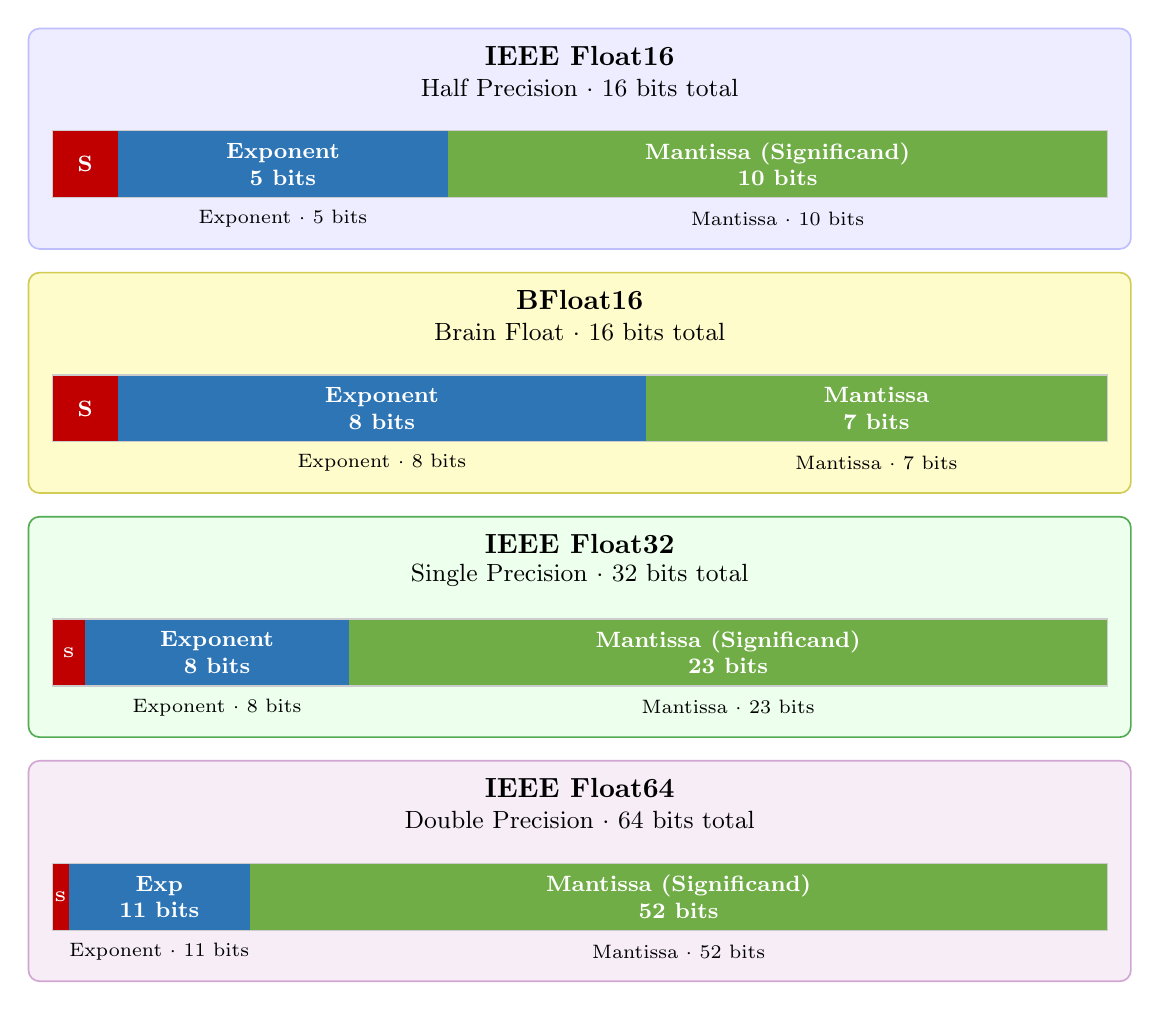
\begin{tikzpicture}[x=1cm, y=1cm]

  % ---- Color palette ----
  \definecolor{signcolor}{RGB}{192,0,0}     % red   -- sign bit
  \definecolor{expcolor} {RGB}{46,117,182}  % blue  -- exponent
  \definecolor{mancolor} {RGB}{112,173,71}  % green -- mantissa

  % ---- Panel backgrounds ----
  % Panels are 14 cm wide x 2.8 cm tall, separated by 0.3 cm gaps.
  % Y positions (bottom edge): Float16=9.30, BFloat16=6.20, Float32=3.10, Float64=0.00
  \draw[rounded corners=4pt, fill=blue!7,    draw=blue!25,        line width=0.6pt]
      (0.0,  9.30) rectangle (14.0, 12.10);  % Float16
  \draw[rounded corners=4pt, fill=yellow!20, draw=yellow!60!gray, line width=0.6pt]
      (0.0,  6.20) rectangle (14.0,  9.00);  % BFloat16
  \draw[rounded corners=4pt, fill=green!7,   draw=green!35!gray,  line width=0.6pt]
      (0.0,  3.10) rectangle (14.0,  5.90);  % Float32
  \draw[rounded corners=4pt, fill=violet!7,  draw=violet!35,      line width=0.6pt]
      (0.0,  0.00) rectangle (14.0,  2.80);  % Float64

  % ====================================================================
  % Bar geometry (shared across all panels):
  %   x range:    [0.30, 13.70]  => total bar width = 13.40 cm
  %   bar height: 0.85 cm
  %   bar bottom: panel_bottom + 0.65
  %   bar top:    panel_bottom + 1.50
  %
  % Segment x boundaries  (width = n_bits/total * 13.40):
  %   Float16  (16-bit): 0.300 | 1.138 | 5.325 | 13.700
  %   BFloat16 (16-bit): 0.300 | 1.138 | 7.838 | 13.700
  %   Float32  (32-bit): 0.300 | 0.719 | 4.069 | 13.700
  %   Float64  (64-bit): 0.300 | 0.509 | 2.813 | 13.700
  % ====================================================================

  % ------------------------------------------------------------------
  % IEEE Float16  (panel bottom y = 9.30)
  % ------------------------------------------------------------------
  \node[font=\normalsize\bfseries] at (7.0, 11.75) {IEEE Float16};
  \node[font=\small]               at (7.0, 11.35) {Half Precision $\cdot$ 16 bits total};

  % S:   1/16 * 13.40 = 0.838 cm   x: 0.300 -- 1.138,  center: 0.719
  \fill[signcolor] (0.300,  9.95) rectangle ( 1.138, 10.80);
  \node[text=white, font=\footnotesize\bfseries] at (0.719, 10.375) {S};

  % Exp: 5/16 * 13.40 = 4.188 cm   x: 1.138 -- 5.325,  center: 3.231
  \fill[expcolor]  (1.138,  9.95) rectangle ( 5.325, 10.80);
  \node[text=white, font=\footnotesize\bfseries, align=center] at (3.231, 10.375)
      {Exponent \\ 5 bits};

  % Man: 10/16 * 13.40 = 8.375 cm  x: 5.325 -- 13.700, center: 9.513
  \fill[mancolor]  (5.325,  9.95) rectangle (13.700, 10.80);
  \node[text=white, font=\footnotesize\bfseries, align=center] at (9.513, 10.375)
      {Mantissa (Significand) \\ 10 bits};

  \draw[black!20, line width=0.4pt] (0.300, 9.95) rectangle (13.700, 10.80);

  \node[font=\scriptsize] at (3.231, 9.68) {Exponent $\cdot$ 5 bits};
  \node[font=\scriptsize] at (9.513, 9.68) {Mantissa $\cdot$ 10 bits};

  % ------------------------------------------------------------------
  % BFloat16  (panel bottom y = 6.20)
  % ------------------------------------------------------------------
  \node[font=\normalsize\bfseries] at (7.0, 8.65) {BFloat16};
  \node[font=\small]               at (7.0, 8.25) {Brain Float $\cdot$ 16 bits total};

  % S:   1/16 * 13.40 = 0.838 cm   x: 0.300 -- 1.138,  center: 0.719
  \fill[signcolor] (0.300,  6.85) rectangle ( 1.138,  7.70);
  \node[text=white, font=\footnotesize\bfseries] at (0.719, 7.275) {S};

  % Exp: 8/16 * 13.40 = 6.700 cm   x: 1.138 -- 7.838,  center: 4.488
  \fill[expcolor]  (1.138,  6.85) rectangle ( 7.838,  7.70);
  \node[text=white, font=\footnotesize\bfseries, align=center] at (4.488, 7.275)
      {Exponent \\ 8 bits};

  % Man: 7/16 * 13.40 = 5.863 cm   x: 7.838 -- 13.700, center: 10.769
  \fill[mancolor]  (7.838,  6.85) rectangle (13.700,  7.70);
  \node[text=white, font=\footnotesize\bfseries, align=center] at (10.769, 7.275)
      {Mantissa \\ 7 bits};

  \draw[black!20, line width=0.4pt] (0.300, 6.85) rectangle (13.700, 7.70);

  \node[font=\scriptsize] at ( 4.488, 6.58) {Exponent $\cdot$ 8 bits};
  \node[font=\scriptsize] at (10.769, 6.58) {Mantissa $\cdot$ 7 bits};

  % ------------------------------------------------------------------
  % IEEE Float32  (panel bottom y = 3.10)
  % ------------------------------------------------------------------
  \node[font=\normalsize\bfseries] at (7.0, 5.55) {IEEE Float32};
  \node[font=\small]               at (7.0, 5.15) {Single Precision $\cdot$ 32 bits total};

  % S:   1/32 * 13.40 = 0.419 cm   x: 0.300 -- 0.719,  center: 0.510
  \fill[signcolor] (0.300,  3.75) rectangle ( 0.719,  4.60);
  \node[text=white, font=\tiny\bfseries] at (0.510, 4.175) {S};

  % Exp: 8/32 * 13.40 = 3.350 cm   x: 0.719 -- 4.069,  center: 2.394
  \fill[expcolor]  (0.719,  3.75) rectangle ( 4.069,  4.60);
  \node[text=white, font=\footnotesize\bfseries, align=center] at (2.394, 4.175)
      {Exponent \\ 8 bits};

  % Man: 23/32 * 13.40 = 9.631 cm  x: 4.069 -- 13.700, center: 8.885
  \fill[mancolor]  (4.069,  3.75) rectangle (13.700,  4.60);
  \node[text=white, font=\footnotesize\bfseries, align=center] at (8.885, 4.175)
      {Mantissa (Significand) \\ 23 bits};

  \draw[black!20, line width=0.4pt] (0.300, 3.75) rectangle (13.700, 4.60);

  \node[font=\scriptsize] at (2.394, 3.48) {Exponent $\cdot$ 8 bits};
  \node[font=\scriptsize] at (8.885, 3.48) {Mantissa $\cdot$ 23 bits};

  % ------------------------------------------------------------------
  % IEEE Float64  (panel bottom y = 0.00)
  % ------------------------------------------------------------------
  \node[font=\normalsize\bfseries] at (7.0, 2.45) {IEEE Float64};
  \node[font=\small]               at (7.0, 2.05) {Double Precision $\cdot$ 64 bits total};

  % S:    1/64 * 13.40 = 0.209 cm  x: 0.300 -- 0.509,  center: 0.405
  \fill[signcolor] (0.300,  0.65) rectangle ( 0.509,  1.50);
  \node[text=white, font=\tiny\bfseries] at (0.405, 1.075) {S};

  % Exp: 11/64 * 13.40 = 2.303 cm  x: 0.509 -- 2.813,  center: 1.661
  \fill[expcolor]  (0.509,  0.65) rectangle ( 2.813,  1.50);
  \node[text=white, font=\footnotesize\bfseries, align=center] at (1.661, 1.075)
      {Exp \\ 11 bits};

  % Man: 52/64 * 13.40 = 10.888 cm x: 2.813 -- 13.700, center: 8.257
  \fill[mancolor]  (2.813,  0.65) rectangle (13.700,  1.50);
  \node[text=white, font=\footnotesize\bfseries, align=center] at (8.257, 1.075)
      {Mantissa (Significand) \\ 52 bits};

  \draw[black!20, line width=0.4pt] (0.300, 0.65) rectangle (13.700, 1.50);

  \node[font=\scriptsize] at (1.661, 0.38) {Exponent $\cdot$ 11 bits};
  \node[font=\scriptsize] at (8.257, 0.38) {Mantissa $\cdot$ 52 bits};

\end{tikzpicture}
}
%
%   Fit to the full page width (~17.8 cm in IEEE two-column):
%     \resizebox{\textwidth}{!}{% Floating-point format comparison — single-column stack layout
%
% Required in preamble:
%   \usepackage{tikz}
%
% ---- Scaling -------------------------------------------------------
% The tikzpicture is drawn at its natural size: 14 cm wide x 12.1 cm tall.
% Use \resizebox (from the graphicx package, always loaded in IEEE style)
% to scale it to whatever width you need. The height adjusts automatically.
%
%   Fit to a single text column (~8.8 cm in IEEE two-column):
%     \resizebox{\columnwidth}{!}{\input{float_formats_tikz.tex}}
%
%   Fit to the full page width (~17.8 cm in IEEE two-column):
%     \resizebox{\textwidth}{!}{\input{float_formats_tikz.tex}}
%
%   Fit to an arbitrary fraction of the column width:
%     \resizebox{0.9\columnwidth}{!}{\input{float_formats_tikz.tex}}
%
% \resizebox scales everything uniformly — coordinates, line widths,
% and fonts — so the result looks identical regardless of the chosen width.
%
% Recommended figure wrapper (single column):
%   \begin{figure}[t]
%     \centering
%     \resizebox{\columnwidth}{!}{\input{float_formats_tikz.tex}}
%     \caption{...}
%     \label{fig:float-formats}
%   \end{figure}
% --------------------------------------------------------------------
%
% Layout: 4 panels stacked vertically, each 14 cm x 2.8 cm.
% Bar widths are proportional to actual bit-field widths.
%   Float16:  S=1, Exp=5,  Man=10  (16 bits total)
%   BFloat16: S=1, Exp=8,  Man=7   (16 bits total)
%   Float32:  S=1, Exp=8,  Man=23  (32 bits total)
%   Float64:  S=1, Exp=11, Man=52  (64 bits total)

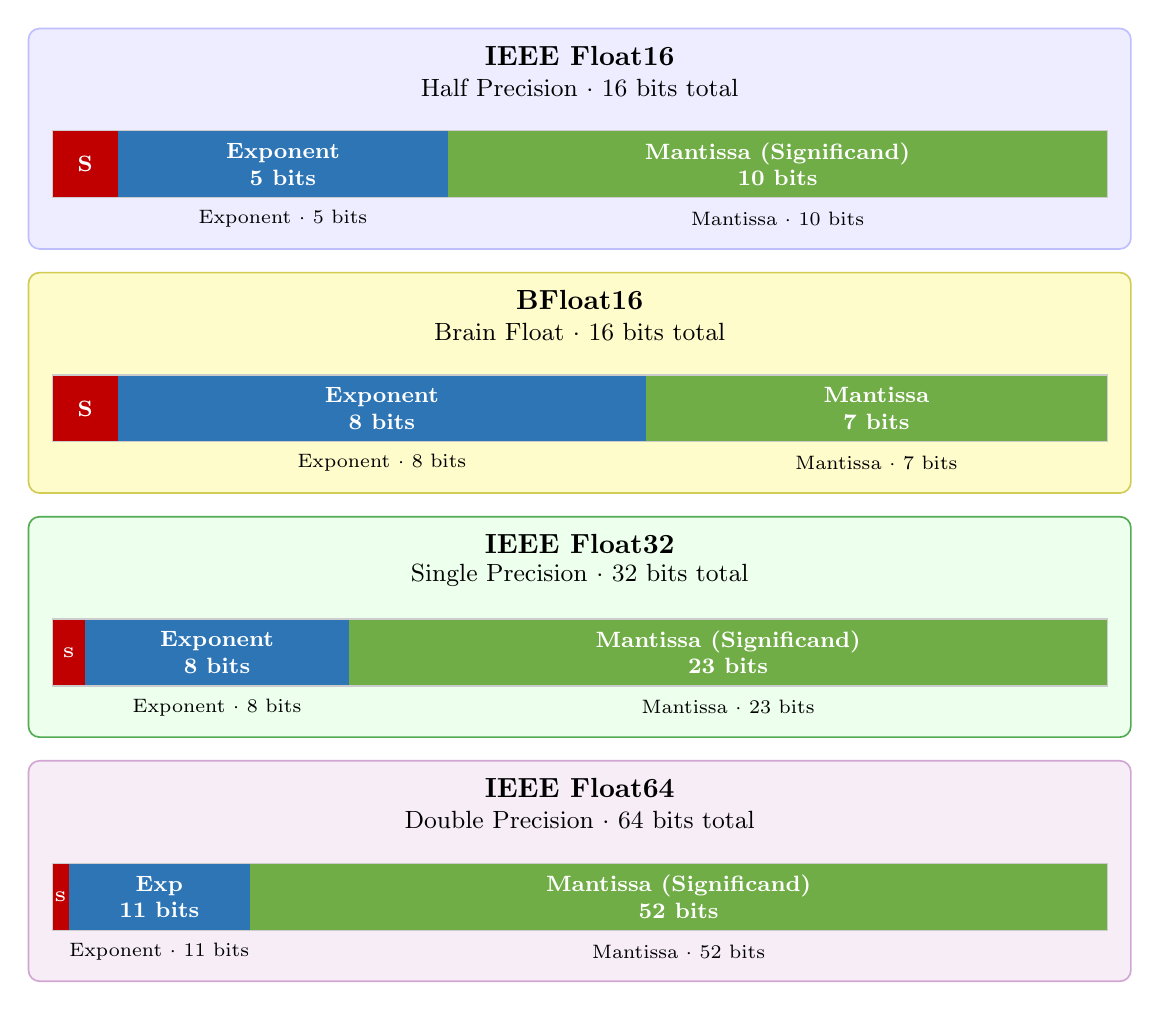
\begin{tikzpicture}[x=1cm, y=1cm]

  % ---- Color palette ----
  \definecolor{signcolor}{RGB}{192,0,0}     % red   -- sign bit
  \definecolor{expcolor} {RGB}{46,117,182}  % blue  -- exponent
  \definecolor{mancolor} {RGB}{112,173,71}  % green -- mantissa

  % ---- Panel backgrounds ----
  % Panels are 14 cm wide x 2.8 cm tall, separated by 0.3 cm gaps.
  % Y positions (bottom edge): Float16=9.30, BFloat16=6.20, Float32=3.10, Float64=0.00
  \draw[rounded corners=4pt, fill=blue!7,    draw=blue!25,        line width=0.6pt]
      (0.0,  9.30) rectangle (14.0, 12.10);  % Float16
  \draw[rounded corners=4pt, fill=yellow!20, draw=yellow!60!gray, line width=0.6pt]
      (0.0,  6.20) rectangle (14.0,  9.00);  % BFloat16
  \draw[rounded corners=4pt, fill=green!7,   draw=green!35!gray,  line width=0.6pt]
      (0.0,  3.10) rectangle (14.0,  5.90);  % Float32
  \draw[rounded corners=4pt, fill=violet!7,  draw=violet!35,      line width=0.6pt]
      (0.0,  0.00) rectangle (14.0,  2.80);  % Float64

  % ====================================================================
  % Bar geometry (shared across all panels):
  %   x range:    [0.30, 13.70]  => total bar width = 13.40 cm
  %   bar height: 0.85 cm
  %   bar bottom: panel_bottom + 0.65
  %   bar top:    panel_bottom + 1.50
  %
  % Segment x boundaries  (width = n_bits/total * 13.40):
  %   Float16  (16-bit): 0.300 | 1.138 | 5.325 | 13.700
  %   BFloat16 (16-bit): 0.300 | 1.138 | 7.838 | 13.700
  %   Float32  (32-bit): 0.300 | 0.719 | 4.069 | 13.700
  %   Float64  (64-bit): 0.300 | 0.509 | 2.813 | 13.700
  % ====================================================================

  % ------------------------------------------------------------------
  % IEEE Float16  (panel bottom y = 9.30)
  % ------------------------------------------------------------------
  \node[font=\normalsize\bfseries] at (7.0, 11.75) {IEEE Float16};
  \node[font=\small]               at (7.0, 11.35) {Half Precision $\cdot$ 16 bits total};

  % S:   1/16 * 13.40 = 0.838 cm   x: 0.300 -- 1.138,  center: 0.719
  \fill[signcolor] (0.300,  9.95) rectangle ( 1.138, 10.80);
  \node[text=white, font=\footnotesize\bfseries] at (0.719, 10.375) {S};

  % Exp: 5/16 * 13.40 = 4.188 cm   x: 1.138 -- 5.325,  center: 3.231
  \fill[expcolor]  (1.138,  9.95) rectangle ( 5.325, 10.80);
  \node[text=white, font=\footnotesize\bfseries, align=center] at (3.231, 10.375)
      {Exponent \\ 5 bits};

  % Man: 10/16 * 13.40 = 8.375 cm  x: 5.325 -- 13.700, center: 9.513
  \fill[mancolor]  (5.325,  9.95) rectangle (13.700, 10.80);
  \node[text=white, font=\footnotesize\bfseries, align=center] at (9.513, 10.375)
      {Mantissa (Significand) \\ 10 bits};

  \draw[black!20, line width=0.4pt] (0.300, 9.95) rectangle (13.700, 10.80);

  \node[font=\scriptsize] at (3.231, 9.68) {Exponent $\cdot$ 5 bits};
  \node[font=\scriptsize] at (9.513, 9.68) {Mantissa $\cdot$ 10 bits};

  % ------------------------------------------------------------------
  % BFloat16  (panel bottom y = 6.20)
  % ------------------------------------------------------------------
  \node[font=\normalsize\bfseries] at (7.0, 8.65) {BFloat16};
  \node[font=\small]               at (7.0, 8.25) {Brain Float $\cdot$ 16 bits total};

  % S:   1/16 * 13.40 = 0.838 cm   x: 0.300 -- 1.138,  center: 0.719
  \fill[signcolor] (0.300,  6.85) rectangle ( 1.138,  7.70);
  \node[text=white, font=\footnotesize\bfseries] at (0.719, 7.275) {S};

  % Exp: 8/16 * 13.40 = 6.700 cm   x: 1.138 -- 7.838,  center: 4.488
  \fill[expcolor]  (1.138,  6.85) rectangle ( 7.838,  7.70);
  \node[text=white, font=\footnotesize\bfseries, align=center] at (4.488, 7.275)
      {Exponent \\ 8 bits};

  % Man: 7/16 * 13.40 = 5.863 cm   x: 7.838 -- 13.700, center: 10.769
  \fill[mancolor]  (7.838,  6.85) rectangle (13.700,  7.70);
  \node[text=white, font=\footnotesize\bfseries, align=center] at (10.769, 7.275)
      {Mantissa \\ 7 bits};

  \draw[black!20, line width=0.4pt] (0.300, 6.85) rectangle (13.700, 7.70);

  \node[font=\scriptsize] at ( 4.488, 6.58) {Exponent $\cdot$ 8 bits};
  \node[font=\scriptsize] at (10.769, 6.58) {Mantissa $\cdot$ 7 bits};

  % ------------------------------------------------------------------
  % IEEE Float32  (panel bottom y = 3.10)
  % ------------------------------------------------------------------
  \node[font=\normalsize\bfseries] at (7.0, 5.55) {IEEE Float32};
  \node[font=\small]               at (7.0, 5.15) {Single Precision $\cdot$ 32 bits total};

  % S:   1/32 * 13.40 = 0.419 cm   x: 0.300 -- 0.719,  center: 0.510
  \fill[signcolor] (0.300,  3.75) rectangle ( 0.719,  4.60);
  \node[text=white, font=\tiny\bfseries] at (0.510, 4.175) {S};

  % Exp: 8/32 * 13.40 = 3.350 cm   x: 0.719 -- 4.069,  center: 2.394
  \fill[expcolor]  (0.719,  3.75) rectangle ( 4.069,  4.60);
  \node[text=white, font=\footnotesize\bfseries, align=center] at (2.394, 4.175)
      {Exponent \\ 8 bits};

  % Man: 23/32 * 13.40 = 9.631 cm  x: 4.069 -- 13.700, center: 8.885
  \fill[mancolor]  (4.069,  3.75) rectangle (13.700,  4.60);
  \node[text=white, font=\footnotesize\bfseries, align=center] at (8.885, 4.175)
      {Mantissa (Significand) \\ 23 bits};

  \draw[black!20, line width=0.4pt] (0.300, 3.75) rectangle (13.700, 4.60);

  \node[font=\scriptsize] at (2.394, 3.48) {Exponent $\cdot$ 8 bits};
  \node[font=\scriptsize] at (8.885, 3.48) {Mantissa $\cdot$ 23 bits};

  % ------------------------------------------------------------------
  % IEEE Float64  (panel bottom y = 0.00)
  % ------------------------------------------------------------------
  \node[font=\normalsize\bfseries] at (7.0, 2.45) {IEEE Float64};
  \node[font=\small]               at (7.0, 2.05) {Double Precision $\cdot$ 64 bits total};

  % S:    1/64 * 13.40 = 0.209 cm  x: 0.300 -- 0.509,  center: 0.405
  \fill[signcolor] (0.300,  0.65) rectangle ( 0.509,  1.50);
  \node[text=white, font=\tiny\bfseries] at (0.405, 1.075) {S};

  % Exp: 11/64 * 13.40 = 2.303 cm  x: 0.509 -- 2.813,  center: 1.661
  \fill[expcolor]  (0.509,  0.65) rectangle ( 2.813,  1.50);
  \node[text=white, font=\footnotesize\bfseries, align=center] at (1.661, 1.075)
      {Exp \\ 11 bits};

  % Man: 52/64 * 13.40 = 10.888 cm x: 2.813 -- 13.700, center: 8.257
  \fill[mancolor]  (2.813,  0.65) rectangle (13.700,  1.50);
  \node[text=white, font=\footnotesize\bfseries, align=center] at (8.257, 1.075)
      {Mantissa (Significand) \\ 52 bits};

  \draw[black!20, line width=0.4pt] (0.300, 0.65) rectangle (13.700, 1.50);

  \node[font=\scriptsize] at (1.661, 0.38) {Exponent $\cdot$ 11 bits};
  \node[font=\scriptsize] at (8.257, 0.38) {Mantissa $\cdot$ 52 bits};

\end{tikzpicture}
}
%
%   Fit to an arbitrary fraction of the column width:
%     \resizebox{0.9\columnwidth}{!}{% Floating-point format comparison — single-column stack layout
%
% Required in preamble:
%   \usepackage{tikz}
%
% ---- Scaling -------------------------------------------------------
% The tikzpicture is drawn at its natural size: 14 cm wide x 12.1 cm tall.
% Use \resizebox (from the graphicx package, always loaded in IEEE style)
% to scale it to whatever width you need. The height adjusts automatically.
%
%   Fit to a single text column (~8.8 cm in IEEE two-column):
%     \resizebox{\columnwidth}{!}{\input{float_formats_tikz.tex}}
%
%   Fit to the full page width (~17.8 cm in IEEE two-column):
%     \resizebox{\textwidth}{!}{\input{float_formats_tikz.tex}}
%
%   Fit to an arbitrary fraction of the column width:
%     \resizebox{0.9\columnwidth}{!}{\input{float_formats_tikz.tex}}
%
% \resizebox scales everything uniformly — coordinates, line widths,
% and fonts — so the result looks identical regardless of the chosen width.
%
% Recommended figure wrapper (single column):
%   \begin{figure}[t]
%     \centering
%     \resizebox{\columnwidth}{!}{\input{float_formats_tikz.tex}}
%     \caption{...}
%     \label{fig:float-formats}
%   \end{figure}
% --------------------------------------------------------------------
%
% Layout: 4 panels stacked vertically, each 14 cm x 2.8 cm.
% Bar widths are proportional to actual bit-field widths.
%   Float16:  S=1, Exp=5,  Man=10  (16 bits total)
%   BFloat16: S=1, Exp=8,  Man=7   (16 bits total)
%   Float32:  S=1, Exp=8,  Man=23  (32 bits total)
%   Float64:  S=1, Exp=11, Man=52  (64 bits total)

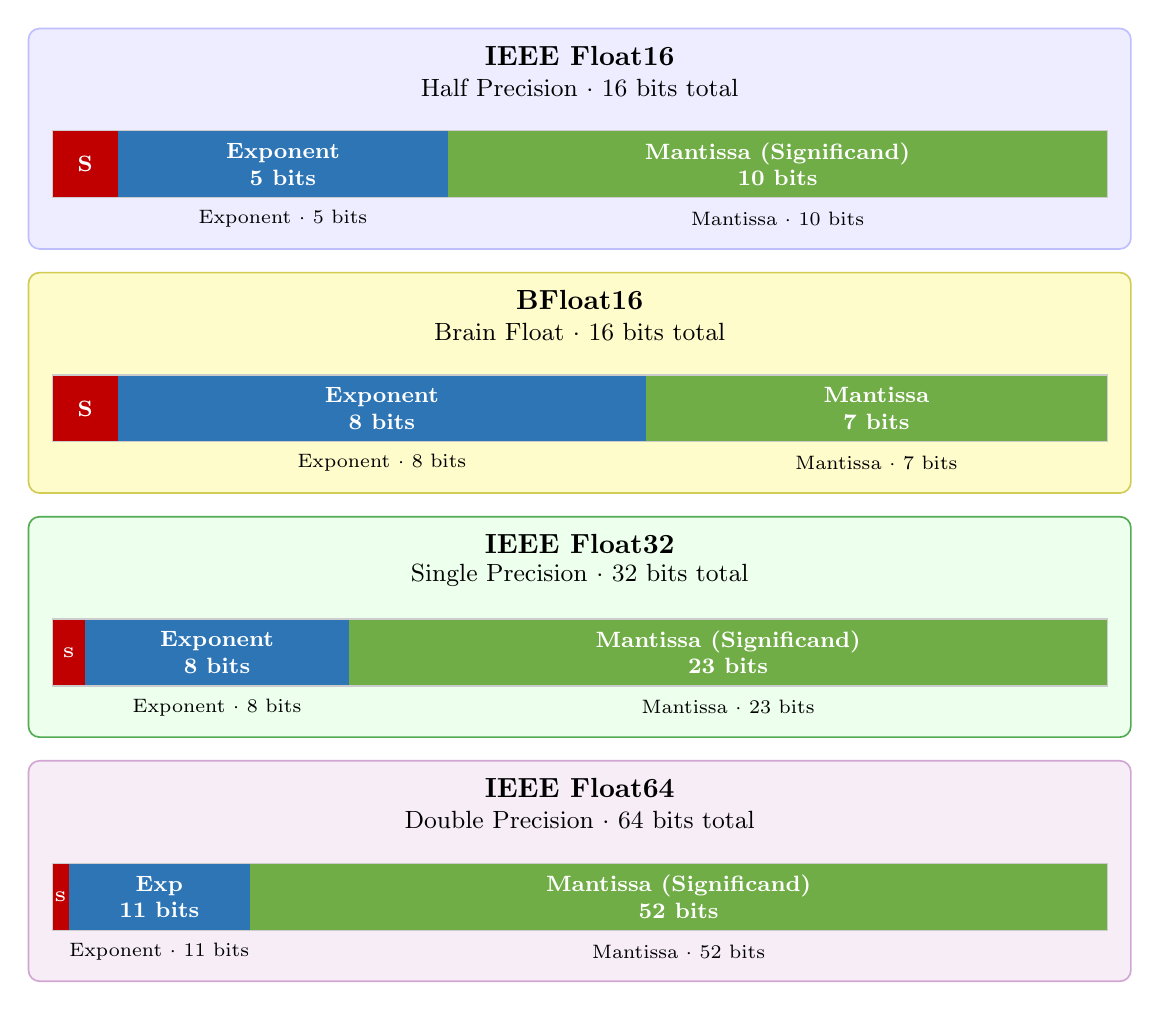
\begin{tikzpicture}[x=1cm, y=1cm]

  % ---- Color palette ----
  \definecolor{signcolor}{RGB}{192,0,0}     % red   -- sign bit
  \definecolor{expcolor} {RGB}{46,117,182}  % blue  -- exponent
  \definecolor{mancolor} {RGB}{112,173,71}  % green -- mantissa

  % ---- Panel backgrounds ----
  % Panels are 14 cm wide x 2.8 cm tall, separated by 0.3 cm gaps.
  % Y positions (bottom edge): Float16=9.30, BFloat16=6.20, Float32=3.10, Float64=0.00
  \draw[rounded corners=4pt, fill=blue!7,    draw=blue!25,        line width=0.6pt]
      (0.0,  9.30) rectangle (14.0, 12.10);  % Float16
  \draw[rounded corners=4pt, fill=yellow!20, draw=yellow!60!gray, line width=0.6pt]
      (0.0,  6.20) rectangle (14.0,  9.00);  % BFloat16
  \draw[rounded corners=4pt, fill=green!7,   draw=green!35!gray,  line width=0.6pt]
      (0.0,  3.10) rectangle (14.0,  5.90);  % Float32
  \draw[rounded corners=4pt, fill=violet!7,  draw=violet!35,      line width=0.6pt]
      (0.0,  0.00) rectangle (14.0,  2.80);  % Float64

  % ====================================================================
  % Bar geometry (shared across all panels):
  %   x range:    [0.30, 13.70]  => total bar width = 13.40 cm
  %   bar height: 0.85 cm
  %   bar bottom: panel_bottom + 0.65
  %   bar top:    panel_bottom + 1.50
  %
  % Segment x boundaries  (width = n_bits/total * 13.40):
  %   Float16  (16-bit): 0.300 | 1.138 | 5.325 | 13.700
  %   BFloat16 (16-bit): 0.300 | 1.138 | 7.838 | 13.700
  %   Float32  (32-bit): 0.300 | 0.719 | 4.069 | 13.700
  %   Float64  (64-bit): 0.300 | 0.509 | 2.813 | 13.700
  % ====================================================================

  % ------------------------------------------------------------------
  % IEEE Float16  (panel bottom y = 9.30)
  % ------------------------------------------------------------------
  \node[font=\normalsize\bfseries] at (7.0, 11.75) {IEEE Float16};
  \node[font=\small]               at (7.0, 11.35) {Half Precision $\cdot$ 16 bits total};

  % S:   1/16 * 13.40 = 0.838 cm   x: 0.300 -- 1.138,  center: 0.719
  \fill[signcolor] (0.300,  9.95) rectangle ( 1.138, 10.80);
  \node[text=white, font=\footnotesize\bfseries] at (0.719, 10.375) {S};

  % Exp: 5/16 * 13.40 = 4.188 cm   x: 1.138 -- 5.325,  center: 3.231
  \fill[expcolor]  (1.138,  9.95) rectangle ( 5.325, 10.80);
  \node[text=white, font=\footnotesize\bfseries, align=center] at (3.231, 10.375)
      {Exponent \\ 5 bits};

  % Man: 10/16 * 13.40 = 8.375 cm  x: 5.325 -- 13.700, center: 9.513
  \fill[mancolor]  (5.325,  9.95) rectangle (13.700, 10.80);
  \node[text=white, font=\footnotesize\bfseries, align=center] at (9.513, 10.375)
      {Mantissa (Significand) \\ 10 bits};

  \draw[black!20, line width=0.4pt] (0.300, 9.95) rectangle (13.700, 10.80);

  \node[font=\scriptsize] at (3.231, 9.68) {Exponent $\cdot$ 5 bits};
  \node[font=\scriptsize] at (9.513, 9.68) {Mantissa $\cdot$ 10 bits};

  % ------------------------------------------------------------------
  % BFloat16  (panel bottom y = 6.20)
  % ------------------------------------------------------------------
  \node[font=\normalsize\bfseries] at (7.0, 8.65) {BFloat16};
  \node[font=\small]               at (7.0, 8.25) {Brain Float $\cdot$ 16 bits total};

  % S:   1/16 * 13.40 = 0.838 cm   x: 0.300 -- 1.138,  center: 0.719
  \fill[signcolor] (0.300,  6.85) rectangle ( 1.138,  7.70);
  \node[text=white, font=\footnotesize\bfseries] at (0.719, 7.275) {S};

  % Exp: 8/16 * 13.40 = 6.700 cm   x: 1.138 -- 7.838,  center: 4.488
  \fill[expcolor]  (1.138,  6.85) rectangle ( 7.838,  7.70);
  \node[text=white, font=\footnotesize\bfseries, align=center] at (4.488, 7.275)
      {Exponent \\ 8 bits};

  % Man: 7/16 * 13.40 = 5.863 cm   x: 7.838 -- 13.700, center: 10.769
  \fill[mancolor]  (7.838,  6.85) rectangle (13.700,  7.70);
  \node[text=white, font=\footnotesize\bfseries, align=center] at (10.769, 7.275)
      {Mantissa \\ 7 bits};

  \draw[black!20, line width=0.4pt] (0.300, 6.85) rectangle (13.700, 7.70);

  \node[font=\scriptsize] at ( 4.488, 6.58) {Exponent $\cdot$ 8 bits};
  \node[font=\scriptsize] at (10.769, 6.58) {Mantissa $\cdot$ 7 bits};

  % ------------------------------------------------------------------
  % IEEE Float32  (panel bottom y = 3.10)
  % ------------------------------------------------------------------
  \node[font=\normalsize\bfseries] at (7.0, 5.55) {IEEE Float32};
  \node[font=\small]               at (7.0, 5.15) {Single Precision $\cdot$ 32 bits total};

  % S:   1/32 * 13.40 = 0.419 cm   x: 0.300 -- 0.719,  center: 0.510
  \fill[signcolor] (0.300,  3.75) rectangle ( 0.719,  4.60);
  \node[text=white, font=\tiny\bfseries] at (0.510, 4.175) {S};

  % Exp: 8/32 * 13.40 = 3.350 cm   x: 0.719 -- 4.069,  center: 2.394
  \fill[expcolor]  (0.719,  3.75) rectangle ( 4.069,  4.60);
  \node[text=white, font=\footnotesize\bfseries, align=center] at (2.394, 4.175)
      {Exponent \\ 8 bits};

  % Man: 23/32 * 13.40 = 9.631 cm  x: 4.069 -- 13.700, center: 8.885
  \fill[mancolor]  (4.069,  3.75) rectangle (13.700,  4.60);
  \node[text=white, font=\footnotesize\bfseries, align=center] at (8.885, 4.175)
      {Mantissa (Significand) \\ 23 bits};

  \draw[black!20, line width=0.4pt] (0.300, 3.75) rectangle (13.700, 4.60);

  \node[font=\scriptsize] at (2.394, 3.48) {Exponent $\cdot$ 8 bits};
  \node[font=\scriptsize] at (8.885, 3.48) {Mantissa $\cdot$ 23 bits};

  % ------------------------------------------------------------------
  % IEEE Float64  (panel bottom y = 0.00)
  % ------------------------------------------------------------------
  \node[font=\normalsize\bfseries] at (7.0, 2.45) {IEEE Float64};
  \node[font=\small]               at (7.0, 2.05) {Double Precision $\cdot$ 64 bits total};

  % S:    1/64 * 13.40 = 0.209 cm  x: 0.300 -- 0.509,  center: 0.405
  \fill[signcolor] (0.300,  0.65) rectangle ( 0.509,  1.50);
  \node[text=white, font=\tiny\bfseries] at (0.405, 1.075) {S};

  % Exp: 11/64 * 13.40 = 2.303 cm  x: 0.509 -- 2.813,  center: 1.661
  \fill[expcolor]  (0.509,  0.65) rectangle ( 2.813,  1.50);
  \node[text=white, font=\footnotesize\bfseries, align=center] at (1.661, 1.075)
      {Exp \\ 11 bits};

  % Man: 52/64 * 13.40 = 10.888 cm x: 2.813 -- 13.700, center: 8.257
  \fill[mancolor]  (2.813,  0.65) rectangle (13.700,  1.50);
  \node[text=white, font=\footnotesize\bfseries, align=center] at (8.257, 1.075)
      {Mantissa (Significand) \\ 52 bits};

  \draw[black!20, line width=0.4pt] (0.300, 0.65) rectangle (13.700, 1.50);

  \node[font=\scriptsize] at (1.661, 0.38) {Exponent $\cdot$ 11 bits};
  \node[font=\scriptsize] at (8.257, 0.38) {Mantissa $\cdot$ 52 bits};

\end{tikzpicture}
}
%
% \resizebox scales everything uniformly — coordinates, line widths,
% and fonts — so the result looks identical regardless of the chosen width.
%
% Recommended figure wrapper (single column):
%   \begin{figure}[t]
%     \centering
%     \resizebox{\columnwidth}{!}{% Floating-point format comparison — single-column stack layout
%
% Required in preamble:
%   \usepackage{tikz}
%
% ---- Scaling -------------------------------------------------------
% The tikzpicture is drawn at its natural size: 14 cm wide x 12.1 cm tall.
% Use \resizebox (from the graphicx package, always loaded in IEEE style)
% to scale it to whatever width you need. The height adjusts automatically.
%
%   Fit to a single text column (~8.8 cm in IEEE two-column):
%     \resizebox{\columnwidth}{!}{\input{float_formats_tikz.tex}}
%
%   Fit to the full page width (~17.8 cm in IEEE two-column):
%     \resizebox{\textwidth}{!}{\input{float_formats_tikz.tex}}
%
%   Fit to an arbitrary fraction of the column width:
%     \resizebox{0.9\columnwidth}{!}{\input{float_formats_tikz.tex}}
%
% \resizebox scales everything uniformly — coordinates, line widths,
% and fonts — so the result looks identical regardless of the chosen width.
%
% Recommended figure wrapper (single column):
%   \begin{figure}[t]
%     \centering
%     \resizebox{\columnwidth}{!}{\input{float_formats_tikz.tex}}
%     \caption{...}
%     \label{fig:float-formats}
%   \end{figure}
% --------------------------------------------------------------------
%
% Layout: 4 panels stacked vertically, each 14 cm x 2.8 cm.
% Bar widths are proportional to actual bit-field widths.
%   Float16:  S=1, Exp=5,  Man=10  (16 bits total)
%   BFloat16: S=1, Exp=8,  Man=7   (16 bits total)
%   Float32:  S=1, Exp=8,  Man=23  (32 bits total)
%   Float64:  S=1, Exp=11, Man=52  (64 bits total)

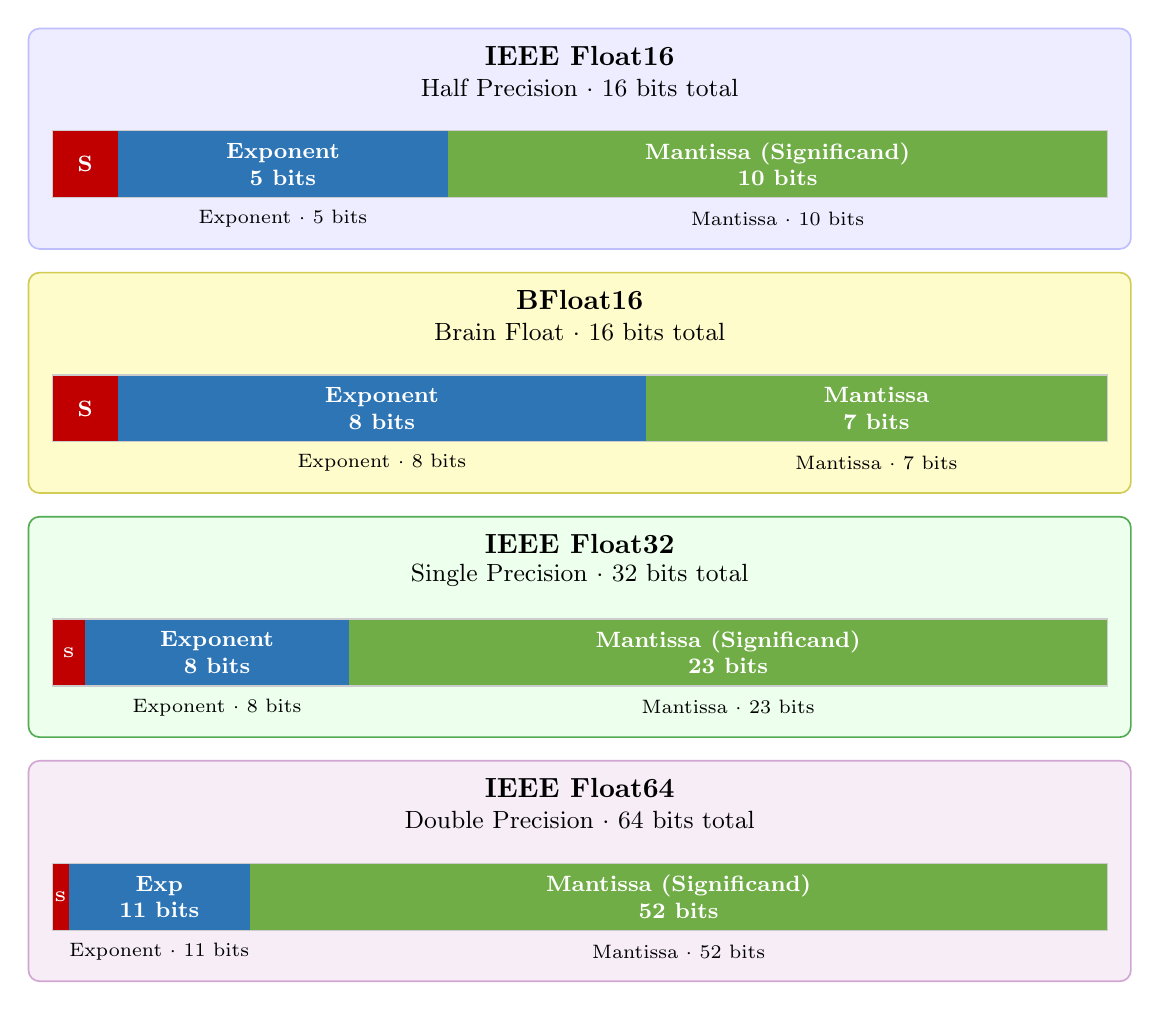
\begin{tikzpicture}[x=1cm, y=1cm]

  % ---- Color palette ----
  \definecolor{signcolor}{RGB}{192,0,0}     % red   -- sign bit
  \definecolor{expcolor} {RGB}{46,117,182}  % blue  -- exponent
  \definecolor{mancolor} {RGB}{112,173,71}  % green -- mantissa

  % ---- Panel backgrounds ----
  % Panels are 14 cm wide x 2.8 cm tall, separated by 0.3 cm gaps.
  % Y positions (bottom edge): Float16=9.30, BFloat16=6.20, Float32=3.10, Float64=0.00
  \draw[rounded corners=4pt, fill=blue!7,    draw=blue!25,        line width=0.6pt]
      (0.0,  9.30) rectangle (14.0, 12.10);  % Float16
  \draw[rounded corners=4pt, fill=yellow!20, draw=yellow!60!gray, line width=0.6pt]
      (0.0,  6.20) rectangle (14.0,  9.00);  % BFloat16
  \draw[rounded corners=4pt, fill=green!7,   draw=green!35!gray,  line width=0.6pt]
      (0.0,  3.10) rectangle (14.0,  5.90);  % Float32
  \draw[rounded corners=4pt, fill=violet!7,  draw=violet!35,      line width=0.6pt]
      (0.0,  0.00) rectangle (14.0,  2.80);  % Float64

  % ====================================================================
  % Bar geometry (shared across all panels):
  %   x range:    [0.30, 13.70]  => total bar width = 13.40 cm
  %   bar height: 0.85 cm
  %   bar bottom: panel_bottom + 0.65
  %   bar top:    panel_bottom + 1.50
  %
  % Segment x boundaries  (width = n_bits/total * 13.40):
  %   Float16  (16-bit): 0.300 | 1.138 | 5.325 | 13.700
  %   BFloat16 (16-bit): 0.300 | 1.138 | 7.838 | 13.700
  %   Float32  (32-bit): 0.300 | 0.719 | 4.069 | 13.700
  %   Float64  (64-bit): 0.300 | 0.509 | 2.813 | 13.700
  % ====================================================================

  % ------------------------------------------------------------------
  % IEEE Float16  (panel bottom y = 9.30)
  % ------------------------------------------------------------------
  \node[font=\normalsize\bfseries] at (7.0, 11.75) {IEEE Float16};
  \node[font=\small]               at (7.0, 11.35) {Half Precision $\cdot$ 16 bits total};

  % S:   1/16 * 13.40 = 0.838 cm   x: 0.300 -- 1.138,  center: 0.719
  \fill[signcolor] (0.300,  9.95) rectangle ( 1.138, 10.80);
  \node[text=white, font=\footnotesize\bfseries] at (0.719, 10.375) {S};

  % Exp: 5/16 * 13.40 = 4.188 cm   x: 1.138 -- 5.325,  center: 3.231
  \fill[expcolor]  (1.138,  9.95) rectangle ( 5.325, 10.80);
  \node[text=white, font=\footnotesize\bfseries, align=center] at (3.231, 10.375)
      {Exponent \\ 5 bits};

  % Man: 10/16 * 13.40 = 8.375 cm  x: 5.325 -- 13.700, center: 9.513
  \fill[mancolor]  (5.325,  9.95) rectangle (13.700, 10.80);
  \node[text=white, font=\footnotesize\bfseries, align=center] at (9.513, 10.375)
      {Mantissa (Significand) \\ 10 bits};

  \draw[black!20, line width=0.4pt] (0.300, 9.95) rectangle (13.700, 10.80);

  \node[font=\scriptsize] at (3.231, 9.68) {Exponent $\cdot$ 5 bits};
  \node[font=\scriptsize] at (9.513, 9.68) {Mantissa $\cdot$ 10 bits};

  % ------------------------------------------------------------------
  % BFloat16  (panel bottom y = 6.20)
  % ------------------------------------------------------------------
  \node[font=\normalsize\bfseries] at (7.0, 8.65) {BFloat16};
  \node[font=\small]               at (7.0, 8.25) {Brain Float $\cdot$ 16 bits total};

  % S:   1/16 * 13.40 = 0.838 cm   x: 0.300 -- 1.138,  center: 0.719
  \fill[signcolor] (0.300,  6.85) rectangle ( 1.138,  7.70);
  \node[text=white, font=\footnotesize\bfseries] at (0.719, 7.275) {S};

  % Exp: 8/16 * 13.40 = 6.700 cm   x: 1.138 -- 7.838,  center: 4.488
  \fill[expcolor]  (1.138,  6.85) rectangle ( 7.838,  7.70);
  \node[text=white, font=\footnotesize\bfseries, align=center] at (4.488, 7.275)
      {Exponent \\ 8 bits};

  % Man: 7/16 * 13.40 = 5.863 cm   x: 7.838 -- 13.700, center: 10.769
  \fill[mancolor]  (7.838,  6.85) rectangle (13.700,  7.70);
  \node[text=white, font=\footnotesize\bfseries, align=center] at (10.769, 7.275)
      {Mantissa \\ 7 bits};

  \draw[black!20, line width=0.4pt] (0.300, 6.85) rectangle (13.700, 7.70);

  \node[font=\scriptsize] at ( 4.488, 6.58) {Exponent $\cdot$ 8 bits};
  \node[font=\scriptsize] at (10.769, 6.58) {Mantissa $\cdot$ 7 bits};

  % ------------------------------------------------------------------
  % IEEE Float32  (panel bottom y = 3.10)
  % ------------------------------------------------------------------
  \node[font=\normalsize\bfseries] at (7.0, 5.55) {IEEE Float32};
  \node[font=\small]               at (7.0, 5.15) {Single Precision $\cdot$ 32 bits total};

  % S:   1/32 * 13.40 = 0.419 cm   x: 0.300 -- 0.719,  center: 0.510
  \fill[signcolor] (0.300,  3.75) rectangle ( 0.719,  4.60);
  \node[text=white, font=\tiny\bfseries] at (0.510, 4.175) {S};

  % Exp: 8/32 * 13.40 = 3.350 cm   x: 0.719 -- 4.069,  center: 2.394
  \fill[expcolor]  (0.719,  3.75) rectangle ( 4.069,  4.60);
  \node[text=white, font=\footnotesize\bfseries, align=center] at (2.394, 4.175)
      {Exponent \\ 8 bits};

  % Man: 23/32 * 13.40 = 9.631 cm  x: 4.069 -- 13.700, center: 8.885
  \fill[mancolor]  (4.069,  3.75) rectangle (13.700,  4.60);
  \node[text=white, font=\footnotesize\bfseries, align=center] at (8.885, 4.175)
      {Mantissa (Significand) \\ 23 bits};

  \draw[black!20, line width=0.4pt] (0.300, 3.75) rectangle (13.700, 4.60);

  \node[font=\scriptsize] at (2.394, 3.48) {Exponent $\cdot$ 8 bits};
  \node[font=\scriptsize] at (8.885, 3.48) {Mantissa $\cdot$ 23 bits};

  % ------------------------------------------------------------------
  % IEEE Float64  (panel bottom y = 0.00)
  % ------------------------------------------------------------------
  \node[font=\normalsize\bfseries] at (7.0, 2.45) {IEEE Float64};
  \node[font=\small]               at (7.0, 2.05) {Double Precision $\cdot$ 64 bits total};

  % S:    1/64 * 13.40 = 0.209 cm  x: 0.300 -- 0.509,  center: 0.405
  \fill[signcolor] (0.300,  0.65) rectangle ( 0.509,  1.50);
  \node[text=white, font=\tiny\bfseries] at (0.405, 1.075) {S};

  % Exp: 11/64 * 13.40 = 2.303 cm  x: 0.509 -- 2.813,  center: 1.661
  \fill[expcolor]  (0.509,  0.65) rectangle ( 2.813,  1.50);
  \node[text=white, font=\footnotesize\bfseries, align=center] at (1.661, 1.075)
      {Exp \\ 11 bits};

  % Man: 52/64 * 13.40 = 10.888 cm x: 2.813 -- 13.700, center: 8.257
  \fill[mancolor]  (2.813,  0.65) rectangle (13.700,  1.50);
  \node[text=white, font=\footnotesize\bfseries, align=center] at (8.257, 1.075)
      {Mantissa (Significand) \\ 52 bits};

  \draw[black!20, line width=0.4pt] (0.300, 0.65) rectangle (13.700, 1.50);

  \node[font=\scriptsize] at (1.661, 0.38) {Exponent $\cdot$ 11 bits};
  \node[font=\scriptsize] at (8.257, 0.38) {Mantissa $\cdot$ 52 bits};

\end{tikzpicture}
}
%     \caption{...}
%     \label{fig:float-formats}
%   \end{figure}
% --------------------------------------------------------------------
%
% Layout: 4 panels stacked vertically, each 14 cm x 2.8 cm.
% Bar widths are proportional to actual bit-field widths.
%   Float16:  S=1, Exp=5,  Man=10  (16 bits total)
%   BFloat16: S=1, Exp=8,  Man=7   (16 bits total)
%   Float32:  S=1, Exp=8,  Man=23  (32 bits total)
%   Float64:  S=1, Exp=11, Man=52  (64 bits total)

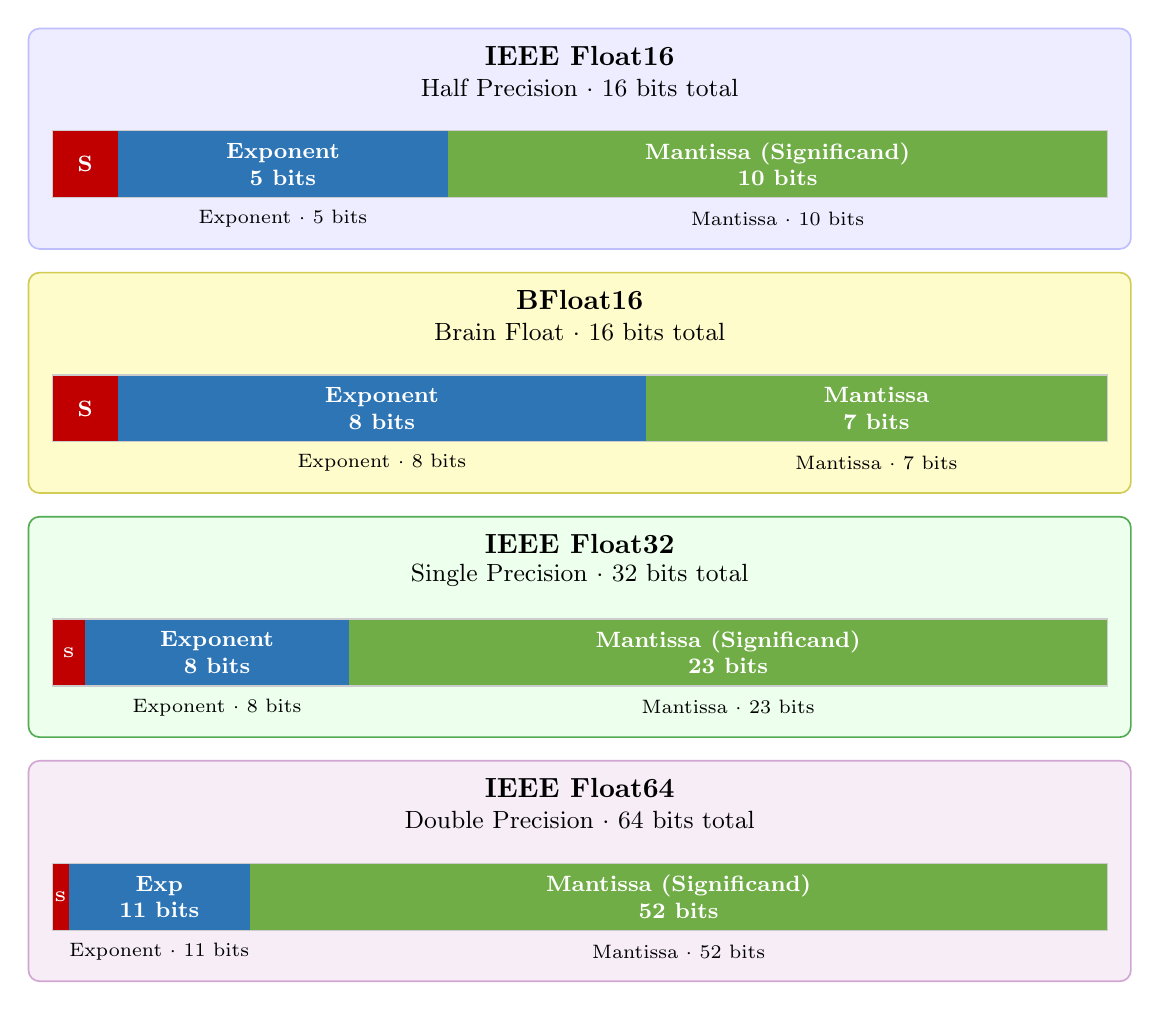
\begin{tikzpicture}[x=1cm, y=1cm]

  % ---- Color palette ----
  \definecolor{signcolor}{RGB}{192,0,0}     % red   -- sign bit
  \definecolor{expcolor} {RGB}{46,117,182}  % blue  -- exponent
  \definecolor{mancolor} {RGB}{112,173,71}  % green -- mantissa

  % ---- Panel backgrounds ----
  % Panels are 14 cm wide x 2.8 cm tall, separated by 0.3 cm gaps.
  % Y positions (bottom edge): Float16=9.30, BFloat16=6.20, Float32=3.10, Float64=0.00
  \draw[rounded corners=4pt, fill=blue!7,    draw=blue!25,        line width=0.6pt]
      (0.0,  9.30) rectangle (14.0, 12.10);  % Float16
  \draw[rounded corners=4pt, fill=yellow!20, draw=yellow!60!gray, line width=0.6pt]
      (0.0,  6.20) rectangle (14.0,  9.00);  % BFloat16
  \draw[rounded corners=4pt, fill=green!7,   draw=green!35!gray,  line width=0.6pt]
      (0.0,  3.10) rectangle (14.0,  5.90);  % Float32
  \draw[rounded corners=4pt, fill=violet!7,  draw=violet!35,      line width=0.6pt]
      (0.0,  0.00) rectangle (14.0,  2.80);  % Float64

  % ====================================================================
  % Bar geometry (shared across all panels):
  %   x range:    [0.30, 13.70]  => total bar width = 13.40 cm
  %   bar height: 0.85 cm
  %   bar bottom: panel_bottom + 0.65
  %   bar top:    panel_bottom + 1.50
  %
  % Segment x boundaries  (width = n_bits/total * 13.40):
  %   Float16  (16-bit): 0.300 | 1.138 | 5.325 | 13.700
  %   BFloat16 (16-bit): 0.300 | 1.138 | 7.838 | 13.700
  %   Float32  (32-bit): 0.300 | 0.719 | 4.069 | 13.700
  %   Float64  (64-bit): 0.300 | 0.509 | 2.813 | 13.700
  % ====================================================================

  % ------------------------------------------------------------------
  % IEEE Float16  (panel bottom y = 9.30)
  % ------------------------------------------------------------------
  \node[font=\normalsize\bfseries] at (7.0, 11.75) {IEEE Float16};
  \node[font=\small]               at (7.0, 11.35) {Half Precision $\cdot$ 16 bits total};

  % S:   1/16 * 13.40 = 0.838 cm   x: 0.300 -- 1.138,  center: 0.719
  \fill[signcolor] (0.300,  9.95) rectangle ( 1.138, 10.80);
  \node[text=white, font=\footnotesize\bfseries] at (0.719, 10.375) {S};

  % Exp: 5/16 * 13.40 = 4.188 cm   x: 1.138 -- 5.325,  center: 3.231
  \fill[expcolor]  (1.138,  9.95) rectangle ( 5.325, 10.80);
  \node[text=white, font=\footnotesize\bfseries, align=center] at (3.231, 10.375)
      {Exponent \\ 5 bits};

  % Man: 10/16 * 13.40 = 8.375 cm  x: 5.325 -- 13.700, center: 9.513
  \fill[mancolor]  (5.325,  9.95) rectangle (13.700, 10.80);
  \node[text=white, font=\footnotesize\bfseries, align=center] at (9.513, 10.375)
      {Mantissa (Significand) \\ 10 bits};

  \draw[black!20, line width=0.4pt] (0.300, 9.95) rectangle (13.700, 10.80);

  \node[font=\scriptsize] at (3.231, 9.68) {Exponent $\cdot$ 5 bits};
  \node[font=\scriptsize] at (9.513, 9.68) {Mantissa $\cdot$ 10 bits};

  % ------------------------------------------------------------------
  % BFloat16  (panel bottom y = 6.20)
  % ------------------------------------------------------------------
  \node[font=\normalsize\bfseries] at (7.0, 8.65) {BFloat16};
  \node[font=\small]               at (7.0, 8.25) {Brain Float $\cdot$ 16 bits total};

  % S:   1/16 * 13.40 = 0.838 cm   x: 0.300 -- 1.138,  center: 0.719
  \fill[signcolor] (0.300,  6.85) rectangle ( 1.138,  7.70);
  \node[text=white, font=\footnotesize\bfseries] at (0.719, 7.275) {S};

  % Exp: 8/16 * 13.40 = 6.700 cm   x: 1.138 -- 7.838,  center: 4.488
  \fill[expcolor]  (1.138,  6.85) rectangle ( 7.838,  7.70);
  \node[text=white, font=\footnotesize\bfseries, align=center] at (4.488, 7.275)
      {Exponent \\ 8 bits};

  % Man: 7/16 * 13.40 = 5.863 cm   x: 7.838 -- 13.700, center: 10.769
  \fill[mancolor]  (7.838,  6.85) rectangle (13.700,  7.70);
  \node[text=white, font=\footnotesize\bfseries, align=center] at (10.769, 7.275)
      {Mantissa \\ 7 bits};

  \draw[black!20, line width=0.4pt] (0.300, 6.85) rectangle (13.700, 7.70);

  \node[font=\scriptsize] at ( 4.488, 6.58) {Exponent $\cdot$ 8 bits};
  \node[font=\scriptsize] at (10.769, 6.58) {Mantissa $\cdot$ 7 bits};

  % ------------------------------------------------------------------
  % IEEE Float32  (panel bottom y = 3.10)
  % ------------------------------------------------------------------
  \node[font=\normalsize\bfseries] at (7.0, 5.55) {IEEE Float32};
  \node[font=\small]               at (7.0, 5.15) {Single Precision $\cdot$ 32 bits total};

  % S:   1/32 * 13.40 = 0.419 cm   x: 0.300 -- 0.719,  center: 0.510
  \fill[signcolor] (0.300,  3.75) rectangle ( 0.719,  4.60);
  \node[text=white, font=\tiny\bfseries] at (0.510, 4.175) {S};

  % Exp: 8/32 * 13.40 = 3.350 cm   x: 0.719 -- 4.069,  center: 2.394
  \fill[expcolor]  (0.719,  3.75) rectangle ( 4.069,  4.60);
  \node[text=white, font=\footnotesize\bfseries, align=center] at (2.394, 4.175)
      {Exponent \\ 8 bits};

  % Man: 23/32 * 13.40 = 9.631 cm  x: 4.069 -- 13.700, center: 8.885
  \fill[mancolor]  (4.069,  3.75) rectangle (13.700,  4.60);
  \node[text=white, font=\footnotesize\bfseries, align=center] at (8.885, 4.175)
      {Mantissa (Significand) \\ 23 bits};

  \draw[black!20, line width=0.4pt] (0.300, 3.75) rectangle (13.700, 4.60);

  \node[font=\scriptsize] at (2.394, 3.48) {Exponent $\cdot$ 8 bits};
  \node[font=\scriptsize] at (8.885, 3.48) {Mantissa $\cdot$ 23 bits};

  % ------------------------------------------------------------------
  % IEEE Float64  (panel bottom y = 0.00)
  % ------------------------------------------------------------------
  \node[font=\normalsize\bfseries] at (7.0, 2.45) {IEEE Float64};
  \node[font=\small]               at (7.0, 2.05) {Double Precision $\cdot$ 64 bits total};

  % S:    1/64 * 13.40 = 0.209 cm  x: 0.300 -- 0.509,  center: 0.405
  \fill[signcolor] (0.300,  0.65) rectangle ( 0.509,  1.50);
  \node[text=white, font=\tiny\bfseries] at (0.405, 1.075) {S};

  % Exp: 11/64 * 13.40 = 2.303 cm  x: 0.509 -- 2.813,  center: 1.661
  \fill[expcolor]  (0.509,  0.65) rectangle ( 2.813,  1.50);
  \node[text=white, font=\footnotesize\bfseries, align=center] at (1.661, 1.075)
      {Exp \\ 11 bits};

  % Man: 52/64 * 13.40 = 10.888 cm x: 2.813 -- 13.700, center: 8.257
  \fill[mancolor]  (2.813,  0.65) rectangle (13.700,  1.50);
  \node[text=white, font=\footnotesize\bfseries, align=center] at (8.257, 1.075)
      {Mantissa (Significand) \\ 52 bits};

  \draw[black!20, line width=0.4pt] (0.300, 0.65) rectangle (13.700, 1.50);

  \node[font=\scriptsize] at (1.661, 0.38) {Exponent $\cdot$ 11 bits};
  \node[font=\scriptsize] at (8.257, 0.38) {Mantissa $\cdot$ 52 bits};

\end{tikzpicture}
}
%
%   Fit to the full page width (~17.8 cm in IEEE two-column):
%     \resizebox{\textwidth}{!}{% Floating-point format comparison — single-column stack layout
%
% Required in preamble:
%   \usepackage{tikz}
%
% ---- Scaling -------------------------------------------------------
% The tikzpicture is drawn at its natural size: 14 cm wide x 12.1 cm tall.
% Use \resizebox (from the graphicx package, always loaded in IEEE style)
% to scale it to whatever width you need. The height adjusts automatically.
%
%   Fit to a single text column (~8.8 cm in IEEE two-column):
%     \resizebox{\columnwidth}{!}{% Floating-point format comparison — single-column stack layout
%
% Required in preamble:
%   \usepackage{tikz}
%
% ---- Scaling -------------------------------------------------------
% The tikzpicture is drawn at its natural size: 14 cm wide x 12.1 cm tall.
% Use \resizebox (from the graphicx package, always loaded in IEEE style)
% to scale it to whatever width you need. The height adjusts automatically.
%
%   Fit to a single text column (~8.8 cm in IEEE two-column):
%     \resizebox{\columnwidth}{!}{\input{float_formats_tikz.tex}}
%
%   Fit to the full page width (~17.8 cm in IEEE two-column):
%     \resizebox{\textwidth}{!}{\input{float_formats_tikz.tex}}
%
%   Fit to an arbitrary fraction of the column width:
%     \resizebox{0.9\columnwidth}{!}{\input{float_formats_tikz.tex}}
%
% \resizebox scales everything uniformly — coordinates, line widths,
% and fonts — so the result looks identical regardless of the chosen width.
%
% Recommended figure wrapper (single column):
%   \begin{figure}[t]
%     \centering
%     \resizebox{\columnwidth}{!}{\input{float_formats_tikz.tex}}
%     \caption{...}
%     \label{fig:float-formats}
%   \end{figure}
% --------------------------------------------------------------------
%
% Layout: 4 panels stacked vertically, each 14 cm x 2.8 cm.
% Bar widths are proportional to actual bit-field widths.
%   Float16:  S=1, Exp=5,  Man=10  (16 bits total)
%   BFloat16: S=1, Exp=8,  Man=7   (16 bits total)
%   Float32:  S=1, Exp=8,  Man=23  (32 bits total)
%   Float64:  S=1, Exp=11, Man=52  (64 bits total)

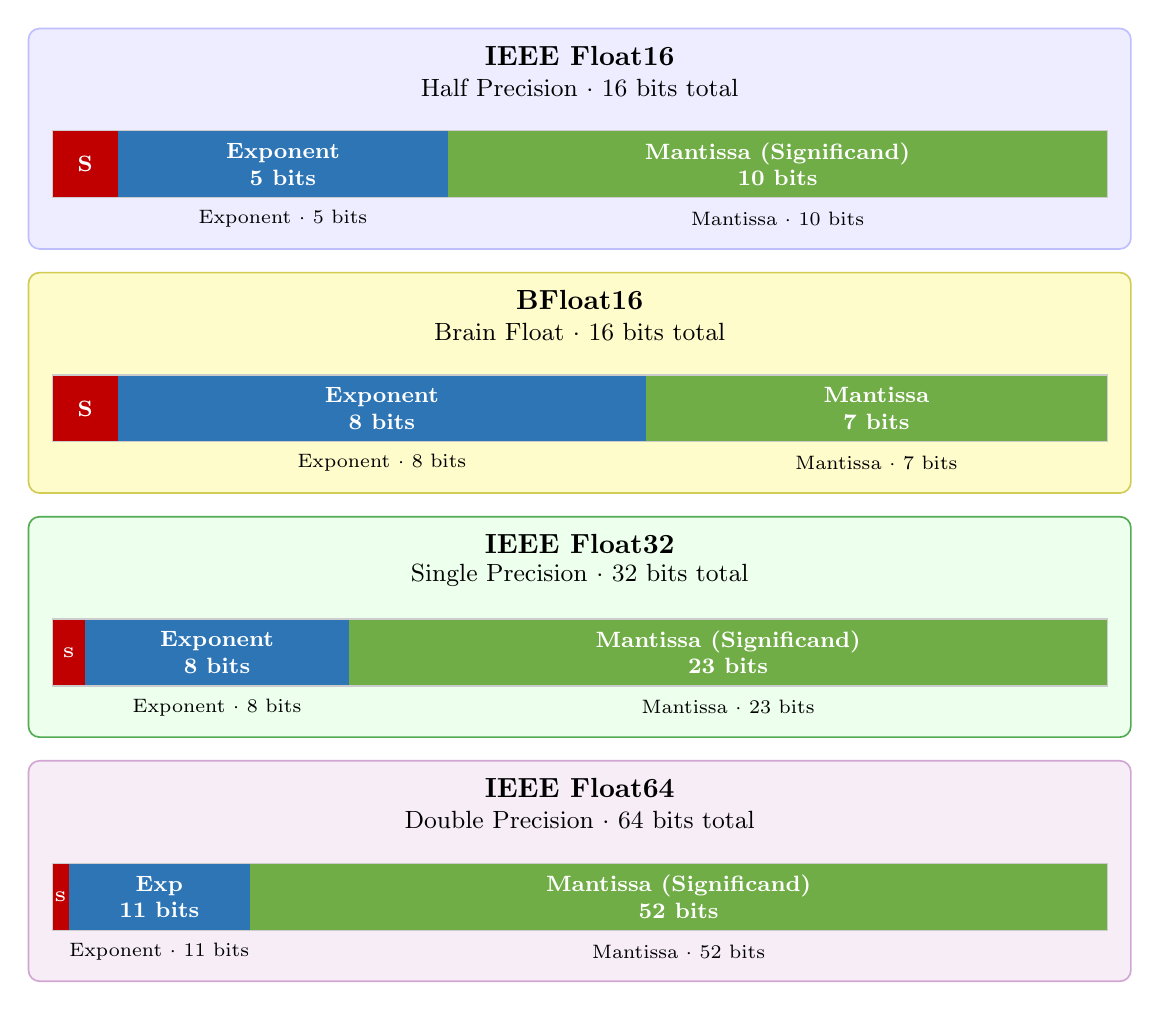
\begin{tikzpicture}[x=1cm, y=1cm]

  % ---- Color palette ----
  \definecolor{signcolor}{RGB}{192,0,0}     % red   -- sign bit
  \definecolor{expcolor} {RGB}{46,117,182}  % blue  -- exponent
  \definecolor{mancolor} {RGB}{112,173,71}  % green -- mantissa

  % ---- Panel backgrounds ----
  % Panels are 14 cm wide x 2.8 cm tall, separated by 0.3 cm gaps.
  % Y positions (bottom edge): Float16=9.30, BFloat16=6.20, Float32=3.10, Float64=0.00
  \draw[rounded corners=4pt, fill=blue!7,    draw=blue!25,        line width=0.6pt]
      (0.0,  9.30) rectangle (14.0, 12.10);  % Float16
  \draw[rounded corners=4pt, fill=yellow!20, draw=yellow!60!gray, line width=0.6pt]
      (0.0,  6.20) rectangle (14.0,  9.00);  % BFloat16
  \draw[rounded corners=4pt, fill=green!7,   draw=green!35!gray,  line width=0.6pt]
      (0.0,  3.10) rectangle (14.0,  5.90);  % Float32
  \draw[rounded corners=4pt, fill=violet!7,  draw=violet!35,      line width=0.6pt]
      (0.0,  0.00) rectangle (14.0,  2.80);  % Float64

  % ====================================================================
  % Bar geometry (shared across all panels):
  %   x range:    [0.30, 13.70]  => total bar width = 13.40 cm
  %   bar height: 0.85 cm
  %   bar bottom: panel_bottom + 0.65
  %   bar top:    panel_bottom + 1.50
  %
  % Segment x boundaries  (width = n_bits/total * 13.40):
  %   Float16  (16-bit): 0.300 | 1.138 | 5.325 | 13.700
  %   BFloat16 (16-bit): 0.300 | 1.138 | 7.838 | 13.700
  %   Float32  (32-bit): 0.300 | 0.719 | 4.069 | 13.700
  %   Float64  (64-bit): 0.300 | 0.509 | 2.813 | 13.700
  % ====================================================================

  % ------------------------------------------------------------------
  % IEEE Float16  (panel bottom y = 9.30)
  % ------------------------------------------------------------------
  \node[font=\normalsize\bfseries] at (7.0, 11.75) {IEEE Float16};
  \node[font=\small]               at (7.0, 11.35) {Half Precision $\cdot$ 16 bits total};

  % S:   1/16 * 13.40 = 0.838 cm   x: 0.300 -- 1.138,  center: 0.719
  \fill[signcolor] (0.300,  9.95) rectangle ( 1.138, 10.80);
  \node[text=white, font=\footnotesize\bfseries] at (0.719, 10.375) {S};

  % Exp: 5/16 * 13.40 = 4.188 cm   x: 1.138 -- 5.325,  center: 3.231
  \fill[expcolor]  (1.138,  9.95) rectangle ( 5.325, 10.80);
  \node[text=white, font=\footnotesize\bfseries, align=center] at (3.231, 10.375)
      {Exponent \\ 5 bits};

  % Man: 10/16 * 13.40 = 8.375 cm  x: 5.325 -- 13.700, center: 9.513
  \fill[mancolor]  (5.325,  9.95) rectangle (13.700, 10.80);
  \node[text=white, font=\footnotesize\bfseries, align=center] at (9.513, 10.375)
      {Mantissa (Significand) \\ 10 bits};

  \draw[black!20, line width=0.4pt] (0.300, 9.95) rectangle (13.700, 10.80);

  \node[font=\scriptsize] at (3.231, 9.68) {Exponent $\cdot$ 5 bits};
  \node[font=\scriptsize] at (9.513, 9.68) {Mantissa $\cdot$ 10 bits};

  % ------------------------------------------------------------------
  % BFloat16  (panel bottom y = 6.20)
  % ------------------------------------------------------------------
  \node[font=\normalsize\bfseries] at (7.0, 8.65) {BFloat16};
  \node[font=\small]               at (7.0, 8.25) {Brain Float $\cdot$ 16 bits total};

  % S:   1/16 * 13.40 = 0.838 cm   x: 0.300 -- 1.138,  center: 0.719
  \fill[signcolor] (0.300,  6.85) rectangle ( 1.138,  7.70);
  \node[text=white, font=\footnotesize\bfseries] at (0.719, 7.275) {S};

  % Exp: 8/16 * 13.40 = 6.700 cm   x: 1.138 -- 7.838,  center: 4.488
  \fill[expcolor]  (1.138,  6.85) rectangle ( 7.838,  7.70);
  \node[text=white, font=\footnotesize\bfseries, align=center] at (4.488, 7.275)
      {Exponent \\ 8 bits};

  % Man: 7/16 * 13.40 = 5.863 cm   x: 7.838 -- 13.700, center: 10.769
  \fill[mancolor]  (7.838,  6.85) rectangle (13.700,  7.70);
  \node[text=white, font=\footnotesize\bfseries, align=center] at (10.769, 7.275)
      {Mantissa \\ 7 bits};

  \draw[black!20, line width=0.4pt] (0.300, 6.85) rectangle (13.700, 7.70);

  \node[font=\scriptsize] at ( 4.488, 6.58) {Exponent $\cdot$ 8 bits};
  \node[font=\scriptsize] at (10.769, 6.58) {Mantissa $\cdot$ 7 bits};

  % ------------------------------------------------------------------
  % IEEE Float32  (panel bottom y = 3.10)
  % ------------------------------------------------------------------
  \node[font=\normalsize\bfseries] at (7.0, 5.55) {IEEE Float32};
  \node[font=\small]               at (7.0, 5.15) {Single Precision $\cdot$ 32 bits total};

  % S:   1/32 * 13.40 = 0.419 cm   x: 0.300 -- 0.719,  center: 0.510
  \fill[signcolor] (0.300,  3.75) rectangle ( 0.719,  4.60);
  \node[text=white, font=\tiny\bfseries] at (0.510, 4.175) {S};

  % Exp: 8/32 * 13.40 = 3.350 cm   x: 0.719 -- 4.069,  center: 2.394
  \fill[expcolor]  (0.719,  3.75) rectangle ( 4.069,  4.60);
  \node[text=white, font=\footnotesize\bfseries, align=center] at (2.394, 4.175)
      {Exponent \\ 8 bits};

  % Man: 23/32 * 13.40 = 9.631 cm  x: 4.069 -- 13.700, center: 8.885
  \fill[mancolor]  (4.069,  3.75) rectangle (13.700,  4.60);
  \node[text=white, font=\footnotesize\bfseries, align=center] at (8.885, 4.175)
      {Mantissa (Significand) \\ 23 bits};

  \draw[black!20, line width=0.4pt] (0.300, 3.75) rectangle (13.700, 4.60);

  \node[font=\scriptsize] at (2.394, 3.48) {Exponent $\cdot$ 8 bits};
  \node[font=\scriptsize] at (8.885, 3.48) {Mantissa $\cdot$ 23 bits};

  % ------------------------------------------------------------------
  % IEEE Float64  (panel bottom y = 0.00)
  % ------------------------------------------------------------------
  \node[font=\normalsize\bfseries] at (7.0, 2.45) {IEEE Float64};
  \node[font=\small]               at (7.0, 2.05) {Double Precision $\cdot$ 64 bits total};

  % S:    1/64 * 13.40 = 0.209 cm  x: 0.300 -- 0.509,  center: 0.405
  \fill[signcolor] (0.300,  0.65) rectangle ( 0.509,  1.50);
  \node[text=white, font=\tiny\bfseries] at (0.405, 1.075) {S};

  % Exp: 11/64 * 13.40 = 2.303 cm  x: 0.509 -- 2.813,  center: 1.661
  \fill[expcolor]  (0.509,  0.65) rectangle ( 2.813,  1.50);
  \node[text=white, font=\footnotesize\bfseries, align=center] at (1.661, 1.075)
      {Exp \\ 11 bits};

  % Man: 52/64 * 13.40 = 10.888 cm x: 2.813 -- 13.700, center: 8.257
  \fill[mancolor]  (2.813,  0.65) rectangle (13.700,  1.50);
  \node[text=white, font=\footnotesize\bfseries, align=center] at (8.257, 1.075)
      {Mantissa (Significand) \\ 52 bits};

  \draw[black!20, line width=0.4pt] (0.300, 0.65) rectangle (13.700, 1.50);

  \node[font=\scriptsize] at (1.661, 0.38) {Exponent $\cdot$ 11 bits};
  \node[font=\scriptsize] at (8.257, 0.38) {Mantissa $\cdot$ 52 bits};

\end{tikzpicture}
}
%
%   Fit to the full page width (~17.8 cm in IEEE two-column):
%     \resizebox{\textwidth}{!}{% Floating-point format comparison — single-column stack layout
%
% Required in preamble:
%   \usepackage{tikz}
%
% ---- Scaling -------------------------------------------------------
% The tikzpicture is drawn at its natural size: 14 cm wide x 12.1 cm tall.
% Use \resizebox (from the graphicx package, always loaded in IEEE style)
% to scale it to whatever width you need. The height adjusts automatically.
%
%   Fit to a single text column (~8.8 cm in IEEE two-column):
%     \resizebox{\columnwidth}{!}{\input{float_formats_tikz.tex}}
%
%   Fit to the full page width (~17.8 cm in IEEE two-column):
%     \resizebox{\textwidth}{!}{\input{float_formats_tikz.tex}}
%
%   Fit to an arbitrary fraction of the column width:
%     \resizebox{0.9\columnwidth}{!}{\input{float_formats_tikz.tex}}
%
% \resizebox scales everything uniformly — coordinates, line widths,
% and fonts — so the result looks identical regardless of the chosen width.
%
% Recommended figure wrapper (single column):
%   \begin{figure}[t]
%     \centering
%     \resizebox{\columnwidth}{!}{\input{float_formats_tikz.tex}}
%     \caption{...}
%     \label{fig:float-formats}
%   \end{figure}
% --------------------------------------------------------------------
%
% Layout: 4 panels stacked vertically, each 14 cm x 2.8 cm.
% Bar widths are proportional to actual bit-field widths.
%   Float16:  S=1, Exp=5,  Man=10  (16 bits total)
%   BFloat16: S=1, Exp=8,  Man=7   (16 bits total)
%   Float32:  S=1, Exp=8,  Man=23  (32 bits total)
%   Float64:  S=1, Exp=11, Man=52  (64 bits total)

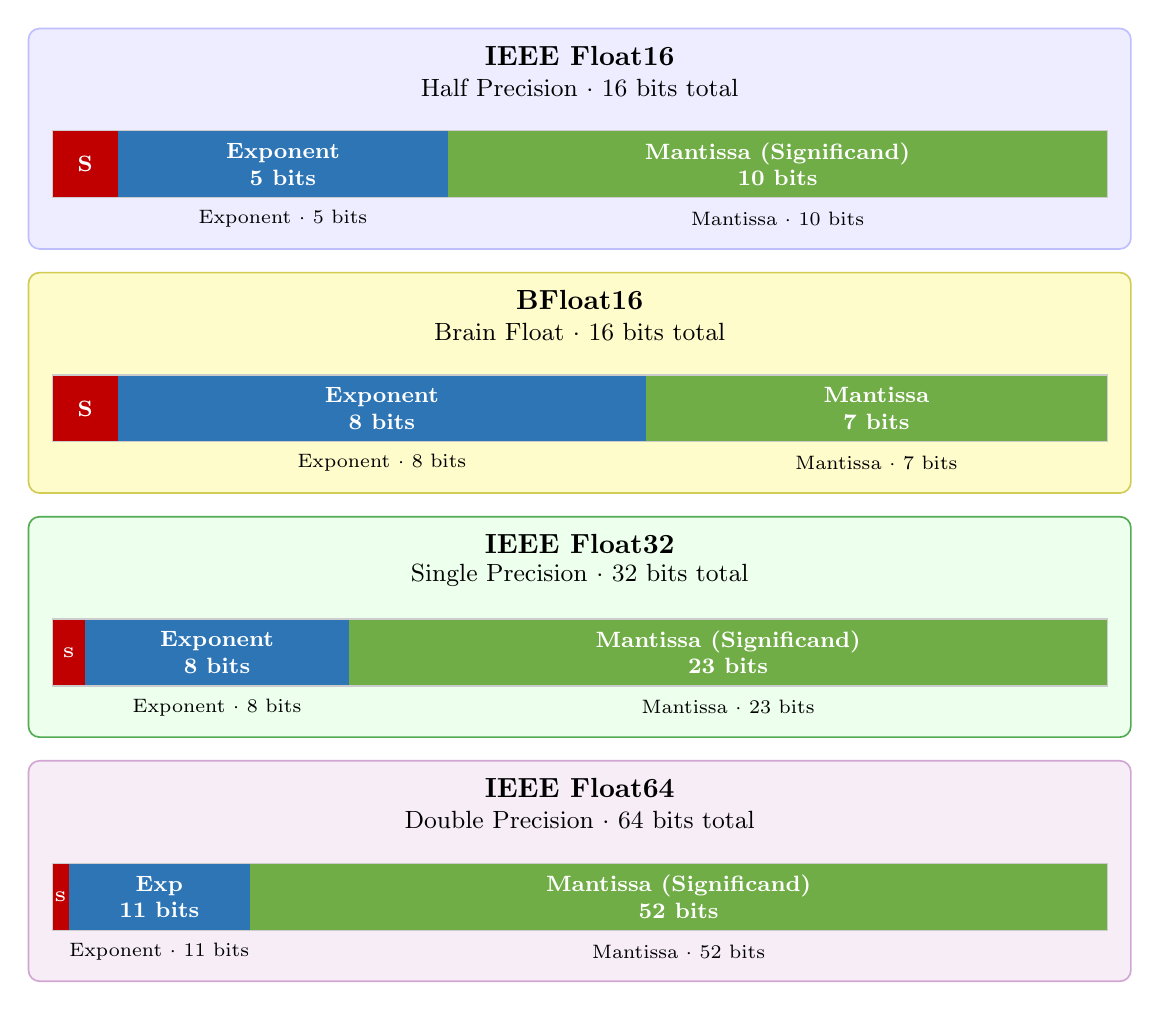
\begin{tikzpicture}[x=1cm, y=1cm]

  % ---- Color palette ----
  \definecolor{signcolor}{RGB}{192,0,0}     % red   -- sign bit
  \definecolor{expcolor} {RGB}{46,117,182}  % blue  -- exponent
  \definecolor{mancolor} {RGB}{112,173,71}  % green -- mantissa

  % ---- Panel backgrounds ----
  % Panels are 14 cm wide x 2.8 cm tall, separated by 0.3 cm gaps.
  % Y positions (bottom edge): Float16=9.30, BFloat16=6.20, Float32=3.10, Float64=0.00
  \draw[rounded corners=4pt, fill=blue!7,    draw=blue!25,        line width=0.6pt]
      (0.0,  9.30) rectangle (14.0, 12.10);  % Float16
  \draw[rounded corners=4pt, fill=yellow!20, draw=yellow!60!gray, line width=0.6pt]
      (0.0,  6.20) rectangle (14.0,  9.00);  % BFloat16
  \draw[rounded corners=4pt, fill=green!7,   draw=green!35!gray,  line width=0.6pt]
      (0.0,  3.10) rectangle (14.0,  5.90);  % Float32
  \draw[rounded corners=4pt, fill=violet!7,  draw=violet!35,      line width=0.6pt]
      (0.0,  0.00) rectangle (14.0,  2.80);  % Float64

  % ====================================================================
  % Bar geometry (shared across all panels):
  %   x range:    [0.30, 13.70]  => total bar width = 13.40 cm
  %   bar height: 0.85 cm
  %   bar bottom: panel_bottom + 0.65
  %   bar top:    panel_bottom + 1.50
  %
  % Segment x boundaries  (width = n_bits/total * 13.40):
  %   Float16  (16-bit): 0.300 | 1.138 | 5.325 | 13.700
  %   BFloat16 (16-bit): 0.300 | 1.138 | 7.838 | 13.700
  %   Float32  (32-bit): 0.300 | 0.719 | 4.069 | 13.700
  %   Float64  (64-bit): 0.300 | 0.509 | 2.813 | 13.700
  % ====================================================================

  % ------------------------------------------------------------------
  % IEEE Float16  (panel bottom y = 9.30)
  % ------------------------------------------------------------------
  \node[font=\normalsize\bfseries] at (7.0, 11.75) {IEEE Float16};
  \node[font=\small]               at (7.0, 11.35) {Half Precision $\cdot$ 16 bits total};

  % S:   1/16 * 13.40 = 0.838 cm   x: 0.300 -- 1.138,  center: 0.719
  \fill[signcolor] (0.300,  9.95) rectangle ( 1.138, 10.80);
  \node[text=white, font=\footnotesize\bfseries] at (0.719, 10.375) {S};

  % Exp: 5/16 * 13.40 = 4.188 cm   x: 1.138 -- 5.325,  center: 3.231
  \fill[expcolor]  (1.138,  9.95) rectangle ( 5.325, 10.80);
  \node[text=white, font=\footnotesize\bfseries, align=center] at (3.231, 10.375)
      {Exponent \\ 5 bits};

  % Man: 10/16 * 13.40 = 8.375 cm  x: 5.325 -- 13.700, center: 9.513
  \fill[mancolor]  (5.325,  9.95) rectangle (13.700, 10.80);
  \node[text=white, font=\footnotesize\bfseries, align=center] at (9.513, 10.375)
      {Mantissa (Significand) \\ 10 bits};

  \draw[black!20, line width=0.4pt] (0.300, 9.95) rectangle (13.700, 10.80);

  \node[font=\scriptsize] at (3.231, 9.68) {Exponent $\cdot$ 5 bits};
  \node[font=\scriptsize] at (9.513, 9.68) {Mantissa $\cdot$ 10 bits};

  % ------------------------------------------------------------------
  % BFloat16  (panel bottom y = 6.20)
  % ------------------------------------------------------------------
  \node[font=\normalsize\bfseries] at (7.0, 8.65) {BFloat16};
  \node[font=\small]               at (7.0, 8.25) {Brain Float $\cdot$ 16 bits total};

  % S:   1/16 * 13.40 = 0.838 cm   x: 0.300 -- 1.138,  center: 0.719
  \fill[signcolor] (0.300,  6.85) rectangle ( 1.138,  7.70);
  \node[text=white, font=\footnotesize\bfseries] at (0.719, 7.275) {S};

  % Exp: 8/16 * 13.40 = 6.700 cm   x: 1.138 -- 7.838,  center: 4.488
  \fill[expcolor]  (1.138,  6.85) rectangle ( 7.838,  7.70);
  \node[text=white, font=\footnotesize\bfseries, align=center] at (4.488, 7.275)
      {Exponent \\ 8 bits};

  % Man: 7/16 * 13.40 = 5.863 cm   x: 7.838 -- 13.700, center: 10.769
  \fill[mancolor]  (7.838,  6.85) rectangle (13.700,  7.70);
  \node[text=white, font=\footnotesize\bfseries, align=center] at (10.769, 7.275)
      {Mantissa \\ 7 bits};

  \draw[black!20, line width=0.4pt] (0.300, 6.85) rectangle (13.700, 7.70);

  \node[font=\scriptsize] at ( 4.488, 6.58) {Exponent $\cdot$ 8 bits};
  \node[font=\scriptsize] at (10.769, 6.58) {Mantissa $\cdot$ 7 bits};

  % ------------------------------------------------------------------
  % IEEE Float32  (panel bottom y = 3.10)
  % ------------------------------------------------------------------
  \node[font=\normalsize\bfseries] at (7.0, 5.55) {IEEE Float32};
  \node[font=\small]               at (7.0, 5.15) {Single Precision $\cdot$ 32 bits total};

  % S:   1/32 * 13.40 = 0.419 cm   x: 0.300 -- 0.719,  center: 0.510
  \fill[signcolor] (0.300,  3.75) rectangle ( 0.719,  4.60);
  \node[text=white, font=\tiny\bfseries] at (0.510, 4.175) {S};

  % Exp: 8/32 * 13.40 = 3.350 cm   x: 0.719 -- 4.069,  center: 2.394
  \fill[expcolor]  (0.719,  3.75) rectangle ( 4.069,  4.60);
  \node[text=white, font=\footnotesize\bfseries, align=center] at (2.394, 4.175)
      {Exponent \\ 8 bits};

  % Man: 23/32 * 13.40 = 9.631 cm  x: 4.069 -- 13.700, center: 8.885
  \fill[mancolor]  (4.069,  3.75) rectangle (13.700,  4.60);
  \node[text=white, font=\footnotesize\bfseries, align=center] at (8.885, 4.175)
      {Mantissa (Significand) \\ 23 bits};

  \draw[black!20, line width=0.4pt] (0.300, 3.75) rectangle (13.700, 4.60);

  \node[font=\scriptsize] at (2.394, 3.48) {Exponent $\cdot$ 8 bits};
  \node[font=\scriptsize] at (8.885, 3.48) {Mantissa $\cdot$ 23 bits};

  % ------------------------------------------------------------------
  % IEEE Float64  (panel bottom y = 0.00)
  % ------------------------------------------------------------------
  \node[font=\normalsize\bfseries] at (7.0, 2.45) {IEEE Float64};
  \node[font=\small]               at (7.0, 2.05) {Double Precision $\cdot$ 64 bits total};

  % S:    1/64 * 13.40 = 0.209 cm  x: 0.300 -- 0.509,  center: 0.405
  \fill[signcolor] (0.300,  0.65) rectangle ( 0.509,  1.50);
  \node[text=white, font=\tiny\bfseries] at (0.405, 1.075) {S};

  % Exp: 11/64 * 13.40 = 2.303 cm  x: 0.509 -- 2.813,  center: 1.661
  \fill[expcolor]  (0.509,  0.65) rectangle ( 2.813,  1.50);
  \node[text=white, font=\footnotesize\bfseries, align=center] at (1.661, 1.075)
      {Exp \\ 11 bits};

  % Man: 52/64 * 13.40 = 10.888 cm x: 2.813 -- 13.700, center: 8.257
  \fill[mancolor]  (2.813,  0.65) rectangle (13.700,  1.50);
  \node[text=white, font=\footnotesize\bfseries, align=center] at (8.257, 1.075)
      {Mantissa (Significand) \\ 52 bits};

  \draw[black!20, line width=0.4pt] (0.300, 0.65) rectangle (13.700, 1.50);

  \node[font=\scriptsize] at (1.661, 0.38) {Exponent $\cdot$ 11 bits};
  \node[font=\scriptsize] at (8.257, 0.38) {Mantissa $\cdot$ 52 bits};

\end{tikzpicture}
}
%
%   Fit to an arbitrary fraction of the column width:
%     \resizebox{0.9\columnwidth}{!}{% Floating-point format comparison — single-column stack layout
%
% Required in preamble:
%   \usepackage{tikz}
%
% ---- Scaling -------------------------------------------------------
% The tikzpicture is drawn at its natural size: 14 cm wide x 12.1 cm tall.
% Use \resizebox (from the graphicx package, always loaded in IEEE style)
% to scale it to whatever width you need. The height adjusts automatically.
%
%   Fit to a single text column (~8.8 cm in IEEE two-column):
%     \resizebox{\columnwidth}{!}{\input{float_formats_tikz.tex}}
%
%   Fit to the full page width (~17.8 cm in IEEE two-column):
%     \resizebox{\textwidth}{!}{\input{float_formats_tikz.tex}}
%
%   Fit to an arbitrary fraction of the column width:
%     \resizebox{0.9\columnwidth}{!}{\input{float_formats_tikz.tex}}
%
% \resizebox scales everything uniformly — coordinates, line widths,
% and fonts — so the result looks identical regardless of the chosen width.
%
% Recommended figure wrapper (single column):
%   \begin{figure}[t]
%     \centering
%     \resizebox{\columnwidth}{!}{\input{float_formats_tikz.tex}}
%     \caption{...}
%     \label{fig:float-formats}
%   \end{figure}
% --------------------------------------------------------------------
%
% Layout: 4 panels stacked vertically, each 14 cm x 2.8 cm.
% Bar widths are proportional to actual bit-field widths.
%   Float16:  S=1, Exp=5,  Man=10  (16 bits total)
%   BFloat16: S=1, Exp=8,  Man=7   (16 bits total)
%   Float32:  S=1, Exp=8,  Man=23  (32 bits total)
%   Float64:  S=1, Exp=11, Man=52  (64 bits total)

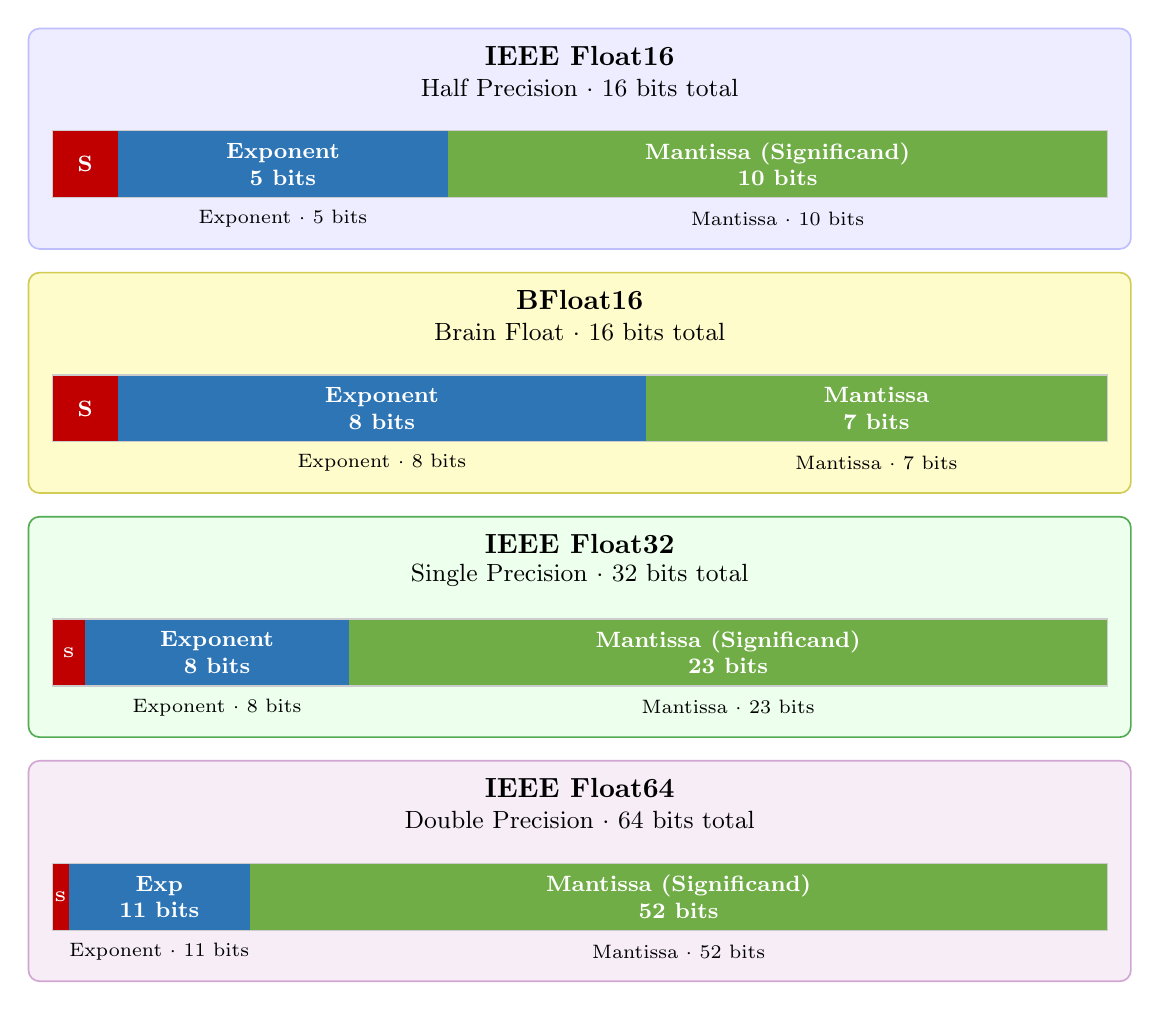
\begin{tikzpicture}[x=1cm, y=1cm]

  % ---- Color palette ----
  \definecolor{signcolor}{RGB}{192,0,0}     % red   -- sign bit
  \definecolor{expcolor} {RGB}{46,117,182}  % blue  -- exponent
  \definecolor{mancolor} {RGB}{112,173,71}  % green -- mantissa

  % ---- Panel backgrounds ----
  % Panels are 14 cm wide x 2.8 cm tall, separated by 0.3 cm gaps.
  % Y positions (bottom edge): Float16=9.30, BFloat16=6.20, Float32=3.10, Float64=0.00
  \draw[rounded corners=4pt, fill=blue!7,    draw=blue!25,        line width=0.6pt]
      (0.0,  9.30) rectangle (14.0, 12.10);  % Float16
  \draw[rounded corners=4pt, fill=yellow!20, draw=yellow!60!gray, line width=0.6pt]
      (0.0,  6.20) rectangle (14.0,  9.00);  % BFloat16
  \draw[rounded corners=4pt, fill=green!7,   draw=green!35!gray,  line width=0.6pt]
      (0.0,  3.10) rectangle (14.0,  5.90);  % Float32
  \draw[rounded corners=4pt, fill=violet!7,  draw=violet!35,      line width=0.6pt]
      (0.0,  0.00) rectangle (14.0,  2.80);  % Float64

  % ====================================================================
  % Bar geometry (shared across all panels):
  %   x range:    [0.30, 13.70]  => total bar width = 13.40 cm
  %   bar height: 0.85 cm
  %   bar bottom: panel_bottom + 0.65
  %   bar top:    panel_bottom + 1.50
  %
  % Segment x boundaries  (width = n_bits/total * 13.40):
  %   Float16  (16-bit): 0.300 | 1.138 | 5.325 | 13.700
  %   BFloat16 (16-bit): 0.300 | 1.138 | 7.838 | 13.700
  %   Float32  (32-bit): 0.300 | 0.719 | 4.069 | 13.700
  %   Float64  (64-bit): 0.300 | 0.509 | 2.813 | 13.700
  % ====================================================================

  % ------------------------------------------------------------------
  % IEEE Float16  (panel bottom y = 9.30)
  % ------------------------------------------------------------------
  \node[font=\normalsize\bfseries] at (7.0, 11.75) {IEEE Float16};
  \node[font=\small]               at (7.0, 11.35) {Half Precision $\cdot$ 16 bits total};

  % S:   1/16 * 13.40 = 0.838 cm   x: 0.300 -- 1.138,  center: 0.719
  \fill[signcolor] (0.300,  9.95) rectangle ( 1.138, 10.80);
  \node[text=white, font=\footnotesize\bfseries] at (0.719, 10.375) {S};

  % Exp: 5/16 * 13.40 = 4.188 cm   x: 1.138 -- 5.325,  center: 3.231
  \fill[expcolor]  (1.138,  9.95) rectangle ( 5.325, 10.80);
  \node[text=white, font=\footnotesize\bfseries, align=center] at (3.231, 10.375)
      {Exponent \\ 5 bits};

  % Man: 10/16 * 13.40 = 8.375 cm  x: 5.325 -- 13.700, center: 9.513
  \fill[mancolor]  (5.325,  9.95) rectangle (13.700, 10.80);
  \node[text=white, font=\footnotesize\bfseries, align=center] at (9.513, 10.375)
      {Mantissa (Significand) \\ 10 bits};

  \draw[black!20, line width=0.4pt] (0.300, 9.95) rectangle (13.700, 10.80);

  \node[font=\scriptsize] at (3.231, 9.68) {Exponent $\cdot$ 5 bits};
  \node[font=\scriptsize] at (9.513, 9.68) {Mantissa $\cdot$ 10 bits};

  % ------------------------------------------------------------------
  % BFloat16  (panel bottom y = 6.20)
  % ------------------------------------------------------------------
  \node[font=\normalsize\bfseries] at (7.0, 8.65) {BFloat16};
  \node[font=\small]               at (7.0, 8.25) {Brain Float $\cdot$ 16 bits total};

  % S:   1/16 * 13.40 = 0.838 cm   x: 0.300 -- 1.138,  center: 0.719
  \fill[signcolor] (0.300,  6.85) rectangle ( 1.138,  7.70);
  \node[text=white, font=\footnotesize\bfseries] at (0.719, 7.275) {S};

  % Exp: 8/16 * 13.40 = 6.700 cm   x: 1.138 -- 7.838,  center: 4.488
  \fill[expcolor]  (1.138,  6.85) rectangle ( 7.838,  7.70);
  \node[text=white, font=\footnotesize\bfseries, align=center] at (4.488, 7.275)
      {Exponent \\ 8 bits};

  % Man: 7/16 * 13.40 = 5.863 cm   x: 7.838 -- 13.700, center: 10.769
  \fill[mancolor]  (7.838,  6.85) rectangle (13.700,  7.70);
  \node[text=white, font=\footnotesize\bfseries, align=center] at (10.769, 7.275)
      {Mantissa \\ 7 bits};

  \draw[black!20, line width=0.4pt] (0.300, 6.85) rectangle (13.700, 7.70);

  \node[font=\scriptsize] at ( 4.488, 6.58) {Exponent $\cdot$ 8 bits};
  \node[font=\scriptsize] at (10.769, 6.58) {Mantissa $\cdot$ 7 bits};

  % ------------------------------------------------------------------
  % IEEE Float32  (panel bottom y = 3.10)
  % ------------------------------------------------------------------
  \node[font=\normalsize\bfseries] at (7.0, 5.55) {IEEE Float32};
  \node[font=\small]               at (7.0, 5.15) {Single Precision $\cdot$ 32 bits total};

  % S:   1/32 * 13.40 = 0.419 cm   x: 0.300 -- 0.719,  center: 0.510
  \fill[signcolor] (0.300,  3.75) rectangle ( 0.719,  4.60);
  \node[text=white, font=\tiny\bfseries] at (0.510, 4.175) {S};

  % Exp: 8/32 * 13.40 = 3.350 cm   x: 0.719 -- 4.069,  center: 2.394
  \fill[expcolor]  (0.719,  3.75) rectangle ( 4.069,  4.60);
  \node[text=white, font=\footnotesize\bfseries, align=center] at (2.394, 4.175)
      {Exponent \\ 8 bits};

  % Man: 23/32 * 13.40 = 9.631 cm  x: 4.069 -- 13.700, center: 8.885
  \fill[mancolor]  (4.069,  3.75) rectangle (13.700,  4.60);
  \node[text=white, font=\footnotesize\bfseries, align=center] at (8.885, 4.175)
      {Mantissa (Significand) \\ 23 bits};

  \draw[black!20, line width=0.4pt] (0.300, 3.75) rectangle (13.700, 4.60);

  \node[font=\scriptsize] at (2.394, 3.48) {Exponent $\cdot$ 8 bits};
  \node[font=\scriptsize] at (8.885, 3.48) {Mantissa $\cdot$ 23 bits};

  % ------------------------------------------------------------------
  % IEEE Float64  (panel bottom y = 0.00)
  % ------------------------------------------------------------------
  \node[font=\normalsize\bfseries] at (7.0, 2.45) {IEEE Float64};
  \node[font=\small]               at (7.0, 2.05) {Double Precision $\cdot$ 64 bits total};

  % S:    1/64 * 13.40 = 0.209 cm  x: 0.300 -- 0.509,  center: 0.405
  \fill[signcolor] (0.300,  0.65) rectangle ( 0.509,  1.50);
  \node[text=white, font=\tiny\bfseries] at (0.405, 1.075) {S};

  % Exp: 11/64 * 13.40 = 2.303 cm  x: 0.509 -- 2.813,  center: 1.661
  \fill[expcolor]  (0.509,  0.65) rectangle ( 2.813,  1.50);
  \node[text=white, font=\footnotesize\bfseries, align=center] at (1.661, 1.075)
      {Exp \\ 11 bits};

  % Man: 52/64 * 13.40 = 10.888 cm x: 2.813 -- 13.700, center: 8.257
  \fill[mancolor]  (2.813,  0.65) rectangle (13.700,  1.50);
  \node[text=white, font=\footnotesize\bfseries, align=center] at (8.257, 1.075)
      {Mantissa (Significand) \\ 52 bits};

  \draw[black!20, line width=0.4pt] (0.300, 0.65) rectangle (13.700, 1.50);

  \node[font=\scriptsize] at (1.661, 0.38) {Exponent $\cdot$ 11 bits};
  \node[font=\scriptsize] at (8.257, 0.38) {Mantissa $\cdot$ 52 bits};

\end{tikzpicture}
}
%
% \resizebox scales everything uniformly — coordinates, line widths,
% and fonts — so the result looks identical regardless of the chosen width.
%
% Recommended figure wrapper (single column):
%   \begin{figure}[t]
%     \centering
%     \resizebox{\columnwidth}{!}{% Floating-point format comparison — single-column stack layout
%
% Required in preamble:
%   \usepackage{tikz}
%
% ---- Scaling -------------------------------------------------------
% The tikzpicture is drawn at its natural size: 14 cm wide x 12.1 cm tall.
% Use \resizebox (from the graphicx package, always loaded in IEEE style)
% to scale it to whatever width you need. The height adjusts automatically.
%
%   Fit to a single text column (~8.8 cm in IEEE two-column):
%     \resizebox{\columnwidth}{!}{\input{float_formats_tikz.tex}}
%
%   Fit to the full page width (~17.8 cm in IEEE two-column):
%     \resizebox{\textwidth}{!}{\input{float_formats_tikz.tex}}
%
%   Fit to an arbitrary fraction of the column width:
%     \resizebox{0.9\columnwidth}{!}{\input{float_formats_tikz.tex}}
%
% \resizebox scales everything uniformly — coordinates, line widths,
% and fonts — so the result looks identical regardless of the chosen width.
%
% Recommended figure wrapper (single column):
%   \begin{figure}[t]
%     \centering
%     \resizebox{\columnwidth}{!}{\input{float_formats_tikz.tex}}
%     \caption{...}
%     \label{fig:float-formats}
%   \end{figure}
% --------------------------------------------------------------------
%
% Layout: 4 panels stacked vertically, each 14 cm x 2.8 cm.
% Bar widths are proportional to actual bit-field widths.
%   Float16:  S=1, Exp=5,  Man=10  (16 bits total)
%   BFloat16: S=1, Exp=8,  Man=7   (16 bits total)
%   Float32:  S=1, Exp=8,  Man=23  (32 bits total)
%   Float64:  S=1, Exp=11, Man=52  (64 bits total)

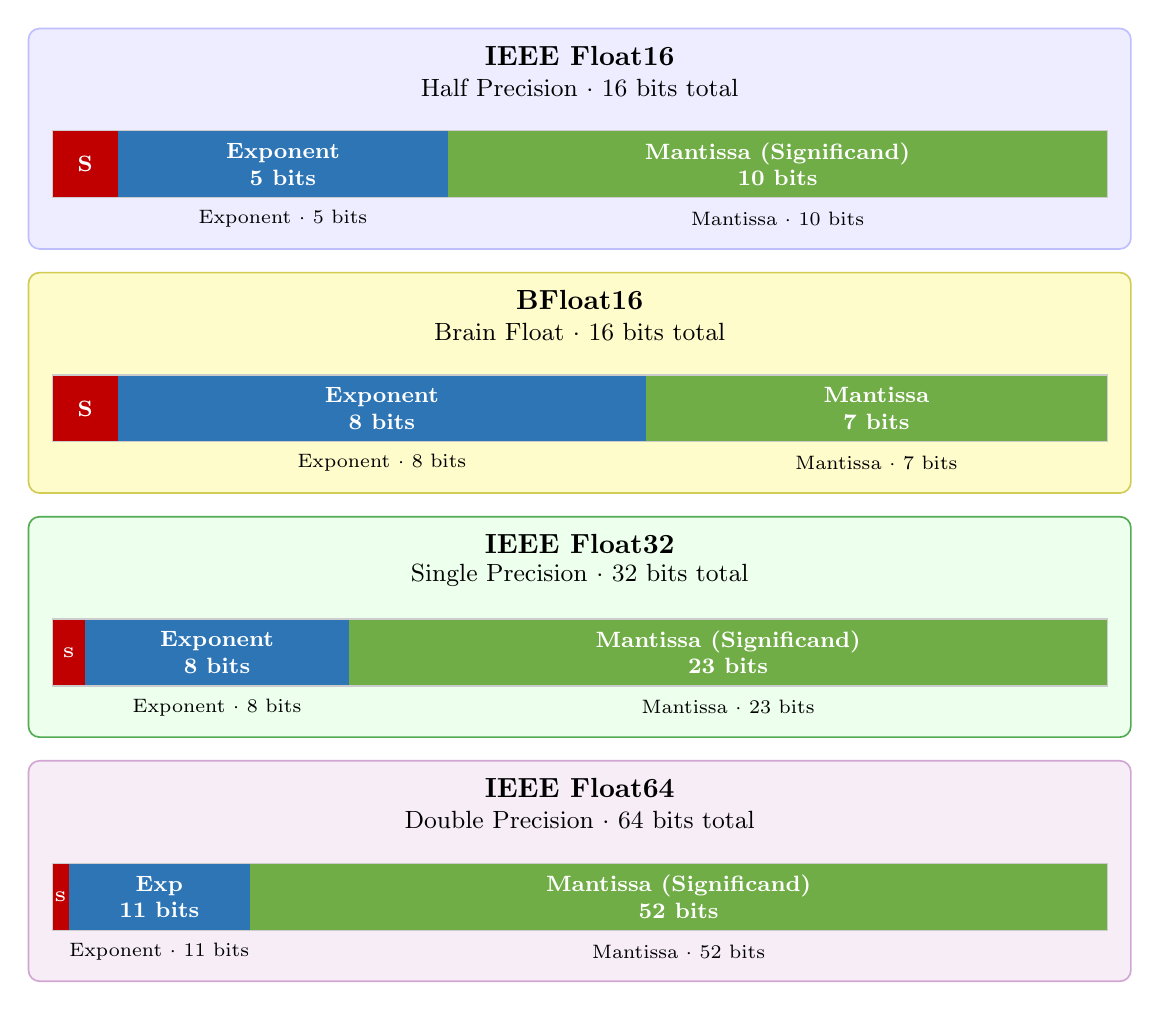
\begin{tikzpicture}[x=1cm, y=1cm]

  % ---- Color palette ----
  \definecolor{signcolor}{RGB}{192,0,0}     % red   -- sign bit
  \definecolor{expcolor} {RGB}{46,117,182}  % blue  -- exponent
  \definecolor{mancolor} {RGB}{112,173,71}  % green -- mantissa

  % ---- Panel backgrounds ----
  % Panels are 14 cm wide x 2.8 cm tall, separated by 0.3 cm gaps.
  % Y positions (bottom edge): Float16=9.30, BFloat16=6.20, Float32=3.10, Float64=0.00
  \draw[rounded corners=4pt, fill=blue!7,    draw=blue!25,        line width=0.6pt]
      (0.0,  9.30) rectangle (14.0, 12.10);  % Float16
  \draw[rounded corners=4pt, fill=yellow!20, draw=yellow!60!gray, line width=0.6pt]
      (0.0,  6.20) rectangle (14.0,  9.00);  % BFloat16
  \draw[rounded corners=4pt, fill=green!7,   draw=green!35!gray,  line width=0.6pt]
      (0.0,  3.10) rectangle (14.0,  5.90);  % Float32
  \draw[rounded corners=4pt, fill=violet!7,  draw=violet!35,      line width=0.6pt]
      (0.0,  0.00) rectangle (14.0,  2.80);  % Float64

  % ====================================================================
  % Bar geometry (shared across all panels):
  %   x range:    [0.30, 13.70]  => total bar width = 13.40 cm
  %   bar height: 0.85 cm
  %   bar bottom: panel_bottom + 0.65
  %   bar top:    panel_bottom + 1.50
  %
  % Segment x boundaries  (width = n_bits/total * 13.40):
  %   Float16  (16-bit): 0.300 | 1.138 | 5.325 | 13.700
  %   BFloat16 (16-bit): 0.300 | 1.138 | 7.838 | 13.700
  %   Float32  (32-bit): 0.300 | 0.719 | 4.069 | 13.700
  %   Float64  (64-bit): 0.300 | 0.509 | 2.813 | 13.700
  % ====================================================================

  % ------------------------------------------------------------------
  % IEEE Float16  (panel bottom y = 9.30)
  % ------------------------------------------------------------------
  \node[font=\normalsize\bfseries] at (7.0, 11.75) {IEEE Float16};
  \node[font=\small]               at (7.0, 11.35) {Half Precision $\cdot$ 16 bits total};

  % S:   1/16 * 13.40 = 0.838 cm   x: 0.300 -- 1.138,  center: 0.719
  \fill[signcolor] (0.300,  9.95) rectangle ( 1.138, 10.80);
  \node[text=white, font=\footnotesize\bfseries] at (0.719, 10.375) {S};

  % Exp: 5/16 * 13.40 = 4.188 cm   x: 1.138 -- 5.325,  center: 3.231
  \fill[expcolor]  (1.138,  9.95) rectangle ( 5.325, 10.80);
  \node[text=white, font=\footnotesize\bfseries, align=center] at (3.231, 10.375)
      {Exponent \\ 5 bits};

  % Man: 10/16 * 13.40 = 8.375 cm  x: 5.325 -- 13.700, center: 9.513
  \fill[mancolor]  (5.325,  9.95) rectangle (13.700, 10.80);
  \node[text=white, font=\footnotesize\bfseries, align=center] at (9.513, 10.375)
      {Mantissa (Significand) \\ 10 bits};

  \draw[black!20, line width=0.4pt] (0.300, 9.95) rectangle (13.700, 10.80);

  \node[font=\scriptsize] at (3.231, 9.68) {Exponent $\cdot$ 5 bits};
  \node[font=\scriptsize] at (9.513, 9.68) {Mantissa $\cdot$ 10 bits};

  % ------------------------------------------------------------------
  % BFloat16  (panel bottom y = 6.20)
  % ------------------------------------------------------------------
  \node[font=\normalsize\bfseries] at (7.0, 8.65) {BFloat16};
  \node[font=\small]               at (7.0, 8.25) {Brain Float $\cdot$ 16 bits total};

  % S:   1/16 * 13.40 = 0.838 cm   x: 0.300 -- 1.138,  center: 0.719
  \fill[signcolor] (0.300,  6.85) rectangle ( 1.138,  7.70);
  \node[text=white, font=\footnotesize\bfseries] at (0.719, 7.275) {S};

  % Exp: 8/16 * 13.40 = 6.700 cm   x: 1.138 -- 7.838,  center: 4.488
  \fill[expcolor]  (1.138,  6.85) rectangle ( 7.838,  7.70);
  \node[text=white, font=\footnotesize\bfseries, align=center] at (4.488, 7.275)
      {Exponent \\ 8 bits};

  % Man: 7/16 * 13.40 = 5.863 cm   x: 7.838 -- 13.700, center: 10.769
  \fill[mancolor]  (7.838,  6.85) rectangle (13.700,  7.70);
  \node[text=white, font=\footnotesize\bfseries, align=center] at (10.769, 7.275)
      {Mantissa \\ 7 bits};

  \draw[black!20, line width=0.4pt] (0.300, 6.85) rectangle (13.700, 7.70);

  \node[font=\scriptsize] at ( 4.488, 6.58) {Exponent $\cdot$ 8 bits};
  \node[font=\scriptsize] at (10.769, 6.58) {Mantissa $\cdot$ 7 bits};

  % ------------------------------------------------------------------
  % IEEE Float32  (panel bottom y = 3.10)
  % ------------------------------------------------------------------
  \node[font=\normalsize\bfseries] at (7.0, 5.55) {IEEE Float32};
  \node[font=\small]               at (7.0, 5.15) {Single Precision $\cdot$ 32 bits total};

  % S:   1/32 * 13.40 = 0.419 cm   x: 0.300 -- 0.719,  center: 0.510
  \fill[signcolor] (0.300,  3.75) rectangle ( 0.719,  4.60);
  \node[text=white, font=\tiny\bfseries] at (0.510, 4.175) {S};

  % Exp: 8/32 * 13.40 = 3.350 cm   x: 0.719 -- 4.069,  center: 2.394
  \fill[expcolor]  (0.719,  3.75) rectangle ( 4.069,  4.60);
  \node[text=white, font=\footnotesize\bfseries, align=center] at (2.394, 4.175)
      {Exponent \\ 8 bits};

  % Man: 23/32 * 13.40 = 9.631 cm  x: 4.069 -- 13.700, center: 8.885
  \fill[mancolor]  (4.069,  3.75) rectangle (13.700,  4.60);
  \node[text=white, font=\footnotesize\bfseries, align=center] at (8.885, 4.175)
      {Mantissa (Significand) \\ 23 bits};

  \draw[black!20, line width=0.4pt] (0.300, 3.75) rectangle (13.700, 4.60);

  \node[font=\scriptsize] at (2.394, 3.48) {Exponent $\cdot$ 8 bits};
  \node[font=\scriptsize] at (8.885, 3.48) {Mantissa $\cdot$ 23 bits};

  % ------------------------------------------------------------------
  % IEEE Float64  (panel bottom y = 0.00)
  % ------------------------------------------------------------------
  \node[font=\normalsize\bfseries] at (7.0, 2.45) {IEEE Float64};
  \node[font=\small]               at (7.0, 2.05) {Double Precision $\cdot$ 64 bits total};

  % S:    1/64 * 13.40 = 0.209 cm  x: 0.300 -- 0.509,  center: 0.405
  \fill[signcolor] (0.300,  0.65) rectangle ( 0.509,  1.50);
  \node[text=white, font=\tiny\bfseries] at (0.405, 1.075) {S};

  % Exp: 11/64 * 13.40 = 2.303 cm  x: 0.509 -- 2.813,  center: 1.661
  \fill[expcolor]  (0.509,  0.65) rectangle ( 2.813,  1.50);
  \node[text=white, font=\footnotesize\bfseries, align=center] at (1.661, 1.075)
      {Exp \\ 11 bits};

  % Man: 52/64 * 13.40 = 10.888 cm x: 2.813 -- 13.700, center: 8.257
  \fill[mancolor]  (2.813,  0.65) rectangle (13.700,  1.50);
  \node[text=white, font=\footnotesize\bfseries, align=center] at (8.257, 1.075)
      {Mantissa (Significand) \\ 52 bits};

  \draw[black!20, line width=0.4pt] (0.300, 0.65) rectangle (13.700, 1.50);

  \node[font=\scriptsize] at (1.661, 0.38) {Exponent $\cdot$ 11 bits};
  \node[font=\scriptsize] at (8.257, 0.38) {Mantissa $\cdot$ 52 bits};

\end{tikzpicture}
}
%     \caption{...}
%     \label{fig:float-formats}
%   \end{figure}
% --------------------------------------------------------------------
%
% Layout: 4 panels stacked vertically, each 14 cm x 2.8 cm.
% Bar widths are proportional to actual bit-field widths.
%   Float16:  S=1, Exp=5,  Man=10  (16 bits total)
%   BFloat16: S=1, Exp=8,  Man=7   (16 bits total)
%   Float32:  S=1, Exp=8,  Man=23  (32 bits total)
%   Float64:  S=1, Exp=11, Man=52  (64 bits total)

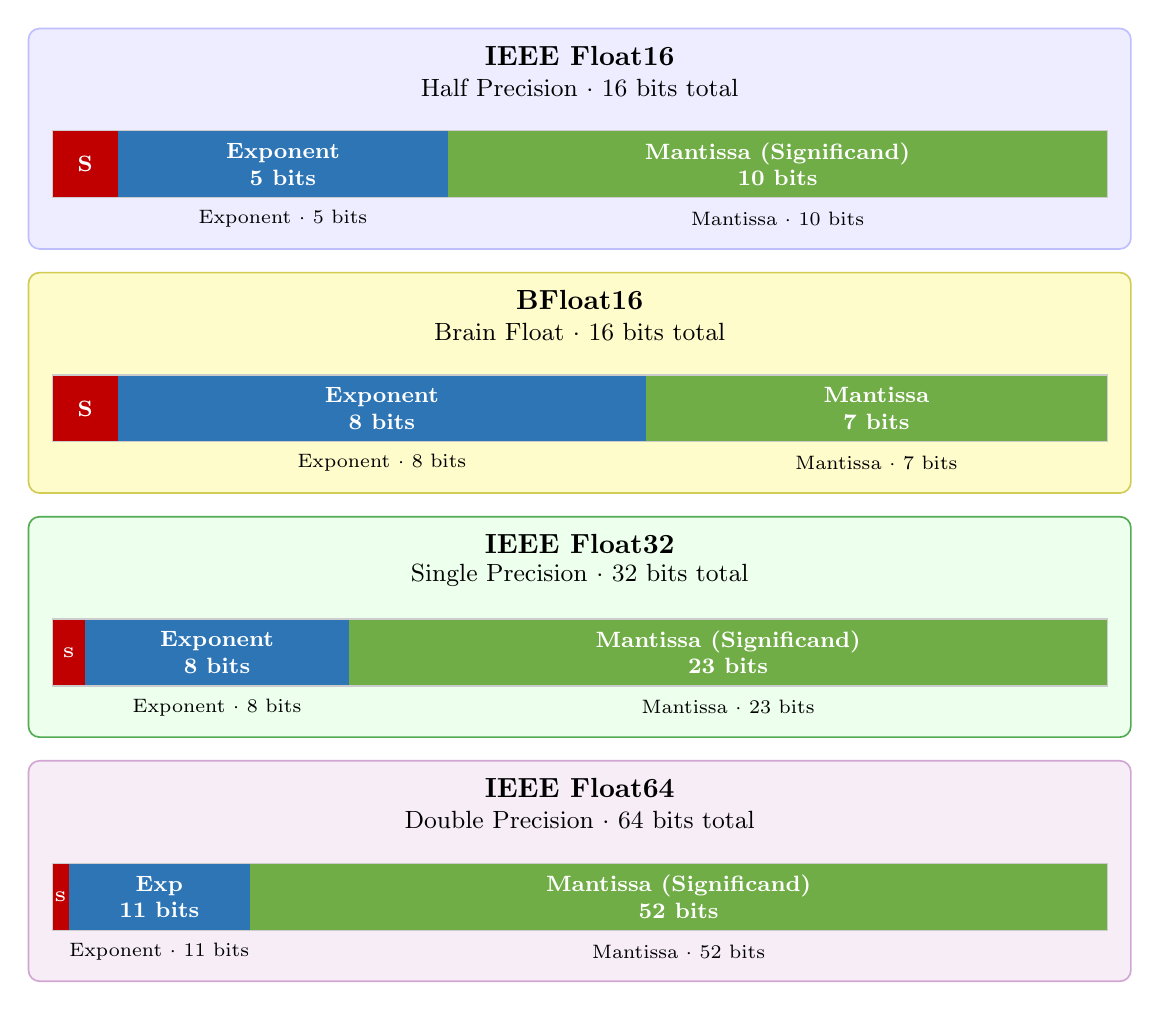
\begin{tikzpicture}[x=1cm, y=1cm]

  % ---- Color palette ----
  \definecolor{signcolor}{RGB}{192,0,0}     % red   -- sign bit
  \definecolor{expcolor} {RGB}{46,117,182}  % blue  -- exponent
  \definecolor{mancolor} {RGB}{112,173,71}  % green -- mantissa

  % ---- Panel backgrounds ----
  % Panels are 14 cm wide x 2.8 cm tall, separated by 0.3 cm gaps.
  % Y positions (bottom edge): Float16=9.30, BFloat16=6.20, Float32=3.10, Float64=0.00
  \draw[rounded corners=4pt, fill=blue!7,    draw=blue!25,        line width=0.6pt]
      (0.0,  9.30) rectangle (14.0, 12.10);  % Float16
  \draw[rounded corners=4pt, fill=yellow!20, draw=yellow!60!gray, line width=0.6pt]
      (0.0,  6.20) rectangle (14.0,  9.00);  % BFloat16
  \draw[rounded corners=4pt, fill=green!7,   draw=green!35!gray,  line width=0.6pt]
      (0.0,  3.10) rectangle (14.0,  5.90);  % Float32
  \draw[rounded corners=4pt, fill=violet!7,  draw=violet!35,      line width=0.6pt]
      (0.0,  0.00) rectangle (14.0,  2.80);  % Float64

  % ====================================================================
  % Bar geometry (shared across all panels):
  %   x range:    [0.30, 13.70]  => total bar width = 13.40 cm
  %   bar height: 0.85 cm
  %   bar bottom: panel_bottom + 0.65
  %   bar top:    panel_bottom + 1.50
  %
  % Segment x boundaries  (width = n_bits/total * 13.40):
  %   Float16  (16-bit): 0.300 | 1.138 | 5.325 | 13.700
  %   BFloat16 (16-bit): 0.300 | 1.138 | 7.838 | 13.700
  %   Float32  (32-bit): 0.300 | 0.719 | 4.069 | 13.700
  %   Float64  (64-bit): 0.300 | 0.509 | 2.813 | 13.700
  % ====================================================================

  % ------------------------------------------------------------------
  % IEEE Float16  (panel bottom y = 9.30)
  % ------------------------------------------------------------------
  \node[font=\normalsize\bfseries] at (7.0, 11.75) {IEEE Float16};
  \node[font=\small]               at (7.0, 11.35) {Half Precision $\cdot$ 16 bits total};

  % S:   1/16 * 13.40 = 0.838 cm   x: 0.300 -- 1.138,  center: 0.719
  \fill[signcolor] (0.300,  9.95) rectangle ( 1.138, 10.80);
  \node[text=white, font=\footnotesize\bfseries] at (0.719, 10.375) {S};

  % Exp: 5/16 * 13.40 = 4.188 cm   x: 1.138 -- 5.325,  center: 3.231
  \fill[expcolor]  (1.138,  9.95) rectangle ( 5.325, 10.80);
  \node[text=white, font=\footnotesize\bfseries, align=center] at (3.231, 10.375)
      {Exponent \\ 5 bits};

  % Man: 10/16 * 13.40 = 8.375 cm  x: 5.325 -- 13.700, center: 9.513
  \fill[mancolor]  (5.325,  9.95) rectangle (13.700, 10.80);
  \node[text=white, font=\footnotesize\bfseries, align=center] at (9.513, 10.375)
      {Mantissa (Significand) \\ 10 bits};

  \draw[black!20, line width=0.4pt] (0.300, 9.95) rectangle (13.700, 10.80);

  \node[font=\scriptsize] at (3.231, 9.68) {Exponent $\cdot$ 5 bits};
  \node[font=\scriptsize] at (9.513, 9.68) {Mantissa $\cdot$ 10 bits};

  % ------------------------------------------------------------------
  % BFloat16  (panel bottom y = 6.20)
  % ------------------------------------------------------------------
  \node[font=\normalsize\bfseries] at (7.0, 8.65) {BFloat16};
  \node[font=\small]               at (7.0, 8.25) {Brain Float $\cdot$ 16 bits total};

  % S:   1/16 * 13.40 = 0.838 cm   x: 0.300 -- 1.138,  center: 0.719
  \fill[signcolor] (0.300,  6.85) rectangle ( 1.138,  7.70);
  \node[text=white, font=\footnotesize\bfseries] at (0.719, 7.275) {S};

  % Exp: 8/16 * 13.40 = 6.700 cm   x: 1.138 -- 7.838,  center: 4.488
  \fill[expcolor]  (1.138,  6.85) rectangle ( 7.838,  7.70);
  \node[text=white, font=\footnotesize\bfseries, align=center] at (4.488, 7.275)
      {Exponent \\ 8 bits};

  % Man: 7/16 * 13.40 = 5.863 cm   x: 7.838 -- 13.700, center: 10.769
  \fill[mancolor]  (7.838,  6.85) rectangle (13.700,  7.70);
  \node[text=white, font=\footnotesize\bfseries, align=center] at (10.769, 7.275)
      {Mantissa \\ 7 bits};

  \draw[black!20, line width=0.4pt] (0.300, 6.85) rectangle (13.700, 7.70);

  \node[font=\scriptsize] at ( 4.488, 6.58) {Exponent $\cdot$ 8 bits};
  \node[font=\scriptsize] at (10.769, 6.58) {Mantissa $\cdot$ 7 bits};

  % ------------------------------------------------------------------
  % IEEE Float32  (panel bottom y = 3.10)
  % ------------------------------------------------------------------
  \node[font=\normalsize\bfseries] at (7.0, 5.55) {IEEE Float32};
  \node[font=\small]               at (7.0, 5.15) {Single Precision $\cdot$ 32 bits total};

  % S:   1/32 * 13.40 = 0.419 cm   x: 0.300 -- 0.719,  center: 0.510
  \fill[signcolor] (0.300,  3.75) rectangle ( 0.719,  4.60);
  \node[text=white, font=\tiny\bfseries] at (0.510, 4.175) {S};

  % Exp: 8/32 * 13.40 = 3.350 cm   x: 0.719 -- 4.069,  center: 2.394
  \fill[expcolor]  (0.719,  3.75) rectangle ( 4.069,  4.60);
  \node[text=white, font=\footnotesize\bfseries, align=center] at (2.394, 4.175)
      {Exponent \\ 8 bits};

  % Man: 23/32 * 13.40 = 9.631 cm  x: 4.069 -- 13.700, center: 8.885
  \fill[mancolor]  (4.069,  3.75) rectangle (13.700,  4.60);
  \node[text=white, font=\footnotesize\bfseries, align=center] at (8.885, 4.175)
      {Mantissa (Significand) \\ 23 bits};

  \draw[black!20, line width=0.4pt] (0.300, 3.75) rectangle (13.700, 4.60);

  \node[font=\scriptsize] at (2.394, 3.48) {Exponent $\cdot$ 8 bits};
  \node[font=\scriptsize] at (8.885, 3.48) {Mantissa $\cdot$ 23 bits};

  % ------------------------------------------------------------------
  % IEEE Float64  (panel bottom y = 0.00)
  % ------------------------------------------------------------------
  \node[font=\normalsize\bfseries] at (7.0, 2.45) {IEEE Float64};
  \node[font=\small]               at (7.0, 2.05) {Double Precision $\cdot$ 64 bits total};

  % S:    1/64 * 13.40 = 0.209 cm  x: 0.300 -- 0.509,  center: 0.405
  \fill[signcolor] (0.300,  0.65) rectangle ( 0.509,  1.50);
  \node[text=white, font=\tiny\bfseries] at (0.405, 1.075) {S};

  % Exp: 11/64 * 13.40 = 2.303 cm  x: 0.509 -- 2.813,  center: 1.661
  \fill[expcolor]  (0.509,  0.65) rectangle ( 2.813,  1.50);
  \node[text=white, font=\footnotesize\bfseries, align=center] at (1.661, 1.075)
      {Exp \\ 11 bits};

  % Man: 52/64 * 13.40 = 10.888 cm x: 2.813 -- 13.700, center: 8.257
  \fill[mancolor]  (2.813,  0.65) rectangle (13.700,  1.50);
  \node[text=white, font=\footnotesize\bfseries, align=center] at (8.257, 1.075)
      {Mantissa (Significand) \\ 52 bits};

  \draw[black!20, line width=0.4pt] (0.300, 0.65) rectangle (13.700, 1.50);

  \node[font=\scriptsize] at (1.661, 0.38) {Exponent $\cdot$ 11 bits};
  \node[font=\scriptsize] at (8.257, 0.38) {Mantissa $\cdot$ 52 bits};

\end{tikzpicture}
}
%
%   Fit to an arbitrary fraction of the column width:
%     \resizebox{0.9\columnwidth}{!}{% Floating-point format comparison — single-column stack layout
%
% Required in preamble:
%   \usepackage{tikz}
%
% ---- Scaling -------------------------------------------------------
% The tikzpicture is drawn at its natural size: 14 cm wide x 12.1 cm tall.
% Use \resizebox (from the graphicx package, always loaded in IEEE style)
% to scale it to whatever width you need. The height adjusts automatically.
%
%   Fit to a single text column (~8.8 cm in IEEE two-column):
%     \resizebox{\columnwidth}{!}{% Floating-point format comparison — single-column stack layout
%
% Required in preamble:
%   \usepackage{tikz}
%
% ---- Scaling -------------------------------------------------------
% The tikzpicture is drawn at its natural size: 14 cm wide x 12.1 cm tall.
% Use \resizebox (from the graphicx package, always loaded in IEEE style)
% to scale it to whatever width you need. The height adjusts automatically.
%
%   Fit to a single text column (~8.8 cm in IEEE two-column):
%     \resizebox{\columnwidth}{!}{\input{float_formats_tikz.tex}}
%
%   Fit to the full page width (~17.8 cm in IEEE two-column):
%     \resizebox{\textwidth}{!}{\input{float_formats_tikz.tex}}
%
%   Fit to an arbitrary fraction of the column width:
%     \resizebox{0.9\columnwidth}{!}{\input{float_formats_tikz.tex}}
%
% \resizebox scales everything uniformly — coordinates, line widths,
% and fonts — so the result looks identical regardless of the chosen width.
%
% Recommended figure wrapper (single column):
%   \begin{figure}[t]
%     \centering
%     \resizebox{\columnwidth}{!}{\input{float_formats_tikz.tex}}
%     \caption{...}
%     \label{fig:float-formats}
%   \end{figure}
% --------------------------------------------------------------------
%
% Layout: 4 panels stacked vertically, each 14 cm x 2.8 cm.
% Bar widths are proportional to actual bit-field widths.
%   Float16:  S=1, Exp=5,  Man=10  (16 bits total)
%   BFloat16: S=1, Exp=8,  Man=7   (16 bits total)
%   Float32:  S=1, Exp=8,  Man=23  (32 bits total)
%   Float64:  S=1, Exp=11, Man=52  (64 bits total)

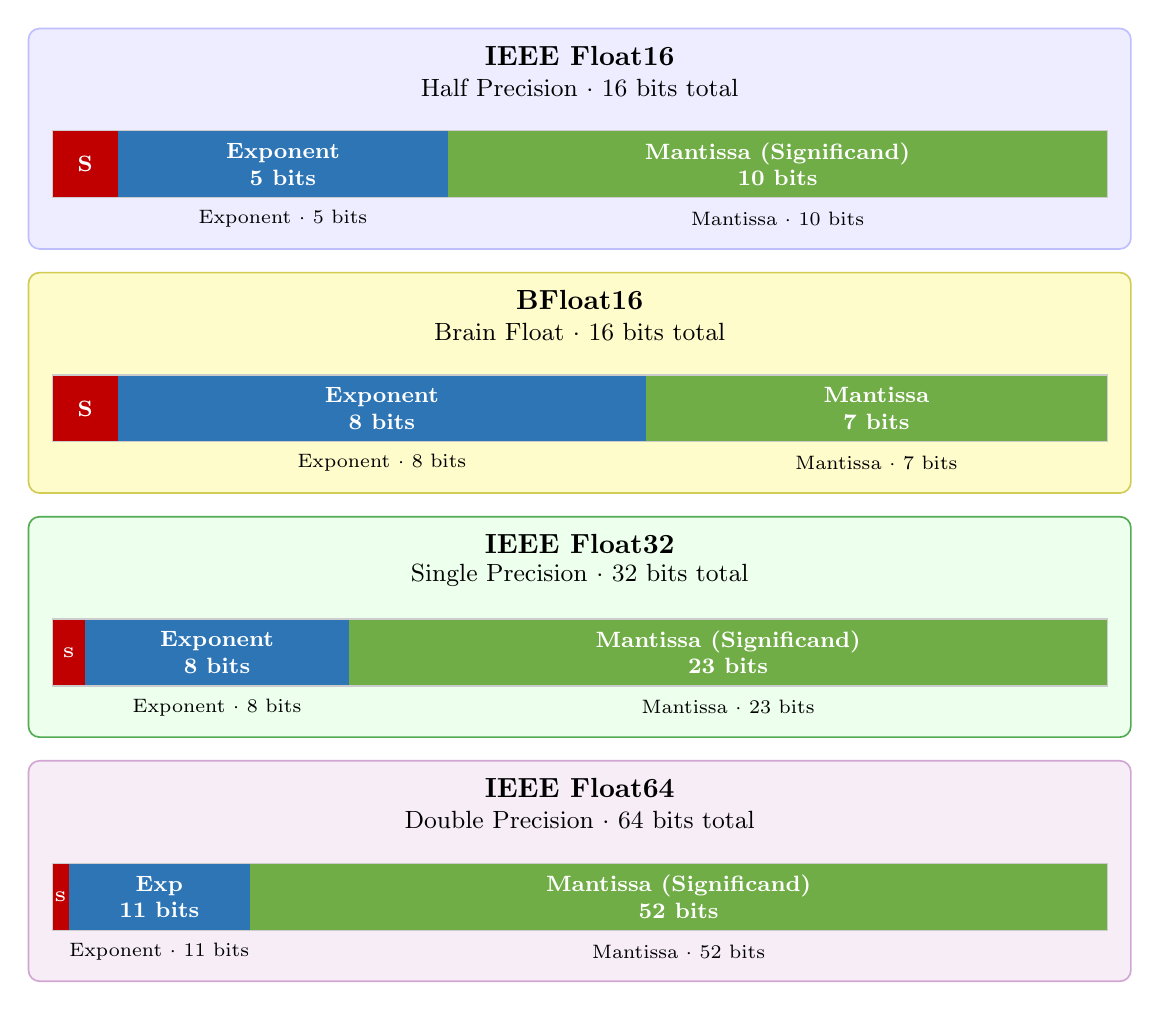
\begin{tikzpicture}[x=1cm, y=1cm]

  % ---- Color palette ----
  \definecolor{signcolor}{RGB}{192,0,0}     % red   -- sign bit
  \definecolor{expcolor} {RGB}{46,117,182}  % blue  -- exponent
  \definecolor{mancolor} {RGB}{112,173,71}  % green -- mantissa

  % ---- Panel backgrounds ----
  % Panels are 14 cm wide x 2.8 cm tall, separated by 0.3 cm gaps.
  % Y positions (bottom edge): Float16=9.30, BFloat16=6.20, Float32=3.10, Float64=0.00
  \draw[rounded corners=4pt, fill=blue!7,    draw=blue!25,        line width=0.6pt]
      (0.0,  9.30) rectangle (14.0, 12.10);  % Float16
  \draw[rounded corners=4pt, fill=yellow!20, draw=yellow!60!gray, line width=0.6pt]
      (0.0,  6.20) rectangle (14.0,  9.00);  % BFloat16
  \draw[rounded corners=4pt, fill=green!7,   draw=green!35!gray,  line width=0.6pt]
      (0.0,  3.10) rectangle (14.0,  5.90);  % Float32
  \draw[rounded corners=4pt, fill=violet!7,  draw=violet!35,      line width=0.6pt]
      (0.0,  0.00) rectangle (14.0,  2.80);  % Float64

  % ====================================================================
  % Bar geometry (shared across all panels):
  %   x range:    [0.30, 13.70]  => total bar width = 13.40 cm
  %   bar height: 0.85 cm
  %   bar bottom: panel_bottom + 0.65
  %   bar top:    panel_bottom + 1.50
  %
  % Segment x boundaries  (width = n_bits/total * 13.40):
  %   Float16  (16-bit): 0.300 | 1.138 | 5.325 | 13.700
  %   BFloat16 (16-bit): 0.300 | 1.138 | 7.838 | 13.700
  %   Float32  (32-bit): 0.300 | 0.719 | 4.069 | 13.700
  %   Float64  (64-bit): 0.300 | 0.509 | 2.813 | 13.700
  % ====================================================================

  % ------------------------------------------------------------------
  % IEEE Float16  (panel bottom y = 9.30)
  % ------------------------------------------------------------------
  \node[font=\normalsize\bfseries] at (7.0, 11.75) {IEEE Float16};
  \node[font=\small]               at (7.0, 11.35) {Half Precision $\cdot$ 16 bits total};

  % S:   1/16 * 13.40 = 0.838 cm   x: 0.300 -- 1.138,  center: 0.719
  \fill[signcolor] (0.300,  9.95) rectangle ( 1.138, 10.80);
  \node[text=white, font=\footnotesize\bfseries] at (0.719, 10.375) {S};

  % Exp: 5/16 * 13.40 = 4.188 cm   x: 1.138 -- 5.325,  center: 3.231
  \fill[expcolor]  (1.138,  9.95) rectangle ( 5.325, 10.80);
  \node[text=white, font=\footnotesize\bfseries, align=center] at (3.231, 10.375)
      {Exponent \\ 5 bits};

  % Man: 10/16 * 13.40 = 8.375 cm  x: 5.325 -- 13.700, center: 9.513
  \fill[mancolor]  (5.325,  9.95) rectangle (13.700, 10.80);
  \node[text=white, font=\footnotesize\bfseries, align=center] at (9.513, 10.375)
      {Mantissa (Significand) \\ 10 bits};

  \draw[black!20, line width=0.4pt] (0.300, 9.95) rectangle (13.700, 10.80);

  \node[font=\scriptsize] at (3.231, 9.68) {Exponent $\cdot$ 5 bits};
  \node[font=\scriptsize] at (9.513, 9.68) {Mantissa $\cdot$ 10 bits};

  % ------------------------------------------------------------------
  % BFloat16  (panel bottom y = 6.20)
  % ------------------------------------------------------------------
  \node[font=\normalsize\bfseries] at (7.0, 8.65) {BFloat16};
  \node[font=\small]               at (7.0, 8.25) {Brain Float $\cdot$ 16 bits total};

  % S:   1/16 * 13.40 = 0.838 cm   x: 0.300 -- 1.138,  center: 0.719
  \fill[signcolor] (0.300,  6.85) rectangle ( 1.138,  7.70);
  \node[text=white, font=\footnotesize\bfseries] at (0.719, 7.275) {S};

  % Exp: 8/16 * 13.40 = 6.700 cm   x: 1.138 -- 7.838,  center: 4.488
  \fill[expcolor]  (1.138,  6.85) rectangle ( 7.838,  7.70);
  \node[text=white, font=\footnotesize\bfseries, align=center] at (4.488, 7.275)
      {Exponent \\ 8 bits};

  % Man: 7/16 * 13.40 = 5.863 cm   x: 7.838 -- 13.700, center: 10.769
  \fill[mancolor]  (7.838,  6.85) rectangle (13.700,  7.70);
  \node[text=white, font=\footnotesize\bfseries, align=center] at (10.769, 7.275)
      {Mantissa \\ 7 bits};

  \draw[black!20, line width=0.4pt] (0.300, 6.85) rectangle (13.700, 7.70);

  \node[font=\scriptsize] at ( 4.488, 6.58) {Exponent $\cdot$ 8 bits};
  \node[font=\scriptsize] at (10.769, 6.58) {Mantissa $\cdot$ 7 bits};

  % ------------------------------------------------------------------
  % IEEE Float32  (panel bottom y = 3.10)
  % ------------------------------------------------------------------
  \node[font=\normalsize\bfseries] at (7.0, 5.55) {IEEE Float32};
  \node[font=\small]               at (7.0, 5.15) {Single Precision $\cdot$ 32 bits total};

  % S:   1/32 * 13.40 = 0.419 cm   x: 0.300 -- 0.719,  center: 0.510
  \fill[signcolor] (0.300,  3.75) rectangle ( 0.719,  4.60);
  \node[text=white, font=\tiny\bfseries] at (0.510, 4.175) {S};

  % Exp: 8/32 * 13.40 = 3.350 cm   x: 0.719 -- 4.069,  center: 2.394
  \fill[expcolor]  (0.719,  3.75) rectangle ( 4.069,  4.60);
  \node[text=white, font=\footnotesize\bfseries, align=center] at (2.394, 4.175)
      {Exponent \\ 8 bits};

  % Man: 23/32 * 13.40 = 9.631 cm  x: 4.069 -- 13.700, center: 8.885
  \fill[mancolor]  (4.069,  3.75) rectangle (13.700,  4.60);
  \node[text=white, font=\footnotesize\bfseries, align=center] at (8.885, 4.175)
      {Mantissa (Significand) \\ 23 bits};

  \draw[black!20, line width=0.4pt] (0.300, 3.75) rectangle (13.700, 4.60);

  \node[font=\scriptsize] at (2.394, 3.48) {Exponent $\cdot$ 8 bits};
  \node[font=\scriptsize] at (8.885, 3.48) {Mantissa $\cdot$ 23 bits};

  % ------------------------------------------------------------------
  % IEEE Float64  (panel bottom y = 0.00)
  % ------------------------------------------------------------------
  \node[font=\normalsize\bfseries] at (7.0, 2.45) {IEEE Float64};
  \node[font=\small]               at (7.0, 2.05) {Double Precision $\cdot$ 64 bits total};

  % S:    1/64 * 13.40 = 0.209 cm  x: 0.300 -- 0.509,  center: 0.405
  \fill[signcolor] (0.300,  0.65) rectangle ( 0.509,  1.50);
  \node[text=white, font=\tiny\bfseries] at (0.405, 1.075) {S};

  % Exp: 11/64 * 13.40 = 2.303 cm  x: 0.509 -- 2.813,  center: 1.661
  \fill[expcolor]  (0.509,  0.65) rectangle ( 2.813,  1.50);
  \node[text=white, font=\footnotesize\bfseries, align=center] at (1.661, 1.075)
      {Exp \\ 11 bits};

  % Man: 52/64 * 13.40 = 10.888 cm x: 2.813 -- 13.700, center: 8.257
  \fill[mancolor]  (2.813,  0.65) rectangle (13.700,  1.50);
  \node[text=white, font=\footnotesize\bfseries, align=center] at (8.257, 1.075)
      {Mantissa (Significand) \\ 52 bits};

  \draw[black!20, line width=0.4pt] (0.300, 0.65) rectangle (13.700, 1.50);

  \node[font=\scriptsize] at (1.661, 0.38) {Exponent $\cdot$ 11 bits};
  \node[font=\scriptsize] at (8.257, 0.38) {Mantissa $\cdot$ 52 bits};

\end{tikzpicture}
}
%
%   Fit to the full page width (~17.8 cm in IEEE two-column):
%     \resizebox{\textwidth}{!}{% Floating-point format comparison — single-column stack layout
%
% Required in preamble:
%   \usepackage{tikz}
%
% ---- Scaling -------------------------------------------------------
% The tikzpicture is drawn at its natural size: 14 cm wide x 12.1 cm tall.
% Use \resizebox (from the graphicx package, always loaded in IEEE style)
% to scale it to whatever width you need. The height adjusts automatically.
%
%   Fit to a single text column (~8.8 cm in IEEE two-column):
%     \resizebox{\columnwidth}{!}{\input{float_formats_tikz.tex}}
%
%   Fit to the full page width (~17.8 cm in IEEE two-column):
%     \resizebox{\textwidth}{!}{\input{float_formats_tikz.tex}}
%
%   Fit to an arbitrary fraction of the column width:
%     \resizebox{0.9\columnwidth}{!}{\input{float_formats_tikz.tex}}
%
% \resizebox scales everything uniformly — coordinates, line widths,
% and fonts — so the result looks identical regardless of the chosen width.
%
% Recommended figure wrapper (single column):
%   \begin{figure}[t]
%     \centering
%     \resizebox{\columnwidth}{!}{\input{float_formats_tikz.tex}}
%     \caption{...}
%     \label{fig:float-formats}
%   \end{figure}
% --------------------------------------------------------------------
%
% Layout: 4 panels stacked vertically, each 14 cm x 2.8 cm.
% Bar widths are proportional to actual bit-field widths.
%   Float16:  S=1, Exp=5,  Man=10  (16 bits total)
%   BFloat16: S=1, Exp=8,  Man=7   (16 bits total)
%   Float32:  S=1, Exp=8,  Man=23  (32 bits total)
%   Float64:  S=1, Exp=11, Man=52  (64 bits total)

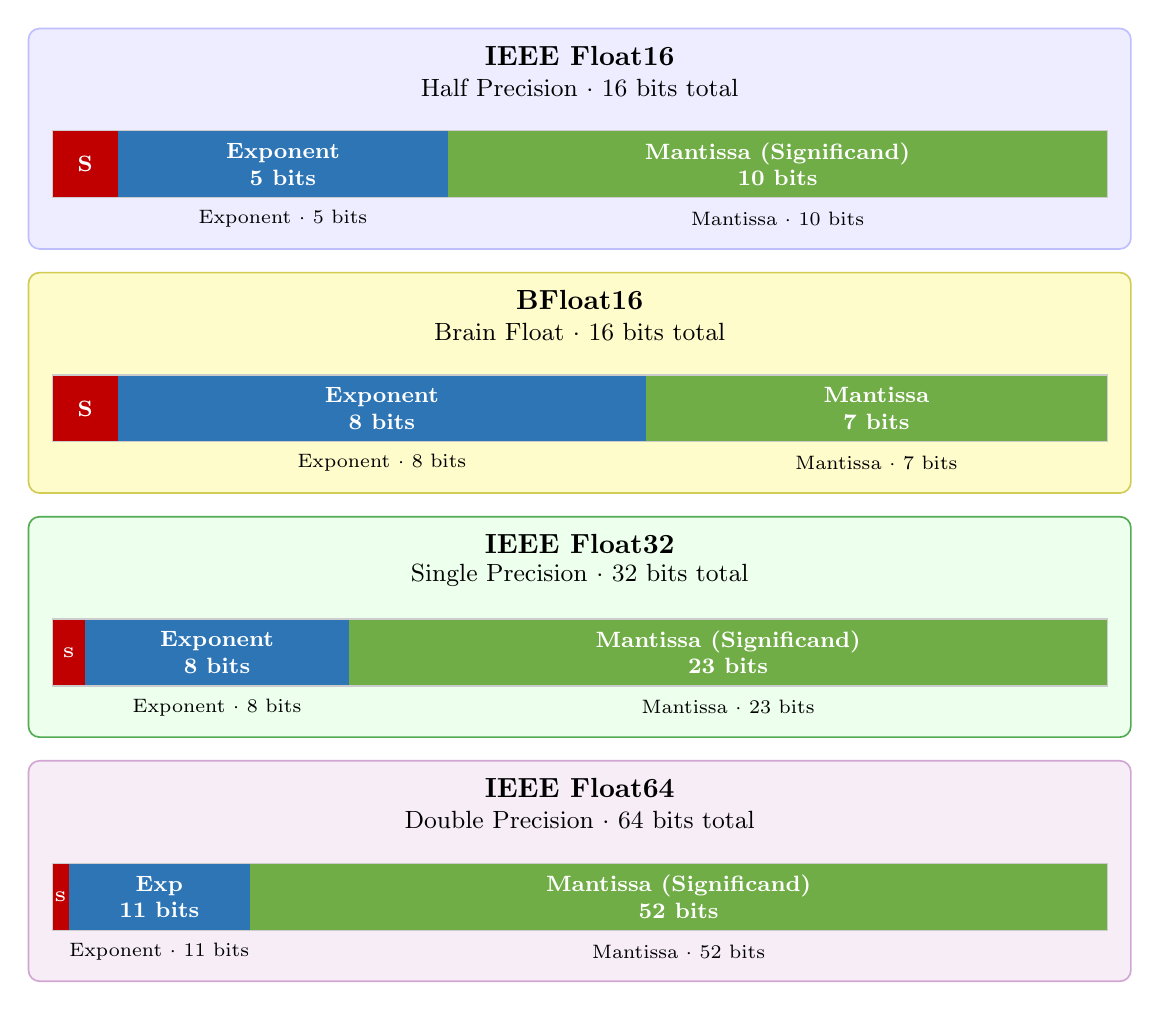
\begin{tikzpicture}[x=1cm, y=1cm]

  % ---- Color palette ----
  \definecolor{signcolor}{RGB}{192,0,0}     % red   -- sign bit
  \definecolor{expcolor} {RGB}{46,117,182}  % blue  -- exponent
  \definecolor{mancolor} {RGB}{112,173,71}  % green -- mantissa

  % ---- Panel backgrounds ----
  % Panels are 14 cm wide x 2.8 cm tall, separated by 0.3 cm gaps.
  % Y positions (bottom edge): Float16=9.30, BFloat16=6.20, Float32=3.10, Float64=0.00
  \draw[rounded corners=4pt, fill=blue!7,    draw=blue!25,        line width=0.6pt]
      (0.0,  9.30) rectangle (14.0, 12.10);  % Float16
  \draw[rounded corners=4pt, fill=yellow!20, draw=yellow!60!gray, line width=0.6pt]
      (0.0,  6.20) rectangle (14.0,  9.00);  % BFloat16
  \draw[rounded corners=4pt, fill=green!7,   draw=green!35!gray,  line width=0.6pt]
      (0.0,  3.10) rectangle (14.0,  5.90);  % Float32
  \draw[rounded corners=4pt, fill=violet!7,  draw=violet!35,      line width=0.6pt]
      (0.0,  0.00) rectangle (14.0,  2.80);  % Float64

  % ====================================================================
  % Bar geometry (shared across all panels):
  %   x range:    [0.30, 13.70]  => total bar width = 13.40 cm
  %   bar height: 0.85 cm
  %   bar bottom: panel_bottom + 0.65
  %   bar top:    panel_bottom + 1.50
  %
  % Segment x boundaries  (width = n_bits/total * 13.40):
  %   Float16  (16-bit): 0.300 | 1.138 | 5.325 | 13.700
  %   BFloat16 (16-bit): 0.300 | 1.138 | 7.838 | 13.700
  %   Float32  (32-bit): 0.300 | 0.719 | 4.069 | 13.700
  %   Float64  (64-bit): 0.300 | 0.509 | 2.813 | 13.700
  % ====================================================================

  % ------------------------------------------------------------------
  % IEEE Float16  (panel bottom y = 9.30)
  % ------------------------------------------------------------------
  \node[font=\normalsize\bfseries] at (7.0, 11.75) {IEEE Float16};
  \node[font=\small]               at (7.0, 11.35) {Half Precision $\cdot$ 16 bits total};

  % S:   1/16 * 13.40 = 0.838 cm   x: 0.300 -- 1.138,  center: 0.719
  \fill[signcolor] (0.300,  9.95) rectangle ( 1.138, 10.80);
  \node[text=white, font=\footnotesize\bfseries] at (0.719, 10.375) {S};

  % Exp: 5/16 * 13.40 = 4.188 cm   x: 1.138 -- 5.325,  center: 3.231
  \fill[expcolor]  (1.138,  9.95) rectangle ( 5.325, 10.80);
  \node[text=white, font=\footnotesize\bfseries, align=center] at (3.231, 10.375)
      {Exponent \\ 5 bits};

  % Man: 10/16 * 13.40 = 8.375 cm  x: 5.325 -- 13.700, center: 9.513
  \fill[mancolor]  (5.325,  9.95) rectangle (13.700, 10.80);
  \node[text=white, font=\footnotesize\bfseries, align=center] at (9.513, 10.375)
      {Mantissa (Significand) \\ 10 bits};

  \draw[black!20, line width=0.4pt] (0.300, 9.95) rectangle (13.700, 10.80);

  \node[font=\scriptsize] at (3.231, 9.68) {Exponent $\cdot$ 5 bits};
  \node[font=\scriptsize] at (9.513, 9.68) {Mantissa $\cdot$ 10 bits};

  % ------------------------------------------------------------------
  % BFloat16  (panel bottom y = 6.20)
  % ------------------------------------------------------------------
  \node[font=\normalsize\bfseries] at (7.0, 8.65) {BFloat16};
  \node[font=\small]               at (7.0, 8.25) {Brain Float $\cdot$ 16 bits total};

  % S:   1/16 * 13.40 = 0.838 cm   x: 0.300 -- 1.138,  center: 0.719
  \fill[signcolor] (0.300,  6.85) rectangle ( 1.138,  7.70);
  \node[text=white, font=\footnotesize\bfseries] at (0.719, 7.275) {S};

  % Exp: 8/16 * 13.40 = 6.700 cm   x: 1.138 -- 7.838,  center: 4.488
  \fill[expcolor]  (1.138,  6.85) rectangle ( 7.838,  7.70);
  \node[text=white, font=\footnotesize\bfseries, align=center] at (4.488, 7.275)
      {Exponent \\ 8 bits};

  % Man: 7/16 * 13.40 = 5.863 cm   x: 7.838 -- 13.700, center: 10.769
  \fill[mancolor]  (7.838,  6.85) rectangle (13.700,  7.70);
  \node[text=white, font=\footnotesize\bfseries, align=center] at (10.769, 7.275)
      {Mantissa \\ 7 bits};

  \draw[black!20, line width=0.4pt] (0.300, 6.85) rectangle (13.700, 7.70);

  \node[font=\scriptsize] at ( 4.488, 6.58) {Exponent $\cdot$ 8 bits};
  \node[font=\scriptsize] at (10.769, 6.58) {Mantissa $\cdot$ 7 bits};

  % ------------------------------------------------------------------
  % IEEE Float32  (panel bottom y = 3.10)
  % ------------------------------------------------------------------
  \node[font=\normalsize\bfseries] at (7.0, 5.55) {IEEE Float32};
  \node[font=\small]               at (7.0, 5.15) {Single Precision $\cdot$ 32 bits total};

  % S:   1/32 * 13.40 = 0.419 cm   x: 0.300 -- 0.719,  center: 0.510
  \fill[signcolor] (0.300,  3.75) rectangle ( 0.719,  4.60);
  \node[text=white, font=\tiny\bfseries] at (0.510, 4.175) {S};

  % Exp: 8/32 * 13.40 = 3.350 cm   x: 0.719 -- 4.069,  center: 2.394
  \fill[expcolor]  (0.719,  3.75) rectangle ( 4.069,  4.60);
  \node[text=white, font=\footnotesize\bfseries, align=center] at (2.394, 4.175)
      {Exponent \\ 8 bits};

  % Man: 23/32 * 13.40 = 9.631 cm  x: 4.069 -- 13.700, center: 8.885
  \fill[mancolor]  (4.069,  3.75) rectangle (13.700,  4.60);
  \node[text=white, font=\footnotesize\bfseries, align=center] at (8.885, 4.175)
      {Mantissa (Significand) \\ 23 bits};

  \draw[black!20, line width=0.4pt] (0.300, 3.75) rectangle (13.700, 4.60);

  \node[font=\scriptsize] at (2.394, 3.48) {Exponent $\cdot$ 8 bits};
  \node[font=\scriptsize] at (8.885, 3.48) {Mantissa $\cdot$ 23 bits};

  % ------------------------------------------------------------------
  % IEEE Float64  (panel bottom y = 0.00)
  % ------------------------------------------------------------------
  \node[font=\normalsize\bfseries] at (7.0, 2.45) {IEEE Float64};
  \node[font=\small]               at (7.0, 2.05) {Double Precision $\cdot$ 64 bits total};

  % S:    1/64 * 13.40 = 0.209 cm  x: 0.300 -- 0.509,  center: 0.405
  \fill[signcolor] (0.300,  0.65) rectangle ( 0.509,  1.50);
  \node[text=white, font=\tiny\bfseries] at (0.405, 1.075) {S};

  % Exp: 11/64 * 13.40 = 2.303 cm  x: 0.509 -- 2.813,  center: 1.661
  \fill[expcolor]  (0.509,  0.65) rectangle ( 2.813,  1.50);
  \node[text=white, font=\footnotesize\bfseries, align=center] at (1.661, 1.075)
      {Exp \\ 11 bits};

  % Man: 52/64 * 13.40 = 10.888 cm x: 2.813 -- 13.700, center: 8.257
  \fill[mancolor]  (2.813,  0.65) rectangle (13.700,  1.50);
  \node[text=white, font=\footnotesize\bfseries, align=center] at (8.257, 1.075)
      {Mantissa (Significand) \\ 52 bits};

  \draw[black!20, line width=0.4pt] (0.300, 0.65) rectangle (13.700, 1.50);

  \node[font=\scriptsize] at (1.661, 0.38) {Exponent $\cdot$ 11 bits};
  \node[font=\scriptsize] at (8.257, 0.38) {Mantissa $\cdot$ 52 bits};

\end{tikzpicture}
}
%
%   Fit to an arbitrary fraction of the column width:
%     \resizebox{0.9\columnwidth}{!}{% Floating-point format comparison — single-column stack layout
%
% Required in preamble:
%   \usepackage{tikz}
%
% ---- Scaling -------------------------------------------------------
% The tikzpicture is drawn at its natural size: 14 cm wide x 12.1 cm tall.
% Use \resizebox (from the graphicx package, always loaded in IEEE style)
% to scale it to whatever width you need. The height adjusts automatically.
%
%   Fit to a single text column (~8.8 cm in IEEE two-column):
%     \resizebox{\columnwidth}{!}{\input{float_formats_tikz.tex}}
%
%   Fit to the full page width (~17.8 cm in IEEE two-column):
%     \resizebox{\textwidth}{!}{\input{float_formats_tikz.tex}}
%
%   Fit to an arbitrary fraction of the column width:
%     \resizebox{0.9\columnwidth}{!}{\input{float_formats_tikz.tex}}
%
% \resizebox scales everything uniformly — coordinates, line widths,
% and fonts — so the result looks identical regardless of the chosen width.
%
% Recommended figure wrapper (single column):
%   \begin{figure}[t]
%     \centering
%     \resizebox{\columnwidth}{!}{\input{float_formats_tikz.tex}}
%     \caption{...}
%     \label{fig:float-formats}
%   \end{figure}
% --------------------------------------------------------------------
%
% Layout: 4 panels stacked vertically, each 14 cm x 2.8 cm.
% Bar widths are proportional to actual bit-field widths.
%   Float16:  S=1, Exp=5,  Man=10  (16 bits total)
%   BFloat16: S=1, Exp=8,  Man=7   (16 bits total)
%   Float32:  S=1, Exp=8,  Man=23  (32 bits total)
%   Float64:  S=1, Exp=11, Man=52  (64 bits total)

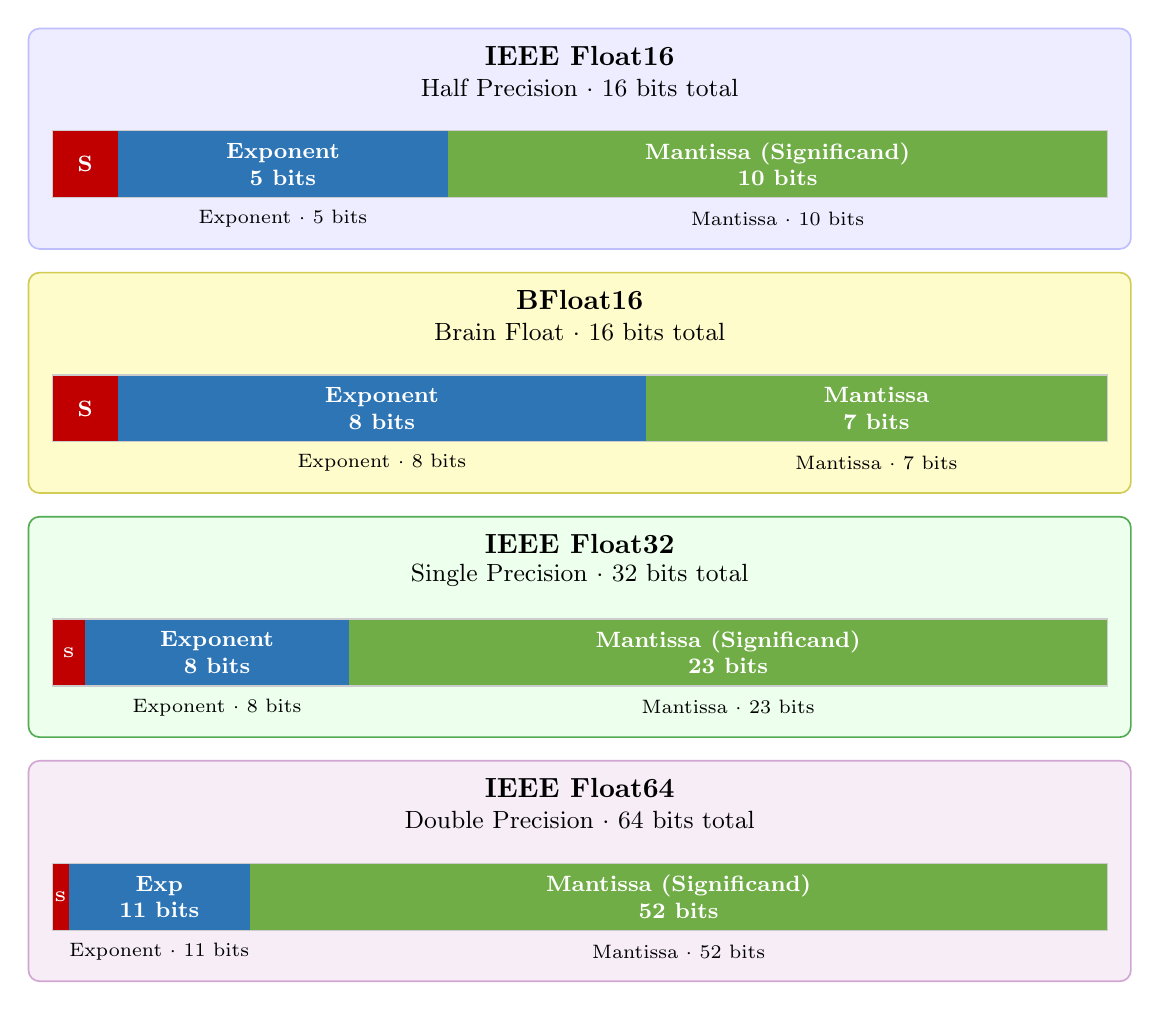
\begin{tikzpicture}[x=1cm, y=1cm]

  % ---- Color palette ----
  \definecolor{signcolor}{RGB}{192,0,0}     % red   -- sign bit
  \definecolor{expcolor} {RGB}{46,117,182}  % blue  -- exponent
  \definecolor{mancolor} {RGB}{112,173,71}  % green -- mantissa

  % ---- Panel backgrounds ----
  % Panels are 14 cm wide x 2.8 cm tall, separated by 0.3 cm gaps.
  % Y positions (bottom edge): Float16=9.30, BFloat16=6.20, Float32=3.10, Float64=0.00
  \draw[rounded corners=4pt, fill=blue!7,    draw=blue!25,        line width=0.6pt]
      (0.0,  9.30) rectangle (14.0, 12.10);  % Float16
  \draw[rounded corners=4pt, fill=yellow!20, draw=yellow!60!gray, line width=0.6pt]
      (0.0,  6.20) rectangle (14.0,  9.00);  % BFloat16
  \draw[rounded corners=4pt, fill=green!7,   draw=green!35!gray,  line width=0.6pt]
      (0.0,  3.10) rectangle (14.0,  5.90);  % Float32
  \draw[rounded corners=4pt, fill=violet!7,  draw=violet!35,      line width=0.6pt]
      (0.0,  0.00) rectangle (14.0,  2.80);  % Float64

  % ====================================================================
  % Bar geometry (shared across all panels):
  %   x range:    [0.30, 13.70]  => total bar width = 13.40 cm
  %   bar height: 0.85 cm
  %   bar bottom: panel_bottom + 0.65
  %   bar top:    panel_bottom + 1.50
  %
  % Segment x boundaries  (width = n_bits/total * 13.40):
  %   Float16  (16-bit): 0.300 | 1.138 | 5.325 | 13.700
  %   BFloat16 (16-bit): 0.300 | 1.138 | 7.838 | 13.700
  %   Float32  (32-bit): 0.300 | 0.719 | 4.069 | 13.700
  %   Float64  (64-bit): 0.300 | 0.509 | 2.813 | 13.700
  % ====================================================================

  % ------------------------------------------------------------------
  % IEEE Float16  (panel bottom y = 9.30)
  % ------------------------------------------------------------------
  \node[font=\normalsize\bfseries] at (7.0, 11.75) {IEEE Float16};
  \node[font=\small]               at (7.0, 11.35) {Half Precision $\cdot$ 16 bits total};

  % S:   1/16 * 13.40 = 0.838 cm   x: 0.300 -- 1.138,  center: 0.719
  \fill[signcolor] (0.300,  9.95) rectangle ( 1.138, 10.80);
  \node[text=white, font=\footnotesize\bfseries] at (0.719, 10.375) {S};

  % Exp: 5/16 * 13.40 = 4.188 cm   x: 1.138 -- 5.325,  center: 3.231
  \fill[expcolor]  (1.138,  9.95) rectangle ( 5.325, 10.80);
  \node[text=white, font=\footnotesize\bfseries, align=center] at (3.231, 10.375)
      {Exponent \\ 5 bits};

  % Man: 10/16 * 13.40 = 8.375 cm  x: 5.325 -- 13.700, center: 9.513
  \fill[mancolor]  (5.325,  9.95) rectangle (13.700, 10.80);
  \node[text=white, font=\footnotesize\bfseries, align=center] at (9.513, 10.375)
      {Mantissa (Significand) \\ 10 bits};

  \draw[black!20, line width=0.4pt] (0.300, 9.95) rectangle (13.700, 10.80);

  \node[font=\scriptsize] at (3.231, 9.68) {Exponent $\cdot$ 5 bits};
  \node[font=\scriptsize] at (9.513, 9.68) {Mantissa $\cdot$ 10 bits};

  % ------------------------------------------------------------------
  % BFloat16  (panel bottom y = 6.20)
  % ------------------------------------------------------------------
  \node[font=\normalsize\bfseries] at (7.0, 8.65) {BFloat16};
  \node[font=\small]               at (7.0, 8.25) {Brain Float $\cdot$ 16 bits total};

  % S:   1/16 * 13.40 = 0.838 cm   x: 0.300 -- 1.138,  center: 0.719
  \fill[signcolor] (0.300,  6.85) rectangle ( 1.138,  7.70);
  \node[text=white, font=\footnotesize\bfseries] at (0.719, 7.275) {S};

  % Exp: 8/16 * 13.40 = 6.700 cm   x: 1.138 -- 7.838,  center: 4.488
  \fill[expcolor]  (1.138,  6.85) rectangle ( 7.838,  7.70);
  \node[text=white, font=\footnotesize\bfseries, align=center] at (4.488, 7.275)
      {Exponent \\ 8 bits};

  % Man: 7/16 * 13.40 = 5.863 cm   x: 7.838 -- 13.700, center: 10.769
  \fill[mancolor]  (7.838,  6.85) rectangle (13.700,  7.70);
  \node[text=white, font=\footnotesize\bfseries, align=center] at (10.769, 7.275)
      {Mantissa \\ 7 bits};

  \draw[black!20, line width=0.4pt] (0.300, 6.85) rectangle (13.700, 7.70);

  \node[font=\scriptsize] at ( 4.488, 6.58) {Exponent $\cdot$ 8 bits};
  \node[font=\scriptsize] at (10.769, 6.58) {Mantissa $\cdot$ 7 bits};

  % ------------------------------------------------------------------
  % IEEE Float32  (panel bottom y = 3.10)
  % ------------------------------------------------------------------
  \node[font=\normalsize\bfseries] at (7.0, 5.55) {IEEE Float32};
  \node[font=\small]               at (7.0, 5.15) {Single Precision $\cdot$ 32 bits total};

  % S:   1/32 * 13.40 = 0.419 cm   x: 0.300 -- 0.719,  center: 0.510
  \fill[signcolor] (0.300,  3.75) rectangle ( 0.719,  4.60);
  \node[text=white, font=\tiny\bfseries] at (0.510, 4.175) {S};

  % Exp: 8/32 * 13.40 = 3.350 cm   x: 0.719 -- 4.069,  center: 2.394
  \fill[expcolor]  (0.719,  3.75) rectangle ( 4.069,  4.60);
  \node[text=white, font=\footnotesize\bfseries, align=center] at (2.394, 4.175)
      {Exponent \\ 8 bits};

  % Man: 23/32 * 13.40 = 9.631 cm  x: 4.069 -- 13.700, center: 8.885
  \fill[mancolor]  (4.069,  3.75) rectangle (13.700,  4.60);
  \node[text=white, font=\footnotesize\bfseries, align=center] at (8.885, 4.175)
      {Mantissa (Significand) \\ 23 bits};

  \draw[black!20, line width=0.4pt] (0.300, 3.75) rectangle (13.700, 4.60);

  \node[font=\scriptsize] at (2.394, 3.48) {Exponent $\cdot$ 8 bits};
  \node[font=\scriptsize] at (8.885, 3.48) {Mantissa $\cdot$ 23 bits};

  % ------------------------------------------------------------------
  % IEEE Float64  (panel bottom y = 0.00)
  % ------------------------------------------------------------------
  \node[font=\normalsize\bfseries] at (7.0, 2.45) {IEEE Float64};
  \node[font=\small]               at (7.0, 2.05) {Double Precision $\cdot$ 64 bits total};

  % S:    1/64 * 13.40 = 0.209 cm  x: 0.300 -- 0.509,  center: 0.405
  \fill[signcolor] (0.300,  0.65) rectangle ( 0.509,  1.50);
  \node[text=white, font=\tiny\bfseries] at (0.405, 1.075) {S};

  % Exp: 11/64 * 13.40 = 2.303 cm  x: 0.509 -- 2.813,  center: 1.661
  \fill[expcolor]  (0.509,  0.65) rectangle ( 2.813,  1.50);
  \node[text=white, font=\footnotesize\bfseries, align=center] at (1.661, 1.075)
      {Exp \\ 11 bits};

  % Man: 52/64 * 13.40 = 10.888 cm x: 2.813 -- 13.700, center: 8.257
  \fill[mancolor]  (2.813,  0.65) rectangle (13.700,  1.50);
  \node[text=white, font=\footnotesize\bfseries, align=center] at (8.257, 1.075)
      {Mantissa (Significand) \\ 52 bits};

  \draw[black!20, line width=0.4pt] (0.300, 0.65) rectangle (13.700, 1.50);

  \node[font=\scriptsize] at (1.661, 0.38) {Exponent $\cdot$ 11 bits};
  \node[font=\scriptsize] at (8.257, 0.38) {Mantissa $\cdot$ 52 bits};

\end{tikzpicture}
}
%
% \resizebox scales everything uniformly — coordinates, line widths,
% and fonts — so the result looks identical regardless of the chosen width.
%
% Recommended figure wrapper (single column):
%   \begin{figure}[t]
%     \centering
%     \resizebox{\columnwidth}{!}{% Floating-point format comparison — single-column stack layout
%
% Required in preamble:
%   \usepackage{tikz}
%
% ---- Scaling -------------------------------------------------------
% The tikzpicture is drawn at its natural size: 14 cm wide x 12.1 cm tall.
% Use \resizebox (from the graphicx package, always loaded in IEEE style)
% to scale it to whatever width you need. The height adjusts automatically.
%
%   Fit to a single text column (~8.8 cm in IEEE two-column):
%     \resizebox{\columnwidth}{!}{\input{float_formats_tikz.tex}}
%
%   Fit to the full page width (~17.8 cm in IEEE two-column):
%     \resizebox{\textwidth}{!}{\input{float_formats_tikz.tex}}
%
%   Fit to an arbitrary fraction of the column width:
%     \resizebox{0.9\columnwidth}{!}{\input{float_formats_tikz.tex}}
%
% \resizebox scales everything uniformly — coordinates, line widths,
% and fonts — so the result looks identical regardless of the chosen width.
%
% Recommended figure wrapper (single column):
%   \begin{figure}[t]
%     \centering
%     \resizebox{\columnwidth}{!}{\input{float_formats_tikz.tex}}
%     \caption{...}
%     \label{fig:float-formats}
%   \end{figure}
% --------------------------------------------------------------------
%
% Layout: 4 panels stacked vertically, each 14 cm x 2.8 cm.
% Bar widths are proportional to actual bit-field widths.
%   Float16:  S=1, Exp=5,  Man=10  (16 bits total)
%   BFloat16: S=1, Exp=8,  Man=7   (16 bits total)
%   Float32:  S=1, Exp=8,  Man=23  (32 bits total)
%   Float64:  S=1, Exp=11, Man=52  (64 bits total)

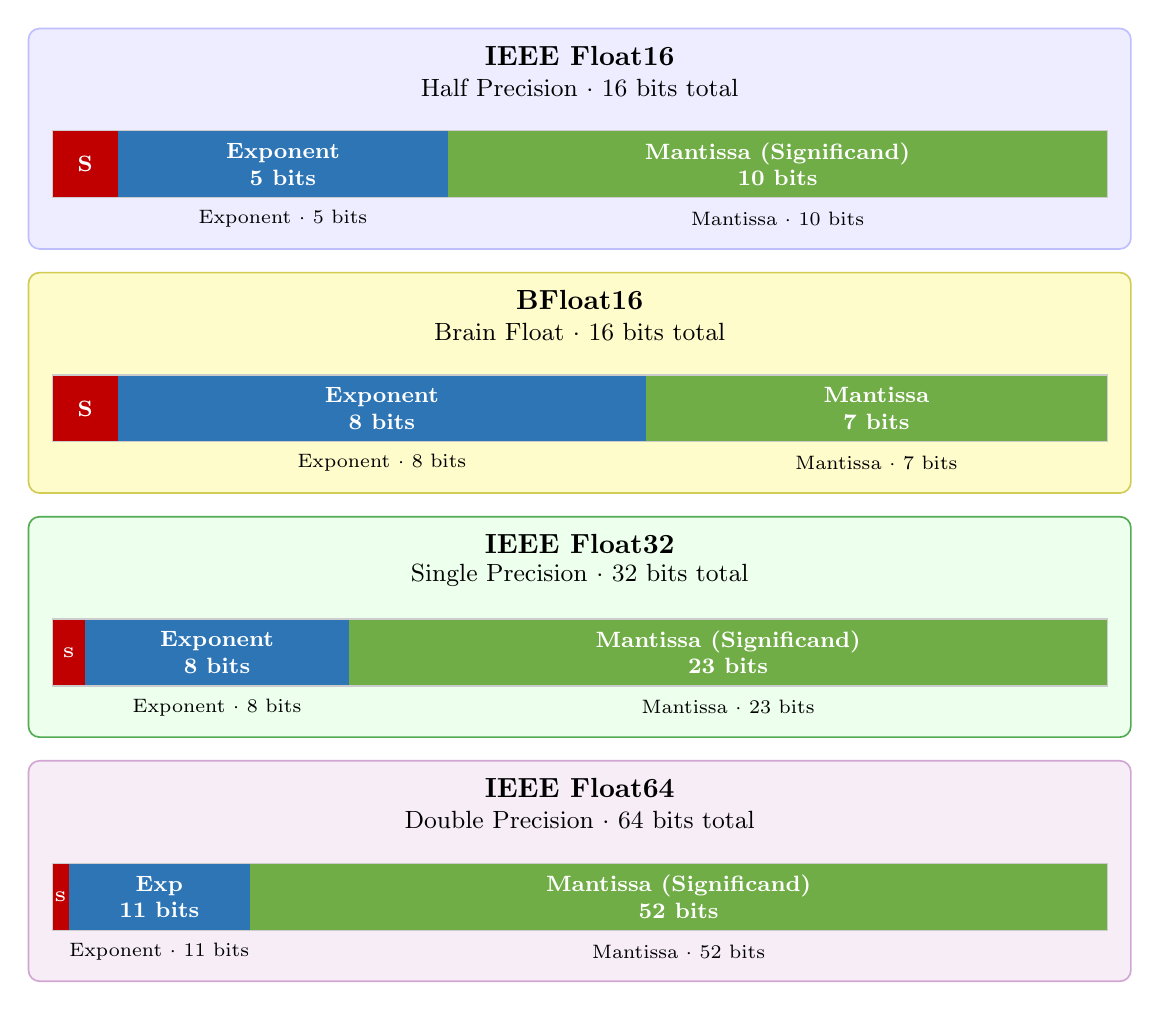
\begin{tikzpicture}[x=1cm, y=1cm]

  % ---- Color palette ----
  \definecolor{signcolor}{RGB}{192,0,0}     % red   -- sign bit
  \definecolor{expcolor} {RGB}{46,117,182}  % blue  -- exponent
  \definecolor{mancolor} {RGB}{112,173,71}  % green -- mantissa

  % ---- Panel backgrounds ----
  % Panels are 14 cm wide x 2.8 cm tall, separated by 0.3 cm gaps.
  % Y positions (bottom edge): Float16=9.30, BFloat16=6.20, Float32=3.10, Float64=0.00
  \draw[rounded corners=4pt, fill=blue!7,    draw=blue!25,        line width=0.6pt]
      (0.0,  9.30) rectangle (14.0, 12.10);  % Float16
  \draw[rounded corners=4pt, fill=yellow!20, draw=yellow!60!gray, line width=0.6pt]
      (0.0,  6.20) rectangle (14.0,  9.00);  % BFloat16
  \draw[rounded corners=4pt, fill=green!7,   draw=green!35!gray,  line width=0.6pt]
      (0.0,  3.10) rectangle (14.0,  5.90);  % Float32
  \draw[rounded corners=4pt, fill=violet!7,  draw=violet!35,      line width=0.6pt]
      (0.0,  0.00) rectangle (14.0,  2.80);  % Float64

  % ====================================================================
  % Bar geometry (shared across all panels):
  %   x range:    [0.30, 13.70]  => total bar width = 13.40 cm
  %   bar height: 0.85 cm
  %   bar bottom: panel_bottom + 0.65
  %   bar top:    panel_bottom + 1.50
  %
  % Segment x boundaries  (width = n_bits/total * 13.40):
  %   Float16  (16-bit): 0.300 | 1.138 | 5.325 | 13.700
  %   BFloat16 (16-bit): 0.300 | 1.138 | 7.838 | 13.700
  %   Float32  (32-bit): 0.300 | 0.719 | 4.069 | 13.700
  %   Float64  (64-bit): 0.300 | 0.509 | 2.813 | 13.700
  % ====================================================================

  % ------------------------------------------------------------------
  % IEEE Float16  (panel bottom y = 9.30)
  % ------------------------------------------------------------------
  \node[font=\normalsize\bfseries] at (7.0, 11.75) {IEEE Float16};
  \node[font=\small]               at (7.0, 11.35) {Half Precision $\cdot$ 16 bits total};

  % S:   1/16 * 13.40 = 0.838 cm   x: 0.300 -- 1.138,  center: 0.719
  \fill[signcolor] (0.300,  9.95) rectangle ( 1.138, 10.80);
  \node[text=white, font=\footnotesize\bfseries] at (0.719, 10.375) {S};

  % Exp: 5/16 * 13.40 = 4.188 cm   x: 1.138 -- 5.325,  center: 3.231
  \fill[expcolor]  (1.138,  9.95) rectangle ( 5.325, 10.80);
  \node[text=white, font=\footnotesize\bfseries, align=center] at (3.231, 10.375)
      {Exponent \\ 5 bits};

  % Man: 10/16 * 13.40 = 8.375 cm  x: 5.325 -- 13.700, center: 9.513
  \fill[mancolor]  (5.325,  9.95) rectangle (13.700, 10.80);
  \node[text=white, font=\footnotesize\bfseries, align=center] at (9.513, 10.375)
      {Mantissa (Significand) \\ 10 bits};

  \draw[black!20, line width=0.4pt] (0.300, 9.95) rectangle (13.700, 10.80);

  \node[font=\scriptsize] at (3.231, 9.68) {Exponent $\cdot$ 5 bits};
  \node[font=\scriptsize] at (9.513, 9.68) {Mantissa $\cdot$ 10 bits};

  % ------------------------------------------------------------------
  % BFloat16  (panel bottom y = 6.20)
  % ------------------------------------------------------------------
  \node[font=\normalsize\bfseries] at (7.0, 8.65) {BFloat16};
  \node[font=\small]               at (7.0, 8.25) {Brain Float $\cdot$ 16 bits total};

  % S:   1/16 * 13.40 = 0.838 cm   x: 0.300 -- 1.138,  center: 0.719
  \fill[signcolor] (0.300,  6.85) rectangle ( 1.138,  7.70);
  \node[text=white, font=\footnotesize\bfseries] at (0.719, 7.275) {S};

  % Exp: 8/16 * 13.40 = 6.700 cm   x: 1.138 -- 7.838,  center: 4.488
  \fill[expcolor]  (1.138,  6.85) rectangle ( 7.838,  7.70);
  \node[text=white, font=\footnotesize\bfseries, align=center] at (4.488, 7.275)
      {Exponent \\ 8 bits};

  % Man: 7/16 * 13.40 = 5.863 cm   x: 7.838 -- 13.700, center: 10.769
  \fill[mancolor]  (7.838,  6.85) rectangle (13.700,  7.70);
  \node[text=white, font=\footnotesize\bfseries, align=center] at (10.769, 7.275)
      {Mantissa \\ 7 bits};

  \draw[black!20, line width=0.4pt] (0.300, 6.85) rectangle (13.700, 7.70);

  \node[font=\scriptsize] at ( 4.488, 6.58) {Exponent $\cdot$ 8 bits};
  \node[font=\scriptsize] at (10.769, 6.58) {Mantissa $\cdot$ 7 bits};

  % ------------------------------------------------------------------
  % IEEE Float32  (panel bottom y = 3.10)
  % ------------------------------------------------------------------
  \node[font=\normalsize\bfseries] at (7.0, 5.55) {IEEE Float32};
  \node[font=\small]               at (7.0, 5.15) {Single Precision $\cdot$ 32 bits total};

  % S:   1/32 * 13.40 = 0.419 cm   x: 0.300 -- 0.719,  center: 0.510
  \fill[signcolor] (0.300,  3.75) rectangle ( 0.719,  4.60);
  \node[text=white, font=\tiny\bfseries] at (0.510, 4.175) {S};

  % Exp: 8/32 * 13.40 = 3.350 cm   x: 0.719 -- 4.069,  center: 2.394
  \fill[expcolor]  (0.719,  3.75) rectangle ( 4.069,  4.60);
  \node[text=white, font=\footnotesize\bfseries, align=center] at (2.394, 4.175)
      {Exponent \\ 8 bits};

  % Man: 23/32 * 13.40 = 9.631 cm  x: 4.069 -- 13.700, center: 8.885
  \fill[mancolor]  (4.069,  3.75) rectangle (13.700,  4.60);
  \node[text=white, font=\footnotesize\bfseries, align=center] at (8.885, 4.175)
      {Mantissa (Significand) \\ 23 bits};

  \draw[black!20, line width=0.4pt] (0.300, 3.75) rectangle (13.700, 4.60);

  \node[font=\scriptsize] at (2.394, 3.48) {Exponent $\cdot$ 8 bits};
  \node[font=\scriptsize] at (8.885, 3.48) {Mantissa $\cdot$ 23 bits};

  % ------------------------------------------------------------------
  % IEEE Float64  (panel bottom y = 0.00)
  % ------------------------------------------------------------------
  \node[font=\normalsize\bfseries] at (7.0, 2.45) {IEEE Float64};
  \node[font=\small]               at (7.0, 2.05) {Double Precision $\cdot$ 64 bits total};

  % S:    1/64 * 13.40 = 0.209 cm  x: 0.300 -- 0.509,  center: 0.405
  \fill[signcolor] (0.300,  0.65) rectangle ( 0.509,  1.50);
  \node[text=white, font=\tiny\bfseries] at (0.405, 1.075) {S};

  % Exp: 11/64 * 13.40 = 2.303 cm  x: 0.509 -- 2.813,  center: 1.661
  \fill[expcolor]  (0.509,  0.65) rectangle ( 2.813,  1.50);
  \node[text=white, font=\footnotesize\bfseries, align=center] at (1.661, 1.075)
      {Exp \\ 11 bits};

  % Man: 52/64 * 13.40 = 10.888 cm x: 2.813 -- 13.700, center: 8.257
  \fill[mancolor]  (2.813,  0.65) rectangle (13.700,  1.50);
  \node[text=white, font=\footnotesize\bfseries, align=center] at (8.257, 1.075)
      {Mantissa (Significand) \\ 52 bits};

  \draw[black!20, line width=0.4pt] (0.300, 0.65) rectangle (13.700, 1.50);

  \node[font=\scriptsize] at (1.661, 0.38) {Exponent $\cdot$ 11 bits};
  \node[font=\scriptsize] at (8.257, 0.38) {Mantissa $\cdot$ 52 bits};

\end{tikzpicture}
}
%     \caption{...}
%     \label{fig:float-formats}
%   \end{figure}
% --------------------------------------------------------------------
%
% Layout: 4 panels stacked vertically, each 14 cm x 2.8 cm.
% Bar widths are proportional to actual bit-field widths.
%   Float16:  S=1, Exp=5,  Man=10  (16 bits total)
%   BFloat16: S=1, Exp=8,  Man=7   (16 bits total)
%   Float32:  S=1, Exp=8,  Man=23  (32 bits total)
%   Float64:  S=1, Exp=11, Man=52  (64 bits total)

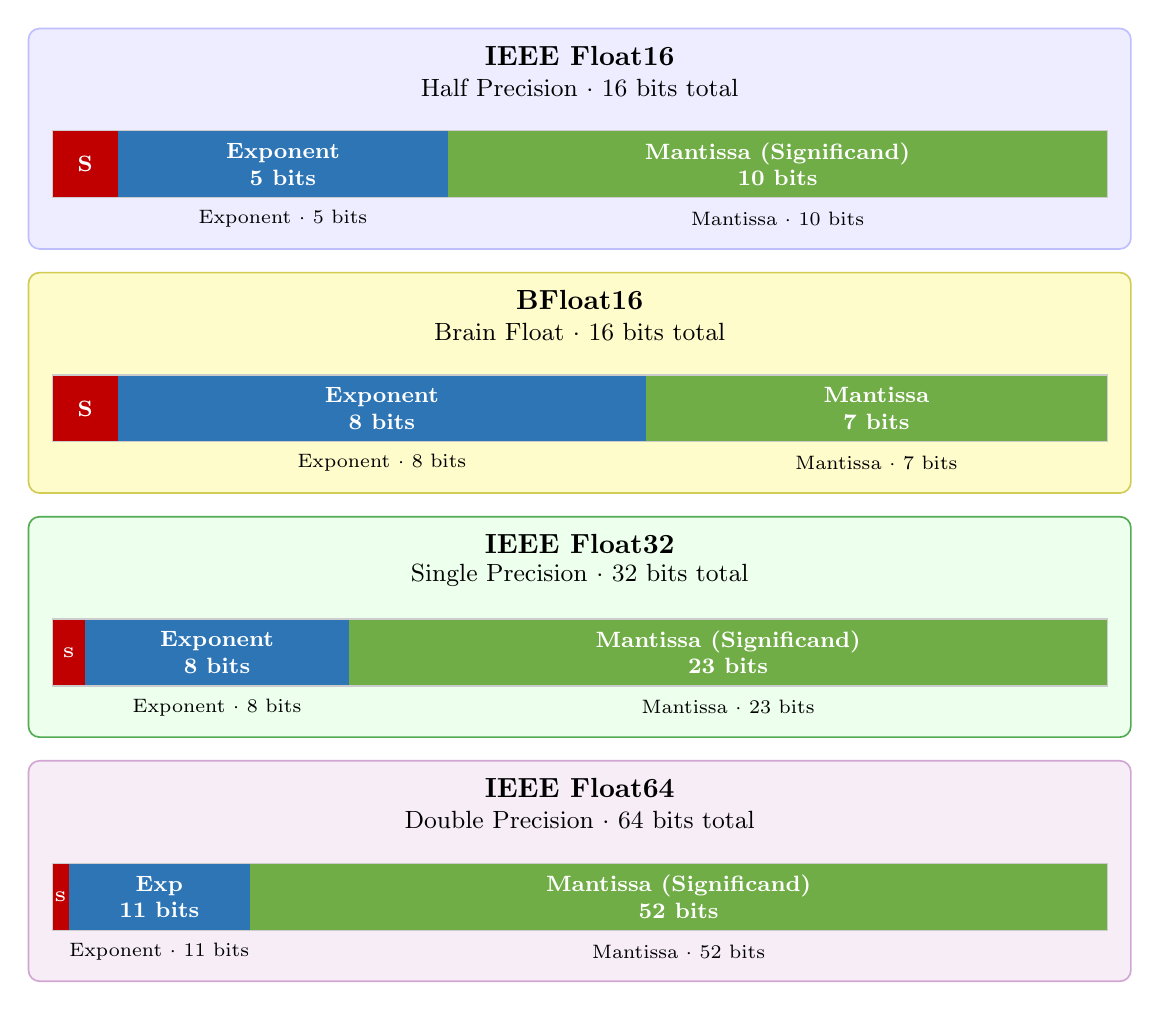
\begin{tikzpicture}[x=1cm, y=1cm]

  % ---- Color palette ----
  \definecolor{signcolor}{RGB}{192,0,0}     % red   -- sign bit
  \definecolor{expcolor} {RGB}{46,117,182}  % blue  -- exponent
  \definecolor{mancolor} {RGB}{112,173,71}  % green -- mantissa

  % ---- Panel backgrounds ----
  % Panels are 14 cm wide x 2.8 cm tall, separated by 0.3 cm gaps.
  % Y positions (bottom edge): Float16=9.30, BFloat16=6.20, Float32=3.10, Float64=0.00
  \draw[rounded corners=4pt, fill=blue!7,    draw=blue!25,        line width=0.6pt]
      (0.0,  9.30) rectangle (14.0, 12.10);  % Float16
  \draw[rounded corners=4pt, fill=yellow!20, draw=yellow!60!gray, line width=0.6pt]
      (0.0,  6.20) rectangle (14.0,  9.00);  % BFloat16
  \draw[rounded corners=4pt, fill=green!7,   draw=green!35!gray,  line width=0.6pt]
      (0.0,  3.10) rectangle (14.0,  5.90);  % Float32
  \draw[rounded corners=4pt, fill=violet!7,  draw=violet!35,      line width=0.6pt]
      (0.0,  0.00) rectangle (14.0,  2.80);  % Float64

  % ====================================================================
  % Bar geometry (shared across all panels):
  %   x range:    [0.30, 13.70]  => total bar width = 13.40 cm
  %   bar height: 0.85 cm
  %   bar bottom: panel_bottom + 0.65
  %   bar top:    panel_bottom + 1.50
  %
  % Segment x boundaries  (width = n_bits/total * 13.40):
  %   Float16  (16-bit): 0.300 | 1.138 | 5.325 | 13.700
  %   BFloat16 (16-bit): 0.300 | 1.138 | 7.838 | 13.700
  %   Float32  (32-bit): 0.300 | 0.719 | 4.069 | 13.700
  %   Float64  (64-bit): 0.300 | 0.509 | 2.813 | 13.700
  % ====================================================================

  % ------------------------------------------------------------------
  % IEEE Float16  (panel bottom y = 9.30)
  % ------------------------------------------------------------------
  \node[font=\normalsize\bfseries] at (7.0, 11.75) {IEEE Float16};
  \node[font=\small]               at (7.0, 11.35) {Half Precision $\cdot$ 16 bits total};

  % S:   1/16 * 13.40 = 0.838 cm   x: 0.300 -- 1.138,  center: 0.719
  \fill[signcolor] (0.300,  9.95) rectangle ( 1.138, 10.80);
  \node[text=white, font=\footnotesize\bfseries] at (0.719, 10.375) {S};

  % Exp: 5/16 * 13.40 = 4.188 cm   x: 1.138 -- 5.325,  center: 3.231
  \fill[expcolor]  (1.138,  9.95) rectangle ( 5.325, 10.80);
  \node[text=white, font=\footnotesize\bfseries, align=center] at (3.231, 10.375)
      {Exponent \\ 5 bits};

  % Man: 10/16 * 13.40 = 8.375 cm  x: 5.325 -- 13.700, center: 9.513
  \fill[mancolor]  (5.325,  9.95) rectangle (13.700, 10.80);
  \node[text=white, font=\footnotesize\bfseries, align=center] at (9.513, 10.375)
      {Mantissa (Significand) \\ 10 bits};

  \draw[black!20, line width=0.4pt] (0.300, 9.95) rectangle (13.700, 10.80);

  \node[font=\scriptsize] at (3.231, 9.68) {Exponent $\cdot$ 5 bits};
  \node[font=\scriptsize] at (9.513, 9.68) {Mantissa $\cdot$ 10 bits};

  % ------------------------------------------------------------------
  % BFloat16  (panel bottom y = 6.20)
  % ------------------------------------------------------------------
  \node[font=\normalsize\bfseries] at (7.0, 8.65) {BFloat16};
  \node[font=\small]               at (7.0, 8.25) {Brain Float $\cdot$ 16 bits total};

  % S:   1/16 * 13.40 = 0.838 cm   x: 0.300 -- 1.138,  center: 0.719
  \fill[signcolor] (0.300,  6.85) rectangle ( 1.138,  7.70);
  \node[text=white, font=\footnotesize\bfseries] at (0.719, 7.275) {S};

  % Exp: 8/16 * 13.40 = 6.700 cm   x: 1.138 -- 7.838,  center: 4.488
  \fill[expcolor]  (1.138,  6.85) rectangle ( 7.838,  7.70);
  \node[text=white, font=\footnotesize\bfseries, align=center] at (4.488, 7.275)
      {Exponent \\ 8 bits};

  % Man: 7/16 * 13.40 = 5.863 cm   x: 7.838 -- 13.700, center: 10.769
  \fill[mancolor]  (7.838,  6.85) rectangle (13.700,  7.70);
  \node[text=white, font=\footnotesize\bfseries, align=center] at (10.769, 7.275)
      {Mantissa \\ 7 bits};

  \draw[black!20, line width=0.4pt] (0.300, 6.85) rectangle (13.700, 7.70);

  \node[font=\scriptsize] at ( 4.488, 6.58) {Exponent $\cdot$ 8 bits};
  \node[font=\scriptsize] at (10.769, 6.58) {Mantissa $\cdot$ 7 bits};

  % ------------------------------------------------------------------
  % IEEE Float32  (panel bottom y = 3.10)
  % ------------------------------------------------------------------
  \node[font=\normalsize\bfseries] at (7.0, 5.55) {IEEE Float32};
  \node[font=\small]               at (7.0, 5.15) {Single Precision $\cdot$ 32 bits total};

  % S:   1/32 * 13.40 = 0.419 cm   x: 0.300 -- 0.719,  center: 0.510
  \fill[signcolor] (0.300,  3.75) rectangle ( 0.719,  4.60);
  \node[text=white, font=\tiny\bfseries] at (0.510, 4.175) {S};

  % Exp: 8/32 * 13.40 = 3.350 cm   x: 0.719 -- 4.069,  center: 2.394
  \fill[expcolor]  (0.719,  3.75) rectangle ( 4.069,  4.60);
  \node[text=white, font=\footnotesize\bfseries, align=center] at (2.394, 4.175)
      {Exponent \\ 8 bits};

  % Man: 23/32 * 13.40 = 9.631 cm  x: 4.069 -- 13.700, center: 8.885
  \fill[mancolor]  (4.069,  3.75) rectangle (13.700,  4.60);
  \node[text=white, font=\footnotesize\bfseries, align=center] at (8.885, 4.175)
      {Mantissa (Significand) \\ 23 bits};

  \draw[black!20, line width=0.4pt] (0.300, 3.75) rectangle (13.700, 4.60);

  \node[font=\scriptsize] at (2.394, 3.48) {Exponent $\cdot$ 8 bits};
  \node[font=\scriptsize] at (8.885, 3.48) {Mantissa $\cdot$ 23 bits};

  % ------------------------------------------------------------------
  % IEEE Float64  (panel bottom y = 0.00)
  % ------------------------------------------------------------------
  \node[font=\normalsize\bfseries] at (7.0, 2.45) {IEEE Float64};
  \node[font=\small]               at (7.0, 2.05) {Double Precision $\cdot$ 64 bits total};

  % S:    1/64 * 13.40 = 0.209 cm  x: 0.300 -- 0.509,  center: 0.405
  \fill[signcolor] (0.300,  0.65) rectangle ( 0.509,  1.50);
  \node[text=white, font=\tiny\bfseries] at (0.405, 1.075) {S};

  % Exp: 11/64 * 13.40 = 2.303 cm  x: 0.509 -- 2.813,  center: 1.661
  \fill[expcolor]  (0.509,  0.65) rectangle ( 2.813,  1.50);
  \node[text=white, font=\footnotesize\bfseries, align=center] at (1.661, 1.075)
      {Exp \\ 11 bits};

  % Man: 52/64 * 13.40 = 10.888 cm x: 2.813 -- 13.700, center: 8.257
  \fill[mancolor]  (2.813,  0.65) rectangle (13.700,  1.50);
  \node[text=white, font=\footnotesize\bfseries, align=center] at (8.257, 1.075)
      {Mantissa (Significand) \\ 52 bits};

  \draw[black!20, line width=0.4pt] (0.300, 0.65) rectangle (13.700, 1.50);

  \node[font=\scriptsize] at (1.661, 0.38) {Exponent $\cdot$ 11 bits};
  \node[font=\scriptsize] at (8.257, 0.38) {Mantissa $\cdot$ 52 bits};

\end{tikzpicture}
}
%
% \resizebox scales everything uniformly — coordinates, line widths,
% and fonts — so the result looks identical regardless of the chosen width.
%
% Recommended figure wrapper (single column):
%   \begin{figure}[t]
%     \centering
%     \resizebox{\columnwidth}{!}{% Floating-point format comparison — single-column stack layout
%
% Required in preamble:
%   \usepackage{tikz}
%
% ---- Scaling -------------------------------------------------------
% The tikzpicture is drawn at its natural size: 14 cm wide x 12.1 cm tall.
% Use \resizebox (from the graphicx package, always loaded in IEEE style)
% to scale it to whatever width you need. The height adjusts automatically.
%
%   Fit to a single text column (~8.8 cm in IEEE two-column):
%     \resizebox{\columnwidth}{!}{% Floating-point format comparison — single-column stack layout
%
% Required in preamble:
%   \usepackage{tikz}
%
% ---- Scaling -------------------------------------------------------
% The tikzpicture is drawn at its natural size: 14 cm wide x 12.1 cm tall.
% Use \resizebox (from the graphicx package, always loaded in IEEE style)
% to scale it to whatever width you need. The height adjusts automatically.
%
%   Fit to a single text column (~8.8 cm in IEEE two-column):
%     \resizebox{\columnwidth}{!}{\input{float_formats_tikz.tex}}
%
%   Fit to the full page width (~17.8 cm in IEEE two-column):
%     \resizebox{\textwidth}{!}{\input{float_formats_tikz.tex}}
%
%   Fit to an arbitrary fraction of the column width:
%     \resizebox{0.9\columnwidth}{!}{\input{float_formats_tikz.tex}}
%
% \resizebox scales everything uniformly — coordinates, line widths,
% and fonts — so the result looks identical regardless of the chosen width.
%
% Recommended figure wrapper (single column):
%   \begin{figure}[t]
%     \centering
%     \resizebox{\columnwidth}{!}{\input{float_formats_tikz.tex}}
%     \caption{...}
%     \label{fig:float-formats}
%   \end{figure}
% --------------------------------------------------------------------
%
% Layout: 4 panels stacked vertically, each 14 cm x 2.8 cm.
% Bar widths are proportional to actual bit-field widths.
%   Float16:  S=1, Exp=5,  Man=10  (16 bits total)
%   BFloat16: S=1, Exp=8,  Man=7   (16 bits total)
%   Float32:  S=1, Exp=8,  Man=23  (32 bits total)
%   Float64:  S=1, Exp=11, Man=52  (64 bits total)

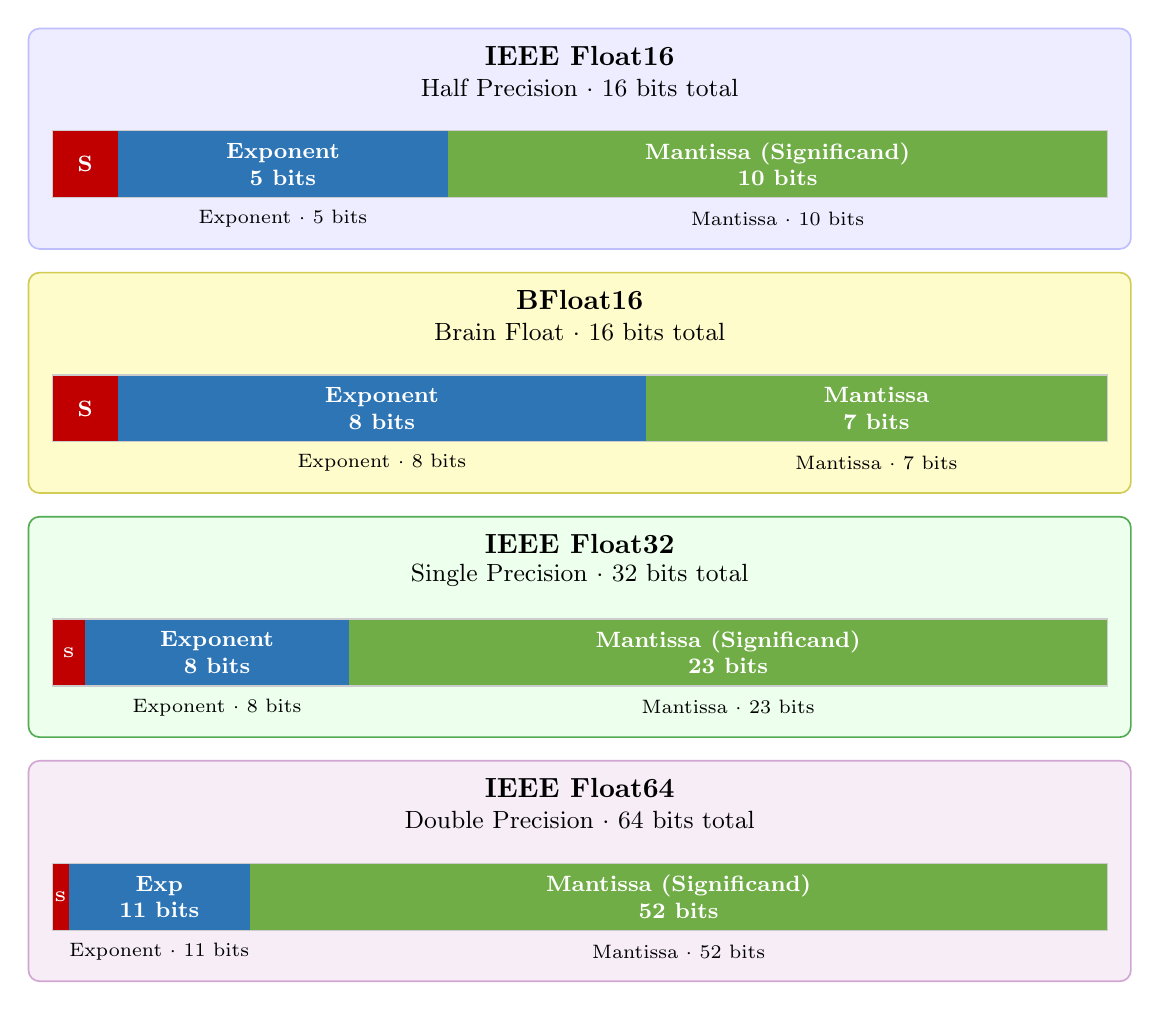
\begin{tikzpicture}[x=1cm, y=1cm]

  % ---- Color palette ----
  \definecolor{signcolor}{RGB}{192,0,0}     % red   -- sign bit
  \definecolor{expcolor} {RGB}{46,117,182}  % blue  -- exponent
  \definecolor{mancolor} {RGB}{112,173,71}  % green -- mantissa

  % ---- Panel backgrounds ----
  % Panels are 14 cm wide x 2.8 cm tall, separated by 0.3 cm gaps.
  % Y positions (bottom edge): Float16=9.30, BFloat16=6.20, Float32=3.10, Float64=0.00
  \draw[rounded corners=4pt, fill=blue!7,    draw=blue!25,        line width=0.6pt]
      (0.0,  9.30) rectangle (14.0, 12.10);  % Float16
  \draw[rounded corners=4pt, fill=yellow!20, draw=yellow!60!gray, line width=0.6pt]
      (0.0,  6.20) rectangle (14.0,  9.00);  % BFloat16
  \draw[rounded corners=4pt, fill=green!7,   draw=green!35!gray,  line width=0.6pt]
      (0.0,  3.10) rectangle (14.0,  5.90);  % Float32
  \draw[rounded corners=4pt, fill=violet!7,  draw=violet!35,      line width=0.6pt]
      (0.0,  0.00) rectangle (14.0,  2.80);  % Float64

  % ====================================================================
  % Bar geometry (shared across all panels):
  %   x range:    [0.30, 13.70]  => total bar width = 13.40 cm
  %   bar height: 0.85 cm
  %   bar bottom: panel_bottom + 0.65
  %   bar top:    panel_bottom + 1.50
  %
  % Segment x boundaries  (width = n_bits/total * 13.40):
  %   Float16  (16-bit): 0.300 | 1.138 | 5.325 | 13.700
  %   BFloat16 (16-bit): 0.300 | 1.138 | 7.838 | 13.700
  %   Float32  (32-bit): 0.300 | 0.719 | 4.069 | 13.700
  %   Float64  (64-bit): 0.300 | 0.509 | 2.813 | 13.700
  % ====================================================================

  % ------------------------------------------------------------------
  % IEEE Float16  (panel bottom y = 9.30)
  % ------------------------------------------------------------------
  \node[font=\normalsize\bfseries] at (7.0, 11.75) {IEEE Float16};
  \node[font=\small]               at (7.0, 11.35) {Half Precision $\cdot$ 16 bits total};

  % S:   1/16 * 13.40 = 0.838 cm   x: 0.300 -- 1.138,  center: 0.719
  \fill[signcolor] (0.300,  9.95) rectangle ( 1.138, 10.80);
  \node[text=white, font=\footnotesize\bfseries] at (0.719, 10.375) {S};

  % Exp: 5/16 * 13.40 = 4.188 cm   x: 1.138 -- 5.325,  center: 3.231
  \fill[expcolor]  (1.138,  9.95) rectangle ( 5.325, 10.80);
  \node[text=white, font=\footnotesize\bfseries, align=center] at (3.231, 10.375)
      {Exponent \\ 5 bits};

  % Man: 10/16 * 13.40 = 8.375 cm  x: 5.325 -- 13.700, center: 9.513
  \fill[mancolor]  (5.325,  9.95) rectangle (13.700, 10.80);
  \node[text=white, font=\footnotesize\bfseries, align=center] at (9.513, 10.375)
      {Mantissa (Significand) \\ 10 bits};

  \draw[black!20, line width=0.4pt] (0.300, 9.95) rectangle (13.700, 10.80);

  \node[font=\scriptsize] at (3.231, 9.68) {Exponent $\cdot$ 5 bits};
  \node[font=\scriptsize] at (9.513, 9.68) {Mantissa $\cdot$ 10 bits};

  % ------------------------------------------------------------------
  % BFloat16  (panel bottom y = 6.20)
  % ------------------------------------------------------------------
  \node[font=\normalsize\bfseries] at (7.0, 8.65) {BFloat16};
  \node[font=\small]               at (7.0, 8.25) {Brain Float $\cdot$ 16 bits total};

  % S:   1/16 * 13.40 = 0.838 cm   x: 0.300 -- 1.138,  center: 0.719
  \fill[signcolor] (0.300,  6.85) rectangle ( 1.138,  7.70);
  \node[text=white, font=\footnotesize\bfseries] at (0.719, 7.275) {S};

  % Exp: 8/16 * 13.40 = 6.700 cm   x: 1.138 -- 7.838,  center: 4.488
  \fill[expcolor]  (1.138,  6.85) rectangle ( 7.838,  7.70);
  \node[text=white, font=\footnotesize\bfseries, align=center] at (4.488, 7.275)
      {Exponent \\ 8 bits};

  % Man: 7/16 * 13.40 = 5.863 cm   x: 7.838 -- 13.700, center: 10.769
  \fill[mancolor]  (7.838,  6.85) rectangle (13.700,  7.70);
  \node[text=white, font=\footnotesize\bfseries, align=center] at (10.769, 7.275)
      {Mantissa \\ 7 bits};

  \draw[black!20, line width=0.4pt] (0.300, 6.85) rectangle (13.700, 7.70);

  \node[font=\scriptsize] at ( 4.488, 6.58) {Exponent $\cdot$ 8 bits};
  \node[font=\scriptsize] at (10.769, 6.58) {Mantissa $\cdot$ 7 bits};

  % ------------------------------------------------------------------
  % IEEE Float32  (panel bottom y = 3.10)
  % ------------------------------------------------------------------
  \node[font=\normalsize\bfseries] at (7.0, 5.55) {IEEE Float32};
  \node[font=\small]               at (7.0, 5.15) {Single Precision $\cdot$ 32 bits total};

  % S:   1/32 * 13.40 = 0.419 cm   x: 0.300 -- 0.719,  center: 0.510
  \fill[signcolor] (0.300,  3.75) rectangle ( 0.719,  4.60);
  \node[text=white, font=\tiny\bfseries] at (0.510, 4.175) {S};

  % Exp: 8/32 * 13.40 = 3.350 cm   x: 0.719 -- 4.069,  center: 2.394
  \fill[expcolor]  (0.719,  3.75) rectangle ( 4.069,  4.60);
  \node[text=white, font=\footnotesize\bfseries, align=center] at (2.394, 4.175)
      {Exponent \\ 8 bits};

  % Man: 23/32 * 13.40 = 9.631 cm  x: 4.069 -- 13.700, center: 8.885
  \fill[mancolor]  (4.069,  3.75) rectangle (13.700,  4.60);
  \node[text=white, font=\footnotesize\bfseries, align=center] at (8.885, 4.175)
      {Mantissa (Significand) \\ 23 bits};

  \draw[black!20, line width=0.4pt] (0.300, 3.75) rectangle (13.700, 4.60);

  \node[font=\scriptsize] at (2.394, 3.48) {Exponent $\cdot$ 8 bits};
  \node[font=\scriptsize] at (8.885, 3.48) {Mantissa $\cdot$ 23 bits};

  % ------------------------------------------------------------------
  % IEEE Float64  (panel bottom y = 0.00)
  % ------------------------------------------------------------------
  \node[font=\normalsize\bfseries] at (7.0, 2.45) {IEEE Float64};
  \node[font=\small]               at (7.0, 2.05) {Double Precision $\cdot$ 64 bits total};

  % S:    1/64 * 13.40 = 0.209 cm  x: 0.300 -- 0.509,  center: 0.405
  \fill[signcolor] (0.300,  0.65) rectangle ( 0.509,  1.50);
  \node[text=white, font=\tiny\bfseries] at (0.405, 1.075) {S};

  % Exp: 11/64 * 13.40 = 2.303 cm  x: 0.509 -- 2.813,  center: 1.661
  \fill[expcolor]  (0.509,  0.65) rectangle ( 2.813,  1.50);
  \node[text=white, font=\footnotesize\bfseries, align=center] at (1.661, 1.075)
      {Exp \\ 11 bits};

  % Man: 52/64 * 13.40 = 10.888 cm x: 2.813 -- 13.700, center: 8.257
  \fill[mancolor]  (2.813,  0.65) rectangle (13.700,  1.50);
  \node[text=white, font=\footnotesize\bfseries, align=center] at (8.257, 1.075)
      {Mantissa (Significand) \\ 52 bits};

  \draw[black!20, line width=0.4pt] (0.300, 0.65) rectangle (13.700, 1.50);

  \node[font=\scriptsize] at (1.661, 0.38) {Exponent $\cdot$ 11 bits};
  \node[font=\scriptsize] at (8.257, 0.38) {Mantissa $\cdot$ 52 bits};

\end{tikzpicture}
}
%
%   Fit to the full page width (~17.8 cm in IEEE two-column):
%     \resizebox{\textwidth}{!}{% Floating-point format comparison — single-column stack layout
%
% Required in preamble:
%   \usepackage{tikz}
%
% ---- Scaling -------------------------------------------------------
% The tikzpicture is drawn at its natural size: 14 cm wide x 12.1 cm tall.
% Use \resizebox (from the graphicx package, always loaded in IEEE style)
% to scale it to whatever width you need. The height adjusts automatically.
%
%   Fit to a single text column (~8.8 cm in IEEE two-column):
%     \resizebox{\columnwidth}{!}{\input{float_formats_tikz.tex}}
%
%   Fit to the full page width (~17.8 cm in IEEE two-column):
%     \resizebox{\textwidth}{!}{\input{float_formats_tikz.tex}}
%
%   Fit to an arbitrary fraction of the column width:
%     \resizebox{0.9\columnwidth}{!}{\input{float_formats_tikz.tex}}
%
% \resizebox scales everything uniformly — coordinates, line widths,
% and fonts — so the result looks identical regardless of the chosen width.
%
% Recommended figure wrapper (single column):
%   \begin{figure}[t]
%     \centering
%     \resizebox{\columnwidth}{!}{\input{float_formats_tikz.tex}}
%     \caption{...}
%     \label{fig:float-formats}
%   \end{figure}
% --------------------------------------------------------------------
%
% Layout: 4 panels stacked vertically, each 14 cm x 2.8 cm.
% Bar widths are proportional to actual bit-field widths.
%   Float16:  S=1, Exp=5,  Man=10  (16 bits total)
%   BFloat16: S=1, Exp=8,  Man=7   (16 bits total)
%   Float32:  S=1, Exp=8,  Man=23  (32 bits total)
%   Float64:  S=1, Exp=11, Man=52  (64 bits total)

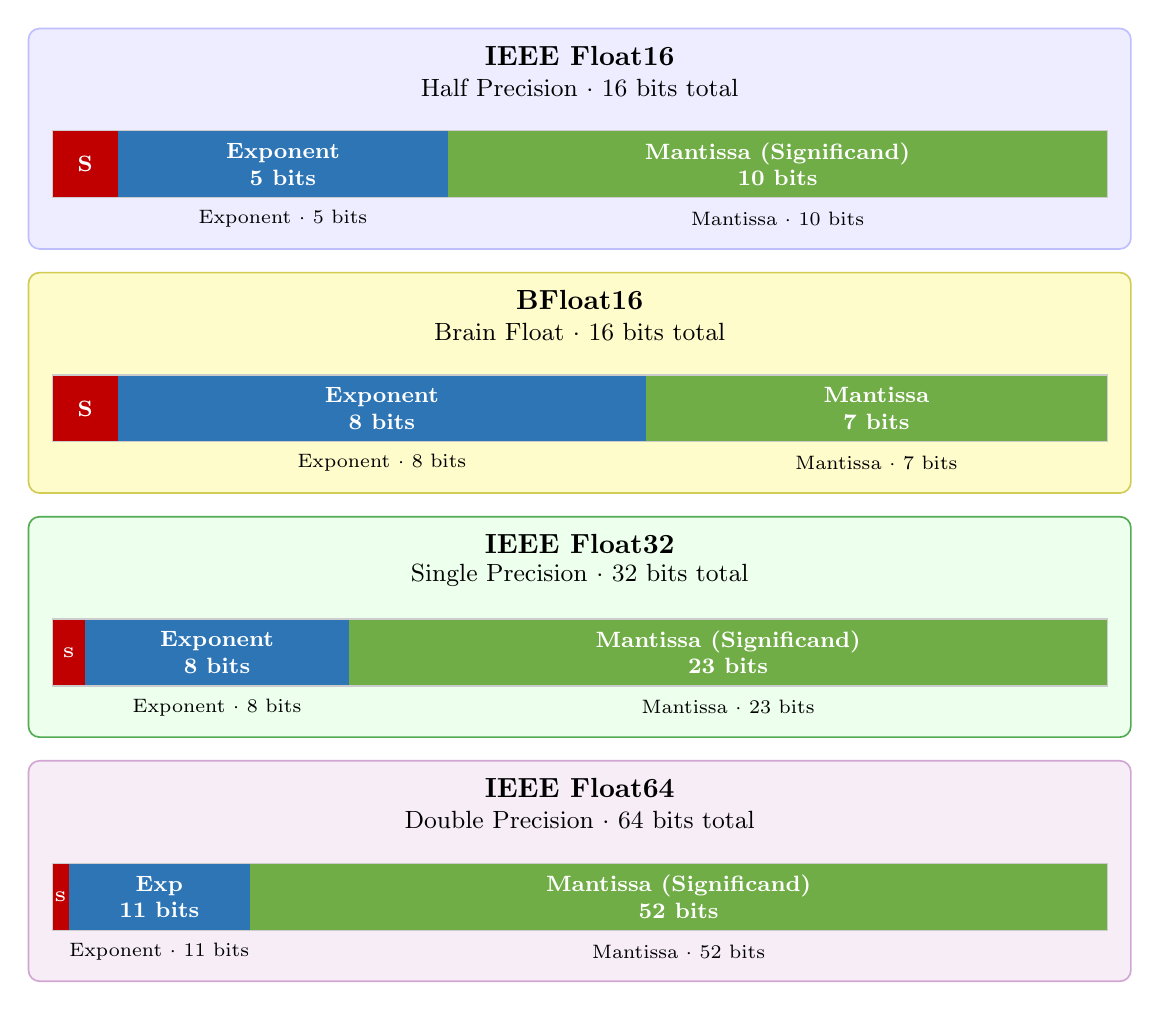
\begin{tikzpicture}[x=1cm, y=1cm]

  % ---- Color palette ----
  \definecolor{signcolor}{RGB}{192,0,0}     % red   -- sign bit
  \definecolor{expcolor} {RGB}{46,117,182}  % blue  -- exponent
  \definecolor{mancolor} {RGB}{112,173,71}  % green -- mantissa

  % ---- Panel backgrounds ----
  % Panels are 14 cm wide x 2.8 cm tall, separated by 0.3 cm gaps.
  % Y positions (bottom edge): Float16=9.30, BFloat16=6.20, Float32=3.10, Float64=0.00
  \draw[rounded corners=4pt, fill=blue!7,    draw=blue!25,        line width=0.6pt]
      (0.0,  9.30) rectangle (14.0, 12.10);  % Float16
  \draw[rounded corners=4pt, fill=yellow!20, draw=yellow!60!gray, line width=0.6pt]
      (0.0,  6.20) rectangle (14.0,  9.00);  % BFloat16
  \draw[rounded corners=4pt, fill=green!7,   draw=green!35!gray,  line width=0.6pt]
      (0.0,  3.10) rectangle (14.0,  5.90);  % Float32
  \draw[rounded corners=4pt, fill=violet!7,  draw=violet!35,      line width=0.6pt]
      (0.0,  0.00) rectangle (14.0,  2.80);  % Float64

  % ====================================================================
  % Bar geometry (shared across all panels):
  %   x range:    [0.30, 13.70]  => total bar width = 13.40 cm
  %   bar height: 0.85 cm
  %   bar bottom: panel_bottom + 0.65
  %   bar top:    panel_bottom + 1.50
  %
  % Segment x boundaries  (width = n_bits/total * 13.40):
  %   Float16  (16-bit): 0.300 | 1.138 | 5.325 | 13.700
  %   BFloat16 (16-bit): 0.300 | 1.138 | 7.838 | 13.700
  %   Float32  (32-bit): 0.300 | 0.719 | 4.069 | 13.700
  %   Float64  (64-bit): 0.300 | 0.509 | 2.813 | 13.700
  % ====================================================================

  % ------------------------------------------------------------------
  % IEEE Float16  (panel bottom y = 9.30)
  % ------------------------------------------------------------------
  \node[font=\normalsize\bfseries] at (7.0, 11.75) {IEEE Float16};
  \node[font=\small]               at (7.0, 11.35) {Half Precision $\cdot$ 16 bits total};

  % S:   1/16 * 13.40 = 0.838 cm   x: 0.300 -- 1.138,  center: 0.719
  \fill[signcolor] (0.300,  9.95) rectangle ( 1.138, 10.80);
  \node[text=white, font=\footnotesize\bfseries] at (0.719, 10.375) {S};

  % Exp: 5/16 * 13.40 = 4.188 cm   x: 1.138 -- 5.325,  center: 3.231
  \fill[expcolor]  (1.138,  9.95) rectangle ( 5.325, 10.80);
  \node[text=white, font=\footnotesize\bfseries, align=center] at (3.231, 10.375)
      {Exponent \\ 5 bits};

  % Man: 10/16 * 13.40 = 8.375 cm  x: 5.325 -- 13.700, center: 9.513
  \fill[mancolor]  (5.325,  9.95) rectangle (13.700, 10.80);
  \node[text=white, font=\footnotesize\bfseries, align=center] at (9.513, 10.375)
      {Mantissa (Significand) \\ 10 bits};

  \draw[black!20, line width=0.4pt] (0.300, 9.95) rectangle (13.700, 10.80);

  \node[font=\scriptsize] at (3.231, 9.68) {Exponent $\cdot$ 5 bits};
  \node[font=\scriptsize] at (9.513, 9.68) {Mantissa $\cdot$ 10 bits};

  % ------------------------------------------------------------------
  % BFloat16  (panel bottom y = 6.20)
  % ------------------------------------------------------------------
  \node[font=\normalsize\bfseries] at (7.0, 8.65) {BFloat16};
  \node[font=\small]               at (7.0, 8.25) {Brain Float $\cdot$ 16 bits total};

  % S:   1/16 * 13.40 = 0.838 cm   x: 0.300 -- 1.138,  center: 0.719
  \fill[signcolor] (0.300,  6.85) rectangle ( 1.138,  7.70);
  \node[text=white, font=\footnotesize\bfseries] at (0.719, 7.275) {S};

  % Exp: 8/16 * 13.40 = 6.700 cm   x: 1.138 -- 7.838,  center: 4.488
  \fill[expcolor]  (1.138,  6.85) rectangle ( 7.838,  7.70);
  \node[text=white, font=\footnotesize\bfseries, align=center] at (4.488, 7.275)
      {Exponent \\ 8 bits};

  % Man: 7/16 * 13.40 = 5.863 cm   x: 7.838 -- 13.700, center: 10.769
  \fill[mancolor]  (7.838,  6.85) rectangle (13.700,  7.70);
  \node[text=white, font=\footnotesize\bfseries, align=center] at (10.769, 7.275)
      {Mantissa \\ 7 bits};

  \draw[black!20, line width=0.4pt] (0.300, 6.85) rectangle (13.700, 7.70);

  \node[font=\scriptsize] at ( 4.488, 6.58) {Exponent $\cdot$ 8 bits};
  \node[font=\scriptsize] at (10.769, 6.58) {Mantissa $\cdot$ 7 bits};

  % ------------------------------------------------------------------
  % IEEE Float32  (panel bottom y = 3.10)
  % ------------------------------------------------------------------
  \node[font=\normalsize\bfseries] at (7.0, 5.55) {IEEE Float32};
  \node[font=\small]               at (7.0, 5.15) {Single Precision $\cdot$ 32 bits total};

  % S:   1/32 * 13.40 = 0.419 cm   x: 0.300 -- 0.719,  center: 0.510
  \fill[signcolor] (0.300,  3.75) rectangle ( 0.719,  4.60);
  \node[text=white, font=\tiny\bfseries] at (0.510, 4.175) {S};

  % Exp: 8/32 * 13.40 = 3.350 cm   x: 0.719 -- 4.069,  center: 2.394
  \fill[expcolor]  (0.719,  3.75) rectangle ( 4.069,  4.60);
  \node[text=white, font=\footnotesize\bfseries, align=center] at (2.394, 4.175)
      {Exponent \\ 8 bits};

  % Man: 23/32 * 13.40 = 9.631 cm  x: 4.069 -- 13.700, center: 8.885
  \fill[mancolor]  (4.069,  3.75) rectangle (13.700,  4.60);
  \node[text=white, font=\footnotesize\bfseries, align=center] at (8.885, 4.175)
      {Mantissa (Significand) \\ 23 bits};

  \draw[black!20, line width=0.4pt] (0.300, 3.75) rectangle (13.700, 4.60);

  \node[font=\scriptsize] at (2.394, 3.48) {Exponent $\cdot$ 8 bits};
  \node[font=\scriptsize] at (8.885, 3.48) {Mantissa $\cdot$ 23 bits};

  % ------------------------------------------------------------------
  % IEEE Float64  (panel bottom y = 0.00)
  % ------------------------------------------------------------------
  \node[font=\normalsize\bfseries] at (7.0, 2.45) {IEEE Float64};
  \node[font=\small]               at (7.0, 2.05) {Double Precision $\cdot$ 64 bits total};

  % S:    1/64 * 13.40 = 0.209 cm  x: 0.300 -- 0.509,  center: 0.405
  \fill[signcolor] (0.300,  0.65) rectangle ( 0.509,  1.50);
  \node[text=white, font=\tiny\bfseries] at (0.405, 1.075) {S};

  % Exp: 11/64 * 13.40 = 2.303 cm  x: 0.509 -- 2.813,  center: 1.661
  \fill[expcolor]  (0.509,  0.65) rectangle ( 2.813,  1.50);
  \node[text=white, font=\footnotesize\bfseries, align=center] at (1.661, 1.075)
      {Exp \\ 11 bits};

  % Man: 52/64 * 13.40 = 10.888 cm x: 2.813 -- 13.700, center: 8.257
  \fill[mancolor]  (2.813,  0.65) rectangle (13.700,  1.50);
  \node[text=white, font=\footnotesize\bfseries, align=center] at (8.257, 1.075)
      {Mantissa (Significand) \\ 52 bits};

  \draw[black!20, line width=0.4pt] (0.300, 0.65) rectangle (13.700, 1.50);

  \node[font=\scriptsize] at (1.661, 0.38) {Exponent $\cdot$ 11 bits};
  \node[font=\scriptsize] at (8.257, 0.38) {Mantissa $\cdot$ 52 bits};

\end{tikzpicture}
}
%
%   Fit to an arbitrary fraction of the column width:
%     \resizebox{0.9\columnwidth}{!}{% Floating-point format comparison — single-column stack layout
%
% Required in preamble:
%   \usepackage{tikz}
%
% ---- Scaling -------------------------------------------------------
% The tikzpicture is drawn at its natural size: 14 cm wide x 12.1 cm tall.
% Use \resizebox (from the graphicx package, always loaded in IEEE style)
% to scale it to whatever width you need. The height adjusts automatically.
%
%   Fit to a single text column (~8.8 cm in IEEE two-column):
%     \resizebox{\columnwidth}{!}{\input{float_formats_tikz.tex}}
%
%   Fit to the full page width (~17.8 cm in IEEE two-column):
%     \resizebox{\textwidth}{!}{\input{float_formats_tikz.tex}}
%
%   Fit to an arbitrary fraction of the column width:
%     \resizebox{0.9\columnwidth}{!}{\input{float_formats_tikz.tex}}
%
% \resizebox scales everything uniformly — coordinates, line widths,
% and fonts — so the result looks identical regardless of the chosen width.
%
% Recommended figure wrapper (single column):
%   \begin{figure}[t]
%     \centering
%     \resizebox{\columnwidth}{!}{\input{float_formats_tikz.tex}}
%     \caption{...}
%     \label{fig:float-formats}
%   \end{figure}
% --------------------------------------------------------------------
%
% Layout: 4 panels stacked vertically, each 14 cm x 2.8 cm.
% Bar widths are proportional to actual bit-field widths.
%   Float16:  S=1, Exp=5,  Man=10  (16 bits total)
%   BFloat16: S=1, Exp=8,  Man=7   (16 bits total)
%   Float32:  S=1, Exp=8,  Man=23  (32 bits total)
%   Float64:  S=1, Exp=11, Man=52  (64 bits total)

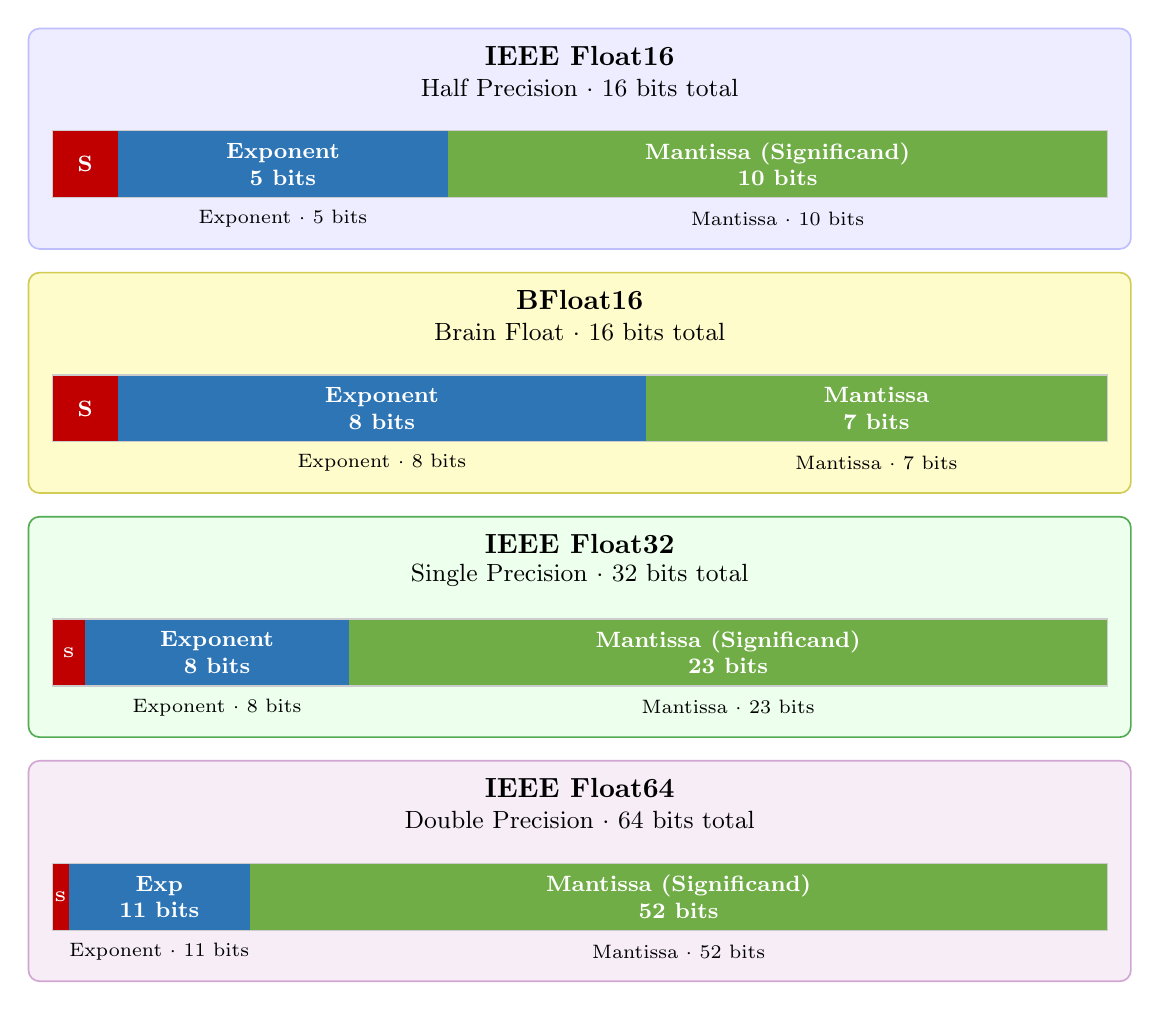
\begin{tikzpicture}[x=1cm, y=1cm]

  % ---- Color palette ----
  \definecolor{signcolor}{RGB}{192,0,0}     % red   -- sign bit
  \definecolor{expcolor} {RGB}{46,117,182}  % blue  -- exponent
  \definecolor{mancolor} {RGB}{112,173,71}  % green -- mantissa

  % ---- Panel backgrounds ----
  % Panels are 14 cm wide x 2.8 cm tall, separated by 0.3 cm gaps.
  % Y positions (bottom edge): Float16=9.30, BFloat16=6.20, Float32=3.10, Float64=0.00
  \draw[rounded corners=4pt, fill=blue!7,    draw=blue!25,        line width=0.6pt]
      (0.0,  9.30) rectangle (14.0, 12.10);  % Float16
  \draw[rounded corners=4pt, fill=yellow!20, draw=yellow!60!gray, line width=0.6pt]
      (0.0,  6.20) rectangle (14.0,  9.00);  % BFloat16
  \draw[rounded corners=4pt, fill=green!7,   draw=green!35!gray,  line width=0.6pt]
      (0.0,  3.10) rectangle (14.0,  5.90);  % Float32
  \draw[rounded corners=4pt, fill=violet!7,  draw=violet!35,      line width=0.6pt]
      (0.0,  0.00) rectangle (14.0,  2.80);  % Float64

  % ====================================================================
  % Bar geometry (shared across all panels):
  %   x range:    [0.30, 13.70]  => total bar width = 13.40 cm
  %   bar height: 0.85 cm
  %   bar bottom: panel_bottom + 0.65
  %   bar top:    panel_bottom + 1.50
  %
  % Segment x boundaries  (width = n_bits/total * 13.40):
  %   Float16  (16-bit): 0.300 | 1.138 | 5.325 | 13.700
  %   BFloat16 (16-bit): 0.300 | 1.138 | 7.838 | 13.700
  %   Float32  (32-bit): 0.300 | 0.719 | 4.069 | 13.700
  %   Float64  (64-bit): 0.300 | 0.509 | 2.813 | 13.700
  % ====================================================================

  % ------------------------------------------------------------------
  % IEEE Float16  (panel bottom y = 9.30)
  % ------------------------------------------------------------------
  \node[font=\normalsize\bfseries] at (7.0, 11.75) {IEEE Float16};
  \node[font=\small]               at (7.0, 11.35) {Half Precision $\cdot$ 16 bits total};

  % S:   1/16 * 13.40 = 0.838 cm   x: 0.300 -- 1.138,  center: 0.719
  \fill[signcolor] (0.300,  9.95) rectangle ( 1.138, 10.80);
  \node[text=white, font=\footnotesize\bfseries] at (0.719, 10.375) {S};

  % Exp: 5/16 * 13.40 = 4.188 cm   x: 1.138 -- 5.325,  center: 3.231
  \fill[expcolor]  (1.138,  9.95) rectangle ( 5.325, 10.80);
  \node[text=white, font=\footnotesize\bfseries, align=center] at (3.231, 10.375)
      {Exponent \\ 5 bits};

  % Man: 10/16 * 13.40 = 8.375 cm  x: 5.325 -- 13.700, center: 9.513
  \fill[mancolor]  (5.325,  9.95) rectangle (13.700, 10.80);
  \node[text=white, font=\footnotesize\bfseries, align=center] at (9.513, 10.375)
      {Mantissa (Significand) \\ 10 bits};

  \draw[black!20, line width=0.4pt] (0.300, 9.95) rectangle (13.700, 10.80);

  \node[font=\scriptsize] at (3.231, 9.68) {Exponent $\cdot$ 5 bits};
  \node[font=\scriptsize] at (9.513, 9.68) {Mantissa $\cdot$ 10 bits};

  % ------------------------------------------------------------------
  % BFloat16  (panel bottom y = 6.20)
  % ------------------------------------------------------------------
  \node[font=\normalsize\bfseries] at (7.0, 8.65) {BFloat16};
  \node[font=\small]               at (7.0, 8.25) {Brain Float $\cdot$ 16 bits total};

  % S:   1/16 * 13.40 = 0.838 cm   x: 0.300 -- 1.138,  center: 0.719
  \fill[signcolor] (0.300,  6.85) rectangle ( 1.138,  7.70);
  \node[text=white, font=\footnotesize\bfseries] at (0.719, 7.275) {S};

  % Exp: 8/16 * 13.40 = 6.700 cm   x: 1.138 -- 7.838,  center: 4.488
  \fill[expcolor]  (1.138,  6.85) rectangle ( 7.838,  7.70);
  \node[text=white, font=\footnotesize\bfseries, align=center] at (4.488, 7.275)
      {Exponent \\ 8 bits};

  % Man: 7/16 * 13.40 = 5.863 cm   x: 7.838 -- 13.700, center: 10.769
  \fill[mancolor]  (7.838,  6.85) rectangle (13.700,  7.70);
  \node[text=white, font=\footnotesize\bfseries, align=center] at (10.769, 7.275)
      {Mantissa \\ 7 bits};

  \draw[black!20, line width=0.4pt] (0.300, 6.85) rectangle (13.700, 7.70);

  \node[font=\scriptsize] at ( 4.488, 6.58) {Exponent $\cdot$ 8 bits};
  \node[font=\scriptsize] at (10.769, 6.58) {Mantissa $\cdot$ 7 bits};

  % ------------------------------------------------------------------
  % IEEE Float32  (panel bottom y = 3.10)
  % ------------------------------------------------------------------
  \node[font=\normalsize\bfseries] at (7.0, 5.55) {IEEE Float32};
  \node[font=\small]               at (7.0, 5.15) {Single Precision $\cdot$ 32 bits total};

  % S:   1/32 * 13.40 = 0.419 cm   x: 0.300 -- 0.719,  center: 0.510
  \fill[signcolor] (0.300,  3.75) rectangle ( 0.719,  4.60);
  \node[text=white, font=\tiny\bfseries] at (0.510, 4.175) {S};

  % Exp: 8/32 * 13.40 = 3.350 cm   x: 0.719 -- 4.069,  center: 2.394
  \fill[expcolor]  (0.719,  3.75) rectangle ( 4.069,  4.60);
  \node[text=white, font=\footnotesize\bfseries, align=center] at (2.394, 4.175)
      {Exponent \\ 8 bits};

  % Man: 23/32 * 13.40 = 9.631 cm  x: 4.069 -- 13.700, center: 8.885
  \fill[mancolor]  (4.069,  3.75) rectangle (13.700,  4.60);
  \node[text=white, font=\footnotesize\bfseries, align=center] at (8.885, 4.175)
      {Mantissa (Significand) \\ 23 bits};

  \draw[black!20, line width=0.4pt] (0.300, 3.75) rectangle (13.700, 4.60);

  \node[font=\scriptsize] at (2.394, 3.48) {Exponent $\cdot$ 8 bits};
  \node[font=\scriptsize] at (8.885, 3.48) {Mantissa $\cdot$ 23 bits};

  % ------------------------------------------------------------------
  % IEEE Float64  (panel bottom y = 0.00)
  % ------------------------------------------------------------------
  \node[font=\normalsize\bfseries] at (7.0, 2.45) {IEEE Float64};
  \node[font=\small]               at (7.0, 2.05) {Double Precision $\cdot$ 64 bits total};

  % S:    1/64 * 13.40 = 0.209 cm  x: 0.300 -- 0.509,  center: 0.405
  \fill[signcolor] (0.300,  0.65) rectangle ( 0.509,  1.50);
  \node[text=white, font=\tiny\bfseries] at (0.405, 1.075) {S};

  % Exp: 11/64 * 13.40 = 2.303 cm  x: 0.509 -- 2.813,  center: 1.661
  \fill[expcolor]  (0.509,  0.65) rectangle ( 2.813,  1.50);
  \node[text=white, font=\footnotesize\bfseries, align=center] at (1.661, 1.075)
      {Exp \\ 11 bits};

  % Man: 52/64 * 13.40 = 10.888 cm x: 2.813 -- 13.700, center: 8.257
  \fill[mancolor]  (2.813,  0.65) rectangle (13.700,  1.50);
  \node[text=white, font=\footnotesize\bfseries, align=center] at (8.257, 1.075)
      {Mantissa (Significand) \\ 52 bits};

  \draw[black!20, line width=0.4pt] (0.300, 0.65) rectangle (13.700, 1.50);

  \node[font=\scriptsize] at (1.661, 0.38) {Exponent $\cdot$ 11 bits};
  \node[font=\scriptsize] at (8.257, 0.38) {Mantissa $\cdot$ 52 bits};

\end{tikzpicture}
}
%
% \resizebox scales everything uniformly — coordinates, line widths,
% and fonts — so the result looks identical regardless of the chosen width.
%
% Recommended figure wrapper (single column):
%   \begin{figure}[t]
%     \centering
%     \resizebox{\columnwidth}{!}{% Floating-point format comparison — single-column stack layout
%
% Required in preamble:
%   \usepackage{tikz}
%
% ---- Scaling -------------------------------------------------------
% The tikzpicture is drawn at its natural size: 14 cm wide x 12.1 cm tall.
% Use \resizebox (from the graphicx package, always loaded in IEEE style)
% to scale it to whatever width you need. The height adjusts automatically.
%
%   Fit to a single text column (~8.8 cm in IEEE two-column):
%     \resizebox{\columnwidth}{!}{\input{float_formats_tikz.tex}}
%
%   Fit to the full page width (~17.8 cm in IEEE two-column):
%     \resizebox{\textwidth}{!}{\input{float_formats_tikz.tex}}
%
%   Fit to an arbitrary fraction of the column width:
%     \resizebox{0.9\columnwidth}{!}{\input{float_formats_tikz.tex}}
%
% \resizebox scales everything uniformly — coordinates, line widths,
% and fonts — so the result looks identical regardless of the chosen width.
%
% Recommended figure wrapper (single column):
%   \begin{figure}[t]
%     \centering
%     \resizebox{\columnwidth}{!}{\input{float_formats_tikz.tex}}
%     \caption{...}
%     \label{fig:float-formats}
%   \end{figure}
% --------------------------------------------------------------------
%
% Layout: 4 panels stacked vertically, each 14 cm x 2.8 cm.
% Bar widths are proportional to actual bit-field widths.
%   Float16:  S=1, Exp=5,  Man=10  (16 bits total)
%   BFloat16: S=1, Exp=8,  Man=7   (16 bits total)
%   Float32:  S=1, Exp=8,  Man=23  (32 bits total)
%   Float64:  S=1, Exp=11, Man=52  (64 bits total)

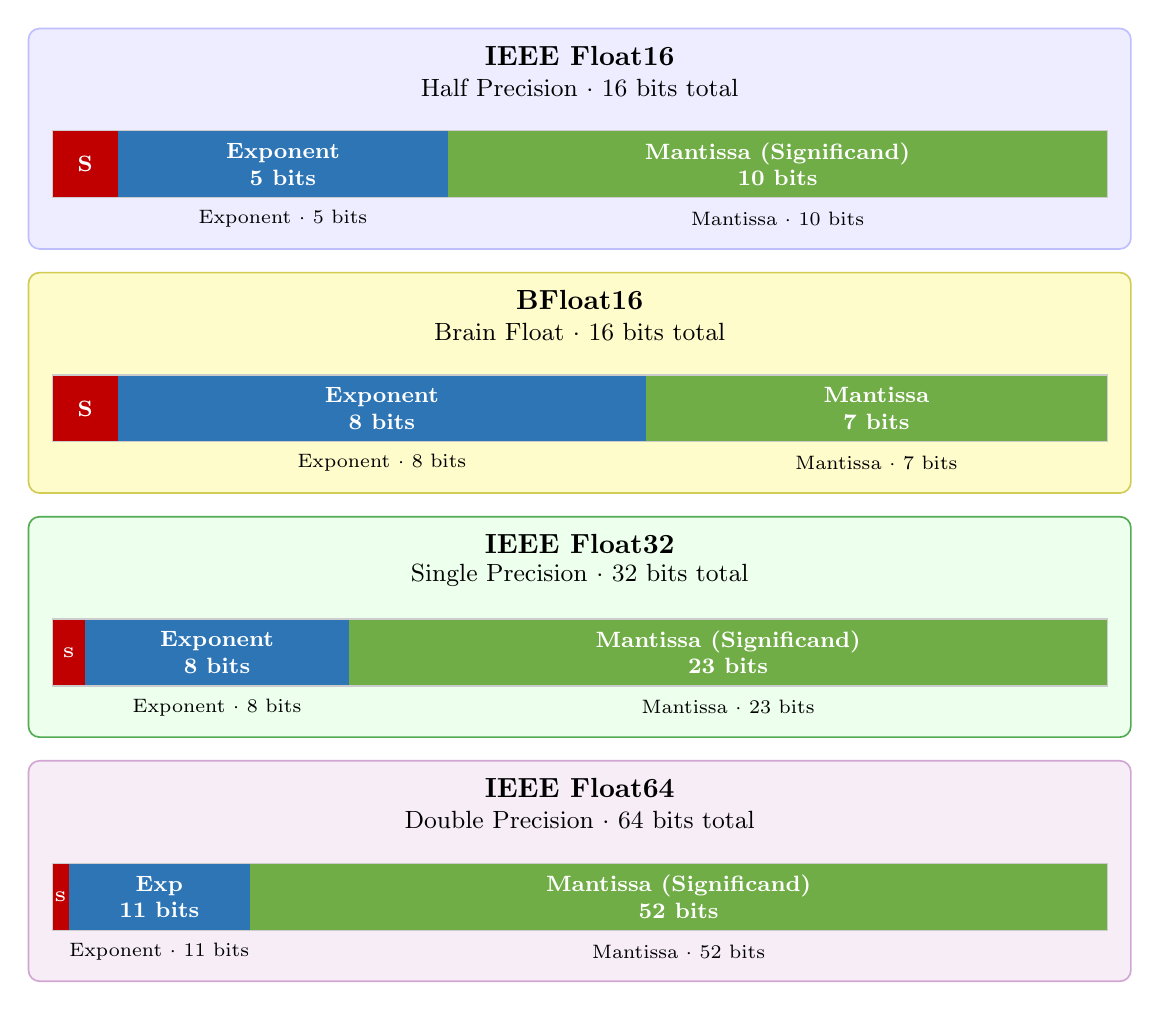
\begin{tikzpicture}[x=1cm, y=1cm]

  % ---- Color palette ----
  \definecolor{signcolor}{RGB}{192,0,0}     % red   -- sign bit
  \definecolor{expcolor} {RGB}{46,117,182}  % blue  -- exponent
  \definecolor{mancolor} {RGB}{112,173,71}  % green -- mantissa

  % ---- Panel backgrounds ----
  % Panels are 14 cm wide x 2.8 cm tall, separated by 0.3 cm gaps.
  % Y positions (bottom edge): Float16=9.30, BFloat16=6.20, Float32=3.10, Float64=0.00
  \draw[rounded corners=4pt, fill=blue!7,    draw=blue!25,        line width=0.6pt]
      (0.0,  9.30) rectangle (14.0, 12.10);  % Float16
  \draw[rounded corners=4pt, fill=yellow!20, draw=yellow!60!gray, line width=0.6pt]
      (0.0,  6.20) rectangle (14.0,  9.00);  % BFloat16
  \draw[rounded corners=4pt, fill=green!7,   draw=green!35!gray,  line width=0.6pt]
      (0.0,  3.10) rectangle (14.0,  5.90);  % Float32
  \draw[rounded corners=4pt, fill=violet!7,  draw=violet!35,      line width=0.6pt]
      (0.0,  0.00) rectangle (14.0,  2.80);  % Float64

  % ====================================================================
  % Bar geometry (shared across all panels):
  %   x range:    [0.30, 13.70]  => total bar width = 13.40 cm
  %   bar height: 0.85 cm
  %   bar bottom: panel_bottom + 0.65
  %   bar top:    panel_bottom + 1.50
  %
  % Segment x boundaries  (width = n_bits/total * 13.40):
  %   Float16  (16-bit): 0.300 | 1.138 | 5.325 | 13.700
  %   BFloat16 (16-bit): 0.300 | 1.138 | 7.838 | 13.700
  %   Float32  (32-bit): 0.300 | 0.719 | 4.069 | 13.700
  %   Float64  (64-bit): 0.300 | 0.509 | 2.813 | 13.700
  % ====================================================================

  % ------------------------------------------------------------------
  % IEEE Float16  (panel bottom y = 9.30)
  % ------------------------------------------------------------------
  \node[font=\normalsize\bfseries] at (7.0, 11.75) {IEEE Float16};
  \node[font=\small]               at (7.0, 11.35) {Half Precision $\cdot$ 16 bits total};

  % S:   1/16 * 13.40 = 0.838 cm   x: 0.300 -- 1.138,  center: 0.719
  \fill[signcolor] (0.300,  9.95) rectangle ( 1.138, 10.80);
  \node[text=white, font=\footnotesize\bfseries] at (0.719, 10.375) {S};

  % Exp: 5/16 * 13.40 = 4.188 cm   x: 1.138 -- 5.325,  center: 3.231
  \fill[expcolor]  (1.138,  9.95) rectangle ( 5.325, 10.80);
  \node[text=white, font=\footnotesize\bfseries, align=center] at (3.231, 10.375)
      {Exponent \\ 5 bits};

  % Man: 10/16 * 13.40 = 8.375 cm  x: 5.325 -- 13.700, center: 9.513
  \fill[mancolor]  (5.325,  9.95) rectangle (13.700, 10.80);
  \node[text=white, font=\footnotesize\bfseries, align=center] at (9.513, 10.375)
      {Mantissa (Significand) \\ 10 bits};

  \draw[black!20, line width=0.4pt] (0.300, 9.95) rectangle (13.700, 10.80);

  \node[font=\scriptsize] at (3.231, 9.68) {Exponent $\cdot$ 5 bits};
  \node[font=\scriptsize] at (9.513, 9.68) {Mantissa $\cdot$ 10 bits};

  % ------------------------------------------------------------------
  % BFloat16  (panel bottom y = 6.20)
  % ------------------------------------------------------------------
  \node[font=\normalsize\bfseries] at (7.0, 8.65) {BFloat16};
  \node[font=\small]               at (7.0, 8.25) {Brain Float $\cdot$ 16 bits total};

  % S:   1/16 * 13.40 = 0.838 cm   x: 0.300 -- 1.138,  center: 0.719
  \fill[signcolor] (0.300,  6.85) rectangle ( 1.138,  7.70);
  \node[text=white, font=\footnotesize\bfseries] at (0.719, 7.275) {S};

  % Exp: 8/16 * 13.40 = 6.700 cm   x: 1.138 -- 7.838,  center: 4.488
  \fill[expcolor]  (1.138,  6.85) rectangle ( 7.838,  7.70);
  \node[text=white, font=\footnotesize\bfseries, align=center] at (4.488, 7.275)
      {Exponent \\ 8 bits};

  % Man: 7/16 * 13.40 = 5.863 cm   x: 7.838 -- 13.700, center: 10.769
  \fill[mancolor]  (7.838,  6.85) rectangle (13.700,  7.70);
  \node[text=white, font=\footnotesize\bfseries, align=center] at (10.769, 7.275)
      {Mantissa \\ 7 bits};

  \draw[black!20, line width=0.4pt] (0.300, 6.85) rectangle (13.700, 7.70);

  \node[font=\scriptsize] at ( 4.488, 6.58) {Exponent $\cdot$ 8 bits};
  \node[font=\scriptsize] at (10.769, 6.58) {Mantissa $\cdot$ 7 bits};

  % ------------------------------------------------------------------
  % IEEE Float32  (panel bottom y = 3.10)
  % ------------------------------------------------------------------
  \node[font=\normalsize\bfseries] at (7.0, 5.55) {IEEE Float32};
  \node[font=\small]               at (7.0, 5.15) {Single Precision $\cdot$ 32 bits total};

  % S:   1/32 * 13.40 = 0.419 cm   x: 0.300 -- 0.719,  center: 0.510
  \fill[signcolor] (0.300,  3.75) rectangle ( 0.719,  4.60);
  \node[text=white, font=\tiny\bfseries] at (0.510, 4.175) {S};

  % Exp: 8/32 * 13.40 = 3.350 cm   x: 0.719 -- 4.069,  center: 2.394
  \fill[expcolor]  (0.719,  3.75) rectangle ( 4.069,  4.60);
  \node[text=white, font=\footnotesize\bfseries, align=center] at (2.394, 4.175)
      {Exponent \\ 8 bits};

  % Man: 23/32 * 13.40 = 9.631 cm  x: 4.069 -- 13.700, center: 8.885
  \fill[mancolor]  (4.069,  3.75) rectangle (13.700,  4.60);
  \node[text=white, font=\footnotesize\bfseries, align=center] at (8.885, 4.175)
      {Mantissa (Significand) \\ 23 bits};

  \draw[black!20, line width=0.4pt] (0.300, 3.75) rectangle (13.700, 4.60);

  \node[font=\scriptsize] at (2.394, 3.48) {Exponent $\cdot$ 8 bits};
  \node[font=\scriptsize] at (8.885, 3.48) {Mantissa $\cdot$ 23 bits};

  % ------------------------------------------------------------------
  % IEEE Float64  (panel bottom y = 0.00)
  % ------------------------------------------------------------------
  \node[font=\normalsize\bfseries] at (7.0, 2.45) {IEEE Float64};
  \node[font=\small]               at (7.0, 2.05) {Double Precision $\cdot$ 64 bits total};

  % S:    1/64 * 13.40 = 0.209 cm  x: 0.300 -- 0.509,  center: 0.405
  \fill[signcolor] (0.300,  0.65) rectangle ( 0.509,  1.50);
  \node[text=white, font=\tiny\bfseries] at (0.405, 1.075) {S};

  % Exp: 11/64 * 13.40 = 2.303 cm  x: 0.509 -- 2.813,  center: 1.661
  \fill[expcolor]  (0.509,  0.65) rectangle ( 2.813,  1.50);
  \node[text=white, font=\footnotesize\bfseries, align=center] at (1.661, 1.075)
      {Exp \\ 11 bits};

  % Man: 52/64 * 13.40 = 10.888 cm x: 2.813 -- 13.700, center: 8.257
  \fill[mancolor]  (2.813,  0.65) rectangle (13.700,  1.50);
  \node[text=white, font=\footnotesize\bfseries, align=center] at (8.257, 1.075)
      {Mantissa (Significand) \\ 52 bits};

  \draw[black!20, line width=0.4pt] (0.300, 0.65) rectangle (13.700, 1.50);

  \node[font=\scriptsize] at (1.661, 0.38) {Exponent $\cdot$ 11 bits};
  \node[font=\scriptsize] at (8.257, 0.38) {Mantissa $\cdot$ 52 bits};

\end{tikzpicture}
}
%     \caption{...}
%     \label{fig:float-formats}
%   \end{figure}
% --------------------------------------------------------------------
%
% Layout: 4 panels stacked vertically, each 14 cm x 2.8 cm.
% Bar widths are proportional to actual bit-field widths.
%   Float16:  S=1, Exp=5,  Man=10  (16 bits total)
%   BFloat16: S=1, Exp=8,  Man=7   (16 bits total)
%   Float32:  S=1, Exp=8,  Man=23  (32 bits total)
%   Float64:  S=1, Exp=11, Man=52  (64 bits total)

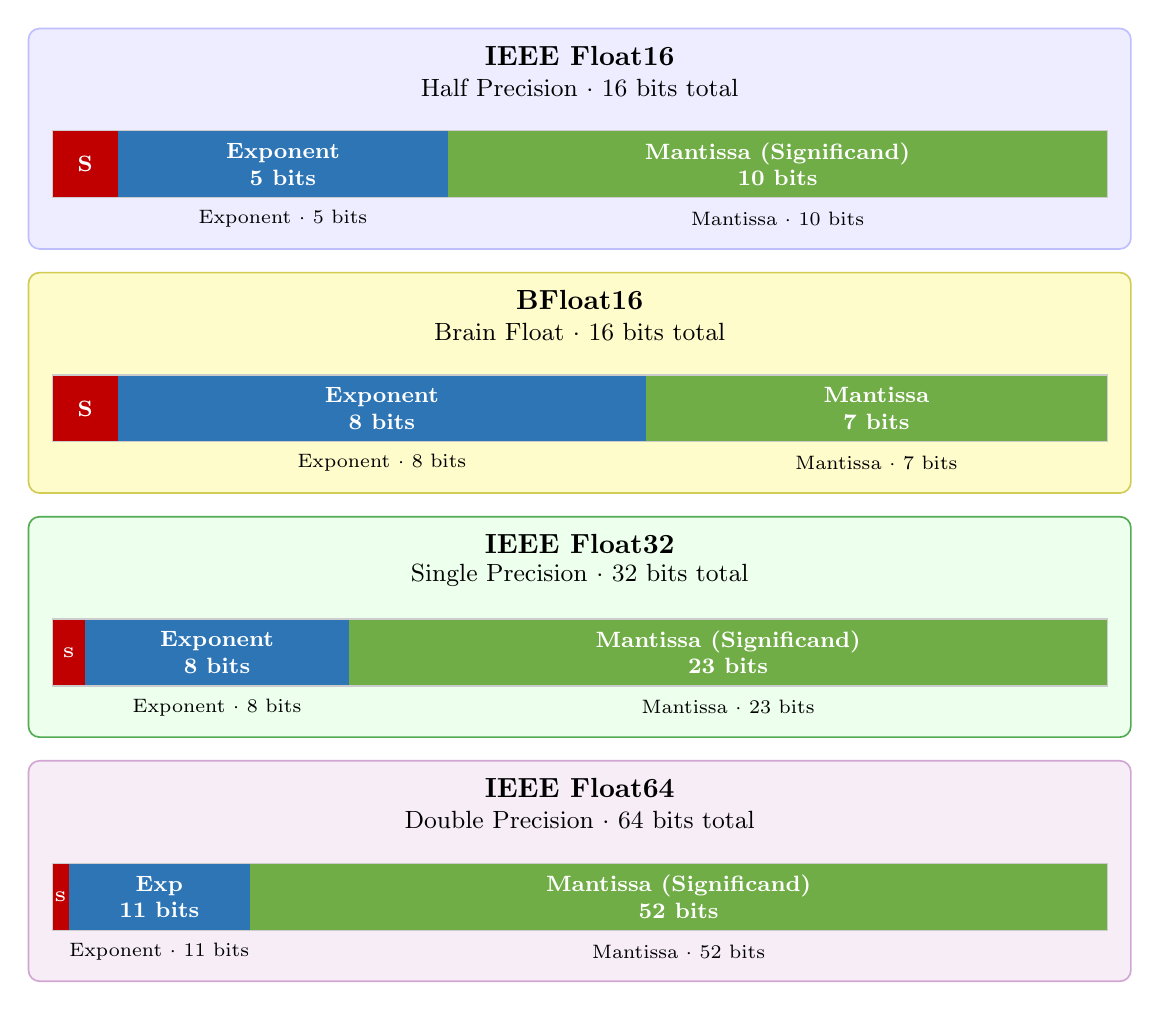
\begin{tikzpicture}[x=1cm, y=1cm]

  % ---- Color palette ----
  \definecolor{signcolor}{RGB}{192,0,0}     % red   -- sign bit
  \definecolor{expcolor} {RGB}{46,117,182}  % blue  -- exponent
  \definecolor{mancolor} {RGB}{112,173,71}  % green -- mantissa

  % ---- Panel backgrounds ----
  % Panels are 14 cm wide x 2.8 cm tall, separated by 0.3 cm gaps.
  % Y positions (bottom edge): Float16=9.30, BFloat16=6.20, Float32=3.10, Float64=0.00
  \draw[rounded corners=4pt, fill=blue!7,    draw=blue!25,        line width=0.6pt]
      (0.0,  9.30) rectangle (14.0, 12.10);  % Float16
  \draw[rounded corners=4pt, fill=yellow!20, draw=yellow!60!gray, line width=0.6pt]
      (0.0,  6.20) rectangle (14.0,  9.00);  % BFloat16
  \draw[rounded corners=4pt, fill=green!7,   draw=green!35!gray,  line width=0.6pt]
      (0.0,  3.10) rectangle (14.0,  5.90);  % Float32
  \draw[rounded corners=4pt, fill=violet!7,  draw=violet!35,      line width=0.6pt]
      (0.0,  0.00) rectangle (14.0,  2.80);  % Float64

  % ====================================================================
  % Bar geometry (shared across all panels):
  %   x range:    [0.30, 13.70]  => total bar width = 13.40 cm
  %   bar height: 0.85 cm
  %   bar bottom: panel_bottom + 0.65
  %   bar top:    panel_bottom + 1.50
  %
  % Segment x boundaries  (width = n_bits/total * 13.40):
  %   Float16  (16-bit): 0.300 | 1.138 | 5.325 | 13.700
  %   BFloat16 (16-bit): 0.300 | 1.138 | 7.838 | 13.700
  %   Float32  (32-bit): 0.300 | 0.719 | 4.069 | 13.700
  %   Float64  (64-bit): 0.300 | 0.509 | 2.813 | 13.700
  % ====================================================================

  % ------------------------------------------------------------------
  % IEEE Float16  (panel bottom y = 9.30)
  % ------------------------------------------------------------------
  \node[font=\normalsize\bfseries] at (7.0, 11.75) {IEEE Float16};
  \node[font=\small]               at (7.0, 11.35) {Half Precision $\cdot$ 16 bits total};

  % S:   1/16 * 13.40 = 0.838 cm   x: 0.300 -- 1.138,  center: 0.719
  \fill[signcolor] (0.300,  9.95) rectangle ( 1.138, 10.80);
  \node[text=white, font=\footnotesize\bfseries] at (0.719, 10.375) {S};

  % Exp: 5/16 * 13.40 = 4.188 cm   x: 1.138 -- 5.325,  center: 3.231
  \fill[expcolor]  (1.138,  9.95) rectangle ( 5.325, 10.80);
  \node[text=white, font=\footnotesize\bfseries, align=center] at (3.231, 10.375)
      {Exponent \\ 5 bits};

  % Man: 10/16 * 13.40 = 8.375 cm  x: 5.325 -- 13.700, center: 9.513
  \fill[mancolor]  (5.325,  9.95) rectangle (13.700, 10.80);
  \node[text=white, font=\footnotesize\bfseries, align=center] at (9.513, 10.375)
      {Mantissa (Significand) \\ 10 bits};

  \draw[black!20, line width=0.4pt] (0.300, 9.95) rectangle (13.700, 10.80);

  \node[font=\scriptsize] at (3.231, 9.68) {Exponent $\cdot$ 5 bits};
  \node[font=\scriptsize] at (9.513, 9.68) {Mantissa $\cdot$ 10 bits};

  % ------------------------------------------------------------------
  % BFloat16  (panel bottom y = 6.20)
  % ------------------------------------------------------------------
  \node[font=\normalsize\bfseries] at (7.0, 8.65) {BFloat16};
  \node[font=\small]               at (7.0, 8.25) {Brain Float $\cdot$ 16 bits total};

  % S:   1/16 * 13.40 = 0.838 cm   x: 0.300 -- 1.138,  center: 0.719
  \fill[signcolor] (0.300,  6.85) rectangle ( 1.138,  7.70);
  \node[text=white, font=\footnotesize\bfseries] at (0.719, 7.275) {S};

  % Exp: 8/16 * 13.40 = 6.700 cm   x: 1.138 -- 7.838,  center: 4.488
  \fill[expcolor]  (1.138,  6.85) rectangle ( 7.838,  7.70);
  \node[text=white, font=\footnotesize\bfseries, align=center] at (4.488, 7.275)
      {Exponent \\ 8 bits};

  % Man: 7/16 * 13.40 = 5.863 cm   x: 7.838 -- 13.700, center: 10.769
  \fill[mancolor]  (7.838,  6.85) rectangle (13.700,  7.70);
  \node[text=white, font=\footnotesize\bfseries, align=center] at (10.769, 7.275)
      {Mantissa \\ 7 bits};

  \draw[black!20, line width=0.4pt] (0.300, 6.85) rectangle (13.700, 7.70);

  \node[font=\scriptsize] at ( 4.488, 6.58) {Exponent $\cdot$ 8 bits};
  \node[font=\scriptsize] at (10.769, 6.58) {Mantissa $\cdot$ 7 bits};

  % ------------------------------------------------------------------
  % IEEE Float32  (panel bottom y = 3.10)
  % ------------------------------------------------------------------
  \node[font=\normalsize\bfseries] at (7.0, 5.55) {IEEE Float32};
  \node[font=\small]               at (7.0, 5.15) {Single Precision $\cdot$ 32 bits total};

  % S:   1/32 * 13.40 = 0.419 cm   x: 0.300 -- 0.719,  center: 0.510
  \fill[signcolor] (0.300,  3.75) rectangle ( 0.719,  4.60);
  \node[text=white, font=\tiny\bfseries] at (0.510, 4.175) {S};

  % Exp: 8/32 * 13.40 = 3.350 cm   x: 0.719 -- 4.069,  center: 2.394
  \fill[expcolor]  (0.719,  3.75) rectangle ( 4.069,  4.60);
  \node[text=white, font=\footnotesize\bfseries, align=center] at (2.394, 4.175)
      {Exponent \\ 8 bits};

  % Man: 23/32 * 13.40 = 9.631 cm  x: 4.069 -- 13.700, center: 8.885
  \fill[mancolor]  (4.069,  3.75) rectangle (13.700,  4.60);
  \node[text=white, font=\footnotesize\bfseries, align=center] at (8.885, 4.175)
      {Mantissa (Significand) \\ 23 bits};

  \draw[black!20, line width=0.4pt] (0.300, 3.75) rectangle (13.700, 4.60);

  \node[font=\scriptsize] at (2.394, 3.48) {Exponent $\cdot$ 8 bits};
  \node[font=\scriptsize] at (8.885, 3.48) {Mantissa $\cdot$ 23 bits};

  % ------------------------------------------------------------------
  % IEEE Float64  (panel bottom y = 0.00)
  % ------------------------------------------------------------------
  \node[font=\normalsize\bfseries] at (7.0, 2.45) {IEEE Float64};
  \node[font=\small]               at (7.0, 2.05) {Double Precision $\cdot$ 64 bits total};

  % S:    1/64 * 13.40 = 0.209 cm  x: 0.300 -- 0.509,  center: 0.405
  \fill[signcolor] (0.300,  0.65) rectangle ( 0.509,  1.50);
  \node[text=white, font=\tiny\bfseries] at (0.405, 1.075) {S};

  % Exp: 11/64 * 13.40 = 2.303 cm  x: 0.509 -- 2.813,  center: 1.661
  \fill[expcolor]  (0.509,  0.65) rectangle ( 2.813,  1.50);
  \node[text=white, font=\footnotesize\bfseries, align=center] at (1.661, 1.075)
      {Exp \\ 11 bits};

  % Man: 52/64 * 13.40 = 10.888 cm x: 2.813 -- 13.700, center: 8.257
  \fill[mancolor]  (2.813,  0.65) rectangle (13.700,  1.50);
  \node[text=white, font=\footnotesize\bfseries, align=center] at (8.257, 1.075)
      {Mantissa (Significand) \\ 52 bits};

  \draw[black!20, line width=0.4pt] (0.300, 0.65) rectangle (13.700, 1.50);

  \node[font=\scriptsize] at (1.661, 0.38) {Exponent $\cdot$ 11 bits};
  \node[font=\scriptsize] at (8.257, 0.38) {Mantissa $\cdot$ 52 bits};

\end{tikzpicture}
}
%     \caption{...}
%     \label{fig:float-formats}
%   \end{figure}
% --------------------------------------------------------------------
%
% Layout: 4 panels stacked vertically, each 14 cm x 2.8 cm.
% Bar widths are proportional to actual bit-field widths.
%   Float16:  S=1, Exp=5,  Man=10  (16 bits total)
%   BFloat16: S=1, Exp=8,  Man=7   (16 bits total)
%   Float32:  S=1, Exp=8,  Man=23  (32 bits total)
%   Float64:  S=1, Exp=11, Man=52  (64 bits total)

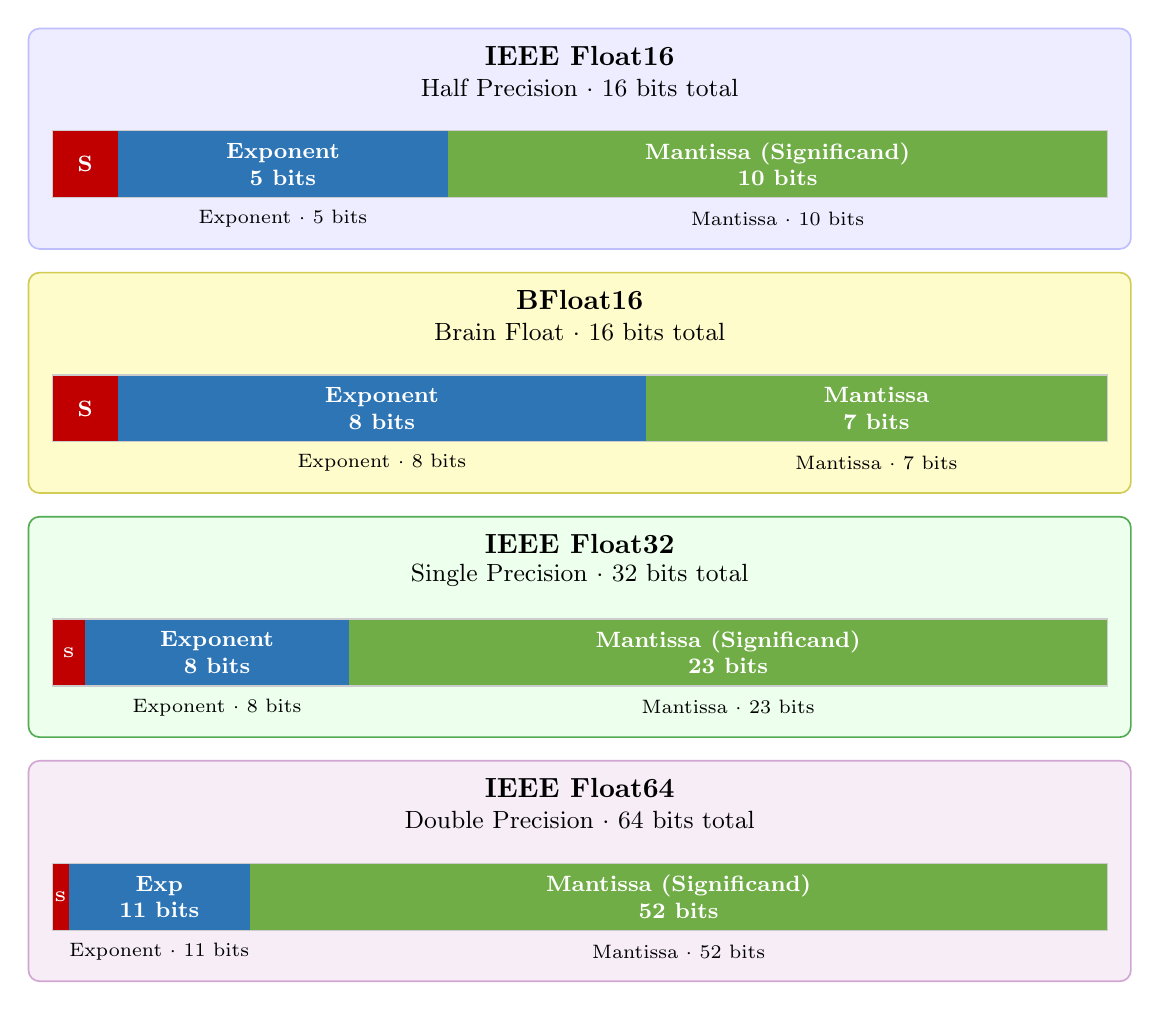
\begin{tikzpicture}[x=1cm, y=1cm]

  % ---- Color palette ----
  \definecolor{signcolor}{RGB}{192,0,0}     % red   -- sign bit
  \definecolor{expcolor} {RGB}{46,117,182}  % blue  -- exponent
  \definecolor{mancolor} {RGB}{112,173,71}  % green -- mantissa

  % ---- Panel backgrounds ----
  % Panels are 14 cm wide x 2.8 cm tall, separated by 0.3 cm gaps.
  % Y positions (bottom edge): Float16=9.30, BFloat16=6.20, Float32=3.10, Float64=0.00
  \draw[rounded corners=4pt, fill=blue!7,    draw=blue!25,        line width=0.6pt]
      (0.0,  9.30) rectangle (14.0, 12.10);  % Float16
  \draw[rounded corners=4pt, fill=yellow!20, draw=yellow!60!gray, line width=0.6pt]
      (0.0,  6.20) rectangle (14.0,  9.00);  % BFloat16
  \draw[rounded corners=4pt, fill=green!7,   draw=green!35!gray,  line width=0.6pt]
      (0.0,  3.10) rectangle (14.0,  5.90);  % Float32
  \draw[rounded corners=4pt, fill=violet!7,  draw=violet!35,      line width=0.6pt]
      (0.0,  0.00) rectangle (14.0,  2.80);  % Float64

  % ====================================================================
  % Bar geometry (shared across all panels):
  %   x range:    [0.30, 13.70]  => total bar width = 13.40 cm
  %   bar height: 0.85 cm
  %   bar bottom: panel_bottom + 0.65
  %   bar top:    panel_bottom + 1.50
  %
  % Segment x boundaries  (width = n_bits/total * 13.40):
  %   Float16  (16-bit): 0.300 | 1.138 | 5.325 | 13.700
  %   BFloat16 (16-bit): 0.300 | 1.138 | 7.838 | 13.700
  %   Float32  (32-bit): 0.300 | 0.719 | 4.069 | 13.700
  %   Float64  (64-bit): 0.300 | 0.509 | 2.813 | 13.700
  % ====================================================================

  % ------------------------------------------------------------------
  % IEEE Float16  (panel bottom y = 9.30)
  % ------------------------------------------------------------------
  \node[font=\normalsize\bfseries] at (7.0, 11.75) {IEEE Float16};
  \node[font=\small]               at (7.0, 11.35) {Half Precision $\cdot$ 16 bits total};

  % S:   1/16 * 13.40 = 0.838 cm   x: 0.300 -- 1.138,  center: 0.719
  \fill[signcolor] (0.300,  9.95) rectangle ( 1.138, 10.80);
  \node[text=white, font=\footnotesize\bfseries] at (0.719, 10.375) {S};

  % Exp: 5/16 * 13.40 = 4.188 cm   x: 1.138 -- 5.325,  center: 3.231
  \fill[expcolor]  (1.138,  9.95) rectangle ( 5.325, 10.80);
  \node[text=white, font=\footnotesize\bfseries, align=center] at (3.231, 10.375)
      {Exponent \\ 5 bits};

  % Man: 10/16 * 13.40 = 8.375 cm  x: 5.325 -- 13.700, center: 9.513
  \fill[mancolor]  (5.325,  9.95) rectangle (13.700, 10.80);
  \node[text=white, font=\footnotesize\bfseries, align=center] at (9.513, 10.375)
      {Mantissa (Significand) \\ 10 bits};

  \draw[black!20, line width=0.4pt] (0.300, 9.95) rectangle (13.700, 10.80);

  \node[font=\scriptsize] at (3.231, 9.68) {Exponent $\cdot$ 5 bits};
  \node[font=\scriptsize] at (9.513, 9.68) {Mantissa $\cdot$ 10 bits};

  % ------------------------------------------------------------------
  % BFloat16  (panel bottom y = 6.20)
  % ------------------------------------------------------------------
  \node[font=\normalsize\bfseries] at (7.0, 8.65) {BFloat16};
  \node[font=\small]               at (7.0, 8.25) {Brain Float $\cdot$ 16 bits total};

  % S:   1/16 * 13.40 = 0.838 cm   x: 0.300 -- 1.138,  center: 0.719
  \fill[signcolor] (0.300,  6.85) rectangle ( 1.138,  7.70);
  \node[text=white, font=\footnotesize\bfseries] at (0.719, 7.275) {S};

  % Exp: 8/16 * 13.40 = 6.700 cm   x: 1.138 -- 7.838,  center: 4.488
  \fill[expcolor]  (1.138,  6.85) rectangle ( 7.838,  7.70);
  \node[text=white, font=\footnotesize\bfseries, align=center] at (4.488, 7.275)
      {Exponent \\ 8 bits};

  % Man: 7/16 * 13.40 = 5.863 cm   x: 7.838 -- 13.700, center: 10.769
  \fill[mancolor]  (7.838,  6.85) rectangle (13.700,  7.70);
  \node[text=white, font=\footnotesize\bfseries, align=center] at (10.769, 7.275)
      {Mantissa \\ 7 bits};

  \draw[black!20, line width=0.4pt] (0.300, 6.85) rectangle (13.700, 7.70);

  \node[font=\scriptsize] at ( 4.488, 6.58) {Exponent $\cdot$ 8 bits};
  \node[font=\scriptsize] at (10.769, 6.58) {Mantissa $\cdot$ 7 bits};

  % ------------------------------------------------------------------
  % IEEE Float32  (panel bottom y = 3.10)
  % ------------------------------------------------------------------
  \node[font=\normalsize\bfseries] at (7.0, 5.55) {IEEE Float32};
  \node[font=\small]               at (7.0, 5.15) {Single Precision $\cdot$ 32 bits total};

  % S:   1/32 * 13.40 = 0.419 cm   x: 0.300 -- 0.719,  center: 0.510
  \fill[signcolor] (0.300,  3.75) rectangle ( 0.719,  4.60);
  \node[text=white, font=\tiny\bfseries] at (0.510, 4.175) {S};

  % Exp: 8/32 * 13.40 = 3.350 cm   x: 0.719 -- 4.069,  center: 2.394
  \fill[expcolor]  (0.719,  3.75) rectangle ( 4.069,  4.60);
  \node[text=white, font=\footnotesize\bfseries, align=center] at (2.394, 4.175)
      {Exponent \\ 8 bits};

  % Man: 23/32 * 13.40 = 9.631 cm  x: 4.069 -- 13.700, center: 8.885
  \fill[mancolor]  (4.069,  3.75) rectangle (13.700,  4.60);
  \node[text=white, font=\footnotesize\bfseries, align=center] at (8.885, 4.175)
      {Mantissa (Significand) \\ 23 bits};

  \draw[black!20, line width=0.4pt] (0.300, 3.75) rectangle (13.700, 4.60);

  \node[font=\scriptsize] at (2.394, 3.48) {Exponent $\cdot$ 8 bits};
  \node[font=\scriptsize] at (8.885, 3.48) {Mantissa $\cdot$ 23 bits};

  % ------------------------------------------------------------------
  % IEEE Float64  (panel bottom y = 0.00)
  % ------------------------------------------------------------------
  \node[font=\normalsize\bfseries] at (7.0, 2.45) {IEEE Float64};
  \node[font=\small]               at (7.0, 2.05) {Double Precision $\cdot$ 64 bits total};

  % S:    1/64 * 13.40 = 0.209 cm  x: 0.300 -- 0.509,  center: 0.405
  \fill[signcolor] (0.300,  0.65) rectangle ( 0.509,  1.50);
  \node[text=white, font=\tiny\bfseries] at (0.405, 1.075) {S};

  % Exp: 11/64 * 13.40 = 2.303 cm  x: 0.509 -- 2.813,  center: 1.661
  \fill[expcolor]  (0.509,  0.65) rectangle ( 2.813,  1.50);
  \node[text=white, font=\footnotesize\bfseries, align=center] at (1.661, 1.075)
      {Exp \\ 11 bits};

  % Man: 52/64 * 13.40 = 10.888 cm x: 2.813 -- 13.700, center: 8.257
  \fill[mancolor]  (2.813,  0.65) rectangle (13.700,  1.50);
  \node[text=white, font=\footnotesize\bfseries, align=center] at (8.257, 1.075)
      {Mantissa (Significand) \\ 52 bits};

  \draw[black!20, line width=0.4pt] (0.300, 0.65) rectangle (13.700, 1.50);

  \node[font=\scriptsize] at (1.661, 0.38) {Exponent $\cdot$ 11 bits};
  \node[font=\scriptsize] at (8.257, 0.38) {Mantissa $\cdot$ 52 bits};

\end{tikzpicture}
}
%
%   Fit to the full page width (~17.8 cm in IEEE two-column):
%     \resizebox{\textwidth}{!}{% Floating-point format comparison — single-column stack layout
%
% Required in preamble:
%   \usepackage{tikz}
%
% ---- Scaling -------------------------------------------------------
% The tikzpicture is drawn at its natural size: 14 cm wide x 12.1 cm tall.
% Use \resizebox (from the graphicx package, always loaded in IEEE style)
% to scale it to whatever width you need. The height adjusts automatically.
%
%   Fit to a single text column (~8.8 cm in IEEE two-column):
%     \resizebox{\columnwidth}{!}{% Floating-point format comparison — single-column stack layout
%
% Required in preamble:
%   \usepackage{tikz}
%
% ---- Scaling -------------------------------------------------------
% The tikzpicture is drawn at its natural size: 14 cm wide x 12.1 cm tall.
% Use \resizebox (from the graphicx package, always loaded in IEEE style)
% to scale it to whatever width you need. The height adjusts automatically.
%
%   Fit to a single text column (~8.8 cm in IEEE two-column):
%     \resizebox{\columnwidth}{!}{% Floating-point format comparison — single-column stack layout
%
% Required in preamble:
%   \usepackage{tikz}
%
% ---- Scaling -------------------------------------------------------
% The tikzpicture is drawn at its natural size: 14 cm wide x 12.1 cm tall.
% Use \resizebox (from the graphicx package, always loaded in IEEE style)
% to scale it to whatever width you need. The height adjusts automatically.
%
%   Fit to a single text column (~8.8 cm in IEEE two-column):
%     \resizebox{\columnwidth}{!}{\input{float_formats_tikz.tex}}
%
%   Fit to the full page width (~17.8 cm in IEEE two-column):
%     \resizebox{\textwidth}{!}{\input{float_formats_tikz.tex}}
%
%   Fit to an arbitrary fraction of the column width:
%     \resizebox{0.9\columnwidth}{!}{\input{float_formats_tikz.tex}}
%
% \resizebox scales everything uniformly — coordinates, line widths,
% and fonts — so the result looks identical regardless of the chosen width.
%
% Recommended figure wrapper (single column):
%   \begin{figure}[t]
%     \centering
%     \resizebox{\columnwidth}{!}{\input{float_formats_tikz.tex}}
%     \caption{...}
%     \label{fig:float-formats}
%   \end{figure}
% --------------------------------------------------------------------
%
% Layout: 4 panels stacked vertically, each 14 cm x 2.8 cm.
% Bar widths are proportional to actual bit-field widths.
%   Float16:  S=1, Exp=5,  Man=10  (16 bits total)
%   BFloat16: S=1, Exp=8,  Man=7   (16 bits total)
%   Float32:  S=1, Exp=8,  Man=23  (32 bits total)
%   Float64:  S=1, Exp=11, Man=52  (64 bits total)

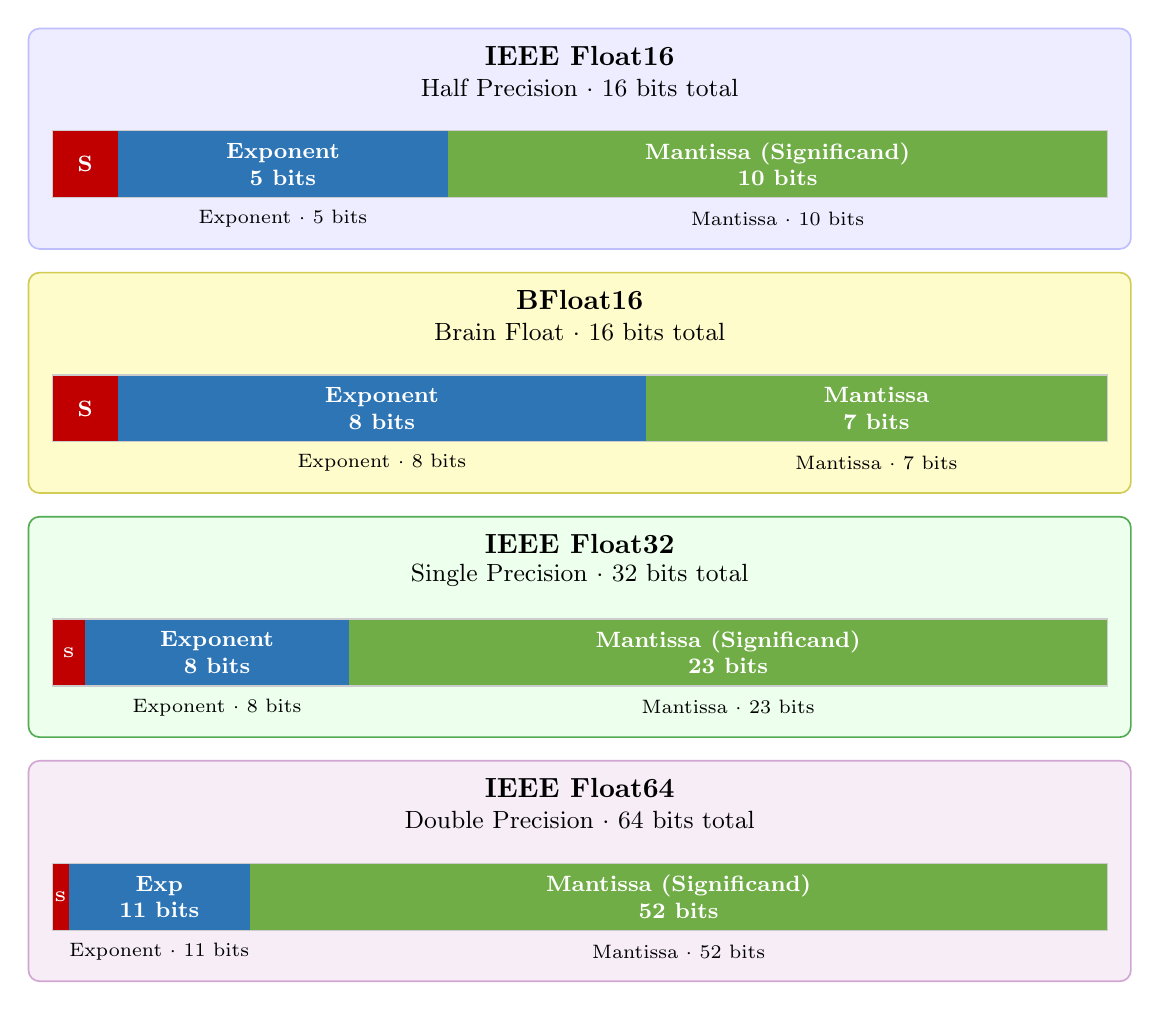
\begin{tikzpicture}[x=1cm, y=1cm]

  % ---- Color palette ----
  \definecolor{signcolor}{RGB}{192,0,0}     % red   -- sign bit
  \definecolor{expcolor} {RGB}{46,117,182}  % blue  -- exponent
  \definecolor{mancolor} {RGB}{112,173,71}  % green -- mantissa

  % ---- Panel backgrounds ----
  % Panels are 14 cm wide x 2.8 cm tall, separated by 0.3 cm gaps.
  % Y positions (bottom edge): Float16=9.30, BFloat16=6.20, Float32=3.10, Float64=0.00
  \draw[rounded corners=4pt, fill=blue!7,    draw=blue!25,        line width=0.6pt]
      (0.0,  9.30) rectangle (14.0, 12.10);  % Float16
  \draw[rounded corners=4pt, fill=yellow!20, draw=yellow!60!gray, line width=0.6pt]
      (0.0,  6.20) rectangle (14.0,  9.00);  % BFloat16
  \draw[rounded corners=4pt, fill=green!7,   draw=green!35!gray,  line width=0.6pt]
      (0.0,  3.10) rectangle (14.0,  5.90);  % Float32
  \draw[rounded corners=4pt, fill=violet!7,  draw=violet!35,      line width=0.6pt]
      (0.0,  0.00) rectangle (14.0,  2.80);  % Float64

  % ====================================================================
  % Bar geometry (shared across all panels):
  %   x range:    [0.30, 13.70]  => total bar width = 13.40 cm
  %   bar height: 0.85 cm
  %   bar bottom: panel_bottom + 0.65
  %   bar top:    panel_bottom + 1.50
  %
  % Segment x boundaries  (width = n_bits/total * 13.40):
  %   Float16  (16-bit): 0.300 | 1.138 | 5.325 | 13.700
  %   BFloat16 (16-bit): 0.300 | 1.138 | 7.838 | 13.700
  %   Float32  (32-bit): 0.300 | 0.719 | 4.069 | 13.700
  %   Float64  (64-bit): 0.300 | 0.509 | 2.813 | 13.700
  % ====================================================================

  % ------------------------------------------------------------------
  % IEEE Float16  (panel bottom y = 9.30)
  % ------------------------------------------------------------------
  \node[font=\normalsize\bfseries] at (7.0, 11.75) {IEEE Float16};
  \node[font=\small]               at (7.0, 11.35) {Half Precision $\cdot$ 16 bits total};

  % S:   1/16 * 13.40 = 0.838 cm   x: 0.300 -- 1.138,  center: 0.719
  \fill[signcolor] (0.300,  9.95) rectangle ( 1.138, 10.80);
  \node[text=white, font=\footnotesize\bfseries] at (0.719, 10.375) {S};

  % Exp: 5/16 * 13.40 = 4.188 cm   x: 1.138 -- 5.325,  center: 3.231
  \fill[expcolor]  (1.138,  9.95) rectangle ( 5.325, 10.80);
  \node[text=white, font=\footnotesize\bfseries, align=center] at (3.231, 10.375)
      {Exponent \\ 5 bits};

  % Man: 10/16 * 13.40 = 8.375 cm  x: 5.325 -- 13.700, center: 9.513
  \fill[mancolor]  (5.325,  9.95) rectangle (13.700, 10.80);
  \node[text=white, font=\footnotesize\bfseries, align=center] at (9.513, 10.375)
      {Mantissa (Significand) \\ 10 bits};

  \draw[black!20, line width=0.4pt] (0.300, 9.95) rectangle (13.700, 10.80);

  \node[font=\scriptsize] at (3.231, 9.68) {Exponent $\cdot$ 5 bits};
  \node[font=\scriptsize] at (9.513, 9.68) {Mantissa $\cdot$ 10 bits};

  % ------------------------------------------------------------------
  % BFloat16  (panel bottom y = 6.20)
  % ------------------------------------------------------------------
  \node[font=\normalsize\bfseries] at (7.0, 8.65) {BFloat16};
  \node[font=\small]               at (7.0, 8.25) {Brain Float $\cdot$ 16 bits total};

  % S:   1/16 * 13.40 = 0.838 cm   x: 0.300 -- 1.138,  center: 0.719
  \fill[signcolor] (0.300,  6.85) rectangle ( 1.138,  7.70);
  \node[text=white, font=\footnotesize\bfseries] at (0.719, 7.275) {S};

  % Exp: 8/16 * 13.40 = 6.700 cm   x: 1.138 -- 7.838,  center: 4.488
  \fill[expcolor]  (1.138,  6.85) rectangle ( 7.838,  7.70);
  \node[text=white, font=\footnotesize\bfseries, align=center] at (4.488, 7.275)
      {Exponent \\ 8 bits};

  % Man: 7/16 * 13.40 = 5.863 cm   x: 7.838 -- 13.700, center: 10.769
  \fill[mancolor]  (7.838,  6.85) rectangle (13.700,  7.70);
  \node[text=white, font=\footnotesize\bfseries, align=center] at (10.769, 7.275)
      {Mantissa \\ 7 bits};

  \draw[black!20, line width=0.4pt] (0.300, 6.85) rectangle (13.700, 7.70);

  \node[font=\scriptsize] at ( 4.488, 6.58) {Exponent $\cdot$ 8 bits};
  \node[font=\scriptsize] at (10.769, 6.58) {Mantissa $\cdot$ 7 bits};

  % ------------------------------------------------------------------
  % IEEE Float32  (panel bottom y = 3.10)
  % ------------------------------------------------------------------
  \node[font=\normalsize\bfseries] at (7.0, 5.55) {IEEE Float32};
  \node[font=\small]               at (7.0, 5.15) {Single Precision $\cdot$ 32 bits total};

  % S:   1/32 * 13.40 = 0.419 cm   x: 0.300 -- 0.719,  center: 0.510
  \fill[signcolor] (0.300,  3.75) rectangle ( 0.719,  4.60);
  \node[text=white, font=\tiny\bfseries] at (0.510, 4.175) {S};

  % Exp: 8/32 * 13.40 = 3.350 cm   x: 0.719 -- 4.069,  center: 2.394
  \fill[expcolor]  (0.719,  3.75) rectangle ( 4.069,  4.60);
  \node[text=white, font=\footnotesize\bfseries, align=center] at (2.394, 4.175)
      {Exponent \\ 8 bits};

  % Man: 23/32 * 13.40 = 9.631 cm  x: 4.069 -- 13.700, center: 8.885
  \fill[mancolor]  (4.069,  3.75) rectangle (13.700,  4.60);
  \node[text=white, font=\footnotesize\bfseries, align=center] at (8.885, 4.175)
      {Mantissa (Significand) \\ 23 bits};

  \draw[black!20, line width=0.4pt] (0.300, 3.75) rectangle (13.700, 4.60);

  \node[font=\scriptsize] at (2.394, 3.48) {Exponent $\cdot$ 8 bits};
  \node[font=\scriptsize] at (8.885, 3.48) {Mantissa $\cdot$ 23 bits};

  % ------------------------------------------------------------------
  % IEEE Float64  (panel bottom y = 0.00)
  % ------------------------------------------------------------------
  \node[font=\normalsize\bfseries] at (7.0, 2.45) {IEEE Float64};
  \node[font=\small]               at (7.0, 2.05) {Double Precision $\cdot$ 64 bits total};

  % S:    1/64 * 13.40 = 0.209 cm  x: 0.300 -- 0.509,  center: 0.405
  \fill[signcolor] (0.300,  0.65) rectangle ( 0.509,  1.50);
  \node[text=white, font=\tiny\bfseries] at (0.405, 1.075) {S};

  % Exp: 11/64 * 13.40 = 2.303 cm  x: 0.509 -- 2.813,  center: 1.661
  \fill[expcolor]  (0.509,  0.65) rectangle ( 2.813,  1.50);
  \node[text=white, font=\footnotesize\bfseries, align=center] at (1.661, 1.075)
      {Exp \\ 11 bits};

  % Man: 52/64 * 13.40 = 10.888 cm x: 2.813 -- 13.700, center: 8.257
  \fill[mancolor]  (2.813,  0.65) rectangle (13.700,  1.50);
  \node[text=white, font=\footnotesize\bfseries, align=center] at (8.257, 1.075)
      {Mantissa (Significand) \\ 52 bits};

  \draw[black!20, line width=0.4pt] (0.300, 0.65) rectangle (13.700, 1.50);

  \node[font=\scriptsize] at (1.661, 0.38) {Exponent $\cdot$ 11 bits};
  \node[font=\scriptsize] at (8.257, 0.38) {Mantissa $\cdot$ 52 bits};

\end{tikzpicture}
}
%
%   Fit to the full page width (~17.8 cm in IEEE two-column):
%     \resizebox{\textwidth}{!}{% Floating-point format comparison — single-column stack layout
%
% Required in preamble:
%   \usepackage{tikz}
%
% ---- Scaling -------------------------------------------------------
% The tikzpicture is drawn at its natural size: 14 cm wide x 12.1 cm tall.
% Use \resizebox (from the graphicx package, always loaded in IEEE style)
% to scale it to whatever width you need. The height adjusts automatically.
%
%   Fit to a single text column (~8.8 cm in IEEE two-column):
%     \resizebox{\columnwidth}{!}{\input{float_formats_tikz.tex}}
%
%   Fit to the full page width (~17.8 cm in IEEE two-column):
%     \resizebox{\textwidth}{!}{\input{float_formats_tikz.tex}}
%
%   Fit to an arbitrary fraction of the column width:
%     \resizebox{0.9\columnwidth}{!}{\input{float_formats_tikz.tex}}
%
% \resizebox scales everything uniformly — coordinates, line widths,
% and fonts — so the result looks identical regardless of the chosen width.
%
% Recommended figure wrapper (single column):
%   \begin{figure}[t]
%     \centering
%     \resizebox{\columnwidth}{!}{\input{float_formats_tikz.tex}}
%     \caption{...}
%     \label{fig:float-formats}
%   \end{figure}
% --------------------------------------------------------------------
%
% Layout: 4 panels stacked vertically, each 14 cm x 2.8 cm.
% Bar widths are proportional to actual bit-field widths.
%   Float16:  S=1, Exp=5,  Man=10  (16 bits total)
%   BFloat16: S=1, Exp=8,  Man=7   (16 bits total)
%   Float32:  S=1, Exp=8,  Man=23  (32 bits total)
%   Float64:  S=1, Exp=11, Man=52  (64 bits total)

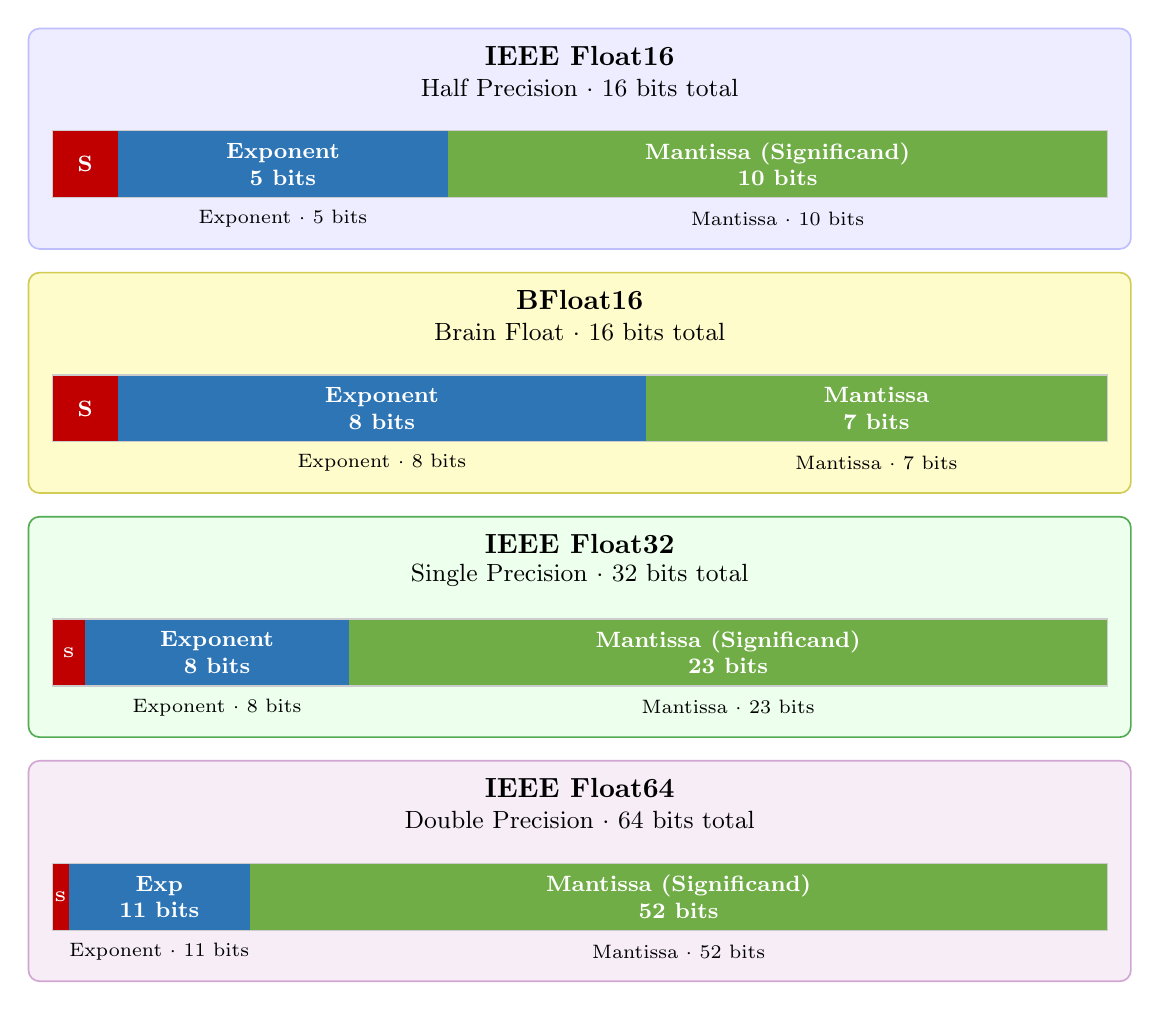
\begin{tikzpicture}[x=1cm, y=1cm]

  % ---- Color palette ----
  \definecolor{signcolor}{RGB}{192,0,0}     % red   -- sign bit
  \definecolor{expcolor} {RGB}{46,117,182}  % blue  -- exponent
  \definecolor{mancolor} {RGB}{112,173,71}  % green -- mantissa

  % ---- Panel backgrounds ----
  % Panels are 14 cm wide x 2.8 cm tall, separated by 0.3 cm gaps.
  % Y positions (bottom edge): Float16=9.30, BFloat16=6.20, Float32=3.10, Float64=0.00
  \draw[rounded corners=4pt, fill=blue!7,    draw=blue!25,        line width=0.6pt]
      (0.0,  9.30) rectangle (14.0, 12.10);  % Float16
  \draw[rounded corners=4pt, fill=yellow!20, draw=yellow!60!gray, line width=0.6pt]
      (0.0,  6.20) rectangle (14.0,  9.00);  % BFloat16
  \draw[rounded corners=4pt, fill=green!7,   draw=green!35!gray,  line width=0.6pt]
      (0.0,  3.10) rectangle (14.0,  5.90);  % Float32
  \draw[rounded corners=4pt, fill=violet!7,  draw=violet!35,      line width=0.6pt]
      (0.0,  0.00) rectangle (14.0,  2.80);  % Float64

  % ====================================================================
  % Bar geometry (shared across all panels):
  %   x range:    [0.30, 13.70]  => total bar width = 13.40 cm
  %   bar height: 0.85 cm
  %   bar bottom: panel_bottom + 0.65
  %   bar top:    panel_bottom + 1.50
  %
  % Segment x boundaries  (width = n_bits/total * 13.40):
  %   Float16  (16-bit): 0.300 | 1.138 | 5.325 | 13.700
  %   BFloat16 (16-bit): 0.300 | 1.138 | 7.838 | 13.700
  %   Float32  (32-bit): 0.300 | 0.719 | 4.069 | 13.700
  %   Float64  (64-bit): 0.300 | 0.509 | 2.813 | 13.700
  % ====================================================================

  % ------------------------------------------------------------------
  % IEEE Float16  (panel bottom y = 9.30)
  % ------------------------------------------------------------------
  \node[font=\normalsize\bfseries] at (7.0, 11.75) {IEEE Float16};
  \node[font=\small]               at (7.0, 11.35) {Half Precision $\cdot$ 16 bits total};

  % S:   1/16 * 13.40 = 0.838 cm   x: 0.300 -- 1.138,  center: 0.719
  \fill[signcolor] (0.300,  9.95) rectangle ( 1.138, 10.80);
  \node[text=white, font=\footnotesize\bfseries] at (0.719, 10.375) {S};

  % Exp: 5/16 * 13.40 = 4.188 cm   x: 1.138 -- 5.325,  center: 3.231
  \fill[expcolor]  (1.138,  9.95) rectangle ( 5.325, 10.80);
  \node[text=white, font=\footnotesize\bfseries, align=center] at (3.231, 10.375)
      {Exponent \\ 5 bits};

  % Man: 10/16 * 13.40 = 8.375 cm  x: 5.325 -- 13.700, center: 9.513
  \fill[mancolor]  (5.325,  9.95) rectangle (13.700, 10.80);
  \node[text=white, font=\footnotesize\bfseries, align=center] at (9.513, 10.375)
      {Mantissa (Significand) \\ 10 bits};

  \draw[black!20, line width=0.4pt] (0.300, 9.95) rectangle (13.700, 10.80);

  \node[font=\scriptsize] at (3.231, 9.68) {Exponent $\cdot$ 5 bits};
  \node[font=\scriptsize] at (9.513, 9.68) {Mantissa $\cdot$ 10 bits};

  % ------------------------------------------------------------------
  % BFloat16  (panel bottom y = 6.20)
  % ------------------------------------------------------------------
  \node[font=\normalsize\bfseries] at (7.0, 8.65) {BFloat16};
  \node[font=\small]               at (7.0, 8.25) {Brain Float $\cdot$ 16 bits total};

  % S:   1/16 * 13.40 = 0.838 cm   x: 0.300 -- 1.138,  center: 0.719
  \fill[signcolor] (0.300,  6.85) rectangle ( 1.138,  7.70);
  \node[text=white, font=\footnotesize\bfseries] at (0.719, 7.275) {S};

  % Exp: 8/16 * 13.40 = 6.700 cm   x: 1.138 -- 7.838,  center: 4.488
  \fill[expcolor]  (1.138,  6.85) rectangle ( 7.838,  7.70);
  \node[text=white, font=\footnotesize\bfseries, align=center] at (4.488, 7.275)
      {Exponent \\ 8 bits};

  % Man: 7/16 * 13.40 = 5.863 cm   x: 7.838 -- 13.700, center: 10.769
  \fill[mancolor]  (7.838,  6.85) rectangle (13.700,  7.70);
  \node[text=white, font=\footnotesize\bfseries, align=center] at (10.769, 7.275)
      {Mantissa \\ 7 bits};

  \draw[black!20, line width=0.4pt] (0.300, 6.85) rectangle (13.700, 7.70);

  \node[font=\scriptsize] at ( 4.488, 6.58) {Exponent $\cdot$ 8 bits};
  \node[font=\scriptsize] at (10.769, 6.58) {Mantissa $\cdot$ 7 bits};

  % ------------------------------------------------------------------
  % IEEE Float32  (panel bottom y = 3.10)
  % ------------------------------------------------------------------
  \node[font=\normalsize\bfseries] at (7.0, 5.55) {IEEE Float32};
  \node[font=\small]               at (7.0, 5.15) {Single Precision $\cdot$ 32 bits total};

  % S:   1/32 * 13.40 = 0.419 cm   x: 0.300 -- 0.719,  center: 0.510
  \fill[signcolor] (0.300,  3.75) rectangle ( 0.719,  4.60);
  \node[text=white, font=\tiny\bfseries] at (0.510, 4.175) {S};

  % Exp: 8/32 * 13.40 = 3.350 cm   x: 0.719 -- 4.069,  center: 2.394
  \fill[expcolor]  (0.719,  3.75) rectangle ( 4.069,  4.60);
  \node[text=white, font=\footnotesize\bfseries, align=center] at (2.394, 4.175)
      {Exponent \\ 8 bits};

  % Man: 23/32 * 13.40 = 9.631 cm  x: 4.069 -- 13.700, center: 8.885
  \fill[mancolor]  (4.069,  3.75) rectangle (13.700,  4.60);
  \node[text=white, font=\footnotesize\bfseries, align=center] at (8.885, 4.175)
      {Mantissa (Significand) \\ 23 bits};

  \draw[black!20, line width=0.4pt] (0.300, 3.75) rectangle (13.700, 4.60);

  \node[font=\scriptsize] at (2.394, 3.48) {Exponent $\cdot$ 8 bits};
  \node[font=\scriptsize] at (8.885, 3.48) {Mantissa $\cdot$ 23 bits};

  % ------------------------------------------------------------------
  % IEEE Float64  (panel bottom y = 0.00)
  % ------------------------------------------------------------------
  \node[font=\normalsize\bfseries] at (7.0, 2.45) {IEEE Float64};
  \node[font=\small]               at (7.0, 2.05) {Double Precision $\cdot$ 64 bits total};

  % S:    1/64 * 13.40 = 0.209 cm  x: 0.300 -- 0.509,  center: 0.405
  \fill[signcolor] (0.300,  0.65) rectangle ( 0.509,  1.50);
  \node[text=white, font=\tiny\bfseries] at (0.405, 1.075) {S};

  % Exp: 11/64 * 13.40 = 2.303 cm  x: 0.509 -- 2.813,  center: 1.661
  \fill[expcolor]  (0.509,  0.65) rectangle ( 2.813,  1.50);
  \node[text=white, font=\footnotesize\bfseries, align=center] at (1.661, 1.075)
      {Exp \\ 11 bits};

  % Man: 52/64 * 13.40 = 10.888 cm x: 2.813 -- 13.700, center: 8.257
  \fill[mancolor]  (2.813,  0.65) rectangle (13.700,  1.50);
  \node[text=white, font=\footnotesize\bfseries, align=center] at (8.257, 1.075)
      {Mantissa (Significand) \\ 52 bits};

  \draw[black!20, line width=0.4pt] (0.300, 0.65) rectangle (13.700, 1.50);

  \node[font=\scriptsize] at (1.661, 0.38) {Exponent $\cdot$ 11 bits};
  \node[font=\scriptsize] at (8.257, 0.38) {Mantissa $\cdot$ 52 bits};

\end{tikzpicture}
}
%
%   Fit to an arbitrary fraction of the column width:
%     \resizebox{0.9\columnwidth}{!}{% Floating-point format comparison — single-column stack layout
%
% Required in preamble:
%   \usepackage{tikz}
%
% ---- Scaling -------------------------------------------------------
% The tikzpicture is drawn at its natural size: 14 cm wide x 12.1 cm tall.
% Use \resizebox (from the graphicx package, always loaded in IEEE style)
% to scale it to whatever width you need. The height adjusts automatically.
%
%   Fit to a single text column (~8.8 cm in IEEE two-column):
%     \resizebox{\columnwidth}{!}{\input{float_formats_tikz.tex}}
%
%   Fit to the full page width (~17.8 cm in IEEE two-column):
%     \resizebox{\textwidth}{!}{\input{float_formats_tikz.tex}}
%
%   Fit to an arbitrary fraction of the column width:
%     \resizebox{0.9\columnwidth}{!}{\input{float_formats_tikz.tex}}
%
% \resizebox scales everything uniformly — coordinates, line widths,
% and fonts — so the result looks identical regardless of the chosen width.
%
% Recommended figure wrapper (single column):
%   \begin{figure}[t]
%     \centering
%     \resizebox{\columnwidth}{!}{\input{float_formats_tikz.tex}}
%     \caption{...}
%     \label{fig:float-formats}
%   \end{figure}
% --------------------------------------------------------------------
%
% Layout: 4 panels stacked vertically, each 14 cm x 2.8 cm.
% Bar widths are proportional to actual bit-field widths.
%   Float16:  S=1, Exp=5,  Man=10  (16 bits total)
%   BFloat16: S=1, Exp=8,  Man=7   (16 bits total)
%   Float32:  S=1, Exp=8,  Man=23  (32 bits total)
%   Float64:  S=1, Exp=11, Man=52  (64 bits total)

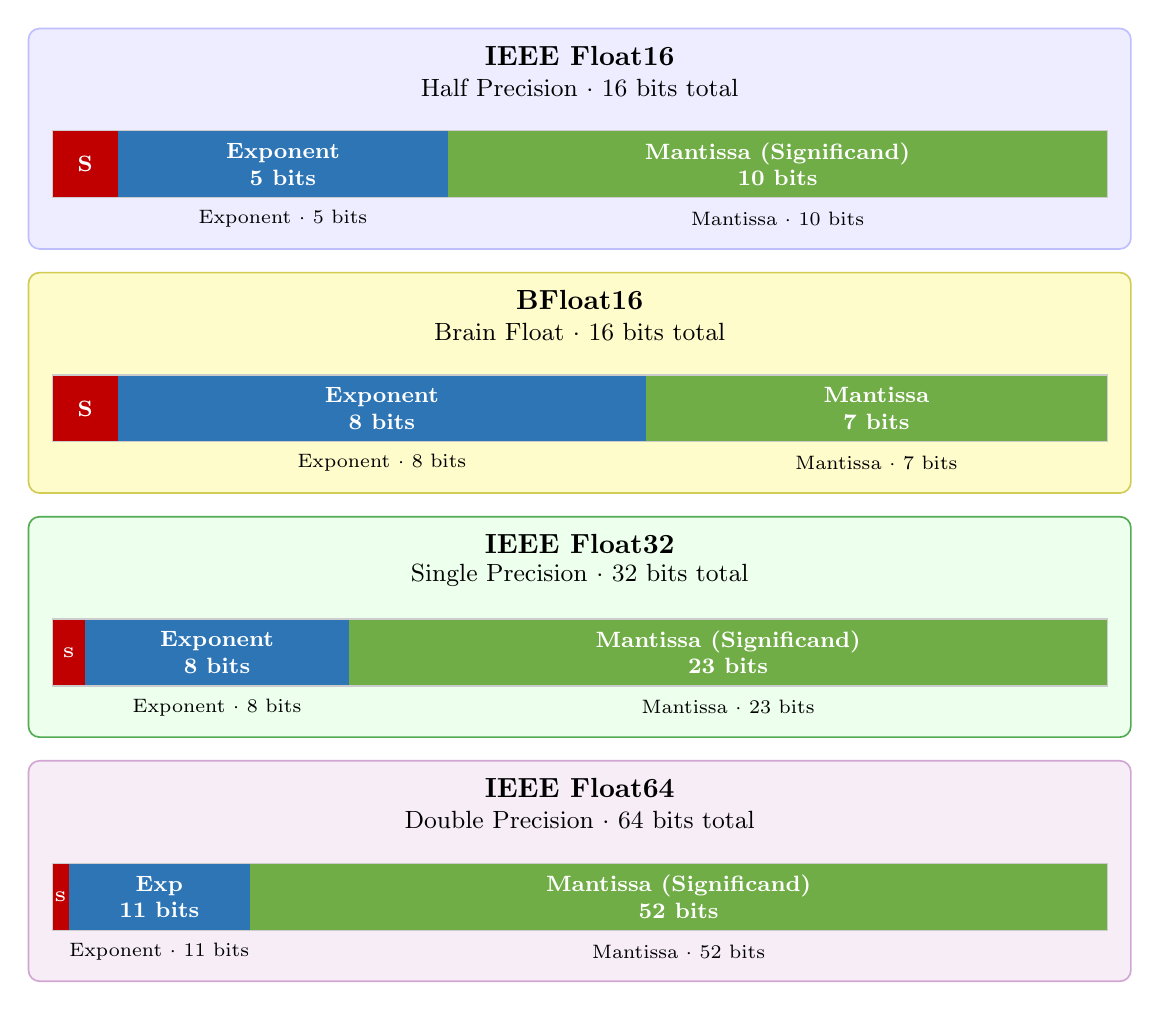
\begin{tikzpicture}[x=1cm, y=1cm]

  % ---- Color palette ----
  \definecolor{signcolor}{RGB}{192,0,0}     % red   -- sign bit
  \definecolor{expcolor} {RGB}{46,117,182}  % blue  -- exponent
  \definecolor{mancolor} {RGB}{112,173,71}  % green -- mantissa

  % ---- Panel backgrounds ----
  % Panels are 14 cm wide x 2.8 cm tall, separated by 0.3 cm gaps.
  % Y positions (bottom edge): Float16=9.30, BFloat16=6.20, Float32=3.10, Float64=0.00
  \draw[rounded corners=4pt, fill=blue!7,    draw=blue!25,        line width=0.6pt]
      (0.0,  9.30) rectangle (14.0, 12.10);  % Float16
  \draw[rounded corners=4pt, fill=yellow!20, draw=yellow!60!gray, line width=0.6pt]
      (0.0,  6.20) rectangle (14.0,  9.00);  % BFloat16
  \draw[rounded corners=4pt, fill=green!7,   draw=green!35!gray,  line width=0.6pt]
      (0.0,  3.10) rectangle (14.0,  5.90);  % Float32
  \draw[rounded corners=4pt, fill=violet!7,  draw=violet!35,      line width=0.6pt]
      (0.0,  0.00) rectangle (14.0,  2.80);  % Float64

  % ====================================================================
  % Bar geometry (shared across all panels):
  %   x range:    [0.30, 13.70]  => total bar width = 13.40 cm
  %   bar height: 0.85 cm
  %   bar bottom: panel_bottom + 0.65
  %   bar top:    panel_bottom + 1.50
  %
  % Segment x boundaries  (width = n_bits/total * 13.40):
  %   Float16  (16-bit): 0.300 | 1.138 | 5.325 | 13.700
  %   BFloat16 (16-bit): 0.300 | 1.138 | 7.838 | 13.700
  %   Float32  (32-bit): 0.300 | 0.719 | 4.069 | 13.700
  %   Float64  (64-bit): 0.300 | 0.509 | 2.813 | 13.700
  % ====================================================================

  % ------------------------------------------------------------------
  % IEEE Float16  (panel bottom y = 9.30)
  % ------------------------------------------------------------------
  \node[font=\normalsize\bfseries] at (7.0, 11.75) {IEEE Float16};
  \node[font=\small]               at (7.0, 11.35) {Half Precision $\cdot$ 16 bits total};

  % S:   1/16 * 13.40 = 0.838 cm   x: 0.300 -- 1.138,  center: 0.719
  \fill[signcolor] (0.300,  9.95) rectangle ( 1.138, 10.80);
  \node[text=white, font=\footnotesize\bfseries] at (0.719, 10.375) {S};

  % Exp: 5/16 * 13.40 = 4.188 cm   x: 1.138 -- 5.325,  center: 3.231
  \fill[expcolor]  (1.138,  9.95) rectangle ( 5.325, 10.80);
  \node[text=white, font=\footnotesize\bfseries, align=center] at (3.231, 10.375)
      {Exponent \\ 5 bits};

  % Man: 10/16 * 13.40 = 8.375 cm  x: 5.325 -- 13.700, center: 9.513
  \fill[mancolor]  (5.325,  9.95) rectangle (13.700, 10.80);
  \node[text=white, font=\footnotesize\bfseries, align=center] at (9.513, 10.375)
      {Mantissa (Significand) \\ 10 bits};

  \draw[black!20, line width=0.4pt] (0.300, 9.95) rectangle (13.700, 10.80);

  \node[font=\scriptsize] at (3.231, 9.68) {Exponent $\cdot$ 5 bits};
  \node[font=\scriptsize] at (9.513, 9.68) {Mantissa $\cdot$ 10 bits};

  % ------------------------------------------------------------------
  % BFloat16  (panel bottom y = 6.20)
  % ------------------------------------------------------------------
  \node[font=\normalsize\bfseries] at (7.0, 8.65) {BFloat16};
  \node[font=\small]               at (7.0, 8.25) {Brain Float $\cdot$ 16 bits total};

  % S:   1/16 * 13.40 = 0.838 cm   x: 0.300 -- 1.138,  center: 0.719
  \fill[signcolor] (0.300,  6.85) rectangle ( 1.138,  7.70);
  \node[text=white, font=\footnotesize\bfseries] at (0.719, 7.275) {S};

  % Exp: 8/16 * 13.40 = 6.700 cm   x: 1.138 -- 7.838,  center: 4.488
  \fill[expcolor]  (1.138,  6.85) rectangle ( 7.838,  7.70);
  \node[text=white, font=\footnotesize\bfseries, align=center] at (4.488, 7.275)
      {Exponent \\ 8 bits};

  % Man: 7/16 * 13.40 = 5.863 cm   x: 7.838 -- 13.700, center: 10.769
  \fill[mancolor]  (7.838,  6.85) rectangle (13.700,  7.70);
  \node[text=white, font=\footnotesize\bfseries, align=center] at (10.769, 7.275)
      {Mantissa \\ 7 bits};

  \draw[black!20, line width=0.4pt] (0.300, 6.85) rectangle (13.700, 7.70);

  \node[font=\scriptsize] at ( 4.488, 6.58) {Exponent $\cdot$ 8 bits};
  \node[font=\scriptsize] at (10.769, 6.58) {Mantissa $\cdot$ 7 bits};

  % ------------------------------------------------------------------
  % IEEE Float32  (panel bottom y = 3.10)
  % ------------------------------------------------------------------
  \node[font=\normalsize\bfseries] at (7.0, 5.55) {IEEE Float32};
  \node[font=\small]               at (7.0, 5.15) {Single Precision $\cdot$ 32 bits total};

  % S:   1/32 * 13.40 = 0.419 cm   x: 0.300 -- 0.719,  center: 0.510
  \fill[signcolor] (0.300,  3.75) rectangle ( 0.719,  4.60);
  \node[text=white, font=\tiny\bfseries] at (0.510, 4.175) {S};

  % Exp: 8/32 * 13.40 = 3.350 cm   x: 0.719 -- 4.069,  center: 2.394
  \fill[expcolor]  (0.719,  3.75) rectangle ( 4.069,  4.60);
  \node[text=white, font=\footnotesize\bfseries, align=center] at (2.394, 4.175)
      {Exponent \\ 8 bits};

  % Man: 23/32 * 13.40 = 9.631 cm  x: 4.069 -- 13.700, center: 8.885
  \fill[mancolor]  (4.069,  3.75) rectangle (13.700,  4.60);
  \node[text=white, font=\footnotesize\bfseries, align=center] at (8.885, 4.175)
      {Mantissa (Significand) \\ 23 bits};

  \draw[black!20, line width=0.4pt] (0.300, 3.75) rectangle (13.700, 4.60);

  \node[font=\scriptsize] at (2.394, 3.48) {Exponent $\cdot$ 8 bits};
  \node[font=\scriptsize] at (8.885, 3.48) {Mantissa $\cdot$ 23 bits};

  % ------------------------------------------------------------------
  % IEEE Float64  (panel bottom y = 0.00)
  % ------------------------------------------------------------------
  \node[font=\normalsize\bfseries] at (7.0, 2.45) {IEEE Float64};
  \node[font=\small]               at (7.0, 2.05) {Double Precision $\cdot$ 64 bits total};

  % S:    1/64 * 13.40 = 0.209 cm  x: 0.300 -- 0.509,  center: 0.405
  \fill[signcolor] (0.300,  0.65) rectangle ( 0.509,  1.50);
  \node[text=white, font=\tiny\bfseries] at (0.405, 1.075) {S};

  % Exp: 11/64 * 13.40 = 2.303 cm  x: 0.509 -- 2.813,  center: 1.661
  \fill[expcolor]  (0.509,  0.65) rectangle ( 2.813,  1.50);
  \node[text=white, font=\footnotesize\bfseries, align=center] at (1.661, 1.075)
      {Exp \\ 11 bits};

  % Man: 52/64 * 13.40 = 10.888 cm x: 2.813 -- 13.700, center: 8.257
  \fill[mancolor]  (2.813,  0.65) rectangle (13.700,  1.50);
  \node[text=white, font=\footnotesize\bfseries, align=center] at (8.257, 1.075)
      {Mantissa (Significand) \\ 52 bits};

  \draw[black!20, line width=0.4pt] (0.300, 0.65) rectangle (13.700, 1.50);

  \node[font=\scriptsize] at (1.661, 0.38) {Exponent $\cdot$ 11 bits};
  \node[font=\scriptsize] at (8.257, 0.38) {Mantissa $\cdot$ 52 bits};

\end{tikzpicture}
}
%
% \resizebox scales everything uniformly — coordinates, line widths,
% and fonts — so the result looks identical regardless of the chosen width.
%
% Recommended figure wrapper (single column):
%   \begin{figure}[t]
%     \centering
%     \resizebox{\columnwidth}{!}{% Floating-point format comparison — single-column stack layout
%
% Required in preamble:
%   \usepackage{tikz}
%
% ---- Scaling -------------------------------------------------------
% The tikzpicture is drawn at its natural size: 14 cm wide x 12.1 cm tall.
% Use \resizebox (from the graphicx package, always loaded in IEEE style)
% to scale it to whatever width you need. The height adjusts automatically.
%
%   Fit to a single text column (~8.8 cm in IEEE two-column):
%     \resizebox{\columnwidth}{!}{\input{float_formats_tikz.tex}}
%
%   Fit to the full page width (~17.8 cm in IEEE two-column):
%     \resizebox{\textwidth}{!}{\input{float_formats_tikz.tex}}
%
%   Fit to an arbitrary fraction of the column width:
%     \resizebox{0.9\columnwidth}{!}{\input{float_formats_tikz.tex}}
%
% \resizebox scales everything uniformly — coordinates, line widths,
% and fonts — so the result looks identical regardless of the chosen width.
%
% Recommended figure wrapper (single column):
%   \begin{figure}[t]
%     \centering
%     \resizebox{\columnwidth}{!}{\input{float_formats_tikz.tex}}
%     \caption{...}
%     \label{fig:float-formats}
%   \end{figure}
% --------------------------------------------------------------------
%
% Layout: 4 panels stacked vertically, each 14 cm x 2.8 cm.
% Bar widths are proportional to actual bit-field widths.
%   Float16:  S=1, Exp=5,  Man=10  (16 bits total)
%   BFloat16: S=1, Exp=8,  Man=7   (16 bits total)
%   Float32:  S=1, Exp=8,  Man=23  (32 bits total)
%   Float64:  S=1, Exp=11, Man=52  (64 bits total)

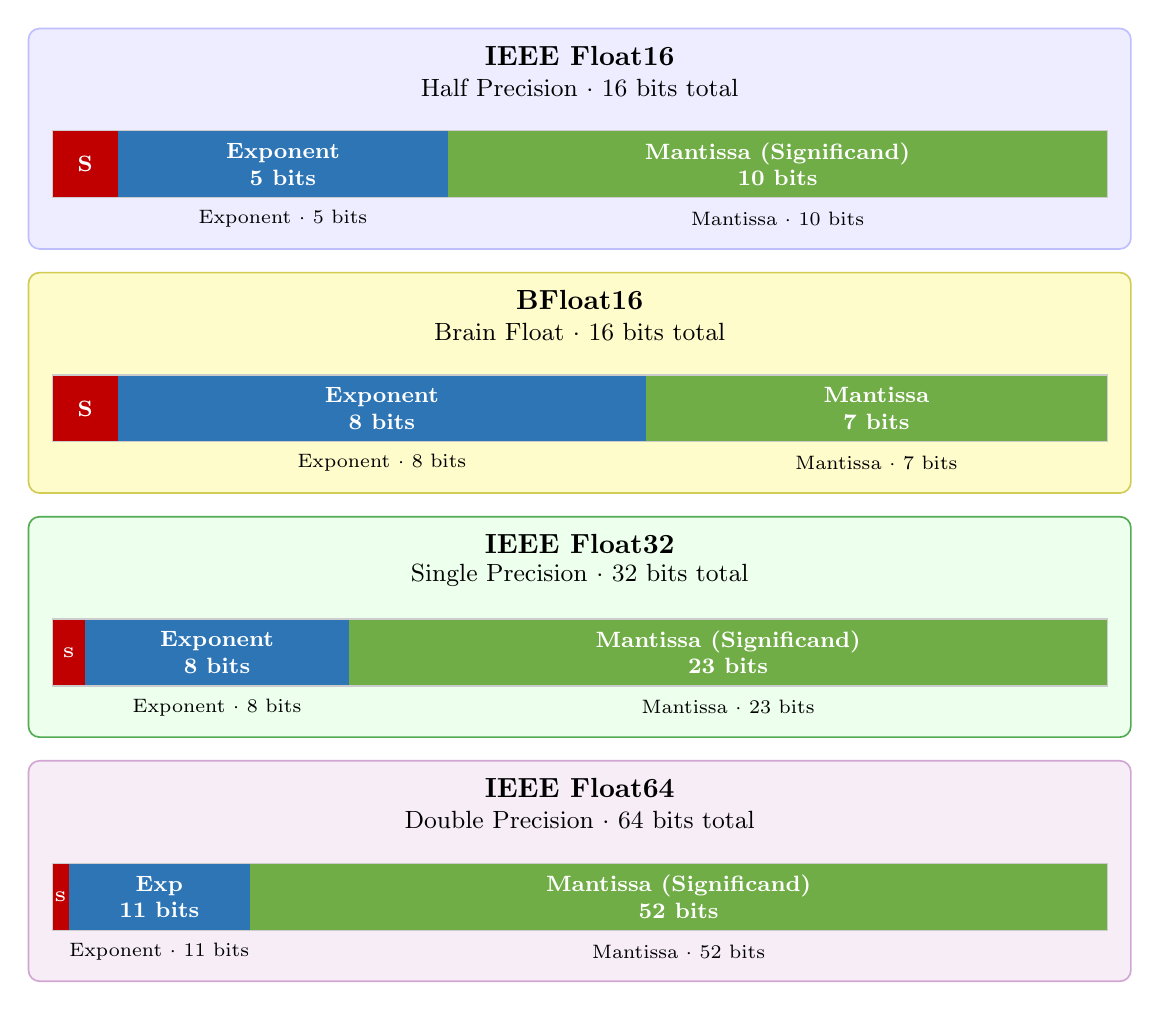
\begin{tikzpicture}[x=1cm, y=1cm]

  % ---- Color palette ----
  \definecolor{signcolor}{RGB}{192,0,0}     % red   -- sign bit
  \definecolor{expcolor} {RGB}{46,117,182}  % blue  -- exponent
  \definecolor{mancolor} {RGB}{112,173,71}  % green -- mantissa

  % ---- Panel backgrounds ----
  % Panels are 14 cm wide x 2.8 cm tall, separated by 0.3 cm gaps.
  % Y positions (bottom edge): Float16=9.30, BFloat16=6.20, Float32=3.10, Float64=0.00
  \draw[rounded corners=4pt, fill=blue!7,    draw=blue!25,        line width=0.6pt]
      (0.0,  9.30) rectangle (14.0, 12.10);  % Float16
  \draw[rounded corners=4pt, fill=yellow!20, draw=yellow!60!gray, line width=0.6pt]
      (0.0,  6.20) rectangle (14.0,  9.00);  % BFloat16
  \draw[rounded corners=4pt, fill=green!7,   draw=green!35!gray,  line width=0.6pt]
      (0.0,  3.10) rectangle (14.0,  5.90);  % Float32
  \draw[rounded corners=4pt, fill=violet!7,  draw=violet!35,      line width=0.6pt]
      (0.0,  0.00) rectangle (14.0,  2.80);  % Float64

  % ====================================================================
  % Bar geometry (shared across all panels):
  %   x range:    [0.30, 13.70]  => total bar width = 13.40 cm
  %   bar height: 0.85 cm
  %   bar bottom: panel_bottom + 0.65
  %   bar top:    panel_bottom + 1.50
  %
  % Segment x boundaries  (width = n_bits/total * 13.40):
  %   Float16  (16-bit): 0.300 | 1.138 | 5.325 | 13.700
  %   BFloat16 (16-bit): 0.300 | 1.138 | 7.838 | 13.700
  %   Float32  (32-bit): 0.300 | 0.719 | 4.069 | 13.700
  %   Float64  (64-bit): 0.300 | 0.509 | 2.813 | 13.700
  % ====================================================================

  % ------------------------------------------------------------------
  % IEEE Float16  (panel bottom y = 9.30)
  % ------------------------------------------------------------------
  \node[font=\normalsize\bfseries] at (7.0, 11.75) {IEEE Float16};
  \node[font=\small]               at (7.0, 11.35) {Half Precision $\cdot$ 16 bits total};

  % S:   1/16 * 13.40 = 0.838 cm   x: 0.300 -- 1.138,  center: 0.719
  \fill[signcolor] (0.300,  9.95) rectangle ( 1.138, 10.80);
  \node[text=white, font=\footnotesize\bfseries] at (0.719, 10.375) {S};

  % Exp: 5/16 * 13.40 = 4.188 cm   x: 1.138 -- 5.325,  center: 3.231
  \fill[expcolor]  (1.138,  9.95) rectangle ( 5.325, 10.80);
  \node[text=white, font=\footnotesize\bfseries, align=center] at (3.231, 10.375)
      {Exponent \\ 5 bits};

  % Man: 10/16 * 13.40 = 8.375 cm  x: 5.325 -- 13.700, center: 9.513
  \fill[mancolor]  (5.325,  9.95) rectangle (13.700, 10.80);
  \node[text=white, font=\footnotesize\bfseries, align=center] at (9.513, 10.375)
      {Mantissa (Significand) \\ 10 bits};

  \draw[black!20, line width=0.4pt] (0.300, 9.95) rectangle (13.700, 10.80);

  \node[font=\scriptsize] at (3.231, 9.68) {Exponent $\cdot$ 5 bits};
  \node[font=\scriptsize] at (9.513, 9.68) {Mantissa $\cdot$ 10 bits};

  % ------------------------------------------------------------------
  % BFloat16  (panel bottom y = 6.20)
  % ------------------------------------------------------------------
  \node[font=\normalsize\bfseries] at (7.0, 8.65) {BFloat16};
  \node[font=\small]               at (7.0, 8.25) {Brain Float $\cdot$ 16 bits total};

  % S:   1/16 * 13.40 = 0.838 cm   x: 0.300 -- 1.138,  center: 0.719
  \fill[signcolor] (0.300,  6.85) rectangle ( 1.138,  7.70);
  \node[text=white, font=\footnotesize\bfseries] at (0.719, 7.275) {S};

  % Exp: 8/16 * 13.40 = 6.700 cm   x: 1.138 -- 7.838,  center: 4.488
  \fill[expcolor]  (1.138,  6.85) rectangle ( 7.838,  7.70);
  \node[text=white, font=\footnotesize\bfseries, align=center] at (4.488, 7.275)
      {Exponent \\ 8 bits};

  % Man: 7/16 * 13.40 = 5.863 cm   x: 7.838 -- 13.700, center: 10.769
  \fill[mancolor]  (7.838,  6.85) rectangle (13.700,  7.70);
  \node[text=white, font=\footnotesize\bfseries, align=center] at (10.769, 7.275)
      {Mantissa \\ 7 bits};

  \draw[black!20, line width=0.4pt] (0.300, 6.85) rectangle (13.700, 7.70);

  \node[font=\scriptsize] at ( 4.488, 6.58) {Exponent $\cdot$ 8 bits};
  \node[font=\scriptsize] at (10.769, 6.58) {Mantissa $\cdot$ 7 bits};

  % ------------------------------------------------------------------
  % IEEE Float32  (panel bottom y = 3.10)
  % ------------------------------------------------------------------
  \node[font=\normalsize\bfseries] at (7.0, 5.55) {IEEE Float32};
  \node[font=\small]               at (7.0, 5.15) {Single Precision $\cdot$ 32 bits total};

  % S:   1/32 * 13.40 = 0.419 cm   x: 0.300 -- 0.719,  center: 0.510
  \fill[signcolor] (0.300,  3.75) rectangle ( 0.719,  4.60);
  \node[text=white, font=\tiny\bfseries] at (0.510, 4.175) {S};

  % Exp: 8/32 * 13.40 = 3.350 cm   x: 0.719 -- 4.069,  center: 2.394
  \fill[expcolor]  (0.719,  3.75) rectangle ( 4.069,  4.60);
  \node[text=white, font=\footnotesize\bfseries, align=center] at (2.394, 4.175)
      {Exponent \\ 8 bits};

  % Man: 23/32 * 13.40 = 9.631 cm  x: 4.069 -- 13.700, center: 8.885
  \fill[mancolor]  (4.069,  3.75) rectangle (13.700,  4.60);
  \node[text=white, font=\footnotesize\bfseries, align=center] at (8.885, 4.175)
      {Mantissa (Significand) \\ 23 bits};

  \draw[black!20, line width=0.4pt] (0.300, 3.75) rectangle (13.700, 4.60);

  \node[font=\scriptsize] at (2.394, 3.48) {Exponent $\cdot$ 8 bits};
  \node[font=\scriptsize] at (8.885, 3.48) {Mantissa $\cdot$ 23 bits};

  % ------------------------------------------------------------------
  % IEEE Float64  (panel bottom y = 0.00)
  % ------------------------------------------------------------------
  \node[font=\normalsize\bfseries] at (7.0, 2.45) {IEEE Float64};
  \node[font=\small]               at (7.0, 2.05) {Double Precision $\cdot$ 64 bits total};

  % S:    1/64 * 13.40 = 0.209 cm  x: 0.300 -- 0.509,  center: 0.405
  \fill[signcolor] (0.300,  0.65) rectangle ( 0.509,  1.50);
  \node[text=white, font=\tiny\bfseries] at (0.405, 1.075) {S};

  % Exp: 11/64 * 13.40 = 2.303 cm  x: 0.509 -- 2.813,  center: 1.661
  \fill[expcolor]  (0.509,  0.65) rectangle ( 2.813,  1.50);
  \node[text=white, font=\footnotesize\bfseries, align=center] at (1.661, 1.075)
      {Exp \\ 11 bits};

  % Man: 52/64 * 13.40 = 10.888 cm x: 2.813 -- 13.700, center: 8.257
  \fill[mancolor]  (2.813,  0.65) rectangle (13.700,  1.50);
  \node[text=white, font=\footnotesize\bfseries, align=center] at (8.257, 1.075)
      {Mantissa (Significand) \\ 52 bits};

  \draw[black!20, line width=0.4pt] (0.300, 0.65) rectangle (13.700, 1.50);

  \node[font=\scriptsize] at (1.661, 0.38) {Exponent $\cdot$ 11 bits};
  \node[font=\scriptsize] at (8.257, 0.38) {Mantissa $\cdot$ 52 bits};

\end{tikzpicture}
}
%     \caption{...}
%     \label{fig:float-formats}
%   \end{figure}
% --------------------------------------------------------------------
%
% Layout: 4 panels stacked vertically, each 14 cm x 2.8 cm.
% Bar widths are proportional to actual bit-field widths.
%   Float16:  S=1, Exp=5,  Man=10  (16 bits total)
%   BFloat16: S=1, Exp=8,  Man=7   (16 bits total)
%   Float32:  S=1, Exp=8,  Man=23  (32 bits total)
%   Float64:  S=1, Exp=11, Man=52  (64 bits total)

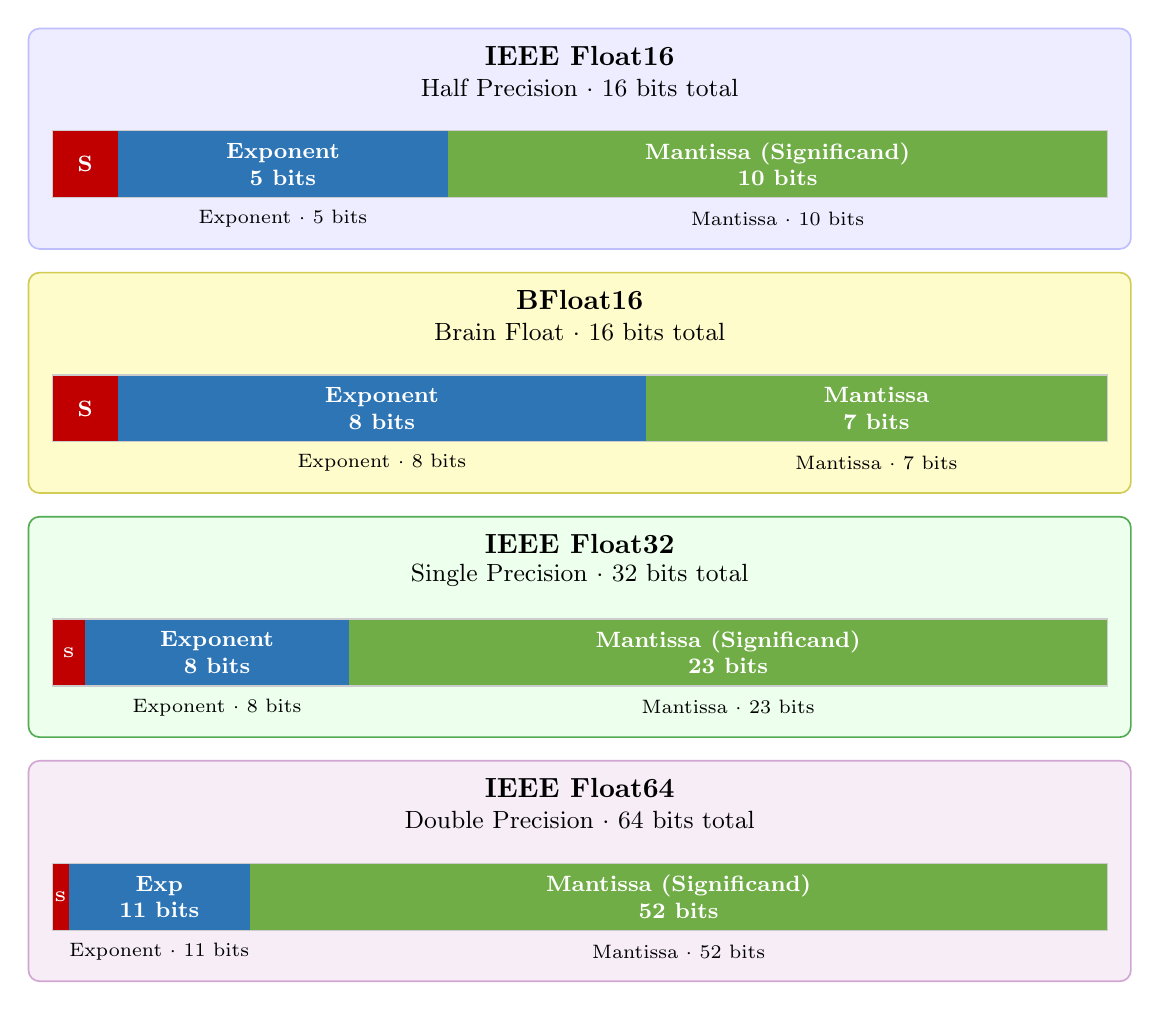
\begin{tikzpicture}[x=1cm, y=1cm]

  % ---- Color palette ----
  \definecolor{signcolor}{RGB}{192,0,0}     % red   -- sign bit
  \definecolor{expcolor} {RGB}{46,117,182}  % blue  -- exponent
  \definecolor{mancolor} {RGB}{112,173,71}  % green -- mantissa

  % ---- Panel backgrounds ----
  % Panels are 14 cm wide x 2.8 cm tall, separated by 0.3 cm gaps.
  % Y positions (bottom edge): Float16=9.30, BFloat16=6.20, Float32=3.10, Float64=0.00
  \draw[rounded corners=4pt, fill=blue!7,    draw=blue!25,        line width=0.6pt]
      (0.0,  9.30) rectangle (14.0, 12.10);  % Float16
  \draw[rounded corners=4pt, fill=yellow!20, draw=yellow!60!gray, line width=0.6pt]
      (0.0,  6.20) rectangle (14.0,  9.00);  % BFloat16
  \draw[rounded corners=4pt, fill=green!7,   draw=green!35!gray,  line width=0.6pt]
      (0.0,  3.10) rectangle (14.0,  5.90);  % Float32
  \draw[rounded corners=4pt, fill=violet!7,  draw=violet!35,      line width=0.6pt]
      (0.0,  0.00) rectangle (14.0,  2.80);  % Float64

  % ====================================================================
  % Bar geometry (shared across all panels):
  %   x range:    [0.30, 13.70]  => total bar width = 13.40 cm
  %   bar height: 0.85 cm
  %   bar bottom: panel_bottom + 0.65
  %   bar top:    panel_bottom + 1.50
  %
  % Segment x boundaries  (width = n_bits/total * 13.40):
  %   Float16  (16-bit): 0.300 | 1.138 | 5.325 | 13.700
  %   BFloat16 (16-bit): 0.300 | 1.138 | 7.838 | 13.700
  %   Float32  (32-bit): 0.300 | 0.719 | 4.069 | 13.700
  %   Float64  (64-bit): 0.300 | 0.509 | 2.813 | 13.700
  % ====================================================================

  % ------------------------------------------------------------------
  % IEEE Float16  (panel bottom y = 9.30)
  % ------------------------------------------------------------------
  \node[font=\normalsize\bfseries] at (7.0, 11.75) {IEEE Float16};
  \node[font=\small]               at (7.0, 11.35) {Half Precision $\cdot$ 16 bits total};

  % S:   1/16 * 13.40 = 0.838 cm   x: 0.300 -- 1.138,  center: 0.719
  \fill[signcolor] (0.300,  9.95) rectangle ( 1.138, 10.80);
  \node[text=white, font=\footnotesize\bfseries] at (0.719, 10.375) {S};

  % Exp: 5/16 * 13.40 = 4.188 cm   x: 1.138 -- 5.325,  center: 3.231
  \fill[expcolor]  (1.138,  9.95) rectangle ( 5.325, 10.80);
  \node[text=white, font=\footnotesize\bfseries, align=center] at (3.231, 10.375)
      {Exponent \\ 5 bits};

  % Man: 10/16 * 13.40 = 8.375 cm  x: 5.325 -- 13.700, center: 9.513
  \fill[mancolor]  (5.325,  9.95) rectangle (13.700, 10.80);
  \node[text=white, font=\footnotesize\bfseries, align=center] at (9.513, 10.375)
      {Mantissa (Significand) \\ 10 bits};

  \draw[black!20, line width=0.4pt] (0.300, 9.95) rectangle (13.700, 10.80);

  \node[font=\scriptsize] at (3.231, 9.68) {Exponent $\cdot$ 5 bits};
  \node[font=\scriptsize] at (9.513, 9.68) {Mantissa $\cdot$ 10 bits};

  % ------------------------------------------------------------------
  % BFloat16  (panel bottom y = 6.20)
  % ------------------------------------------------------------------
  \node[font=\normalsize\bfseries] at (7.0, 8.65) {BFloat16};
  \node[font=\small]               at (7.0, 8.25) {Brain Float $\cdot$ 16 bits total};

  % S:   1/16 * 13.40 = 0.838 cm   x: 0.300 -- 1.138,  center: 0.719
  \fill[signcolor] (0.300,  6.85) rectangle ( 1.138,  7.70);
  \node[text=white, font=\footnotesize\bfseries] at (0.719, 7.275) {S};

  % Exp: 8/16 * 13.40 = 6.700 cm   x: 1.138 -- 7.838,  center: 4.488
  \fill[expcolor]  (1.138,  6.85) rectangle ( 7.838,  7.70);
  \node[text=white, font=\footnotesize\bfseries, align=center] at (4.488, 7.275)
      {Exponent \\ 8 bits};

  % Man: 7/16 * 13.40 = 5.863 cm   x: 7.838 -- 13.700, center: 10.769
  \fill[mancolor]  (7.838,  6.85) rectangle (13.700,  7.70);
  \node[text=white, font=\footnotesize\bfseries, align=center] at (10.769, 7.275)
      {Mantissa \\ 7 bits};

  \draw[black!20, line width=0.4pt] (0.300, 6.85) rectangle (13.700, 7.70);

  \node[font=\scriptsize] at ( 4.488, 6.58) {Exponent $\cdot$ 8 bits};
  \node[font=\scriptsize] at (10.769, 6.58) {Mantissa $\cdot$ 7 bits};

  % ------------------------------------------------------------------
  % IEEE Float32  (panel bottom y = 3.10)
  % ------------------------------------------------------------------
  \node[font=\normalsize\bfseries] at (7.0, 5.55) {IEEE Float32};
  \node[font=\small]               at (7.0, 5.15) {Single Precision $\cdot$ 32 bits total};

  % S:   1/32 * 13.40 = 0.419 cm   x: 0.300 -- 0.719,  center: 0.510
  \fill[signcolor] (0.300,  3.75) rectangle ( 0.719,  4.60);
  \node[text=white, font=\tiny\bfseries] at (0.510, 4.175) {S};

  % Exp: 8/32 * 13.40 = 3.350 cm   x: 0.719 -- 4.069,  center: 2.394
  \fill[expcolor]  (0.719,  3.75) rectangle ( 4.069,  4.60);
  \node[text=white, font=\footnotesize\bfseries, align=center] at (2.394, 4.175)
      {Exponent \\ 8 bits};

  % Man: 23/32 * 13.40 = 9.631 cm  x: 4.069 -- 13.700, center: 8.885
  \fill[mancolor]  (4.069,  3.75) rectangle (13.700,  4.60);
  \node[text=white, font=\footnotesize\bfseries, align=center] at (8.885, 4.175)
      {Mantissa (Significand) \\ 23 bits};

  \draw[black!20, line width=0.4pt] (0.300, 3.75) rectangle (13.700, 4.60);

  \node[font=\scriptsize] at (2.394, 3.48) {Exponent $\cdot$ 8 bits};
  \node[font=\scriptsize] at (8.885, 3.48) {Mantissa $\cdot$ 23 bits};

  % ------------------------------------------------------------------
  % IEEE Float64  (panel bottom y = 0.00)
  % ------------------------------------------------------------------
  \node[font=\normalsize\bfseries] at (7.0, 2.45) {IEEE Float64};
  \node[font=\small]               at (7.0, 2.05) {Double Precision $\cdot$ 64 bits total};

  % S:    1/64 * 13.40 = 0.209 cm  x: 0.300 -- 0.509,  center: 0.405
  \fill[signcolor] (0.300,  0.65) rectangle ( 0.509,  1.50);
  \node[text=white, font=\tiny\bfseries] at (0.405, 1.075) {S};

  % Exp: 11/64 * 13.40 = 2.303 cm  x: 0.509 -- 2.813,  center: 1.661
  \fill[expcolor]  (0.509,  0.65) rectangle ( 2.813,  1.50);
  \node[text=white, font=\footnotesize\bfseries, align=center] at (1.661, 1.075)
      {Exp \\ 11 bits};

  % Man: 52/64 * 13.40 = 10.888 cm x: 2.813 -- 13.700, center: 8.257
  \fill[mancolor]  (2.813,  0.65) rectangle (13.700,  1.50);
  \node[text=white, font=\footnotesize\bfseries, align=center] at (8.257, 1.075)
      {Mantissa (Significand) \\ 52 bits};

  \draw[black!20, line width=0.4pt] (0.300, 0.65) rectangle (13.700, 1.50);

  \node[font=\scriptsize] at (1.661, 0.38) {Exponent $\cdot$ 11 bits};
  \node[font=\scriptsize] at (8.257, 0.38) {Mantissa $\cdot$ 52 bits};

\end{tikzpicture}
}
%
%   Fit to the full page width (~17.8 cm in IEEE two-column):
%     \resizebox{\textwidth}{!}{% Floating-point format comparison — single-column stack layout
%
% Required in preamble:
%   \usepackage{tikz}
%
% ---- Scaling -------------------------------------------------------
% The tikzpicture is drawn at its natural size: 14 cm wide x 12.1 cm tall.
% Use \resizebox (from the graphicx package, always loaded in IEEE style)
% to scale it to whatever width you need. The height adjusts automatically.
%
%   Fit to a single text column (~8.8 cm in IEEE two-column):
%     \resizebox{\columnwidth}{!}{% Floating-point format comparison — single-column stack layout
%
% Required in preamble:
%   \usepackage{tikz}
%
% ---- Scaling -------------------------------------------------------
% The tikzpicture is drawn at its natural size: 14 cm wide x 12.1 cm tall.
% Use \resizebox (from the graphicx package, always loaded in IEEE style)
% to scale it to whatever width you need. The height adjusts automatically.
%
%   Fit to a single text column (~8.8 cm in IEEE two-column):
%     \resizebox{\columnwidth}{!}{\input{float_formats_tikz.tex}}
%
%   Fit to the full page width (~17.8 cm in IEEE two-column):
%     \resizebox{\textwidth}{!}{\input{float_formats_tikz.tex}}
%
%   Fit to an arbitrary fraction of the column width:
%     \resizebox{0.9\columnwidth}{!}{\input{float_formats_tikz.tex}}
%
% \resizebox scales everything uniformly — coordinates, line widths,
% and fonts — so the result looks identical regardless of the chosen width.
%
% Recommended figure wrapper (single column):
%   \begin{figure}[t]
%     \centering
%     \resizebox{\columnwidth}{!}{\input{float_formats_tikz.tex}}
%     \caption{...}
%     \label{fig:float-formats}
%   \end{figure}
% --------------------------------------------------------------------
%
% Layout: 4 panels stacked vertically, each 14 cm x 2.8 cm.
% Bar widths are proportional to actual bit-field widths.
%   Float16:  S=1, Exp=5,  Man=10  (16 bits total)
%   BFloat16: S=1, Exp=8,  Man=7   (16 bits total)
%   Float32:  S=1, Exp=8,  Man=23  (32 bits total)
%   Float64:  S=1, Exp=11, Man=52  (64 bits total)

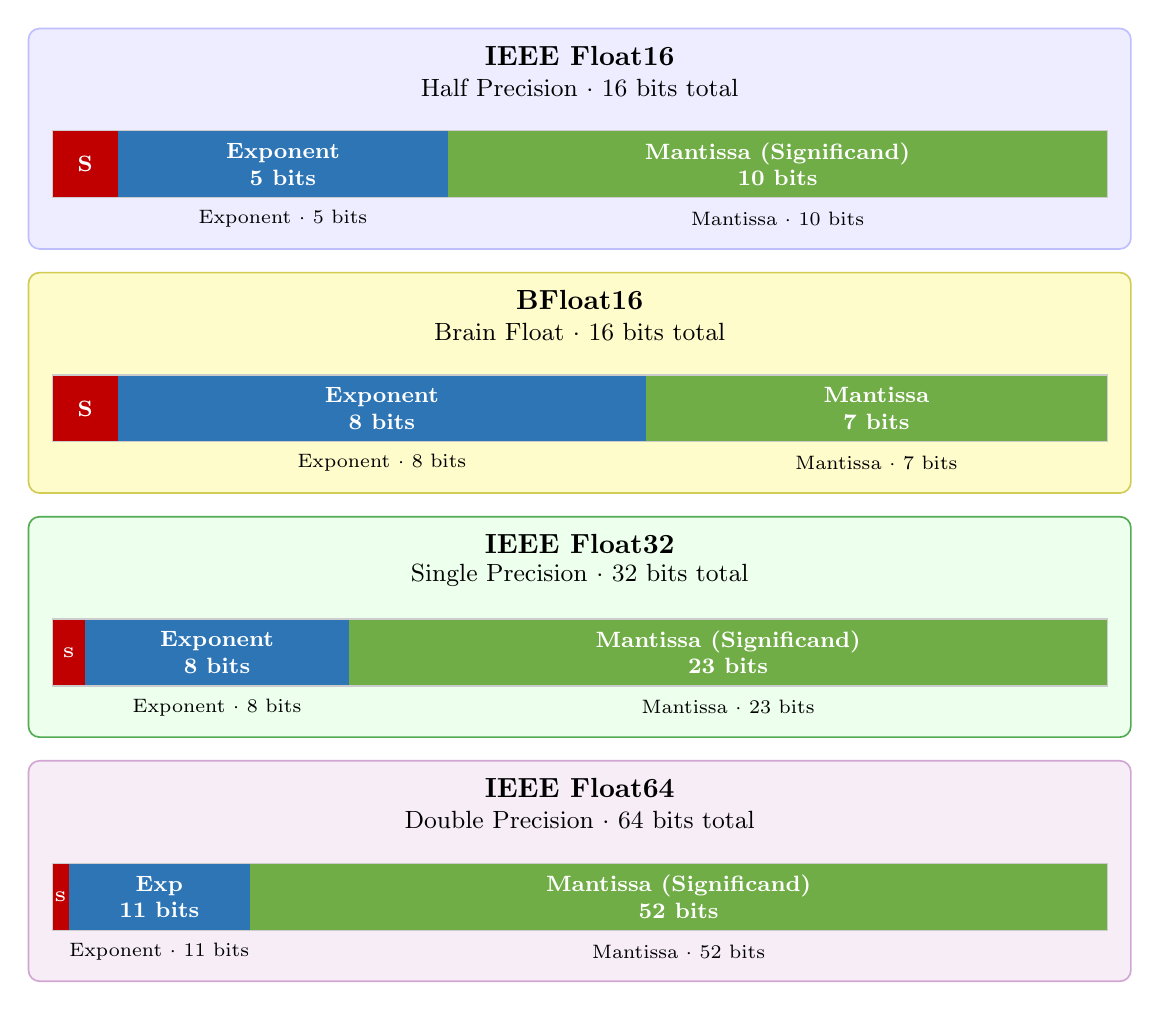
\begin{tikzpicture}[x=1cm, y=1cm]

  % ---- Color palette ----
  \definecolor{signcolor}{RGB}{192,0,0}     % red   -- sign bit
  \definecolor{expcolor} {RGB}{46,117,182}  % blue  -- exponent
  \definecolor{mancolor} {RGB}{112,173,71}  % green -- mantissa

  % ---- Panel backgrounds ----
  % Panels are 14 cm wide x 2.8 cm tall, separated by 0.3 cm gaps.
  % Y positions (bottom edge): Float16=9.30, BFloat16=6.20, Float32=3.10, Float64=0.00
  \draw[rounded corners=4pt, fill=blue!7,    draw=blue!25,        line width=0.6pt]
      (0.0,  9.30) rectangle (14.0, 12.10);  % Float16
  \draw[rounded corners=4pt, fill=yellow!20, draw=yellow!60!gray, line width=0.6pt]
      (0.0,  6.20) rectangle (14.0,  9.00);  % BFloat16
  \draw[rounded corners=4pt, fill=green!7,   draw=green!35!gray,  line width=0.6pt]
      (0.0,  3.10) rectangle (14.0,  5.90);  % Float32
  \draw[rounded corners=4pt, fill=violet!7,  draw=violet!35,      line width=0.6pt]
      (0.0,  0.00) rectangle (14.0,  2.80);  % Float64

  % ====================================================================
  % Bar geometry (shared across all panels):
  %   x range:    [0.30, 13.70]  => total bar width = 13.40 cm
  %   bar height: 0.85 cm
  %   bar bottom: panel_bottom + 0.65
  %   bar top:    panel_bottom + 1.50
  %
  % Segment x boundaries  (width = n_bits/total * 13.40):
  %   Float16  (16-bit): 0.300 | 1.138 | 5.325 | 13.700
  %   BFloat16 (16-bit): 0.300 | 1.138 | 7.838 | 13.700
  %   Float32  (32-bit): 0.300 | 0.719 | 4.069 | 13.700
  %   Float64  (64-bit): 0.300 | 0.509 | 2.813 | 13.700
  % ====================================================================

  % ------------------------------------------------------------------
  % IEEE Float16  (panel bottom y = 9.30)
  % ------------------------------------------------------------------
  \node[font=\normalsize\bfseries] at (7.0, 11.75) {IEEE Float16};
  \node[font=\small]               at (7.0, 11.35) {Half Precision $\cdot$ 16 bits total};

  % S:   1/16 * 13.40 = 0.838 cm   x: 0.300 -- 1.138,  center: 0.719
  \fill[signcolor] (0.300,  9.95) rectangle ( 1.138, 10.80);
  \node[text=white, font=\footnotesize\bfseries] at (0.719, 10.375) {S};

  % Exp: 5/16 * 13.40 = 4.188 cm   x: 1.138 -- 5.325,  center: 3.231
  \fill[expcolor]  (1.138,  9.95) rectangle ( 5.325, 10.80);
  \node[text=white, font=\footnotesize\bfseries, align=center] at (3.231, 10.375)
      {Exponent \\ 5 bits};

  % Man: 10/16 * 13.40 = 8.375 cm  x: 5.325 -- 13.700, center: 9.513
  \fill[mancolor]  (5.325,  9.95) rectangle (13.700, 10.80);
  \node[text=white, font=\footnotesize\bfseries, align=center] at (9.513, 10.375)
      {Mantissa (Significand) \\ 10 bits};

  \draw[black!20, line width=0.4pt] (0.300, 9.95) rectangle (13.700, 10.80);

  \node[font=\scriptsize] at (3.231, 9.68) {Exponent $\cdot$ 5 bits};
  \node[font=\scriptsize] at (9.513, 9.68) {Mantissa $\cdot$ 10 bits};

  % ------------------------------------------------------------------
  % BFloat16  (panel bottom y = 6.20)
  % ------------------------------------------------------------------
  \node[font=\normalsize\bfseries] at (7.0, 8.65) {BFloat16};
  \node[font=\small]               at (7.0, 8.25) {Brain Float $\cdot$ 16 bits total};

  % S:   1/16 * 13.40 = 0.838 cm   x: 0.300 -- 1.138,  center: 0.719
  \fill[signcolor] (0.300,  6.85) rectangle ( 1.138,  7.70);
  \node[text=white, font=\footnotesize\bfseries] at (0.719, 7.275) {S};

  % Exp: 8/16 * 13.40 = 6.700 cm   x: 1.138 -- 7.838,  center: 4.488
  \fill[expcolor]  (1.138,  6.85) rectangle ( 7.838,  7.70);
  \node[text=white, font=\footnotesize\bfseries, align=center] at (4.488, 7.275)
      {Exponent \\ 8 bits};

  % Man: 7/16 * 13.40 = 5.863 cm   x: 7.838 -- 13.700, center: 10.769
  \fill[mancolor]  (7.838,  6.85) rectangle (13.700,  7.70);
  \node[text=white, font=\footnotesize\bfseries, align=center] at (10.769, 7.275)
      {Mantissa \\ 7 bits};

  \draw[black!20, line width=0.4pt] (0.300, 6.85) rectangle (13.700, 7.70);

  \node[font=\scriptsize] at ( 4.488, 6.58) {Exponent $\cdot$ 8 bits};
  \node[font=\scriptsize] at (10.769, 6.58) {Mantissa $\cdot$ 7 bits};

  % ------------------------------------------------------------------
  % IEEE Float32  (panel bottom y = 3.10)
  % ------------------------------------------------------------------
  \node[font=\normalsize\bfseries] at (7.0, 5.55) {IEEE Float32};
  \node[font=\small]               at (7.0, 5.15) {Single Precision $\cdot$ 32 bits total};

  % S:   1/32 * 13.40 = 0.419 cm   x: 0.300 -- 0.719,  center: 0.510
  \fill[signcolor] (0.300,  3.75) rectangle ( 0.719,  4.60);
  \node[text=white, font=\tiny\bfseries] at (0.510, 4.175) {S};

  % Exp: 8/32 * 13.40 = 3.350 cm   x: 0.719 -- 4.069,  center: 2.394
  \fill[expcolor]  (0.719,  3.75) rectangle ( 4.069,  4.60);
  \node[text=white, font=\footnotesize\bfseries, align=center] at (2.394, 4.175)
      {Exponent \\ 8 bits};

  % Man: 23/32 * 13.40 = 9.631 cm  x: 4.069 -- 13.700, center: 8.885
  \fill[mancolor]  (4.069,  3.75) rectangle (13.700,  4.60);
  \node[text=white, font=\footnotesize\bfseries, align=center] at (8.885, 4.175)
      {Mantissa (Significand) \\ 23 bits};

  \draw[black!20, line width=0.4pt] (0.300, 3.75) rectangle (13.700, 4.60);

  \node[font=\scriptsize] at (2.394, 3.48) {Exponent $\cdot$ 8 bits};
  \node[font=\scriptsize] at (8.885, 3.48) {Mantissa $\cdot$ 23 bits};

  % ------------------------------------------------------------------
  % IEEE Float64  (panel bottom y = 0.00)
  % ------------------------------------------------------------------
  \node[font=\normalsize\bfseries] at (7.0, 2.45) {IEEE Float64};
  \node[font=\small]               at (7.0, 2.05) {Double Precision $\cdot$ 64 bits total};

  % S:    1/64 * 13.40 = 0.209 cm  x: 0.300 -- 0.509,  center: 0.405
  \fill[signcolor] (0.300,  0.65) rectangle ( 0.509,  1.50);
  \node[text=white, font=\tiny\bfseries] at (0.405, 1.075) {S};

  % Exp: 11/64 * 13.40 = 2.303 cm  x: 0.509 -- 2.813,  center: 1.661
  \fill[expcolor]  (0.509,  0.65) rectangle ( 2.813,  1.50);
  \node[text=white, font=\footnotesize\bfseries, align=center] at (1.661, 1.075)
      {Exp \\ 11 bits};

  % Man: 52/64 * 13.40 = 10.888 cm x: 2.813 -- 13.700, center: 8.257
  \fill[mancolor]  (2.813,  0.65) rectangle (13.700,  1.50);
  \node[text=white, font=\footnotesize\bfseries, align=center] at (8.257, 1.075)
      {Mantissa (Significand) \\ 52 bits};

  \draw[black!20, line width=0.4pt] (0.300, 0.65) rectangle (13.700, 1.50);

  \node[font=\scriptsize] at (1.661, 0.38) {Exponent $\cdot$ 11 bits};
  \node[font=\scriptsize] at (8.257, 0.38) {Mantissa $\cdot$ 52 bits};

\end{tikzpicture}
}
%
%   Fit to the full page width (~17.8 cm in IEEE two-column):
%     \resizebox{\textwidth}{!}{% Floating-point format comparison — single-column stack layout
%
% Required in preamble:
%   \usepackage{tikz}
%
% ---- Scaling -------------------------------------------------------
% The tikzpicture is drawn at its natural size: 14 cm wide x 12.1 cm tall.
% Use \resizebox (from the graphicx package, always loaded in IEEE style)
% to scale it to whatever width you need. The height adjusts automatically.
%
%   Fit to a single text column (~8.8 cm in IEEE two-column):
%     \resizebox{\columnwidth}{!}{\input{float_formats_tikz.tex}}
%
%   Fit to the full page width (~17.8 cm in IEEE two-column):
%     \resizebox{\textwidth}{!}{\input{float_formats_tikz.tex}}
%
%   Fit to an arbitrary fraction of the column width:
%     \resizebox{0.9\columnwidth}{!}{\input{float_formats_tikz.tex}}
%
% \resizebox scales everything uniformly — coordinates, line widths,
% and fonts — so the result looks identical regardless of the chosen width.
%
% Recommended figure wrapper (single column):
%   \begin{figure}[t]
%     \centering
%     \resizebox{\columnwidth}{!}{\input{float_formats_tikz.tex}}
%     \caption{...}
%     \label{fig:float-formats}
%   \end{figure}
% --------------------------------------------------------------------
%
% Layout: 4 panels stacked vertically, each 14 cm x 2.8 cm.
% Bar widths are proportional to actual bit-field widths.
%   Float16:  S=1, Exp=5,  Man=10  (16 bits total)
%   BFloat16: S=1, Exp=8,  Man=7   (16 bits total)
%   Float32:  S=1, Exp=8,  Man=23  (32 bits total)
%   Float64:  S=1, Exp=11, Man=52  (64 bits total)

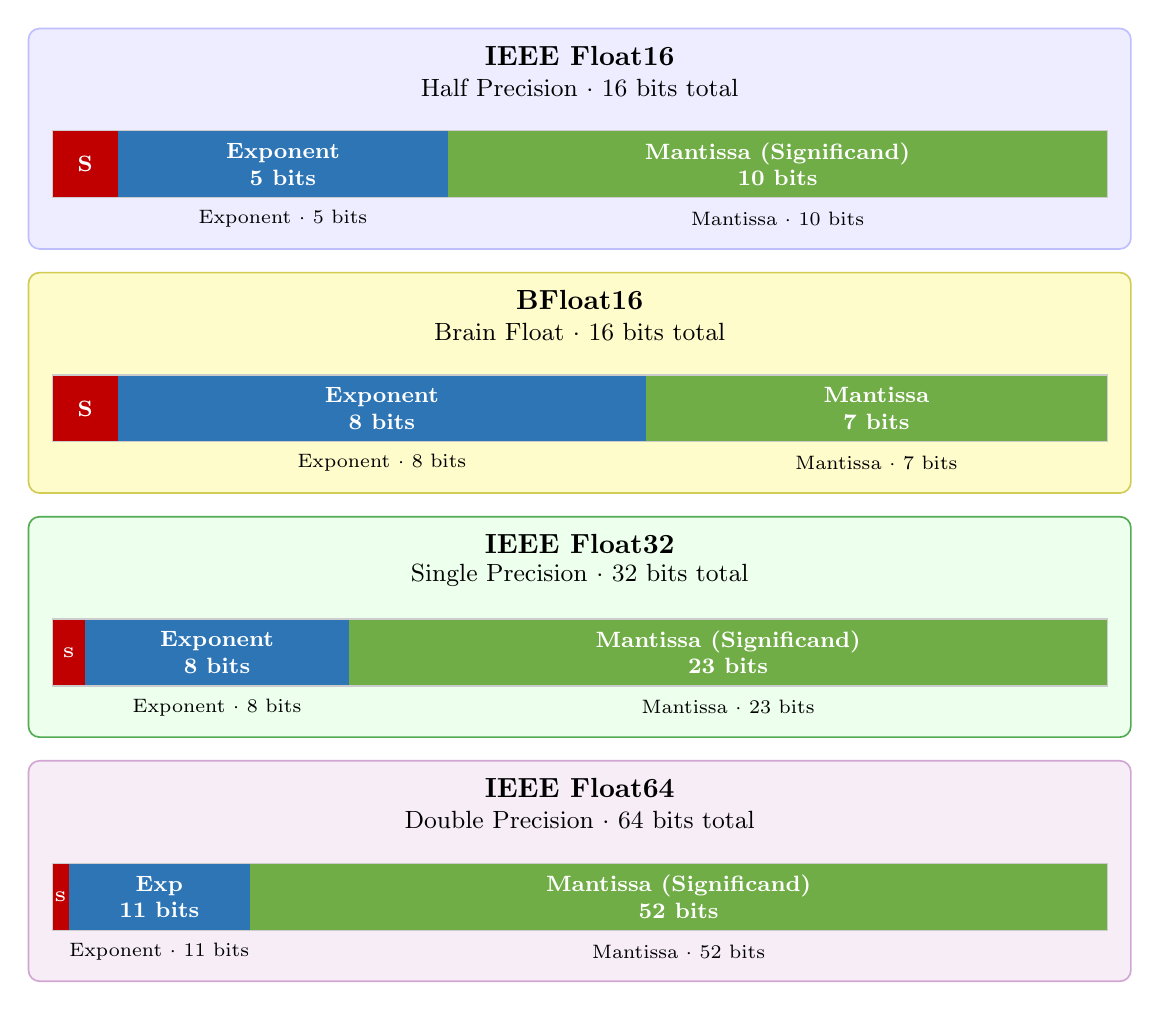
\begin{tikzpicture}[x=1cm, y=1cm]

  % ---- Color palette ----
  \definecolor{signcolor}{RGB}{192,0,0}     % red   -- sign bit
  \definecolor{expcolor} {RGB}{46,117,182}  % blue  -- exponent
  \definecolor{mancolor} {RGB}{112,173,71}  % green -- mantissa

  % ---- Panel backgrounds ----
  % Panels are 14 cm wide x 2.8 cm tall, separated by 0.3 cm gaps.
  % Y positions (bottom edge): Float16=9.30, BFloat16=6.20, Float32=3.10, Float64=0.00
  \draw[rounded corners=4pt, fill=blue!7,    draw=blue!25,        line width=0.6pt]
      (0.0,  9.30) rectangle (14.0, 12.10);  % Float16
  \draw[rounded corners=4pt, fill=yellow!20, draw=yellow!60!gray, line width=0.6pt]
      (0.0,  6.20) rectangle (14.0,  9.00);  % BFloat16
  \draw[rounded corners=4pt, fill=green!7,   draw=green!35!gray,  line width=0.6pt]
      (0.0,  3.10) rectangle (14.0,  5.90);  % Float32
  \draw[rounded corners=4pt, fill=violet!7,  draw=violet!35,      line width=0.6pt]
      (0.0,  0.00) rectangle (14.0,  2.80);  % Float64

  % ====================================================================
  % Bar geometry (shared across all panels):
  %   x range:    [0.30, 13.70]  => total bar width = 13.40 cm
  %   bar height: 0.85 cm
  %   bar bottom: panel_bottom + 0.65
  %   bar top:    panel_bottom + 1.50
  %
  % Segment x boundaries  (width = n_bits/total * 13.40):
  %   Float16  (16-bit): 0.300 | 1.138 | 5.325 | 13.700
  %   BFloat16 (16-bit): 0.300 | 1.138 | 7.838 | 13.700
  %   Float32  (32-bit): 0.300 | 0.719 | 4.069 | 13.700
  %   Float64  (64-bit): 0.300 | 0.509 | 2.813 | 13.700
  % ====================================================================

  % ------------------------------------------------------------------
  % IEEE Float16  (panel bottom y = 9.30)
  % ------------------------------------------------------------------
  \node[font=\normalsize\bfseries] at (7.0, 11.75) {IEEE Float16};
  \node[font=\small]               at (7.0, 11.35) {Half Precision $\cdot$ 16 bits total};

  % S:   1/16 * 13.40 = 0.838 cm   x: 0.300 -- 1.138,  center: 0.719
  \fill[signcolor] (0.300,  9.95) rectangle ( 1.138, 10.80);
  \node[text=white, font=\footnotesize\bfseries] at (0.719, 10.375) {S};

  % Exp: 5/16 * 13.40 = 4.188 cm   x: 1.138 -- 5.325,  center: 3.231
  \fill[expcolor]  (1.138,  9.95) rectangle ( 5.325, 10.80);
  \node[text=white, font=\footnotesize\bfseries, align=center] at (3.231, 10.375)
      {Exponent \\ 5 bits};

  % Man: 10/16 * 13.40 = 8.375 cm  x: 5.325 -- 13.700, center: 9.513
  \fill[mancolor]  (5.325,  9.95) rectangle (13.700, 10.80);
  \node[text=white, font=\footnotesize\bfseries, align=center] at (9.513, 10.375)
      {Mantissa (Significand) \\ 10 bits};

  \draw[black!20, line width=0.4pt] (0.300, 9.95) rectangle (13.700, 10.80);

  \node[font=\scriptsize] at (3.231, 9.68) {Exponent $\cdot$ 5 bits};
  \node[font=\scriptsize] at (9.513, 9.68) {Mantissa $\cdot$ 10 bits};

  % ------------------------------------------------------------------
  % BFloat16  (panel bottom y = 6.20)
  % ------------------------------------------------------------------
  \node[font=\normalsize\bfseries] at (7.0, 8.65) {BFloat16};
  \node[font=\small]               at (7.0, 8.25) {Brain Float $\cdot$ 16 bits total};

  % S:   1/16 * 13.40 = 0.838 cm   x: 0.300 -- 1.138,  center: 0.719
  \fill[signcolor] (0.300,  6.85) rectangle ( 1.138,  7.70);
  \node[text=white, font=\footnotesize\bfseries] at (0.719, 7.275) {S};

  % Exp: 8/16 * 13.40 = 6.700 cm   x: 1.138 -- 7.838,  center: 4.488
  \fill[expcolor]  (1.138,  6.85) rectangle ( 7.838,  7.70);
  \node[text=white, font=\footnotesize\bfseries, align=center] at (4.488, 7.275)
      {Exponent \\ 8 bits};

  % Man: 7/16 * 13.40 = 5.863 cm   x: 7.838 -- 13.700, center: 10.769
  \fill[mancolor]  (7.838,  6.85) rectangle (13.700,  7.70);
  \node[text=white, font=\footnotesize\bfseries, align=center] at (10.769, 7.275)
      {Mantissa \\ 7 bits};

  \draw[black!20, line width=0.4pt] (0.300, 6.85) rectangle (13.700, 7.70);

  \node[font=\scriptsize] at ( 4.488, 6.58) {Exponent $\cdot$ 8 bits};
  \node[font=\scriptsize] at (10.769, 6.58) {Mantissa $\cdot$ 7 bits};

  % ------------------------------------------------------------------
  % IEEE Float32  (panel bottom y = 3.10)
  % ------------------------------------------------------------------
  \node[font=\normalsize\bfseries] at (7.0, 5.55) {IEEE Float32};
  \node[font=\small]               at (7.0, 5.15) {Single Precision $\cdot$ 32 bits total};

  % S:   1/32 * 13.40 = 0.419 cm   x: 0.300 -- 0.719,  center: 0.510
  \fill[signcolor] (0.300,  3.75) rectangle ( 0.719,  4.60);
  \node[text=white, font=\tiny\bfseries] at (0.510, 4.175) {S};

  % Exp: 8/32 * 13.40 = 3.350 cm   x: 0.719 -- 4.069,  center: 2.394
  \fill[expcolor]  (0.719,  3.75) rectangle ( 4.069,  4.60);
  \node[text=white, font=\footnotesize\bfseries, align=center] at (2.394, 4.175)
      {Exponent \\ 8 bits};

  % Man: 23/32 * 13.40 = 9.631 cm  x: 4.069 -- 13.700, center: 8.885
  \fill[mancolor]  (4.069,  3.75) rectangle (13.700,  4.60);
  \node[text=white, font=\footnotesize\bfseries, align=center] at (8.885, 4.175)
      {Mantissa (Significand) \\ 23 bits};

  \draw[black!20, line width=0.4pt] (0.300, 3.75) rectangle (13.700, 4.60);

  \node[font=\scriptsize] at (2.394, 3.48) {Exponent $\cdot$ 8 bits};
  \node[font=\scriptsize] at (8.885, 3.48) {Mantissa $\cdot$ 23 bits};

  % ------------------------------------------------------------------
  % IEEE Float64  (panel bottom y = 0.00)
  % ------------------------------------------------------------------
  \node[font=\normalsize\bfseries] at (7.0, 2.45) {IEEE Float64};
  \node[font=\small]               at (7.0, 2.05) {Double Precision $\cdot$ 64 bits total};

  % S:    1/64 * 13.40 = 0.209 cm  x: 0.300 -- 0.509,  center: 0.405
  \fill[signcolor] (0.300,  0.65) rectangle ( 0.509,  1.50);
  \node[text=white, font=\tiny\bfseries] at (0.405, 1.075) {S};

  % Exp: 11/64 * 13.40 = 2.303 cm  x: 0.509 -- 2.813,  center: 1.661
  \fill[expcolor]  (0.509,  0.65) rectangle ( 2.813,  1.50);
  \node[text=white, font=\footnotesize\bfseries, align=center] at (1.661, 1.075)
      {Exp \\ 11 bits};

  % Man: 52/64 * 13.40 = 10.888 cm x: 2.813 -- 13.700, center: 8.257
  \fill[mancolor]  (2.813,  0.65) rectangle (13.700,  1.50);
  \node[text=white, font=\footnotesize\bfseries, align=center] at (8.257, 1.075)
      {Mantissa (Significand) \\ 52 bits};

  \draw[black!20, line width=0.4pt] (0.300, 0.65) rectangle (13.700, 1.50);

  \node[font=\scriptsize] at (1.661, 0.38) {Exponent $\cdot$ 11 bits};
  \node[font=\scriptsize] at (8.257, 0.38) {Mantissa $\cdot$ 52 bits};

\end{tikzpicture}
}
%
%   Fit to an arbitrary fraction of the column width:
%     \resizebox{0.9\columnwidth}{!}{% Floating-point format comparison — single-column stack layout
%
% Required in preamble:
%   \usepackage{tikz}
%
% ---- Scaling -------------------------------------------------------
% The tikzpicture is drawn at its natural size: 14 cm wide x 12.1 cm tall.
% Use \resizebox (from the graphicx package, always loaded in IEEE style)
% to scale it to whatever width you need. The height adjusts automatically.
%
%   Fit to a single text column (~8.8 cm in IEEE two-column):
%     \resizebox{\columnwidth}{!}{\input{float_formats_tikz.tex}}
%
%   Fit to the full page width (~17.8 cm in IEEE two-column):
%     \resizebox{\textwidth}{!}{\input{float_formats_tikz.tex}}
%
%   Fit to an arbitrary fraction of the column width:
%     \resizebox{0.9\columnwidth}{!}{\input{float_formats_tikz.tex}}
%
% \resizebox scales everything uniformly — coordinates, line widths,
% and fonts — so the result looks identical regardless of the chosen width.
%
% Recommended figure wrapper (single column):
%   \begin{figure}[t]
%     \centering
%     \resizebox{\columnwidth}{!}{\input{float_formats_tikz.tex}}
%     \caption{...}
%     \label{fig:float-formats}
%   \end{figure}
% --------------------------------------------------------------------
%
% Layout: 4 panels stacked vertically, each 14 cm x 2.8 cm.
% Bar widths are proportional to actual bit-field widths.
%   Float16:  S=1, Exp=5,  Man=10  (16 bits total)
%   BFloat16: S=1, Exp=8,  Man=7   (16 bits total)
%   Float32:  S=1, Exp=8,  Man=23  (32 bits total)
%   Float64:  S=1, Exp=11, Man=52  (64 bits total)

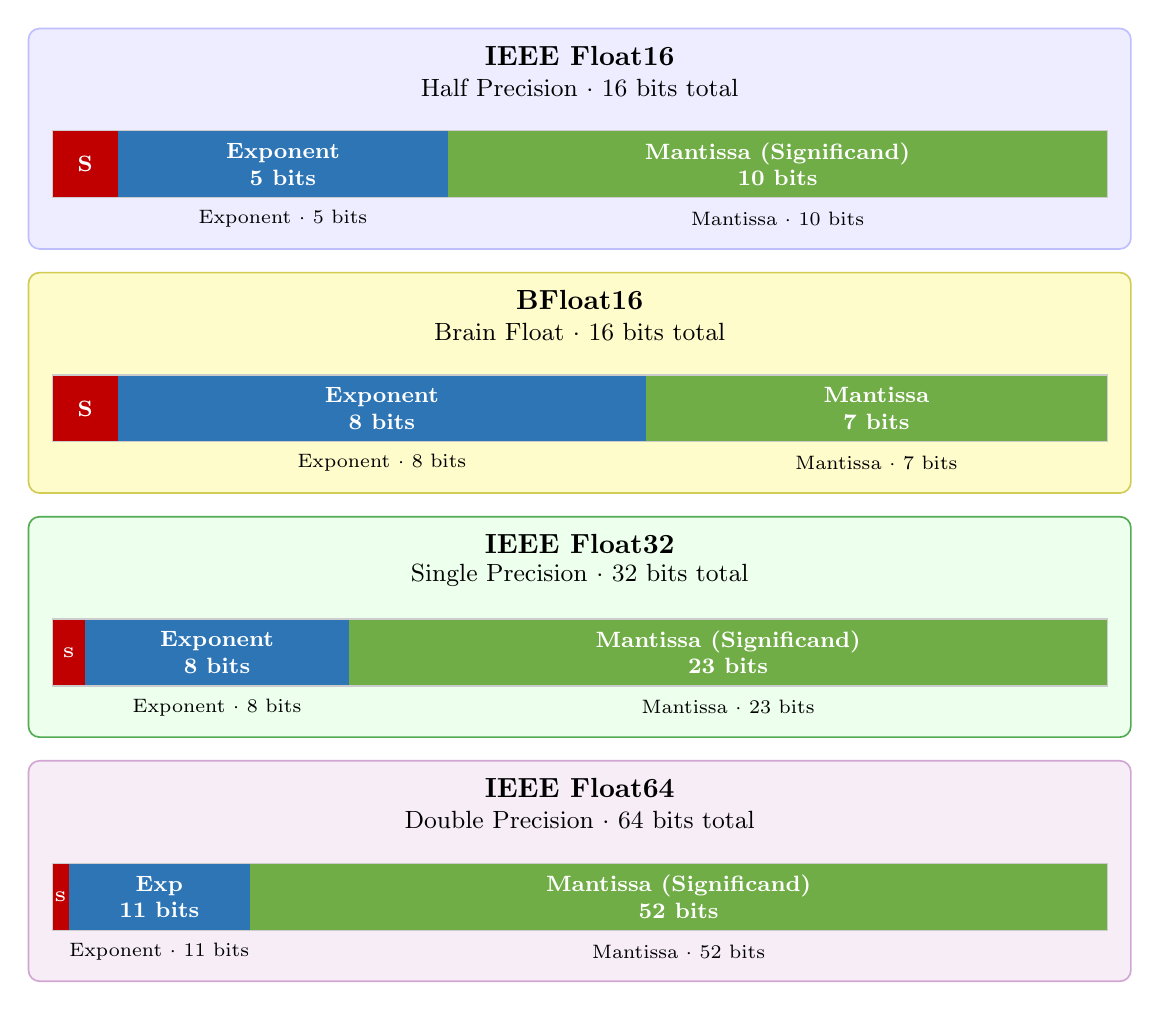
\begin{tikzpicture}[x=1cm, y=1cm]

  % ---- Color palette ----
  \definecolor{signcolor}{RGB}{192,0,0}     % red   -- sign bit
  \definecolor{expcolor} {RGB}{46,117,182}  % blue  -- exponent
  \definecolor{mancolor} {RGB}{112,173,71}  % green -- mantissa

  % ---- Panel backgrounds ----
  % Panels are 14 cm wide x 2.8 cm tall, separated by 0.3 cm gaps.
  % Y positions (bottom edge): Float16=9.30, BFloat16=6.20, Float32=3.10, Float64=0.00
  \draw[rounded corners=4pt, fill=blue!7,    draw=blue!25,        line width=0.6pt]
      (0.0,  9.30) rectangle (14.0, 12.10);  % Float16
  \draw[rounded corners=4pt, fill=yellow!20, draw=yellow!60!gray, line width=0.6pt]
      (0.0,  6.20) rectangle (14.0,  9.00);  % BFloat16
  \draw[rounded corners=4pt, fill=green!7,   draw=green!35!gray,  line width=0.6pt]
      (0.0,  3.10) rectangle (14.0,  5.90);  % Float32
  \draw[rounded corners=4pt, fill=violet!7,  draw=violet!35,      line width=0.6pt]
      (0.0,  0.00) rectangle (14.0,  2.80);  % Float64

  % ====================================================================
  % Bar geometry (shared across all panels):
  %   x range:    [0.30, 13.70]  => total bar width = 13.40 cm
  %   bar height: 0.85 cm
  %   bar bottom: panel_bottom + 0.65
  %   bar top:    panel_bottom + 1.50
  %
  % Segment x boundaries  (width = n_bits/total * 13.40):
  %   Float16  (16-bit): 0.300 | 1.138 | 5.325 | 13.700
  %   BFloat16 (16-bit): 0.300 | 1.138 | 7.838 | 13.700
  %   Float32  (32-bit): 0.300 | 0.719 | 4.069 | 13.700
  %   Float64  (64-bit): 0.300 | 0.509 | 2.813 | 13.700
  % ====================================================================

  % ------------------------------------------------------------------
  % IEEE Float16  (panel bottom y = 9.30)
  % ------------------------------------------------------------------
  \node[font=\normalsize\bfseries] at (7.0, 11.75) {IEEE Float16};
  \node[font=\small]               at (7.0, 11.35) {Half Precision $\cdot$ 16 bits total};

  % S:   1/16 * 13.40 = 0.838 cm   x: 0.300 -- 1.138,  center: 0.719
  \fill[signcolor] (0.300,  9.95) rectangle ( 1.138, 10.80);
  \node[text=white, font=\footnotesize\bfseries] at (0.719, 10.375) {S};

  % Exp: 5/16 * 13.40 = 4.188 cm   x: 1.138 -- 5.325,  center: 3.231
  \fill[expcolor]  (1.138,  9.95) rectangle ( 5.325, 10.80);
  \node[text=white, font=\footnotesize\bfseries, align=center] at (3.231, 10.375)
      {Exponent \\ 5 bits};

  % Man: 10/16 * 13.40 = 8.375 cm  x: 5.325 -- 13.700, center: 9.513
  \fill[mancolor]  (5.325,  9.95) rectangle (13.700, 10.80);
  \node[text=white, font=\footnotesize\bfseries, align=center] at (9.513, 10.375)
      {Mantissa (Significand) \\ 10 bits};

  \draw[black!20, line width=0.4pt] (0.300, 9.95) rectangle (13.700, 10.80);

  \node[font=\scriptsize] at (3.231, 9.68) {Exponent $\cdot$ 5 bits};
  \node[font=\scriptsize] at (9.513, 9.68) {Mantissa $\cdot$ 10 bits};

  % ------------------------------------------------------------------
  % BFloat16  (panel bottom y = 6.20)
  % ------------------------------------------------------------------
  \node[font=\normalsize\bfseries] at (7.0, 8.65) {BFloat16};
  \node[font=\small]               at (7.0, 8.25) {Brain Float $\cdot$ 16 bits total};

  % S:   1/16 * 13.40 = 0.838 cm   x: 0.300 -- 1.138,  center: 0.719
  \fill[signcolor] (0.300,  6.85) rectangle ( 1.138,  7.70);
  \node[text=white, font=\footnotesize\bfseries] at (0.719, 7.275) {S};

  % Exp: 8/16 * 13.40 = 6.700 cm   x: 1.138 -- 7.838,  center: 4.488
  \fill[expcolor]  (1.138,  6.85) rectangle ( 7.838,  7.70);
  \node[text=white, font=\footnotesize\bfseries, align=center] at (4.488, 7.275)
      {Exponent \\ 8 bits};

  % Man: 7/16 * 13.40 = 5.863 cm   x: 7.838 -- 13.700, center: 10.769
  \fill[mancolor]  (7.838,  6.85) rectangle (13.700,  7.70);
  \node[text=white, font=\footnotesize\bfseries, align=center] at (10.769, 7.275)
      {Mantissa \\ 7 bits};

  \draw[black!20, line width=0.4pt] (0.300, 6.85) rectangle (13.700, 7.70);

  \node[font=\scriptsize] at ( 4.488, 6.58) {Exponent $\cdot$ 8 bits};
  \node[font=\scriptsize] at (10.769, 6.58) {Mantissa $\cdot$ 7 bits};

  % ------------------------------------------------------------------
  % IEEE Float32  (panel bottom y = 3.10)
  % ------------------------------------------------------------------
  \node[font=\normalsize\bfseries] at (7.0, 5.55) {IEEE Float32};
  \node[font=\small]               at (7.0, 5.15) {Single Precision $\cdot$ 32 bits total};

  % S:   1/32 * 13.40 = 0.419 cm   x: 0.300 -- 0.719,  center: 0.510
  \fill[signcolor] (0.300,  3.75) rectangle ( 0.719,  4.60);
  \node[text=white, font=\tiny\bfseries] at (0.510, 4.175) {S};

  % Exp: 8/32 * 13.40 = 3.350 cm   x: 0.719 -- 4.069,  center: 2.394
  \fill[expcolor]  (0.719,  3.75) rectangle ( 4.069,  4.60);
  \node[text=white, font=\footnotesize\bfseries, align=center] at (2.394, 4.175)
      {Exponent \\ 8 bits};

  % Man: 23/32 * 13.40 = 9.631 cm  x: 4.069 -- 13.700, center: 8.885
  \fill[mancolor]  (4.069,  3.75) rectangle (13.700,  4.60);
  \node[text=white, font=\footnotesize\bfseries, align=center] at (8.885, 4.175)
      {Mantissa (Significand) \\ 23 bits};

  \draw[black!20, line width=0.4pt] (0.300, 3.75) rectangle (13.700, 4.60);

  \node[font=\scriptsize] at (2.394, 3.48) {Exponent $\cdot$ 8 bits};
  \node[font=\scriptsize] at (8.885, 3.48) {Mantissa $\cdot$ 23 bits};

  % ------------------------------------------------------------------
  % IEEE Float64  (panel bottom y = 0.00)
  % ------------------------------------------------------------------
  \node[font=\normalsize\bfseries] at (7.0, 2.45) {IEEE Float64};
  \node[font=\small]               at (7.0, 2.05) {Double Precision $\cdot$ 64 bits total};

  % S:    1/64 * 13.40 = 0.209 cm  x: 0.300 -- 0.509,  center: 0.405
  \fill[signcolor] (0.300,  0.65) rectangle ( 0.509,  1.50);
  \node[text=white, font=\tiny\bfseries] at (0.405, 1.075) {S};

  % Exp: 11/64 * 13.40 = 2.303 cm  x: 0.509 -- 2.813,  center: 1.661
  \fill[expcolor]  (0.509,  0.65) rectangle ( 2.813,  1.50);
  \node[text=white, font=\footnotesize\bfseries, align=center] at (1.661, 1.075)
      {Exp \\ 11 bits};

  % Man: 52/64 * 13.40 = 10.888 cm x: 2.813 -- 13.700, center: 8.257
  \fill[mancolor]  (2.813,  0.65) rectangle (13.700,  1.50);
  \node[text=white, font=\footnotesize\bfseries, align=center] at (8.257, 1.075)
      {Mantissa (Significand) \\ 52 bits};

  \draw[black!20, line width=0.4pt] (0.300, 0.65) rectangle (13.700, 1.50);

  \node[font=\scriptsize] at (1.661, 0.38) {Exponent $\cdot$ 11 bits};
  \node[font=\scriptsize] at (8.257, 0.38) {Mantissa $\cdot$ 52 bits};

\end{tikzpicture}
}
%
% \resizebox scales everything uniformly — coordinates, line widths,
% and fonts — so the result looks identical regardless of the chosen width.
%
% Recommended figure wrapper (single column):
%   \begin{figure}[t]
%     \centering
%     \resizebox{\columnwidth}{!}{% Floating-point format comparison — single-column stack layout
%
% Required in preamble:
%   \usepackage{tikz}
%
% ---- Scaling -------------------------------------------------------
% The tikzpicture is drawn at its natural size: 14 cm wide x 12.1 cm tall.
% Use \resizebox (from the graphicx package, always loaded in IEEE style)
% to scale it to whatever width you need. The height adjusts automatically.
%
%   Fit to a single text column (~8.8 cm in IEEE two-column):
%     \resizebox{\columnwidth}{!}{\input{float_formats_tikz.tex}}
%
%   Fit to the full page width (~17.8 cm in IEEE two-column):
%     \resizebox{\textwidth}{!}{\input{float_formats_tikz.tex}}
%
%   Fit to an arbitrary fraction of the column width:
%     \resizebox{0.9\columnwidth}{!}{\input{float_formats_tikz.tex}}
%
% \resizebox scales everything uniformly — coordinates, line widths,
% and fonts — so the result looks identical regardless of the chosen width.
%
% Recommended figure wrapper (single column):
%   \begin{figure}[t]
%     \centering
%     \resizebox{\columnwidth}{!}{\input{float_formats_tikz.tex}}
%     \caption{...}
%     \label{fig:float-formats}
%   \end{figure}
% --------------------------------------------------------------------
%
% Layout: 4 panels stacked vertically, each 14 cm x 2.8 cm.
% Bar widths are proportional to actual bit-field widths.
%   Float16:  S=1, Exp=5,  Man=10  (16 bits total)
%   BFloat16: S=1, Exp=8,  Man=7   (16 bits total)
%   Float32:  S=1, Exp=8,  Man=23  (32 bits total)
%   Float64:  S=1, Exp=11, Man=52  (64 bits total)

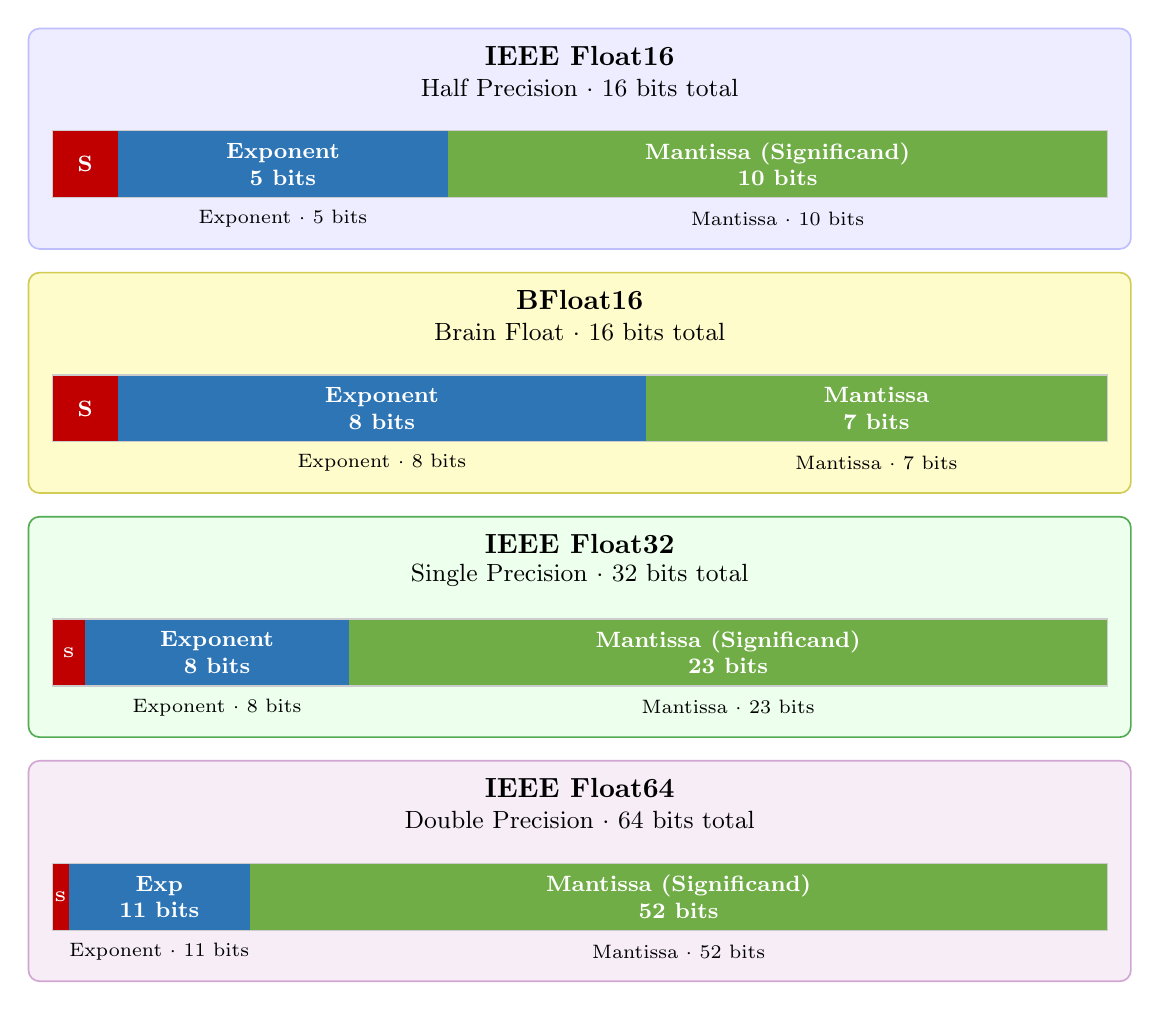
\begin{tikzpicture}[x=1cm, y=1cm]

  % ---- Color palette ----
  \definecolor{signcolor}{RGB}{192,0,0}     % red   -- sign bit
  \definecolor{expcolor} {RGB}{46,117,182}  % blue  -- exponent
  \definecolor{mancolor} {RGB}{112,173,71}  % green -- mantissa

  % ---- Panel backgrounds ----
  % Panels are 14 cm wide x 2.8 cm tall, separated by 0.3 cm gaps.
  % Y positions (bottom edge): Float16=9.30, BFloat16=6.20, Float32=3.10, Float64=0.00
  \draw[rounded corners=4pt, fill=blue!7,    draw=blue!25,        line width=0.6pt]
      (0.0,  9.30) rectangle (14.0, 12.10);  % Float16
  \draw[rounded corners=4pt, fill=yellow!20, draw=yellow!60!gray, line width=0.6pt]
      (0.0,  6.20) rectangle (14.0,  9.00);  % BFloat16
  \draw[rounded corners=4pt, fill=green!7,   draw=green!35!gray,  line width=0.6pt]
      (0.0,  3.10) rectangle (14.0,  5.90);  % Float32
  \draw[rounded corners=4pt, fill=violet!7,  draw=violet!35,      line width=0.6pt]
      (0.0,  0.00) rectangle (14.0,  2.80);  % Float64

  % ====================================================================
  % Bar geometry (shared across all panels):
  %   x range:    [0.30, 13.70]  => total bar width = 13.40 cm
  %   bar height: 0.85 cm
  %   bar bottom: panel_bottom + 0.65
  %   bar top:    panel_bottom + 1.50
  %
  % Segment x boundaries  (width = n_bits/total * 13.40):
  %   Float16  (16-bit): 0.300 | 1.138 | 5.325 | 13.700
  %   BFloat16 (16-bit): 0.300 | 1.138 | 7.838 | 13.700
  %   Float32  (32-bit): 0.300 | 0.719 | 4.069 | 13.700
  %   Float64  (64-bit): 0.300 | 0.509 | 2.813 | 13.700
  % ====================================================================

  % ------------------------------------------------------------------
  % IEEE Float16  (panel bottom y = 9.30)
  % ------------------------------------------------------------------
  \node[font=\normalsize\bfseries] at (7.0, 11.75) {IEEE Float16};
  \node[font=\small]               at (7.0, 11.35) {Half Precision $\cdot$ 16 bits total};

  % S:   1/16 * 13.40 = 0.838 cm   x: 0.300 -- 1.138,  center: 0.719
  \fill[signcolor] (0.300,  9.95) rectangle ( 1.138, 10.80);
  \node[text=white, font=\footnotesize\bfseries] at (0.719, 10.375) {S};

  % Exp: 5/16 * 13.40 = 4.188 cm   x: 1.138 -- 5.325,  center: 3.231
  \fill[expcolor]  (1.138,  9.95) rectangle ( 5.325, 10.80);
  \node[text=white, font=\footnotesize\bfseries, align=center] at (3.231, 10.375)
      {Exponent \\ 5 bits};

  % Man: 10/16 * 13.40 = 8.375 cm  x: 5.325 -- 13.700, center: 9.513
  \fill[mancolor]  (5.325,  9.95) rectangle (13.700, 10.80);
  \node[text=white, font=\footnotesize\bfseries, align=center] at (9.513, 10.375)
      {Mantissa (Significand) \\ 10 bits};

  \draw[black!20, line width=0.4pt] (0.300, 9.95) rectangle (13.700, 10.80);

  \node[font=\scriptsize] at (3.231, 9.68) {Exponent $\cdot$ 5 bits};
  \node[font=\scriptsize] at (9.513, 9.68) {Mantissa $\cdot$ 10 bits};

  % ------------------------------------------------------------------
  % BFloat16  (panel bottom y = 6.20)
  % ------------------------------------------------------------------
  \node[font=\normalsize\bfseries] at (7.0, 8.65) {BFloat16};
  \node[font=\small]               at (7.0, 8.25) {Brain Float $\cdot$ 16 bits total};

  % S:   1/16 * 13.40 = 0.838 cm   x: 0.300 -- 1.138,  center: 0.719
  \fill[signcolor] (0.300,  6.85) rectangle ( 1.138,  7.70);
  \node[text=white, font=\footnotesize\bfseries] at (0.719, 7.275) {S};

  % Exp: 8/16 * 13.40 = 6.700 cm   x: 1.138 -- 7.838,  center: 4.488
  \fill[expcolor]  (1.138,  6.85) rectangle ( 7.838,  7.70);
  \node[text=white, font=\footnotesize\bfseries, align=center] at (4.488, 7.275)
      {Exponent \\ 8 bits};

  % Man: 7/16 * 13.40 = 5.863 cm   x: 7.838 -- 13.700, center: 10.769
  \fill[mancolor]  (7.838,  6.85) rectangle (13.700,  7.70);
  \node[text=white, font=\footnotesize\bfseries, align=center] at (10.769, 7.275)
      {Mantissa \\ 7 bits};

  \draw[black!20, line width=0.4pt] (0.300, 6.85) rectangle (13.700, 7.70);

  \node[font=\scriptsize] at ( 4.488, 6.58) {Exponent $\cdot$ 8 bits};
  \node[font=\scriptsize] at (10.769, 6.58) {Mantissa $\cdot$ 7 bits};

  % ------------------------------------------------------------------
  % IEEE Float32  (panel bottom y = 3.10)
  % ------------------------------------------------------------------
  \node[font=\normalsize\bfseries] at (7.0, 5.55) {IEEE Float32};
  \node[font=\small]               at (7.0, 5.15) {Single Precision $\cdot$ 32 bits total};

  % S:   1/32 * 13.40 = 0.419 cm   x: 0.300 -- 0.719,  center: 0.510
  \fill[signcolor] (0.300,  3.75) rectangle ( 0.719,  4.60);
  \node[text=white, font=\tiny\bfseries] at (0.510, 4.175) {S};

  % Exp: 8/32 * 13.40 = 3.350 cm   x: 0.719 -- 4.069,  center: 2.394
  \fill[expcolor]  (0.719,  3.75) rectangle ( 4.069,  4.60);
  \node[text=white, font=\footnotesize\bfseries, align=center] at (2.394, 4.175)
      {Exponent \\ 8 bits};

  % Man: 23/32 * 13.40 = 9.631 cm  x: 4.069 -- 13.700, center: 8.885
  \fill[mancolor]  (4.069,  3.75) rectangle (13.700,  4.60);
  \node[text=white, font=\footnotesize\bfseries, align=center] at (8.885, 4.175)
      {Mantissa (Significand) \\ 23 bits};

  \draw[black!20, line width=0.4pt] (0.300, 3.75) rectangle (13.700, 4.60);

  \node[font=\scriptsize] at (2.394, 3.48) {Exponent $\cdot$ 8 bits};
  \node[font=\scriptsize] at (8.885, 3.48) {Mantissa $\cdot$ 23 bits};

  % ------------------------------------------------------------------
  % IEEE Float64  (panel bottom y = 0.00)
  % ------------------------------------------------------------------
  \node[font=\normalsize\bfseries] at (7.0, 2.45) {IEEE Float64};
  \node[font=\small]               at (7.0, 2.05) {Double Precision $\cdot$ 64 bits total};

  % S:    1/64 * 13.40 = 0.209 cm  x: 0.300 -- 0.509,  center: 0.405
  \fill[signcolor] (0.300,  0.65) rectangle ( 0.509,  1.50);
  \node[text=white, font=\tiny\bfseries] at (0.405, 1.075) {S};

  % Exp: 11/64 * 13.40 = 2.303 cm  x: 0.509 -- 2.813,  center: 1.661
  \fill[expcolor]  (0.509,  0.65) rectangle ( 2.813,  1.50);
  \node[text=white, font=\footnotesize\bfseries, align=center] at (1.661, 1.075)
      {Exp \\ 11 bits};

  % Man: 52/64 * 13.40 = 10.888 cm x: 2.813 -- 13.700, center: 8.257
  \fill[mancolor]  (2.813,  0.65) rectangle (13.700,  1.50);
  \node[text=white, font=\footnotesize\bfseries, align=center] at (8.257, 1.075)
      {Mantissa (Significand) \\ 52 bits};

  \draw[black!20, line width=0.4pt] (0.300, 0.65) rectangle (13.700, 1.50);

  \node[font=\scriptsize] at (1.661, 0.38) {Exponent $\cdot$ 11 bits};
  \node[font=\scriptsize] at (8.257, 0.38) {Mantissa $\cdot$ 52 bits};

\end{tikzpicture}
}
%     \caption{...}
%     \label{fig:float-formats}
%   \end{figure}
% --------------------------------------------------------------------
%
% Layout: 4 panels stacked vertically, each 14 cm x 2.8 cm.
% Bar widths are proportional to actual bit-field widths.
%   Float16:  S=1, Exp=5,  Man=10  (16 bits total)
%   BFloat16: S=1, Exp=8,  Man=7   (16 bits total)
%   Float32:  S=1, Exp=8,  Man=23  (32 bits total)
%   Float64:  S=1, Exp=11, Man=52  (64 bits total)

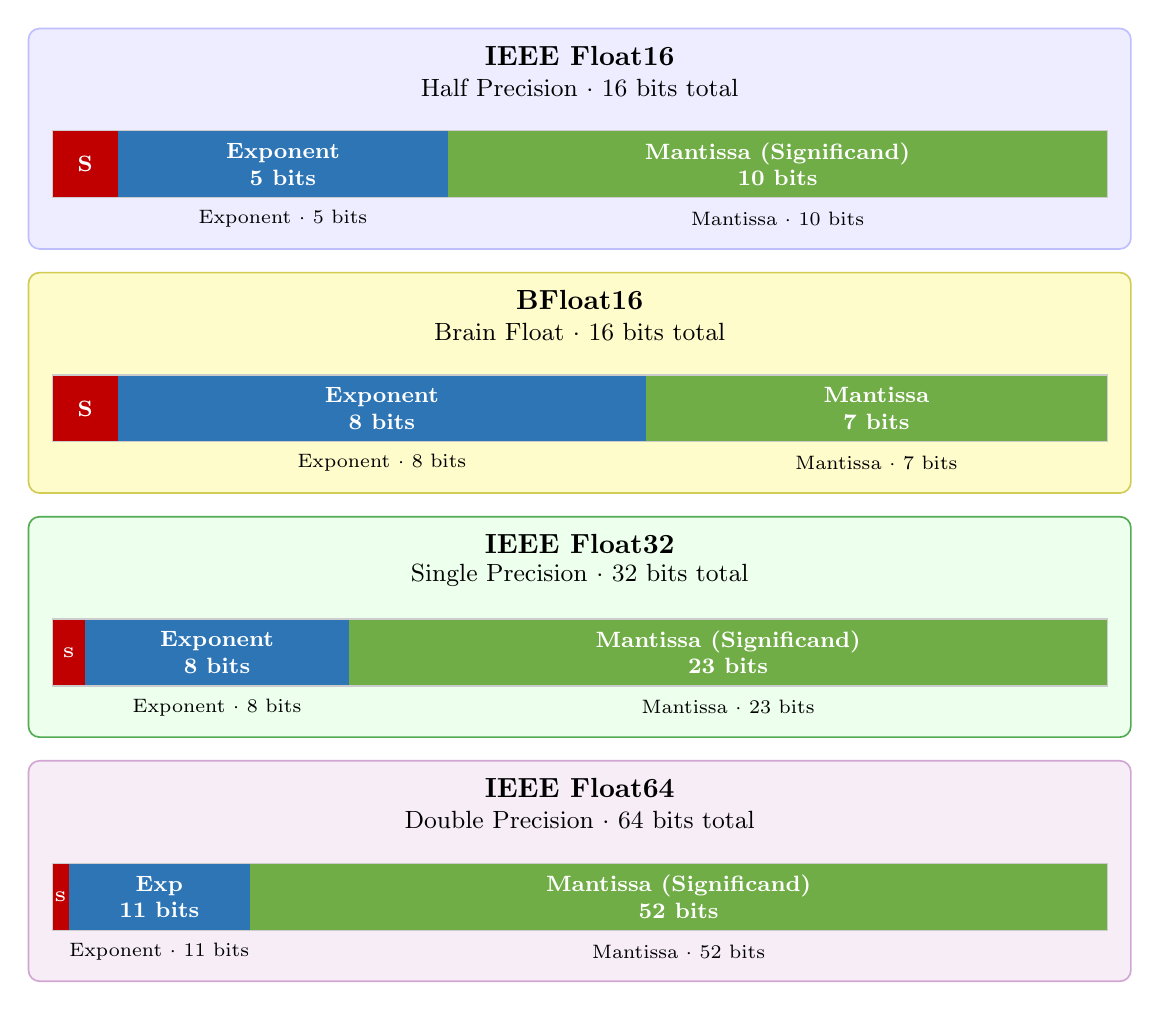
\begin{tikzpicture}[x=1cm, y=1cm]

  % ---- Color palette ----
  \definecolor{signcolor}{RGB}{192,0,0}     % red   -- sign bit
  \definecolor{expcolor} {RGB}{46,117,182}  % blue  -- exponent
  \definecolor{mancolor} {RGB}{112,173,71}  % green -- mantissa

  % ---- Panel backgrounds ----
  % Panels are 14 cm wide x 2.8 cm tall, separated by 0.3 cm gaps.
  % Y positions (bottom edge): Float16=9.30, BFloat16=6.20, Float32=3.10, Float64=0.00
  \draw[rounded corners=4pt, fill=blue!7,    draw=blue!25,        line width=0.6pt]
      (0.0,  9.30) rectangle (14.0, 12.10);  % Float16
  \draw[rounded corners=4pt, fill=yellow!20, draw=yellow!60!gray, line width=0.6pt]
      (0.0,  6.20) rectangle (14.0,  9.00);  % BFloat16
  \draw[rounded corners=4pt, fill=green!7,   draw=green!35!gray,  line width=0.6pt]
      (0.0,  3.10) rectangle (14.0,  5.90);  % Float32
  \draw[rounded corners=4pt, fill=violet!7,  draw=violet!35,      line width=0.6pt]
      (0.0,  0.00) rectangle (14.0,  2.80);  % Float64

  % ====================================================================
  % Bar geometry (shared across all panels):
  %   x range:    [0.30, 13.70]  => total bar width = 13.40 cm
  %   bar height: 0.85 cm
  %   bar bottom: panel_bottom + 0.65
  %   bar top:    panel_bottom + 1.50
  %
  % Segment x boundaries  (width = n_bits/total * 13.40):
  %   Float16  (16-bit): 0.300 | 1.138 | 5.325 | 13.700
  %   BFloat16 (16-bit): 0.300 | 1.138 | 7.838 | 13.700
  %   Float32  (32-bit): 0.300 | 0.719 | 4.069 | 13.700
  %   Float64  (64-bit): 0.300 | 0.509 | 2.813 | 13.700
  % ====================================================================

  % ------------------------------------------------------------------
  % IEEE Float16  (panel bottom y = 9.30)
  % ------------------------------------------------------------------
  \node[font=\normalsize\bfseries] at (7.0, 11.75) {IEEE Float16};
  \node[font=\small]               at (7.0, 11.35) {Half Precision $\cdot$ 16 bits total};

  % S:   1/16 * 13.40 = 0.838 cm   x: 0.300 -- 1.138,  center: 0.719
  \fill[signcolor] (0.300,  9.95) rectangle ( 1.138, 10.80);
  \node[text=white, font=\footnotesize\bfseries] at (0.719, 10.375) {S};

  % Exp: 5/16 * 13.40 = 4.188 cm   x: 1.138 -- 5.325,  center: 3.231
  \fill[expcolor]  (1.138,  9.95) rectangle ( 5.325, 10.80);
  \node[text=white, font=\footnotesize\bfseries, align=center] at (3.231, 10.375)
      {Exponent \\ 5 bits};

  % Man: 10/16 * 13.40 = 8.375 cm  x: 5.325 -- 13.700, center: 9.513
  \fill[mancolor]  (5.325,  9.95) rectangle (13.700, 10.80);
  \node[text=white, font=\footnotesize\bfseries, align=center] at (9.513, 10.375)
      {Mantissa (Significand) \\ 10 bits};

  \draw[black!20, line width=0.4pt] (0.300, 9.95) rectangle (13.700, 10.80);

  \node[font=\scriptsize] at (3.231, 9.68) {Exponent $\cdot$ 5 bits};
  \node[font=\scriptsize] at (9.513, 9.68) {Mantissa $\cdot$ 10 bits};

  % ------------------------------------------------------------------
  % BFloat16  (panel bottom y = 6.20)
  % ------------------------------------------------------------------
  \node[font=\normalsize\bfseries] at (7.0, 8.65) {BFloat16};
  \node[font=\small]               at (7.0, 8.25) {Brain Float $\cdot$ 16 bits total};

  % S:   1/16 * 13.40 = 0.838 cm   x: 0.300 -- 1.138,  center: 0.719
  \fill[signcolor] (0.300,  6.85) rectangle ( 1.138,  7.70);
  \node[text=white, font=\footnotesize\bfseries] at (0.719, 7.275) {S};

  % Exp: 8/16 * 13.40 = 6.700 cm   x: 1.138 -- 7.838,  center: 4.488
  \fill[expcolor]  (1.138,  6.85) rectangle ( 7.838,  7.70);
  \node[text=white, font=\footnotesize\bfseries, align=center] at (4.488, 7.275)
      {Exponent \\ 8 bits};

  % Man: 7/16 * 13.40 = 5.863 cm   x: 7.838 -- 13.700, center: 10.769
  \fill[mancolor]  (7.838,  6.85) rectangle (13.700,  7.70);
  \node[text=white, font=\footnotesize\bfseries, align=center] at (10.769, 7.275)
      {Mantissa \\ 7 bits};

  \draw[black!20, line width=0.4pt] (0.300, 6.85) rectangle (13.700, 7.70);

  \node[font=\scriptsize] at ( 4.488, 6.58) {Exponent $\cdot$ 8 bits};
  \node[font=\scriptsize] at (10.769, 6.58) {Mantissa $\cdot$ 7 bits};

  % ------------------------------------------------------------------
  % IEEE Float32  (panel bottom y = 3.10)
  % ------------------------------------------------------------------
  \node[font=\normalsize\bfseries] at (7.0, 5.55) {IEEE Float32};
  \node[font=\small]               at (7.0, 5.15) {Single Precision $\cdot$ 32 bits total};

  % S:   1/32 * 13.40 = 0.419 cm   x: 0.300 -- 0.719,  center: 0.510
  \fill[signcolor] (0.300,  3.75) rectangle ( 0.719,  4.60);
  \node[text=white, font=\tiny\bfseries] at (0.510, 4.175) {S};

  % Exp: 8/32 * 13.40 = 3.350 cm   x: 0.719 -- 4.069,  center: 2.394
  \fill[expcolor]  (0.719,  3.75) rectangle ( 4.069,  4.60);
  \node[text=white, font=\footnotesize\bfseries, align=center] at (2.394, 4.175)
      {Exponent \\ 8 bits};

  % Man: 23/32 * 13.40 = 9.631 cm  x: 4.069 -- 13.700, center: 8.885
  \fill[mancolor]  (4.069,  3.75) rectangle (13.700,  4.60);
  \node[text=white, font=\footnotesize\bfseries, align=center] at (8.885, 4.175)
      {Mantissa (Significand) \\ 23 bits};

  \draw[black!20, line width=0.4pt] (0.300, 3.75) rectangle (13.700, 4.60);

  \node[font=\scriptsize] at (2.394, 3.48) {Exponent $\cdot$ 8 bits};
  \node[font=\scriptsize] at (8.885, 3.48) {Mantissa $\cdot$ 23 bits};

  % ------------------------------------------------------------------
  % IEEE Float64  (panel bottom y = 0.00)
  % ------------------------------------------------------------------
  \node[font=\normalsize\bfseries] at (7.0, 2.45) {IEEE Float64};
  \node[font=\small]               at (7.0, 2.05) {Double Precision $\cdot$ 64 bits total};

  % S:    1/64 * 13.40 = 0.209 cm  x: 0.300 -- 0.509,  center: 0.405
  \fill[signcolor] (0.300,  0.65) rectangle ( 0.509,  1.50);
  \node[text=white, font=\tiny\bfseries] at (0.405, 1.075) {S};

  % Exp: 11/64 * 13.40 = 2.303 cm  x: 0.509 -- 2.813,  center: 1.661
  \fill[expcolor]  (0.509,  0.65) rectangle ( 2.813,  1.50);
  \node[text=white, font=\footnotesize\bfseries, align=center] at (1.661, 1.075)
      {Exp \\ 11 bits};

  % Man: 52/64 * 13.40 = 10.888 cm x: 2.813 -- 13.700, center: 8.257
  \fill[mancolor]  (2.813,  0.65) rectangle (13.700,  1.50);
  \node[text=white, font=\footnotesize\bfseries, align=center] at (8.257, 1.075)
      {Mantissa (Significand) \\ 52 bits};

  \draw[black!20, line width=0.4pt] (0.300, 0.65) rectangle (13.700, 1.50);

  \node[font=\scriptsize] at (1.661, 0.38) {Exponent $\cdot$ 11 bits};
  \node[font=\scriptsize] at (8.257, 0.38) {Mantissa $\cdot$ 52 bits};

\end{tikzpicture}
}
%
%   Fit to an arbitrary fraction of the column width:
%     \resizebox{0.9\columnwidth}{!}{% Floating-point format comparison — single-column stack layout
%
% Required in preamble:
%   \usepackage{tikz}
%
% ---- Scaling -------------------------------------------------------
% The tikzpicture is drawn at its natural size: 14 cm wide x 12.1 cm tall.
% Use \resizebox (from the graphicx package, always loaded in IEEE style)
% to scale it to whatever width you need. The height adjusts automatically.
%
%   Fit to a single text column (~8.8 cm in IEEE two-column):
%     \resizebox{\columnwidth}{!}{% Floating-point format comparison — single-column stack layout
%
% Required in preamble:
%   \usepackage{tikz}
%
% ---- Scaling -------------------------------------------------------
% The tikzpicture is drawn at its natural size: 14 cm wide x 12.1 cm tall.
% Use \resizebox (from the graphicx package, always loaded in IEEE style)
% to scale it to whatever width you need. The height adjusts automatically.
%
%   Fit to a single text column (~8.8 cm in IEEE two-column):
%     \resizebox{\columnwidth}{!}{\input{float_formats_tikz.tex}}
%
%   Fit to the full page width (~17.8 cm in IEEE two-column):
%     \resizebox{\textwidth}{!}{\input{float_formats_tikz.tex}}
%
%   Fit to an arbitrary fraction of the column width:
%     \resizebox{0.9\columnwidth}{!}{\input{float_formats_tikz.tex}}
%
% \resizebox scales everything uniformly — coordinates, line widths,
% and fonts — so the result looks identical regardless of the chosen width.
%
% Recommended figure wrapper (single column):
%   \begin{figure}[t]
%     \centering
%     \resizebox{\columnwidth}{!}{\input{float_formats_tikz.tex}}
%     \caption{...}
%     \label{fig:float-formats}
%   \end{figure}
% --------------------------------------------------------------------
%
% Layout: 4 panels stacked vertically, each 14 cm x 2.8 cm.
% Bar widths are proportional to actual bit-field widths.
%   Float16:  S=1, Exp=5,  Man=10  (16 bits total)
%   BFloat16: S=1, Exp=8,  Man=7   (16 bits total)
%   Float32:  S=1, Exp=8,  Man=23  (32 bits total)
%   Float64:  S=1, Exp=11, Man=52  (64 bits total)

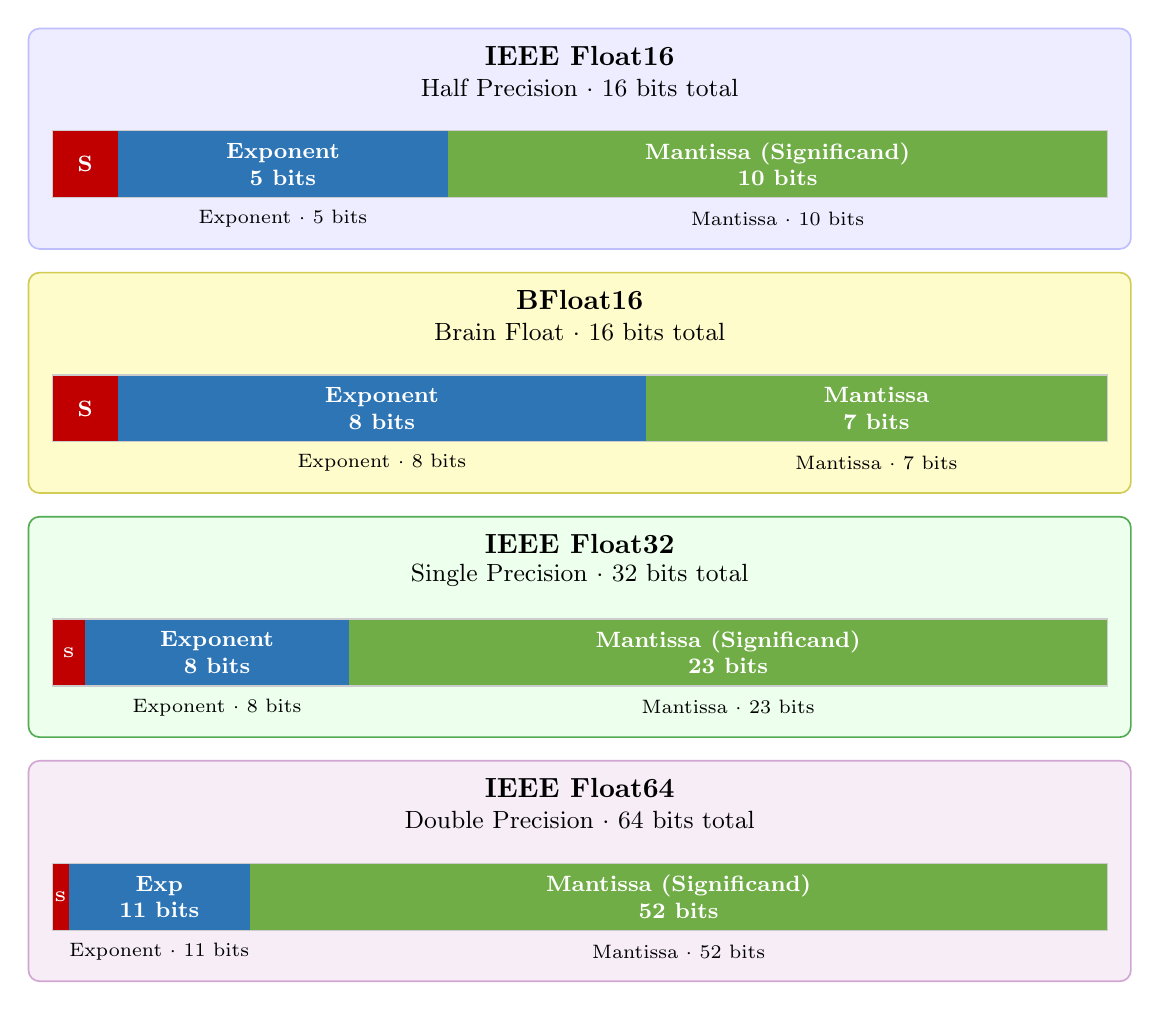
\begin{tikzpicture}[x=1cm, y=1cm]

  % ---- Color palette ----
  \definecolor{signcolor}{RGB}{192,0,0}     % red   -- sign bit
  \definecolor{expcolor} {RGB}{46,117,182}  % blue  -- exponent
  \definecolor{mancolor} {RGB}{112,173,71}  % green -- mantissa

  % ---- Panel backgrounds ----
  % Panels are 14 cm wide x 2.8 cm tall, separated by 0.3 cm gaps.
  % Y positions (bottom edge): Float16=9.30, BFloat16=6.20, Float32=3.10, Float64=0.00
  \draw[rounded corners=4pt, fill=blue!7,    draw=blue!25,        line width=0.6pt]
      (0.0,  9.30) rectangle (14.0, 12.10);  % Float16
  \draw[rounded corners=4pt, fill=yellow!20, draw=yellow!60!gray, line width=0.6pt]
      (0.0,  6.20) rectangle (14.0,  9.00);  % BFloat16
  \draw[rounded corners=4pt, fill=green!7,   draw=green!35!gray,  line width=0.6pt]
      (0.0,  3.10) rectangle (14.0,  5.90);  % Float32
  \draw[rounded corners=4pt, fill=violet!7,  draw=violet!35,      line width=0.6pt]
      (0.0,  0.00) rectangle (14.0,  2.80);  % Float64

  % ====================================================================
  % Bar geometry (shared across all panels):
  %   x range:    [0.30, 13.70]  => total bar width = 13.40 cm
  %   bar height: 0.85 cm
  %   bar bottom: panel_bottom + 0.65
  %   bar top:    panel_bottom + 1.50
  %
  % Segment x boundaries  (width = n_bits/total * 13.40):
  %   Float16  (16-bit): 0.300 | 1.138 | 5.325 | 13.700
  %   BFloat16 (16-bit): 0.300 | 1.138 | 7.838 | 13.700
  %   Float32  (32-bit): 0.300 | 0.719 | 4.069 | 13.700
  %   Float64  (64-bit): 0.300 | 0.509 | 2.813 | 13.700
  % ====================================================================

  % ------------------------------------------------------------------
  % IEEE Float16  (panel bottom y = 9.30)
  % ------------------------------------------------------------------
  \node[font=\normalsize\bfseries] at (7.0, 11.75) {IEEE Float16};
  \node[font=\small]               at (7.0, 11.35) {Half Precision $\cdot$ 16 bits total};

  % S:   1/16 * 13.40 = 0.838 cm   x: 0.300 -- 1.138,  center: 0.719
  \fill[signcolor] (0.300,  9.95) rectangle ( 1.138, 10.80);
  \node[text=white, font=\footnotesize\bfseries] at (0.719, 10.375) {S};

  % Exp: 5/16 * 13.40 = 4.188 cm   x: 1.138 -- 5.325,  center: 3.231
  \fill[expcolor]  (1.138,  9.95) rectangle ( 5.325, 10.80);
  \node[text=white, font=\footnotesize\bfseries, align=center] at (3.231, 10.375)
      {Exponent \\ 5 bits};

  % Man: 10/16 * 13.40 = 8.375 cm  x: 5.325 -- 13.700, center: 9.513
  \fill[mancolor]  (5.325,  9.95) rectangle (13.700, 10.80);
  \node[text=white, font=\footnotesize\bfseries, align=center] at (9.513, 10.375)
      {Mantissa (Significand) \\ 10 bits};

  \draw[black!20, line width=0.4pt] (0.300, 9.95) rectangle (13.700, 10.80);

  \node[font=\scriptsize] at (3.231, 9.68) {Exponent $\cdot$ 5 bits};
  \node[font=\scriptsize] at (9.513, 9.68) {Mantissa $\cdot$ 10 bits};

  % ------------------------------------------------------------------
  % BFloat16  (panel bottom y = 6.20)
  % ------------------------------------------------------------------
  \node[font=\normalsize\bfseries] at (7.0, 8.65) {BFloat16};
  \node[font=\small]               at (7.0, 8.25) {Brain Float $\cdot$ 16 bits total};

  % S:   1/16 * 13.40 = 0.838 cm   x: 0.300 -- 1.138,  center: 0.719
  \fill[signcolor] (0.300,  6.85) rectangle ( 1.138,  7.70);
  \node[text=white, font=\footnotesize\bfseries] at (0.719, 7.275) {S};

  % Exp: 8/16 * 13.40 = 6.700 cm   x: 1.138 -- 7.838,  center: 4.488
  \fill[expcolor]  (1.138,  6.85) rectangle ( 7.838,  7.70);
  \node[text=white, font=\footnotesize\bfseries, align=center] at (4.488, 7.275)
      {Exponent \\ 8 bits};

  % Man: 7/16 * 13.40 = 5.863 cm   x: 7.838 -- 13.700, center: 10.769
  \fill[mancolor]  (7.838,  6.85) rectangle (13.700,  7.70);
  \node[text=white, font=\footnotesize\bfseries, align=center] at (10.769, 7.275)
      {Mantissa \\ 7 bits};

  \draw[black!20, line width=0.4pt] (0.300, 6.85) rectangle (13.700, 7.70);

  \node[font=\scriptsize] at ( 4.488, 6.58) {Exponent $\cdot$ 8 bits};
  \node[font=\scriptsize] at (10.769, 6.58) {Mantissa $\cdot$ 7 bits};

  % ------------------------------------------------------------------
  % IEEE Float32  (panel bottom y = 3.10)
  % ------------------------------------------------------------------
  \node[font=\normalsize\bfseries] at (7.0, 5.55) {IEEE Float32};
  \node[font=\small]               at (7.0, 5.15) {Single Precision $\cdot$ 32 bits total};

  % S:   1/32 * 13.40 = 0.419 cm   x: 0.300 -- 0.719,  center: 0.510
  \fill[signcolor] (0.300,  3.75) rectangle ( 0.719,  4.60);
  \node[text=white, font=\tiny\bfseries] at (0.510, 4.175) {S};

  % Exp: 8/32 * 13.40 = 3.350 cm   x: 0.719 -- 4.069,  center: 2.394
  \fill[expcolor]  (0.719,  3.75) rectangle ( 4.069,  4.60);
  \node[text=white, font=\footnotesize\bfseries, align=center] at (2.394, 4.175)
      {Exponent \\ 8 bits};

  % Man: 23/32 * 13.40 = 9.631 cm  x: 4.069 -- 13.700, center: 8.885
  \fill[mancolor]  (4.069,  3.75) rectangle (13.700,  4.60);
  \node[text=white, font=\footnotesize\bfseries, align=center] at (8.885, 4.175)
      {Mantissa (Significand) \\ 23 bits};

  \draw[black!20, line width=0.4pt] (0.300, 3.75) rectangle (13.700, 4.60);

  \node[font=\scriptsize] at (2.394, 3.48) {Exponent $\cdot$ 8 bits};
  \node[font=\scriptsize] at (8.885, 3.48) {Mantissa $\cdot$ 23 bits};

  % ------------------------------------------------------------------
  % IEEE Float64  (panel bottom y = 0.00)
  % ------------------------------------------------------------------
  \node[font=\normalsize\bfseries] at (7.0, 2.45) {IEEE Float64};
  \node[font=\small]               at (7.0, 2.05) {Double Precision $\cdot$ 64 bits total};

  % S:    1/64 * 13.40 = 0.209 cm  x: 0.300 -- 0.509,  center: 0.405
  \fill[signcolor] (0.300,  0.65) rectangle ( 0.509,  1.50);
  \node[text=white, font=\tiny\bfseries] at (0.405, 1.075) {S};

  % Exp: 11/64 * 13.40 = 2.303 cm  x: 0.509 -- 2.813,  center: 1.661
  \fill[expcolor]  (0.509,  0.65) rectangle ( 2.813,  1.50);
  \node[text=white, font=\footnotesize\bfseries, align=center] at (1.661, 1.075)
      {Exp \\ 11 bits};

  % Man: 52/64 * 13.40 = 10.888 cm x: 2.813 -- 13.700, center: 8.257
  \fill[mancolor]  (2.813,  0.65) rectangle (13.700,  1.50);
  \node[text=white, font=\footnotesize\bfseries, align=center] at (8.257, 1.075)
      {Mantissa (Significand) \\ 52 bits};

  \draw[black!20, line width=0.4pt] (0.300, 0.65) rectangle (13.700, 1.50);

  \node[font=\scriptsize] at (1.661, 0.38) {Exponent $\cdot$ 11 bits};
  \node[font=\scriptsize] at (8.257, 0.38) {Mantissa $\cdot$ 52 bits};

\end{tikzpicture}
}
%
%   Fit to the full page width (~17.8 cm in IEEE two-column):
%     \resizebox{\textwidth}{!}{% Floating-point format comparison — single-column stack layout
%
% Required in preamble:
%   \usepackage{tikz}
%
% ---- Scaling -------------------------------------------------------
% The tikzpicture is drawn at its natural size: 14 cm wide x 12.1 cm tall.
% Use \resizebox (from the graphicx package, always loaded in IEEE style)
% to scale it to whatever width you need. The height adjusts automatically.
%
%   Fit to a single text column (~8.8 cm in IEEE two-column):
%     \resizebox{\columnwidth}{!}{\input{float_formats_tikz.tex}}
%
%   Fit to the full page width (~17.8 cm in IEEE two-column):
%     \resizebox{\textwidth}{!}{\input{float_formats_tikz.tex}}
%
%   Fit to an arbitrary fraction of the column width:
%     \resizebox{0.9\columnwidth}{!}{\input{float_formats_tikz.tex}}
%
% \resizebox scales everything uniformly — coordinates, line widths,
% and fonts — so the result looks identical regardless of the chosen width.
%
% Recommended figure wrapper (single column):
%   \begin{figure}[t]
%     \centering
%     \resizebox{\columnwidth}{!}{\input{float_formats_tikz.tex}}
%     \caption{...}
%     \label{fig:float-formats}
%   \end{figure}
% --------------------------------------------------------------------
%
% Layout: 4 panels stacked vertically, each 14 cm x 2.8 cm.
% Bar widths are proportional to actual bit-field widths.
%   Float16:  S=1, Exp=5,  Man=10  (16 bits total)
%   BFloat16: S=1, Exp=8,  Man=7   (16 bits total)
%   Float32:  S=1, Exp=8,  Man=23  (32 bits total)
%   Float64:  S=1, Exp=11, Man=52  (64 bits total)

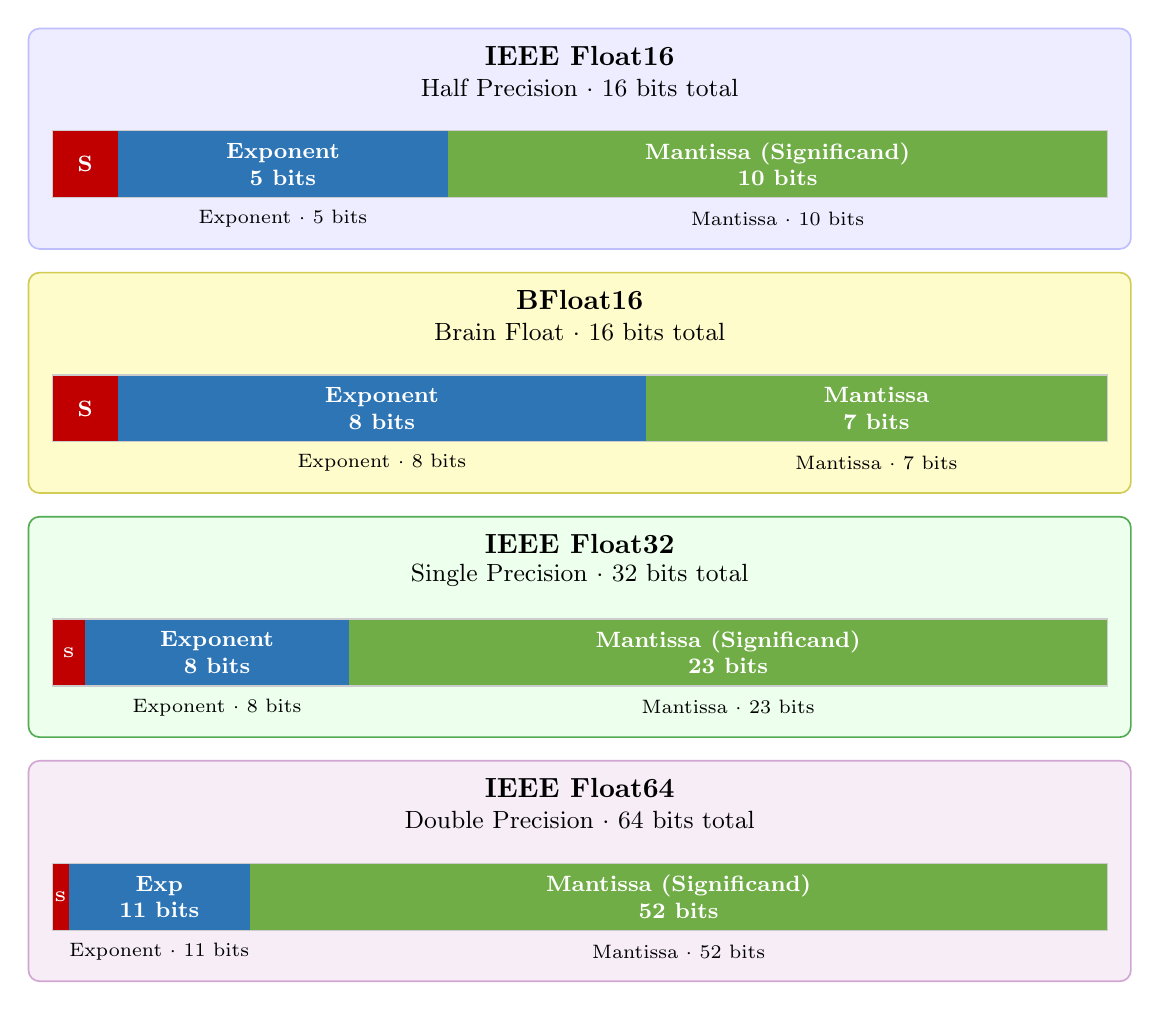
\begin{tikzpicture}[x=1cm, y=1cm]

  % ---- Color palette ----
  \definecolor{signcolor}{RGB}{192,0,0}     % red   -- sign bit
  \definecolor{expcolor} {RGB}{46,117,182}  % blue  -- exponent
  \definecolor{mancolor} {RGB}{112,173,71}  % green -- mantissa

  % ---- Panel backgrounds ----
  % Panels are 14 cm wide x 2.8 cm tall, separated by 0.3 cm gaps.
  % Y positions (bottom edge): Float16=9.30, BFloat16=6.20, Float32=3.10, Float64=0.00
  \draw[rounded corners=4pt, fill=blue!7,    draw=blue!25,        line width=0.6pt]
      (0.0,  9.30) rectangle (14.0, 12.10);  % Float16
  \draw[rounded corners=4pt, fill=yellow!20, draw=yellow!60!gray, line width=0.6pt]
      (0.0,  6.20) rectangle (14.0,  9.00);  % BFloat16
  \draw[rounded corners=4pt, fill=green!7,   draw=green!35!gray,  line width=0.6pt]
      (0.0,  3.10) rectangle (14.0,  5.90);  % Float32
  \draw[rounded corners=4pt, fill=violet!7,  draw=violet!35,      line width=0.6pt]
      (0.0,  0.00) rectangle (14.0,  2.80);  % Float64

  % ====================================================================
  % Bar geometry (shared across all panels):
  %   x range:    [0.30, 13.70]  => total bar width = 13.40 cm
  %   bar height: 0.85 cm
  %   bar bottom: panel_bottom + 0.65
  %   bar top:    panel_bottom + 1.50
  %
  % Segment x boundaries  (width = n_bits/total * 13.40):
  %   Float16  (16-bit): 0.300 | 1.138 | 5.325 | 13.700
  %   BFloat16 (16-bit): 0.300 | 1.138 | 7.838 | 13.700
  %   Float32  (32-bit): 0.300 | 0.719 | 4.069 | 13.700
  %   Float64  (64-bit): 0.300 | 0.509 | 2.813 | 13.700
  % ====================================================================

  % ------------------------------------------------------------------
  % IEEE Float16  (panel bottom y = 9.30)
  % ------------------------------------------------------------------
  \node[font=\normalsize\bfseries] at (7.0, 11.75) {IEEE Float16};
  \node[font=\small]               at (7.0, 11.35) {Half Precision $\cdot$ 16 bits total};

  % S:   1/16 * 13.40 = 0.838 cm   x: 0.300 -- 1.138,  center: 0.719
  \fill[signcolor] (0.300,  9.95) rectangle ( 1.138, 10.80);
  \node[text=white, font=\footnotesize\bfseries] at (0.719, 10.375) {S};

  % Exp: 5/16 * 13.40 = 4.188 cm   x: 1.138 -- 5.325,  center: 3.231
  \fill[expcolor]  (1.138,  9.95) rectangle ( 5.325, 10.80);
  \node[text=white, font=\footnotesize\bfseries, align=center] at (3.231, 10.375)
      {Exponent \\ 5 bits};

  % Man: 10/16 * 13.40 = 8.375 cm  x: 5.325 -- 13.700, center: 9.513
  \fill[mancolor]  (5.325,  9.95) rectangle (13.700, 10.80);
  \node[text=white, font=\footnotesize\bfseries, align=center] at (9.513, 10.375)
      {Mantissa (Significand) \\ 10 bits};

  \draw[black!20, line width=0.4pt] (0.300, 9.95) rectangle (13.700, 10.80);

  \node[font=\scriptsize] at (3.231, 9.68) {Exponent $\cdot$ 5 bits};
  \node[font=\scriptsize] at (9.513, 9.68) {Mantissa $\cdot$ 10 bits};

  % ------------------------------------------------------------------
  % BFloat16  (panel bottom y = 6.20)
  % ------------------------------------------------------------------
  \node[font=\normalsize\bfseries] at (7.0, 8.65) {BFloat16};
  \node[font=\small]               at (7.0, 8.25) {Brain Float $\cdot$ 16 bits total};

  % S:   1/16 * 13.40 = 0.838 cm   x: 0.300 -- 1.138,  center: 0.719
  \fill[signcolor] (0.300,  6.85) rectangle ( 1.138,  7.70);
  \node[text=white, font=\footnotesize\bfseries] at (0.719, 7.275) {S};

  % Exp: 8/16 * 13.40 = 6.700 cm   x: 1.138 -- 7.838,  center: 4.488
  \fill[expcolor]  (1.138,  6.85) rectangle ( 7.838,  7.70);
  \node[text=white, font=\footnotesize\bfseries, align=center] at (4.488, 7.275)
      {Exponent \\ 8 bits};

  % Man: 7/16 * 13.40 = 5.863 cm   x: 7.838 -- 13.700, center: 10.769
  \fill[mancolor]  (7.838,  6.85) rectangle (13.700,  7.70);
  \node[text=white, font=\footnotesize\bfseries, align=center] at (10.769, 7.275)
      {Mantissa \\ 7 bits};

  \draw[black!20, line width=0.4pt] (0.300, 6.85) rectangle (13.700, 7.70);

  \node[font=\scriptsize] at ( 4.488, 6.58) {Exponent $\cdot$ 8 bits};
  \node[font=\scriptsize] at (10.769, 6.58) {Mantissa $\cdot$ 7 bits};

  % ------------------------------------------------------------------
  % IEEE Float32  (panel bottom y = 3.10)
  % ------------------------------------------------------------------
  \node[font=\normalsize\bfseries] at (7.0, 5.55) {IEEE Float32};
  \node[font=\small]               at (7.0, 5.15) {Single Precision $\cdot$ 32 bits total};

  % S:   1/32 * 13.40 = 0.419 cm   x: 0.300 -- 0.719,  center: 0.510
  \fill[signcolor] (0.300,  3.75) rectangle ( 0.719,  4.60);
  \node[text=white, font=\tiny\bfseries] at (0.510, 4.175) {S};

  % Exp: 8/32 * 13.40 = 3.350 cm   x: 0.719 -- 4.069,  center: 2.394
  \fill[expcolor]  (0.719,  3.75) rectangle ( 4.069,  4.60);
  \node[text=white, font=\footnotesize\bfseries, align=center] at (2.394, 4.175)
      {Exponent \\ 8 bits};

  % Man: 23/32 * 13.40 = 9.631 cm  x: 4.069 -- 13.700, center: 8.885
  \fill[mancolor]  (4.069,  3.75) rectangle (13.700,  4.60);
  \node[text=white, font=\footnotesize\bfseries, align=center] at (8.885, 4.175)
      {Mantissa (Significand) \\ 23 bits};

  \draw[black!20, line width=0.4pt] (0.300, 3.75) rectangle (13.700, 4.60);

  \node[font=\scriptsize] at (2.394, 3.48) {Exponent $\cdot$ 8 bits};
  \node[font=\scriptsize] at (8.885, 3.48) {Mantissa $\cdot$ 23 bits};

  % ------------------------------------------------------------------
  % IEEE Float64  (panel bottom y = 0.00)
  % ------------------------------------------------------------------
  \node[font=\normalsize\bfseries] at (7.0, 2.45) {IEEE Float64};
  \node[font=\small]               at (7.0, 2.05) {Double Precision $\cdot$ 64 bits total};

  % S:    1/64 * 13.40 = 0.209 cm  x: 0.300 -- 0.509,  center: 0.405
  \fill[signcolor] (0.300,  0.65) rectangle ( 0.509,  1.50);
  \node[text=white, font=\tiny\bfseries] at (0.405, 1.075) {S};

  % Exp: 11/64 * 13.40 = 2.303 cm  x: 0.509 -- 2.813,  center: 1.661
  \fill[expcolor]  (0.509,  0.65) rectangle ( 2.813,  1.50);
  \node[text=white, font=\footnotesize\bfseries, align=center] at (1.661, 1.075)
      {Exp \\ 11 bits};

  % Man: 52/64 * 13.40 = 10.888 cm x: 2.813 -- 13.700, center: 8.257
  \fill[mancolor]  (2.813,  0.65) rectangle (13.700,  1.50);
  \node[text=white, font=\footnotesize\bfseries, align=center] at (8.257, 1.075)
      {Mantissa (Significand) \\ 52 bits};

  \draw[black!20, line width=0.4pt] (0.300, 0.65) rectangle (13.700, 1.50);

  \node[font=\scriptsize] at (1.661, 0.38) {Exponent $\cdot$ 11 bits};
  \node[font=\scriptsize] at (8.257, 0.38) {Mantissa $\cdot$ 52 bits};

\end{tikzpicture}
}
%
%   Fit to an arbitrary fraction of the column width:
%     \resizebox{0.9\columnwidth}{!}{% Floating-point format comparison — single-column stack layout
%
% Required in preamble:
%   \usepackage{tikz}
%
% ---- Scaling -------------------------------------------------------
% The tikzpicture is drawn at its natural size: 14 cm wide x 12.1 cm tall.
% Use \resizebox (from the graphicx package, always loaded in IEEE style)
% to scale it to whatever width you need. The height adjusts automatically.
%
%   Fit to a single text column (~8.8 cm in IEEE two-column):
%     \resizebox{\columnwidth}{!}{\input{float_formats_tikz.tex}}
%
%   Fit to the full page width (~17.8 cm in IEEE two-column):
%     \resizebox{\textwidth}{!}{\input{float_formats_tikz.tex}}
%
%   Fit to an arbitrary fraction of the column width:
%     \resizebox{0.9\columnwidth}{!}{\input{float_formats_tikz.tex}}
%
% \resizebox scales everything uniformly — coordinates, line widths,
% and fonts — so the result looks identical regardless of the chosen width.
%
% Recommended figure wrapper (single column):
%   \begin{figure}[t]
%     \centering
%     \resizebox{\columnwidth}{!}{\input{float_formats_tikz.tex}}
%     \caption{...}
%     \label{fig:float-formats}
%   \end{figure}
% --------------------------------------------------------------------
%
% Layout: 4 panels stacked vertically, each 14 cm x 2.8 cm.
% Bar widths are proportional to actual bit-field widths.
%   Float16:  S=1, Exp=5,  Man=10  (16 bits total)
%   BFloat16: S=1, Exp=8,  Man=7   (16 bits total)
%   Float32:  S=1, Exp=8,  Man=23  (32 bits total)
%   Float64:  S=1, Exp=11, Man=52  (64 bits total)

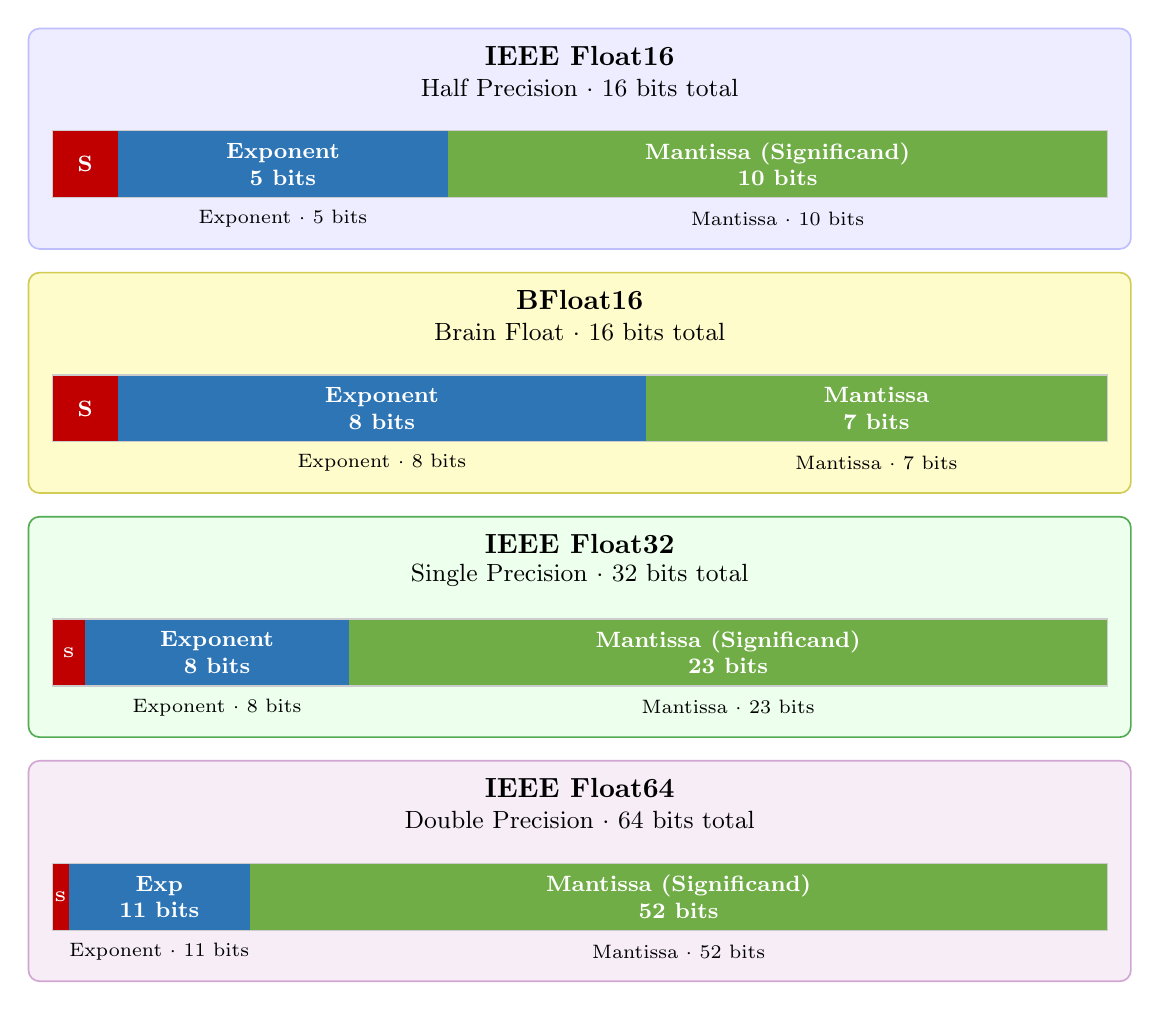
\begin{tikzpicture}[x=1cm, y=1cm]

  % ---- Color palette ----
  \definecolor{signcolor}{RGB}{192,0,0}     % red   -- sign bit
  \definecolor{expcolor} {RGB}{46,117,182}  % blue  -- exponent
  \definecolor{mancolor} {RGB}{112,173,71}  % green -- mantissa

  % ---- Panel backgrounds ----
  % Panels are 14 cm wide x 2.8 cm tall, separated by 0.3 cm gaps.
  % Y positions (bottom edge): Float16=9.30, BFloat16=6.20, Float32=3.10, Float64=0.00
  \draw[rounded corners=4pt, fill=blue!7,    draw=blue!25,        line width=0.6pt]
      (0.0,  9.30) rectangle (14.0, 12.10);  % Float16
  \draw[rounded corners=4pt, fill=yellow!20, draw=yellow!60!gray, line width=0.6pt]
      (0.0,  6.20) rectangle (14.0,  9.00);  % BFloat16
  \draw[rounded corners=4pt, fill=green!7,   draw=green!35!gray,  line width=0.6pt]
      (0.0,  3.10) rectangle (14.0,  5.90);  % Float32
  \draw[rounded corners=4pt, fill=violet!7,  draw=violet!35,      line width=0.6pt]
      (0.0,  0.00) rectangle (14.0,  2.80);  % Float64

  % ====================================================================
  % Bar geometry (shared across all panels):
  %   x range:    [0.30, 13.70]  => total bar width = 13.40 cm
  %   bar height: 0.85 cm
  %   bar bottom: panel_bottom + 0.65
  %   bar top:    panel_bottom + 1.50
  %
  % Segment x boundaries  (width = n_bits/total * 13.40):
  %   Float16  (16-bit): 0.300 | 1.138 | 5.325 | 13.700
  %   BFloat16 (16-bit): 0.300 | 1.138 | 7.838 | 13.700
  %   Float32  (32-bit): 0.300 | 0.719 | 4.069 | 13.700
  %   Float64  (64-bit): 0.300 | 0.509 | 2.813 | 13.700
  % ====================================================================

  % ------------------------------------------------------------------
  % IEEE Float16  (panel bottom y = 9.30)
  % ------------------------------------------------------------------
  \node[font=\normalsize\bfseries] at (7.0, 11.75) {IEEE Float16};
  \node[font=\small]               at (7.0, 11.35) {Half Precision $\cdot$ 16 bits total};

  % S:   1/16 * 13.40 = 0.838 cm   x: 0.300 -- 1.138,  center: 0.719
  \fill[signcolor] (0.300,  9.95) rectangle ( 1.138, 10.80);
  \node[text=white, font=\footnotesize\bfseries] at (0.719, 10.375) {S};

  % Exp: 5/16 * 13.40 = 4.188 cm   x: 1.138 -- 5.325,  center: 3.231
  \fill[expcolor]  (1.138,  9.95) rectangle ( 5.325, 10.80);
  \node[text=white, font=\footnotesize\bfseries, align=center] at (3.231, 10.375)
      {Exponent \\ 5 bits};

  % Man: 10/16 * 13.40 = 8.375 cm  x: 5.325 -- 13.700, center: 9.513
  \fill[mancolor]  (5.325,  9.95) rectangle (13.700, 10.80);
  \node[text=white, font=\footnotesize\bfseries, align=center] at (9.513, 10.375)
      {Mantissa (Significand) \\ 10 bits};

  \draw[black!20, line width=0.4pt] (0.300, 9.95) rectangle (13.700, 10.80);

  \node[font=\scriptsize] at (3.231, 9.68) {Exponent $\cdot$ 5 bits};
  \node[font=\scriptsize] at (9.513, 9.68) {Mantissa $\cdot$ 10 bits};

  % ------------------------------------------------------------------
  % BFloat16  (panel bottom y = 6.20)
  % ------------------------------------------------------------------
  \node[font=\normalsize\bfseries] at (7.0, 8.65) {BFloat16};
  \node[font=\small]               at (7.0, 8.25) {Brain Float $\cdot$ 16 bits total};

  % S:   1/16 * 13.40 = 0.838 cm   x: 0.300 -- 1.138,  center: 0.719
  \fill[signcolor] (0.300,  6.85) rectangle ( 1.138,  7.70);
  \node[text=white, font=\footnotesize\bfseries] at (0.719, 7.275) {S};

  % Exp: 8/16 * 13.40 = 6.700 cm   x: 1.138 -- 7.838,  center: 4.488
  \fill[expcolor]  (1.138,  6.85) rectangle ( 7.838,  7.70);
  \node[text=white, font=\footnotesize\bfseries, align=center] at (4.488, 7.275)
      {Exponent \\ 8 bits};

  % Man: 7/16 * 13.40 = 5.863 cm   x: 7.838 -- 13.700, center: 10.769
  \fill[mancolor]  (7.838,  6.85) rectangle (13.700,  7.70);
  \node[text=white, font=\footnotesize\bfseries, align=center] at (10.769, 7.275)
      {Mantissa \\ 7 bits};

  \draw[black!20, line width=0.4pt] (0.300, 6.85) rectangle (13.700, 7.70);

  \node[font=\scriptsize] at ( 4.488, 6.58) {Exponent $\cdot$ 8 bits};
  \node[font=\scriptsize] at (10.769, 6.58) {Mantissa $\cdot$ 7 bits};

  % ------------------------------------------------------------------
  % IEEE Float32  (panel bottom y = 3.10)
  % ------------------------------------------------------------------
  \node[font=\normalsize\bfseries] at (7.0, 5.55) {IEEE Float32};
  \node[font=\small]               at (7.0, 5.15) {Single Precision $\cdot$ 32 bits total};

  % S:   1/32 * 13.40 = 0.419 cm   x: 0.300 -- 0.719,  center: 0.510
  \fill[signcolor] (0.300,  3.75) rectangle ( 0.719,  4.60);
  \node[text=white, font=\tiny\bfseries] at (0.510, 4.175) {S};

  % Exp: 8/32 * 13.40 = 3.350 cm   x: 0.719 -- 4.069,  center: 2.394
  \fill[expcolor]  (0.719,  3.75) rectangle ( 4.069,  4.60);
  \node[text=white, font=\footnotesize\bfseries, align=center] at (2.394, 4.175)
      {Exponent \\ 8 bits};

  % Man: 23/32 * 13.40 = 9.631 cm  x: 4.069 -- 13.700, center: 8.885
  \fill[mancolor]  (4.069,  3.75) rectangle (13.700,  4.60);
  \node[text=white, font=\footnotesize\bfseries, align=center] at (8.885, 4.175)
      {Mantissa (Significand) \\ 23 bits};

  \draw[black!20, line width=0.4pt] (0.300, 3.75) rectangle (13.700, 4.60);

  \node[font=\scriptsize] at (2.394, 3.48) {Exponent $\cdot$ 8 bits};
  \node[font=\scriptsize] at (8.885, 3.48) {Mantissa $\cdot$ 23 bits};

  % ------------------------------------------------------------------
  % IEEE Float64  (panel bottom y = 0.00)
  % ------------------------------------------------------------------
  \node[font=\normalsize\bfseries] at (7.0, 2.45) {IEEE Float64};
  \node[font=\small]               at (7.0, 2.05) {Double Precision $\cdot$ 64 bits total};

  % S:    1/64 * 13.40 = 0.209 cm  x: 0.300 -- 0.509,  center: 0.405
  \fill[signcolor] (0.300,  0.65) rectangle ( 0.509,  1.50);
  \node[text=white, font=\tiny\bfseries] at (0.405, 1.075) {S};

  % Exp: 11/64 * 13.40 = 2.303 cm  x: 0.509 -- 2.813,  center: 1.661
  \fill[expcolor]  (0.509,  0.65) rectangle ( 2.813,  1.50);
  \node[text=white, font=\footnotesize\bfseries, align=center] at (1.661, 1.075)
      {Exp \\ 11 bits};

  % Man: 52/64 * 13.40 = 10.888 cm x: 2.813 -- 13.700, center: 8.257
  \fill[mancolor]  (2.813,  0.65) rectangle (13.700,  1.50);
  \node[text=white, font=\footnotesize\bfseries, align=center] at (8.257, 1.075)
      {Mantissa (Significand) \\ 52 bits};

  \draw[black!20, line width=0.4pt] (0.300, 0.65) rectangle (13.700, 1.50);

  \node[font=\scriptsize] at (1.661, 0.38) {Exponent $\cdot$ 11 bits};
  \node[font=\scriptsize] at (8.257, 0.38) {Mantissa $\cdot$ 52 bits};

\end{tikzpicture}
}
%
% \resizebox scales everything uniformly — coordinates, line widths,
% and fonts — so the result looks identical regardless of the chosen width.
%
% Recommended figure wrapper (single column):
%   \begin{figure}[t]
%     \centering
%     \resizebox{\columnwidth}{!}{% Floating-point format comparison — single-column stack layout
%
% Required in preamble:
%   \usepackage{tikz}
%
% ---- Scaling -------------------------------------------------------
% The tikzpicture is drawn at its natural size: 14 cm wide x 12.1 cm tall.
% Use \resizebox (from the graphicx package, always loaded in IEEE style)
% to scale it to whatever width you need. The height adjusts automatically.
%
%   Fit to a single text column (~8.8 cm in IEEE two-column):
%     \resizebox{\columnwidth}{!}{\input{float_formats_tikz.tex}}
%
%   Fit to the full page width (~17.8 cm in IEEE two-column):
%     \resizebox{\textwidth}{!}{\input{float_formats_tikz.tex}}
%
%   Fit to an arbitrary fraction of the column width:
%     \resizebox{0.9\columnwidth}{!}{\input{float_formats_tikz.tex}}
%
% \resizebox scales everything uniformly — coordinates, line widths,
% and fonts — so the result looks identical regardless of the chosen width.
%
% Recommended figure wrapper (single column):
%   \begin{figure}[t]
%     \centering
%     \resizebox{\columnwidth}{!}{\input{float_formats_tikz.tex}}
%     \caption{...}
%     \label{fig:float-formats}
%   \end{figure}
% --------------------------------------------------------------------
%
% Layout: 4 panels stacked vertically, each 14 cm x 2.8 cm.
% Bar widths are proportional to actual bit-field widths.
%   Float16:  S=1, Exp=5,  Man=10  (16 bits total)
%   BFloat16: S=1, Exp=8,  Man=7   (16 bits total)
%   Float32:  S=1, Exp=8,  Man=23  (32 bits total)
%   Float64:  S=1, Exp=11, Man=52  (64 bits total)

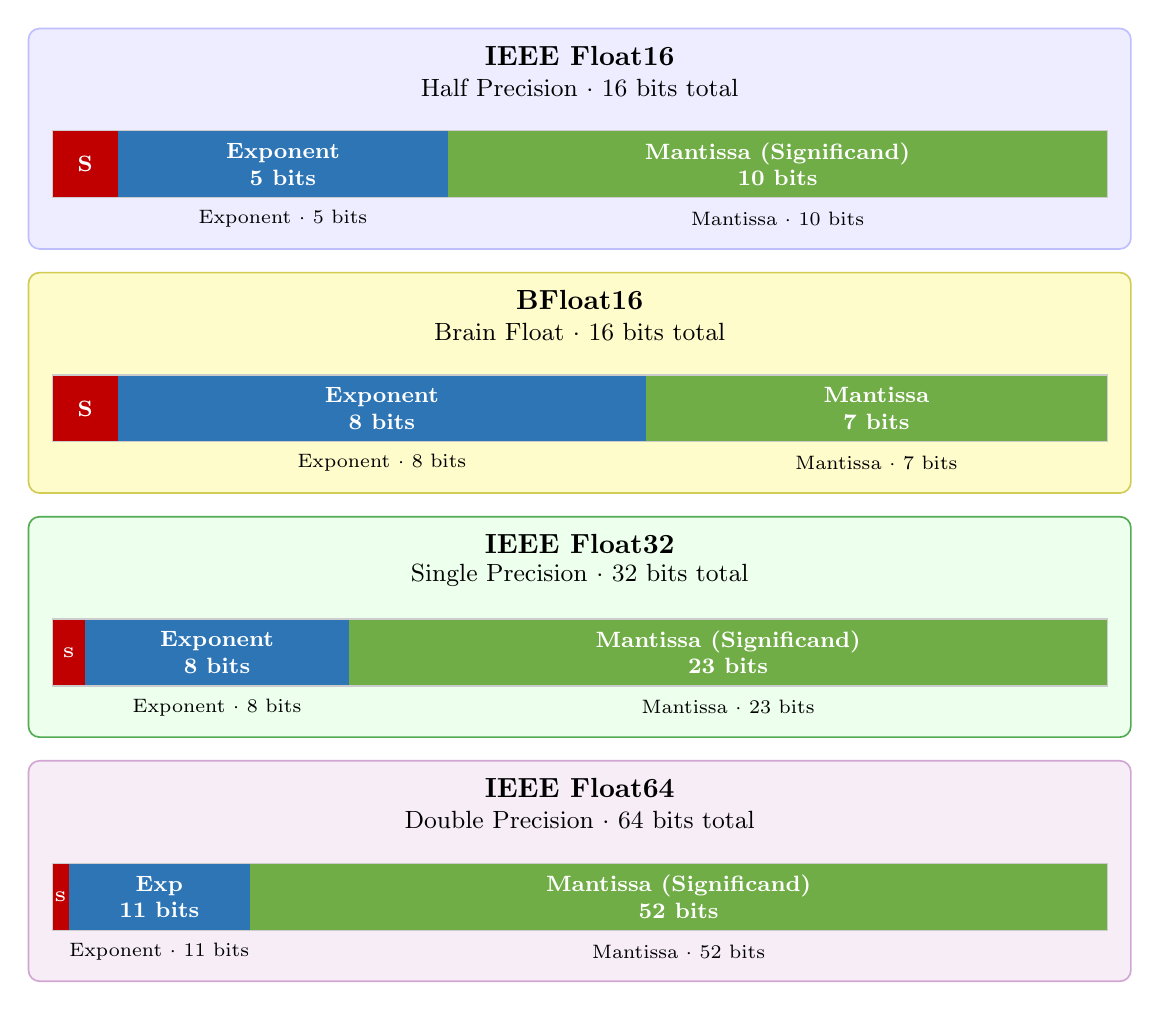
\begin{tikzpicture}[x=1cm, y=1cm]

  % ---- Color palette ----
  \definecolor{signcolor}{RGB}{192,0,0}     % red   -- sign bit
  \definecolor{expcolor} {RGB}{46,117,182}  % blue  -- exponent
  \definecolor{mancolor} {RGB}{112,173,71}  % green -- mantissa

  % ---- Panel backgrounds ----
  % Panels are 14 cm wide x 2.8 cm tall, separated by 0.3 cm gaps.
  % Y positions (bottom edge): Float16=9.30, BFloat16=6.20, Float32=3.10, Float64=0.00
  \draw[rounded corners=4pt, fill=blue!7,    draw=blue!25,        line width=0.6pt]
      (0.0,  9.30) rectangle (14.0, 12.10);  % Float16
  \draw[rounded corners=4pt, fill=yellow!20, draw=yellow!60!gray, line width=0.6pt]
      (0.0,  6.20) rectangle (14.0,  9.00);  % BFloat16
  \draw[rounded corners=4pt, fill=green!7,   draw=green!35!gray,  line width=0.6pt]
      (0.0,  3.10) rectangle (14.0,  5.90);  % Float32
  \draw[rounded corners=4pt, fill=violet!7,  draw=violet!35,      line width=0.6pt]
      (0.0,  0.00) rectangle (14.0,  2.80);  % Float64

  % ====================================================================
  % Bar geometry (shared across all panels):
  %   x range:    [0.30, 13.70]  => total bar width = 13.40 cm
  %   bar height: 0.85 cm
  %   bar bottom: panel_bottom + 0.65
  %   bar top:    panel_bottom + 1.50
  %
  % Segment x boundaries  (width = n_bits/total * 13.40):
  %   Float16  (16-bit): 0.300 | 1.138 | 5.325 | 13.700
  %   BFloat16 (16-bit): 0.300 | 1.138 | 7.838 | 13.700
  %   Float32  (32-bit): 0.300 | 0.719 | 4.069 | 13.700
  %   Float64  (64-bit): 0.300 | 0.509 | 2.813 | 13.700
  % ====================================================================

  % ------------------------------------------------------------------
  % IEEE Float16  (panel bottom y = 9.30)
  % ------------------------------------------------------------------
  \node[font=\normalsize\bfseries] at (7.0, 11.75) {IEEE Float16};
  \node[font=\small]               at (7.0, 11.35) {Half Precision $\cdot$ 16 bits total};

  % S:   1/16 * 13.40 = 0.838 cm   x: 0.300 -- 1.138,  center: 0.719
  \fill[signcolor] (0.300,  9.95) rectangle ( 1.138, 10.80);
  \node[text=white, font=\footnotesize\bfseries] at (0.719, 10.375) {S};

  % Exp: 5/16 * 13.40 = 4.188 cm   x: 1.138 -- 5.325,  center: 3.231
  \fill[expcolor]  (1.138,  9.95) rectangle ( 5.325, 10.80);
  \node[text=white, font=\footnotesize\bfseries, align=center] at (3.231, 10.375)
      {Exponent \\ 5 bits};

  % Man: 10/16 * 13.40 = 8.375 cm  x: 5.325 -- 13.700, center: 9.513
  \fill[mancolor]  (5.325,  9.95) rectangle (13.700, 10.80);
  \node[text=white, font=\footnotesize\bfseries, align=center] at (9.513, 10.375)
      {Mantissa (Significand) \\ 10 bits};

  \draw[black!20, line width=0.4pt] (0.300, 9.95) rectangle (13.700, 10.80);

  \node[font=\scriptsize] at (3.231, 9.68) {Exponent $\cdot$ 5 bits};
  \node[font=\scriptsize] at (9.513, 9.68) {Mantissa $\cdot$ 10 bits};

  % ------------------------------------------------------------------
  % BFloat16  (panel bottom y = 6.20)
  % ------------------------------------------------------------------
  \node[font=\normalsize\bfseries] at (7.0, 8.65) {BFloat16};
  \node[font=\small]               at (7.0, 8.25) {Brain Float $\cdot$ 16 bits total};

  % S:   1/16 * 13.40 = 0.838 cm   x: 0.300 -- 1.138,  center: 0.719
  \fill[signcolor] (0.300,  6.85) rectangle ( 1.138,  7.70);
  \node[text=white, font=\footnotesize\bfseries] at (0.719, 7.275) {S};

  % Exp: 8/16 * 13.40 = 6.700 cm   x: 1.138 -- 7.838,  center: 4.488
  \fill[expcolor]  (1.138,  6.85) rectangle ( 7.838,  7.70);
  \node[text=white, font=\footnotesize\bfseries, align=center] at (4.488, 7.275)
      {Exponent \\ 8 bits};

  % Man: 7/16 * 13.40 = 5.863 cm   x: 7.838 -- 13.700, center: 10.769
  \fill[mancolor]  (7.838,  6.85) rectangle (13.700,  7.70);
  \node[text=white, font=\footnotesize\bfseries, align=center] at (10.769, 7.275)
      {Mantissa \\ 7 bits};

  \draw[black!20, line width=0.4pt] (0.300, 6.85) rectangle (13.700, 7.70);

  \node[font=\scriptsize] at ( 4.488, 6.58) {Exponent $\cdot$ 8 bits};
  \node[font=\scriptsize] at (10.769, 6.58) {Mantissa $\cdot$ 7 bits};

  % ------------------------------------------------------------------
  % IEEE Float32  (panel bottom y = 3.10)
  % ------------------------------------------------------------------
  \node[font=\normalsize\bfseries] at (7.0, 5.55) {IEEE Float32};
  \node[font=\small]               at (7.0, 5.15) {Single Precision $\cdot$ 32 bits total};

  % S:   1/32 * 13.40 = 0.419 cm   x: 0.300 -- 0.719,  center: 0.510
  \fill[signcolor] (0.300,  3.75) rectangle ( 0.719,  4.60);
  \node[text=white, font=\tiny\bfseries] at (0.510, 4.175) {S};

  % Exp: 8/32 * 13.40 = 3.350 cm   x: 0.719 -- 4.069,  center: 2.394
  \fill[expcolor]  (0.719,  3.75) rectangle ( 4.069,  4.60);
  \node[text=white, font=\footnotesize\bfseries, align=center] at (2.394, 4.175)
      {Exponent \\ 8 bits};

  % Man: 23/32 * 13.40 = 9.631 cm  x: 4.069 -- 13.700, center: 8.885
  \fill[mancolor]  (4.069,  3.75) rectangle (13.700,  4.60);
  \node[text=white, font=\footnotesize\bfseries, align=center] at (8.885, 4.175)
      {Mantissa (Significand) \\ 23 bits};

  \draw[black!20, line width=0.4pt] (0.300, 3.75) rectangle (13.700, 4.60);

  \node[font=\scriptsize] at (2.394, 3.48) {Exponent $\cdot$ 8 bits};
  \node[font=\scriptsize] at (8.885, 3.48) {Mantissa $\cdot$ 23 bits};

  % ------------------------------------------------------------------
  % IEEE Float64  (panel bottom y = 0.00)
  % ------------------------------------------------------------------
  \node[font=\normalsize\bfseries] at (7.0, 2.45) {IEEE Float64};
  \node[font=\small]               at (7.0, 2.05) {Double Precision $\cdot$ 64 bits total};

  % S:    1/64 * 13.40 = 0.209 cm  x: 0.300 -- 0.509,  center: 0.405
  \fill[signcolor] (0.300,  0.65) rectangle ( 0.509,  1.50);
  \node[text=white, font=\tiny\bfseries] at (0.405, 1.075) {S};

  % Exp: 11/64 * 13.40 = 2.303 cm  x: 0.509 -- 2.813,  center: 1.661
  \fill[expcolor]  (0.509,  0.65) rectangle ( 2.813,  1.50);
  \node[text=white, font=\footnotesize\bfseries, align=center] at (1.661, 1.075)
      {Exp \\ 11 bits};

  % Man: 52/64 * 13.40 = 10.888 cm x: 2.813 -- 13.700, center: 8.257
  \fill[mancolor]  (2.813,  0.65) rectangle (13.700,  1.50);
  \node[text=white, font=\footnotesize\bfseries, align=center] at (8.257, 1.075)
      {Mantissa (Significand) \\ 52 bits};

  \draw[black!20, line width=0.4pt] (0.300, 0.65) rectangle (13.700, 1.50);

  \node[font=\scriptsize] at (1.661, 0.38) {Exponent $\cdot$ 11 bits};
  \node[font=\scriptsize] at (8.257, 0.38) {Mantissa $\cdot$ 52 bits};

\end{tikzpicture}
}
%     \caption{...}
%     \label{fig:float-formats}
%   \end{figure}
% --------------------------------------------------------------------
%
% Layout: 4 panels stacked vertically, each 14 cm x 2.8 cm.
% Bar widths are proportional to actual bit-field widths.
%   Float16:  S=1, Exp=5,  Man=10  (16 bits total)
%   BFloat16: S=1, Exp=8,  Man=7   (16 bits total)
%   Float32:  S=1, Exp=8,  Man=23  (32 bits total)
%   Float64:  S=1, Exp=11, Man=52  (64 bits total)

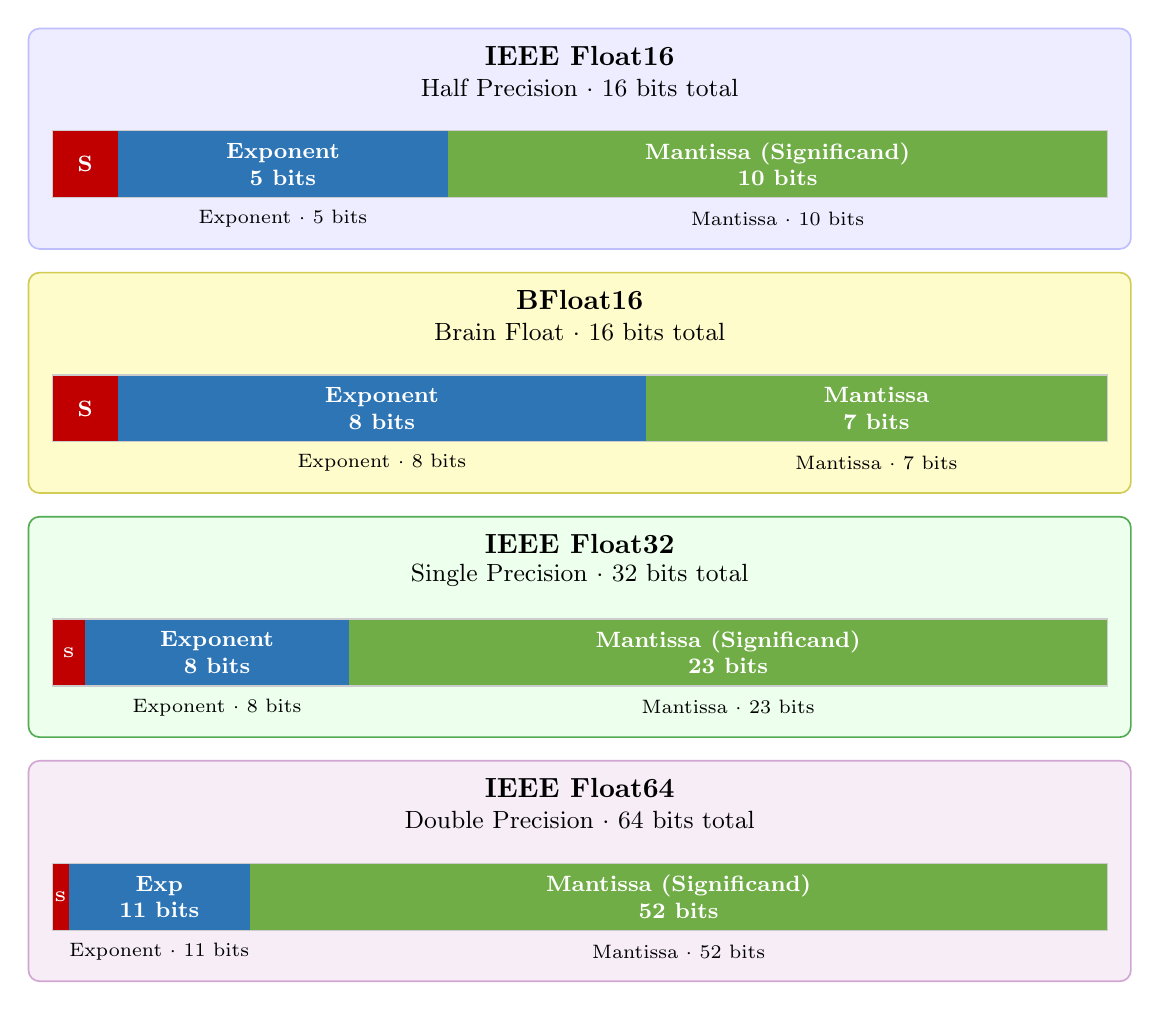
\begin{tikzpicture}[x=1cm, y=1cm]

  % ---- Color palette ----
  \definecolor{signcolor}{RGB}{192,0,0}     % red   -- sign bit
  \definecolor{expcolor} {RGB}{46,117,182}  % blue  -- exponent
  \definecolor{mancolor} {RGB}{112,173,71}  % green -- mantissa

  % ---- Panel backgrounds ----
  % Panels are 14 cm wide x 2.8 cm tall, separated by 0.3 cm gaps.
  % Y positions (bottom edge): Float16=9.30, BFloat16=6.20, Float32=3.10, Float64=0.00
  \draw[rounded corners=4pt, fill=blue!7,    draw=blue!25,        line width=0.6pt]
      (0.0,  9.30) rectangle (14.0, 12.10);  % Float16
  \draw[rounded corners=4pt, fill=yellow!20, draw=yellow!60!gray, line width=0.6pt]
      (0.0,  6.20) rectangle (14.0,  9.00);  % BFloat16
  \draw[rounded corners=4pt, fill=green!7,   draw=green!35!gray,  line width=0.6pt]
      (0.0,  3.10) rectangle (14.0,  5.90);  % Float32
  \draw[rounded corners=4pt, fill=violet!7,  draw=violet!35,      line width=0.6pt]
      (0.0,  0.00) rectangle (14.0,  2.80);  % Float64

  % ====================================================================
  % Bar geometry (shared across all panels):
  %   x range:    [0.30, 13.70]  => total bar width = 13.40 cm
  %   bar height: 0.85 cm
  %   bar bottom: panel_bottom + 0.65
  %   bar top:    panel_bottom + 1.50
  %
  % Segment x boundaries  (width = n_bits/total * 13.40):
  %   Float16  (16-bit): 0.300 | 1.138 | 5.325 | 13.700
  %   BFloat16 (16-bit): 0.300 | 1.138 | 7.838 | 13.700
  %   Float32  (32-bit): 0.300 | 0.719 | 4.069 | 13.700
  %   Float64  (64-bit): 0.300 | 0.509 | 2.813 | 13.700
  % ====================================================================

  % ------------------------------------------------------------------
  % IEEE Float16  (panel bottom y = 9.30)
  % ------------------------------------------------------------------
  \node[font=\normalsize\bfseries] at (7.0, 11.75) {IEEE Float16};
  \node[font=\small]               at (7.0, 11.35) {Half Precision $\cdot$ 16 bits total};

  % S:   1/16 * 13.40 = 0.838 cm   x: 0.300 -- 1.138,  center: 0.719
  \fill[signcolor] (0.300,  9.95) rectangle ( 1.138, 10.80);
  \node[text=white, font=\footnotesize\bfseries] at (0.719, 10.375) {S};

  % Exp: 5/16 * 13.40 = 4.188 cm   x: 1.138 -- 5.325,  center: 3.231
  \fill[expcolor]  (1.138,  9.95) rectangle ( 5.325, 10.80);
  \node[text=white, font=\footnotesize\bfseries, align=center] at (3.231, 10.375)
      {Exponent \\ 5 bits};

  % Man: 10/16 * 13.40 = 8.375 cm  x: 5.325 -- 13.700, center: 9.513
  \fill[mancolor]  (5.325,  9.95) rectangle (13.700, 10.80);
  \node[text=white, font=\footnotesize\bfseries, align=center] at (9.513, 10.375)
      {Mantissa (Significand) \\ 10 bits};

  \draw[black!20, line width=0.4pt] (0.300, 9.95) rectangle (13.700, 10.80);

  \node[font=\scriptsize] at (3.231, 9.68) {Exponent $\cdot$ 5 bits};
  \node[font=\scriptsize] at (9.513, 9.68) {Mantissa $\cdot$ 10 bits};

  % ------------------------------------------------------------------
  % BFloat16  (panel bottom y = 6.20)
  % ------------------------------------------------------------------
  \node[font=\normalsize\bfseries] at (7.0, 8.65) {BFloat16};
  \node[font=\small]               at (7.0, 8.25) {Brain Float $\cdot$ 16 bits total};

  % S:   1/16 * 13.40 = 0.838 cm   x: 0.300 -- 1.138,  center: 0.719
  \fill[signcolor] (0.300,  6.85) rectangle ( 1.138,  7.70);
  \node[text=white, font=\footnotesize\bfseries] at (0.719, 7.275) {S};

  % Exp: 8/16 * 13.40 = 6.700 cm   x: 1.138 -- 7.838,  center: 4.488
  \fill[expcolor]  (1.138,  6.85) rectangle ( 7.838,  7.70);
  \node[text=white, font=\footnotesize\bfseries, align=center] at (4.488, 7.275)
      {Exponent \\ 8 bits};

  % Man: 7/16 * 13.40 = 5.863 cm   x: 7.838 -- 13.700, center: 10.769
  \fill[mancolor]  (7.838,  6.85) rectangle (13.700,  7.70);
  \node[text=white, font=\footnotesize\bfseries, align=center] at (10.769, 7.275)
      {Mantissa \\ 7 bits};

  \draw[black!20, line width=0.4pt] (0.300, 6.85) rectangle (13.700, 7.70);

  \node[font=\scriptsize] at ( 4.488, 6.58) {Exponent $\cdot$ 8 bits};
  \node[font=\scriptsize] at (10.769, 6.58) {Mantissa $\cdot$ 7 bits};

  % ------------------------------------------------------------------
  % IEEE Float32  (panel bottom y = 3.10)
  % ------------------------------------------------------------------
  \node[font=\normalsize\bfseries] at (7.0, 5.55) {IEEE Float32};
  \node[font=\small]               at (7.0, 5.15) {Single Precision $\cdot$ 32 bits total};

  % S:   1/32 * 13.40 = 0.419 cm   x: 0.300 -- 0.719,  center: 0.510
  \fill[signcolor] (0.300,  3.75) rectangle ( 0.719,  4.60);
  \node[text=white, font=\tiny\bfseries] at (0.510, 4.175) {S};

  % Exp: 8/32 * 13.40 = 3.350 cm   x: 0.719 -- 4.069,  center: 2.394
  \fill[expcolor]  (0.719,  3.75) rectangle ( 4.069,  4.60);
  \node[text=white, font=\footnotesize\bfseries, align=center] at (2.394, 4.175)
      {Exponent \\ 8 bits};

  % Man: 23/32 * 13.40 = 9.631 cm  x: 4.069 -- 13.700, center: 8.885
  \fill[mancolor]  (4.069,  3.75) rectangle (13.700,  4.60);
  \node[text=white, font=\footnotesize\bfseries, align=center] at (8.885, 4.175)
      {Mantissa (Significand) \\ 23 bits};

  \draw[black!20, line width=0.4pt] (0.300, 3.75) rectangle (13.700, 4.60);

  \node[font=\scriptsize] at (2.394, 3.48) {Exponent $\cdot$ 8 bits};
  \node[font=\scriptsize] at (8.885, 3.48) {Mantissa $\cdot$ 23 bits};

  % ------------------------------------------------------------------
  % IEEE Float64  (panel bottom y = 0.00)
  % ------------------------------------------------------------------
  \node[font=\normalsize\bfseries] at (7.0, 2.45) {IEEE Float64};
  \node[font=\small]               at (7.0, 2.05) {Double Precision $\cdot$ 64 bits total};

  % S:    1/64 * 13.40 = 0.209 cm  x: 0.300 -- 0.509,  center: 0.405
  \fill[signcolor] (0.300,  0.65) rectangle ( 0.509,  1.50);
  \node[text=white, font=\tiny\bfseries] at (0.405, 1.075) {S};

  % Exp: 11/64 * 13.40 = 2.303 cm  x: 0.509 -- 2.813,  center: 1.661
  \fill[expcolor]  (0.509,  0.65) rectangle ( 2.813,  1.50);
  \node[text=white, font=\footnotesize\bfseries, align=center] at (1.661, 1.075)
      {Exp \\ 11 bits};

  % Man: 52/64 * 13.40 = 10.888 cm x: 2.813 -- 13.700, center: 8.257
  \fill[mancolor]  (2.813,  0.65) rectangle (13.700,  1.50);
  \node[text=white, font=\footnotesize\bfseries, align=center] at (8.257, 1.075)
      {Mantissa (Significand) \\ 52 bits};

  \draw[black!20, line width=0.4pt] (0.300, 0.65) rectangle (13.700, 1.50);

  \node[font=\scriptsize] at (1.661, 0.38) {Exponent $\cdot$ 11 bits};
  \node[font=\scriptsize] at (8.257, 0.38) {Mantissa $\cdot$ 52 bits};

\end{tikzpicture}
}
%
% \resizebox scales everything uniformly — coordinates, line widths,
% and fonts — so the result looks identical regardless of the chosen width.
%
% Recommended figure wrapper (single column):
%   \begin{figure}[t]
%     \centering
%     \resizebox{\columnwidth}{!}{% Floating-point format comparison — single-column stack layout
%
% Required in preamble:
%   \usepackage{tikz}
%
% ---- Scaling -------------------------------------------------------
% The tikzpicture is drawn at its natural size: 14 cm wide x 12.1 cm tall.
% Use \resizebox (from the graphicx package, always loaded in IEEE style)
% to scale it to whatever width you need. The height adjusts automatically.
%
%   Fit to a single text column (~8.8 cm in IEEE two-column):
%     \resizebox{\columnwidth}{!}{% Floating-point format comparison — single-column stack layout
%
% Required in preamble:
%   \usepackage{tikz}
%
% ---- Scaling -------------------------------------------------------
% The tikzpicture is drawn at its natural size: 14 cm wide x 12.1 cm tall.
% Use \resizebox (from the graphicx package, always loaded in IEEE style)
% to scale it to whatever width you need. The height adjusts automatically.
%
%   Fit to a single text column (~8.8 cm in IEEE two-column):
%     \resizebox{\columnwidth}{!}{\input{float_formats_tikz.tex}}
%
%   Fit to the full page width (~17.8 cm in IEEE two-column):
%     \resizebox{\textwidth}{!}{\input{float_formats_tikz.tex}}
%
%   Fit to an arbitrary fraction of the column width:
%     \resizebox{0.9\columnwidth}{!}{\input{float_formats_tikz.tex}}
%
% \resizebox scales everything uniformly — coordinates, line widths,
% and fonts — so the result looks identical regardless of the chosen width.
%
% Recommended figure wrapper (single column):
%   \begin{figure}[t]
%     \centering
%     \resizebox{\columnwidth}{!}{\input{float_formats_tikz.tex}}
%     \caption{...}
%     \label{fig:float-formats}
%   \end{figure}
% --------------------------------------------------------------------
%
% Layout: 4 panels stacked vertically, each 14 cm x 2.8 cm.
% Bar widths are proportional to actual bit-field widths.
%   Float16:  S=1, Exp=5,  Man=10  (16 bits total)
%   BFloat16: S=1, Exp=8,  Man=7   (16 bits total)
%   Float32:  S=1, Exp=8,  Man=23  (32 bits total)
%   Float64:  S=1, Exp=11, Man=52  (64 bits total)

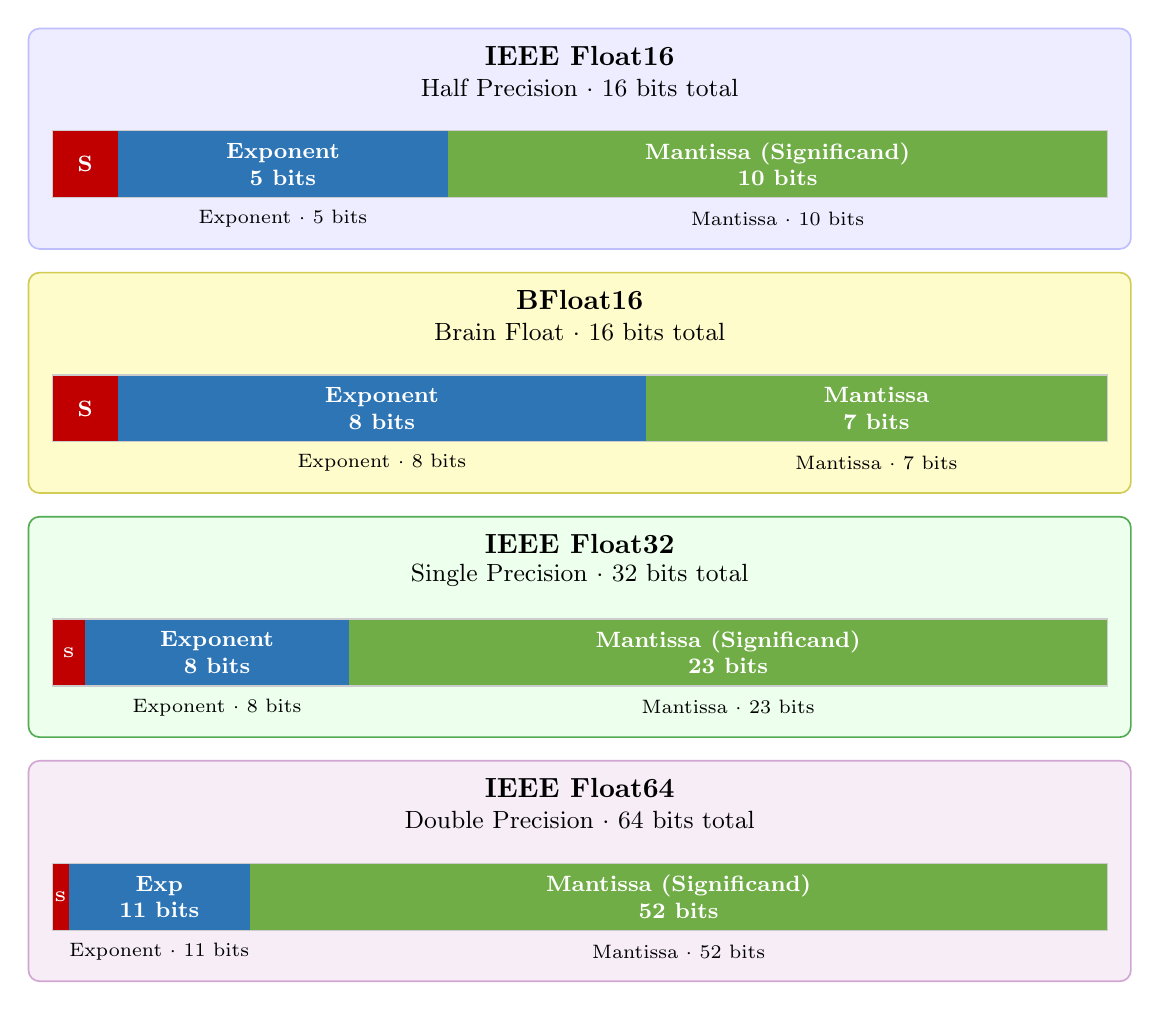
\begin{tikzpicture}[x=1cm, y=1cm]

  % ---- Color palette ----
  \definecolor{signcolor}{RGB}{192,0,0}     % red   -- sign bit
  \definecolor{expcolor} {RGB}{46,117,182}  % blue  -- exponent
  \definecolor{mancolor} {RGB}{112,173,71}  % green -- mantissa

  % ---- Panel backgrounds ----
  % Panels are 14 cm wide x 2.8 cm tall, separated by 0.3 cm gaps.
  % Y positions (bottom edge): Float16=9.30, BFloat16=6.20, Float32=3.10, Float64=0.00
  \draw[rounded corners=4pt, fill=blue!7,    draw=blue!25,        line width=0.6pt]
      (0.0,  9.30) rectangle (14.0, 12.10);  % Float16
  \draw[rounded corners=4pt, fill=yellow!20, draw=yellow!60!gray, line width=0.6pt]
      (0.0,  6.20) rectangle (14.0,  9.00);  % BFloat16
  \draw[rounded corners=4pt, fill=green!7,   draw=green!35!gray,  line width=0.6pt]
      (0.0,  3.10) rectangle (14.0,  5.90);  % Float32
  \draw[rounded corners=4pt, fill=violet!7,  draw=violet!35,      line width=0.6pt]
      (0.0,  0.00) rectangle (14.0,  2.80);  % Float64

  % ====================================================================
  % Bar geometry (shared across all panels):
  %   x range:    [0.30, 13.70]  => total bar width = 13.40 cm
  %   bar height: 0.85 cm
  %   bar bottom: panel_bottom + 0.65
  %   bar top:    panel_bottom + 1.50
  %
  % Segment x boundaries  (width = n_bits/total * 13.40):
  %   Float16  (16-bit): 0.300 | 1.138 | 5.325 | 13.700
  %   BFloat16 (16-bit): 0.300 | 1.138 | 7.838 | 13.700
  %   Float32  (32-bit): 0.300 | 0.719 | 4.069 | 13.700
  %   Float64  (64-bit): 0.300 | 0.509 | 2.813 | 13.700
  % ====================================================================

  % ------------------------------------------------------------------
  % IEEE Float16  (panel bottom y = 9.30)
  % ------------------------------------------------------------------
  \node[font=\normalsize\bfseries] at (7.0, 11.75) {IEEE Float16};
  \node[font=\small]               at (7.0, 11.35) {Half Precision $\cdot$ 16 bits total};

  % S:   1/16 * 13.40 = 0.838 cm   x: 0.300 -- 1.138,  center: 0.719
  \fill[signcolor] (0.300,  9.95) rectangle ( 1.138, 10.80);
  \node[text=white, font=\footnotesize\bfseries] at (0.719, 10.375) {S};

  % Exp: 5/16 * 13.40 = 4.188 cm   x: 1.138 -- 5.325,  center: 3.231
  \fill[expcolor]  (1.138,  9.95) rectangle ( 5.325, 10.80);
  \node[text=white, font=\footnotesize\bfseries, align=center] at (3.231, 10.375)
      {Exponent \\ 5 bits};

  % Man: 10/16 * 13.40 = 8.375 cm  x: 5.325 -- 13.700, center: 9.513
  \fill[mancolor]  (5.325,  9.95) rectangle (13.700, 10.80);
  \node[text=white, font=\footnotesize\bfseries, align=center] at (9.513, 10.375)
      {Mantissa (Significand) \\ 10 bits};

  \draw[black!20, line width=0.4pt] (0.300, 9.95) rectangle (13.700, 10.80);

  \node[font=\scriptsize] at (3.231, 9.68) {Exponent $\cdot$ 5 bits};
  \node[font=\scriptsize] at (9.513, 9.68) {Mantissa $\cdot$ 10 bits};

  % ------------------------------------------------------------------
  % BFloat16  (panel bottom y = 6.20)
  % ------------------------------------------------------------------
  \node[font=\normalsize\bfseries] at (7.0, 8.65) {BFloat16};
  \node[font=\small]               at (7.0, 8.25) {Brain Float $\cdot$ 16 bits total};

  % S:   1/16 * 13.40 = 0.838 cm   x: 0.300 -- 1.138,  center: 0.719
  \fill[signcolor] (0.300,  6.85) rectangle ( 1.138,  7.70);
  \node[text=white, font=\footnotesize\bfseries] at (0.719, 7.275) {S};

  % Exp: 8/16 * 13.40 = 6.700 cm   x: 1.138 -- 7.838,  center: 4.488
  \fill[expcolor]  (1.138,  6.85) rectangle ( 7.838,  7.70);
  \node[text=white, font=\footnotesize\bfseries, align=center] at (4.488, 7.275)
      {Exponent \\ 8 bits};

  % Man: 7/16 * 13.40 = 5.863 cm   x: 7.838 -- 13.700, center: 10.769
  \fill[mancolor]  (7.838,  6.85) rectangle (13.700,  7.70);
  \node[text=white, font=\footnotesize\bfseries, align=center] at (10.769, 7.275)
      {Mantissa \\ 7 bits};

  \draw[black!20, line width=0.4pt] (0.300, 6.85) rectangle (13.700, 7.70);

  \node[font=\scriptsize] at ( 4.488, 6.58) {Exponent $\cdot$ 8 bits};
  \node[font=\scriptsize] at (10.769, 6.58) {Mantissa $\cdot$ 7 bits};

  % ------------------------------------------------------------------
  % IEEE Float32  (panel bottom y = 3.10)
  % ------------------------------------------------------------------
  \node[font=\normalsize\bfseries] at (7.0, 5.55) {IEEE Float32};
  \node[font=\small]               at (7.0, 5.15) {Single Precision $\cdot$ 32 bits total};

  % S:   1/32 * 13.40 = 0.419 cm   x: 0.300 -- 0.719,  center: 0.510
  \fill[signcolor] (0.300,  3.75) rectangle ( 0.719,  4.60);
  \node[text=white, font=\tiny\bfseries] at (0.510, 4.175) {S};

  % Exp: 8/32 * 13.40 = 3.350 cm   x: 0.719 -- 4.069,  center: 2.394
  \fill[expcolor]  (0.719,  3.75) rectangle ( 4.069,  4.60);
  \node[text=white, font=\footnotesize\bfseries, align=center] at (2.394, 4.175)
      {Exponent \\ 8 bits};

  % Man: 23/32 * 13.40 = 9.631 cm  x: 4.069 -- 13.700, center: 8.885
  \fill[mancolor]  (4.069,  3.75) rectangle (13.700,  4.60);
  \node[text=white, font=\footnotesize\bfseries, align=center] at (8.885, 4.175)
      {Mantissa (Significand) \\ 23 bits};

  \draw[black!20, line width=0.4pt] (0.300, 3.75) rectangle (13.700, 4.60);

  \node[font=\scriptsize] at (2.394, 3.48) {Exponent $\cdot$ 8 bits};
  \node[font=\scriptsize] at (8.885, 3.48) {Mantissa $\cdot$ 23 bits};

  % ------------------------------------------------------------------
  % IEEE Float64  (panel bottom y = 0.00)
  % ------------------------------------------------------------------
  \node[font=\normalsize\bfseries] at (7.0, 2.45) {IEEE Float64};
  \node[font=\small]               at (7.0, 2.05) {Double Precision $\cdot$ 64 bits total};

  % S:    1/64 * 13.40 = 0.209 cm  x: 0.300 -- 0.509,  center: 0.405
  \fill[signcolor] (0.300,  0.65) rectangle ( 0.509,  1.50);
  \node[text=white, font=\tiny\bfseries] at (0.405, 1.075) {S};

  % Exp: 11/64 * 13.40 = 2.303 cm  x: 0.509 -- 2.813,  center: 1.661
  \fill[expcolor]  (0.509,  0.65) rectangle ( 2.813,  1.50);
  \node[text=white, font=\footnotesize\bfseries, align=center] at (1.661, 1.075)
      {Exp \\ 11 bits};

  % Man: 52/64 * 13.40 = 10.888 cm x: 2.813 -- 13.700, center: 8.257
  \fill[mancolor]  (2.813,  0.65) rectangle (13.700,  1.50);
  \node[text=white, font=\footnotesize\bfseries, align=center] at (8.257, 1.075)
      {Mantissa (Significand) \\ 52 bits};

  \draw[black!20, line width=0.4pt] (0.300, 0.65) rectangle (13.700, 1.50);

  \node[font=\scriptsize] at (1.661, 0.38) {Exponent $\cdot$ 11 bits};
  \node[font=\scriptsize] at (8.257, 0.38) {Mantissa $\cdot$ 52 bits};

\end{tikzpicture}
}
%
%   Fit to the full page width (~17.8 cm in IEEE two-column):
%     \resizebox{\textwidth}{!}{% Floating-point format comparison — single-column stack layout
%
% Required in preamble:
%   \usepackage{tikz}
%
% ---- Scaling -------------------------------------------------------
% The tikzpicture is drawn at its natural size: 14 cm wide x 12.1 cm tall.
% Use \resizebox (from the graphicx package, always loaded in IEEE style)
% to scale it to whatever width you need. The height adjusts automatically.
%
%   Fit to a single text column (~8.8 cm in IEEE two-column):
%     \resizebox{\columnwidth}{!}{\input{float_formats_tikz.tex}}
%
%   Fit to the full page width (~17.8 cm in IEEE two-column):
%     \resizebox{\textwidth}{!}{\input{float_formats_tikz.tex}}
%
%   Fit to an arbitrary fraction of the column width:
%     \resizebox{0.9\columnwidth}{!}{\input{float_formats_tikz.tex}}
%
% \resizebox scales everything uniformly — coordinates, line widths,
% and fonts — so the result looks identical regardless of the chosen width.
%
% Recommended figure wrapper (single column):
%   \begin{figure}[t]
%     \centering
%     \resizebox{\columnwidth}{!}{\input{float_formats_tikz.tex}}
%     \caption{...}
%     \label{fig:float-formats}
%   \end{figure}
% --------------------------------------------------------------------
%
% Layout: 4 panels stacked vertically, each 14 cm x 2.8 cm.
% Bar widths are proportional to actual bit-field widths.
%   Float16:  S=1, Exp=5,  Man=10  (16 bits total)
%   BFloat16: S=1, Exp=8,  Man=7   (16 bits total)
%   Float32:  S=1, Exp=8,  Man=23  (32 bits total)
%   Float64:  S=1, Exp=11, Man=52  (64 bits total)

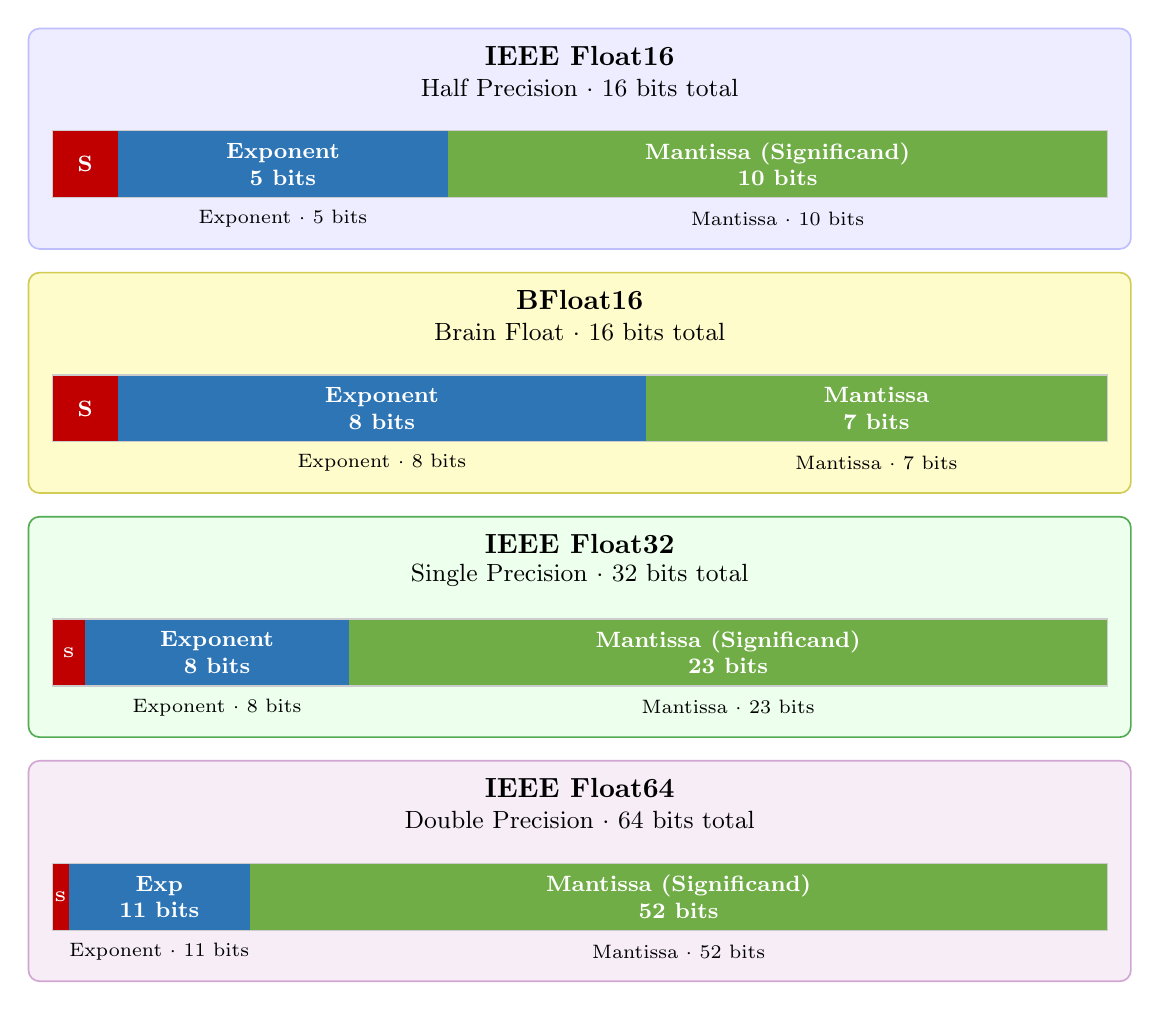
\begin{tikzpicture}[x=1cm, y=1cm]

  % ---- Color palette ----
  \definecolor{signcolor}{RGB}{192,0,0}     % red   -- sign bit
  \definecolor{expcolor} {RGB}{46,117,182}  % blue  -- exponent
  \definecolor{mancolor} {RGB}{112,173,71}  % green -- mantissa

  % ---- Panel backgrounds ----
  % Panels are 14 cm wide x 2.8 cm tall, separated by 0.3 cm gaps.
  % Y positions (bottom edge): Float16=9.30, BFloat16=6.20, Float32=3.10, Float64=0.00
  \draw[rounded corners=4pt, fill=blue!7,    draw=blue!25,        line width=0.6pt]
      (0.0,  9.30) rectangle (14.0, 12.10);  % Float16
  \draw[rounded corners=4pt, fill=yellow!20, draw=yellow!60!gray, line width=0.6pt]
      (0.0,  6.20) rectangle (14.0,  9.00);  % BFloat16
  \draw[rounded corners=4pt, fill=green!7,   draw=green!35!gray,  line width=0.6pt]
      (0.0,  3.10) rectangle (14.0,  5.90);  % Float32
  \draw[rounded corners=4pt, fill=violet!7,  draw=violet!35,      line width=0.6pt]
      (0.0,  0.00) rectangle (14.0,  2.80);  % Float64

  % ====================================================================
  % Bar geometry (shared across all panels):
  %   x range:    [0.30, 13.70]  => total bar width = 13.40 cm
  %   bar height: 0.85 cm
  %   bar bottom: panel_bottom + 0.65
  %   bar top:    panel_bottom + 1.50
  %
  % Segment x boundaries  (width = n_bits/total * 13.40):
  %   Float16  (16-bit): 0.300 | 1.138 | 5.325 | 13.700
  %   BFloat16 (16-bit): 0.300 | 1.138 | 7.838 | 13.700
  %   Float32  (32-bit): 0.300 | 0.719 | 4.069 | 13.700
  %   Float64  (64-bit): 0.300 | 0.509 | 2.813 | 13.700
  % ====================================================================

  % ------------------------------------------------------------------
  % IEEE Float16  (panel bottom y = 9.30)
  % ------------------------------------------------------------------
  \node[font=\normalsize\bfseries] at (7.0, 11.75) {IEEE Float16};
  \node[font=\small]               at (7.0, 11.35) {Half Precision $\cdot$ 16 bits total};

  % S:   1/16 * 13.40 = 0.838 cm   x: 0.300 -- 1.138,  center: 0.719
  \fill[signcolor] (0.300,  9.95) rectangle ( 1.138, 10.80);
  \node[text=white, font=\footnotesize\bfseries] at (0.719, 10.375) {S};

  % Exp: 5/16 * 13.40 = 4.188 cm   x: 1.138 -- 5.325,  center: 3.231
  \fill[expcolor]  (1.138,  9.95) rectangle ( 5.325, 10.80);
  \node[text=white, font=\footnotesize\bfseries, align=center] at (3.231, 10.375)
      {Exponent \\ 5 bits};

  % Man: 10/16 * 13.40 = 8.375 cm  x: 5.325 -- 13.700, center: 9.513
  \fill[mancolor]  (5.325,  9.95) rectangle (13.700, 10.80);
  \node[text=white, font=\footnotesize\bfseries, align=center] at (9.513, 10.375)
      {Mantissa (Significand) \\ 10 bits};

  \draw[black!20, line width=0.4pt] (0.300, 9.95) rectangle (13.700, 10.80);

  \node[font=\scriptsize] at (3.231, 9.68) {Exponent $\cdot$ 5 bits};
  \node[font=\scriptsize] at (9.513, 9.68) {Mantissa $\cdot$ 10 bits};

  % ------------------------------------------------------------------
  % BFloat16  (panel bottom y = 6.20)
  % ------------------------------------------------------------------
  \node[font=\normalsize\bfseries] at (7.0, 8.65) {BFloat16};
  \node[font=\small]               at (7.0, 8.25) {Brain Float $\cdot$ 16 bits total};

  % S:   1/16 * 13.40 = 0.838 cm   x: 0.300 -- 1.138,  center: 0.719
  \fill[signcolor] (0.300,  6.85) rectangle ( 1.138,  7.70);
  \node[text=white, font=\footnotesize\bfseries] at (0.719, 7.275) {S};

  % Exp: 8/16 * 13.40 = 6.700 cm   x: 1.138 -- 7.838,  center: 4.488
  \fill[expcolor]  (1.138,  6.85) rectangle ( 7.838,  7.70);
  \node[text=white, font=\footnotesize\bfseries, align=center] at (4.488, 7.275)
      {Exponent \\ 8 bits};

  % Man: 7/16 * 13.40 = 5.863 cm   x: 7.838 -- 13.700, center: 10.769
  \fill[mancolor]  (7.838,  6.85) rectangle (13.700,  7.70);
  \node[text=white, font=\footnotesize\bfseries, align=center] at (10.769, 7.275)
      {Mantissa \\ 7 bits};

  \draw[black!20, line width=0.4pt] (0.300, 6.85) rectangle (13.700, 7.70);

  \node[font=\scriptsize] at ( 4.488, 6.58) {Exponent $\cdot$ 8 bits};
  \node[font=\scriptsize] at (10.769, 6.58) {Mantissa $\cdot$ 7 bits};

  % ------------------------------------------------------------------
  % IEEE Float32  (panel bottom y = 3.10)
  % ------------------------------------------------------------------
  \node[font=\normalsize\bfseries] at (7.0, 5.55) {IEEE Float32};
  \node[font=\small]               at (7.0, 5.15) {Single Precision $\cdot$ 32 bits total};

  % S:   1/32 * 13.40 = 0.419 cm   x: 0.300 -- 0.719,  center: 0.510
  \fill[signcolor] (0.300,  3.75) rectangle ( 0.719,  4.60);
  \node[text=white, font=\tiny\bfseries] at (0.510, 4.175) {S};

  % Exp: 8/32 * 13.40 = 3.350 cm   x: 0.719 -- 4.069,  center: 2.394
  \fill[expcolor]  (0.719,  3.75) rectangle ( 4.069,  4.60);
  \node[text=white, font=\footnotesize\bfseries, align=center] at (2.394, 4.175)
      {Exponent \\ 8 bits};

  % Man: 23/32 * 13.40 = 9.631 cm  x: 4.069 -- 13.700, center: 8.885
  \fill[mancolor]  (4.069,  3.75) rectangle (13.700,  4.60);
  \node[text=white, font=\footnotesize\bfseries, align=center] at (8.885, 4.175)
      {Mantissa (Significand) \\ 23 bits};

  \draw[black!20, line width=0.4pt] (0.300, 3.75) rectangle (13.700, 4.60);

  \node[font=\scriptsize] at (2.394, 3.48) {Exponent $\cdot$ 8 bits};
  \node[font=\scriptsize] at (8.885, 3.48) {Mantissa $\cdot$ 23 bits};

  % ------------------------------------------------------------------
  % IEEE Float64  (panel bottom y = 0.00)
  % ------------------------------------------------------------------
  \node[font=\normalsize\bfseries] at (7.0, 2.45) {IEEE Float64};
  \node[font=\small]               at (7.0, 2.05) {Double Precision $\cdot$ 64 bits total};

  % S:    1/64 * 13.40 = 0.209 cm  x: 0.300 -- 0.509,  center: 0.405
  \fill[signcolor] (0.300,  0.65) rectangle ( 0.509,  1.50);
  \node[text=white, font=\tiny\bfseries] at (0.405, 1.075) {S};

  % Exp: 11/64 * 13.40 = 2.303 cm  x: 0.509 -- 2.813,  center: 1.661
  \fill[expcolor]  (0.509,  0.65) rectangle ( 2.813,  1.50);
  \node[text=white, font=\footnotesize\bfseries, align=center] at (1.661, 1.075)
      {Exp \\ 11 bits};

  % Man: 52/64 * 13.40 = 10.888 cm x: 2.813 -- 13.700, center: 8.257
  \fill[mancolor]  (2.813,  0.65) rectangle (13.700,  1.50);
  \node[text=white, font=\footnotesize\bfseries, align=center] at (8.257, 1.075)
      {Mantissa (Significand) \\ 52 bits};

  \draw[black!20, line width=0.4pt] (0.300, 0.65) rectangle (13.700, 1.50);

  \node[font=\scriptsize] at (1.661, 0.38) {Exponent $\cdot$ 11 bits};
  \node[font=\scriptsize] at (8.257, 0.38) {Mantissa $\cdot$ 52 bits};

\end{tikzpicture}
}
%
%   Fit to an arbitrary fraction of the column width:
%     \resizebox{0.9\columnwidth}{!}{% Floating-point format comparison — single-column stack layout
%
% Required in preamble:
%   \usepackage{tikz}
%
% ---- Scaling -------------------------------------------------------
% The tikzpicture is drawn at its natural size: 14 cm wide x 12.1 cm tall.
% Use \resizebox (from the graphicx package, always loaded in IEEE style)
% to scale it to whatever width you need. The height adjusts automatically.
%
%   Fit to a single text column (~8.8 cm in IEEE two-column):
%     \resizebox{\columnwidth}{!}{\input{float_formats_tikz.tex}}
%
%   Fit to the full page width (~17.8 cm in IEEE two-column):
%     \resizebox{\textwidth}{!}{\input{float_formats_tikz.tex}}
%
%   Fit to an arbitrary fraction of the column width:
%     \resizebox{0.9\columnwidth}{!}{\input{float_formats_tikz.tex}}
%
% \resizebox scales everything uniformly — coordinates, line widths,
% and fonts — so the result looks identical regardless of the chosen width.
%
% Recommended figure wrapper (single column):
%   \begin{figure}[t]
%     \centering
%     \resizebox{\columnwidth}{!}{\input{float_formats_tikz.tex}}
%     \caption{...}
%     \label{fig:float-formats}
%   \end{figure}
% --------------------------------------------------------------------
%
% Layout: 4 panels stacked vertically, each 14 cm x 2.8 cm.
% Bar widths are proportional to actual bit-field widths.
%   Float16:  S=1, Exp=5,  Man=10  (16 bits total)
%   BFloat16: S=1, Exp=8,  Man=7   (16 bits total)
%   Float32:  S=1, Exp=8,  Man=23  (32 bits total)
%   Float64:  S=1, Exp=11, Man=52  (64 bits total)

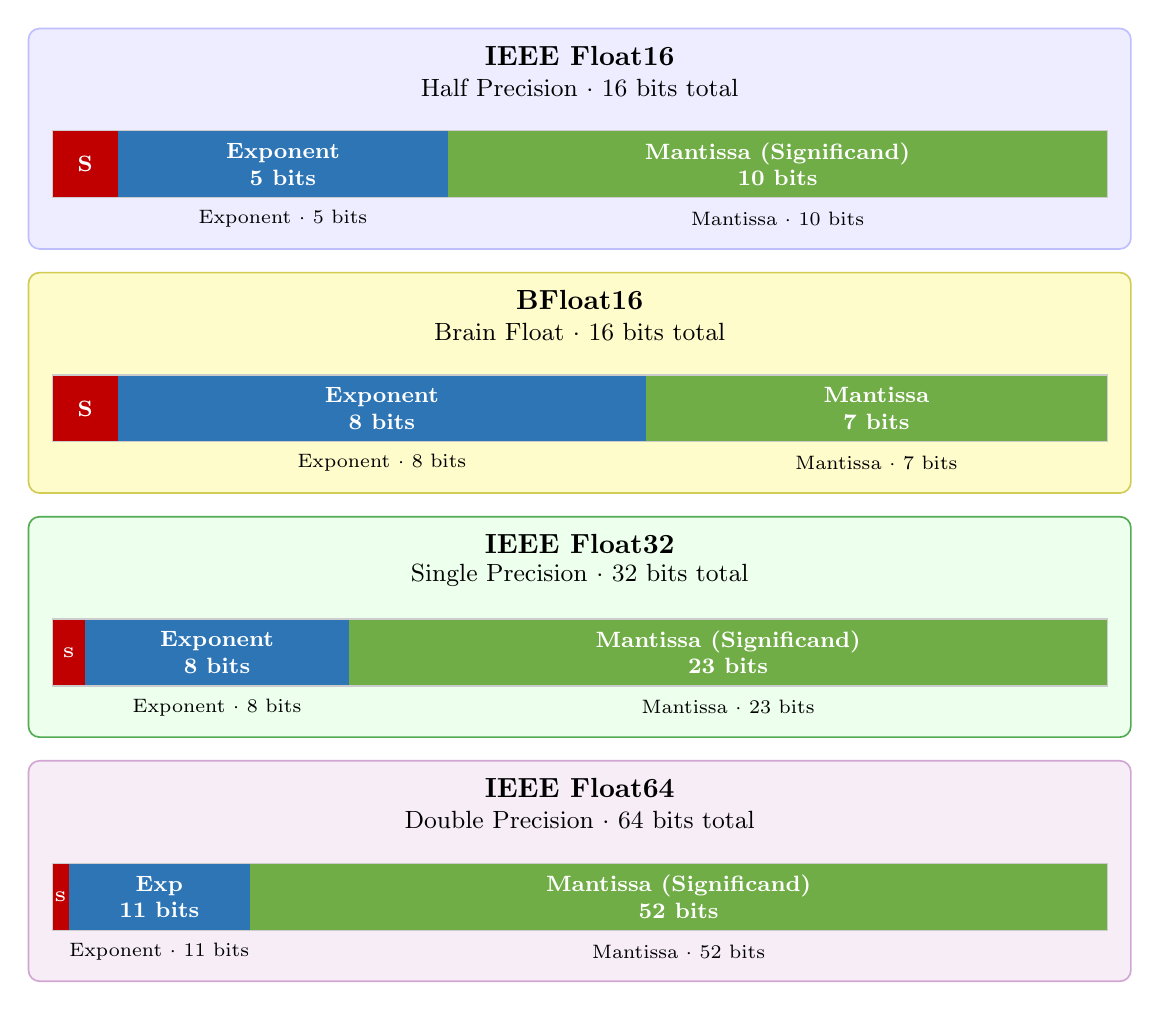
\begin{tikzpicture}[x=1cm, y=1cm]

  % ---- Color palette ----
  \definecolor{signcolor}{RGB}{192,0,0}     % red   -- sign bit
  \definecolor{expcolor} {RGB}{46,117,182}  % blue  -- exponent
  \definecolor{mancolor} {RGB}{112,173,71}  % green -- mantissa

  % ---- Panel backgrounds ----
  % Panels are 14 cm wide x 2.8 cm tall, separated by 0.3 cm gaps.
  % Y positions (bottom edge): Float16=9.30, BFloat16=6.20, Float32=3.10, Float64=0.00
  \draw[rounded corners=4pt, fill=blue!7,    draw=blue!25,        line width=0.6pt]
      (0.0,  9.30) rectangle (14.0, 12.10);  % Float16
  \draw[rounded corners=4pt, fill=yellow!20, draw=yellow!60!gray, line width=0.6pt]
      (0.0,  6.20) rectangle (14.0,  9.00);  % BFloat16
  \draw[rounded corners=4pt, fill=green!7,   draw=green!35!gray,  line width=0.6pt]
      (0.0,  3.10) rectangle (14.0,  5.90);  % Float32
  \draw[rounded corners=4pt, fill=violet!7,  draw=violet!35,      line width=0.6pt]
      (0.0,  0.00) rectangle (14.0,  2.80);  % Float64

  % ====================================================================
  % Bar geometry (shared across all panels):
  %   x range:    [0.30, 13.70]  => total bar width = 13.40 cm
  %   bar height: 0.85 cm
  %   bar bottom: panel_bottom + 0.65
  %   bar top:    panel_bottom + 1.50
  %
  % Segment x boundaries  (width = n_bits/total * 13.40):
  %   Float16  (16-bit): 0.300 | 1.138 | 5.325 | 13.700
  %   BFloat16 (16-bit): 0.300 | 1.138 | 7.838 | 13.700
  %   Float32  (32-bit): 0.300 | 0.719 | 4.069 | 13.700
  %   Float64  (64-bit): 0.300 | 0.509 | 2.813 | 13.700
  % ====================================================================

  % ------------------------------------------------------------------
  % IEEE Float16  (panel bottom y = 9.30)
  % ------------------------------------------------------------------
  \node[font=\normalsize\bfseries] at (7.0, 11.75) {IEEE Float16};
  \node[font=\small]               at (7.0, 11.35) {Half Precision $\cdot$ 16 bits total};

  % S:   1/16 * 13.40 = 0.838 cm   x: 0.300 -- 1.138,  center: 0.719
  \fill[signcolor] (0.300,  9.95) rectangle ( 1.138, 10.80);
  \node[text=white, font=\footnotesize\bfseries] at (0.719, 10.375) {S};

  % Exp: 5/16 * 13.40 = 4.188 cm   x: 1.138 -- 5.325,  center: 3.231
  \fill[expcolor]  (1.138,  9.95) rectangle ( 5.325, 10.80);
  \node[text=white, font=\footnotesize\bfseries, align=center] at (3.231, 10.375)
      {Exponent \\ 5 bits};

  % Man: 10/16 * 13.40 = 8.375 cm  x: 5.325 -- 13.700, center: 9.513
  \fill[mancolor]  (5.325,  9.95) rectangle (13.700, 10.80);
  \node[text=white, font=\footnotesize\bfseries, align=center] at (9.513, 10.375)
      {Mantissa (Significand) \\ 10 bits};

  \draw[black!20, line width=0.4pt] (0.300, 9.95) rectangle (13.700, 10.80);

  \node[font=\scriptsize] at (3.231, 9.68) {Exponent $\cdot$ 5 bits};
  \node[font=\scriptsize] at (9.513, 9.68) {Mantissa $\cdot$ 10 bits};

  % ------------------------------------------------------------------
  % BFloat16  (panel bottom y = 6.20)
  % ------------------------------------------------------------------
  \node[font=\normalsize\bfseries] at (7.0, 8.65) {BFloat16};
  \node[font=\small]               at (7.0, 8.25) {Brain Float $\cdot$ 16 bits total};

  % S:   1/16 * 13.40 = 0.838 cm   x: 0.300 -- 1.138,  center: 0.719
  \fill[signcolor] (0.300,  6.85) rectangle ( 1.138,  7.70);
  \node[text=white, font=\footnotesize\bfseries] at (0.719, 7.275) {S};

  % Exp: 8/16 * 13.40 = 6.700 cm   x: 1.138 -- 7.838,  center: 4.488
  \fill[expcolor]  (1.138,  6.85) rectangle ( 7.838,  7.70);
  \node[text=white, font=\footnotesize\bfseries, align=center] at (4.488, 7.275)
      {Exponent \\ 8 bits};

  % Man: 7/16 * 13.40 = 5.863 cm   x: 7.838 -- 13.700, center: 10.769
  \fill[mancolor]  (7.838,  6.85) rectangle (13.700,  7.70);
  \node[text=white, font=\footnotesize\bfseries, align=center] at (10.769, 7.275)
      {Mantissa \\ 7 bits};

  \draw[black!20, line width=0.4pt] (0.300, 6.85) rectangle (13.700, 7.70);

  \node[font=\scriptsize] at ( 4.488, 6.58) {Exponent $\cdot$ 8 bits};
  \node[font=\scriptsize] at (10.769, 6.58) {Mantissa $\cdot$ 7 bits};

  % ------------------------------------------------------------------
  % IEEE Float32  (panel bottom y = 3.10)
  % ------------------------------------------------------------------
  \node[font=\normalsize\bfseries] at (7.0, 5.55) {IEEE Float32};
  \node[font=\small]               at (7.0, 5.15) {Single Precision $\cdot$ 32 bits total};

  % S:   1/32 * 13.40 = 0.419 cm   x: 0.300 -- 0.719,  center: 0.510
  \fill[signcolor] (0.300,  3.75) rectangle ( 0.719,  4.60);
  \node[text=white, font=\tiny\bfseries] at (0.510, 4.175) {S};

  % Exp: 8/32 * 13.40 = 3.350 cm   x: 0.719 -- 4.069,  center: 2.394
  \fill[expcolor]  (0.719,  3.75) rectangle ( 4.069,  4.60);
  \node[text=white, font=\footnotesize\bfseries, align=center] at (2.394, 4.175)
      {Exponent \\ 8 bits};

  % Man: 23/32 * 13.40 = 9.631 cm  x: 4.069 -- 13.700, center: 8.885
  \fill[mancolor]  (4.069,  3.75) rectangle (13.700,  4.60);
  \node[text=white, font=\footnotesize\bfseries, align=center] at (8.885, 4.175)
      {Mantissa (Significand) \\ 23 bits};

  \draw[black!20, line width=0.4pt] (0.300, 3.75) rectangle (13.700, 4.60);

  \node[font=\scriptsize] at (2.394, 3.48) {Exponent $\cdot$ 8 bits};
  \node[font=\scriptsize] at (8.885, 3.48) {Mantissa $\cdot$ 23 bits};

  % ------------------------------------------------------------------
  % IEEE Float64  (panel bottom y = 0.00)
  % ------------------------------------------------------------------
  \node[font=\normalsize\bfseries] at (7.0, 2.45) {IEEE Float64};
  \node[font=\small]               at (7.0, 2.05) {Double Precision $\cdot$ 64 bits total};

  % S:    1/64 * 13.40 = 0.209 cm  x: 0.300 -- 0.509,  center: 0.405
  \fill[signcolor] (0.300,  0.65) rectangle ( 0.509,  1.50);
  \node[text=white, font=\tiny\bfseries] at (0.405, 1.075) {S};

  % Exp: 11/64 * 13.40 = 2.303 cm  x: 0.509 -- 2.813,  center: 1.661
  \fill[expcolor]  (0.509,  0.65) rectangle ( 2.813,  1.50);
  \node[text=white, font=\footnotesize\bfseries, align=center] at (1.661, 1.075)
      {Exp \\ 11 bits};

  % Man: 52/64 * 13.40 = 10.888 cm x: 2.813 -- 13.700, center: 8.257
  \fill[mancolor]  (2.813,  0.65) rectangle (13.700,  1.50);
  \node[text=white, font=\footnotesize\bfseries, align=center] at (8.257, 1.075)
      {Mantissa (Significand) \\ 52 bits};

  \draw[black!20, line width=0.4pt] (0.300, 0.65) rectangle (13.700, 1.50);

  \node[font=\scriptsize] at (1.661, 0.38) {Exponent $\cdot$ 11 bits};
  \node[font=\scriptsize] at (8.257, 0.38) {Mantissa $\cdot$ 52 bits};

\end{tikzpicture}
}
%
% \resizebox scales everything uniformly — coordinates, line widths,
% and fonts — so the result looks identical regardless of the chosen width.
%
% Recommended figure wrapper (single column):
%   \begin{figure}[t]
%     \centering
%     \resizebox{\columnwidth}{!}{% Floating-point format comparison — single-column stack layout
%
% Required in preamble:
%   \usepackage{tikz}
%
% ---- Scaling -------------------------------------------------------
% The tikzpicture is drawn at its natural size: 14 cm wide x 12.1 cm tall.
% Use \resizebox (from the graphicx package, always loaded in IEEE style)
% to scale it to whatever width you need. The height adjusts automatically.
%
%   Fit to a single text column (~8.8 cm in IEEE two-column):
%     \resizebox{\columnwidth}{!}{\input{float_formats_tikz.tex}}
%
%   Fit to the full page width (~17.8 cm in IEEE two-column):
%     \resizebox{\textwidth}{!}{\input{float_formats_tikz.tex}}
%
%   Fit to an arbitrary fraction of the column width:
%     \resizebox{0.9\columnwidth}{!}{\input{float_formats_tikz.tex}}
%
% \resizebox scales everything uniformly — coordinates, line widths,
% and fonts — so the result looks identical regardless of the chosen width.
%
% Recommended figure wrapper (single column):
%   \begin{figure}[t]
%     \centering
%     \resizebox{\columnwidth}{!}{\input{float_formats_tikz.tex}}
%     \caption{...}
%     \label{fig:float-formats}
%   \end{figure}
% --------------------------------------------------------------------
%
% Layout: 4 panels stacked vertically, each 14 cm x 2.8 cm.
% Bar widths are proportional to actual bit-field widths.
%   Float16:  S=1, Exp=5,  Man=10  (16 bits total)
%   BFloat16: S=1, Exp=8,  Man=7   (16 bits total)
%   Float32:  S=1, Exp=8,  Man=23  (32 bits total)
%   Float64:  S=1, Exp=11, Man=52  (64 bits total)

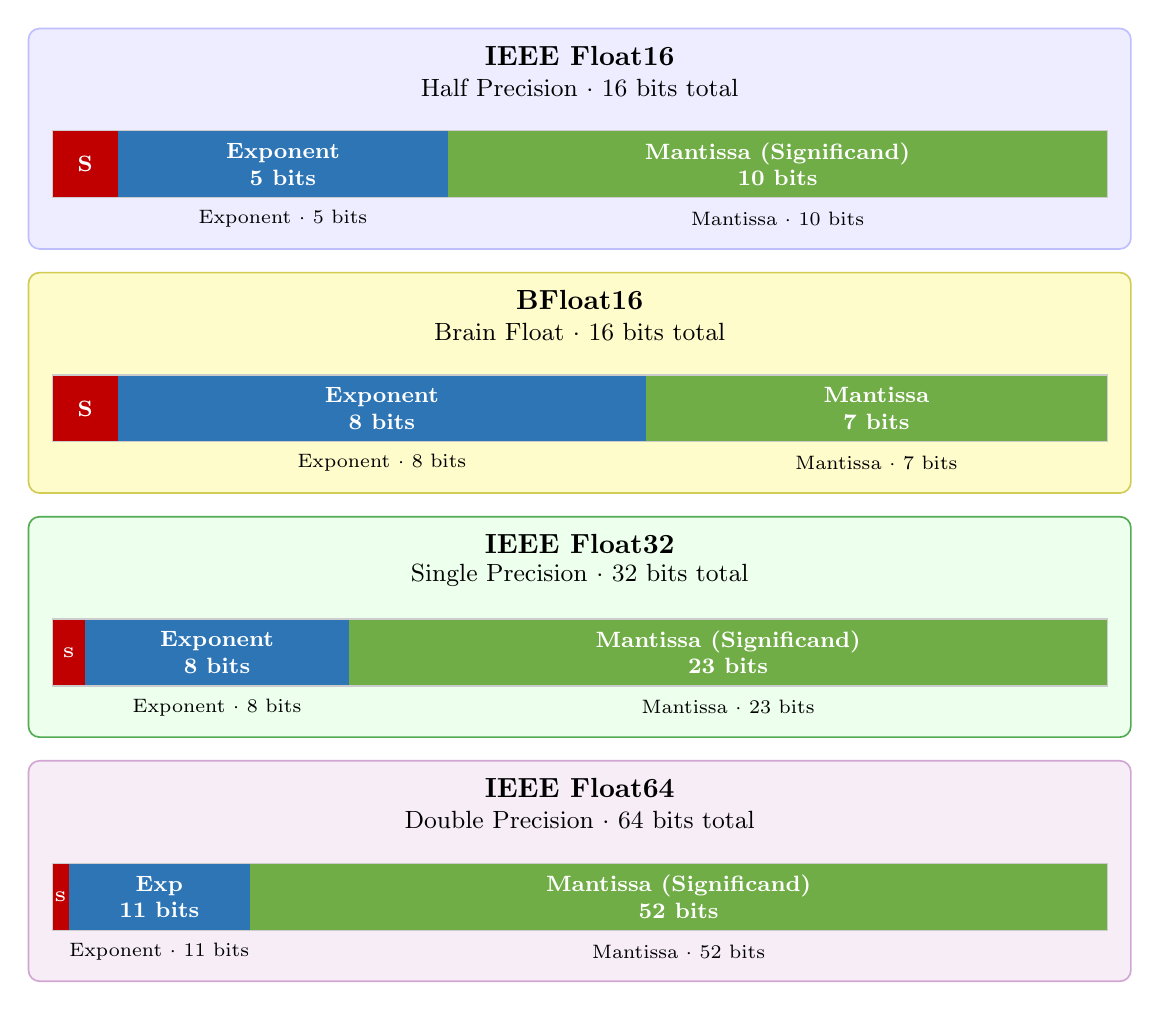
\begin{tikzpicture}[x=1cm, y=1cm]

  % ---- Color palette ----
  \definecolor{signcolor}{RGB}{192,0,0}     % red   -- sign bit
  \definecolor{expcolor} {RGB}{46,117,182}  % blue  -- exponent
  \definecolor{mancolor} {RGB}{112,173,71}  % green -- mantissa

  % ---- Panel backgrounds ----
  % Panels are 14 cm wide x 2.8 cm tall, separated by 0.3 cm gaps.
  % Y positions (bottom edge): Float16=9.30, BFloat16=6.20, Float32=3.10, Float64=0.00
  \draw[rounded corners=4pt, fill=blue!7,    draw=blue!25,        line width=0.6pt]
      (0.0,  9.30) rectangle (14.0, 12.10);  % Float16
  \draw[rounded corners=4pt, fill=yellow!20, draw=yellow!60!gray, line width=0.6pt]
      (0.0,  6.20) rectangle (14.0,  9.00);  % BFloat16
  \draw[rounded corners=4pt, fill=green!7,   draw=green!35!gray,  line width=0.6pt]
      (0.0,  3.10) rectangle (14.0,  5.90);  % Float32
  \draw[rounded corners=4pt, fill=violet!7,  draw=violet!35,      line width=0.6pt]
      (0.0,  0.00) rectangle (14.0,  2.80);  % Float64

  % ====================================================================
  % Bar geometry (shared across all panels):
  %   x range:    [0.30, 13.70]  => total bar width = 13.40 cm
  %   bar height: 0.85 cm
  %   bar bottom: panel_bottom + 0.65
  %   bar top:    panel_bottom + 1.50
  %
  % Segment x boundaries  (width = n_bits/total * 13.40):
  %   Float16  (16-bit): 0.300 | 1.138 | 5.325 | 13.700
  %   BFloat16 (16-bit): 0.300 | 1.138 | 7.838 | 13.700
  %   Float32  (32-bit): 0.300 | 0.719 | 4.069 | 13.700
  %   Float64  (64-bit): 0.300 | 0.509 | 2.813 | 13.700
  % ====================================================================

  % ------------------------------------------------------------------
  % IEEE Float16  (panel bottom y = 9.30)
  % ------------------------------------------------------------------
  \node[font=\normalsize\bfseries] at (7.0, 11.75) {IEEE Float16};
  \node[font=\small]               at (7.0, 11.35) {Half Precision $\cdot$ 16 bits total};

  % S:   1/16 * 13.40 = 0.838 cm   x: 0.300 -- 1.138,  center: 0.719
  \fill[signcolor] (0.300,  9.95) rectangle ( 1.138, 10.80);
  \node[text=white, font=\footnotesize\bfseries] at (0.719, 10.375) {S};

  % Exp: 5/16 * 13.40 = 4.188 cm   x: 1.138 -- 5.325,  center: 3.231
  \fill[expcolor]  (1.138,  9.95) rectangle ( 5.325, 10.80);
  \node[text=white, font=\footnotesize\bfseries, align=center] at (3.231, 10.375)
      {Exponent \\ 5 bits};

  % Man: 10/16 * 13.40 = 8.375 cm  x: 5.325 -- 13.700, center: 9.513
  \fill[mancolor]  (5.325,  9.95) rectangle (13.700, 10.80);
  \node[text=white, font=\footnotesize\bfseries, align=center] at (9.513, 10.375)
      {Mantissa (Significand) \\ 10 bits};

  \draw[black!20, line width=0.4pt] (0.300, 9.95) rectangle (13.700, 10.80);

  \node[font=\scriptsize] at (3.231, 9.68) {Exponent $\cdot$ 5 bits};
  \node[font=\scriptsize] at (9.513, 9.68) {Mantissa $\cdot$ 10 bits};

  % ------------------------------------------------------------------
  % BFloat16  (panel bottom y = 6.20)
  % ------------------------------------------------------------------
  \node[font=\normalsize\bfseries] at (7.0, 8.65) {BFloat16};
  \node[font=\small]               at (7.0, 8.25) {Brain Float $\cdot$ 16 bits total};

  % S:   1/16 * 13.40 = 0.838 cm   x: 0.300 -- 1.138,  center: 0.719
  \fill[signcolor] (0.300,  6.85) rectangle ( 1.138,  7.70);
  \node[text=white, font=\footnotesize\bfseries] at (0.719, 7.275) {S};

  % Exp: 8/16 * 13.40 = 6.700 cm   x: 1.138 -- 7.838,  center: 4.488
  \fill[expcolor]  (1.138,  6.85) rectangle ( 7.838,  7.70);
  \node[text=white, font=\footnotesize\bfseries, align=center] at (4.488, 7.275)
      {Exponent \\ 8 bits};

  % Man: 7/16 * 13.40 = 5.863 cm   x: 7.838 -- 13.700, center: 10.769
  \fill[mancolor]  (7.838,  6.85) rectangle (13.700,  7.70);
  \node[text=white, font=\footnotesize\bfseries, align=center] at (10.769, 7.275)
      {Mantissa \\ 7 bits};

  \draw[black!20, line width=0.4pt] (0.300, 6.85) rectangle (13.700, 7.70);

  \node[font=\scriptsize] at ( 4.488, 6.58) {Exponent $\cdot$ 8 bits};
  \node[font=\scriptsize] at (10.769, 6.58) {Mantissa $\cdot$ 7 bits};

  % ------------------------------------------------------------------
  % IEEE Float32  (panel bottom y = 3.10)
  % ------------------------------------------------------------------
  \node[font=\normalsize\bfseries] at (7.0, 5.55) {IEEE Float32};
  \node[font=\small]               at (7.0, 5.15) {Single Precision $\cdot$ 32 bits total};

  % S:   1/32 * 13.40 = 0.419 cm   x: 0.300 -- 0.719,  center: 0.510
  \fill[signcolor] (0.300,  3.75) rectangle ( 0.719,  4.60);
  \node[text=white, font=\tiny\bfseries] at (0.510, 4.175) {S};

  % Exp: 8/32 * 13.40 = 3.350 cm   x: 0.719 -- 4.069,  center: 2.394
  \fill[expcolor]  (0.719,  3.75) rectangle ( 4.069,  4.60);
  \node[text=white, font=\footnotesize\bfseries, align=center] at (2.394, 4.175)
      {Exponent \\ 8 bits};

  % Man: 23/32 * 13.40 = 9.631 cm  x: 4.069 -- 13.700, center: 8.885
  \fill[mancolor]  (4.069,  3.75) rectangle (13.700,  4.60);
  \node[text=white, font=\footnotesize\bfseries, align=center] at (8.885, 4.175)
      {Mantissa (Significand) \\ 23 bits};

  \draw[black!20, line width=0.4pt] (0.300, 3.75) rectangle (13.700, 4.60);

  \node[font=\scriptsize] at (2.394, 3.48) {Exponent $\cdot$ 8 bits};
  \node[font=\scriptsize] at (8.885, 3.48) {Mantissa $\cdot$ 23 bits};

  % ------------------------------------------------------------------
  % IEEE Float64  (panel bottom y = 0.00)
  % ------------------------------------------------------------------
  \node[font=\normalsize\bfseries] at (7.0, 2.45) {IEEE Float64};
  \node[font=\small]               at (7.0, 2.05) {Double Precision $\cdot$ 64 bits total};

  % S:    1/64 * 13.40 = 0.209 cm  x: 0.300 -- 0.509,  center: 0.405
  \fill[signcolor] (0.300,  0.65) rectangle ( 0.509,  1.50);
  \node[text=white, font=\tiny\bfseries] at (0.405, 1.075) {S};

  % Exp: 11/64 * 13.40 = 2.303 cm  x: 0.509 -- 2.813,  center: 1.661
  \fill[expcolor]  (0.509,  0.65) rectangle ( 2.813,  1.50);
  \node[text=white, font=\footnotesize\bfseries, align=center] at (1.661, 1.075)
      {Exp \\ 11 bits};

  % Man: 52/64 * 13.40 = 10.888 cm x: 2.813 -- 13.700, center: 8.257
  \fill[mancolor]  (2.813,  0.65) rectangle (13.700,  1.50);
  \node[text=white, font=\footnotesize\bfseries, align=center] at (8.257, 1.075)
      {Mantissa (Significand) \\ 52 bits};

  \draw[black!20, line width=0.4pt] (0.300, 0.65) rectangle (13.700, 1.50);

  \node[font=\scriptsize] at (1.661, 0.38) {Exponent $\cdot$ 11 bits};
  \node[font=\scriptsize] at (8.257, 0.38) {Mantissa $\cdot$ 52 bits};

\end{tikzpicture}
}
%     \caption{...}
%     \label{fig:float-formats}
%   \end{figure}
% --------------------------------------------------------------------
%
% Layout: 4 panels stacked vertically, each 14 cm x 2.8 cm.
% Bar widths are proportional to actual bit-field widths.
%   Float16:  S=1, Exp=5,  Man=10  (16 bits total)
%   BFloat16: S=1, Exp=8,  Man=7   (16 bits total)
%   Float32:  S=1, Exp=8,  Man=23  (32 bits total)
%   Float64:  S=1, Exp=11, Man=52  (64 bits total)

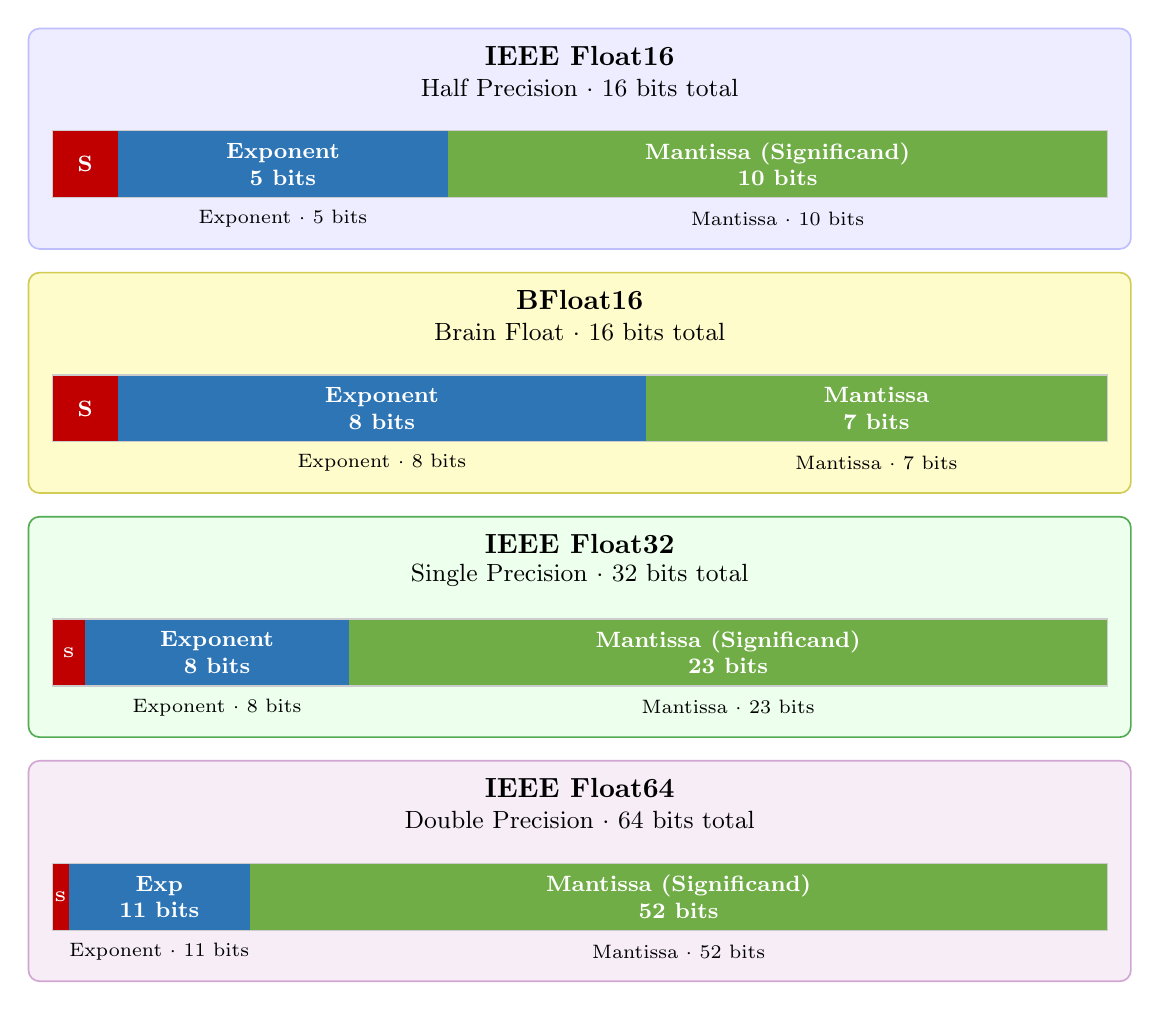
\begin{tikzpicture}[x=1cm, y=1cm]

  % ---- Color palette ----
  \definecolor{signcolor}{RGB}{192,0,0}     % red   -- sign bit
  \definecolor{expcolor} {RGB}{46,117,182}  % blue  -- exponent
  \definecolor{mancolor} {RGB}{112,173,71}  % green -- mantissa

  % ---- Panel backgrounds ----
  % Panels are 14 cm wide x 2.8 cm tall, separated by 0.3 cm gaps.
  % Y positions (bottom edge): Float16=9.30, BFloat16=6.20, Float32=3.10, Float64=0.00
  \draw[rounded corners=4pt, fill=blue!7,    draw=blue!25,        line width=0.6pt]
      (0.0,  9.30) rectangle (14.0, 12.10);  % Float16
  \draw[rounded corners=4pt, fill=yellow!20, draw=yellow!60!gray, line width=0.6pt]
      (0.0,  6.20) rectangle (14.0,  9.00);  % BFloat16
  \draw[rounded corners=4pt, fill=green!7,   draw=green!35!gray,  line width=0.6pt]
      (0.0,  3.10) rectangle (14.0,  5.90);  % Float32
  \draw[rounded corners=4pt, fill=violet!7,  draw=violet!35,      line width=0.6pt]
      (0.0,  0.00) rectangle (14.0,  2.80);  % Float64

  % ====================================================================
  % Bar geometry (shared across all panels):
  %   x range:    [0.30, 13.70]  => total bar width = 13.40 cm
  %   bar height: 0.85 cm
  %   bar bottom: panel_bottom + 0.65
  %   bar top:    panel_bottom + 1.50
  %
  % Segment x boundaries  (width = n_bits/total * 13.40):
  %   Float16  (16-bit): 0.300 | 1.138 | 5.325 | 13.700
  %   BFloat16 (16-bit): 0.300 | 1.138 | 7.838 | 13.700
  %   Float32  (32-bit): 0.300 | 0.719 | 4.069 | 13.700
  %   Float64  (64-bit): 0.300 | 0.509 | 2.813 | 13.700
  % ====================================================================

  % ------------------------------------------------------------------
  % IEEE Float16  (panel bottom y = 9.30)
  % ------------------------------------------------------------------
  \node[font=\normalsize\bfseries] at (7.0, 11.75) {IEEE Float16};
  \node[font=\small]               at (7.0, 11.35) {Half Precision $\cdot$ 16 bits total};

  % S:   1/16 * 13.40 = 0.838 cm   x: 0.300 -- 1.138,  center: 0.719
  \fill[signcolor] (0.300,  9.95) rectangle ( 1.138, 10.80);
  \node[text=white, font=\footnotesize\bfseries] at (0.719, 10.375) {S};

  % Exp: 5/16 * 13.40 = 4.188 cm   x: 1.138 -- 5.325,  center: 3.231
  \fill[expcolor]  (1.138,  9.95) rectangle ( 5.325, 10.80);
  \node[text=white, font=\footnotesize\bfseries, align=center] at (3.231, 10.375)
      {Exponent \\ 5 bits};

  % Man: 10/16 * 13.40 = 8.375 cm  x: 5.325 -- 13.700, center: 9.513
  \fill[mancolor]  (5.325,  9.95) rectangle (13.700, 10.80);
  \node[text=white, font=\footnotesize\bfseries, align=center] at (9.513, 10.375)
      {Mantissa (Significand) \\ 10 bits};

  \draw[black!20, line width=0.4pt] (0.300, 9.95) rectangle (13.700, 10.80);

  \node[font=\scriptsize] at (3.231, 9.68) {Exponent $\cdot$ 5 bits};
  \node[font=\scriptsize] at (9.513, 9.68) {Mantissa $\cdot$ 10 bits};

  % ------------------------------------------------------------------
  % BFloat16  (panel bottom y = 6.20)
  % ------------------------------------------------------------------
  \node[font=\normalsize\bfseries] at (7.0, 8.65) {BFloat16};
  \node[font=\small]               at (7.0, 8.25) {Brain Float $\cdot$ 16 bits total};

  % S:   1/16 * 13.40 = 0.838 cm   x: 0.300 -- 1.138,  center: 0.719
  \fill[signcolor] (0.300,  6.85) rectangle ( 1.138,  7.70);
  \node[text=white, font=\footnotesize\bfseries] at (0.719, 7.275) {S};

  % Exp: 8/16 * 13.40 = 6.700 cm   x: 1.138 -- 7.838,  center: 4.488
  \fill[expcolor]  (1.138,  6.85) rectangle ( 7.838,  7.70);
  \node[text=white, font=\footnotesize\bfseries, align=center] at (4.488, 7.275)
      {Exponent \\ 8 bits};

  % Man: 7/16 * 13.40 = 5.863 cm   x: 7.838 -- 13.700, center: 10.769
  \fill[mancolor]  (7.838,  6.85) rectangle (13.700,  7.70);
  \node[text=white, font=\footnotesize\bfseries, align=center] at (10.769, 7.275)
      {Mantissa \\ 7 bits};

  \draw[black!20, line width=0.4pt] (0.300, 6.85) rectangle (13.700, 7.70);

  \node[font=\scriptsize] at ( 4.488, 6.58) {Exponent $\cdot$ 8 bits};
  \node[font=\scriptsize] at (10.769, 6.58) {Mantissa $\cdot$ 7 bits};

  % ------------------------------------------------------------------
  % IEEE Float32  (panel bottom y = 3.10)
  % ------------------------------------------------------------------
  \node[font=\normalsize\bfseries] at (7.0, 5.55) {IEEE Float32};
  \node[font=\small]               at (7.0, 5.15) {Single Precision $\cdot$ 32 bits total};

  % S:   1/32 * 13.40 = 0.419 cm   x: 0.300 -- 0.719,  center: 0.510
  \fill[signcolor] (0.300,  3.75) rectangle ( 0.719,  4.60);
  \node[text=white, font=\tiny\bfseries] at (0.510, 4.175) {S};

  % Exp: 8/32 * 13.40 = 3.350 cm   x: 0.719 -- 4.069,  center: 2.394
  \fill[expcolor]  (0.719,  3.75) rectangle ( 4.069,  4.60);
  \node[text=white, font=\footnotesize\bfseries, align=center] at (2.394, 4.175)
      {Exponent \\ 8 bits};

  % Man: 23/32 * 13.40 = 9.631 cm  x: 4.069 -- 13.700, center: 8.885
  \fill[mancolor]  (4.069,  3.75) rectangle (13.700,  4.60);
  \node[text=white, font=\footnotesize\bfseries, align=center] at (8.885, 4.175)
      {Mantissa (Significand) \\ 23 bits};

  \draw[black!20, line width=0.4pt] (0.300, 3.75) rectangle (13.700, 4.60);

  \node[font=\scriptsize] at (2.394, 3.48) {Exponent $\cdot$ 8 bits};
  \node[font=\scriptsize] at (8.885, 3.48) {Mantissa $\cdot$ 23 bits};

  % ------------------------------------------------------------------
  % IEEE Float64  (panel bottom y = 0.00)
  % ------------------------------------------------------------------
  \node[font=\normalsize\bfseries] at (7.0, 2.45) {IEEE Float64};
  \node[font=\small]               at (7.0, 2.05) {Double Precision $\cdot$ 64 bits total};

  % S:    1/64 * 13.40 = 0.209 cm  x: 0.300 -- 0.509,  center: 0.405
  \fill[signcolor] (0.300,  0.65) rectangle ( 0.509,  1.50);
  \node[text=white, font=\tiny\bfseries] at (0.405, 1.075) {S};

  % Exp: 11/64 * 13.40 = 2.303 cm  x: 0.509 -- 2.813,  center: 1.661
  \fill[expcolor]  (0.509,  0.65) rectangle ( 2.813,  1.50);
  \node[text=white, font=\footnotesize\bfseries, align=center] at (1.661, 1.075)
      {Exp \\ 11 bits};

  % Man: 52/64 * 13.40 = 10.888 cm x: 2.813 -- 13.700, center: 8.257
  \fill[mancolor]  (2.813,  0.65) rectangle (13.700,  1.50);
  \node[text=white, font=\footnotesize\bfseries, align=center] at (8.257, 1.075)
      {Mantissa (Significand) \\ 52 bits};

  \draw[black!20, line width=0.4pt] (0.300, 0.65) rectangle (13.700, 1.50);

  \node[font=\scriptsize] at (1.661, 0.38) {Exponent $\cdot$ 11 bits};
  \node[font=\scriptsize] at (8.257, 0.38) {Mantissa $\cdot$ 52 bits};

\end{tikzpicture}
}
%     \caption{...}
%     \label{fig:float-formats}
%   \end{figure}
% --------------------------------------------------------------------
%
% Layout: 4 panels stacked vertically, each 14 cm x 2.8 cm.
% Bar widths are proportional to actual bit-field widths.
%   Float16:  S=1, Exp=5,  Man=10  (16 bits total)
%   BFloat16: S=1, Exp=8,  Man=7   (16 bits total)
%   Float32:  S=1, Exp=8,  Man=23  (32 bits total)
%   Float64:  S=1, Exp=11, Man=52  (64 bits total)

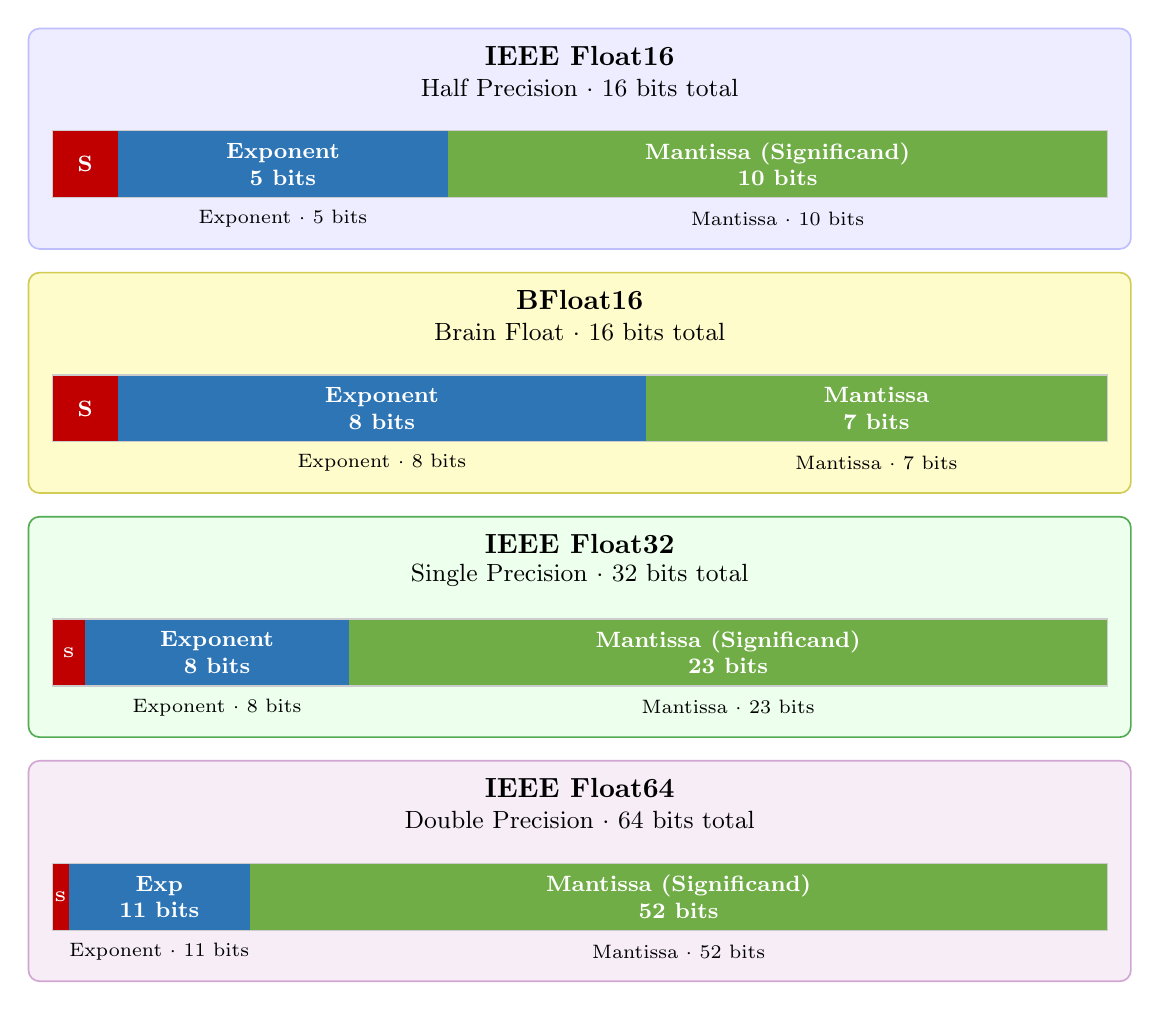
\begin{tikzpicture}[x=1cm, y=1cm]

  % ---- Color palette ----
  \definecolor{signcolor}{RGB}{192,0,0}     % red   -- sign bit
  \definecolor{expcolor} {RGB}{46,117,182}  % blue  -- exponent
  \definecolor{mancolor} {RGB}{112,173,71}  % green -- mantissa

  % ---- Panel backgrounds ----
  % Panels are 14 cm wide x 2.8 cm tall, separated by 0.3 cm gaps.
  % Y positions (bottom edge): Float16=9.30, BFloat16=6.20, Float32=3.10, Float64=0.00
  \draw[rounded corners=4pt, fill=blue!7,    draw=blue!25,        line width=0.6pt]
      (0.0,  9.30) rectangle (14.0, 12.10);  % Float16
  \draw[rounded corners=4pt, fill=yellow!20, draw=yellow!60!gray, line width=0.6pt]
      (0.0,  6.20) rectangle (14.0,  9.00);  % BFloat16
  \draw[rounded corners=4pt, fill=green!7,   draw=green!35!gray,  line width=0.6pt]
      (0.0,  3.10) rectangle (14.0,  5.90);  % Float32
  \draw[rounded corners=4pt, fill=violet!7,  draw=violet!35,      line width=0.6pt]
      (0.0,  0.00) rectangle (14.0,  2.80);  % Float64

  % ====================================================================
  % Bar geometry (shared across all panels):
  %   x range:    [0.30, 13.70]  => total bar width = 13.40 cm
  %   bar height: 0.85 cm
  %   bar bottom: panel_bottom + 0.65
  %   bar top:    panel_bottom + 1.50
  %
  % Segment x boundaries  (width = n_bits/total * 13.40):
  %   Float16  (16-bit): 0.300 | 1.138 | 5.325 | 13.700
  %   BFloat16 (16-bit): 0.300 | 1.138 | 7.838 | 13.700
  %   Float32  (32-bit): 0.300 | 0.719 | 4.069 | 13.700
  %   Float64  (64-bit): 0.300 | 0.509 | 2.813 | 13.700
  % ====================================================================

  % ------------------------------------------------------------------
  % IEEE Float16  (panel bottom y = 9.30)
  % ------------------------------------------------------------------
  \node[font=\normalsize\bfseries] at (7.0, 11.75) {IEEE Float16};
  \node[font=\small]               at (7.0, 11.35) {Half Precision $\cdot$ 16 bits total};

  % S:   1/16 * 13.40 = 0.838 cm   x: 0.300 -- 1.138,  center: 0.719
  \fill[signcolor] (0.300,  9.95) rectangle ( 1.138, 10.80);
  \node[text=white, font=\footnotesize\bfseries] at (0.719, 10.375) {S};

  % Exp: 5/16 * 13.40 = 4.188 cm   x: 1.138 -- 5.325,  center: 3.231
  \fill[expcolor]  (1.138,  9.95) rectangle ( 5.325, 10.80);
  \node[text=white, font=\footnotesize\bfseries, align=center] at (3.231, 10.375)
      {Exponent \\ 5 bits};

  % Man: 10/16 * 13.40 = 8.375 cm  x: 5.325 -- 13.700, center: 9.513
  \fill[mancolor]  (5.325,  9.95) rectangle (13.700, 10.80);
  \node[text=white, font=\footnotesize\bfseries, align=center] at (9.513, 10.375)
      {Mantissa (Significand) \\ 10 bits};

  \draw[black!20, line width=0.4pt] (0.300, 9.95) rectangle (13.700, 10.80);

  \node[font=\scriptsize] at (3.231, 9.68) {Exponent $\cdot$ 5 bits};
  \node[font=\scriptsize] at (9.513, 9.68) {Mantissa $\cdot$ 10 bits};

  % ------------------------------------------------------------------
  % BFloat16  (panel bottom y = 6.20)
  % ------------------------------------------------------------------
  \node[font=\normalsize\bfseries] at (7.0, 8.65) {BFloat16};
  \node[font=\small]               at (7.0, 8.25) {Brain Float $\cdot$ 16 bits total};

  % S:   1/16 * 13.40 = 0.838 cm   x: 0.300 -- 1.138,  center: 0.719
  \fill[signcolor] (0.300,  6.85) rectangle ( 1.138,  7.70);
  \node[text=white, font=\footnotesize\bfseries] at (0.719, 7.275) {S};

  % Exp: 8/16 * 13.40 = 6.700 cm   x: 1.138 -- 7.838,  center: 4.488
  \fill[expcolor]  (1.138,  6.85) rectangle ( 7.838,  7.70);
  \node[text=white, font=\footnotesize\bfseries, align=center] at (4.488, 7.275)
      {Exponent \\ 8 bits};

  % Man: 7/16 * 13.40 = 5.863 cm   x: 7.838 -- 13.700, center: 10.769
  \fill[mancolor]  (7.838,  6.85) rectangle (13.700,  7.70);
  \node[text=white, font=\footnotesize\bfseries, align=center] at (10.769, 7.275)
      {Mantissa \\ 7 bits};

  \draw[black!20, line width=0.4pt] (0.300, 6.85) rectangle (13.700, 7.70);

  \node[font=\scriptsize] at ( 4.488, 6.58) {Exponent $\cdot$ 8 bits};
  \node[font=\scriptsize] at (10.769, 6.58) {Mantissa $\cdot$ 7 bits};

  % ------------------------------------------------------------------
  % IEEE Float32  (panel bottom y = 3.10)
  % ------------------------------------------------------------------
  \node[font=\normalsize\bfseries] at (7.0, 5.55) {IEEE Float32};
  \node[font=\small]               at (7.0, 5.15) {Single Precision $\cdot$ 32 bits total};

  % S:   1/32 * 13.40 = 0.419 cm   x: 0.300 -- 0.719,  center: 0.510
  \fill[signcolor] (0.300,  3.75) rectangle ( 0.719,  4.60);
  \node[text=white, font=\tiny\bfseries] at (0.510, 4.175) {S};

  % Exp: 8/32 * 13.40 = 3.350 cm   x: 0.719 -- 4.069,  center: 2.394
  \fill[expcolor]  (0.719,  3.75) rectangle ( 4.069,  4.60);
  \node[text=white, font=\footnotesize\bfseries, align=center] at (2.394, 4.175)
      {Exponent \\ 8 bits};

  % Man: 23/32 * 13.40 = 9.631 cm  x: 4.069 -- 13.700, center: 8.885
  \fill[mancolor]  (4.069,  3.75) rectangle (13.700,  4.60);
  \node[text=white, font=\footnotesize\bfseries, align=center] at (8.885, 4.175)
      {Mantissa (Significand) \\ 23 bits};

  \draw[black!20, line width=0.4pt] (0.300, 3.75) rectangle (13.700, 4.60);

  \node[font=\scriptsize] at (2.394, 3.48) {Exponent $\cdot$ 8 bits};
  \node[font=\scriptsize] at (8.885, 3.48) {Mantissa $\cdot$ 23 bits};

  % ------------------------------------------------------------------
  % IEEE Float64  (panel bottom y = 0.00)
  % ------------------------------------------------------------------
  \node[font=\normalsize\bfseries] at (7.0, 2.45) {IEEE Float64};
  \node[font=\small]               at (7.0, 2.05) {Double Precision $\cdot$ 64 bits total};

  % S:    1/64 * 13.40 = 0.209 cm  x: 0.300 -- 0.509,  center: 0.405
  \fill[signcolor] (0.300,  0.65) rectangle ( 0.509,  1.50);
  \node[text=white, font=\tiny\bfseries] at (0.405, 1.075) {S};

  % Exp: 11/64 * 13.40 = 2.303 cm  x: 0.509 -- 2.813,  center: 1.661
  \fill[expcolor]  (0.509,  0.65) rectangle ( 2.813,  1.50);
  \node[text=white, font=\footnotesize\bfseries, align=center] at (1.661, 1.075)
      {Exp \\ 11 bits};

  % Man: 52/64 * 13.40 = 10.888 cm x: 2.813 -- 13.700, center: 8.257
  \fill[mancolor]  (2.813,  0.65) rectangle (13.700,  1.50);
  \node[text=white, font=\footnotesize\bfseries, align=center] at (8.257, 1.075)
      {Mantissa (Significand) \\ 52 bits};

  \draw[black!20, line width=0.4pt] (0.300, 0.65) rectangle (13.700, 1.50);

  \node[font=\scriptsize] at (1.661, 0.38) {Exponent $\cdot$ 11 bits};
  \node[font=\scriptsize] at (8.257, 0.38) {Mantissa $\cdot$ 52 bits};

\end{tikzpicture}
}
%
%   Fit to an arbitrary fraction of the column width:
%     \resizebox{0.9\columnwidth}{!}{% Floating-point format comparison — single-column stack layout
%
% Required in preamble:
%   \usepackage{tikz}
%
% ---- Scaling -------------------------------------------------------
% The tikzpicture is drawn at its natural size: 14 cm wide x 12.1 cm tall.
% Use \resizebox (from the graphicx package, always loaded in IEEE style)
% to scale it to whatever width you need. The height adjusts automatically.
%
%   Fit to a single text column (~8.8 cm in IEEE two-column):
%     \resizebox{\columnwidth}{!}{% Floating-point format comparison — single-column stack layout
%
% Required in preamble:
%   \usepackage{tikz}
%
% ---- Scaling -------------------------------------------------------
% The tikzpicture is drawn at its natural size: 14 cm wide x 12.1 cm tall.
% Use \resizebox (from the graphicx package, always loaded in IEEE style)
% to scale it to whatever width you need. The height adjusts automatically.
%
%   Fit to a single text column (~8.8 cm in IEEE two-column):
%     \resizebox{\columnwidth}{!}{% Floating-point format comparison — single-column stack layout
%
% Required in preamble:
%   \usepackage{tikz}
%
% ---- Scaling -------------------------------------------------------
% The tikzpicture is drawn at its natural size: 14 cm wide x 12.1 cm tall.
% Use \resizebox (from the graphicx package, always loaded in IEEE style)
% to scale it to whatever width you need. The height adjusts automatically.
%
%   Fit to a single text column (~8.8 cm in IEEE two-column):
%     \resizebox{\columnwidth}{!}{\input{float_formats_tikz.tex}}
%
%   Fit to the full page width (~17.8 cm in IEEE two-column):
%     \resizebox{\textwidth}{!}{\input{float_formats_tikz.tex}}
%
%   Fit to an arbitrary fraction of the column width:
%     \resizebox{0.9\columnwidth}{!}{\input{float_formats_tikz.tex}}
%
% \resizebox scales everything uniformly — coordinates, line widths,
% and fonts — so the result looks identical regardless of the chosen width.
%
% Recommended figure wrapper (single column):
%   \begin{figure}[t]
%     \centering
%     \resizebox{\columnwidth}{!}{\input{float_formats_tikz.tex}}
%     \caption{...}
%     \label{fig:float-formats}
%   \end{figure}
% --------------------------------------------------------------------
%
% Layout: 4 panels stacked vertically, each 14 cm x 2.8 cm.
% Bar widths are proportional to actual bit-field widths.
%   Float16:  S=1, Exp=5,  Man=10  (16 bits total)
%   BFloat16: S=1, Exp=8,  Man=7   (16 bits total)
%   Float32:  S=1, Exp=8,  Man=23  (32 bits total)
%   Float64:  S=1, Exp=11, Man=52  (64 bits total)

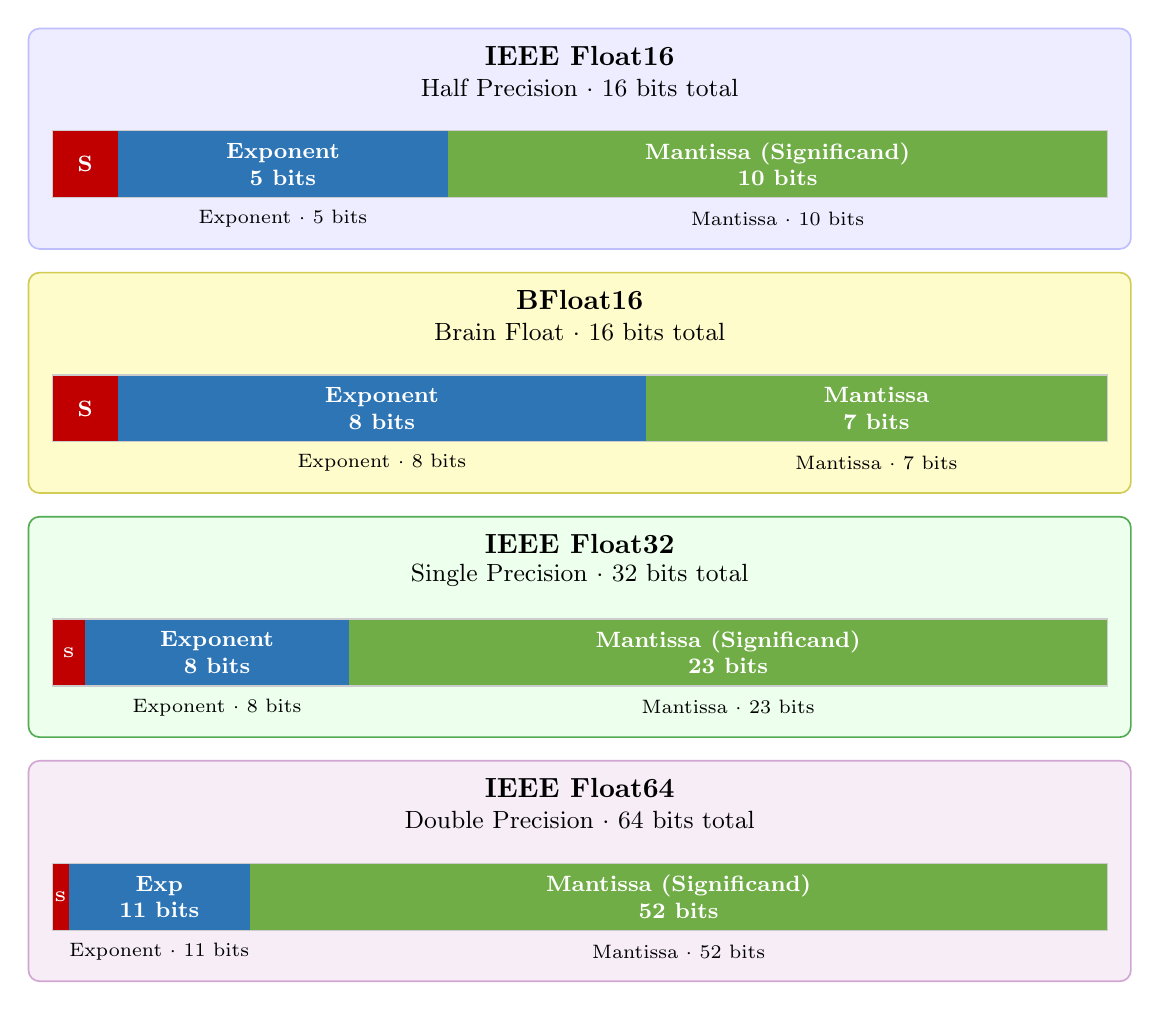
\begin{tikzpicture}[x=1cm, y=1cm]

  % ---- Color palette ----
  \definecolor{signcolor}{RGB}{192,0,0}     % red   -- sign bit
  \definecolor{expcolor} {RGB}{46,117,182}  % blue  -- exponent
  \definecolor{mancolor} {RGB}{112,173,71}  % green -- mantissa

  % ---- Panel backgrounds ----
  % Panels are 14 cm wide x 2.8 cm tall, separated by 0.3 cm gaps.
  % Y positions (bottom edge): Float16=9.30, BFloat16=6.20, Float32=3.10, Float64=0.00
  \draw[rounded corners=4pt, fill=blue!7,    draw=blue!25,        line width=0.6pt]
      (0.0,  9.30) rectangle (14.0, 12.10);  % Float16
  \draw[rounded corners=4pt, fill=yellow!20, draw=yellow!60!gray, line width=0.6pt]
      (0.0,  6.20) rectangle (14.0,  9.00);  % BFloat16
  \draw[rounded corners=4pt, fill=green!7,   draw=green!35!gray,  line width=0.6pt]
      (0.0,  3.10) rectangle (14.0,  5.90);  % Float32
  \draw[rounded corners=4pt, fill=violet!7,  draw=violet!35,      line width=0.6pt]
      (0.0,  0.00) rectangle (14.0,  2.80);  % Float64

  % ====================================================================
  % Bar geometry (shared across all panels):
  %   x range:    [0.30, 13.70]  => total bar width = 13.40 cm
  %   bar height: 0.85 cm
  %   bar bottom: panel_bottom + 0.65
  %   bar top:    panel_bottom + 1.50
  %
  % Segment x boundaries  (width = n_bits/total * 13.40):
  %   Float16  (16-bit): 0.300 | 1.138 | 5.325 | 13.700
  %   BFloat16 (16-bit): 0.300 | 1.138 | 7.838 | 13.700
  %   Float32  (32-bit): 0.300 | 0.719 | 4.069 | 13.700
  %   Float64  (64-bit): 0.300 | 0.509 | 2.813 | 13.700
  % ====================================================================

  % ------------------------------------------------------------------
  % IEEE Float16  (panel bottom y = 9.30)
  % ------------------------------------------------------------------
  \node[font=\normalsize\bfseries] at (7.0, 11.75) {IEEE Float16};
  \node[font=\small]               at (7.0, 11.35) {Half Precision $\cdot$ 16 bits total};

  % S:   1/16 * 13.40 = 0.838 cm   x: 0.300 -- 1.138,  center: 0.719
  \fill[signcolor] (0.300,  9.95) rectangle ( 1.138, 10.80);
  \node[text=white, font=\footnotesize\bfseries] at (0.719, 10.375) {S};

  % Exp: 5/16 * 13.40 = 4.188 cm   x: 1.138 -- 5.325,  center: 3.231
  \fill[expcolor]  (1.138,  9.95) rectangle ( 5.325, 10.80);
  \node[text=white, font=\footnotesize\bfseries, align=center] at (3.231, 10.375)
      {Exponent \\ 5 bits};

  % Man: 10/16 * 13.40 = 8.375 cm  x: 5.325 -- 13.700, center: 9.513
  \fill[mancolor]  (5.325,  9.95) rectangle (13.700, 10.80);
  \node[text=white, font=\footnotesize\bfseries, align=center] at (9.513, 10.375)
      {Mantissa (Significand) \\ 10 bits};

  \draw[black!20, line width=0.4pt] (0.300, 9.95) rectangle (13.700, 10.80);

  \node[font=\scriptsize] at (3.231, 9.68) {Exponent $\cdot$ 5 bits};
  \node[font=\scriptsize] at (9.513, 9.68) {Mantissa $\cdot$ 10 bits};

  % ------------------------------------------------------------------
  % BFloat16  (panel bottom y = 6.20)
  % ------------------------------------------------------------------
  \node[font=\normalsize\bfseries] at (7.0, 8.65) {BFloat16};
  \node[font=\small]               at (7.0, 8.25) {Brain Float $\cdot$ 16 bits total};

  % S:   1/16 * 13.40 = 0.838 cm   x: 0.300 -- 1.138,  center: 0.719
  \fill[signcolor] (0.300,  6.85) rectangle ( 1.138,  7.70);
  \node[text=white, font=\footnotesize\bfseries] at (0.719, 7.275) {S};

  % Exp: 8/16 * 13.40 = 6.700 cm   x: 1.138 -- 7.838,  center: 4.488
  \fill[expcolor]  (1.138,  6.85) rectangle ( 7.838,  7.70);
  \node[text=white, font=\footnotesize\bfseries, align=center] at (4.488, 7.275)
      {Exponent \\ 8 bits};

  % Man: 7/16 * 13.40 = 5.863 cm   x: 7.838 -- 13.700, center: 10.769
  \fill[mancolor]  (7.838,  6.85) rectangle (13.700,  7.70);
  \node[text=white, font=\footnotesize\bfseries, align=center] at (10.769, 7.275)
      {Mantissa \\ 7 bits};

  \draw[black!20, line width=0.4pt] (0.300, 6.85) rectangle (13.700, 7.70);

  \node[font=\scriptsize] at ( 4.488, 6.58) {Exponent $\cdot$ 8 bits};
  \node[font=\scriptsize] at (10.769, 6.58) {Mantissa $\cdot$ 7 bits};

  % ------------------------------------------------------------------
  % IEEE Float32  (panel bottom y = 3.10)
  % ------------------------------------------------------------------
  \node[font=\normalsize\bfseries] at (7.0, 5.55) {IEEE Float32};
  \node[font=\small]               at (7.0, 5.15) {Single Precision $\cdot$ 32 bits total};

  % S:   1/32 * 13.40 = 0.419 cm   x: 0.300 -- 0.719,  center: 0.510
  \fill[signcolor] (0.300,  3.75) rectangle ( 0.719,  4.60);
  \node[text=white, font=\tiny\bfseries] at (0.510, 4.175) {S};

  % Exp: 8/32 * 13.40 = 3.350 cm   x: 0.719 -- 4.069,  center: 2.394
  \fill[expcolor]  (0.719,  3.75) rectangle ( 4.069,  4.60);
  \node[text=white, font=\footnotesize\bfseries, align=center] at (2.394, 4.175)
      {Exponent \\ 8 bits};

  % Man: 23/32 * 13.40 = 9.631 cm  x: 4.069 -- 13.700, center: 8.885
  \fill[mancolor]  (4.069,  3.75) rectangle (13.700,  4.60);
  \node[text=white, font=\footnotesize\bfseries, align=center] at (8.885, 4.175)
      {Mantissa (Significand) \\ 23 bits};

  \draw[black!20, line width=0.4pt] (0.300, 3.75) rectangle (13.700, 4.60);

  \node[font=\scriptsize] at (2.394, 3.48) {Exponent $\cdot$ 8 bits};
  \node[font=\scriptsize] at (8.885, 3.48) {Mantissa $\cdot$ 23 bits};

  % ------------------------------------------------------------------
  % IEEE Float64  (panel bottom y = 0.00)
  % ------------------------------------------------------------------
  \node[font=\normalsize\bfseries] at (7.0, 2.45) {IEEE Float64};
  \node[font=\small]               at (7.0, 2.05) {Double Precision $\cdot$ 64 bits total};

  % S:    1/64 * 13.40 = 0.209 cm  x: 0.300 -- 0.509,  center: 0.405
  \fill[signcolor] (0.300,  0.65) rectangle ( 0.509,  1.50);
  \node[text=white, font=\tiny\bfseries] at (0.405, 1.075) {S};

  % Exp: 11/64 * 13.40 = 2.303 cm  x: 0.509 -- 2.813,  center: 1.661
  \fill[expcolor]  (0.509,  0.65) rectangle ( 2.813,  1.50);
  \node[text=white, font=\footnotesize\bfseries, align=center] at (1.661, 1.075)
      {Exp \\ 11 bits};

  % Man: 52/64 * 13.40 = 10.888 cm x: 2.813 -- 13.700, center: 8.257
  \fill[mancolor]  (2.813,  0.65) rectangle (13.700,  1.50);
  \node[text=white, font=\footnotesize\bfseries, align=center] at (8.257, 1.075)
      {Mantissa (Significand) \\ 52 bits};

  \draw[black!20, line width=0.4pt] (0.300, 0.65) rectangle (13.700, 1.50);

  \node[font=\scriptsize] at (1.661, 0.38) {Exponent $\cdot$ 11 bits};
  \node[font=\scriptsize] at (8.257, 0.38) {Mantissa $\cdot$ 52 bits};

\end{tikzpicture}
}
%
%   Fit to the full page width (~17.8 cm in IEEE two-column):
%     \resizebox{\textwidth}{!}{% Floating-point format comparison — single-column stack layout
%
% Required in preamble:
%   \usepackage{tikz}
%
% ---- Scaling -------------------------------------------------------
% The tikzpicture is drawn at its natural size: 14 cm wide x 12.1 cm tall.
% Use \resizebox (from the graphicx package, always loaded in IEEE style)
% to scale it to whatever width you need. The height adjusts automatically.
%
%   Fit to a single text column (~8.8 cm in IEEE two-column):
%     \resizebox{\columnwidth}{!}{\input{float_formats_tikz.tex}}
%
%   Fit to the full page width (~17.8 cm in IEEE two-column):
%     \resizebox{\textwidth}{!}{\input{float_formats_tikz.tex}}
%
%   Fit to an arbitrary fraction of the column width:
%     \resizebox{0.9\columnwidth}{!}{\input{float_formats_tikz.tex}}
%
% \resizebox scales everything uniformly — coordinates, line widths,
% and fonts — so the result looks identical regardless of the chosen width.
%
% Recommended figure wrapper (single column):
%   \begin{figure}[t]
%     \centering
%     \resizebox{\columnwidth}{!}{\input{float_formats_tikz.tex}}
%     \caption{...}
%     \label{fig:float-formats}
%   \end{figure}
% --------------------------------------------------------------------
%
% Layout: 4 panels stacked vertically, each 14 cm x 2.8 cm.
% Bar widths are proportional to actual bit-field widths.
%   Float16:  S=1, Exp=5,  Man=10  (16 bits total)
%   BFloat16: S=1, Exp=8,  Man=7   (16 bits total)
%   Float32:  S=1, Exp=8,  Man=23  (32 bits total)
%   Float64:  S=1, Exp=11, Man=52  (64 bits total)

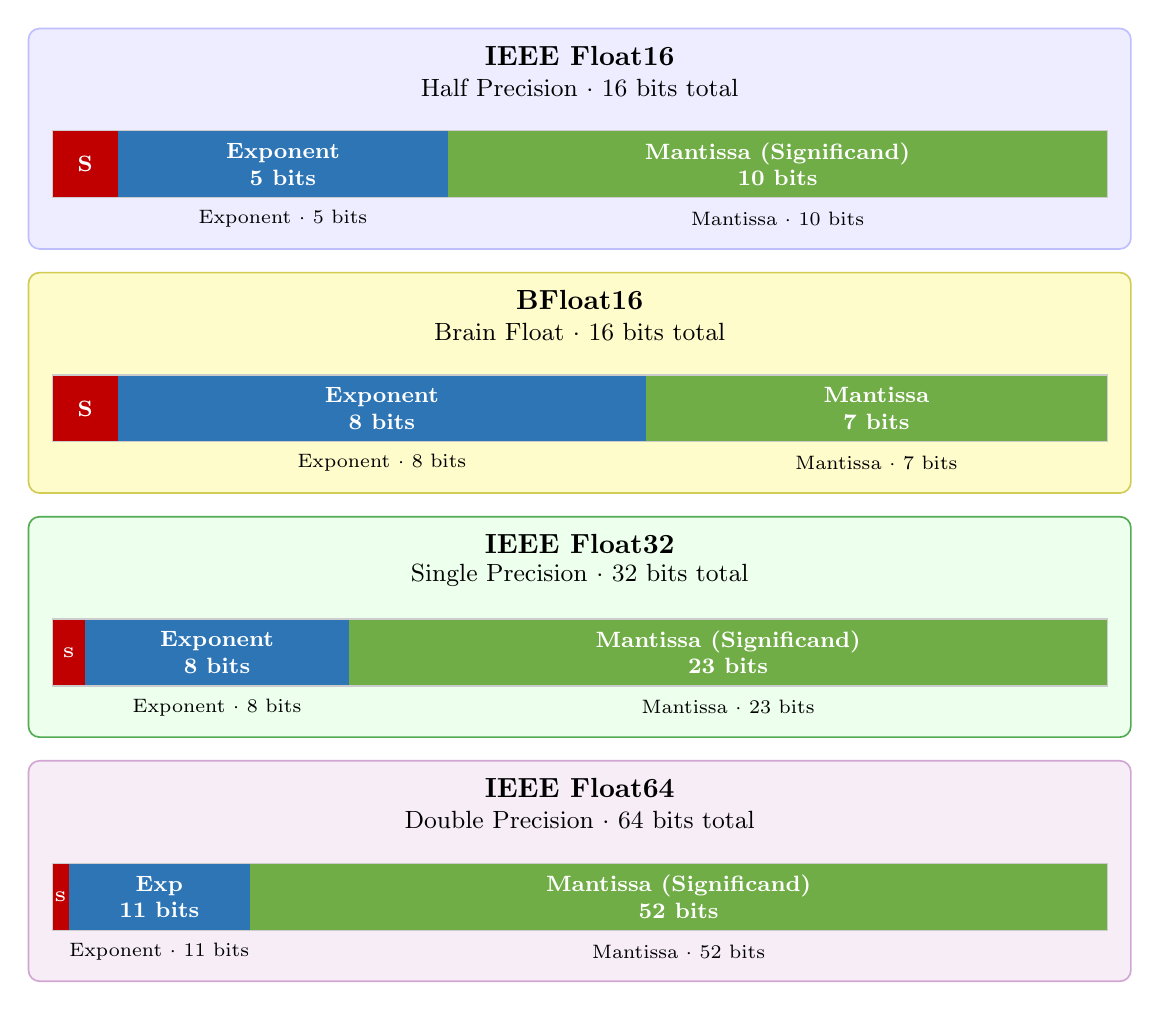
\begin{tikzpicture}[x=1cm, y=1cm]

  % ---- Color palette ----
  \definecolor{signcolor}{RGB}{192,0,0}     % red   -- sign bit
  \definecolor{expcolor} {RGB}{46,117,182}  % blue  -- exponent
  \definecolor{mancolor} {RGB}{112,173,71}  % green -- mantissa

  % ---- Panel backgrounds ----
  % Panels are 14 cm wide x 2.8 cm tall, separated by 0.3 cm gaps.
  % Y positions (bottom edge): Float16=9.30, BFloat16=6.20, Float32=3.10, Float64=0.00
  \draw[rounded corners=4pt, fill=blue!7,    draw=blue!25,        line width=0.6pt]
      (0.0,  9.30) rectangle (14.0, 12.10);  % Float16
  \draw[rounded corners=4pt, fill=yellow!20, draw=yellow!60!gray, line width=0.6pt]
      (0.0,  6.20) rectangle (14.0,  9.00);  % BFloat16
  \draw[rounded corners=4pt, fill=green!7,   draw=green!35!gray,  line width=0.6pt]
      (0.0,  3.10) rectangle (14.0,  5.90);  % Float32
  \draw[rounded corners=4pt, fill=violet!7,  draw=violet!35,      line width=0.6pt]
      (0.0,  0.00) rectangle (14.0,  2.80);  % Float64

  % ====================================================================
  % Bar geometry (shared across all panels):
  %   x range:    [0.30, 13.70]  => total bar width = 13.40 cm
  %   bar height: 0.85 cm
  %   bar bottom: panel_bottom + 0.65
  %   bar top:    panel_bottom + 1.50
  %
  % Segment x boundaries  (width = n_bits/total * 13.40):
  %   Float16  (16-bit): 0.300 | 1.138 | 5.325 | 13.700
  %   BFloat16 (16-bit): 0.300 | 1.138 | 7.838 | 13.700
  %   Float32  (32-bit): 0.300 | 0.719 | 4.069 | 13.700
  %   Float64  (64-bit): 0.300 | 0.509 | 2.813 | 13.700
  % ====================================================================

  % ------------------------------------------------------------------
  % IEEE Float16  (panel bottom y = 9.30)
  % ------------------------------------------------------------------
  \node[font=\normalsize\bfseries] at (7.0, 11.75) {IEEE Float16};
  \node[font=\small]               at (7.0, 11.35) {Half Precision $\cdot$ 16 bits total};

  % S:   1/16 * 13.40 = 0.838 cm   x: 0.300 -- 1.138,  center: 0.719
  \fill[signcolor] (0.300,  9.95) rectangle ( 1.138, 10.80);
  \node[text=white, font=\footnotesize\bfseries] at (0.719, 10.375) {S};

  % Exp: 5/16 * 13.40 = 4.188 cm   x: 1.138 -- 5.325,  center: 3.231
  \fill[expcolor]  (1.138,  9.95) rectangle ( 5.325, 10.80);
  \node[text=white, font=\footnotesize\bfseries, align=center] at (3.231, 10.375)
      {Exponent \\ 5 bits};

  % Man: 10/16 * 13.40 = 8.375 cm  x: 5.325 -- 13.700, center: 9.513
  \fill[mancolor]  (5.325,  9.95) rectangle (13.700, 10.80);
  \node[text=white, font=\footnotesize\bfseries, align=center] at (9.513, 10.375)
      {Mantissa (Significand) \\ 10 bits};

  \draw[black!20, line width=0.4pt] (0.300, 9.95) rectangle (13.700, 10.80);

  \node[font=\scriptsize] at (3.231, 9.68) {Exponent $\cdot$ 5 bits};
  \node[font=\scriptsize] at (9.513, 9.68) {Mantissa $\cdot$ 10 bits};

  % ------------------------------------------------------------------
  % BFloat16  (panel bottom y = 6.20)
  % ------------------------------------------------------------------
  \node[font=\normalsize\bfseries] at (7.0, 8.65) {BFloat16};
  \node[font=\small]               at (7.0, 8.25) {Brain Float $\cdot$ 16 bits total};

  % S:   1/16 * 13.40 = 0.838 cm   x: 0.300 -- 1.138,  center: 0.719
  \fill[signcolor] (0.300,  6.85) rectangle ( 1.138,  7.70);
  \node[text=white, font=\footnotesize\bfseries] at (0.719, 7.275) {S};

  % Exp: 8/16 * 13.40 = 6.700 cm   x: 1.138 -- 7.838,  center: 4.488
  \fill[expcolor]  (1.138,  6.85) rectangle ( 7.838,  7.70);
  \node[text=white, font=\footnotesize\bfseries, align=center] at (4.488, 7.275)
      {Exponent \\ 8 bits};

  % Man: 7/16 * 13.40 = 5.863 cm   x: 7.838 -- 13.700, center: 10.769
  \fill[mancolor]  (7.838,  6.85) rectangle (13.700,  7.70);
  \node[text=white, font=\footnotesize\bfseries, align=center] at (10.769, 7.275)
      {Mantissa \\ 7 bits};

  \draw[black!20, line width=0.4pt] (0.300, 6.85) rectangle (13.700, 7.70);

  \node[font=\scriptsize] at ( 4.488, 6.58) {Exponent $\cdot$ 8 bits};
  \node[font=\scriptsize] at (10.769, 6.58) {Mantissa $\cdot$ 7 bits};

  % ------------------------------------------------------------------
  % IEEE Float32  (panel bottom y = 3.10)
  % ------------------------------------------------------------------
  \node[font=\normalsize\bfseries] at (7.0, 5.55) {IEEE Float32};
  \node[font=\small]               at (7.0, 5.15) {Single Precision $\cdot$ 32 bits total};

  % S:   1/32 * 13.40 = 0.419 cm   x: 0.300 -- 0.719,  center: 0.510
  \fill[signcolor] (0.300,  3.75) rectangle ( 0.719,  4.60);
  \node[text=white, font=\tiny\bfseries] at (0.510, 4.175) {S};

  % Exp: 8/32 * 13.40 = 3.350 cm   x: 0.719 -- 4.069,  center: 2.394
  \fill[expcolor]  (0.719,  3.75) rectangle ( 4.069,  4.60);
  \node[text=white, font=\footnotesize\bfseries, align=center] at (2.394, 4.175)
      {Exponent \\ 8 bits};

  % Man: 23/32 * 13.40 = 9.631 cm  x: 4.069 -- 13.700, center: 8.885
  \fill[mancolor]  (4.069,  3.75) rectangle (13.700,  4.60);
  \node[text=white, font=\footnotesize\bfseries, align=center] at (8.885, 4.175)
      {Mantissa (Significand) \\ 23 bits};

  \draw[black!20, line width=0.4pt] (0.300, 3.75) rectangle (13.700, 4.60);

  \node[font=\scriptsize] at (2.394, 3.48) {Exponent $\cdot$ 8 bits};
  \node[font=\scriptsize] at (8.885, 3.48) {Mantissa $\cdot$ 23 bits};

  % ------------------------------------------------------------------
  % IEEE Float64  (panel bottom y = 0.00)
  % ------------------------------------------------------------------
  \node[font=\normalsize\bfseries] at (7.0, 2.45) {IEEE Float64};
  \node[font=\small]               at (7.0, 2.05) {Double Precision $\cdot$ 64 bits total};

  % S:    1/64 * 13.40 = 0.209 cm  x: 0.300 -- 0.509,  center: 0.405
  \fill[signcolor] (0.300,  0.65) rectangle ( 0.509,  1.50);
  \node[text=white, font=\tiny\bfseries] at (0.405, 1.075) {S};

  % Exp: 11/64 * 13.40 = 2.303 cm  x: 0.509 -- 2.813,  center: 1.661
  \fill[expcolor]  (0.509,  0.65) rectangle ( 2.813,  1.50);
  \node[text=white, font=\footnotesize\bfseries, align=center] at (1.661, 1.075)
      {Exp \\ 11 bits};

  % Man: 52/64 * 13.40 = 10.888 cm x: 2.813 -- 13.700, center: 8.257
  \fill[mancolor]  (2.813,  0.65) rectangle (13.700,  1.50);
  \node[text=white, font=\footnotesize\bfseries, align=center] at (8.257, 1.075)
      {Mantissa (Significand) \\ 52 bits};

  \draw[black!20, line width=0.4pt] (0.300, 0.65) rectangle (13.700, 1.50);

  \node[font=\scriptsize] at (1.661, 0.38) {Exponent $\cdot$ 11 bits};
  \node[font=\scriptsize] at (8.257, 0.38) {Mantissa $\cdot$ 52 bits};

\end{tikzpicture}
}
%
%   Fit to an arbitrary fraction of the column width:
%     \resizebox{0.9\columnwidth}{!}{% Floating-point format comparison — single-column stack layout
%
% Required in preamble:
%   \usepackage{tikz}
%
% ---- Scaling -------------------------------------------------------
% The tikzpicture is drawn at its natural size: 14 cm wide x 12.1 cm tall.
% Use \resizebox (from the graphicx package, always loaded in IEEE style)
% to scale it to whatever width you need. The height adjusts automatically.
%
%   Fit to a single text column (~8.8 cm in IEEE two-column):
%     \resizebox{\columnwidth}{!}{\input{float_formats_tikz.tex}}
%
%   Fit to the full page width (~17.8 cm in IEEE two-column):
%     \resizebox{\textwidth}{!}{\input{float_formats_tikz.tex}}
%
%   Fit to an arbitrary fraction of the column width:
%     \resizebox{0.9\columnwidth}{!}{\input{float_formats_tikz.tex}}
%
% \resizebox scales everything uniformly — coordinates, line widths,
% and fonts — so the result looks identical regardless of the chosen width.
%
% Recommended figure wrapper (single column):
%   \begin{figure}[t]
%     \centering
%     \resizebox{\columnwidth}{!}{\input{float_formats_tikz.tex}}
%     \caption{...}
%     \label{fig:float-formats}
%   \end{figure}
% --------------------------------------------------------------------
%
% Layout: 4 panels stacked vertically, each 14 cm x 2.8 cm.
% Bar widths are proportional to actual bit-field widths.
%   Float16:  S=1, Exp=5,  Man=10  (16 bits total)
%   BFloat16: S=1, Exp=8,  Man=7   (16 bits total)
%   Float32:  S=1, Exp=8,  Man=23  (32 bits total)
%   Float64:  S=1, Exp=11, Man=52  (64 bits total)

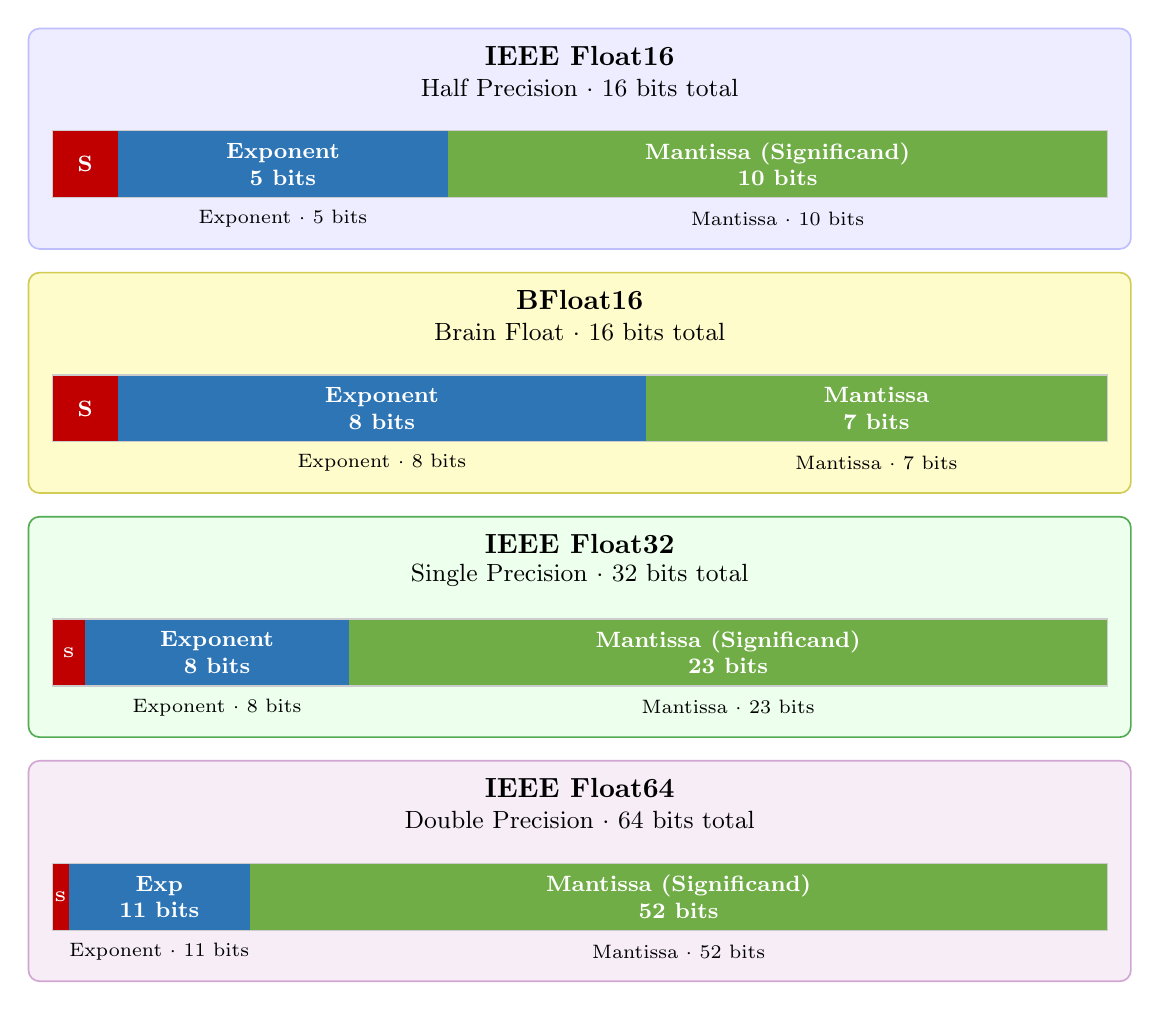
\begin{tikzpicture}[x=1cm, y=1cm]

  % ---- Color palette ----
  \definecolor{signcolor}{RGB}{192,0,0}     % red   -- sign bit
  \definecolor{expcolor} {RGB}{46,117,182}  % blue  -- exponent
  \definecolor{mancolor} {RGB}{112,173,71}  % green -- mantissa

  % ---- Panel backgrounds ----
  % Panels are 14 cm wide x 2.8 cm tall, separated by 0.3 cm gaps.
  % Y positions (bottom edge): Float16=9.30, BFloat16=6.20, Float32=3.10, Float64=0.00
  \draw[rounded corners=4pt, fill=blue!7,    draw=blue!25,        line width=0.6pt]
      (0.0,  9.30) rectangle (14.0, 12.10);  % Float16
  \draw[rounded corners=4pt, fill=yellow!20, draw=yellow!60!gray, line width=0.6pt]
      (0.0,  6.20) rectangle (14.0,  9.00);  % BFloat16
  \draw[rounded corners=4pt, fill=green!7,   draw=green!35!gray,  line width=0.6pt]
      (0.0,  3.10) rectangle (14.0,  5.90);  % Float32
  \draw[rounded corners=4pt, fill=violet!7,  draw=violet!35,      line width=0.6pt]
      (0.0,  0.00) rectangle (14.0,  2.80);  % Float64

  % ====================================================================
  % Bar geometry (shared across all panels):
  %   x range:    [0.30, 13.70]  => total bar width = 13.40 cm
  %   bar height: 0.85 cm
  %   bar bottom: panel_bottom + 0.65
  %   bar top:    panel_bottom + 1.50
  %
  % Segment x boundaries  (width = n_bits/total * 13.40):
  %   Float16  (16-bit): 0.300 | 1.138 | 5.325 | 13.700
  %   BFloat16 (16-bit): 0.300 | 1.138 | 7.838 | 13.700
  %   Float32  (32-bit): 0.300 | 0.719 | 4.069 | 13.700
  %   Float64  (64-bit): 0.300 | 0.509 | 2.813 | 13.700
  % ====================================================================

  % ------------------------------------------------------------------
  % IEEE Float16  (panel bottom y = 9.30)
  % ------------------------------------------------------------------
  \node[font=\normalsize\bfseries] at (7.0, 11.75) {IEEE Float16};
  \node[font=\small]               at (7.0, 11.35) {Half Precision $\cdot$ 16 bits total};

  % S:   1/16 * 13.40 = 0.838 cm   x: 0.300 -- 1.138,  center: 0.719
  \fill[signcolor] (0.300,  9.95) rectangle ( 1.138, 10.80);
  \node[text=white, font=\footnotesize\bfseries] at (0.719, 10.375) {S};

  % Exp: 5/16 * 13.40 = 4.188 cm   x: 1.138 -- 5.325,  center: 3.231
  \fill[expcolor]  (1.138,  9.95) rectangle ( 5.325, 10.80);
  \node[text=white, font=\footnotesize\bfseries, align=center] at (3.231, 10.375)
      {Exponent \\ 5 bits};

  % Man: 10/16 * 13.40 = 8.375 cm  x: 5.325 -- 13.700, center: 9.513
  \fill[mancolor]  (5.325,  9.95) rectangle (13.700, 10.80);
  \node[text=white, font=\footnotesize\bfseries, align=center] at (9.513, 10.375)
      {Mantissa (Significand) \\ 10 bits};

  \draw[black!20, line width=0.4pt] (0.300, 9.95) rectangle (13.700, 10.80);

  \node[font=\scriptsize] at (3.231, 9.68) {Exponent $\cdot$ 5 bits};
  \node[font=\scriptsize] at (9.513, 9.68) {Mantissa $\cdot$ 10 bits};

  % ------------------------------------------------------------------
  % BFloat16  (panel bottom y = 6.20)
  % ------------------------------------------------------------------
  \node[font=\normalsize\bfseries] at (7.0, 8.65) {BFloat16};
  \node[font=\small]               at (7.0, 8.25) {Brain Float $\cdot$ 16 bits total};

  % S:   1/16 * 13.40 = 0.838 cm   x: 0.300 -- 1.138,  center: 0.719
  \fill[signcolor] (0.300,  6.85) rectangle ( 1.138,  7.70);
  \node[text=white, font=\footnotesize\bfseries] at (0.719, 7.275) {S};

  % Exp: 8/16 * 13.40 = 6.700 cm   x: 1.138 -- 7.838,  center: 4.488
  \fill[expcolor]  (1.138,  6.85) rectangle ( 7.838,  7.70);
  \node[text=white, font=\footnotesize\bfseries, align=center] at (4.488, 7.275)
      {Exponent \\ 8 bits};

  % Man: 7/16 * 13.40 = 5.863 cm   x: 7.838 -- 13.700, center: 10.769
  \fill[mancolor]  (7.838,  6.85) rectangle (13.700,  7.70);
  \node[text=white, font=\footnotesize\bfseries, align=center] at (10.769, 7.275)
      {Mantissa \\ 7 bits};

  \draw[black!20, line width=0.4pt] (0.300, 6.85) rectangle (13.700, 7.70);

  \node[font=\scriptsize] at ( 4.488, 6.58) {Exponent $\cdot$ 8 bits};
  \node[font=\scriptsize] at (10.769, 6.58) {Mantissa $\cdot$ 7 bits};

  % ------------------------------------------------------------------
  % IEEE Float32  (panel bottom y = 3.10)
  % ------------------------------------------------------------------
  \node[font=\normalsize\bfseries] at (7.0, 5.55) {IEEE Float32};
  \node[font=\small]               at (7.0, 5.15) {Single Precision $\cdot$ 32 bits total};

  % S:   1/32 * 13.40 = 0.419 cm   x: 0.300 -- 0.719,  center: 0.510
  \fill[signcolor] (0.300,  3.75) rectangle ( 0.719,  4.60);
  \node[text=white, font=\tiny\bfseries] at (0.510, 4.175) {S};

  % Exp: 8/32 * 13.40 = 3.350 cm   x: 0.719 -- 4.069,  center: 2.394
  \fill[expcolor]  (0.719,  3.75) rectangle ( 4.069,  4.60);
  \node[text=white, font=\footnotesize\bfseries, align=center] at (2.394, 4.175)
      {Exponent \\ 8 bits};

  % Man: 23/32 * 13.40 = 9.631 cm  x: 4.069 -- 13.700, center: 8.885
  \fill[mancolor]  (4.069,  3.75) rectangle (13.700,  4.60);
  \node[text=white, font=\footnotesize\bfseries, align=center] at (8.885, 4.175)
      {Mantissa (Significand) \\ 23 bits};

  \draw[black!20, line width=0.4pt] (0.300, 3.75) rectangle (13.700, 4.60);

  \node[font=\scriptsize] at (2.394, 3.48) {Exponent $\cdot$ 8 bits};
  \node[font=\scriptsize] at (8.885, 3.48) {Mantissa $\cdot$ 23 bits};

  % ------------------------------------------------------------------
  % IEEE Float64  (panel bottom y = 0.00)
  % ------------------------------------------------------------------
  \node[font=\normalsize\bfseries] at (7.0, 2.45) {IEEE Float64};
  \node[font=\small]               at (7.0, 2.05) {Double Precision $\cdot$ 64 bits total};

  % S:    1/64 * 13.40 = 0.209 cm  x: 0.300 -- 0.509,  center: 0.405
  \fill[signcolor] (0.300,  0.65) rectangle ( 0.509,  1.50);
  \node[text=white, font=\tiny\bfseries] at (0.405, 1.075) {S};

  % Exp: 11/64 * 13.40 = 2.303 cm  x: 0.509 -- 2.813,  center: 1.661
  \fill[expcolor]  (0.509,  0.65) rectangle ( 2.813,  1.50);
  \node[text=white, font=\footnotesize\bfseries, align=center] at (1.661, 1.075)
      {Exp \\ 11 bits};

  % Man: 52/64 * 13.40 = 10.888 cm x: 2.813 -- 13.700, center: 8.257
  \fill[mancolor]  (2.813,  0.65) rectangle (13.700,  1.50);
  \node[text=white, font=\footnotesize\bfseries, align=center] at (8.257, 1.075)
      {Mantissa (Significand) \\ 52 bits};

  \draw[black!20, line width=0.4pt] (0.300, 0.65) rectangle (13.700, 1.50);

  \node[font=\scriptsize] at (1.661, 0.38) {Exponent $\cdot$ 11 bits};
  \node[font=\scriptsize] at (8.257, 0.38) {Mantissa $\cdot$ 52 bits};

\end{tikzpicture}
}
%
% \resizebox scales everything uniformly — coordinates, line widths,
% and fonts — so the result looks identical regardless of the chosen width.
%
% Recommended figure wrapper (single column):
%   \begin{figure}[t]
%     \centering
%     \resizebox{\columnwidth}{!}{% Floating-point format comparison — single-column stack layout
%
% Required in preamble:
%   \usepackage{tikz}
%
% ---- Scaling -------------------------------------------------------
% The tikzpicture is drawn at its natural size: 14 cm wide x 12.1 cm tall.
% Use \resizebox (from the graphicx package, always loaded in IEEE style)
% to scale it to whatever width you need. The height adjusts automatically.
%
%   Fit to a single text column (~8.8 cm in IEEE two-column):
%     \resizebox{\columnwidth}{!}{\input{float_formats_tikz.tex}}
%
%   Fit to the full page width (~17.8 cm in IEEE two-column):
%     \resizebox{\textwidth}{!}{\input{float_formats_tikz.tex}}
%
%   Fit to an arbitrary fraction of the column width:
%     \resizebox{0.9\columnwidth}{!}{\input{float_formats_tikz.tex}}
%
% \resizebox scales everything uniformly — coordinates, line widths,
% and fonts — so the result looks identical regardless of the chosen width.
%
% Recommended figure wrapper (single column):
%   \begin{figure}[t]
%     \centering
%     \resizebox{\columnwidth}{!}{\input{float_formats_tikz.tex}}
%     \caption{...}
%     \label{fig:float-formats}
%   \end{figure}
% --------------------------------------------------------------------
%
% Layout: 4 panels stacked vertically, each 14 cm x 2.8 cm.
% Bar widths are proportional to actual bit-field widths.
%   Float16:  S=1, Exp=5,  Man=10  (16 bits total)
%   BFloat16: S=1, Exp=8,  Man=7   (16 bits total)
%   Float32:  S=1, Exp=8,  Man=23  (32 bits total)
%   Float64:  S=1, Exp=11, Man=52  (64 bits total)

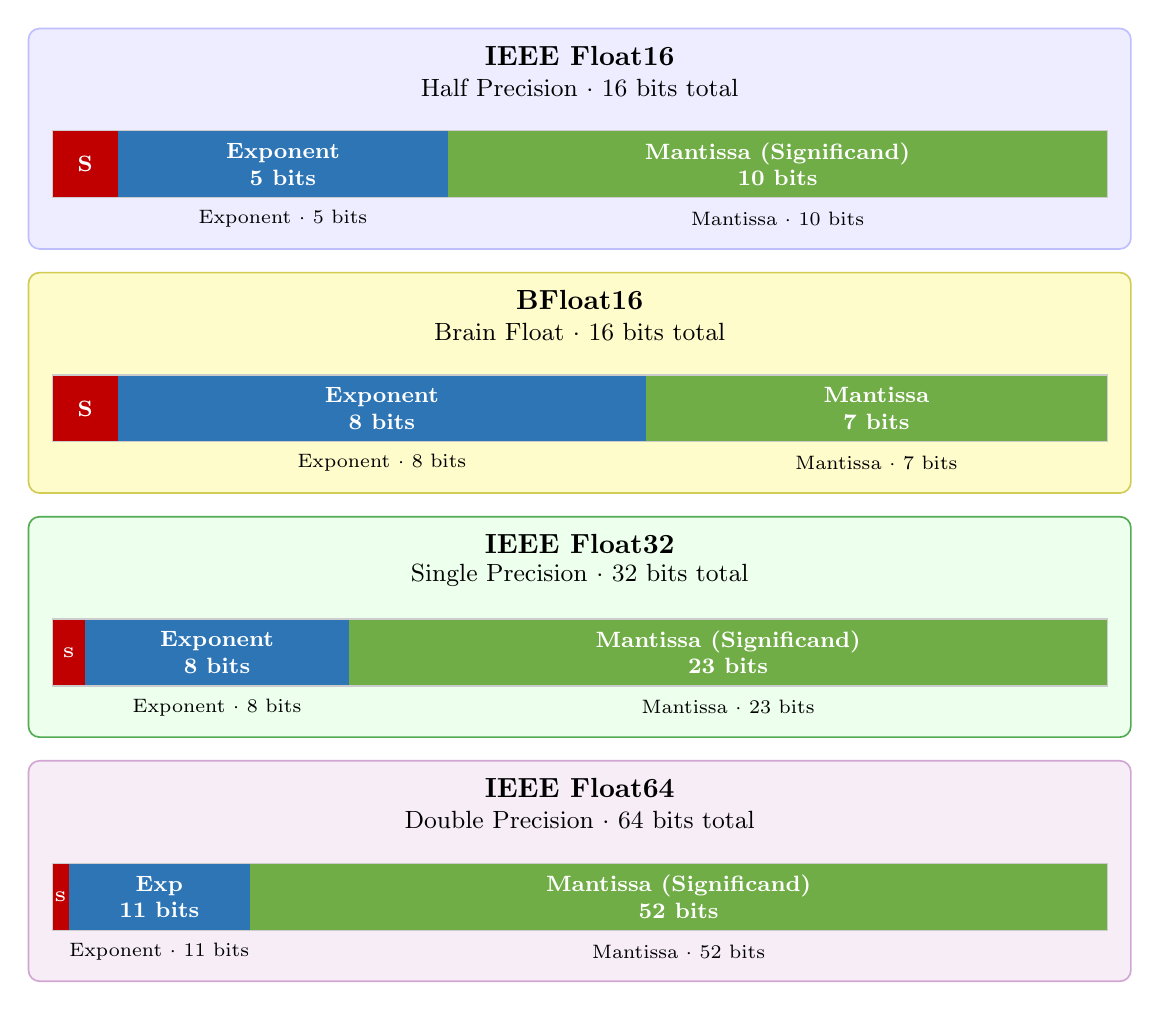
\begin{tikzpicture}[x=1cm, y=1cm]

  % ---- Color palette ----
  \definecolor{signcolor}{RGB}{192,0,0}     % red   -- sign bit
  \definecolor{expcolor} {RGB}{46,117,182}  % blue  -- exponent
  \definecolor{mancolor} {RGB}{112,173,71}  % green -- mantissa

  % ---- Panel backgrounds ----
  % Panels are 14 cm wide x 2.8 cm tall, separated by 0.3 cm gaps.
  % Y positions (bottom edge): Float16=9.30, BFloat16=6.20, Float32=3.10, Float64=0.00
  \draw[rounded corners=4pt, fill=blue!7,    draw=blue!25,        line width=0.6pt]
      (0.0,  9.30) rectangle (14.0, 12.10);  % Float16
  \draw[rounded corners=4pt, fill=yellow!20, draw=yellow!60!gray, line width=0.6pt]
      (0.0,  6.20) rectangle (14.0,  9.00);  % BFloat16
  \draw[rounded corners=4pt, fill=green!7,   draw=green!35!gray,  line width=0.6pt]
      (0.0,  3.10) rectangle (14.0,  5.90);  % Float32
  \draw[rounded corners=4pt, fill=violet!7,  draw=violet!35,      line width=0.6pt]
      (0.0,  0.00) rectangle (14.0,  2.80);  % Float64

  % ====================================================================
  % Bar geometry (shared across all panels):
  %   x range:    [0.30, 13.70]  => total bar width = 13.40 cm
  %   bar height: 0.85 cm
  %   bar bottom: panel_bottom + 0.65
  %   bar top:    panel_bottom + 1.50
  %
  % Segment x boundaries  (width = n_bits/total * 13.40):
  %   Float16  (16-bit): 0.300 | 1.138 | 5.325 | 13.700
  %   BFloat16 (16-bit): 0.300 | 1.138 | 7.838 | 13.700
  %   Float32  (32-bit): 0.300 | 0.719 | 4.069 | 13.700
  %   Float64  (64-bit): 0.300 | 0.509 | 2.813 | 13.700
  % ====================================================================

  % ------------------------------------------------------------------
  % IEEE Float16  (panel bottom y = 9.30)
  % ------------------------------------------------------------------
  \node[font=\normalsize\bfseries] at (7.0, 11.75) {IEEE Float16};
  \node[font=\small]               at (7.0, 11.35) {Half Precision $\cdot$ 16 bits total};

  % S:   1/16 * 13.40 = 0.838 cm   x: 0.300 -- 1.138,  center: 0.719
  \fill[signcolor] (0.300,  9.95) rectangle ( 1.138, 10.80);
  \node[text=white, font=\footnotesize\bfseries] at (0.719, 10.375) {S};

  % Exp: 5/16 * 13.40 = 4.188 cm   x: 1.138 -- 5.325,  center: 3.231
  \fill[expcolor]  (1.138,  9.95) rectangle ( 5.325, 10.80);
  \node[text=white, font=\footnotesize\bfseries, align=center] at (3.231, 10.375)
      {Exponent \\ 5 bits};

  % Man: 10/16 * 13.40 = 8.375 cm  x: 5.325 -- 13.700, center: 9.513
  \fill[mancolor]  (5.325,  9.95) rectangle (13.700, 10.80);
  \node[text=white, font=\footnotesize\bfseries, align=center] at (9.513, 10.375)
      {Mantissa (Significand) \\ 10 bits};

  \draw[black!20, line width=0.4pt] (0.300, 9.95) rectangle (13.700, 10.80);

  \node[font=\scriptsize] at (3.231, 9.68) {Exponent $\cdot$ 5 bits};
  \node[font=\scriptsize] at (9.513, 9.68) {Mantissa $\cdot$ 10 bits};

  % ------------------------------------------------------------------
  % BFloat16  (panel bottom y = 6.20)
  % ------------------------------------------------------------------
  \node[font=\normalsize\bfseries] at (7.0, 8.65) {BFloat16};
  \node[font=\small]               at (7.0, 8.25) {Brain Float $\cdot$ 16 bits total};

  % S:   1/16 * 13.40 = 0.838 cm   x: 0.300 -- 1.138,  center: 0.719
  \fill[signcolor] (0.300,  6.85) rectangle ( 1.138,  7.70);
  \node[text=white, font=\footnotesize\bfseries] at (0.719, 7.275) {S};

  % Exp: 8/16 * 13.40 = 6.700 cm   x: 1.138 -- 7.838,  center: 4.488
  \fill[expcolor]  (1.138,  6.85) rectangle ( 7.838,  7.70);
  \node[text=white, font=\footnotesize\bfseries, align=center] at (4.488, 7.275)
      {Exponent \\ 8 bits};

  % Man: 7/16 * 13.40 = 5.863 cm   x: 7.838 -- 13.700, center: 10.769
  \fill[mancolor]  (7.838,  6.85) rectangle (13.700,  7.70);
  \node[text=white, font=\footnotesize\bfseries, align=center] at (10.769, 7.275)
      {Mantissa \\ 7 bits};

  \draw[black!20, line width=0.4pt] (0.300, 6.85) rectangle (13.700, 7.70);

  \node[font=\scriptsize] at ( 4.488, 6.58) {Exponent $\cdot$ 8 bits};
  \node[font=\scriptsize] at (10.769, 6.58) {Mantissa $\cdot$ 7 bits};

  % ------------------------------------------------------------------
  % IEEE Float32  (panel bottom y = 3.10)
  % ------------------------------------------------------------------
  \node[font=\normalsize\bfseries] at (7.0, 5.55) {IEEE Float32};
  \node[font=\small]               at (7.0, 5.15) {Single Precision $\cdot$ 32 bits total};

  % S:   1/32 * 13.40 = 0.419 cm   x: 0.300 -- 0.719,  center: 0.510
  \fill[signcolor] (0.300,  3.75) rectangle ( 0.719,  4.60);
  \node[text=white, font=\tiny\bfseries] at (0.510, 4.175) {S};

  % Exp: 8/32 * 13.40 = 3.350 cm   x: 0.719 -- 4.069,  center: 2.394
  \fill[expcolor]  (0.719,  3.75) rectangle ( 4.069,  4.60);
  \node[text=white, font=\footnotesize\bfseries, align=center] at (2.394, 4.175)
      {Exponent \\ 8 bits};

  % Man: 23/32 * 13.40 = 9.631 cm  x: 4.069 -- 13.700, center: 8.885
  \fill[mancolor]  (4.069,  3.75) rectangle (13.700,  4.60);
  \node[text=white, font=\footnotesize\bfseries, align=center] at (8.885, 4.175)
      {Mantissa (Significand) \\ 23 bits};

  \draw[black!20, line width=0.4pt] (0.300, 3.75) rectangle (13.700, 4.60);

  \node[font=\scriptsize] at (2.394, 3.48) {Exponent $\cdot$ 8 bits};
  \node[font=\scriptsize] at (8.885, 3.48) {Mantissa $\cdot$ 23 bits};

  % ------------------------------------------------------------------
  % IEEE Float64  (panel bottom y = 0.00)
  % ------------------------------------------------------------------
  \node[font=\normalsize\bfseries] at (7.0, 2.45) {IEEE Float64};
  \node[font=\small]               at (7.0, 2.05) {Double Precision $\cdot$ 64 bits total};

  % S:    1/64 * 13.40 = 0.209 cm  x: 0.300 -- 0.509,  center: 0.405
  \fill[signcolor] (0.300,  0.65) rectangle ( 0.509,  1.50);
  \node[text=white, font=\tiny\bfseries] at (0.405, 1.075) {S};

  % Exp: 11/64 * 13.40 = 2.303 cm  x: 0.509 -- 2.813,  center: 1.661
  \fill[expcolor]  (0.509,  0.65) rectangle ( 2.813,  1.50);
  \node[text=white, font=\footnotesize\bfseries, align=center] at (1.661, 1.075)
      {Exp \\ 11 bits};

  % Man: 52/64 * 13.40 = 10.888 cm x: 2.813 -- 13.700, center: 8.257
  \fill[mancolor]  (2.813,  0.65) rectangle (13.700,  1.50);
  \node[text=white, font=\footnotesize\bfseries, align=center] at (8.257, 1.075)
      {Mantissa (Significand) \\ 52 bits};

  \draw[black!20, line width=0.4pt] (0.300, 0.65) rectangle (13.700, 1.50);

  \node[font=\scriptsize] at (1.661, 0.38) {Exponent $\cdot$ 11 bits};
  \node[font=\scriptsize] at (8.257, 0.38) {Mantissa $\cdot$ 52 bits};

\end{tikzpicture}
}
%     \caption{...}
%     \label{fig:float-formats}
%   \end{figure}
% --------------------------------------------------------------------
%
% Layout: 4 panels stacked vertically, each 14 cm x 2.8 cm.
% Bar widths are proportional to actual bit-field widths.
%   Float16:  S=1, Exp=5,  Man=10  (16 bits total)
%   BFloat16: S=1, Exp=8,  Man=7   (16 bits total)
%   Float32:  S=1, Exp=8,  Man=23  (32 bits total)
%   Float64:  S=1, Exp=11, Man=52  (64 bits total)

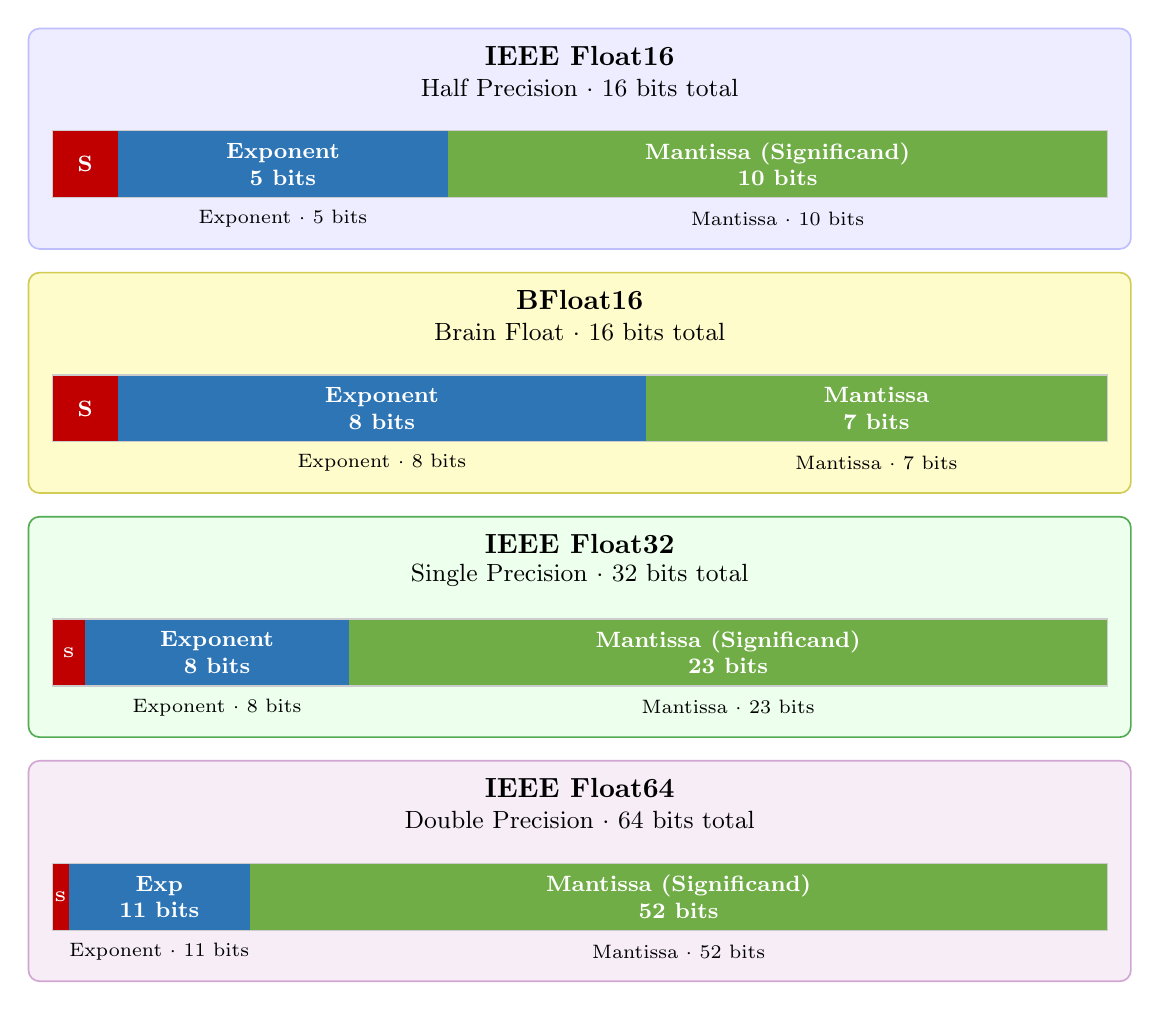
\begin{tikzpicture}[x=1cm, y=1cm]

  % ---- Color palette ----
  \definecolor{signcolor}{RGB}{192,0,0}     % red   -- sign bit
  \definecolor{expcolor} {RGB}{46,117,182}  % blue  -- exponent
  \definecolor{mancolor} {RGB}{112,173,71}  % green -- mantissa

  % ---- Panel backgrounds ----
  % Panels are 14 cm wide x 2.8 cm tall, separated by 0.3 cm gaps.
  % Y positions (bottom edge): Float16=9.30, BFloat16=6.20, Float32=3.10, Float64=0.00
  \draw[rounded corners=4pt, fill=blue!7,    draw=blue!25,        line width=0.6pt]
      (0.0,  9.30) rectangle (14.0, 12.10);  % Float16
  \draw[rounded corners=4pt, fill=yellow!20, draw=yellow!60!gray, line width=0.6pt]
      (0.0,  6.20) rectangle (14.0,  9.00);  % BFloat16
  \draw[rounded corners=4pt, fill=green!7,   draw=green!35!gray,  line width=0.6pt]
      (0.0,  3.10) rectangle (14.0,  5.90);  % Float32
  \draw[rounded corners=4pt, fill=violet!7,  draw=violet!35,      line width=0.6pt]
      (0.0,  0.00) rectangle (14.0,  2.80);  % Float64

  % ====================================================================
  % Bar geometry (shared across all panels):
  %   x range:    [0.30, 13.70]  => total bar width = 13.40 cm
  %   bar height: 0.85 cm
  %   bar bottom: panel_bottom + 0.65
  %   bar top:    panel_bottom + 1.50
  %
  % Segment x boundaries  (width = n_bits/total * 13.40):
  %   Float16  (16-bit): 0.300 | 1.138 | 5.325 | 13.700
  %   BFloat16 (16-bit): 0.300 | 1.138 | 7.838 | 13.700
  %   Float32  (32-bit): 0.300 | 0.719 | 4.069 | 13.700
  %   Float64  (64-bit): 0.300 | 0.509 | 2.813 | 13.700
  % ====================================================================

  % ------------------------------------------------------------------
  % IEEE Float16  (panel bottom y = 9.30)
  % ------------------------------------------------------------------
  \node[font=\normalsize\bfseries] at (7.0, 11.75) {IEEE Float16};
  \node[font=\small]               at (7.0, 11.35) {Half Precision $\cdot$ 16 bits total};

  % S:   1/16 * 13.40 = 0.838 cm   x: 0.300 -- 1.138,  center: 0.719
  \fill[signcolor] (0.300,  9.95) rectangle ( 1.138, 10.80);
  \node[text=white, font=\footnotesize\bfseries] at (0.719, 10.375) {S};

  % Exp: 5/16 * 13.40 = 4.188 cm   x: 1.138 -- 5.325,  center: 3.231
  \fill[expcolor]  (1.138,  9.95) rectangle ( 5.325, 10.80);
  \node[text=white, font=\footnotesize\bfseries, align=center] at (3.231, 10.375)
      {Exponent \\ 5 bits};

  % Man: 10/16 * 13.40 = 8.375 cm  x: 5.325 -- 13.700, center: 9.513
  \fill[mancolor]  (5.325,  9.95) rectangle (13.700, 10.80);
  \node[text=white, font=\footnotesize\bfseries, align=center] at (9.513, 10.375)
      {Mantissa (Significand) \\ 10 bits};

  \draw[black!20, line width=0.4pt] (0.300, 9.95) rectangle (13.700, 10.80);

  \node[font=\scriptsize] at (3.231, 9.68) {Exponent $\cdot$ 5 bits};
  \node[font=\scriptsize] at (9.513, 9.68) {Mantissa $\cdot$ 10 bits};

  % ------------------------------------------------------------------
  % BFloat16  (panel bottom y = 6.20)
  % ------------------------------------------------------------------
  \node[font=\normalsize\bfseries] at (7.0, 8.65) {BFloat16};
  \node[font=\small]               at (7.0, 8.25) {Brain Float $\cdot$ 16 bits total};

  % S:   1/16 * 13.40 = 0.838 cm   x: 0.300 -- 1.138,  center: 0.719
  \fill[signcolor] (0.300,  6.85) rectangle ( 1.138,  7.70);
  \node[text=white, font=\footnotesize\bfseries] at (0.719, 7.275) {S};

  % Exp: 8/16 * 13.40 = 6.700 cm   x: 1.138 -- 7.838,  center: 4.488
  \fill[expcolor]  (1.138,  6.85) rectangle ( 7.838,  7.70);
  \node[text=white, font=\footnotesize\bfseries, align=center] at (4.488, 7.275)
      {Exponent \\ 8 bits};

  % Man: 7/16 * 13.40 = 5.863 cm   x: 7.838 -- 13.700, center: 10.769
  \fill[mancolor]  (7.838,  6.85) rectangle (13.700,  7.70);
  \node[text=white, font=\footnotesize\bfseries, align=center] at (10.769, 7.275)
      {Mantissa \\ 7 bits};

  \draw[black!20, line width=0.4pt] (0.300, 6.85) rectangle (13.700, 7.70);

  \node[font=\scriptsize] at ( 4.488, 6.58) {Exponent $\cdot$ 8 bits};
  \node[font=\scriptsize] at (10.769, 6.58) {Mantissa $\cdot$ 7 bits};

  % ------------------------------------------------------------------
  % IEEE Float32  (panel bottom y = 3.10)
  % ------------------------------------------------------------------
  \node[font=\normalsize\bfseries] at (7.0, 5.55) {IEEE Float32};
  \node[font=\small]               at (7.0, 5.15) {Single Precision $\cdot$ 32 bits total};

  % S:   1/32 * 13.40 = 0.419 cm   x: 0.300 -- 0.719,  center: 0.510
  \fill[signcolor] (0.300,  3.75) rectangle ( 0.719,  4.60);
  \node[text=white, font=\tiny\bfseries] at (0.510, 4.175) {S};

  % Exp: 8/32 * 13.40 = 3.350 cm   x: 0.719 -- 4.069,  center: 2.394
  \fill[expcolor]  (0.719,  3.75) rectangle ( 4.069,  4.60);
  \node[text=white, font=\footnotesize\bfseries, align=center] at (2.394, 4.175)
      {Exponent \\ 8 bits};

  % Man: 23/32 * 13.40 = 9.631 cm  x: 4.069 -- 13.700, center: 8.885
  \fill[mancolor]  (4.069,  3.75) rectangle (13.700,  4.60);
  \node[text=white, font=\footnotesize\bfseries, align=center] at (8.885, 4.175)
      {Mantissa (Significand) \\ 23 bits};

  \draw[black!20, line width=0.4pt] (0.300, 3.75) rectangle (13.700, 4.60);

  \node[font=\scriptsize] at (2.394, 3.48) {Exponent $\cdot$ 8 bits};
  \node[font=\scriptsize] at (8.885, 3.48) {Mantissa $\cdot$ 23 bits};

  % ------------------------------------------------------------------
  % IEEE Float64  (panel bottom y = 0.00)
  % ------------------------------------------------------------------
  \node[font=\normalsize\bfseries] at (7.0, 2.45) {IEEE Float64};
  \node[font=\small]               at (7.0, 2.05) {Double Precision $\cdot$ 64 bits total};

  % S:    1/64 * 13.40 = 0.209 cm  x: 0.300 -- 0.509,  center: 0.405
  \fill[signcolor] (0.300,  0.65) rectangle ( 0.509,  1.50);
  \node[text=white, font=\tiny\bfseries] at (0.405, 1.075) {S};

  % Exp: 11/64 * 13.40 = 2.303 cm  x: 0.509 -- 2.813,  center: 1.661
  \fill[expcolor]  (0.509,  0.65) rectangle ( 2.813,  1.50);
  \node[text=white, font=\footnotesize\bfseries, align=center] at (1.661, 1.075)
      {Exp \\ 11 bits};

  % Man: 52/64 * 13.40 = 10.888 cm x: 2.813 -- 13.700, center: 8.257
  \fill[mancolor]  (2.813,  0.65) rectangle (13.700,  1.50);
  \node[text=white, font=\footnotesize\bfseries, align=center] at (8.257, 1.075)
      {Mantissa (Significand) \\ 52 bits};

  \draw[black!20, line width=0.4pt] (0.300, 0.65) rectangle (13.700, 1.50);

  \node[font=\scriptsize] at (1.661, 0.38) {Exponent $\cdot$ 11 bits};
  \node[font=\scriptsize] at (8.257, 0.38) {Mantissa $\cdot$ 52 bits};

\end{tikzpicture}
}
%
%   Fit to the full page width (~17.8 cm in IEEE two-column):
%     \resizebox{\textwidth}{!}{% Floating-point format comparison — single-column stack layout
%
% Required in preamble:
%   \usepackage{tikz}
%
% ---- Scaling -------------------------------------------------------
% The tikzpicture is drawn at its natural size: 14 cm wide x 12.1 cm tall.
% Use \resizebox (from the graphicx package, always loaded in IEEE style)
% to scale it to whatever width you need. The height adjusts automatically.
%
%   Fit to a single text column (~8.8 cm in IEEE two-column):
%     \resizebox{\columnwidth}{!}{% Floating-point format comparison — single-column stack layout
%
% Required in preamble:
%   \usepackage{tikz}
%
% ---- Scaling -------------------------------------------------------
% The tikzpicture is drawn at its natural size: 14 cm wide x 12.1 cm tall.
% Use \resizebox (from the graphicx package, always loaded in IEEE style)
% to scale it to whatever width you need. The height adjusts automatically.
%
%   Fit to a single text column (~8.8 cm in IEEE two-column):
%     \resizebox{\columnwidth}{!}{\input{float_formats_tikz.tex}}
%
%   Fit to the full page width (~17.8 cm in IEEE two-column):
%     \resizebox{\textwidth}{!}{\input{float_formats_tikz.tex}}
%
%   Fit to an arbitrary fraction of the column width:
%     \resizebox{0.9\columnwidth}{!}{\input{float_formats_tikz.tex}}
%
% \resizebox scales everything uniformly — coordinates, line widths,
% and fonts — so the result looks identical regardless of the chosen width.
%
% Recommended figure wrapper (single column):
%   \begin{figure}[t]
%     \centering
%     \resizebox{\columnwidth}{!}{\input{float_formats_tikz.tex}}
%     \caption{...}
%     \label{fig:float-formats}
%   \end{figure}
% --------------------------------------------------------------------
%
% Layout: 4 panels stacked vertically, each 14 cm x 2.8 cm.
% Bar widths are proportional to actual bit-field widths.
%   Float16:  S=1, Exp=5,  Man=10  (16 bits total)
%   BFloat16: S=1, Exp=8,  Man=7   (16 bits total)
%   Float32:  S=1, Exp=8,  Man=23  (32 bits total)
%   Float64:  S=1, Exp=11, Man=52  (64 bits total)

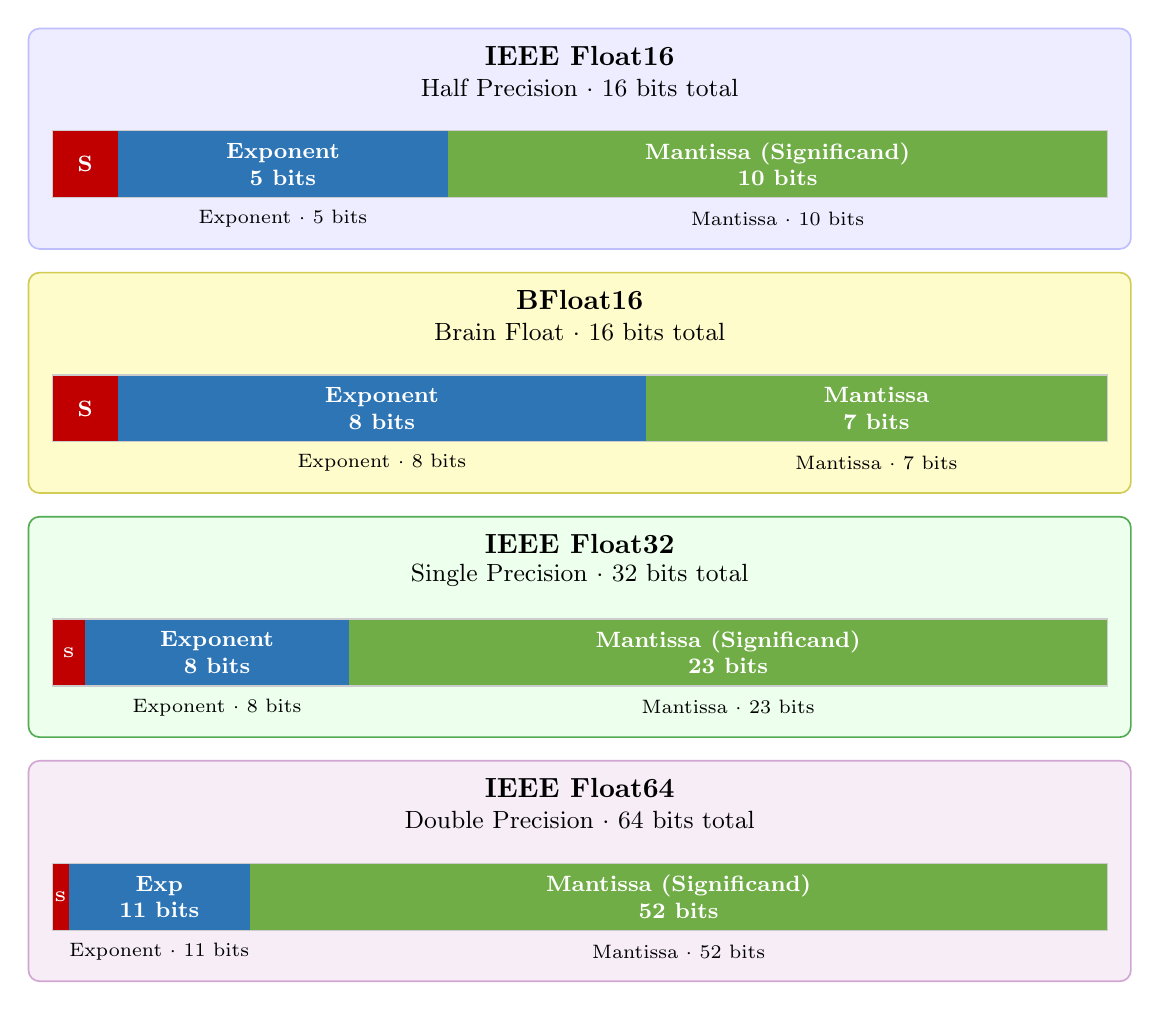
\begin{tikzpicture}[x=1cm, y=1cm]

  % ---- Color palette ----
  \definecolor{signcolor}{RGB}{192,0,0}     % red   -- sign bit
  \definecolor{expcolor} {RGB}{46,117,182}  % blue  -- exponent
  \definecolor{mancolor} {RGB}{112,173,71}  % green -- mantissa

  % ---- Panel backgrounds ----
  % Panels are 14 cm wide x 2.8 cm tall, separated by 0.3 cm gaps.
  % Y positions (bottom edge): Float16=9.30, BFloat16=6.20, Float32=3.10, Float64=0.00
  \draw[rounded corners=4pt, fill=blue!7,    draw=blue!25,        line width=0.6pt]
      (0.0,  9.30) rectangle (14.0, 12.10);  % Float16
  \draw[rounded corners=4pt, fill=yellow!20, draw=yellow!60!gray, line width=0.6pt]
      (0.0,  6.20) rectangle (14.0,  9.00);  % BFloat16
  \draw[rounded corners=4pt, fill=green!7,   draw=green!35!gray,  line width=0.6pt]
      (0.0,  3.10) rectangle (14.0,  5.90);  % Float32
  \draw[rounded corners=4pt, fill=violet!7,  draw=violet!35,      line width=0.6pt]
      (0.0,  0.00) rectangle (14.0,  2.80);  % Float64

  % ====================================================================
  % Bar geometry (shared across all panels):
  %   x range:    [0.30, 13.70]  => total bar width = 13.40 cm
  %   bar height: 0.85 cm
  %   bar bottom: panel_bottom + 0.65
  %   bar top:    panel_bottom + 1.50
  %
  % Segment x boundaries  (width = n_bits/total * 13.40):
  %   Float16  (16-bit): 0.300 | 1.138 | 5.325 | 13.700
  %   BFloat16 (16-bit): 0.300 | 1.138 | 7.838 | 13.700
  %   Float32  (32-bit): 0.300 | 0.719 | 4.069 | 13.700
  %   Float64  (64-bit): 0.300 | 0.509 | 2.813 | 13.700
  % ====================================================================

  % ------------------------------------------------------------------
  % IEEE Float16  (panel bottom y = 9.30)
  % ------------------------------------------------------------------
  \node[font=\normalsize\bfseries] at (7.0, 11.75) {IEEE Float16};
  \node[font=\small]               at (7.0, 11.35) {Half Precision $\cdot$ 16 bits total};

  % S:   1/16 * 13.40 = 0.838 cm   x: 0.300 -- 1.138,  center: 0.719
  \fill[signcolor] (0.300,  9.95) rectangle ( 1.138, 10.80);
  \node[text=white, font=\footnotesize\bfseries] at (0.719, 10.375) {S};

  % Exp: 5/16 * 13.40 = 4.188 cm   x: 1.138 -- 5.325,  center: 3.231
  \fill[expcolor]  (1.138,  9.95) rectangle ( 5.325, 10.80);
  \node[text=white, font=\footnotesize\bfseries, align=center] at (3.231, 10.375)
      {Exponent \\ 5 bits};

  % Man: 10/16 * 13.40 = 8.375 cm  x: 5.325 -- 13.700, center: 9.513
  \fill[mancolor]  (5.325,  9.95) rectangle (13.700, 10.80);
  \node[text=white, font=\footnotesize\bfseries, align=center] at (9.513, 10.375)
      {Mantissa (Significand) \\ 10 bits};

  \draw[black!20, line width=0.4pt] (0.300, 9.95) rectangle (13.700, 10.80);

  \node[font=\scriptsize] at (3.231, 9.68) {Exponent $\cdot$ 5 bits};
  \node[font=\scriptsize] at (9.513, 9.68) {Mantissa $\cdot$ 10 bits};

  % ------------------------------------------------------------------
  % BFloat16  (panel bottom y = 6.20)
  % ------------------------------------------------------------------
  \node[font=\normalsize\bfseries] at (7.0, 8.65) {BFloat16};
  \node[font=\small]               at (7.0, 8.25) {Brain Float $\cdot$ 16 bits total};

  % S:   1/16 * 13.40 = 0.838 cm   x: 0.300 -- 1.138,  center: 0.719
  \fill[signcolor] (0.300,  6.85) rectangle ( 1.138,  7.70);
  \node[text=white, font=\footnotesize\bfseries] at (0.719, 7.275) {S};

  % Exp: 8/16 * 13.40 = 6.700 cm   x: 1.138 -- 7.838,  center: 4.488
  \fill[expcolor]  (1.138,  6.85) rectangle ( 7.838,  7.70);
  \node[text=white, font=\footnotesize\bfseries, align=center] at (4.488, 7.275)
      {Exponent \\ 8 bits};

  % Man: 7/16 * 13.40 = 5.863 cm   x: 7.838 -- 13.700, center: 10.769
  \fill[mancolor]  (7.838,  6.85) rectangle (13.700,  7.70);
  \node[text=white, font=\footnotesize\bfseries, align=center] at (10.769, 7.275)
      {Mantissa \\ 7 bits};

  \draw[black!20, line width=0.4pt] (0.300, 6.85) rectangle (13.700, 7.70);

  \node[font=\scriptsize] at ( 4.488, 6.58) {Exponent $\cdot$ 8 bits};
  \node[font=\scriptsize] at (10.769, 6.58) {Mantissa $\cdot$ 7 bits};

  % ------------------------------------------------------------------
  % IEEE Float32  (panel bottom y = 3.10)
  % ------------------------------------------------------------------
  \node[font=\normalsize\bfseries] at (7.0, 5.55) {IEEE Float32};
  \node[font=\small]               at (7.0, 5.15) {Single Precision $\cdot$ 32 bits total};

  % S:   1/32 * 13.40 = 0.419 cm   x: 0.300 -- 0.719,  center: 0.510
  \fill[signcolor] (0.300,  3.75) rectangle ( 0.719,  4.60);
  \node[text=white, font=\tiny\bfseries] at (0.510, 4.175) {S};

  % Exp: 8/32 * 13.40 = 3.350 cm   x: 0.719 -- 4.069,  center: 2.394
  \fill[expcolor]  (0.719,  3.75) rectangle ( 4.069,  4.60);
  \node[text=white, font=\footnotesize\bfseries, align=center] at (2.394, 4.175)
      {Exponent \\ 8 bits};

  % Man: 23/32 * 13.40 = 9.631 cm  x: 4.069 -- 13.700, center: 8.885
  \fill[mancolor]  (4.069,  3.75) rectangle (13.700,  4.60);
  \node[text=white, font=\footnotesize\bfseries, align=center] at (8.885, 4.175)
      {Mantissa (Significand) \\ 23 bits};

  \draw[black!20, line width=0.4pt] (0.300, 3.75) rectangle (13.700, 4.60);

  \node[font=\scriptsize] at (2.394, 3.48) {Exponent $\cdot$ 8 bits};
  \node[font=\scriptsize] at (8.885, 3.48) {Mantissa $\cdot$ 23 bits};

  % ------------------------------------------------------------------
  % IEEE Float64  (panel bottom y = 0.00)
  % ------------------------------------------------------------------
  \node[font=\normalsize\bfseries] at (7.0, 2.45) {IEEE Float64};
  \node[font=\small]               at (7.0, 2.05) {Double Precision $\cdot$ 64 bits total};

  % S:    1/64 * 13.40 = 0.209 cm  x: 0.300 -- 0.509,  center: 0.405
  \fill[signcolor] (0.300,  0.65) rectangle ( 0.509,  1.50);
  \node[text=white, font=\tiny\bfseries] at (0.405, 1.075) {S};

  % Exp: 11/64 * 13.40 = 2.303 cm  x: 0.509 -- 2.813,  center: 1.661
  \fill[expcolor]  (0.509,  0.65) rectangle ( 2.813,  1.50);
  \node[text=white, font=\footnotesize\bfseries, align=center] at (1.661, 1.075)
      {Exp \\ 11 bits};

  % Man: 52/64 * 13.40 = 10.888 cm x: 2.813 -- 13.700, center: 8.257
  \fill[mancolor]  (2.813,  0.65) rectangle (13.700,  1.50);
  \node[text=white, font=\footnotesize\bfseries, align=center] at (8.257, 1.075)
      {Mantissa (Significand) \\ 52 bits};

  \draw[black!20, line width=0.4pt] (0.300, 0.65) rectangle (13.700, 1.50);

  \node[font=\scriptsize] at (1.661, 0.38) {Exponent $\cdot$ 11 bits};
  \node[font=\scriptsize] at (8.257, 0.38) {Mantissa $\cdot$ 52 bits};

\end{tikzpicture}
}
%
%   Fit to the full page width (~17.8 cm in IEEE two-column):
%     \resizebox{\textwidth}{!}{% Floating-point format comparison — single-column stack layout
%
% Required in preamble:
%   \usepackage{tikz}
%
% ---- Scaling -------------------------------------------------------
% The tikzpicture is drawn at its natural size: 14 cm wide x 12.1 cm tall.
% Use \resizebox (from the graphicx package, always loaded in IEEE style)
% to scale it to whatever width you need. The height adjusts automatically.
%
%   Fit to a single text column (~8.8 cm in IEEE two-column):
%     \resizebox{\columnwidth}{!}{\input{float_formats_tikz.tex}}
%
%   Fit to the full page width (~17.8 cm in IEEE two-column):
%     \resizebox{\textwidth}{!}{\input{float_formats_tikz.tex}}
%
%   Fit to an arbitrary fraction of the column width:
%     \resizebox{0.9\columnwidth}{!}{\input{float_formats_tikz.tex}}
%
% \resizebox scales everything uniformly — coordinates, line widths,
% and fonts — so the result looks identical regardless of the chosen width.
%
% Recommended figure wrapper (single column):
%   \begin{figure}[t]
%     \centering
%     \resizebox{\columnwidth}{!}{\input{float_formats_tikz.tex}}
%     \caption{...}
%     \label{fig:float-formats}
%   \end{figure}
% --------------------------------------------------------------------
%
% Layout: 4 panels stacked vertically, each 14 cm x 2.8 cm.
% Bar widths are proportional to actual bit-field widths.
%   Float16:  S=1, Exp=5,  Man=10  (16 bits total)
%   BFloat16: S=1, Exp=8,  Man=7   (16 bits total)
%   Float32:  S=1, Exp=8,  Man=23  (32 bits total)
%   Float64:  S=1, Exp=11, Man=52  (64 bits total)

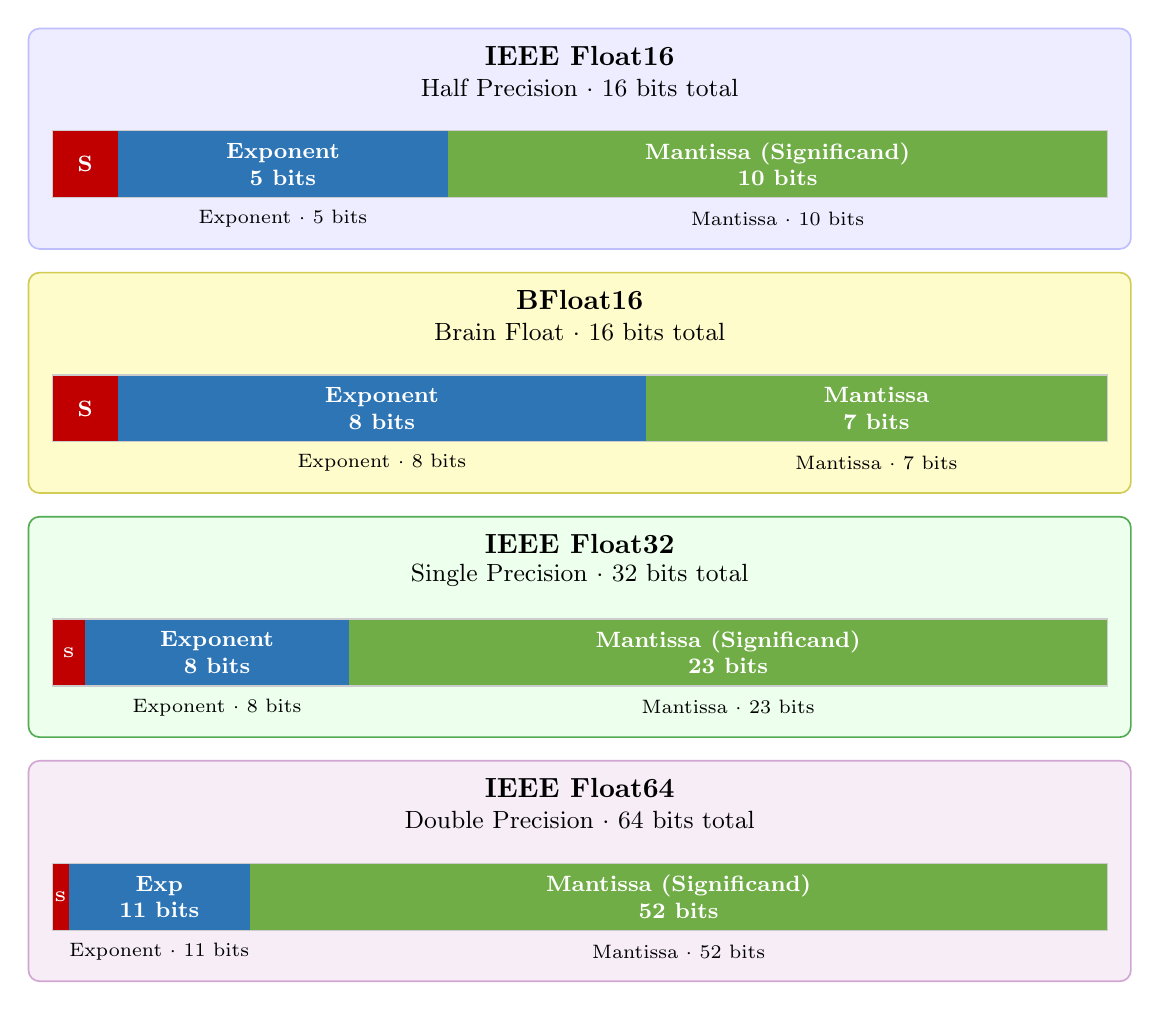
\begin{tikzpicture}[x=1cm, y=1cm]

  % ---- Color palette ----
  \definecolor{signcolor}{RGB}{192,0,0}     % red   -- sign bit
  \definecolor{expcolor} {RGB}{46,117,182}  % blue  -- exponent
  \definecolor{mancolor} {RGB}{112,173,71}  % green -- mantissa

  % ---- Panel backgrounds ----
  % Panels are 14 cm wide x 2.8 cm tall, separated by 0.3 cm gaps.
  % Y positions (bottom edge): Float16=9.30, BFloat16=6.20, Float32=3.10, Float64=0.00
  \draw[rounded corners=4pt, fill=blue!7,    draw=blue!25,        line width=0.6pt]
      (0.0,  9.30) rectangle (14.0, 12.10);  % Float16
  \draw[rounded corners=4pt, fill=yellow!20, draw=yellow!60!gray, line width=0.6pt]
      (0.0,  6.20) rectangle (14.0,  9.00);  % BFloat16
  \draw[rounded corners=4pt, fill=green!7,   draw=green!35!gray,  line width=0.6pt]
      (0.0,  3.10) rectangle (14.0,  5.90);  % Float32
  \draw[rounded corners=4pt, fill=violet!7,  draw=violet!35,      line width=0.6pt]
      (0.0,  0.00) rectangle (14.0,  2.80);  % Float64

  % ====================================================================
  % Bar geometry (shared across all panels):
  %   x range:    [0.30, 13.70]  => total bar width = 13.40 cm
  %   bar height: 0.85 cm
  %   bar bottom: panel_bottom + 0.65
  %   bar top:    panel_bottom + 1.50
  %
  % Segment x boundaries  (width = n_bits/total * 13.40):
  %   Float16  (16-bit): 0.300 | 1.138 | 5.325 | 13.700
  %   BFloat16 (16-bit): 0.300 | 1.138 | 7.838 | 13.700
  %   Float32  (32-bit): 0.300 | 0.719 | 4.069 | 13.700
  %   Float64  (64-bit): 0.300 | 0.509 | 2.813 | 13.700
  % ====================================================================

  % ------------------------------------------------------------------
  % IEEE Float16  (panel bottom y = 9.30)
  % ------------------------------------------------------------------
  \node[font=\normalsize\bfseries] at (7.0, 11.75) {IEEE Float16};
  \node[font=\small]               at (7.0, 11.35) {Half Precision $\cdot$ 16 bits total};

  % S:   1/16 * 13.40 = 0.838 cm   x: 0.300 -- 1.138,  center: 0.719
  \fill[signcolor] (0.300,  9.95) rectangle ( 1.138, 10.80);
  \node[text=white, font=\footnotesize\bfseries] at (0.719, 10.375) {S};

  % Exp: 5/16 * 13.40 = 4.188 cm   x: 1.138 -- 5.325,  center: 3.231
  \fill[expcolor]  (1.138,  9.95) rectangle ( 5.325, 10.80);
  \node[text=white, font=\footnotesize\bfseries, align=center] at (3.231, 10.375)
      {Exponent \\ 5 bits};

  % Man: 10/16 * 13.40 = 8.375 cm  x: 5.325 -- 13.700, center: 9.513
  \fill[mancolor]  (5.325,  9.95) rectangle (13.700, 10.80);
  \node[text=white, font=\footnotesize\bfseries, align=center] at (9.513, 10.375)
      {Mantissa (Significand) \\ 10 bits};

  \draw[black!20, line width=0.4pt] (0.300, 9.95) rectangle (13.700, 10.80);

  \node[font=\scriptsize] at (3.231, 9.68) {Exponent $\cdot$ 5 bits};
  \node[font=\scriptsize] at (9.513, 9.68) {Mantissa $\cdot$ 10 bits};

  % ------------------------------------------------------------------
  % BFloat16  (panel bottom y = 6.20)
  % ------------------------------------------------------------------
  \node[font=\normalsize\bfseries] at (7.0, 8.65) {BFloat16};
  \node[font=\small]               at (7.0, 8.25) {Brain Float $\cdot$ 16 bits total};

  % S:   1/16 * 13.40 = 0.838 cm   x: 0.300 -- 1.138,  center: 0.719
  \fill[signcolor] (0.300,  6.85) rectangle ( 1.138,  7.70);
  \node[text=white, font=\footnotesize\bfseries] at (0.719, 7.275) {S};

  % Exp: 8/16 * 13.40 = 6.700 cm   x: 1.138 -- 7.838,  center: 4.488
  \fill[expcolor]  (1.138,  6.85) rectangle ( 7.838,  7.70);
  \node[text=white, font=\footnotesize\bfseries, align=center] at (4.488, 7.275)
      {Exponent \\ 8 bits};

  % Man: 7/16 * 13.40 = 5.863 cm   x: 7.838 -- 13.700, center: 10.769
  \fill[mancolor]  (7.838,  6.85) rectangle (13.700,  7.70);
  \node[text=white, font=\footnotesize\bfseries, align=center] at (10.769, 7.275)
      {Mantissa \\ 7 bits};

  \draw[black!20, line width=0.4pt] (0.300, 6.85) rectangle (13.700, 7.70);

  \node[font=\scriptsize] at ( 4.488, 6.58) {Exponent $\cdot$ 8 bits};
  \node[font=\scriptsize] at (10.769, 6.58) {Mantissa $\cdot$ 7 bits};

  % ------------------------------------------------------------------
  % IEEE Float32  (panel bottom y = 3.10)
  % ------------------------------------------------------------------
  \node[font=\normalsize\bfseries] at (7.0, 5.55) {IEEE Float32};
  \node[font=\small]               at (7.0, 5.15) {Single Precision $\cdot$ 32 bits total};

  % S:   1/32 * 13.40 = 0.419 cm   x: 0.300 -- 0.719,  center: 0.510
  \fill[signcolor] (0.300,  3.75) rectangle ( 0.719,  4.60);
  \node[text=white, font=\tiny\bfseries] at (0.510, 4.175) {S};

  % Exp: 8/32 * 13.40 = 3.350 cm   x: 0.719 -- 4.069,  center: 2.394
  \fill[expcolor]  (0.719,  3.75) rectangle ( 4.069,  4.60);
  \node[text=white, font=\footnotesize\bfseries, align=center] at (2.394, 4.175)
      {Exponent \\ 8 bits};

  % Man: 23/32 * 13.40 = 9.631 cm  x: 4.069 -- 13.700, center: 8.885
  \fill[mancolor]  (4.069,  3.75) rectangle (13.700,  4.60);
  \node[text=white, font=\footnotesize\bfseries, align=center] at (8.885, 4.175)
      {Mantissa (Significand) \\ 23 bits};

  \draw[black!20, line width=0.4pt] (0.300, 3.75) rectangle (13.700, 4.60);

  \node[font=\scriptsize] at (2.394, 3.48) {Exponent $\cdot$ 8 bits};
  \node[font=\scriptsize] at (8.885, 3.48) {Mantissa $\cdot$ 23 bits};

  % ------------------------------------------------------------------
  % IEEE Float64  (panel bottom y = 0.00)
  % ------------------------------------------------------------------
  \node[font=\normalsize\bfseries] at (7.0, 2.45) {IEEE Float64};
  \node[font=\small]               at (7.0, 2.05) {Double Precision $\cdot$ 64 bits total};

  % S:    1/64 * 13.40 = 0.209 cm  x: 0.300 -- 0.509,  center: 0.405
  \fill[signcolor] (0.300,  0.65) rectangle ( 0.509,  1.50);
  \node[text=white, font=\tiny\bfseries] at (0.405, 1.075) {S};

  % Exp: 11/64 * 13.40 = 2.303 cm  x: 0.509 -- 2.813,  center: 1.661
  \fill[expcolor]  (0.509,  0.65) rectangle ( 2.813,  1.50);
  \node[text=white, font=\footnotesize\bfseries, align=center] at (1.661, 1.075)
      {Exp \\ 11 bits};

  % Man: 52/64 * 13.40 = 10.888 cm x: 2.813 -- 13.700, center: 8.257
  \fill[mancolor]  (2.813,  0.65) rectangle (13.700,  1.50);
  \node[text=white, font=\footnotesize\bfseries, align=center] at (8.257, 1.075)
      {Mantissa (Significand) \\ 52 bits};

  \draw[black!20, line width=0.4pt] (0.300, 0.65) rectangle (13.700, 1.50);

  \node[font=\scriptsize] at (1.661, 0.38) {Exponent $\cdot$ 11 bits};
  \node[font=\scriptsize] at (8.257, 0.38) {Mantissa $\cdot$ 52 bits};

\end{tikzpicture}
}
%
%   Fit to an arbitrary fraction of the column width:
%     \resizebox{0.9\columnwidth}{!}{% Floating-point format comparison — single-column stack layout
%
% Required in preamble:
%   \usepackage{tikz}
%
% ---- Scaling -------------------------------------------------------
% The tikzpicture is drawn at its natural size: 14 cm wide x 12.1 cm tall.
% Use \resizebox (from the graphicx package, always loaded in IEEE style)
% to scale it to whatever width you need. The height adjusts automatically.
%
%   Fit to a single text column (~8.8 cm in IEEE two-column):
%     \resizebox{\columnwidth}{!}{\input{float_formats_tikz.tex}}
%
%   Fit to the full page width (~17.8 cm in IEEE two-column):
%     \resizebox{\textwidth}{!}{\input{float_formats_tikz.tex}}
%
%   Fit to an arbitrary fraction of the column width:
%     \resizebox{0.9\columnwidth}{!}{\input{float_formats_tikz.tex}}
%
% \resizebox scales everything uniformly — coordinates, line widths,
% and fonts — so the result looks identical regardless of the chosen width.
%
% Recommended figure wrapper (single column):
%   \begin{figure}[t]
%     \centering
%     \resizebox{\columnwidth}{!}{\input{float_formats_tikz.tex}}
%     \caption{...}
%     \label{fig:float-formats}
%   \end{figure}
% --------------------------------------------------------------------
%
% Layout: 4 panels stacked vertically, each 14 cm x 2.8 cm.
% Bar widths are proportional to actual bit-field widths.
%   Float16:  S=1, Exp=5,  Man=10  (16 bits total)
%   BFloat16: S=1, Exp=8,  Man=7   (16 bits total)
%   Float32:  S=1, Exp=8,  Man=23  (32 bits total)
%   Float64:  S=1, Exp=11, Man=52  (64 bits total)

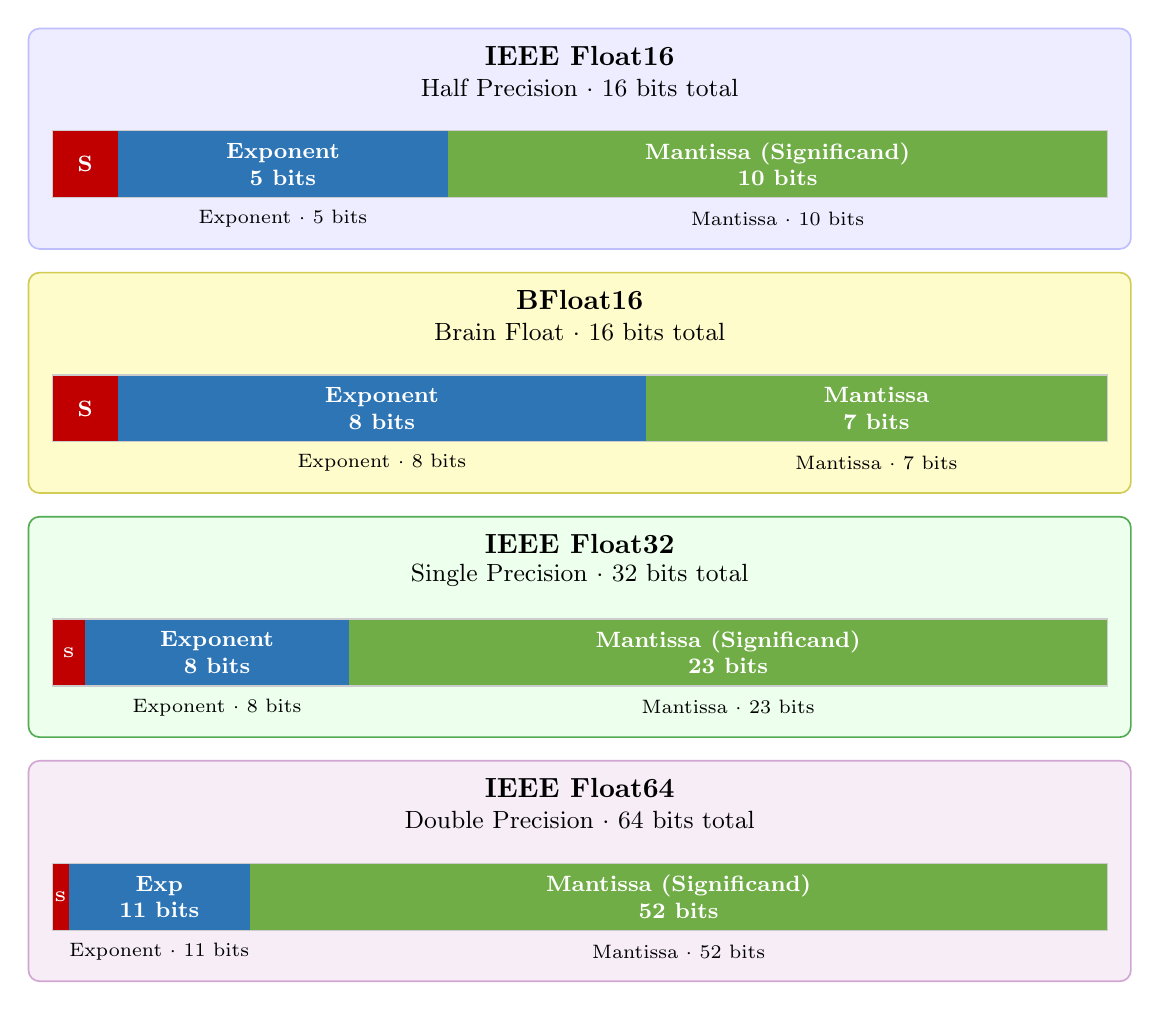
\begin{tikzpicture}[x=1cm, y=1cm]

  % ---- Color palette ----
  \definecolor{signcolor}{RGB}{192,0,0}     % red   -- sign bit
  \definecolor{expcolor} {RGB}{46,117,182}  % blue  -- exponent
  \definecolor{mancolor} {RGB}{112,173,71}  % green -- mantissa

  % ---- Panel backgrounds ----
  % Panels are 14 cm wide x 2.8 cm tall, separated by 0.3 cm gaps.
  % Y positions (bottom edge): Float16=9.30, BFloat16=6.20, Float32=3.10, Float64=0.00
  \draw[rounded corners=4pt, fill=blue!7,    draw=blue!25,        line width=0.6pt]
      (0.0,  9.30) rectangle (14.0, 12.10);  % Float16
  \draw[rounded corners=4pt, fill=yellow!20, draw=yellow!60!gray, line width=0.6pt]
      (0.0,  6.20) rectangle (14.0,  9.00);  % BFloat16
  \draw[rounded corners=4pt, fill=green!7,   draw=green!35!gray,  line width=0.6pt]
      (0.0,  3.10) rectangle (14.0,  5.90);  % Float32
  \draw[rounded corners=4pt, fill=violet!7,  draw=violet!35,      line width=0.6pt]
      (0.0,  0.00) rectangle (14.0,  2.80);  % Float64

  % ====================================================================
  % Bar geometry (shared across all panels):
  %   x range:    [0.30, 13.70]  => total bar width = 13.40 cm
  %   bar height: 0.85 cm
  %   bar bottom: panel_bottom + 0.65
  %   bar top:    panel_bottom + 1.50
  %
  % Segment x boundaries  (width = n_bits/total * 13.40):
  %   Float16  (16-bit): 0.300 | 1.138 | 5.325 | 13.700
  %   BFloat16 (16-bit): 0.300 | 1.138 | 7.838 | 13.700
  %   Float32  (32-bit): 0.300 | 0.719 | 4.069 | 13.700
  %   Float64  (64-bit): 0.300 | 0.509 | 2.813 | 13.700
  % ====================================================================

  % ------------------------------------------------------------------
  % IEEE Float16  (panel bottom y = 9.30)
  % ------------------------------------------------------------------
  \node[font=\normalsize\bfseries] at (7.0, 11.75) {IEEE Float16};
  \node[font=\small]               at (7.0, 11.35) {Half Precision $\cdot$ 16 bits total};

  % S:   1/16 * 13.40 = 0.838 cm   x: 0.300 -- 1.138,  center: 0.719
  \fill[signcolor] (0.300,  9.95) rectangle ( 1.138, 10.80);
  \node[text=white, font=\footnotesize\bfseries] at (0.719, 10.375) {S};

  % Exp: 5/16 * 13.40 = 4.188 cm   x: 1.138 -- 5.325,  center: 3.231
  \fill[expcolor]  (1.138,  9.95) rectangle ( 5.325, 10.80);
  \node[text=white, font=\footnotesize\bfseries, align=center] at (3.231, 10.375)
      {Exponent \\ 5 bits};

  % Man: 10/16 * 13.40 = 8.375 cm  x: 5.325 -- 13.700, center: 9.513
  \fill[mancolor]  (5.325,  9.95) rectangle (13.700, 10.80);
  \node[text=white, font=\footnotesize\bfseries, align=center] at (9.513, 10.375)
      {Mantissa (Significand) \\ 10 bits};

  \draw[black!20, line width=0.4pt] (0.300, 9.95) rectangle (13.700, 10.80);

  \node[font=\scriptsize] at (3.231, 9.68) {Exponent $\cdot$ 5 bits};
  \node[font=\scriptsize] at (9.513, 9.68) {Mantissa $\cdot$ 10 bits};

  % ------------------------------------------------------------------
  % BFloat16  (panel bottom y = 6.20)
  % ------------------------------------------------------------------
  \node[font=\normalsize\bfseries] at (7.0, 8.65) {BFloat16};
  \node[font=\small]               at (7.0, 8.25) {Brain Float $\cdot$ 16 bits total};

  % S:   1/16 * 13.40 = 0.838 cm   x: 0.300 -- 1.138,  center: 0.719
  \fill[signcolor] (0.300,  6.85) rectangle ( 1.138,  7.70);
  \node[text=white, font=\footnotesize\bfseries] at (0.719, 7.275) {S};

  % Exp: 8/16 * 13.40 = 6.700 cm   x: 1.138 -- 7.838,  center: 4.488
  \fill[expcolor]  (1.138,  6.85) rectangle ( 7.838,  7.70);
  \node[text=white, font=\footnotesize\bfseries, align=center] at (4.488, 7.275)
      {Exponent \\ 8 bits};

  % Man: 7/16 * 13.40 = 5.863 cm   x: 7.838 -- 13.700, center: 10.769
  \fill[mancolor]  (7.838,  6.85) rectangle (13.700,  7.70);
  \node[text=white, font=\footnotesize\bfseries, align=center] at (10.769, 7.275)
      {Mantissa \\ 7 bits};

  \draw[black!20, line width=0.4pt] (0.300, 6.85) rectangle (13.700, 7.70);

  \node[font=\scriptsize] at ( 4.488, 6.58) {Exponent $\cdot$ 8 bits};
  \node[font=\scriptsize] at (10.769, 6.58) {Mantissa $\cdot$ 7 bits};

  % ------------------------------------------------------------------
  % IEEE Float32  (panel bottom y = 3.10)
  % ------------------------------------------------------------------
  \node[font=\normalsize\bfseries] at (7.0, 5.55) {IEEE Float32};
  \node[font=\small]               at (7.0, 5.15) {Single Precision $\cdot$ 32 bits total};

  % S:   1/32 * 13.40 = 0.419 cm   x: 0.300 -- 0.719,  center: 0.510
  \fill[signcolor] (0.300,  3.75) rectangle ( 0.719,  4.60);
  \node[text=white, font=\tiny\bfseries] at (0.510, 4.175) {S};

  % Exp: 8/32 * 13.40 = 3.350 cm   x: 0.719 -- 4.069,  center: 2.394
  \fill[expcolor]  (0.719,  3.75) rectangle ( 4.069,  4.60);
  \node[text=white, font=\footnotesize\bfseries, align=center] at (2.394, 4.175)
      {Exponent \\ 8 bits};

  % Man: 23/32 * 13.40 = 9.631 cm  x: 4.069 -- 13.700, center: 8.885
  \fill[mancolor]  (4.069,  3.75) rectangle (13.700,  4.60);
  \node[text=white, font=\footnotesize\bfseries, align=center] at (8.885, 4.175)
      {Mantissa (Significand) \\ 23 bits};

  \draw[black!20, line width=0.4pt] (0.300, 3.75) rectangle (13.700, 4.60);

  \node[font=\scriptsize] at (2.394, 3.48) {Exponent $\cdot$ 8 bits};
  \node[font=\scriptsize] at (8.885, 3.48) {Mantissa $\cdot$ 23 bits};

  % ------------------------------------------------------------------
  % IEEE Float64  (panel bottom y = 0.00)
  % ------------------------------------------------------------------
  \node[font=\normalsize\bfseries] at (7.0, 2.45) {IEEE Float64};
  \node[font=\small]               at (7.0, 2.05) {Double Precision $\cdot$ 64 bits total};

  % S:    1/64 * 13.40 = 0.209 cm  x: 0.300 -- 0.509,  center: 0.405
  \fill[signcolor] (0.300,  0.65) rectangle ( 0.509,  1.50);
  \node[text=white, font=\tiny\bfseries] at (0.405, 1.075) {S};

  % Exp: 11/64 * 13.40 = 2.303 cm  x: 0.509 -- 2.813,  center: 1.661
  \fill[expcolor]  (0.509,  0.65) rectangle ( 2.813,  1.50);
  \node[text=white, font=\footnotesize\bfseries, align=center] at (1.661, 1.075)
      {Exp \\ 11 bits};

  % Man: 52/64 * 13.40 = 10.888 cm x: 2.813 -- 13.700, center: 8.257
  \fill[mancolor]  (2.813,  0.65) rectangle (13.700,  1.50);
  \node[text=white, font=\footnotesize\bfseries, align=center] at (8.257, 1.075)
      {Mantissa (Significand) \\ 52 bits};

  \draw[black!20, line width=0.4pt] (0.300, 0.65) rectangle (13.700, 1.50);

  \node[font=\scriptsize] at (1.661, 0.38) {Exponent $\cdot$ 11 bits};
  \node[font=\scriptsize] at (8.257, 0.38) {Mantissa $\cdot$ 52 bits};

\end{tikzpicture}
}
%
% \resizebox scales everything uniformly — coordinates, line widths,
% and fonts — so the result looks identical regardless of the chosen width.
%
% Recommended figure wrapper (single column):
%   \begin{figure}[t]
%     \centering
%     \resizebox{\columnwidth}{!}{% Floating-point format comparison — single-column stack layout
%
% Required in preamble:
%   \usepackage{tikz}
%
% ---- Scaling -------------------------------------------------------
% The tikzpicture is drawn at its natural size: 14 cm wide x 12.1 cm tall.
% Use \resizebox (from the graphicx package, always loaded in IEEE style)
% to scale it to whatever width you need. The height adjusts automatically.
%
%   Fit to a single text column (~8.8 cm in IEEE two-column):
%     \resizebox{\columnwidth}{!}{\input{float_formats_tikz.tex}}
%
%   Fit to the full page width (~17.8 cm in IEEE two-column):
%     \resizebox{\textwidth}{!}{\input{float_formats_tikz.tex}}
%
%   Fit to an arbitrary fraction of the column width:
%     \resizebox{0.9\columnwidth}{!}{\input{float_formats_tikz.tex}}
%
% \resizebox scales everything uniformly — coordinates, line widths,
% and fonts — so the result looks identical regardless of the chosen width.
%
% Recommended figure wrapper (single column):
%   \begin{figure}[t]
%     \centering
%     \resizebox{\columnwidth}{!}{\input{float_formats_tikz.tex}}
%     \caption{...}
%     \label{fig:float-formats}
%   \end{figure}
% --------------------------------------------------------------------
%
% Layout: 4 panels stacked vertically, each 14 cm x 2.8 cm.
% Bar widths are proportional to actual bit-field widths.
%   Float16:  S=1, Exp=5,  Man=10  (16 bits total)
%   BFloat16: S=1, Exp=8,  Man=7   (16 bits total)
%   Float32:  S=1, Exp=8,  Man=23  (32 bits total)
%   Float64:  S=1, Exp=11, Man=52  (64 bits total)

\begin{tikzpicture}[x=1cm, y=1cm]

  % ---- Color palette ----
  \definecolor{signcolor}{RGB}{192,0,0}     % red   -- sign bit
  \definecolor{expcolor} {RGB}{46,117,182}  % blue  -- exponent
  \definecolor{mancolor} {RGB}{112,173,71}  % green -- mantissa

  % ---- Panel backgrounds ----
  % Panels are 14 cm wide x 2.8 cm tall, separated by 0.3 cm gaps.
  % Y positions (bottom edge): Float16=9.30, BFloat16=6.20, Float32=3.10, Float64=0.00
  \draw[rounded corners=4pt, fill=blue!7,    draw=blue!25,        line width=0.6pt]
      (0.0,  9.30) rectangle (14.0, 12.10);  % Float16
  \draw[rounded corners=4pt, fill=yellow!20, draw=yellow!60!gray, line width=0.6pt]
      (0.0,  6.20) rectangle (14.0,  9.00);  % BFloat16
  \draw[rounded corners=4pt, fill=green!7,   draw=green!35!gray,  line width=0.6pt]
      (0.0,  3.10) rectangle (14.0,  5.90);  % Float32
  \draw[rounded corners=4pt, fill=violet!7,  draw=violet!35,      line width=0.6pt]
      (0.0,  0.00) rectangle (14.0,  2.80);  % Float64

  % ====================================================================
  % Bar geometry (shared across all panels):
  %   x range:    [0.30, 13.70]  => total bar width = 13.40 cm
  %   bar height: 0.85 cm
  %   bar bottom: panel_bottom + 0.65
  %   bar top:    panel_bottom + 1.50
  %
  % Segment x boundaries  (width = n_bits/total * 13.40):
  %   Float16  (16-bit): 0.300 | 1.138 | 5.325 | 13.700
  %   BFloat16 (16-bit): 0.300 | 1.138 | 7.838 | 13.700
  %   Float32  (32-bit): 0.300 | 0.719 | 4.069 | 13.700
  %   Float64  (64-bit): 0.300 | 0.509 | 2.813 | 13.700
  % ====================================================================

  % ------------------------------------------------------------------
  % IEEE Float16  (panel bottom y = 9.30)
  % ------------------------------------------------------------------
  \node[font=\normalsize\bfseries] at (7.0, 11.75) {IEEE Float16};
  \node[font=\small]               at (7.0, 11.35) {Half Precision $\cdot$ 16 bits total};

  % S:   1/16 * 13.40 = 0.838 cm   x: 0.300 -- 1.138,  center: 0.719
  \fill[signcolor] (0.300,  9.95) rectangle ( 1.138, 10.80);
  \node[text=white, font=\footnotesize\bfseries] at (0.719, 10.375) {S};

  % Exp: 5/16 * 13.40 = 4.188 cm   x: 1.138 -- 5.325,  center: 3.231
  \fill[expcolor]  (1.138,  9.95) rectangle ( 5.325, 10.80);
  \node[text=white, font=\footnotesize\bfseries, align=center] at (3.231, 10.375)
      {Exponent \\ 5 bits};

  % Man: 10/16 * 13.40 = 8.375 cm  x: 5.325 -- 13.700, center: 9.513
  \fill[mancolor]  (5.325,  9.95) rectangle (13.700, 10.80);
  \node[text=white, font=\footnotesize\bfseries, align=center] at (9.513, 10.375)
      {Mantissa (Significand) \\ 10 bits};

  \draw[black!20, line width=0.4pt] (0.300, 9.95) rectangle (13.700, 10.80);

  \node[font=\scriptsize] at (3.231, 9.68) {Exponent $\cdot$ 5 bits};
  \node[font=\scriptsize] at (9.513, 9.68) {Mantissa $\cdot$ 10 bits};

  % ------------------------------------------------------------------
  % BFloat16  (panel bottom y = 6.20)
  % ------------------------------------------------------------------
  \node[font=\normalsize\bfseries] at (7.0, 8.65) {BFloat16};
  \node[font=\small]               at (7.0, 8.25) {Brain Float $\cdot$ 16 bits total};

  % S:   1/16 * 13.40 = 0.838 cm   x: 0.300 -- 1.138,  center: 0.719
  \fill[signcolor] (0.300,  6.85) rectangle ( 1.138,  7.70);
  \node[text=white, font=\footnotesize\bfseries] at (0.719, 7.275) {S};

  % Exp: 8/16 * 13.40 = 6.700 cm   x: 1.138 -- 7.838,  center: 4.488
  \fill[expcolor]  (1.138,  6.85) rectangle ( 7.838,  7.70);
  \node[text=white, font=\footnotesize\bfseries, align=center] at (4.488, 7.275)
      {Exponent \\ 8 bits};

  % Man: 7/16 * 13.40 = 5.863 cm   x: 7.838 -- 13.700, center: 10.769
  \fill[mancolor]  (7.838,  6.85) rectangle (13.700,  7.70);
  \node[text=white, font=\footnotesize\bfseries, align=center] at (10.769, 7.275)
      {Mantissa \\ 7 bits};

  \draw[black!20, line width=0.4pt] (0.300, 6.85) rectangle (13.700, 7.70);

  \node[font=\scriptsize] at ( 4.488, 6.58) {Exponent $\cdot$ 8 bits};
  \node[font=\scriptsize] at (10.769, 6.58) {Mantissa $\cdot$ 7 bits};

  % ------------------------------------------------------------------
  % IEEE Float32  (panel bottom y = 3.10)
  % ------------------------------------------------------------------
  \node[font=\normalsize\bfseries] at (7.0, 5.55) {IEEE Float32};
  \node[font=\small]               at (7.0, 5.15) {Single Precision $\cdot$ 32 bits total};

  % S:   1/32 * 13.40 = 0.419 cm   x: 0.300 -- 0.719,  center: 0.510
  \fill[signcolor] (0.300,  3.75) rectangle ( 0.719,  4.60);
  \node[text=white, font=\tiny\bfseries] at (0.510, 4.175) {S};

  % Exp: 8/32 * 13.40 = 3.350 cm   x: 0.719 -- 4.069,  center: 2.394
  \fill[expcolor]  (0.719,  3.75) rectangle ( 4.069,  4.60);
  \node[text=white, font=\footnotesize\bfseries, align=center] at (2.394, 4.175)
      {Exponent \\ 8 bits};

  % Man: 23/32 * 13.40 = 9.631 cm  x: 4.069 -- 13.700, center: 8.885
  \fill[mancolor]  (4.069,  3.75) rectangle (13.700,  4.60);
  \node[text=white, font=\footnotesize\bfseries, align=center] at (8.885, 4.175)
      {Mantissa (Significand) \\ 23 bits};

  \draw[black!20, line width=0.4pt] (0.300, 3.75) rectangle (13.700, 4.60);

  \node[font=\scriptsize] at (2.394, 3.48) {Exponent $\cdot$ 8 bits};
  \node[font=\scriptsize] at (8.885, 3.48) {Mantissa $\cdot$ 23 bits};

  % ------------------------------------------------------------------
  % IEEE Float64  (panel bottom y = 0.00)
  % ------------------------------------------------------------------
  \node[font=\normalsize\bfseries] at (7.0, 2.45) {IEEE Float64};
  \node[font=\small]               at (7.0, 2.05) {Double Precision $\cdot$ 64 bits total};

  % S:    1/64 * 13.40 = 0.209 cm  x: 0.300 -- 0.509,  center: 0.405
  \fill[signcolor] (0.300,  0.65) rectangle ( 0.509,  1.50);
  \node[text=white, font=\tiny\bfseries] at (0.405, 1.075) {S};

  % Exp: 11/64 * 13.40 = 2.303 cm  x: 0.509 -- 2.813,  center: 1.661
  \fill[expcolor]  (0.509,  0.65) rectangle ( 2.813,  1.50);
  \node[text=white, font=\footnotesize\bfseries, align=center] at (1.661, 1.075)
      {Exp \\ 11 bits};

  % Man: 52/64 * 13.40 = 10.888 cm x: 2.813 -- 13.700, center: 8.257
  \fill[mancolor]  (2.813,  0.65) rectangle (13.700,  1.50);
  \node[text=white, font=\footnotesize\bfseries, align=center] at (8.257, 1.075)
      {Mantissa (Significand) \\ 52 bits};

  \draw[black!20, line width=0.4pt] (0.300, 0.65) rectangle (13.700, 1.50);

  \node[font=\scriptsize] at (1.661, 0.38) {Exponent $\cdot$ 11 bits};
  \node[font=\scriptsize] at (8.257, 0.38) {Mantissa $\cdot$ 52 bits};

\end{tikzpicture}
}
%     \caption{...}
%     \label{fig:float-formats}
%   \end{figure}
% --------------------------------------------------------------------
%
% Layout: 4 panels stacked vertically, each 14 cm x 2.8 cm.
% Bar widths are proportional to actual bit-field widths.
%   Float16:  S=1, Exp=5,  Man=10  (16 bits total)
%   BFloat16: S=1, Exp=8,  Man=7   (16 bits total)
%   Float32:  S=1, Exp=8,  Man=23  (32 bits total)
%   Float64:  S=1, Exp=11, Man=52  (64 bits total)

\begin{tikzpicture}[x=1cm, y=1cm]

  % ---- Color palette ----
  \definecolor{signcolor}{RGB}{192,0,0}     % red   -- sign bit
  \definecolor{expcolor} {RGB}{46,117,182}  % blue  -- exponent
  \definecolor{mancolor} {RGB}{112,173,71}  % green -- mantissa

  % ---- Panel backgrounds ----
  % Panels are 14 cm wide x 2.8 cm tall, separated by 0.3 cm gaps.
  % Y positions (bottom edge): Float16=9.30, BFloat16=6.20, Float32=3.10, Float64=0.00
  \draw[rounded corners=4pt, fill=blue!7,    draw=blue!25,        line width=0.6pt]
      (0.0,  9.30) rectangle (14.0, 12.10);  % Float16
  \draw[rounded corners=4pt, fill=yellow!20, draw=yellow!60!gray, line width=0.6pt]
      (0.0,  6.20) rectangle (14.0,  9.00);  % BFloat16
  \draw[rounded corners=4pt, fill=green!7,   draw=green!35!gray,  line width=0.6pt]
      (0.0,  3.10) rectangle (14.0,  5.90);  % Float32
  \draw[rounded corners=4pt, fill=violet!7,  draw=violet!35,      line width=0.6pt]
      (0.0,  0.00) rectangle (14.0,  2.80);  % Float64

  % ====================================================================
  % Bar geometry (shared across all panels):
  %   x range:    [0.30, 13.70]  => total bar width = 13.40 cm
  %   bar height: 0.85 cm
  %   bar bottom: panel_bottom + 0.65
  %   bar top:    panel_bottom + 1.50
  %
  % Segment x boundaries  (width = n_bits/total * 13.40):
  %   Float16  (16-bit): 0.300 | 1.138 | 5.325 | 13.700
  %   BFloat16 (16-bit): 0.300 | 1.138 | 7.838 | 13.700
  %   Float32  (32-bit): 0.300 | 0.719 | 4.069 | 13.700
  %   Float64  (64-bit): 0.300 | 0.509 | 2.813 | 13.700
  % ====================================================================

  % ------------------------------------------------------------------
  % IEEE Float16  (panel bottom y = 9.30)
  % ------------------------------------------------------------------
  \node[font=\normalsize\bfseries] at (7.0, 11.75) {IEEE Float16};
  \node[font=\small]               at (7.0, 11.35) {Half Precision $\cdot$ 16 bits total};

  % S:   1/16 * 13.40 = 0.838 cm   x: 0.300 -- 1.138,  center: 0.719
  \fill[signcolor] (0.300,  9.95) rectangle ( 1.138, 10.80);
  \node[text=white, font=\footnotesize\bfseries] at (0.719, 10.375) {S};

  % Exp: 5/16 * 13.40 = 4.188 cm   x: 1.138 -- 5.325,  center: 3.231
  \fill[expcolor]  (1.138,  9.95) rectangle ( 5.325, 10.80);
  \node[text=white, font=\footnotesize\bfseries, align=center] at (3.231, 10.375)
      {Exponent \\ 5 bits};

  % Man: 10/16 * 13.40 = 8.375 cm  x: 5.325 -- 13.700, center: 9.513
  \fill[mancolor]  (5.325,  9.95) rectangle (13.700, 10.80);
  \node[text=white, font=\footnotesize\bfseries, align=center] at (9.513, 10.375)
      {Mantissa (Significand) \\ 10 bits};

  \draw[black!20, line width=0.4pt] (0.300, 9.95) rectangle (13.700, 10.80);

  \node[font=\scriptsize] at (3.231, 9.68) {Exponent $\cdot$ 5 bits};
  \node[font=\scriptsize] at (9.513, 9.68) {Mantissa $\cdot$ 10 bits};

  % ------------------------------------------------------------------
  % BFloat16  (panel bottom y = 6.20)
  % ------------------------------------------------------------------
  \node[font=\normalsize\bfseries] at (7.0, 8.65) {BFloat16};
  \node[font=\small]               at (7.0, 8.25) {Brain Float $\cdot$ 16 bits total};

  % S:   1/16 * 13.40 = 0.838 cm   x: 0.300 -- 1.138,  center: 0.719
  \fill[signcolor] (0.300,  6.85) rectangle ( 1.138,  7.70);
  \node[text=white, font=\footnotesize\bfseries] at (0.719, 7.275) {S};

  % Exp: 8/16 * 13.40 = 6.700 cm   x: 1.138 -- 7.838,  center: 4.488
  \fill[expcolor]  (1.138,  6.85) rectangle ( 7.838,  7.70);
  \node[text=white, font=\footnotesize\bfseries, align=center] at (4.488, 7.275)
      {Exponent \\ 8 bits};

  % Man: 7/16 * 13.40 = 5.863 cm   x: 7.838 -- 13.700, center: 10.769
  \fill[mancolor]  (7.838,  6.85) rectangle (13.700,  7.70);
  \node[text=white, font=\footnotesize\bfseries, align=center] at (10.769, 7.275)
      {Mantissa \\ 7 bits};

  \draw[black!20, line width=0.4pt] (0.300, 6.85) rectangle (13.700, 7.70);

  \node[font=\scriptsize] at ( 4.488, 6.58) {Exponent $\cdot$ 8 bits};
  \node[font=\scriptsize] at (10.769, 6.58) {Mantissa $\cdot$ 7 bits};

  % ------------------------------------------------------------------
  % IEEE Float32  (panel bottom y = 3.10)
  % ------------------------------------------------------------------
  \node[font=\normalsize\bfseries] at (7.0, 5.55) {IEEE Float32};
  \node[font=\small]               at (7.0, 5.15) {Single Precision $\cdot$ 32 bits total};

  % S:   1/32 * 13.40 = 0.419 cm   x: 0.300 -- 0.719,  center: 0.510
  \fill[signcolor] (0.300,  3.75) rectangle ( 0.719,  4.60);
  \node[text=white, font=\tiny\bfseries] at (0.510, 4.175) {S};

  % Exp: 8/32 * 13.40 = 3.350 cm   x: 0.719 -- 4.069,  center: 2.394
  \fill[expcolor]  (0.719,  3.75) rectangle ( 4.069,  4.60);
  \node[text=white, font=\footnotesize\bfseries, align=center] at (2.394, 4.175)
      {Exponent \\ 8 bits};

  % Man: 23/32 * 13.40 = 9.631 cm  x: 4.069 -- 13.700, center: 8.885
  \fill[mancolor]  (4.069,  3.75) rectangle (13.700,  4.60);
  \node[text=white, font=\footnotesize\bfseries, align=center] at (8.885, 4.175)
      {Mantissa (Significand) \\ 23 bits};

  \draw[black!20, line width=0.4pt] (0.300, 3.75) rectangle (13.700, 4.60);

  \node[font=\scriptsize] at (2.394, 3.48) {Exponent $\cdot$ 8 bits};
  \node[font=\scriptsize] at (8.885, 3.48) {Mantissa $\cdot$ 23 bits};

  % ------------------------------------------------------------------
  % IEEE Float64  (panel bottom y = 0.00)
  % ------------------------------------------------------------------
  \node[font=\normalsize\bfseries] at (7.0, 2.45) {IEEE Float64};
  \node[font=\small]               at (7.0, 2.05) {Double Precision $\cdot$ 64 bits total};

  % S:    1/64 * 13.40 = 0.209 cm  x: 0.300 -- 0.509,  center: 0.405
  \fill[signcolor] (0.300,  0.65) rectangle ( 0.509,  1.50);
  \node[text=white, font=\tiny\bfseries] at (0.405, 1.075) {S};

  % Exp: 11/64 * 13.40 = 2.303 cm  x: 0.509 -- 2.813,  center: 1.661
  \fill[expcolor]  (0.509,  0.65) rectangle ( 2.813,  1.50);
  \node[text=white, font=\footnotesize\bfseries, align=center] at (1.661, 1.075)
      {Exp \\ 11 bits};

  % Man: 52/64 * 13.40 = 10.888 cm x: 2.813 -- 13.700, center: 8.257
  \fill[mancolor]  (2.813,  0.65) rectangle (13.700,  1.50);
  \node[text=white, font=\footnotesize\bfseries, align=center] at (8.257, 1.075)
      {Mantissa (Significand) \\ 52 bits};

  \draw[black!20, line width=0.4pt] (0.300, 0.65) rectangle (13.700, 1.50);

  \node[font=\scriptsize] at (1.661, 0.38) {Exponent $\cdot$ 11 bits};
  \node[font=\scriptsize] at (8.257, 0.38) {Mantissa $\cdot$ 52 bits};

\end{tikzpicture}
}
%
%   Fit to an arbitrary fraction of the column width:
%     \resizebox{0.9\columnwidth}{!}{% Floating-point format comparison — single-column stack layout
%
% Required in preamble:
%   \usepackage{tikz}
%
% ---- Scaling -------------------------------------------------------
% The tikzpicture is drawn at its natural size: 14 cm wide x 12.1 cm tall.
% Use \resizebox (from the graphicx package, always loaded in IEEE style)
% to scale it to whatever width you need. The height adjusts automatically.
%
%   Fit to a single text column (~8.8 cm in IEEE two-column):
%     \resizebox{\columnwidth}{!}{% Floating-point format comparison — single-column stack layout
%
% Required in preamble:
%   \usepackage{tikz}
%
% ---- Scaling -------------------------------------------------------
% The tikzpicture is drawn at its natural size: 14 cm wide x 12.1 cm tall.
% Use \resizebox (from the graphicx package, always loaded in IEEE style)
% to scale it to whatever width you need. The height adjusts automatically.
%
%   Fit to a single text column (~8.8 cm in IEEE two-column):
%     \resizebox{\columnwidth}{!}{\input{float_formats_tikz.tex}}
%
%   Fit to the full page width (~17.8 cm in IEEE two-column):
%     \resizebox{\textwidth}{!}{\input{float_formats_tikz.tex}}
%
%   Fit to an arbitrary fraction of the column width:
%     \resizebox{0.9\columnwidth}{!}{\input{float_formats_tikz.tex}}
%
% \resizebox scales everything uniformly — coordinates, line widths,
% and fonts — so the result looks identical regardless of the chosen width.
%
% Recommended figure wrapper (single column):
%   \begin{figure}[t]
%     \centering
%     \resizebox{\columnwidth}{!}{\input{float_formats_tikz.tex}}
%     \caption{...}
%     \label{fig:float-formats}
%   \end{figure}
% --------------------------------------------------------------------
%
% Layout: 4 panels stacked vertically, each 14 cm x 2.8 cm.
% Bar widths are proportional to actual bit-field widths.
%   Float16:  S=1, Exp=5,  Man=10  (16 bits total)
%   BFloat16: S=1, Exp=8,  Man=7   (16 bits total)
%   Float32:  S=1, Exp=8,  Man=23  (32 bits total)
%   Float64:  S=1, Exp=11, Man=52  (64 bits total)

\begin{tikzpicture}[x=1cm, y=1cm]

  % ---- Color palette ----
  \definecolor{signcolor}{RGB}{192,0,0}     % red   -- sign bit
  \definecolor{expcolor} {RGB}{46,117,182}  % blue  -- exponent
  \definecolor{mancolor} {RGB}{112,173,71}  % green -- mantissa

  % ---- Panel backgrounds ----
  % Panels are 14 cm wide x 2.8 cm tall, separated by 0.3 cm gaps.
  % Y positions (bottom edge): Float16=9.30, BFloat16=6.20, Float32=3.10, Float64=0.00
  \draw[rounded corners=4pt, fill=blue!7,    draw=blue!25,        line width=0.6pt]
      (0.0,  9.30) rectangle (14.0, 12.10);  % Float16
  \draw[rounded corners=4pt, fill=yellow!20, draw=yellow!60!gray, line width=0.6pt]
      (0.0,  6.20) rectangle (14.0,  9.00);  % BFloat16
  \draw[rounded corners=4pt, fill=green!7,   draw=green!35!gray,  line width=0.6pt]
      (0.0,  3.10) rectangle (14.0,  5.90);  % Float32
  \draw[rounded corners=4pt, fill=violet!7,  draw=violet!35,      line width=0.6pt]
      (0.0,  0.00) rectangle (14.0,  2.80);  % Float64

  % ====================================================================
  % Bar geometry (shared across all panels):
  %   x range:    [0.30, 13.70]  => total bar width = 13.40 cm
  %   bar height: 0.85 cm
  %   bar bottom: panel_bottom + 0.65
  %   bar top:    panel_bottom + 1.50
  %
  % Segment x boundaries  (width = n_bits/total * 13.40):
  %   Float16  (16-bit): 0.300 | 1.138 | 5.325 | 13.700
  %   BFloat16 (16-bit): 0.300 | 1.138 | 7.838 | 13.700
  %   Float32  (32-bit): 0.300 | 0.719 | 4.069 | 13.700
  %   Float64  (64-bit): 0.300 | 0.509 | 2.813 | 13.700
  % ====================================================================

  % ------------------------------------------------------------------
  % IEEE Float16  (panel bottom y = 9.30)
  % ------------------------------------------------------------------
  \node[font=\normalsize\bfseries] at (7.0, 11.75) {IEEE Float16};
  \node[font=\small]               at (7.0, 11.35) {Half Precision $\cdot$ 16 bits total};

  % S:   1/16 * 13.40 = 0.838 cm   x: 0.300 -- 1.138,  center: 0.719
  \fill[signcolor] (0.300,  9.95) rectangle ( 1.138, 10.80);
  \node[text=white, font=\footnotesize\bfseries] at (0.719, 10.375) {S};

  % Exp: 5/16 * 13.40 = 4.188 cm   x: 1.138 -- 5.325,  center: 3.231
  \fill[expcolor]  (1.138,  9.95) rectangle ( 5.325, 10.80);
  \node[text=white, font=\footnotesize\bfseries, align=center] at (3.231, 10.375)
      {Exponent \\ 5 bits};

  % Man: 10/16 * 13.40 = 8.375 cm  x: 5.325 -- 13.700, center: 9.513
  \fill[mancolor]  (5.325,  9.95) rectangle (13.700, 10.80);
  \node[text=white, font=\footnotesize\bfseries, align=center] at (9.513, 10.375)
      {Mantissa (Significand) \\ 10 bits};

  \draw[black!20, line width=0.4pt] (0.300, 9.95) rectangle (13.700, 10.80);

  \node[font=\scriptsize] at (3.231, 9.68) {Exponent $\cdot$ 5 bits};
  \node[font=\scriptsize] at (9.513, 9.68) {Mantissa $\cdot$ 10 bits};

  % ------------------------------------------------------------------
  % BFloat16  (panel bottom y = 6.20)
  % ------------------------------------------------------------------
  \node[font=\normalsize\bfseries] at (7.0, 8.65) {BFloat16};
  \node[font=\small]               at (7.0, 8.25) {Brain Float $\cdot$ 16 bits total};

  % S:   1/16 * 13.40 = 0.838 cm   x: 0.300 -- 1.138,  center: 0.719
  \fill[signcolor] (0.300,  6.85) rectangle ( 1.138,  7.70);
  \node[text=white, font=\footnotesize\bfseries] at (0.719, 7.275) {S};

  % Exp: 8/16 * 13.40 = 6.700 cm   x: 1.138 -- 7.838,  center: 4.488
  \fill[expcolor]  (1.138,  6.85) rectangle ( 7.838,  7.70);
  \node[text=white, font=\footnotesize\bfseries, align=center] at (4.488, 7.275)
      {Exponent \\ 8 bits};

  % Man: 7/16 * 13.40 = 5.863 cm   x: 7.838 -- 13.700, center: 10.769
  \fill[mancolor]  (7.838,  6.85) rectangle (13.700,  7.70);
  \node[text=white, font=\footnotesize\bfseries, align=center] at (10.769, 7.275)
      {Mantissa \\ 7 bits};

  \draw[black!20, line width=0.4pt] (0.300, 6.85) rectangle (13.700, 7.70);

  \node[font=\scriptsize] at ( 4.488, 6.58) {Exponent $\cdot$ 8 bits};
  \node[font=\scriptsize] at (10.769, 6.58) {Mantissa $\cdot$ 7 bits};

  % ------------------------------------------------------------------
  % IEEE Float32  (panel bottom y = 3.10)
  % ------------------------------------------------------------------
  \node[font=\normalsize\bfseries] at (7.0, 5.55) {IEEE Float32};
  \node[font=\small]               at (7.0, 5.15) {Single Precision $\cdot$ 32 bits total};

  % S:   1/32 * 13.40 = 0.419 cm   x: 0.300 -- 0.719,  center: 0.510
  \fill[signcolor] (0.300,  3.75) rectangle ( 0.719,  4.60);
  \node[text=white, font=\tiny\bfseries] at (0.510, 4.175) {S};

  % Exp: 8/32 * 13.40 = 3.350 cm   x: 0.719 -- 4.069,  center: 2.394
  \fill[expcolor]  (0.719,  3.75) rectangle ( 4.069,  4.60);
  \node[text=white, font=\footnotesize\bfseries, align=center] at (2.394, 4.175)
      {Exponent \\ 8 bits};

  % Man: 23/32 * 13.40 = 9.631 cm  x: 4.069 -- 13.700, center: 8.885
  \fill[mancolor]  (4.069,  3.75) rectangle (13.700,  4.60);
  \node[text=white, font=\footnotesize\bfseries, align=center] at (8.885, 4.175)
      {Mantissa (Significand) \\ 23 bits};

  \draw[black!20, line width=0.4pt] (0.300, 3.75) rectangle (13.700, 4.60);

  \node[font=\scriptsize] at (2.394, 3.48) {Exponent $\cdot$ 8 bits};
  \node[font=\scriptsize] at (8.885, 3.48) {Mantissa $\cdot$ 23 bits};

  % ------------------------------------------------------------------
  % IEEE Float64  (panel bottom y = 0.00)
  % ------------------------------------------------------------------
  \node[font=\normalsize\bfseries] at (7.0, 2.45) {IEEE Float64};
  \node[font=\small]               at (7.0, 2.05) {Double Precision $\cdot$ 64 bits total};

  % S:    1/64 * 13.40 = 0.209 cm  x: 0.300 -- 0.509,  center: 0.405
  \fill[signcolor] (0.300,  0.65) rectangle ( 0.509,  1.50);
  \node[text=white, font=\tiny\bfseries] at (0.405, 1.075) {S};

  % Exp: 11/64 * 13.40 = 2.303 cm  x: 0.509 -- 2.813,  center: 1.661
  \fill[expcolor]  (0.509,  0.65) rectangle ( 2.813,  1.50);
  \node[text=white, font=\footnotesize\bfseries, align=center] at (1.661, 1.075)
      {Exp \\ 11 bits};

  % Man: 52/64 * 13.40 = 10.888 cm x: 2.813 -- 13.700, center: 8.257
  \fill[mancolor]  (2.813,  0.65) rectangle (13.700,  1.50);
  \node[text=white, font=\footnotesize\bfseries, align=center] at (8.257, 1.075)
      {Mantissa (Significand) \\ 52 bits};

  \draw[black!20, line width=0.4pt] (0.300, 0.65) rectangle (13.700, 1.50);

  \node[font=\scriptsize] at (1.661, 0.38) {Exponent $\cdot$ 11 bits};
  \node[font=\scriptsize] at (8.257, 0.38) {Mantissa $\cdot$ 52 bits};

\end{tikzpicture}
}
%
%   Fit to the full page width (~17.8 cm in IEEE two-column):
%     \resizebox{\textwidth}{!}{% Floating-point format comparison — single-column stack layout
%
% Required in preamble:
%   \usepackage{tikz}
%
% ---- Scaling -------------------------------------------------------
% The tikzpicture is drawn at its natural size: 14 cm wide x 12.1 cm tall.
% Use \resizebox (from the graphicx package, always loaded in IEEE style)
% to scale it to whatever width you need. The height adjusts automatically.
%
%   Fit to a single text column (~8.8 cm in IEEE two-column):
%     \resizebox{\columnwidth}{!}{\input{float_formats_tikz.tex}}
%
%   Fit to the full page width (~17.8 cm in IEEE two-column):
%     \resizebox{\textwidth}{!}{\input{float_formats_tikz.tex}}
%
%   Fit to an arbitrary fraction of the column width:
%     \resizebox{0.9\columnwidth}{!}{\input{float_formats_tikz.tex}}
%
% \resizebox scales everything uniformly — coordinates, line widths,
% and fonts — so the result looks identical regardless of the chosen width.
%
% Recommended figure wrapper (single column):
%   \begin{figure}[t]
%     \centering
%     \resizebox{\columnwidth}{!}{\input{float_formats_tikz.tex}}
%     \caption{...}
%     \label{fig:float-formats}
%   \end{figure}
% --------------------------------------------------------------------
%
% Layout: 4 panels stacked vertically, each 14 cm x 2.8 cm.
% Bar widths are proportional to actual bit-field widths.
%   Float16:  S=1, Exp=5,  Man=10  (16 bits total)
%   BFloat16: S=1, Exp=8,  Man=7   (16 bits total)
%   Float32:  S=1, Exp=8,  Man=23  (32 bits total)
%   Float64:  S=1, Exp=11, Man=52  (64 bits total)

\begin{tikzpicture}[x=1cm, y=1cm]

  % ---- Color palette ----
  \definecolor{signcolor}{RGB}{192,0,0}     % red   -- sign bit
  \definecolor{expcolor} {RGB}{46,117,182}  % blue  -- exponent
  \definecolor{mancolor} {RGB}{112,173,71}  % green -- mantissa

  % ---- Panel backgrounds ----
  % Panels are 14 cm wide x 2.8 cm tall, separated by 0.3 cm gaps.
  % Y positions (bottom edge): Float16=9.30, BFloat16=6.20, Float32=3.10, Float64=0.00
  \draw[rounded corners=4pt, fill=blue!7,    draw=blue!25,        line width=0.6pt]
      (0.0,  9.30) rectangle (14.0, 12.10);  % Float16
  \draw[rounded corners=4pt, fill=yellow!20, draw=yellow!60!gray, line width=0.6pt]
      (0.0,  6.20) rectangle (14.0,  9.00);  % BFloat16
  \draw[rounded corners=4pt, fill=green!7,   draw=green!35!gray,  line width=0.6pt]
      (0.0,  3.10) rectangle (14.0,  5.90);  % Float32
  \draw[rounded corners=4pt, fill=violet!7,  draw=violet!35,      line width=0.6pt]
      (0.0,  0.00) rectangle (14.0,  2.80);  % Float64

  % ====================================================================
  % Bar geometry (shared across all panels):
  %   x range:    [0.30, 13.70]  => total bar width = 13.40 cm
  %   bar height: 0.85 cm
  %   bar bottom: panel_bottom + 0.65
  %   bar top:    panel_bottom + 1.50
  %
  % Segment x boundaries  (width = n_bits/total * 13.40):
  %   Float16  (16-bit): 0.300 | 1.138 | 5.325 | 13.700
  %   BFloat16 (16-bit): 0.300 | 1.138 | 7.838 | 13.700
  %   Float32  (32-bit): 0.300 | 0.719 | 4.069 | 13.700
  %   Float64  (64-bit): 0.300 | 0.509 | 2.813 | 13.700
  % ====================================================================

  % ------------------------------------------------------------------
  % IEEE Float16  (panel bottom y = 9.30)
  % ------------------------------------------------------------------
  \node[font=\normalsize\bfseries] at (7.0, 11.75) {IEEE Float16};
  \node[font=\small]               at (7.0, 11.35) {Half Precision $\cdot$ 16 bits total};

  % S:   1/16 * 13.40 = 0.838 cm   x: 0.300 -- 1.138,  center: 0.719
  \fill[signcolor] (0.300,  9.95) rectangle ( 1.138, 10.80);
  \node[text=white, font=\footnotesize\bfseries] at (0.719, 10.375) {S};

  % Exp: 5/16 * 13.40 = 4.188 cm   x: 1.138 -- 5.325,  center: 3.231
  \fill[expcolor]  (1.138,  9.95) rectangle ( 5.325, 10.80);
  \node[text=white, font=\footnotesize\bfseries, align=center] at (3.231, 10.375)
      {Exponent \\ 5 bits};

  % Man: 10/16 * 13.40 = 8.375 cm  x: 5.325 -- 13.700, center: 9.513
  \fill[mancolor]  (5.325,  9.95) rectangle (13.700, 10.80);
  \node[text=white, font=\footnotesize\bfseries, align=center] at (9.513, 10.375)
      {Mantissa (Significand) \\ 10 bits};

  \draw[black!20, line width=0.4pt] (0.300, 9.95) rectangle (13.700, 10.80);

  \node[font=\scriptsize] at (3.231, 9.68) {Exponent $\cdot$ 5 bits};
  \node[font=\scriptsize] at (9.513, 9.68) {Mantissa $\cdot$ 10 bits};

  % ------------------------------------------------------------------
  % BFloat16  (panel bottom y = 6.20)
  % ------------------------------------------------------------------
  \node[font=\normalsize\bfseries] at (7.0, 8.65) {BFloat16};
  \node[font=\small]               at (7.0, 8.25) {Brain Float $\cdot$ 16 bits total};

  % S:   1/16 * 13.40 = 0.838 cm   x: 0.300 -- 1.138,  center: 0.719
  \fill[signcolor] (0.300,  6.85) rectangle ( 1.138,  7.70);
  \node[text=white, font=\footnotesize\bfseries] at (0.719, 7.275) {S};

  % Exp: 8/16 * 13.40 = 6.700 cm   x: 1.138 -- 7.838,  center: 4.488
  \fill[expcolor]  (1.138,  6.85) rectangle ( 7.838,  7.70);
  \node[text=white, font=\footnotesize\bfseries, align=center] at (4.488, 7.275)
      {Exponent \\ 8 bits};

  % Man: 7/16 * 13.40 = 5.863 cm   x: 7.838 -- 13.700, center: 10.769
  \fill[mancolor]  (7.838,  6.85) rectangle (13.700,  7.70);
  \node[text=white, font=\footnotesize\bfseries, align=center] at (10.769, 7.275)
      {Mantissa \\ 7 bits};

  \draw[black!20, line width=0.4pt] (0.300, 6.85) rectangle (13.700, 7.70);

  \node[font=\scriptsize] at ( 4.488, 6.58) {Exponent $\cdot$ 8 bits};
  \node[font=\scriptsize] at (10.769, 6.58) {Mantissa $\cdot$ 7 bits};

  % ------------------------------------------------------------------
  % IEEE Float32  (panel bottom y = 3.10)
  % ------------------------------------------------------------------
  \node[font=\normalsize\bfseries] at (7.0, 5.55) {IEEE Float32};
  \node[font=\small]               at (7.0, 5.15) {Single Precision $\cdot$ 32 bits total};

  % S:   1/32 * 13.40 = 0.419 cm   x: 0.300 -- 0.719,  center: 0.510
  \fill[signcolor] (0.300,  3.75) rectangle ( 0.719,  4.60);
  \node[text=white, font=\tiny\bfseries] at (0.510, 4.175) {S};

  % Exp: 8/32 * 13.40 = 3.350 cm   x: 0.719 -- 4.069,  center: 2.394
  \fill[expcolor]  (0.719,  3.75) rectangle ( 4.069,  4.60);
  \node[text=white, font=\footnotesize\bfseries, align=center] at (2.394, 4.175)
      {Exponent \\ 8 bits};

  % Man: 23/32 * 13.40 = 9.631 cm  x: 4.069 -- 13.700, center: 8.885
  \fill[mancolor]  (4.069,  3.75) rectangle (13.700,  4.60);
  \node[text=white, font=\footnotesize\bfseries, align=center] at (8.885, 4.175)
      {Mantissa (Significand) \\ 23 bits};

  \draw[black!20, line width=0.4pt] (0.300, 3.75) rectangle (13.700, 4.60);

  \node[font=\scriptsize] at (2.394, 3.48) {Exponent $\cdot$ 8 bits};
  \node[font=\scriptsize] at (8.885, 3.48) {Mantissa $\cdot$ 23 bits};

  % ------------------------------------------------------------------
  % IEEE Float64  (panel bottom y = 0.00)
  % ------------------------------------------------------------------
  \node[font=\normalsize\bfseries] at (7.0, 2.45) {IEEE Float64};
  \node[font=\small]               at (7.0, 2.05) {Double Precision $\cdot$ 64 bits total};

  % S:    1/64 * 13.40 = 0.209 cm  x: 0.300 -- 0.509,  center: 0.405
  \fill[signcolor] (0.300,  0.65) rectangle ( 0.509,  1.50);
  \node[text=white, font=\tiny\bfseries] at (0.405, 1.075) {S};

  % Exp: 11/64 * 13.40 = 2.303 cm  x: 0.509 -- 2.813,  center: 1.661
  \fill[expcolor]  (0.509,  0.65) rectangle ( 2.813,  1.50);
  \node[text=white, font=\footnotesize\bfseries, align=center] at (1.661, 1.075)
      {Exp \\ 11 bits};

  % Man: 52/64 * 13.40 = 10.888 cm x: 2.813 -- 13.700, center: 8.257
  \fill[mancolor]  (2.813,  0.65) rectangle (13.700,  1.50);
  \node[text=white, font=\footnotesize\bfseries, align=center] at (8.257, 1.075)
      {Mantissa (Significand) \\ 52 bits};

  \draw[black!20, line width=0.4pt] (0.300, 0.65) rectangle (13.700, 1.50);

  \node[font=\scriptsize] at (1.661, 0.38) {Exponent $\cdot$ 11 bits};
  \node[font=\scriptsize] at (8.257, 0.38) {Mantissa $\cdot$ 52 bits};

\end{tikzpicture}
}
%
%   Fit to an arbitrary fraction of the column width:
%     \resizebox{0.9\columnwidth}{!}{% Floating-point format comparison — single-column stack layout
%
% Required in preamble:
%   \usepackage{tikz}
%
% ---- Scaling -------------------------------------------------------
% The tikzpicture is drawn at its natural size: 14 cm wide x 12.1 cm tall.
% Use \resizebox (from the graphicx package, always loaded in IEEE style)
% to scale it to whatever width you need. The height adjusts automatically.
%
%   Fit to a single text column (~8.8 cm in IEEE two-column):
%     \resizebox{\columnwidth}{!}{\input{float_formats_tikz.tex}}
%
%   Fit to the full page width (~17.8 cm in IEEE two-column):
%     \resizebox{\textwidth}{!}{\input{float_formats_tikz.tex}}
%
%   Fit to an arbitrary fraction of the column width:
%     \resizebox{0.9\columnwidth}{!}{\input{float_formats_tikz.tex}}
%
% \resizebox scales everything uniformly — coordinates, line widths,
% and fonts — so the result looks identical regardless of the chosen width.
%
% Recommended figure wrapper (single column):
%   \begin{figure}[t]
%     \centering
%     \resizebox{\columnwidth}{!}{\input{float_formats_tikz.tex}}
%     \caption{...}
%     \label{fig:float-formats}
%   \end{figure}
% --------------------------------------------------------------------
%
% Layout: 4 panels stacked vertically, each 14 cm x 2.8 cm.
% Bar widths are proportional to actual bit-field widths.
%   Float16:  S=1, Exp=5,  Man=10  (16 bits total)
%   BFloat16: S=1, Exp=8,  Man=7   (16 bits total)
%   Float32:  S=1, Exp=8,  Man=23  (32 bits total)
%   Float64:  S=1, Exp=11, Man=52  (64 bits total)

\begin{tikzpicture}[x=1cm, y=1cm]

  % ---- Color palette ----
  \definecolor{signcolor}{RGB}{192,0,0}     % red   -- sign bit
  \definecolor{expcolor} {RGB}{46,117,182}  % blue  -- exponent
  \definecolor{mancolor} {RGB}{112,173,71}  % green -- mantissa

  % ---- Panel backgrounds ----
  % Panels are 14 cm wide x 2.8 cm tall, separated by 0.3 cm gaps.
  % Y positions (bottom edge): Float16=9.30, BFloat16=6.20, Float32=3.10, Float64=0.00
  \draw[rounded corners=4pt, fill=blue!7,    draw=blue!25,        line width=0.6pt]
      (0.0,  9.30) rectangle (14.0, 12.10);  % Float16
  \draw[rounded corners=4pt, fill=yellow!20, draw=yellow!60!gray, line width=0.6pt]
      (0.0,  6.20) rectangle (14.0,  9.00);  % BFloat16
  \draw[rounded corners=4pt, fill=green!7,   draw=green!35!gray,  line width=0.6pt]
      (0.0,  3.10) rectangle (14.0,  5.90);  % Float32
  \draw[rounded corners=4pt, fill=violet!7,  draw=violet!35,      line width=0.6pt]
      (0.0,  0.00) rectangle (14.0,  2.80);  % Float64

  % ====================================================================
  % Bar geometry (shared across all panels):
  %   x range:    [0.30, 13.70]  => total bar width = 13.40 cm
  %   bar height: 0.85 cm
  %   bar bottom: panel_bottom + 0.65
  %   bar top:    panel_bottom + 1.50
  %
  % Segment x boundaries  (width = n_bits/total * 13.40):
  %   Float16  (16-bit): 0.300 | 1.138 | 5.325 | 13.700
  %   BFloat16 (16-bit): 0.300 | 1.138 | 7.838 | 13.700
  %   Float32  (32-bit): 0.300 | 0.719 | 4.069 | 13.700
  %   Float64  (64-bit): 0.300 | 0.509 | 2.813 | 13.700
  % ====================================================================

  % ------------------------------------------------------------------
  % IEEE Float16  (panel bottom y = 9.30)
  % ------------------------------------------------------------------
  \node[font=\normalsize\bfseries] at (7.0, 11.75) {IEEE Float16};
  \node[font=\small]               at (7.0, 11.35) {Half Precision $\cdot$ 16 bits total};

  % S:   1/16 * 13.40 = 0.838 cm   x: 0.300 -- 1.138,  center: 0.719
  \fill[signcolor] (0.300,  9.95) rectangle ( 1.138, 10.80);
  \node[text=white, font=\footnotesize\bfseries] at (0.719, 10.375) {S};

  % Exp: 5/16 * 13.40 = 4.188 cm   x: 1.138 -- 5.325,  center: 3.231
  \fill[expcolor]  (1.138,  9.95) rectangle ( 5.325, 10.80);
  \node[text=white, font=\footnotesize\bfseries, align=center] at (3.231, 10.375)
      {Exponent \\ 5 bits};

  % Man: 10/16 * 13.40 = 8.375 cm  x: 5.325 -- 13.700, center: 9.513
  \fill[mancolor]  (5.325,  9.95) rectangle (13.700, 10.80);
  \node[text=white, font=\footnotesize\bfseries, align=center] at (9.513, 10.375)
      {Mantissa (Significand) \\ 10 bits};

  \draw[black!20, line width=0.4pt] (0.300, 9.95) rectangle (13.700, 10.80);

  \node[font=\scriptsize] at (3.231, 9.68) {Exponent $\cdot$ 5 bits};
  \node[font=\scriptsize] at (9.513, 9.68) {Mantissa $\cdot$ 10 bits};

  % ------------------------------------------------------------------
  % BFloat16  (panel bottom y = 6.20)
  % ------------------------------------------------------------------
  \node[font=\normalsize\bfseries] at (7.0, 8.65) {BFloat16};
  \node[font=\small]               at (7.0, 8.25) {Brain Float $\cdot$ 16 bits total};

  % S:   1/16 * 13.40 = 0.838 cm   x: 0.300 -- 1.138,  center: 0.719
  \fill[signcolor] (0.300,  6.85) rectangle ( 1.138,  7.70);
  \node[text=white, font=\footnotesize\bfseries] at (0.719, 7.275) {S};

  % Exp: 8/16 * 13.40 = 6.700 cm   x: 1.138 -- 7.838,  center: 4.488
  \fill[expcolor]  (1.138,  6.85) rectangle ( 7.838,  7.70);
  \node[text=white, font=\footnotesize\bfseries, align=center] at (4.488, 7.275)
      {Exponent \\ 8 bits};

  % Man: 7/16 * 13.40 = 5.863 cm   x: 7.838 -- 13.700, center: 10.769
  \fill[mancolor]  (7.838,  6.85) rectangle (13.700,  7.70);
  \node[text=white, font=\footnotesize\bfseries, align=center] at (10.769, 7.275)
      {Mantissa \\ 7 bits};

  \draw[black!20, line width=0.4pt] (0.300, 6.85) rectangle (13.700, 7.70);

  \node[font=\scriptsize] at ( 4.488, 6.58) {Exponent $\cdot$ 8 bits};
  \node[font=\scriptsize] at (10.769, 6.58) {Mantissa $\cdot$ 7 bits};

  % ------------------------------------------------------------------
  % IEEE Float32  (panel bottom y = 3.10)
  % ------------------------------------------------------------------
  \node[font=\normalsize\bfseries] at (7.0, 5.55) {IEEE Float32};
  \node[font=\small]               at (7.0, 5.15) {Single Precision $\cdot$ 32 bits total};

  % S:   1/32 * 13.40 = 0.419 cm   x: 0.300 -- 0.719,  center: 0.510
  \fill[signcolor] (0.300,  3.75) rectangle ( 0.719,  4.60);
  \node[text=white, font=\tiny\bfseries] at (0.510, 4.175) {S};

  % Exp: 8/32 * 13.40 = 3.350 cm   x: 0.719 -- 4.069,  center: 2.394
  \fill[expcolor]  (0.719,  3.75) rectangle ( 4.069,  4.60);
  \node[text=white, font=\footnotesize\bfseries, align=center] at (2.394, 4.175)
      {Exponent \\ 8 bits};

  % Man: 23/32 * 13.40 = 9.631 cm  x: 4.069 -- 13.700, center: 8.885
  \fill[mancolor]  (4.069,  3.75) rectangle (13.700,  4.60);
  \node[text=white, font=\footnotesize\bfseries, align=center] at (8.885, 4.175)
      {Mantissa (Significand) \\ 23 bits};

  \draw[black!20, line width=0.4pt] (0.300, 3.75) rectangle (13.700, 4.60);

  \node[font=\scriptsize] at (2.394, 3.48) {Exponent $\cdot$ 8 bits};
  \node[font=\scriptsize] at (8.885, 3.48) {Mantissa $\cdot$ 23 bits};

  % ------------------------------------------------------------------
  % IEEE Float64  (panel bottom y = 0.00)
  % ------------------------------------------------------------------
  \node[font=\normalsize\bfseries] at (7.0, 2.45) {IEEE Float64};
  \node[font=\small]               at (7.0, 2.05) {Double Precision $\cdot$ 64 bits total};

  % S:    1/64 * 13.40 = 0.209 cm  x: 0.300 -- 0.509,  center: 0.405
  \fill[signcolor] (0.300,  0.65) rectangle ( 0.509,  1.50);
  \node[text=white, font=\tiny\bfseries] at (0.405, 1.075) {S};

  % Exp: 11/64 * 13.40 = 2.303 cm  x: 0.509 -- 2.813,  center: 1.661
  \fill[expcolor]  (0.509,  0.65) rectangle ( 2.813,  1.50);
  \node[text=white, font=\footnotesize\bfseries, align=center] at (1.661, 1.075)
      {Exp \\ 11 bits};

  % Man: 52/64 * 13.40 = 10.888 cm x: 2.813 -- 13.700, center: 8.257
  \fill[mancolor]  (2.813,  0.65) rectangle (13.700,  1.50);
  \node[text=white, font=\footnotesize\bfseries, align=center] at (8.257, 1.075)
      {Mantissa (Significand) \\ 52 bits};

  \draw[black!20, line width=0.4pt] (0.300, 0.65) rectangle (13.700, 1.50);

  \node[font=\scriptsize] at (1.661, 0.38) {Exponent $\cdot$ 11 bits};
  \node[font=\scriptsize] at (8.257, 0.38) {Mantissa $\cdot$ 52 bits};

\end{tikzpicture}
}
%
% \resizebox scales everything uniformly — coordinates, line widths,
% and fonts — so the result looks identical regardless of the chosen width.
%
% Recommended figure wrapper (single column):
%   \begin{figure}[t]
%     \centering
%     \resizebox{\columnwidth}{!}{% Floating-point format comparison — single-column stack layout
%
% Required in preamble:
%   \usepackage{tikz}
%
% ---- Scaling -------------------------------------------------------
% The tikzpicture is drawn at its natural size: 14 cm wide x 12.1 cm tall.
% Use \resizebox (from the graphicx package, always loaded in IEEE style)
% to scale it to whatever width you need. The height adjusts automatically.
%
%   Fit to a single text column (~8.8 cm in IEEE two-column):
%     \resizebox{\columnwidth}{!}{\input{float_formats_tikz.tex}}
%
%   Fit to the full page width (~17.8 cm in IEEE two-column):
%     \resizebox{\textwidth}{!}{\input{float_formats_tikz.tex}}
%
%   Fit to an arbitrary fraction of the column width:
%     \resizebox{0.9\columnwidth}{!}{\input{float_formats_tikz.tex}}
%
% \resizebox scales everything uniformly — coordinates, line widths,
% and fonts — so the result looks identical regardless of the chosen width.
%
% Recommended figure wrapper (single column):
%   \begin{figure}[t]
%     \centering
%     \resizebox{\columnwidth}{!}{\input{float_formats_tikz.tex}}
%     \caption{...}
%     \label{fig:float-formats}
%   \end{figure}
% --------------------------------------------------------------------
%
% Layout: 4 panels stacked vertically, each 14 cm x 2.8 cm.
% Bar widths are proportional to actual bit-field widths.
%   Float16:  S=1, Exp=5,  Man=10  (16 bits total)
%   BFloat16: S=1, Exp=8,  Man=7   (16 bits total)
%   Float32:  S=1, Exp=8,  Man=23  (32 bits total)
%   Float64:  S=1, Exp=11, Man=52  (64 bits total)

\begin{tikzpicture}[x=1cm, y=1cm]

  % ---- Color palette ----
  \definecolor{signcolor}{RGB}{192,0,0}     % red   -- sign bit
  \definecolor{expcolor} {RGB}{46,117,182}  % blue  -- exponent
  \definecolor{mancolor} {RGB}{112,173,71}  % green -- mantissa

  % ---- Panel backgrounds ----
  % Panels are 14 cm wide x 2.8 cm tall, separated by 0.3 cm gaps.
  % Y positions (bottom edge): Float16=9.30, BFloat16=6.20, Float32=3.10, Float64=0.00
  \draw[rounded corners=4pt, fill=blue!7,    draw=blue!25,        line width=0.6pt]
      (0.0,  9.30) rectangle (14.0, 12.10);  % Float16
  \draw[rounded corners=4pt, fill=yellow!20, draw=yellow!60!gray, line width=0.6pt]
      (0.0,  6.20) rectangle (14.0,  9.00);  % BFloat16
  \draw[rounded corners=4pt, fill=green!7,   draw=green!35!gray,  line width=0.6pt]
      (0.0,  3.10) rectangle (14.0,  5.90);  % Float32
  \draw[rounded corners=4pt, fill=violet!7,  draw=violet!35,      line width=0.6pt]
      (0.0,  0.00) rectangle (14.0,  2.80);  % Float64

  % ====================================================================
  % Bar geometry (shared across all panels):
  %   x range:    [0.30, 13.70]  => total bar width = 13.40 cm
  %   bar height: 0.85 cm
  %   bar bottom: panel_bottom + 0.65
  %   bar top:    panel_bottom + 1.50
  %
  % Segment x boundaries  (width = n_bits/total * 13.40):
  %   Float16  (16-bit): 0.300 | 1.138 | 5.325 | 13.700
  %   BFloat16 (16-bit): 0.300 | 1.138 | 7.838 | 13.700
  %   Float32  (32-bit): 0.300 | 0.719 | 4.069 | 13.700
  %   Float64  (64-bit): 0.300 | 0.509 | 2.813 | 13.700
  % ====================================================================

  % ------------------------------------------------------------------
  % IEEE Float16  (panel bottom y = 9.30)
  % ------------------------------------------------------------------
  \node[font=\normalsize\bfseries] at (7.0, 11.75) {IEEE Float16};
  \node[font=\small]               at (7.0, 11.35) {Half Precision $\cdot$ 16 bits total};

  % S:   1/16 * 13.40 = 0.838 cm   x: 0.300 -- 1.138,  center: 0.719
  \fill[signcolor] (0.300,  9.95) rectangle ( 1.138, 10.80);
  \node[text=white, font=\footnotesize\bfseries] at (0.719, 10.375) {S};

  % Exp: 5/16 * 13.40 = 4.188 cm   x: 1.138 -- 5.325,  center: 3.231
  \fill[expcolor]  (1.138,  9.95) rectangle ( 5.325, 10.80);
  \node[text=white, font=\footnotesize\bfseries, align=center] at (3.231, 10.375)
      {Exponent \\ 5 bits};

  % Man: 10/16 * 13.40 = 8.375 cm  x: 5.325 -- 13.700, center: 9.513
  \fill[mancolor]  (5.325,  9.95) rectangle (13.700, 10.80);
  \node[text=white, font=\footnotesize\bfseries, align=center] at (9.513, 10.375)
      {Mantissa (Significand) \\ 10 bits};

  \draw[black!20, line width=0.4pt] (0.300, 9.95) rectangle (13.700, 10.80);

  \node[font=\scriptsize] at (3.231, 9.68) {Exponent $\cdot$ 5 bits};
  \node[font=\scriptsize] at (9.513, 9.68) {Mantissa $\cdot$ 10 bits};

  % ------------------------------------------------------------------
  % BFloat16  (panel bottom y = 6.20)
  % ------------------------------------------------------------------
  \node[font=\normalsize\bfseries] at (7.0, 8.65) {BFloat16};
  \node[font=\small]               at (7.0, 8.25) {Brain Float $\cdot$ 16 bits total};

  % S:   1/16 * 13.40 = 0.838 cm   x: 0.300 -- 1.138,  center: 0.719
  \fill[signcolor] (0.300,  6.85) rectangle ( 1.138,  7.70);
  \node[text=white, font=\footnotesize\bfseries] at (0.719, 7.275) {S};

  % Exp: 8/16 * 13.40 = 6.700 cm   x: 1.138 -- 7.838,  center: 4.488
  \fill[expcolor]  (1.138,  6.85) rectangle ( 7.838,  7.70);
  \node[text=white, font=\footnotesize\bfseries, align=center] at (4.488, 7.275)
      {Exponent \\ 8 bits};

  % Man: 7/16 * 13.40 = 5.863 cm   x: 7.838 -- 13.700, center: 10.769
  \fill[mancolor]  (7.838,  6.85) rectangle (13.700,  7.70);
  \node[text=white, font=\footnotesize\bfseries, align=center] at (10.769, 7.275)
      {Mantissa \\ 7 bits};

  \draw[black!20, line width=0.4pt] (0.300, 6.85) rectangle (13.700, 7.70);

  \node[font=\scriptsize] at ( 4.488, 6.58) {Exponent $\cdot$ 8 bits};
  \node[font=\scriptsize] at (10.769, 6.58) {Mantissa $\cdot$ 7 bits};

  % ------------------------------------------------------------------
  % IEEE Float32  (panel bottom y = 3.10)
  % ------------------------------------------------------------------
  \node[font=\normalsize\bfseries] at (7.0, 5.55) {IEEE Float32};
  \node[font=\small]               at (7.0, 5.15) {Single Precision $\cdot$ 32 bits total};

  % S:   1/32 * 13.40 = 0.419 cm   x: 0.300 -- 0.719,  center: 0.510
  \fill[signcolor] (0.300,  3.75) rectangle ( 0.719,  4.60);
  \node[text=white, font=\tiny\bfseries] at (0.510, 4.175) {S};

  % Exp: 8/32 * 13.40 = 3.350 cm   x: 0.719 -- 4.069,  center: 2.394
  \fill[expcolor]  (0.719,  3.75) rectangle ( 4.069,  4.60);
  \node[text=white, font=\footnotesize\bfseries, align=center] at (2.394, 4.175)
      {Exponent \\ 8 bits};

  % Man: 23/32 * 13.40 = 9.631 cm  x: 4.069 -- 13.700, center: 8.885
  \fill[mancolor]  (4.069,  3.75) rectangle (13.700,  4.60);
  \node[text=white, font=\footnotesize\bfseries, align=center] at (8.885, 4.175)
      {Mantissa (Significand) \\ 23 bits};

  \draw[black!20, line width=0.4pt] (0.300, 3.75) rectangle (13.700, 4.60);

  \node[font=\scriptsize] at (2.394, 3.48) {Exponent $\cdot$ 8 bits};
  \node[font=\scriptsize] at (8.885, 3.48) {Mantissa $\cdot$ 23 bits};

  % ------------------------------------------------------------------
  % IEEE Float64  (panel bottom y = 0.00)
  % ------------------------------------------------------------------
  \node[font=\normalsize\bfseries] at (7.0, 2.45) {IEEE Float64};
  \node[font=\small]               at (7.0, 2.05) {Double Precision $\cdot$ 64 bits total};

  % S:    1/64 * 13.40 = 0.209 cm  x: 0.300 -- 0.509,  center: 0.405
  \fill[signcolor] (0.300,  0.65) rectangle ( 0.509,  1.50);
  \node[text=white, font=\tiny\bfseries] at (0.405, 1.075) {S};

  % Exp: 11/64 * 13.40 = 2.303 cm  x: 0.509 -- 2.813,  center: 1.661
  \fill[expcolor]  (0.509,  0.65) rectangle ( 2.813,  1.50);
  \node[text=white, font=\footnotesize\bfseries, align=center] at (1.661, 1.075)
      {Exp \\ 11 bits};

  % Man: 52/64 * 13.40 = 10.888 cm x: 2.813 -- 13.700, center: 8.257
  \fill[mancolor]  (2.813,  0.65) rectangle (13.700,  1.50);
  \node[text=white, font=\footnotesize\bfseries, align=center] at (8.257, 1.075)
      {Mantissa (Significand) \\ 52 bits};

  \draw[black!20, line width=0.4pt] (0.300, 0.65) rectangle (13.700, 1.50);

  \node[font=\scriptsize] at (1.661, 0.38) {Exponent $\cdot$ 11 bits};
  \node[font=\scriptsize] at (8.257, 0.38) {Mantissa $\cdot$ 52 bits};

\end{tikzpicture}
}
%     \caption{...}
%     \label{fig:float-formats}
%   \end{figure}
% --------------------------------------------------------------------
%
% Layout: 4 panels stacked vertically, each 14 cm x 2.8 cm.
% Bar widths are proportional to actual bit-field widths.
%   Float16:  S=1, Exp=5,  Man=10  (16 bits total)
%   BFloat16: S=1, Exp=8,  Man=7   (16 bits total)
%   Float32:  S=1, Exp=8,  Man=23  (32 bits total)
%   Float64:  S=1, Exp=11, Man=52  (64 bits total)

\begin{tikzpicture}[x=1cm, y=1cm]

  % ---- Color palette ----
  \definecolor{signcolor}{RGB}{192,0,0}     % red   -- sign bit
  \definecolor{expcolor} {RGB}{46,117,182}  % blue  -- exponent
  \definecolor{mancolor} {RGB}{112,173,71}  % green -- mantissa

  % ---- Panel backgrounds ----
  % Panels are 14 cm wide x 2.8 cm tall, separated by 0.3 cm gaps.
  % Y positions (bottom edge): Float16=9.30, BFloat16=6.20, Float32=3.10, Float64=0.00
  \draw[rounded corners=4pt, fill=blue!7,    draw=blue!25,        line width=0.6pt]
      (0.0,  9.30) rectangle (14.0, 12.10);  % Float16
  \draw[rounded corners=4pt, fill=yellow!20, draw=yellow!60!gray, line width=0.6pt]
      (0.0,  6.20) rectangle (14.0,  9.00);  % BFloat16
  \draw[rounded corners=4pt, fill=green!7,   draw=green!35!gray,  line width=0.6pt]
      (0.0,  3.10) rectangle (14.0,  5.90);  % Float32
  \draw[rounded corners=4pt, fill=violet!7,  draw=violet!35,      line width=0.6pt]
      (0.0,  0.00) rectangle (14.0,  2.80);  % Float64

  % ====================================================================
  % Bar geometry (shared across all panels):
  %   x range:    [0.30, 13.70]  => total bar width = 13.40 cm
  %   bar height: 0.85 cm
  %   bar bottom: panel_bottom + 0.65
  %   bar top:    panel_bottom + 1.50
  %
  % Segment x boundaries  (width = n_bits/total * 13.40):
  %   Float16  (16-bit): 0.300 | 1.138 | 5.325 | 13.700
  %   BFloat16 (16-bit): 0.300 | 1.138 | 7.838 | 13.700
  %   Float32  (32-bit): 0.300 | 0.719 | 4.069 | 13.700
  %   Float64  (64-bit): 0.300 | 0.509 | 2.813 | 13.700
  % ====================================================================

  % ------------------------------------------------------------------
  % IEEE Float16  (panel bottom y = 9.30)
  % ------------------------------------------------------------------
  \node[font=\normalsize\bfseries] at (7.0, 11.75) {IEEE Float16};
  \node[font=\small]               at (7.0, 11.35) {Half Precision $\cdot$ 16 bits total};

  % S:   1/16 * 13.40 = 0.838 cm   x: 0.300 -- 1.138,  center: 0.719
  \fill[signcolor] (0.300,  9.95) rectangle ( 1.138, 10.80);
  \node[text=white, font=\footnotesize\bfseries] at (0.719, 10.375) {S};

  % Exp: 5/16 * 13.40 = 4.188 cm   x: 1.138 -- 5.325,  center: 3.231
  \fill[expcolor]  (1.138,  9.95) rectangle ( 5.325, 10.80);
  \node[text=white, font=\footnotesize\bfseries, align=center] at (3.231, 10.375)
      {Exponent \\ 5 bits};

  % Man: 10/16 * 13.40 = 8.375 cm  x: 5.325 -- 13.700, center: 9.513
  \fill[mancolor]  (5.325,  9.95) rectangle (13.700, 10.80);
  \node[text=white, font=\footnotesize\bfseries, align=center] at (9.513, 10.375)
      {Mantissa (Significand) \\ 10 bits};

  \draw[black!20, line width=0.4pt] (0.300, 9.95) rectangle (13.700, 10.80);

  \node[font=\scriptsize] at (3.231, 9.68) {Exponent $\cdot$ 5 bits};
  \node[font=\scriptsize] at (9.513, 9.68) {Mantissa $\cdot$ 10 bits};

  % ------------------------------------------------------------------
  % BFloat16  (panel bottom y = 6.20)
  % ------------------------------------------------------------------
  \node[font=\normalsize\bfseries] at (7.0, 8.65) {BFloat16};
  \node[font=\small]               at (7.0, 8.25) {Brain Float $\cdot$ 16 bits total};

  % S:   1/16 * 13.40 = 0.838 cm   x: 0.300 -- 1.138,  center: 0.719
  \fill[signcolor] (0.300,  6.85) rectangle ( 1.138,  7.70);
  \node[text=white, font=\footnotesize\bfseries] at (0.719, 7.275) {S};

  % Exp: 8/16 * 13.40 = 6.700 cm   x: 1.138 -- 7.838,  center: 4.488
  \fill[expcolor]  (1.138,  6.85) rectangle ( 7.838,  7.70);
  \node[text=white, font=\footnotesize\bfseries, align=center] at (4.488, 7.275)
      {Exponent \\ 8 bits};

  % Man: 7/16 * 13.40 = 5.863 cm   x: 7.838 -- 13.700, center: 10.769
  \fill[mancolor]  (7.838,  6.85) rectangle (13.700,  7.70);
  \node[text=white, font=\footnotesize\bfseries, align=center] at (10.769, 7.275)
      {Mantissa \\ 7 bits};

  \draw[black!20, line width=0.4pt] (0.300, 6.85) rectangle (13.700, 7.70);

  \node[font=\scriptsize] at ( 4.488, 6.58) {Exponent $\cdot$ 8 bits};
  \node[font=\scriptsize] at (10.769, 6.58) {Mantissa $\cdot$ 7 bits};

  % ------------------------------------------------------------------
  % IEEE Float32  (panel bottom y = 3.10)
  % ------------------------------------------------------------------
  \node[font=\normalsize\bfseries] at (7.0, 5.55) {IEEE Float32};
  \node[font=\small]               at (7.0, 5.15) {Single Precision $\cdot$ 32 bits total};

  % S:   1/32 * 13.40 = 0.419 cm   x: 0.300 -- 0.719,  center: 0.510
  \fill[signcolor] (0.300,  3.75) rectangle ( 0.719,  4.60);
  \node[text=white, font=\tiny\bfseries] at (0.510, 4.175) {S};

  % Exp: 8/32 * 13.40 = 3.350 cm   x: 0.719 -- 4.069,  center: 2.394
  \fill[expcolor]  (0.719,  3.75) rectangle ( 4.069,  4.60);
  \node[text=white, font=\footnotesize\bfseries, align=center] at (2.394, 4.175)
      {Exponent \\ 8 bits};

  % Man: 23/32 * 13.40 = 9.631 cm  x: 4.069 -- 13.700, center: 8.885
  \fill[mancolor]  (4.069,  3.75) rectangle (13.700,  4.60);
  \node[text=white, font=\footnotesize\bfseries, align=center] at (8.885, 4.175)
      {Mantissa (Significand) \\ 23 bits};

  \draw[black!20, line width=0.4pt] (0.300, 3.75) rectangle (13.700, 4.60);

  \node[font=\scriptsize] at (2.394, 3.48) {Exponent $\cdot$ 8 bits};
  \node[font=\scriptsize] at (8.885, 3.48) {Mantissa $\cdot$ 23 bits};

  % ------------------------------------------------------------------
  % IEEE Float64  (panel bottom y = 0.00)
  % ------------------------------------------------------------------
  \node[font=\normalsize\bfseries] at (7.0, 2.45) {IEEE Float64};
  \node[font=\small]               at (7.0, 2.05) {Double Precision $\cdot$ 64 bits total};

  % S:    1/64 * 13.40 = 0.209 cm  x: 0.300 -- 0.509,  center: 0.405
  \fill[signcolor] (0.300,  0.65) rectangle ( 0.509,  1.50);
  \node[text=white, font=\tiny\bfseries] at (0.405, 1.075) {S};

  % Exp: 11/64 * 13.40 = 2.303 cm  x: 0.509 -- 2.813,  center: 1.661
  \fill[expcolor]  (0.509,  0.65) rectangle ( 2.813,  1.50);
  \node[text=white, font=\footnotesize\bfseries, align=center] at (1.661, 1.075)
      {Exp \\ 11 bits};

  % Man: 52/64 * 13.40 = 10.888 cm x: 2.813 -- 13.700, center: 8.257
  \fill[mancolor]  (2.813,  0.65) rectangle (13.700,  1.50);
  \node[text=white, font=\footnotesize\bfseries, align=center] at (8.257, 1.075)
      {Mantissa (Significand) \\ 52 bits};

  \draw[black!20, line width=0.4pt] (0.300, 0.65) rectangle (13.700, 1.50);

  \node[font=\scriptsize] at (1.661, 0.38) {Exponent $\cdot$ 11 bits};
  \node[font=\scriptsize] at (8.257, 0.38) {Mantissa $\cdot$ 52 bits};

\end{tikzpicture}
}
%
% \resizebox scales everything uniformly — coordinates, line widths,
% and fonts — so the result looks identical regardless of the chosen width.
%
% Recommended figure wrapper (single column):
%   \begin{figure}[t]
%     \centering
%     \resizebox{\columnwidth}{!}{% Floating-point format comparison — single-column stack layout
%
% Required in preamble:
%   \usepackage{tikz}
%
% ---- Scaling -------------------------------------------------------
% The tikzpicture is drawn at its natural size: 14 cm wide x 12.1 cm tall.
% Use \resizebox (from the graphicx package, always loaded in IEEE style)
% to scale it to whatever width you need. The height adjusts automatically.
%
%   Fit to a single text column (~8.8 cm in IEEE two-column):
%     \resizebox{\columnwidth}{!}{% Floating-point format comparison — single-column stack layout
%
% Required in preamble:
%   \usepackage{tikz}
%
% ---- Scaling -------------------------------------------------------
% The tikzpicture is drawn at its natural size: 14 cm wide x 12.1 cm tall.
% Use \resizebox (from the graphicx package, always loaded in IEEE style)
% to scale it to whatever width you need. The height adjusts automatically.
%
%   Fit to a single text column (~8.8 cm in IEEE two-column):
%     \resizebox{\columnwidth}{!}{\input{float_formats_tikz.tex}}
%
%   Fit to the full page width (~17.8 cm in IEEE two-column):
%     \resizebox{\textwidth}{!}{\input{float_formats_tikz.tex}}
%
%   Fit to an arbitrary fraction of the column width:
%     \resizebox{0.9\columnwidth}{!}{\input{float_formats_tikz.tex}}
%
% \resizebox scales everything uniformly — coordinates, line widths,
% and fonts — so the result looks identical regardless of the chosen width.
%
% Recommended figure wrapper (single column):
%   \begin{figure}[t]
%     \centering
%     \resizebox{\columnwidth}{!}{\input{float_formats_tikz.tex}}
%     \caption{...}
%     \label{fig:float-formats}
%   \end{figure}
% --------------------------------------------------------------------
%
% Layout: 4 panels stacked vertically, each 14 cm x 2.8 cm.
% Bar widths are proportional to actual bit-field widths.
%   Float16:  S=1, Exp=5,  Man=10  (16 bits total)
%   BFloat16: S=1, Exp=8,  Man=7   (16 bits total)
%   Float32:  S=1, Exp=8,  Man=23  (32 bits total)
%   Float64:  S=1, Exp=11, Man=52  (64 bits total)

\begin{tikzpicture}[x=1cm, y=1cm]

  % ---- Color palette ----
  \definecolor{signcolor}{RGB}{192,0,0}     % red   -- sign bit
  \definecolor{expcolor} {RGB}{46,117,182}  % blue  -- exponent
  \definecolor{mancolor} {RGB}{112,173,71}  % green -- mantissa

  % ---- Panel backgrounds ----
  % Panels are 14 cm wide x 2.8 cm tall, separated by 0.3 cm gaps.
  % Y positions (bottom edge): Float16=9.30, BFloat16=6.20, Float32=3.10, Float64=0.00
  \draw[rounded corners=4pt, fill=blue!7,    draw=blue!25,        line width=0.6pt]
      (0.0,  9.30) rectangle (14.0, 12.10);  % Float16
  \draw[rounded corners=4pt, fill=yellow!20, draw=yellow!60!gray, line width=0.6pt]
      (0.0,  6.20) rectangle (14.0,  9.00);  % BFloat16
  \draw[rounded corners=4pt, fill=green!7,   draw=green!35!gray,  line width=0.6pt]
      (0.0,  3.10) rectangle (14.0,  5.90);  % Float32
  \draw[rounded corners=4pt, fill=violet!7,  draw=violet!35,      line width=0.6pt]
      (0.0,  0.00) rectangle (14.0,  2.80);  % Float64

  % ====================================================================
  % Bar geometry (shared across all panels):
  %   x range:    [0.30, 13.70]  => total bar width = 13.40 cm
  %   bar height: 0.85 cm
  %   bar bottom: panel_bottom + 0.65
  %   bar top:    panel_bottom + 1.50
  %
  % Segment x boundaries  (width = n_bits/total * 13.40):
  %   Float16  (16-bit): 0.300 | 1.138 | 5.325 | 13.700
  %   BFloat16 (16-bit): 0.300 | 1.138 | 7.838 | 13.700
  %   Float32  (32-bit): 0.300 | 0.719 | 4.069 | 13.700
  %   Float64  (64-bit): 0.300 | 0.509 | 2.813 | 13.700
  % ====================================================================

  % ------------------------------------------------------------------
  % IEEE Float16  (panel bottom y = 9.30)
  % ------------------------------------------------------------------
  \node[font=\normalsize\bfseries] at (7.0, 11.75) {IEEE Float16};
  \node[font=\small]               at (7.0, 11.35) {Half Precision $\cdot$ 16 bits total};

  % S:   1/16 * 13.40 = 0.838 cm   x: 0.300 -- 1.138,  center: 0.719
  \fill[signcolor] (0.300,  9.95) rectangle ( 1.138, 10.80);
  \node[text=white, font=\footnotesize\bfseries] at (0.719, 10.375) {S};

  % Exp: 5/16 * 13.40 = 4.188 cm   x: 1.138 -- 5.325,  center: 3.231
  \fill[expcolor]  (1.138,  9.95) rectangle ( 5.325, 10.80);
  \node[text=white, font=\footnotesize\bfseries, align=center] at (3.231, 10.375)
      {Exponent \\ 5 bits};

  % Man: 10/16 * 13.40 = 8.375 cm  x: 5.325 -- 13.700, center: 9.513
  \fill[mancolor]  (5.325,  9.95) rectangle (13.700, 10.80);
  \node[text=white, font=\footnotesize\bfseries, align=center] at (9.513, 10.375)
      {Mantissa (Significand) \\ 10 bits};

  \draw[black!20, line width=0.4pt] (0.300, 9.95) rectangle (13.700, 10.80);

  \node[font=\scriptsize] at (3.231, 9.68) {Exponent $\cdot$ 5 bits};
  \node[font=\scriptsize] at (9.513, 9.68) {Mantissa $\cdot$ 10 bits};

  % ------------------------------------------------------------------
  % BFloat16  (panel bottom y = 6.20)
  % ------------------------------------------------------------------
  \node[font=\normalsize\bfseries] at (7.0, 8.65) {BFloat16};
  \node[font=\small]               at (7.0, 8.25) {Brain Float $\cdot$ 16 bits total};

  % S:   1/16 * 13.40 = 0.838 cm   x: 0.300 -- 1.138,  center: 0.719
  \fill[signcolor] (0.300,  6.85) rectangle ( 1.138,  7.70);
  \node[text=white, font=\footnotesize\bfseries] at (0.719, 7.275) {S};

  % Exp: 8/16 * 13.40 = 6.700 cm   x: 1.138 -- 7.838,  center: 4.488
  \fill[expcolor]  (1.138,  6.85) rectangle ( 7.838,  7.70);
  \node[text=white, font=\footnotesize\bfseries, align=center] at (4.488, 7.275)
      {Exponent \\ 8 bits};

  % Man: 7/16 * 13.40 = 5.863 cm   x: 7.838 -- 13.700, center: 10.769
  \fill[mancolor]  (7.838,  6.85) rectangle (13.700,  7.70);
  \node[text=white, font=\footnotesize\bfseries, align=center] at (10.769, 7.275)
      {Mantissa \\ 7 bits};

  \draw[black!20, line width=0.4pt] (0.300, 6.85) rectangle (13.700, 7.70);

  \node[font=\scriptsize] at ( 4.488, 6.58) {Exponent $\cdot$ 8 bits};
  \node[font=\scriptsize] at (10.769, 6.58) {Mantissa $\cdot$ 7 bits};

  % ------------------------------------------------------------------
  % IEEE Float32  (panel bottom y = 3.10)
  % ------------------------------------------------------------------
  \node[font=\normalsize\bfseries] at (7.0, 5.55) {IEEE Float32};
  \node[font=\small]               at (7.0, 5.15) {Single Precision $\cdot$ 32 bits total};

  % S:   1/32 * 13.40 = 0.419 cm   x: 0.300 -- 0.719,  center: 0.510
  \fill[signcolor] (0.300,  3.75) rectangle ( 0.719,  4.60);
  \node[text=white, font=\tiny\bfseries] at (0.510, 4.175) {S};

  % Exp: 8/32 * 13.40 = 3.350 cm   x: 0.719 -- 4.069,  center: 2.394
  \fill[expcolor]  (0.719,  3.75) rectangle ( 4.069,  4.60);
  \node[text=white, font=\footnotesize\bfseries, align=center] at (2.394, 4.175)
      {Exponent \\ 8 bits};

  % Man: 23/32 * 13.40 = 9.631 cm  x: 4.069 -- 13.700, center: 8.885
  \fill[mancolor]  (4.069,  3.75) rectangle (13.700,  4.60);
  \node[text=white, font=\footnotesize\bfseries, align=center] at (8.885, 4.175)
      {Mantissa (Significand) \\ 23 bits};

  \draw[black!20, line width=0.4pt] (0.300, 3.75) rectangle (13.700, 4.60);

  \node[font=\scriptsize] at (2.394, 3.48) {Exponent $\cdot$ 8 bits};
  \node[font=\scriptsize] at (8.885, 3.48) {Mantissa $\cdot$ 23 bits};

  % ------------------------------------------------------------------
  % IEEE Float64  (panel bottom y = 0.00)
  % ------------------------------------------------------------------
  \node[font=\normalsize\bfseries] at (7.0, 2.45) {IEEE Float64};
  \node[font=\small]               at (7.0, 2.05) {Double Precision $\cdot$ 64 bits total};

  % S:    1/64 * 13.40 = 0.209 cm  x: 0.300 -- 0.509,  center: 0.405
  \fill[signcolor] (0.300,  0.65) rectangle ( 0.509,  1.50);
  \node[text=white, font=\tiny\bfseries] at (0.405, 1.075) {S};

  % Exp: 11/64 * 13.40 = 2.303 cm  x: 0.509 -- 2.813,  center: 1.661
  \fill[expcolor]  (0.509,  0.65) rectangle ( 2.813,  1.50);
  \node[text=white, font=\footnotesize\bfseries, align=center] at (1.661, 1.075)
      {Exp \\ 11 bits};

  % Man: 52/64 * 13.40 = 10.888 cm x: 2.813 -- 13.700, center: 8.257
  \fill[mancolor]  (2.813,  0.65) rectangle (13.700,  1.50);
  \node[text=white, font=\footnotesize\bfseries, align=center] at (8.257, 1.075)
      {Mantissa (Significand) \\ 52 bits};

  \draw[black!20, line width=0.4pt] (0.300, 0.65) rectangle (13.700, 1.50);

  \node[font=\scriptsize] at (1.661, 0.38) {Exponent $\cdot$ 11 bits};
  \node[font=\scriptsize] at (8.257, 0.38) {Mantissa $\cdot$ 52 bits};

\end{tikzpicture}
}
%
%   Fit to the full page width (~17.8 cm in IEEE two-column):
%     \resizebox{\textwidth}{!}{% Floating-point format comparison — single-column stack layout
%
% Required in preamble:
%   \usepackage{tikz}
%
% ---- Scaling -------------------------------------------------------
% The tikzpicture is drawn at its natural size: 14 cm wide x 12.1 cm tall.
% Use \resizebox (from the graphicx package, always loaded in IEEE style)
% to scale it to whatever width you need. The height adjusts automatically.
%
%   Fit to a single text column (~8.8 cm in IEEE two-column):
%     \resizebox{\columnwidth}{!}{\input{float_formats_tikz.tex}}
%
%   Fit to the full page width (~17.8 cm in IEEE two-column):
%     \resizebox{\textwidth}{!}{\input{float_formats_tikz.tex}}
%
%   Fit to an arbitrary fraction of the column width:
%     \resizebox{0.9\columnwidth}{!}{\input{float_formats_tikz.tex}}
%
% \resizebox scales everything uniformly — coordinates, line widths,
% and fonts — so the result looks identical regardless of the chosen width.
%
% Recommended figure wrapper (single column):
%   \begin{figure}[t]
%     \centering
%     \resizebox{\columnwidth}{!}{\input{float_formats_tikz.tex}}
%     \caption{...}
%     \label{fig:float-formats}
%   \end{figure}
% --------------------------------------------------------------------
%
% Layout: 4 panels stacked vertically, each 14 cm x 2.8 cm.
% Bar widths are proportional to actual bit-field widths.
%   Float16:  S=1, Exp=5,  Man=10  (16 bits total)
%   BFloat16: S=1, Exp=8,  Man=7   (16 bits total)
%   Float32:  S=1, Exp=8,  Man=23  (32 bits total)
%   Float64:  S=1, Exp=11, Man=52  (64 bits total)

\begin{tikzpicture}[x=1cm, y=1cm]

  % ---- Color palette ----
  \definecolor{signcolor}{RGB}{192,0,0}     % red   -- sign bit
  \definecolor{expcolor} {RGB}{46,117,182}  % blue  -- exponent
  \definecolor{mancolor} {RGB}{112,173,71}  % green -- mantissa

  % ---- Panel backgrounds ----
  % Panels are 14 cm wide x 2.8 cm tall, separated by 0.3 cm gaps.
  % Y positions (bottom edge): Float16=9.30, BFloat16=6.20, Float32=3.10, Float64=0.00
  \draw[rounded corners=4pt, fill=blue!7,    draw=blue!25,        line width=0.6pt]
      (0.0,  9.30) rectangle (14.0, 12.10);  % Float16
  \draw[rounded corners=4pt, fill=yellow!20, draw=yellow!60!gray, line width=0.6pt]
      (0.0,  6.20) rectangle (14.0,  9.00);  % BFloat16
  \draw[rounded corners=4pt, fill=green!7,   draw=green!35!gray,  line width=0.6pt]
      (0.0,  3.10) rectangle (14.0,  5.90);  % Float32
  \draw[rounded corners=4pt, fill=violet!7,  draw=violet!35,      line width=0.6pt]
      (0.0,  0.00) rectangle (14.0,  2.80);  % Float64

  % ====================================================================
  % Bar geometry (shared across all panels):
  %   x range:    [0.30, 13.70]  => total bar width = 13.40 cm
  %   bar height: 0.85 cm
  %   bar bottom: panel_bottom + 0.65
  %   bar top:    panel_bottom + 1.50
  %
  % Segment x boundaries  (width = n_bits/total * 13.40):
  %   Float16  (16-bit): 0.300 | 1.138 | 5.325 | 13.700
  %   BFloat16 (16-bit): 0.300 | 1.138 | 7.838 | 13.700
  %   Float32  (32-bit): 0.300 | 0.719 | 4.069 | 13.700
  %   Float64  (64-bit): 0.300 | 0.509 | 2.813 | 13.700
  % ====================================================================

  % ------------------------------------------------------------------
  % IEEE Float16  (panel bottom y = 9.30)
  % ------------------------------------------------------------------
  \node[font=\normalsize\bfseries] at (7.0, 11.75) {IEEE Float16};
  \node[font=\small]               at (7.0, 11.35) {Half Precision $\cdot$ 16 bits total};

  % S:   1/16 * 13.40 = 0.838 cm   x: 0.300 -- 1.138,  center: 0.719
  \fill[signcolor] (0.300,  9.95) rectangle ( 1.138, 10.80);
  \node[text=white, font=\footnotesize\bfseries] at (0.719, 10.375) {S};

  % Exp: 5/16 * 13.40 = 4.188 cm   x: 1.138 -- 5.325,  center: 3.231
  \fill[expcolor]  (1.138,  9.95) rectangle ( 5.325, 10.80);
  \node[text=white, font=\footnotesize\bfseries, align=center] at (3.231, 10.375)
      {Exponent \\ 5 bits};

  % Man: 10/16 * 13.40 = 8.375 cm  x: 5.325 -- 13.700, center: 9.513
  \fill[mancolor]  (5.325,  9.95) rectangle (13.700, 10.80);
  \node[text=white, font=\footnotesize\bfseries, align=center] at (9.513, 10.375)
      {Mantissa (Significand) \\ 10 bits};

  \draw[black!20, line width=0.4pt] (0.300, 9.95) rectangle (13.700, 10.80);

  \node[font=\scriptsize] at (3.231, 9.68) {Exponent $\cdot$ 5 bits};
  \node[font=\scriptsize] at (9.513, 9.68) {Mantissa $\cdot$ 10 bits};

  % ------------------------------------------------------------------
  % BFloat16  (panel bottom y = 6.20)
  % ------------------------------------------------------------------
  \node[font=\normalsize\bfseries] at (7.0, 8.65) {BFloat16};
  \node[font=\small]               at (7.0, 8.25) {Brain Float $\cdot$ 16 bits total};

  % S:   1/16 * 13.40 = 0.838 cm   x: 0.300 -- 1.138,  center: 0.719
  \fill[signcolor] (0.300,  6.85) rectangle ( 1.138,  7.70);
  \node[text=white, font=\footnotesize\bfseries] at (0.719, 7.275) {S};

  % Exp: 8/16 * 13.40 = 6.700 cm   x: 1.138 -- 7.838,  center: 4.488
  \fill[expcolor]  (1.138,  6.85) rectangle ( 7.838,  7.70);
  \node[text=white, font=\footnotesize\bfseries, align=center] at (4.488, 7.275)
      {Exponent \\ 8 bits};

  % Man: 7/16 * 13.40 = 5.863 cm   x: 7.838 -- 13.700, center: 10.769
  \fill[mancolor]  (7.838,  6.85) rectangle (13.700,  7.70);
  \node[text=white, font=\footnotesize\bfseries, align=center] at (10.769, 7.275)
      {Mantissa \\ 7 bits};

  \draw[black!20, line width=0.4pt] (0.300, 6.85) rectangle (13.700, 7.70);

  \node[font=\scriptsize] at ( 4.488, 6.58) {Exponent $\cdot$ 8 bits};
  \node[font=\scriptsize] at (10.769, 6.58) {Mantissa $\cdot$ 7 bits};

  % ------------------------------------------------------------------
  % IEEE Float32  (panel bottom y = 3.10)
  % ------------------------------------------------------------------
  \node[font=\normalsize\bfseries] at (7.0, 5.55) {IEEE Float32};
  \node[font=\small]               at (7.0, 5.15) {Single Precision $\cdot$ 32 bits total};

  % S:   1/32 * 13.40 = 0.419 cm   x: 0.300 -- 0.719,  center: 0.510
  \fill[signcolor] (0.300,  3.75) rectangle ( 0.719,  4.60);
  \node[text=white, font=\tiny\bfseries] at (0.510, 4.175) {S};

  % Exp: 8/32 * 13.40 = 3.350 cm   x: 0.719 -- 4.069,  center: 2.394
  \fill[expcolor]  (0.719,  3.75) rectangle ( 4.069,  4.60);
  \node[text=white, font=\footnotesize\bfseries, align=center] at (2.394, 4.175)
      {Exponent \\ 8 bits};

  % Man: 23/32 * 13.40 = 9.631 cm  x: 4.069 -- 13.700, center: 8.885
  \fill[mancolor]  (4.069,  3.75) rectangle (13.700,  4.60);
  \node[text=white, font=\footnotesize\bfseries, align=center] at (8.885, 4.175)
      {Mantissa (Significand) \\ 23 bits};

  \draw[black!20, line width=0.4pt] (0.300, 3.75) rectangle (13.700, 4.60);

  \node[font=\scriptsize] at (2.394, 3.48) {Exponent $\cdot$ 8 bits};
  \node[font=\scriptsize] at (8.885, 3.48) {Mantissa $\cdot$ 23 bits};

  % ------------------------------------------------------------------
  % IEEE Float64  (panel bottom y = 0.00)
  % ------------------------------------------------------------------
  \node[font=\normalsize\bfseries] at (7.0, 2.45) {IEEE Float64};
  \node[font=\small]               at (7.0, 2.05) {Double Precision $\cdot$ 64 bits total};

  % S:    1/64 * 13.40 = 0.209 cm  x: 0.300 -- 0.509,  center: 0.405
  \fill[signcolor] (0.300,  0.65) rectangle ( 0.509,  1.50);
  \node[text=white, font=\tiny\bfseries] at (0.405, 1.075) {S};

  % Exp: 11/64 * 13.40 = 2.303 cm  x: 0.509 -- 2.813,  center: 1.661
  \fill[expcolor]  (0.509,  0.65) rectangle ( 2.813,  1.50);
  \node[text=white, font=\footnotesize\bfseries, align=center] at (1.661, 1.075)
      {Exp \\ 11 bits};

  % Man: 52/64 * 13.40 = 10.888 cm x: 2.813 -- 13.700, center: 8.257
  \fill[mancolor]  (2.813,  0.65) rectangle (13.700,  1.50);
  \node[text=white, font=\footnotesize\bfseries, align=center] at (8.257, 1.075)
      {Mantissa (Significand) \\ 52 bits};

  \draw[black!20, line width=0.4pt] (0.300, 0.65) rectangle (13.700, 1.50);

  \node[font=\scriptsize] at (1.661, 0.38) {Exponent $\cdot$ 11 bits};
  \node[font=\scriptsize] at (8.257, 0.38) {Mantissa $\cdot$ 52 bits};

\end{tikzpicture}
}
%
%   Fit to an arbitrary fraction of the column width:
%     \resizebox{0.9\columnwidth}{!}{% Floating-point format comparison — single-column stack layout
%
% Required in preamble:
%   \usepackage{tikz}
%
% ---- Scaling -------------------------------------------------------
% The tikzpicture is drawn at its natural size: 14 cm wide x 12.1 cm tall.
% Use \resizebox (from the graphicx package, always loaded in IEEE style)
% to scale it to whatever width you need. The height adjusts automatically.
%
%   Fit to a single text column (~8.8 cm in IEEE two-column):
%     \resizebox{\columnwidth}{!}{\input{float_formats_tikz.tex}}
%
%   Fit to the full page width (~17.8 cm in IEEE two-column):
%     \resizebox{\textwidth}{!}{\input{float_formats_tikz.tex}}
%
%   Fit to an arbitrary fraction of the column width:
%     \resizebox{0.9\columnwidth}{!}{\input{float_formats_tikz.tex}}
%
% \resizebox scales everything uniformly — coordinates, line widths,
% and fonts — so the result looks identical regardless of the chosen width.
%
% Recommended figure wrapper (single column):
%   \begin{figure}[t]
%     \centering
%     \resizebox{\columnwidth}{!}{\input{float_formats_tikz.tex}}
%     \caption{...}
%     \label{fig:float-formats}
%   \end{figure}
% --------------------------------------------------------------------
%
% Layout: 4 panels stacked vertically, each 14 cm x 2.8 cm.
% Bar widths are proportional to actual bit-field widths.
%   Float16:  S=1, Exp=5,  Man=10  (16 bits total)
%   BFloat16: S=1, Exp=8,  Man=7   (16 bits total)
%   Float32:  S=1, Exp=8,  Man=23  (32 bits total)
%   Float64:  S=1, Exp=11, Man=52  (64 bits total)

\begin{tikzpicture}[x=1cm, y=1cm]

  % ---- Color palette ----
  \definecolor{signcolor}{RGB}{192,0,0}     % red   -- sign bit
  \definecolor{expcolor} {RGB}{46,117,182}  % blue  -- exponent
  \definecolor{mancolor} {RGB}{112,173,71}  % green -- mantissa

  % ---- Panel backgrounds ----
  % Panels are 14 cm wide x 2.8 cm tall, separated by 0.3 cm gaps.
  % Y positions (bottom edge): Float16=9.30, BFloat16=6.20, Float32=3.10, Float64=0.00
  \draw[rounded corners=4pt, fill=blue!7,    draw=blue!25,        line width=0.6pt]
      (0.0,  9.30) rectangle (14.0, 12.10);  % Float16
  \draw[rounded corners=4pt, fill=yellow!20, draw=yellow!60!gray, line width=0.6pt]
      (0.0,  6.20) rectangle (14.0,  9.00);  % BFloat16
  \draw[rounded corners=4pt, fill=green!7,   draw=green!35!gray,  line width=0.6pt]
      (0.0,  3.10) rectangle (14.0,  5.90);  % Float32
  \draw[rounded corners=4pt, fill=violet!7,  draw=violet!35,      line width=0.6pt]
      (0.0,  0.00) rectangle (14.0,  2.80);  % Float64

  % ====================================================================
  % Bar geometry (shared across all panels):
  %   x range:    [0.30, 13.70]  => total bar width = 13.40 cm
  %   bar height: 0.85 cm
  %   bar bottom: panel_bottom + 0.65
  %   bar top:    panel_bottom + 1.50
  %
  % Segment x boundaries  (width = n_bits/total * 13.40):
  %   Float16  (16-bit): 0.300 | 1.138 | 5.325 | 13.700
  %   BFloat16 (16-bit): 0.300 | 1.138 | 7.838 | 13.700
  %   Float32  (32-bit): 0.300 | 0.719 | 4.069 | 13.700
  %   Float64  (64-bit): 0.300 | 0.509 | 2.813 | 13.700
  % ====================================================================

  % ------------------------------------------------------------------
  % IEEE Float16  (panel bottom y = 9.30)
  % ------------------------------------------------------------------
  \node[font=\normalsize\bfseries] at (7.0, 11.75) {IEEE Float16};
  \node[font=\small]               at (7.0, 11.35) {Half Precision $\cdot$ 16 bits total};

  % S:   1/16 * 13.40 = 0.838 cm   x: 0.300 -- 1.138,  center: 0.719
  \fill[signcolor] (0.300,  9.95) rectangle ( 1.138, 10.80);
  \node[text=white, font=\footnotesize\bfseries] at (0.719, 10.375) {S};

  % Exp: 5/16 * 13.40 = 4.188 cm   x: 1.138 -- 5.325,  center: 3.231
  \fill[expcolor]  (1.138,  9.95) rectangle ( 5.325, 10.80);
  \node[text=white, font=\footnotesize\bfseries, align=center] at (3.231, 10.375)
      {Exponent \\ 5 bits};

  % Man: 10/16 * 13.40 = 8.375 cm  x: 5.325 -- 13.700, center: 9.513
  \fill[mancolor]  (5.325,  9.95) rectangle (13.700, 10.80);
  \node[text=white, font=\footnotesize\bfseries, align=center] at (9.513, 10.375)
      {Mantissa (Significand) \\ 10 bits};

  \draw[black!20, line width=0.4pt] (0.300, 9.95) rectangle (13.700, 10.80);

  \node[font=\scriptsize] at (3.231, 9.68) {Exponent $\cdot$ 5 bits};
  \node[font=\scriptsize] at (9.513, 9.68) {Mantissa $\cdot$ 10 bits};

  % ------------------------------------------------------------------
  % BFloat16  (panel bottom y = 6.20)
  % ------------------------------------------------------------------
  \node[font=\normalsize\bfseries] at (7.0, 8.65) {BFloat16};
  \node[font=\small]               at (7.0, 8.25) {Brain Float $\cdot$ 16 bits total};

  % S:   1/16 * 13.40 = 0.838 cm   x: 0.300 -- 1.138,  center: 0.719
  \fill[signcolor] (0.300,  6.85) rectangle ( 1.138,  7.70);
  \node[text=white, font=\footnotesize\bfseries] at (0.719, 7.275) {S};

  % Exp: 8/16 * 13.40 = 6.700 cm   x: 1.138 -- 7.838,  center: 4.488
  \fill[expcolor]  (1.138,  6.85) rectangle ( 7.838,  7.70);
  \node[text=white, font=\footnotesize\bfseries, align=center] at (4.488, 7.275)
      {Exponent \\ 8 bits};

  % Man: 7/16 * 13.40 = 5.863 cm   x: 7.838 -- 13.700, center: 10.769
  \fill[mancolor]  (7.838,  6.85) rectangle (13.700,  7.70);
  \node[text=white, font=\footnotesize\bfseries, align=center] at (10.769, 7.275)
      {Mantissa \\ 7 bits};

  \draw[black!20, line width=0.4pt] (0.300, 6.85) rectangle (13.700, 7.70);

  \node[font=\scriptsize] at ( 4.488, 6.58) {Exponent $\cdot$ 8 bits};
  \node[font=\scriptsize] at (10.769, 6.58) {Mantissa $\cdot$ 7 bits};

  % ------------------------------------------------------------------
  % IEEE Float32  (panel bottom y = 3.10)
  % ------------------------------------------------------------------
  \node[font=\normalsize\bfseries] at (7.0, 5.55) {IEEE Float32};
  \node[font=\small]               at (7.0, 5.15) {Single Precision $\cdot$ 32 bits total};

  % S:   1/32 * 13.40 = 0.419 cm   x: 0.300 -- 0.719,  center: 0.510
  \fill[signcolor] (0.300,  3.75) rectangle ( 0.719,  4.60);
  \node[text=white, font=\tiny\bfseries] at (0.510, 4.175) {S};

  % Exp: 8/32 * 13.40 = 3.350 cm   x: 0.719 -- 4.069,  center: 2.394
  \fill[expcolor]  (0.719,  3.75) rectangle ( 4.069,  4.60);
  \node[text=white, font=\footnotesize\bfseries, align=center] at (2.394, 4.175)
      {Exponent \\ 8 bits};

  % Man: 23/32 * 13.40 = 9.631 cm  x: 4.069 -- 13.700, center: 8.885
  \fill[mancolor]  (4.069,  3.75) rectangle (13.700,  4.60);
  \node[text=white, font=\footnotesize\bfseries, align=center] at (8.885, 4.175)
      {Mantissa (Significand) \\ 23 bits};

  \draw[black!20, line width=0.4pt] (0.300, 3.75) rectangle (13.700, 4.60);

  \node[font=\scriptsize] at (2.394, 3.48) {Exponent $\cdot$ 8 bits};
  \node[font=\scriptsize] at (8.885, 3.48) {Mantissa $\cdot$ 23 bits};

  % ------------------------------------------------------------------
  % IEEE Float64  (panel bottom y = 0.00)
  % ------------------------------------------------------------------
  \node[font=\normalsize\bfseries] at (7.0, 2.45) {IEEE Float64};
  \node[font=\small]               at (7.0, 2.05) {Double Precision $\cdot$ 64 bits total};

  % S:    1/64 * 13.40 = 0.209 cm  x: 0.300 -- 0.509,  center: 0.405
  \fill[signcolor] (0.300,  0.65) rectangle ( 0.509,  1.50);
  \node[text=white, font=\tiny\bfseries] at (0.405, 1.075) {S};

  % Exp: 11/64 * 13.40 = 2.303 cm  x: 0.509 -- 2.813,  center: 1.661
  \fill[expcolor]  (0.509,  0.65) rectangle ( 2.813,  1.50);
  \node[text=white, font=\footnotesize\bfseries, align=center] at (1.661, 1.075)
      {Exp \\ 11 bits};

  % Man: 52/64 * 13.40 = 10.888 cm x: 2.813 -- 13.700, center: 8.257
  \fill[mancolor]  (2.813,  0.65) rectangle (13.700,  1.50);
  \node[text=white, font=\footnotesize\bfseries, align=center] at (8.257, 1.075)
      {Mantissa (Significand) \\ 52 bits};

  \draw[black!20, line width=0.4pt] (0.300, 0.65) rectangle (13.700, 1.50);

  \node[font=\scriptsize] at (1.661, 0.38) {Exponent $\cdot$ 11 bits};
  \node[font=\scriptsize] at (8.257, 0.38) {Mantissa $\cdot$ 52 bits};

\end{tikzpicture}
}
%
% \resizebox scales everything uniformly — coordinates, line widths,
% and fonts — so the result looks identical regardless of the chosen width.
%
% Recommended figure wrapper (single column):
%   \begin{figure}[t]
%     \centering
%     \resizebox{\columnwidth}{!}{% Floating-point format comparison — single-column stack layout
%
% Required in preamble:
%   \usepackage{tikz}
%
% ---- Scaling -------------------------------------------------------
% The tikzpicture is drawn at its natural size: 14 cm wide x 12.1 cm tall.
% Use \resizebox (from the graphicx package, always loaded in IEEE style)
% to scale it to whatever width you need. The height adjusts automatically.
%
%   Fit to a single text column (~8.8 cm in IEEE two-column):
%     \resizebox{\columnwidth}{!}{\input{float_formats_tikz.tex}}
%
%   Fit to the full page width (~17.8 cm in IEEE two-column):
%     \resizebox{\textwidth}{!}{\input{float_formats_tikz.tex}}
%
%   Fit to an arbitrary fraction of the column width:
%     \resizebox{0.9\columnwidth}{!}{\input{float_formats_tikz.tex}}
%
% \resizebox scales everything uniformly — coordinates, line widths,
% and fonts — so the result looks identical regardless of the chosen width.
%
% Recommended figure wrapper (single column):
%   \begin{figure}[t]
%     \centering
%     \resizebox{\columnwidth}{!}{\input{float_formats_tikz.tex}}
%     \caption{...}
%     \label{fig:float-formats}
%   \end{figure}
% --------------------------------------------------------------------
%
% Layout: 4 panels stacked vertically, each 14 cm x 2.8 cm.
% Bar widths are proportional to actual bit-field widths.
%   Float16:  S=1, Exp=5,  Man=10  (16 bits total)
%   BFloat16: S=1, Exp=8,  Man=7   (16 bits total)
%   Float32:  S=1, Exp=8,  Man=23  (32 bits total)
%   Float64:  S=1, Exp=11, Man=52  (64 bits total)

\begin{tikzpicture}[x=1cm, y=1cm]

  % ---- Color palette ----
  \definecolor{signcolor}{RGB}{192,0,0}     % red   -- sign bit
  \definecolor{expcolor} {RGB}{46,117,182}  % blue  -- exponent
  \definecolor{mancolor} {RGB}{112,173,71}  % green -- mantissa

  % ---- Panel backgrounds ----
  % Panels are 14 cm wide x 2.8 cm tall, separated by 0.3 cm gaps.
  % Y positions (bottom edge): Float16=9.30, BFloat16=6.20, Float32=3.10, Float64=0.00
  \draw[rounded corners=4pt, fill=blue!7,    draw=blue!25,        line width=0.6pt]
      (0.0,  9.30) rectangle (14.0, 12.10);  % Float16
  \draw[rounded corners=4pt, fill=yellow!20, draw=yellow!60!gray, line width=0.6pt]
      (0.0,  6.20) rectangle (14.0,  9.00);  % BFloat16
  \draw[rounded corners=4pt, fill=green!7,   draw=green!35!gray,  line width=0.6pt]
      (0.0,  3.10) rectangle (14.0,  5.90);  % Float32
  \draw[rounded corners=4pt, fill=violet!7,  draw=violet!35,      line width=0.6pt]
      (0.0,  0.00) rectangle (14.0,  2.80);  % Float64

  % ====================================================================
  % Bar geometry (shared across all panels):
  %   x range:    [0.30, 13.70]  => total bar width = 13.40 cm
  %   bar height: 0.85 cm
  %   bar bottom: panel_bottom + 0.65
  %   bar top:    panel_bottom + 1.50
  %
  % Segment x boundaries  (width = n_bits/total * 13.40):
  %   Float16  (16-bit): 0.300 | 1.138 | 5.325 | 13.700
  %   BFloat16 (16-bit): 0.300 | 1.138 | 7.838 | 13.700
  %   Float32  (32-bit): 0.300 | 0.719 | 4.069 | 13.700
  %   Float64  (64-bit): 0.300 | 0.509 | 2.813 | 13.700
  % ====================================================================

  % ------------------------------------------------------------------
  % IEEE Float16  (panel bottom y = 9.30)
  % ------------------------------------------------------------------
  \node[font=\normalsize\bfseries] at (7.0, 11.75) {IEEE Float16};
  \node[font=\small]               at (7.0, 11.35) {Half Precision $\cdot$ 16 bits total};

  % S:   1/16 * 13.40 = 0.838 cm   x: 0.300 -- 1.138,  center: 0.719
  \fill[signcolor] (0.300,  9.95) rectangle ( 1.138, 10.80);
  \node[text=white, font=\footnotesize\bfseries] at (0.719, 10.375) {S};

  % Exp: 5/16 * 13.40 = 4.188 cm   x: 1.138 -- 5.325,  center: 3.231
  \fill[expcolor]  (1.138,  9.95) rectangle ( 5.325, 10.80);
  \node[text=white, font=\footnotesize\bfseries, align=center] at (3.231, 10.375)
      {Exponent \\ 5 bits};

  % Man: 10/16 * 13.40 = 8.375 cm  x: 5.325 -- 13.700, center: 9.513
  \fill[mancolor]  (5.325,  9.95) rectangle (13.700, 10.80);
  \node[text=white, font=\footnotesize\bfseries, align=center] at (9.513, 10.375)
      {Mantissa (Significand) \\ 10 bits};

  \draw[black!20, line width=0.4pt] (0.300, 9.95) rectangle (13.700, 10.80);

  \node[font=\scriptsize] at (3.231, 9.68) {Exponent $\cdot$ 5 bits};
  \node[font=\scriptsize] at (9.513, 9.68) {Mantissa $\cdot$ 10 bits};

  % ------------------------------------------------------------------
  % BFloat16  (panel bottom y = 6.20)
  % ------------------------------------------------------------------
  \node[font=\normalsize\bfseries] at (7.0, 8.65) {BFloat16};
  \node[font=\small]               at (7.0, 8.25) {Brain Float $\cdot$ 16 bits total};

  % S:   1/16 * 13.40 = 0.838 cm   x: 0.300 -- 1.138,  center: 0.719
  \fill[signcolor] (0.300,  6.85) rectangle ( 1.138,  7.70);
  \node[text=white, font=\footnotesize\bfseries] at (0.719, 7.275) {S};

  % Exp: 8/16 * 13.40 = 6.700 cm   x: 1.138 -- 7.838,  center: 4.488
  \fill[expcolor]  (1.138,  6.85) rectangle ( 7.838,  7.70);
  \node[text=white, font=\footnotesize\bfseries, align=center] at (4.488, 7.275)
      {Exponent \\ 8 bits};

  % Man: 7/16 * 13.40 = 5.863 cm   x: 7.838 -- 13.700, center: 10.769
  \fill[mancolor]  (7.838,  6.85) rectangle (13.700,  7.70);
  \node[text=white, font=\footnotesize\bfseries, align=center] at (10.769, 7.275)
      {Mantissa \\ 7 bits};

  \draw[black!20, line width=0.4pt] (0.300, 6.85) rectangle (13.700, 7.70);

  \node[font=\scriptsize] at ( 4.488, 6.58) {Exponent $\cdot$ 8 bits};
  \node[font=\scriptsize] at (10.769, 6.58) {Mantissa $\cdot$ 7 bits};

  % ------------------------------------------------------------------
  % IEEE Float32  (panel bottom y = 3.10)
  % ------------------------------------------------------------------
  \node[font=\normalsize\bfseries] at (7.0, 5.55) {IEEE Float32};
  \node[font=\small]               at (7.0, 5.15) {Single Precision $\cdot$ 32 bits total};

  % S:   1/32 * 13.40 = 0.419 cm   x: 0.300 -- 0.719,  center: 0.510
  \fill[signcolor] (0.300,  3.75) rectangle ( 0.719,  4.60);
  \node[text=white, font=\tiny\bfseries] at (0.510, 4.175) {S};

  % Exp: 8/32 * 13.40 = 3.350 cm   x: 0.719 -- 4.069,  center: 2.394
  \fill[expcolor]  (0.719,  3.75) rectangle ( 4.069,  4.60);
  \node[text=white, font=\footnotesize\bfseries, align=center] at (2.394, 4.175)
      {Exponent \\ 8 bits};

  % Man: 23/32 * 13.40 = 9.631 cm  x: 4.069 -- 13.700, center: 8.885
  \fill[mancolor]  (4.069,  3.75) rectangle (13.700,  4.60);
  \node[text=white, font=\footnotesize\bfseries, align=center] at (8.885, 4.175)
      {Mantissa (Significand) \\ 23 bits};

  \draw[black!20, line width=0.4pt] (0.300, 3.75) rectangle (13.700, 4.60);

  \node[font=\scriptsize] at (2.394, 3.48) {Exponent $\cdot$ 8 bits};
  \node[font=\scriptsize] at (8.885, 3.48) {Mantissa $\cdot$ 23 bits};

  % ------------------------------------------------------------------
  % IEEE Float64  (panel bottom y = 0.00)
  % ------------------------------------------------------------------
  \node[font=\normalsize\bfseries] at (7.0, 2.45) {IEEE Float64};
  \node[font=\small]               at (7.0, 2.05) {Double Precision $\cdot$ 64 bits total};

  % S:    1/64 * 13.40 = 0.209 cm  x: 0.300 -- 0.509,  center: 0.405
  \fill[signcolor] (0.300,  0.65) rectangle ( 0.509,  1.50);
  \node[text=white, font=\tiny\bfseries] at (0.405, 1.075) {S};

  % Exp: 11/64 * 13.40 = 2.303 cm  x: 0.509 -- 2.813,  center: 1.661
  \fill[expcolor]  (0.509,  0.65) rectangle ( 2.813,  1.50);
  \node[text=white, font=\footnotesize\bfseries, align=center] at (1.661, 1.075)
      {Exp \\ 11 bits};

  % Man: 52/64 * 13.40 = 10.888 cm x: 2.813 -- 13.700, center: 8.257
  \fill[mancolor]  (2.813,  0.65) rectangle (13.700,  1.50);
  \node[text=white, font=\footnotesize\bfseries, align=center] at (8.257, 1.075)
      {Mantissa (Significand) \\ 52 bits};

  \draw[black!20, line width=0.4pt] (0.300, 0.65) rectangle (13.700, 1.50);

  \node[font=\scriptsize] at (1.661, 0.38) {Exponent $\cdot$ 11 bits};
  \node[font=\scriptsize] at (8.257, 0.38) {Mantissa $\cdot$ 52 bits};

\end{tikzpicture}
}
%     \caption{...}
%     \label{fig:float-formats}
%   \end{figure}
% --------------------------------------------------------------------
%
% Layout: 4 panels stacked vertically, each 14 cm x 2.8 cm.
% Bar widths are proportional to actual bit-field widths.
%   Float16:  S=1, Exp=5,  Man=10  (16 bits total)
%   BFloat16: S=1, Exp=8,  Man=7   (16 bits total)
%   Float32:  S=1, Exp=8,  Man=23  (32 bits total)
%   Float64:  S=1, Exp=11, Man=52  (64 bits total)

\begin{tikzpicture}[x=1cm, y=1cm]

  % ---- Color palette ----
  \definecolor{signcolor}{RGB}{192,0,0}     % red   -- sign bit
  \definecolor{expcolor} {RGB}{46,117,182}  % blue  -- exponent
  \definecolor{mancolor} {RGB}{112,173,71}  % green -- mantissa

  % ---- Panel backgrounds ----
  % Panels are 14 cm wide x 2.8 cm tall, separated by 0.3 cm gaps.
  % Y positions (bottom edge): Float16=9.30, BFloat16=6.20, Float32=3.10, Float64=0.00
  \draw[rounded corners=4pt, fill=blue!7,    draw=blue!25,        line width=0.6pt]
      (0.0,  9.30) rectangle (14.0, 12.10);  % Float16
  \draw[rounded corners=4pt, fill=yellow!20, draw=yellow!60!gray, line width=0.6pt]
      (0.0,  6.20) rectangle (14.0,  9.00);  % BFloat16
  \draw[rounded corners=4pt, fill=green!7,   draw=green!35!gray,  line width=0.6pt]
      (0.0,  3.10) rectangle (14.0,  5.90);  % Float32
  \draw[rounded corners=4pt, fill=violet!7,  draw=violet!35,      line width=0.6pt]
      (0.0,  0.00) rectangle (14.0,  2.80);  % Float64

  % ====================================================================
  % Bar geometry (shared across all panels):
  %   x range:    [0.30, 13.70]  => total bar width = 13.40 cm
  %   bar height: 0.85 cm
  %   bar bottom: panel_bottom + 0.65
  %   bar top:    panel_bottom + 1.50
  %
  % Segment x boundaries  (width = n_bits/total * 13.40):
  %   Float16  (16-bit): 0.300 | 1.138 | 5.325 | 13.700
  %   BFloat16 (16-bit): 0.300 | 1.138 | 7.838 | 13.700
  %   Float32  (32-bit): 0.300 | 0.719 | 4.069 | 13.700
  %   Float64  (64-bit): 0.300 | 0.509 | 2.813 | 13.700
  % ====================================================================

  % ------------------------------------------------------------------
  % IEEE Float16  (panel bottom y = 9.30)
  % ------------------------------------------------------------------
  \node[font=\normalsize\bfseries] at (7.0, 11.75) {IEEE Float16};
  \node[font=\small]               at (7.0, 11.35) {Half Precision $\cdot$ 16 bits total};

  % S:   1/16 * 13.40 = 0.838 cm   x: 0.300 -- 1.138,  center: 0.719
  \fill[signcolor] (0.300,  9.95) rectangle ( 1.138, 10.80);
  \node[text=white, font=\footnotesize\bfseries] at (0.719, 10.375) {S};

  % Exp: 5/16 * 13.40 = 4.188 cm   x: 1.138 -- 5.325,  center: 3.231
  \fill[expcolor]  (1.138,  9.95) rectangle ( 5.325, 10.80);
  \node[text=white, font=\footnotesize\bfseries, align=center] at (3.231, 10.375)
      {Exponent \\ 5 bits};

  % Man: 10/16 * 13.40 = 8.375 cm  x: 5.325 -- 13.700, center: 9.513
  \fill[mancolor]  (5.325,  9.95) rectangle (13.700, 10.80);
  \node[text=white, font=\footnotesize\bfseries, align=center] at (9.513, 10.375)
      {Mantissa (Significand) \\ 10 bits};

  \draw[black!20, line width=0.4pt] (0.300, 9.95) rectangle (13.700, 10.80);

  \node[font=\scriptsize] at (3.231, 9.68) {Exponent $\cdot$ 5 bits};
  \node[font=\scriptsize] at (9.513, 9.68) {Mantissa $\cdot$ 10 bits};

  % ------------------------------------------------------------------
  % BFloat16  (panel bottom y = 6.20)
  % ------------------------------------------------------------------
  \node[font=\normalsize\bfseries] at (7.0, 8.65) {BFloat16};
  \node[font=\small]               at (7.0, 8.25) {Brain Float $\cdot$ 16 bits total};

  % S:   1/16 * 13.40 = 0.838 cm   x: 0.300 -- 1.138,  center: 0.719
  \fill[signcolor] (0.300,  6.85) rectangle ( 1.138,  7.70);
  \node[text=white, font=\footnotesize\bfseries] at (0.719, 7.275) {S};

  % Exp: 8/16 * 13.40 = 6.700 cm   x: 1.138 -- 7.838,  center: 4.488
  \fill[expcolor]  (1.138,  6.85) rectangle ( 7.838,  7.70);
  \node[text=white, font=\footnotesize\bfseries, align=center] at (4.488, 7.275)
      {Exponent \\ 8 bits};

  % Man: 7/16 * 13.40 = 5.863 cm   x: 7.838 -- 13.700, center: 10.769
  \fill[mancolor]  (7.838,  6.85) rectangle (13.700,  7.70);
  \node[text=white, font=\footnotesize\bfseries, align=center] at (10.769, 7.275)
      {Mantissa \\ 7 bits};

  \draw[black!20, line width=0.4pt] (0.300, 6.85) rectangle (13.700, 7.70);

  \node[font=\scriptsize] at ( 4.488, 6.58) {Exponent $\cdot$ 8 bits};
  \node[font=\scriptsize] at (10.769, 6.58) {Mantissa $\cdot$ 7 bits};

  % ------------------------------------------------------------------
  % IEEE Float32  (panel bottom y = 3.10)
  % ------------------------------------------------------------------
  \node[font=\normalsize\bfseries] at (7.0, 5.55) {IEEE Float32};
  \node[font=\small]               at (7.0, 5.15) {Single Precision $\cdot$ 32 bits total};

  % S:   1/32 * 13.40 = 0.419 cm   x: 0.300 -- 0.719,  center: 0.510
  \fill[signcolor] (0.300,  3.75) rectangle ( 0.719,  4.60);
  \node[text=white, font=\tiny\bfseries] at (0.510, 4.175) {S};

  % Exp: 8/32 * 13.40 = 3.350 cm   x: 0.719 -- 4.069,  center: 2.394
  \fill[expcolor]  (0.719,  3.75) rectangle ( 4.069,  4.60);
  \node[text=white, font=\footnotesize\bfseries, align=center] at (2.394, 4.175)
      {Exponent \\ 8 bits};

  % Man: 23/32 * 13.40 = 9.631 cm  x: 4.069 -- 13.700, center: 8.885
  \fill[mancolor]  (4.069,  3.75) rectangle (13.700,  4.60);
  \node[text=white, font=\footnotesize\bfseries, align=center] at (8.885, 4.175)
      {Mantissa (Significand) \\ 23 bits};

  \draw[black!20, line width=0.4pt] (0.300, 3.75) rectangle (13.700, 4.60);

  \node[font=\scriptsize] at (2.394, 3.48) {Exponent $\cdot$ 8 bits};
  \node[font=\scriptsize] at (8.885, 3.48) {Mantissa $\cdot$ 23 bits};

  % ------------------------------------------------------------------
  % IEEE Float64  (panel bottom y = 0.00)
  % ------------------------------------------------------------------
  \node[font=\normalsize\bfseries] at (7.0, 2.45) {IEEE Float64};
  \node[font=\small]               at (7.0, 2.05) {Double Precision $\cdot$ 64 bits total};

  % S:    1/64 * 13.40 = 0.209 cm  x: 0.300 -- 0.509,  center: 0.405
  \fill[signcolor] (0.300,  0.65) rectangle ( 0.509,  1.50);
  \node[text=white, font=\tiny\bfseries] at (0.405, 1.075) {S};

  % Exp: 11/64 * 13.40 = 2.303 cm  x: 0.509 -- 2.813,  center: 1.661
  \fill[expcolor]  (0.509,  0.65) rectangle ( 2.813,  1.50);
  \node[text=white, font=\footnotesize\bfseries, align=center] at (1.661, 1.075)
      {Exp \\ 11 bits};

  % Man: 52/64 * 13.40 = 10.888 cm x: 2.813 -- 13.700, center: 8.257
  \fill[mancolor]  (2.813,  0.65) rectangle (13.700,  1.50);
  \node[text=white, font=\footnotesize\bfseries, align=center] at (8.257, 1.075)
      {Mantissa (Significand) \\ 52 bits};

  \draw[black!20, line width=0.4pt] (0.300, 0.65) rectangle (13.700, 1.50);

  \node[font=\scriptsize] at (1.661, 0.38) {Exponent $\cdot$ 11 bits};
  \node[font=\scriptsize] at (8.257, 0.38) {Mantissa $\cdot$ 52 bits};

\end{tikzpicture}
}
%     \caption{...}
%     \label{fig:float-formats}
%   \end{figure}
% --------------------------------------------------------------------
%
% Layout: 4 panels stacked vertically, each 14 cm x 2.8 cm.
% Bar widths are proportional to actual bit-field widths.
%   Float16:  S=1, Exp=5,  Man=10  (16 bits total)
%   BFloat16: S=1, Exp=8,  Man=7   (16 bits total)
%   Float32:  S=1, Exp=8,  Man=23  (32 bits total)
%   Float64:  S=1, Exp=11, Man=52  (64 bits total)

\begin{tikzpicture}[x=1cm, y=1cm]

  % ---- Color palette ----
  \definecolor{signcolor}{RGB}{192,0,0}     % red   -- sign bit
  \definecolor{expcolor} {RGB}{46,117,182}  % blue  -- exponent
  \definecolor{mancolor} {RGB}{112,173,71}  % green -- mantissa

  % ---- Panel backgrounds ----
  % Panels are 14 cm wide x 2.8 cm tall, separated by 0.3 cm gaps.
  % Y positions (bottom edge): Float16=9.30, BFloat16=6.20, Float32=3.10, Float64=0.00
  \draw[rounded corners=4pt, fill=blue!7,    draw=blue!25,        line width=0.6pt]
      (0.0,  9.30) rectangle (14.0, 12.10);  % Float16
  \draw[rounded corners=4pt, fill=yellow!20, draw=yellow!60!gray, line width=0.6pt]
      (0.0,  6.20) rectangle (14.0,  9.00);  % BFloat16
  \draw[rounded corners=4pt, fill=green!7,   draw=green!35!gray,  line width=0.6pt]
      (0.0,  3.10) rectangle (14.0,  5.90);  % Float32
  \draw[rounded corners=4pt, fill=violet!7,  draw=violet!35,      line width=0.6pt]
      (0.0,  0.00) rectangle (14.0,  2.80);  % Float64

  % ====================================================================
  % Bar geometry (shared across all panels):
  %   x range:    [0.30, 13.70]  => total bar width = 13.40 cm
  %   bar height: 0.85 cm
  %   bar bottom: panel_bottom + 0.65
  %   bar top:    panel_bottom + 1.50
  %
  % Segment x boundaries  (width = n_bits/total * 13.40):
  %   Float16  (16-bit): 0.300 | 1.138 | 5.325 | 13.700
  %   BFloat16 (16-bit): 0.300 | 1.138 | 7.838 | 13.700
  %   Float32  (32-bit): 0.300 | 0.719 | 4.069 | 13.700
  %   Float64  (64-bit): 0.300 | 0.509 | 2.813 | 13.700
  % ====================================================================

  % ------------------------------------------------------------------
  % IEEE Float16  (panel bottom y = 9.30)
  % ------------------------------------------------------------------
  \node[font=\normalsize\bfseries] at (7.0, 11.75) {IEEE Float16};
  \node[font=\small]               at (7.0, 11.35) {Half Precision $\cdot$ 16 bits total};

  % S:   1/16 * 13.40 = 0.838 cm   x: 0.300 -- 1.138,  center: 0.719
  \fill[signcolor] (0.300,  9.95) rectangle ( 1.138, 10.80);
  \node[text=white, font=\footnotesize\bfseries] at (0.719, 10.375) {S};

  % Exp: 5/16 * 13.40 = 4.188 cm   x: 1.138 -- 5.325,  center: 3.231
  \fill[expcolor]  (1.138,  9.95) rectangle ( 5.325, 10.80);
  \node[text=white, font=\footnotesize\bfseries, align=center] at (3.231, 10.375)
      {Exponent \\ 5 bits};

  % Man: 10/16 * 13.40 = 8.375 cm  x: 5.325 -- 13.700, center: 9.513
  \fill[mancolor]  (5.325,  9.95) rectangle (13.700, 10.80);
  \node[text=white, font=\footnotesize\bfseries, align=center] at (9.513, 10.375)
      {Mantissa (Significand) \\ 10 bits};

  \draw[black!20, line width=0.4pt] (0.300, 9.95) rectangle (13.700, 10.80);

  \node[font=\scriptsize] at (3.231, 9.68) {Exponent $\cdot$ 5 bits};
  \node[font=\scriptsize] at (9.513, 9.68) {Mantissa $\cdot$ 10 bits};

  % ------------------------------------------------------------------
  % BFloat16  (panel bottom y = 6.20)
  % ------------------------------------------------------------------
  \node[font=\normalsize\bfseries] at (7.0, 8.65) {BFloat16};
  \node[font=\small]               at (7.0, 8.25) {Brain Float $\cdot$ 16 bits total};

  % S:   1/16 * 13.40 = 0.838 cm   x: 0.300 -- 1.138,  center: 0.719
  \fill[signcolor] (0.300,  6.85) rectangle ( 1.138,  7.70);
  \node[text=white, font=\footnotesize\bfseries] at (0.719, 7.275) {S};

  % Exp: 8/16 * 13.40 = 6.700 cm   x: 1.138 -- 7.838,  center: 4.488
  \fill[expcolor]  (1.138,  6.85) rectangle ( 7.838,  7.70);
  \node[text=white, font=\footnotesize\bfseries, align=center] at (4.488, 7.275)
      {Exponent \\ 8 bits};

  % Man: 7/16 * 13.40 = 5.863 cm   x: 7.838 -- 13.700, center: 10.769
  \fill[mancolor]  (7.838,  6.85) rectangle (13.700,  7.70);
  \node[text=white, font=\footnotesize\bfseries, align=center] at (10.769, 7.275)
      {Mantissa \\ 7 bits};

  \draw[black!20, line width=0.4pt] (0.300, 6.85) rectangle (13.700, 7.70);

  \node[font=\scriptsize] at ( 4.488, 6.58) {Exponent $\cdot$ 8 bits};
  \node[font=\scriptsize] at (10.769, 6.58) {Mantissa $\cdot$ 7 bits};

  % ------------------------------------------------------------------
  % IEEE Float32  (panel bottom y = 3.10)
  % ------------------------------------------------------------------
  \node[font=\normalsize\bfseries] at (7.0, 5.55) {IEEE Float32};
  \node[font=\small]               at (7.0, 5.15) {Single Precision $\cdot$ 32 bits total};

  % S:   1/32 * 13.40 = 0.419 cm   x: 0.300 -- 0.719,  center: 0.510
  \fill[signcolor] (0.300,  3.75) rectangle ( 0.719,  4.60);
  \node[text=white, font=\tiny\bfseries] at (0.510, 4.175) {S};

  % Exp: 8/32 * 13.40 = 3.350 cm   x: 0.719 -- 4.069,  center: 2.394
  \fill[expcolor]  (0.719,  3.75) rectangle ( 4.069,  4.60);
  \node[text=white, font=\footnotesize\bfseries, align=center] at (2.394, 4.175)
      {Exponent \\ 8 bits};

  % Man: 23/32 * 13.40 = 9.631 cm  x: 4.069 -- 13.700, center: 8.885
  \fill[mancolor]  (4.069,  3.75) rectangle (13.700,  4.60);
  \node[text=white, font=\footnotesize\bfseries, align=center] at (8.885, 4.175)
      {Mantissa (Significand) \\ 23 bits};

  \draw[black!20, line width=0.4pt] (0.300, 3.75) rectangle (13.700, 4.60);

  \node[font=\scriptsize] at (2.394, 3.48) {Exponent $\cdot$ 8 bits};
  \node[font=\scriptsize] at (8.885, 3.48) {Mantissa $\cdot$ 23 bits};

  % ------------------------------------------------------------------
  % IEEE Float64  (panel bottom y = 0.00)
  % ------------------------------------------------------------------
  \node[font=\normalsize\bfseries] at (7.0, 2.45) {IEEE Float64};
  \node[font=\small]               at (7.0, 2.05) {Double Precision $\cdot$ 64 bits total};

  % S:    1/64 * 13.40 = 0.209 cm  x: 0.300 -- 0.509,  center: 0.405
  \fill[signcolor] (0.300,  0.65) rectangle ( 0.509,  1.50);
  \node[text=white, font=\tiny\bfseries] at (0.405, 1.075) {S};

  % Exp: 11/64 * 13.40 = 2.303 cm  x: 0.509 -- 2.813,  center: 1.661
  \fill[expcolor]  (0.509,  0.65) rectangle ( 2.813,  1.50);
  \node[text=white, font=\footnotesize\bfseries, align=center] at (1.661, 1.075)
      {Exp \\ 11 bits};

  % Man: 52/64 * 13.40 = 10.888 cm x: 2.813 -- 13.700, center: 8.257
  \fill[mancolor]  (2.813,  0.65) rectangle (13.700,  1.50);
  \node[text=white, font=\footnotesize\bfseries, align=center] at (8.257, 1.075)
      {Mantissa (Significand) \\ 52 bits};

  \draw[black!20, line width=0.4pt] (0.300, 0.65) rectangle (13.700, 1.50);

  \node[font=\scriptsize] at (1.661, 0.38) {Exponent $\cdot$ 11 bits};
  \node[font=\scriptsize] at (8.257, 0.38) {Mantissa $\cdot$ 52 bits};

\end{tikzpicture}
}
%
% \resizebox scales everything uniformly — coordinates, line widths,
% and fonts — so the result looks identical regardless of the chosen width.
%
% Recommended figure wrapper (single column):
%   \begin{figure}[t]
%     \centering
%     \resizebox{\columnwidth}{!}{% Floating-point format comparison — single-column stack layout
%
% Required in preamble:
%   \usepackage{tikz}
%
% ---- Scaling -------------------------------------------------------
% The tikzpicture is drawn at its natural size: 14 cm wide x 12.1 cm tall.
% Use \resizebox (from the graphicx package, always loaded in IEEE style)
% to scale it to whatever width you need. The height adjusts automatically.
%
%   Fit to a single text column (~8.8 cm in IEEE two-column):
%     \resizebox{\columnwidth}{!}{% Floating-point format comparison — single-column stack layout
%
% Required in preamble:
%   \usepackage{tikz}
%
% ---- Scaling -------------------------------------------------------
% The tikzpicture is drawn at its natural size: 14 cm wide x 12.1 cm tall.
% Use \resizebox (from the graphicx package, always loaded in IEEE style)
% to scale it to whatever width you need. The height adjusts automatically.
%
%   Fit to a single text column (~8.8 cm in IEEE two-column):
%     \resizebox{\columnwidth}{!}{% Floating-point format comparison — single-column stack layout
%
% Required in preamble:
%   \usepackage{tikz}
%
% ---- Scaling -------------------------------------------------------
% The tikzpicture is drawn at its natural size: 14 cm wide x 12.1 cm tall.
% Use \resizebox (from the graphicx package, always loaded in IEEE style)
% to scale it to whatever width you need. The height adjusts automatically.
%
%   Fit to a single text column (~8.8 cm in IEEE two-column):
%     \resizebox{\columnwidth}{!}{\input{float_formats_tikz.tex}}
%
%   Fit to the full page width (~17.8 cm in IEEE two-column):
%     \resizebox{\textwidth}{!}{\input{float_formats_tikz.tex}}
%
%   Fit to an arbitrary fraction of the column width:
%     \resizebox{0.9\columnwidth}{!}{\input{float_formats_tikz.tex}}
%
% \resizebox scales everything uniformly — coordinates, line widths,
% and fonts — so the result looks identical regardless of the chosen width.
%
% Recommended figure wrapper (single column):
%   \begin{figure}[t]
%     \centering
%     \resizebox{\columnwidth}{!}{\input{float_formats_tikz.tex}}
%     \caption{...}
%     \label{fig:float-formats}
%   \end{figure}
% --------------------------------------------------------------------
%
% Layout: 4 panels stacked vertically, each 14 cm x 2.8 cm.
% Bar widths are proportional to actual bit-field widths.
%   Float16:  S=1, Exp=5,  Man=10  (16 bits total)
%   BFloat16: S=1, Exp=8,  Man=7   (16 bits total)
%   Float32:  S=1, Exp=8,  Man=23  (32 bits total)
%   Float64:  S=1, Exp=11, Man=52  (64 bits total)

\begin{tikzpicture}[x=1cm, y=1cm]

  % ---- Color palette ----
  \definecolor{signcolor}{RGB}{192,0,0}     % red   -- sign bit
  \definecolor{expcolor} {RGB}{46,117,182}  % blue  -- exponent
  \definecolor{mancolor} {RGB}{112,173,71}  % green -- mantissa

  % ---- Panel backgrounds ----
  % Panels are 14 cm wide x 2.8 cm tall, separated by 0.3 cm gaps.
  % Y positions (bottom edge): Float16=9.30, BFloat16=6.20, Float32=3.10, Float64=0.00
  \draw[rounded corners=4pt, fill=blue!7,    draw=blue!25,        line width=0.6pt]
      (0.0,  9.30) rectangle (14.0, 12.10);  % Float16
  \draw[rounded corners=4pt, fill=yellow!20, draw=yellow!60!gray, line width=0.6pt]
      (0.0,  6.20) rectangle (14.0,  9.00);  % BFloat16
  \draw[rounded corners=4pt, fill=green!7,   draw=green!35!gray,  line width=0.6pt]
      (0.0,  3.10) rectangle (14.0,  5.90);  % Float32
  \draw[rounded corners=4pt, fill=violet!7,  draw=violet!35,      line width=0.6pt]
      (0.0,  0.00) rectangle (14.0,  2.80);  % Float64

  % ====================================================================
  % Bar geometry (shared across all panels):
  %   x range:    [0.30, 13.70]  => total bar width = 13.40 cm
  %   bar height: 0.85 cm
  %   bar bottom: panel_bottom + 0.65
  %   bar top:    panel_bottom + 1.50
  %
  % Segment x boundaries  (width = n_bits/total * 13.40):
  %   Float16  (16-bit): 0.300 | 1.138 | 5.325 | 13.700
  %   BFloat16 (16-bit): 0.300 | 1.138 | 7.838 | 13.700
  %   Float32  (32-bit): 0.300 | 0.719 | 4.069 | 13.700
  %   Float64  (64-bit): 0.300 | 0.509 | 2.813 | 13.700
  % ====================================================================

  % ------------------------------------------------------------------
  % IEEE Float16  (panel bottom y = 9.30)
  % ------------------------------------------------------------------
  \node[font=\normalsize\bfseries] at (7.0, 11.75) {IEEE Float16};
  \node[font=\small]               at (7.0, 11.35) {Half Precision $\cdot$ 16 bits total};

  % S:   1/16 * 13.40 = 0.838 cm   x: 0.300 -- 1.138,  center: 0.719
  \fill[signcolor] (0.300,  9.95) rectangle ( 1.138, 10.80);
  \node[text=white, font=\footnotesize\bfseries] at (0.719, 10.375) {S};

  % Exp: 5/16 * 13.40 = 4.188 cm   x: 1.138 -- 5.325,  center: 3.231
  \fill[expcolor]  (1.138,  9.95) rectangle ( 5.325, 10.80);
  \node[text=white, font=\footnotesize\bfseries, align=center] at (3.231, 10.375)
      {Exponent \\ 5 bits};

  % Man: 10/16 * 13.40 = 8.375 cm  x: 5.325 -- 13.700, center: 9.513
  \fill[mancolor]  (5.325,  9.95) rectangle (13.700, 10.80);
  \node[text=white, font=\footnotesize\bfseries, align=center] at (9.513, 10.375)
      {Mantissa (Significand) \\ 10 bits};

  \draw[black!20, line width=0.4pt] (0.300, 9.95) rectangle (13.700, 10.80);

  \node[font=\scriptsize] at (3.231, 9.68) {Exponent $\cdot$ 5 bits};
  \node[font=\scriptsize] at (9.513, 9.68) {Mantissa $\cdot$ 10 bits};

  % ------------------------------------------------------------------
  % BFloat16  (panel bottom y = 6.20)
  % ------------------------------------------------------------------
  \node[font=\normalsize\bfseries] at (7.0, 8.65) {BFloat16};
  \node[font=\small]               at (7.0, 8.25) {Brain Float $\cdot$ 16 bits total};

  % S:   1/16 * 13.40 = 0.838 cm   x: 0.300 -- 1.138,  center: 0.719
  \fill[signcolor] (0.300,  6.85) rectangle ( 1.138,  7.70);
  \node[text=white, font=\footnotesize\bfseries] at (0.719, 7.275) {S};

  % Exp: 8/16 * 13.40 = 6.700 cm   x: 1.138 -- 7.838,  center: 4.488
  \fill[expcolor]  (1.138,  6.85) rectangle ( 7.838,  7.70);
  \node[text=white, font=\footnotesize\bfseries, align=center] at (4.488, 7.275)
      {Exponent \\ 8 bits};

  % Man: 7/16 * 13.40 = 5.863 cm   x: 7.838 -- 13.700, center: 10.769
  \fill[mancolor]  (7.838,  6.85) rectangle (13.700,  7.70);
  \node[text=white, font=\footnotesize\bfseries, align=center] at (10.769, 7.275)
      {Mantissa \\ 7 bits};

  \draw[black!20, line width=0.4pt] (0.300, 6.85) rectangle (13.700, 7.70);

  \node[font=\scriptsize] at ( 4.488, 6.58) {Exponent $\cdot$ 8 bits};
  \node[font=\scriptsize] at (10.769, 6.58) {Mantissa $\cdot$ 7 bits};

  % ------------------------------------------------------------------
  % IEEE Float32  (panel bottom y = 3.10)
  % ------------------------------------------------------------------
  \node[font=\normalsize\bfseries] at (7.0, 5.55) {IEEE Float32};
  \node[font=\small]               at (7.0, 5.15) {Single Precision $\cdot$ 32 bits total};

  % S:   1/32 * 13.40 = 0.419 cm   x: 0.300 -- 0.719,  center: 0.510
  \fill[signcolor] (0.300,  3.75) rectangle ( 0.719,  4.60);
  \node[text=white, font=\tiny\bfseries] at (0.510, 4.175) {S};

  % Exp: 8/32 * 13.40 = 3.350 cm   x: 0.719 -- 4.069,  center: 2.394
  \fill[expcolor]  (0.719,  3.75) rectangle ( 4.069,  4.60);
  \node[text=white, font=\footnotesize\bfseries, align=center] at (2.394, 4.175)
      {Exponent \\ 8 bits};

  % Man: 23/32 * 13.40 = 9.631 cm  x: 4.069 -- 13.700, center: 8.885
  \fill[mancolor]  (4.069,  3.75) rectangle (13.700,  4.60);
  \node[text=white, font=\footnotesize\bfseries, align=center] at (8.885, 4.175)
      {Mantissa (Significand) \\ 23 bits};

  \draw[black!20, line width=0.4pt] (0.300, 3.75) rectangle (13.700, 4.60);

  \node[font=\scriptsize] at (2.394, 3.48) {Exponent $\cdot$ 8 bits};
  \node[font=\scriptsize] at (8.885, 3.48) {Mantissa $\cdot$ 23 bits};

  % ------------------------------------------------------------------
  % IEEE Float64  (panel bottom y = 0.00)
  % ------------------------------------------------------------------
  \node[font=\normalsize\bfseries] at (7.0, 2.45) {IEEE Float64};
  \node[font=\small]               at (7.0, 2.05) {Double Precision $\cdot$ 64 bits total};

  % S:    1/64 * 13.40 = 0.209 cm  x: 0.300 -- 0.509,  center: 0.405
  \fill[signcolor] (0.300,  0.65) rectangle ( 0.509,  1.50);
  \node[text=white, font=\tiny\bfseries] at (0.405, 1.075) {S};

  % Exp: 11/64 * 13.40 = 2.303 cm  x: 0.509 -- 2.813,  center: 1.661
  \fill[expcolor]  (0.509,  0.65) rectangle ( 2.813,  1.50);
  \node[text=white, font=\footnotesize\bfseries, align=center] at (1.661, 1.075)
      {Exp \\ 11 bits};

  % Man: 52/64 * 13.40 = 10.888 cm x: 2.813 -- 13.700, center: 8.257
  \fill[mancolor]  (2.813,  0.65) rectangle (13.700,  1.50);
  \node[text=white, font=\footnotesize\bfseries, align=center] at (8.257, 1.075)
      {Mantissa (Significand) \\ 52 bits};

  \draw[black!20, line width=0.4pt] (0.300, 0.65) rectangle (13.700, 1.50);

  \node[font=\scriptsize] at (1.661, 0.38) {Exponent $\cdot$ 11 bits};
  \node[font=\scriptsize] at (8.257, 0.38) {Mantissa $\cdot$ 52 bits};

\end{tikzpicture}
}
%
%   Fit to the full page width (~17.8 cm in IEEE two-column):
%     \resizebox{\textwidth}{!}{% Floating-point format comparison — single-column stack layout
%
% Required in preamble:
%   \usepackage{tikz}
%
% ---- Scaling -------------------------------------------------------
% The tikzpicture is drawn at its natural size: 14 cm wide x 12.1 cm tall.
% Use \resizebox (from the graphicx package, always loaded in IEEE style)
% to scale it to whatever width you need. The height adjusts automatically.
%
%   Fit to a single text column (~8.8 cm in IEEE two-column):
%     \resizebox{\columnwidth}{!}{\input{float_formats_tikz.tex}}
%
%   Fit to the full page width (~17.8 cm in IEEE two-column):
%     \resizebox{\textwidth}{!}{\input{float_formats_tikz.tex}}
%
%   Fit to an arbitrary fraction of the column width:
%     \resizebox{0.9\columnwidth}{!}{\input{float_formats_tikz.tex}}
%
% \resizebox scales everything uniformly — coordinates, line widths,
% and fonts — so the result looks identical regardless of the chosen width.
%
% Recommended figure wrapper (single column):
%   \begin{figure}[t]
%     \centering
%     \resizebox{\columnwidth}{!}{\input{float_formats_tikz.tex}}
%     \caption{...}
%     \label{fig:float-formats}
%   \end{figure}
% --------------------------------------------------------------------
%
% Layout: 4 panels stacked vertically, each 14 cm x 2.8 cm.
% Bar widths are proportional to actual bit-field widths.
%   Float16:  S=1, Exp=5,  Man=10  (16 bits total)
%   BFloat16: S=1, Exp=8,  Man=7   (16 bits total)
%   Float32:  S=1, Exp=8,  Man=23  (32 bits total)
%   Float64:  S=1, Exp=11, Man=52  (64 bits total)

\begin{tikzpicture}[x=1cm, y=1cm]

  % ---- Color palette ----
  \definecolor{signcolor}{RGB}{192,0,0}     % red   -- sign bit
  \definecolor{expcolor} {RGB}{46,117,182}  % blue  -- exponent
  \definecolor{mancolor} {RGB}{112,173,71}  % green -- mantissa

  % ---- Panel backgrounds ----
  % Panels are 14 cm wide x 2.8 cm tall, separated by 0.3 cm gaps.
  % Y positions (bottom edge): Float16=9.30, BFloat16=6.20, Float32=3.10, Float64=0.00
  \draw[rounded corners=4pt, fill=blue!7,    draw=blue!25,        line width=0.6pt]
      (0.0,  9.30) rectangle (14.0, 12.10);  % Float16
  \draw[rounded corners=4pt, fill=yellow!20, draw=yellow!60!gray, line width=0.6pt]
      (0.0,  6.20) rectangle (14.0,  9.00);  % BFloat16
  \draw[rounded corners=4pt, fill=green!7,   draw=green!35!gray,  line width=0.6pt]
      (0.0,  3.10) rectangle (14.0,  5.90);  % Float32
  \draw[rounded corners=4pt, fill=violet!7,  draw=violet!35,      line width=0.6pt]
      (0.0,  0.00) rectangle (14.0,  2.80);  % Float64

  % ====================================================================
  % Bar geometry (shared across all panels):
  %   x range:    [0.30, 13.70]  => total bar width = 13.40 cm
  %   bar height: 0.85 cm
  %   bar bottom: panel_bottom + 0.65
  %   bar top:    panel_bottom + 1.50
  %
  % Segment x boundaries  (width = n_bits/total * 13.40):
  %   Float16  (16-bit): 0.300 | 1.138 | 5.325 | 13.700
  %   BFloat16 (16-bit): 0.300 | 1.138 | 7.838 | 13.700
  %   Float32  (32-bit): 0.300 | 0.719 | 4.069 | 13.700
  %   Float64  (64-bit): 0.300 | 0.509 | 2.813 | 13.700
  % ====================================================================

  % ------------------------------------------------------------------
  % IEEE Float16  (panel bottom y = 9.30)
  % ------------------------------------------------------------------
  \node[font=\normalsize\bfseries] at (7.0, 11.75) {IEEE Float16};
  \node[font=\small]               at (7.0, 11.35) {Half Precision $\cdot$ 16 bits total};

  % S:   1/16 * 13.40 = 0.838 cm   x: 0.300 -- 1.138,  center: 0.719
  \fill[signcolor] (0.300,  9.95) rectangle ( 1.138, 10.80);
  \node[text=white, font=\footnotesize\bfseries] at (0.719, 10.375) {S};

  % Exp: 5/16 * 13.40 = 4.188 cm   x: 1.138 -- 5.325,  center: 3.231
  \fill[expcolor]  (1.138,  9.95) rectangle ( 5.325, 10.80);
  \node[text=white, font=\footnotesize\bfseries, align=center] at (3.231, 10.375)
      {Exponent \\ 5 bits};

  % Man: 10/16 * 13.40 = 8.375 cm  x: 5.325 -- 13.700, center: 9.513
  \fill[mancolor]  (5.325,  9.95) rectangle (13.700, 10.80);
  \node[text=white, font=\footnotesize\bfseries, align=center] at (9.513, 10.375)
      {Mantissa (Significand) \\ 10 bits};

  \draw[black!20, line width=0.4pt] (0.300, 9.95) rectangle (13.700, 10.80);

  \node[font=\scriptsize] at (3.231, 9.68) {Exponent $\cdot$ 5 bits};
  \node[font=\scriptsize] at (9.513, 9.68) {Mantissa $\cdot$ 10 bits};

  % ------------------------------------------------------------------
  % BFloat16  (panel bottom y = 6.20)
  % ------------------------------------------------------------------
  \node[font=\normalsize\bfseries] at (7.0, 8.65) {BFloat16};
  \node[font=\small]               at (7.0, 8.25) {Brain Float $\cdot$ 16 bits total};

  % S:   1/16 * 13.40 = 0.838 cm   x: 0.300 -- 1.138,  center: 0.719
  \fill[signcolor] (0.300,  6.85) rectangle ( 1.138,  7.70);
  \node[text=white, font=\footnotesize\bfseries] at (0.719, 7.275) {S};

  % Exp: 8/16 * 13.40 = 6.700 cm   x: 1.138 -- 7.838,  center: 4.488
  \fill[expcolor]  (1.138,  6.85) rectangle ( 7.838,  7.70);
  \node[text=white, font=\footnotesize\bfseries, align=center] at (4.488, 7.275)
      {Exponent \\ 8 bits};

  % Man: 7/16 * 13.40 = 5.863 cm   x: 7.838 -- 13.700, center: 10.769
  \fill[mancolor]  (7.838,  6.85) rectangle (13.700,  7.70);
  \node[text=white, font=\footnotesize\bfseries, align=center] at (10.769, 7.275)
      {Mantissa \\ 7 bits};

  \draw[black!20, line width=0.4pt] (0.300, 6.85) rectangle (13.700, 7.70);

  \node[font=\scriptsize] at ( 4.488, 6.58) {Exponent $\cdot$ 8 bits};
  \node[font=\scriptsize] at (10.769, 6.58) {Mantissa $\cdot$ 7 bits};

  % ------------------------------------------------------------------
  % IEEE Float32  (panel bottom y = 3.10)
  % ------------------------------------------------------------------
  \node[font=\normalsize\bfseries] at (7.0, 5.55) {IEEE Float32};
  \node[font=\small]               at (7.0, 5.15) {Single Precision $\cdot$ 32 bits total};

  % S:   1/32 * 13.40 = 0.419 cm   x: 0.300 -- 0.719,  center: 0.510
  \fill[signcolor] (0.300,  3.75) rectangle ( 0.719,  4.60);
  \node[text=white, font=\tiny\bfseries] at (0.510, 4.175) {S};

  % Exp: 8/32 * 13.40 = 3.350 cm   x: 0.719 -- 4.069,  center: 2.394
  \fill[expcolor]  (0.719,  3.75) rectangle ( 4.069,  4.60);
  \node[text=white, font=\footnotesize\bfseries, align=center] at (2.394, 4.175)
      {Exponent \\ 8 bits};

  % Man: 23/32 * 13.40 = 9.631 cm  x: 4.069 -- 13.700, center: 8.885
  \fill[mancolor]  (4.069,  3.75) rectangle (13.700,  4.60);
  \node[text=white, font=\footnotesize\bfseries, align=center] at (8.885, 4.175)
      {Mantissa (Significand) \\ 23 bits};

  \draw[black!20, line width=0.4pt] (0.300, 3.75) rectangle (13.700, 4.60);

  \node[font=\scriptsize] at (2.394, 3.48) {Exponent $\cdot$ 8 bits};
  \node[font=\scriptsize] at (8.885, 3.48) {Mantissa $\cdot$ 23 bits};

  % ------------------------------------------------------------------
  % IEEE Float64  (panel bottom y = 0.00)
  % ------------------------------------------------------------------
  \node[font=\normalsize\bfseries] at (7.0, 2.45) {IEEE Float64};
  \node[font=\small]               at (7.0, 2.05) {Double Precision $\cdot$ 64 bits total};

  % S:    1/64 * 13.40 = 0.209 cm  x: 0.300 -- 0.509,  center: 0.405
  \fill[signcolor] (0.300,  0.65) rectangle ( 0.509,  1.50);
  \node[text=white, font=\tiny\bfseries] at (0.405, 1.075) {S};

  % Exp: 11/64 * 13.40 = 2.303 cm  x: 0.509 -- 2.813,  center: 1.661
  \fill[expcolor]  (0.509,  0.65) rectangle ( 2.813,  1.50);
  \node[text=white, font=\footnotesize\bfseries, align=center] at (1.661, 1.075)
      {Exp \\ 11 bits};

  % Man: 52/64 * 13.40 = 10.888 cm x: 2.813 -- 13.700, center: 8.257
  \fill[mancolor]  (2.813,  0.65) rectangle (13.700,  1.50);
  \node[text=white, font=\footnotesize\bfseries, align=center] at (8.257, 1.075)
      {Mantissa (Significand) \\ 52 bits};

  \draw[black!20, line width=0.4pt] (0.300, 0.65) rectangle (13.700, 1.50);

  \node[font=\scriptsize] at (1.661, 0.38) {Exponent $\cdot$ 11 bits};
  \node[font=\scriptsize] at (8.257, 0.38) {Mantissa $\cdot$ 52 bits};

\end{tikzpicture}
}
%
%   Fit to an arbitrary fraction of the column width:
%     \resizebox{0.9\columnwidth}{!}{% Floating-point format comparison — single-column stack layout
%
% Required in preamble:
%   \usepackage{tikz}
%
% ---- Scaling -------------------------------------------------------
% The tikzpicture is drawn at its natural size: 14 cm wide x 12.1 cm tall.
% Use \resizebox (from the graphicx package, always loaded in IEEE style)
% to scale it to whatever width you need. The height adjusts automatically.
%
%   Fit to a single text column (~8.8 cm in IEEE two-column):
%     \resizebox{\columnwidth}{!}{\input{float_formats_tikz.tex}}
%
%   Fit to the full page width (~17.8 cm in IEEE two-column):
%     \resizebox{\textwidth}{!}{\input{float_formats_tikz.tex}}
%
%   Fit to an arbitrary fraction of the column width:
%     \resizebox{0.9\columnwidth}{!}{\input{float_formats_tikz.tex}}
%
% \resizebox scales everything uniformly — coordinates, line widths,
% and fonts — so the result looks identical regardless of the chosen width.
%
% Recommended figure wrapper (single column):
%   \begin{figure}[t]
%     \centering
%     \resizebox{\columnwidth}{!}{\input{float_formats_tikz.tex}}
%     \caption{...}
%     \label{fig:float-formats}
%   \end{figure}
% --------------------------------------------------------------------
%
% Layout: 4 panels stacked vertically, each 14 cm x 2.8 cm.
% Bar widths are proportional to actual bit-field widths.
%   Float16:  S=1, Exp=5,  Man=10  (16 bits total)
%   BFloat16: S=1, Exp=8,  Man=7   (16 bits total)
%   Float32:  S=1, Exp=8,  Man=23  (32 bits total)
%   Float64:  S=1, Exp=11, Man=52  (64 bits total)

\begin{tikzpicture}[x=1cm, y=1cm]

  % ---- Color palette ----
  \definecolor{signcolor}{RGB}{192,0,0}     % red   -- sign bit
  \definecolor{expcolor} {RGB}{46,117,182}  % blue  -- exponent
  \definecolor{mancolor} {RGB}{112,173,71}  % green -- mantissa

  % ---- Panel backgrounds ----
  % Panels are 14 cm wide x 2.8 cm tall, separated by 0.3 cm gaps.
  % Y positions (bottom edge): Float16=9.30, BFloat16=6.20, Float32=3.10, Float64=0.00
  \draw[rounded corners=4pt, fill=blue!7,    draw=blue!25,        line width=0.6pt]
      (0.0,  9.30) rectangle (14.0, 12.10);  % Float16
  \draw[rounded corners=4pt, fill=yellow!20, draw=yellow!60!gray, line width=0.6pt]
      (0.0,  6.20) rectangle (14.0,  9.00);  % BFloat16
  \draw[rounded corners=4pt, fill=green!7,   draw=green!35!gray,  line width=0.6pt]
      (0.0,  3.10) rectangle (14.0,  5.90);  % Float32
  \draw[rounded corners=4pt, fill=violet!7,  draw=violet!35,      line width=0.6pt]
      (0.0,  0.00) rectangle (14.0,  2.80);  % Float64

  % ====================================================================
  % Bar geometry (shared across all panels):
  %   x range:    [0.30, 13.70]  => total bar width = 13.40 cm
  %   bar height: 0.85 cm
  %   bar bottom: panel_bottom + 0.65
  %   bar top:    panel_bottom + 1.50
  %
  % Segment x boundaries  (width = n_bits/total * 13.40):
  %   Float16  (16-bit): 0.300 | 1.138 | 5.325 | 13.700
  %   BFloat16 (16-bit): 0.300 | 1.138 | 7.838 | 13.700
  %   Float32  (32-bit): 0.300 | 0.719 | 4.069 | 13.700
  %   Float64  (64-bit): 0.300 | 0.509 | 2.813 | 13.700
  % ====================================================================

  % ------------------------------------------------------------------
  % IEEE Float16  (panel bottom y = 9.30)
  % ------------------------------------------------------------------
  \node[font=\normalsize\bfseries] at (7.0, 11.75) {IEEE Float16};
  \node[font=\small]               at (7.0, 11.35) {Half Precision $\cdot$ 16 bits total};

  % S:   1/16 * 13.40 = 0.838 cm   x: 0.300 -- 1.138,  center: 0.719
  \fill[signcolor] (0.300,  9.95) rectangle ( 1.138, 10.80);
  \node[text=white, font=\footnotesize\bfseries] at (0.719, 10.375) {S};

  % Exp: 5/16 * 13.40 = 4.188 cm   x: 1.138 -- 5.325,  center: 3.231
  \fill[expcolor]  (1.138,  9.95) rectangle ( 5.325, 10.80);
  \node[text=white, font=\footnotesize\bfseries, align=center] at (3.231, 10.375)
      {Exponent \\ 5 bits};

  % Man: 10/16 * 13.40 = 8.375 cm  x: 5.325 -- 13.700, center: 9.513
  \fill[mancolor]  (5.325,  9.95) rectangle (13.700, 10.80);
  \node[text=white, font=\footnotesize\bfseries, align=center] at (9.513, 10.375)
      {Mantissa (Significand) \\ 10 bits};

  \draw[black!20, line width=0.4pt] (0.300, 9.95) rectangle (13.700, 10.80);

  \node[font=\scriptsize] at (3.231, 9.68) {Exponent $\cdot$ 5 bits};
  \node[font=\scriptsize] at (9.513, 9.68) {Mantissa $\cdot$ 10 bits};

  % ------------------------------------------------------------------
  % BFloat16  (panel bottom y = 6.20)
  % ------------------------------------------------------------------
  \node[font=\normalsize\bfseries] at (7.0, 8.65) {BFloat16};
  \node[font=\small]               at (7.0, 8.25) {Brain Float $\cdot$ 16 bits total};

  % S:   1/16 * 13.40 = 0.838 cm   x: 0.300 -- 1.138,  center: 0.719
  \fill[signcolor] (0.300,  6.85) rectangle ( 1.138,  7.70);
  \node[text=white, font=\footnotesize\bfseries] at (0.719, 7.275) {S};

  % Exp: 8/16 * 13.40 = 6.700 cm   x: 1.138 -- 7.838,  center: 4.488
  \fill[expcolor]  (1.138,  6.85) rectangle ( 7.838,  7.70);
  \node[text=white, font=\footnotesize\bfseries, align=center] at (4.488, 7.275)
      {Exponent \\ 8 bits};

  % Man: 7/16 * 13.40 = 5.863 cm   x: 7.838 -- 13.700, center: 10.769
  \fill[mancolor]  (7.838,  6.85) rectangle (13.700,  7.70);
  \node[text=white, font=\footnotesize\bfseries, align=center] at (10.769, 7.275)
      {Mantissa \\ 7 bits};

  \draw[black!20, line width=0.4pt] (0.300, 6.85) rectangle (13.700, 7.70);

  \node[font=\scriptsize] at ( 4.488, 6.58) {Exponent $\cdot$ 8 bits};
  \node[font=\scriptsize] at (10.769, 6.58) {Mantissa $\cdot$ 7 bits};

  % ------------------------------------------------------------------
  % IEEE Float32  (panel bottom y = 3.10)
  % ------------------------------------------------------------------
  \node[font=\normalsize\bfseries] at (7.0, 5.55) {IEEE Float32};
  \node[font=\small]               at (7.0, 5.15) {Single Precision $\cdot$ 32 bits total};

  % S:   1/32 * 13.40 = 0.419 cm   x: 0.300 -- 0.719,  center: 0.510
  \fill[signcolor] (0.300,  3.75) rectangle ( 0.719,  4.60);
  \node[text=white, font=\tiny\bfseries] at (0.510, 4.175) {S};

  % Exp: 8/32 * 13.40 = 3.350 cm   x: 0.719 -- 4.069,  center: 2.394
  \fill[expcolor]  (0.719,  3.75) rectangle ( 4.069,  4.60);
  \node[text=white, font=\footnotesize\bfseries, align=center] at (2.394, 4.175)
      {Exponent \\ 8 bits};

  % Man: 23/32 * 13.40 = 9.631 cm  x: 4.069 -- 13.700, center: 8.885
  \fill[mancolor]  (4.069,  3.75) rectangle (13.700,  4.60);
  \node[text=white, font=\footnotesize\bfseries, align=center] at (8.885, 4.175)
      {Mantissa (Significand) \\ 23 bits};

  \draw[black!20, line width=0.4pt] (0.300, 3.75) rectangle (13.700, 4.60);

  \node[font=\scriptsize] at (2.394, 3.48) {Exponent $\cdot$ 8 bits};
  \node[font=\scriptsize] at (8.885, 3.48) {Mantissa $\cdot$ 23 bits};

  % ------------------------------------------------------------------
  % IEEE Float64  (panel bottom y = 0.00)
  % ------------------------------------------------------------------
  \node[font=\normalsize\bfseries] at (7.0, 2.45) {IEEE Float64};
  \node[font=\small]               at (7.0, 2.05) {Double Precision $\cdot$ 64 bits total};

  % S:    1/64 * 13.40 = 0.209 cm  x: 0.300 -- 0.509,  center: 0.405
  \fill[signcolor] (0.300,  0.65) rectangle ( 0.509,  1.50);
  \node[text=white, font=\tiny\bfseries] at (0.405, 1.075) {S};

  % Exp: 11/64 * 13.40 = 2.303 cm  x: 0.509 -- 2.813,  center: 1.661
  \fill[expcolor]  (0.509,  0.65) rectangle ( 2.813,  1.50);
  \node[text=white, font=\footnotesize\bfseries, align=center] at (1.661, 1.075)
      {Exp \\ 11 bits};

  % Man: 52/64 * 13.40 = 10.888 cm x: 2.813 -- 13.700, center: 8.257
  \fill[mancolor]  (2.813,  0.65) rectangle (13.700,  1.50);
  \node[text=white, font=\footnotesize\bfseries, align=center] at (8.257, 1.075)
      {Mantissa (Significand) \\ 52 bits};

  \draw[black!20, line width=0.4pt] (0.300, 0.65) rectangle (13.700, 1.50);

  \node[font=\scriptsize] at (1.661, 0.38) {Exponent $\cdot$ 11 bits};
  \node[font=\scriptsize] at (8.257, 0.38) {Mantissa $\cdot$ 52 bits};

\end{tikzpicture}
}
%
% \resizebox scales everything uniformly — coordinates, line widths,
% and fonts — so the result looks identical regardless of the chosen width.
%
% Recommended figure wrapper (single column):
%   \begin{figure}[t]
%     \centering
%     \resizebox{\columnwidth}{!}{% Floating-point format comparison — single-column stack layout
%
% Required in preamble:
%   \usepackage{tikz}
%
% ---- Scaling -------------------------------------------------------
% The tikzpicture is drawn at its natural size: 14 cm wide x 12.1 cm tall.
% Use \resizebox (from the graphicx package, always loaded in IEEE style)
% to scale it to whatever width you need. The height adjusts automatically.
%
%   Fit to a single text column (~8.8 cm in IEEE two-column):
%     \resizebox{\columnwidth}{!}{\input{float_formats_tikz.tex}}
%
%   Fit to the full page width (~17.8 cm in IEEE two-column):
%     \resizebox{\textwidth}{!}{\input{float_formats_tikz.tex}}
%
%   Fit to an arbitrary fraction of the column width:
%     \resizebox{0.9\columnwidth}{!}{\input{float_formats_tikz.tex}}
%
% \resizebox scales everything uniformly — coordinates, line widths,
% and fonts — so the result looks identical regardless of the chosen width.
%
% Recommended figure wrapper (single column):
%   \begin{figure}[t]
%     \centering
%     \resizebox{\columnwidth}{!}{\input{float_formats_tikz.tex}}
%     \caption{...}
%     \label{fig:float-formats}
%   \end{figure}
% --------------------------------------------------------------------
%
% Layout: 4 panels stacked vertically, each 14 cm x 2.8 cm.
% Bar widths are proportional to actual bit-field widths.
%   Float16:  S=1, Exp=5,  Man=10  (16 bits total)
%   BFloat16: S=1, Exp=8,  Man=7   (16 bits total)
%   Float32:  S=1, Exp=8,  Man=23  (32 bits total)
%   Float64:  S=1, Exp=11, Man=52  (64 bits total)

\begin{tikzpicture}[x=1cm, y=1cm]

  % ---- Color palette ----
  \definecolor{signcolor}{RGB}{192,0,0}     % red   -- sign bit
  \definecolor{expcolor} {RGB}{46,117,182}  % blue  -- exponent
  \definecolor{mancolor} {RGB}{112,173,71}  % green -- mantissa

  % ---- Panel backgrounds ----
  % Panels are 14 cm wide x 2.8 cm tall, separated by 0.3 cm gaps.
  % Y positions (bottom edge): Float16=9.30, BFloat16=6.20, Float32=3.10, Float64=0.00
  \draw[rounded corners=4pt, fill=blue!7,    draw=blue!25,        line width=0.6pt]
      (0.0,  9.30) rectangle (14.0, 12.10);  % Float16
  \draw[rounded corners=4pt, fill=yellow!20, draw=yellow!60!gray, line width=0.6pt]
      (0.0,  6.20) rectangle (14.0,  9.00);  % BFloat16
  \draw[rounded corners=4pt, fill=green!7,   draw=green!35!gray,  line width=0.6pt]
      (0.0,  3.10) rectangle (14.0,  5.90);  % Float32
  \draw[rounded corners=4pt, fill=violet!7,  draw=violet!35,      line width=0.6pt]
      (0.0,  0.00) rectangle (14.0,  2.80);  % Float64

  % ====================================================================
  % Bar geometry (shared across all panels):
  %   x range:    [0.30, 13.70]  => total bar width = 13.40 cm
  %   bar height: 0.85 cm
  %   bar bottom: panel_bottom + 0.65
  %   bar top:    panel_bottom + 1.50
  %
  % Segment x boundaries  (width = n_bits/total * 13.40):
  %   Float16  (16-bit): 0.300 | 1.138 | 5.325 | 13.700
  %   BFloat16 (16-bit): 0.300 | 1.138 | 7.838 | 13.700
  %   Float32  (32-bit): 0.300 | 0.719 | 4.069 | 13.700
  %   Float64  (64-bit): 0.300 | 0.509 | 2.813 | 13.700
  % ====================================================================

  % ------------------------------------------------------------------
  % IEEE Float16  (panel bottom y = 9.30)
  % ------------------------------------------------------------------
  \node[font=\normalsize\bfseries] at (7.0, 11.75) {IEEE Float16};
  \node[font=\small]               at (7.0, 11.35) {Half Precision $\cdot$ 16 bits total};

  % S:   1/16 * 13.40 = 0.838 cm   x: 0.300 -- 1.138,  center: 0.719
  \fill[signcolor] (0.300,  9.95) rectangle ( 1.138, 10.80);
  \node[text=white, font=\footnotesize\bfseries] at (0.719, 10.375) {S};

  % Exp: 5/16 * 13.40 = 4.188 cm   x: 1.138 -- 5.325,  center: 3.231
  \fill[expcolor]  (1.138,  9.95) rectangle ( 5.325, 10.80);
  \node[text=white, font=\footnotesize\bfseries, align=center] at (3.231, 10.375)
      {Exponent \\ 5 bits};

  % Man: 10/16 * 13.40 = 8.375 cm  x: 5.325 -- 13.700, center: 9.513
  \fill[mancolor]  (5.325,  9.95) rectangle (13.700, 10.80);
  \node[text=white, font=\footnotesize\bfseries, align=center] at (9.513, 10.375)
      {Mantissa (Significand) \\ 10 bits};

  \draw[black!20, line width=0.4pt] (0.300, 9.95) rectangle (13.700, 10.80);

  \node[font=\scriptsize] at (3.231, 9.68) {Exponent $\cdot$ 5 bits};
  \node[font=\scriptsize] at (9.513, 9.68) {Mantissa $\cdot$ 10 bits};

  % ------------------------------------------------------------------
  % BFloat16  (panel bottom y = 6.20)
  % ------------------------------------------------------------------
  \node[font=\normalsize\bfseries] at (7.0, 8.65) {BFloat16};
  \node[font=\small]               at (7.0, 8.25) {Brain Float $\cdot$ 16 bits total};

  % S:   1/16 * 13.40 = 0.838 cm   x: 0.300 -- 1.138,  center: 0.719
  \fill[signcolor] (0.300,  6.85) rectangle ( 1.138,  7.70);
  \node[text=white, font=\footnotesize\bfseries] at (0.719, 7.275) {S};

  % Exp: 8/16 * 13.40 = 6.700 cm   x: 1.138 -- 7.838,  center: 4.488
  \fill[expcolor]  (1.138,  6.85) rectangle ( 7.838,  7.70);
  \node[text=white, font=\footnotesize\bfseries, align=center] at (4.488, 7.275)
      {Exponent \\ 8 bits};

  % Man: 7/16 * 13.40 = 5.863 cm   x: 7.838 -- 13.700, center: 10.769
  \fill[mancolor]  (7.838,  6.85) rectangle (13.700,  7.70);
  \node[text=white, font=\footnotesize\bfseries, align=center] at (10.769, 7.275)
      {Mantissa \\ 7 bits};

  \draw[black!20, line width=0.4pt] (0.300, 6.85) rectangle (13.700, 7.70);

  \node[font=\scriptsize] at ( 4.488, 6.58) {Exponent $\cdot$ 8 bits};
  \node[font=\scriptsize] at (10.769, 6.58) {Mantissa $\cdot$ 7 bits};

  % ------------------------------------------------------------------
  % IEEE Float32  (panel bottom y = 3.10)
  % ------------------------------------------------------------------
  \node[font=\normalsize\bfseries] at (7.0, 5.55) {IEEE Float32};
  \node[font=\small]               at (7.0, 5.15) {Single Precision $\cdot$ 32 bits total};

  % S:   1/32 * 13.40 = 0.419 cm   x: 0.300 -- 0.719,  center: 0.510
  \fill[signcolor] (0.300,  3.75) rectangle ( 0.719,  4.60);
  \node[text=white, font=\tiny\bfseries] at (0.510, 4.175) {S};

  % Exp: 8/32 * 13.40 = 3.350 cm   x: 0.719 -- 4.069,  center: 2.394
  \fill[expcolor]  (0.719,  3.75) rectangle ( 4.069,  4.60);
  \node[text=white, font=\footnotesize\bfseries, align=center] at (2.394, 4.175)
      {Exponent \\ 8 bits};

  % Man: 23/32 * 13.40 = 9.631 cm  x: 4.069 -- 13.700, center: 8.885
  \fill[mancolor]  (4.069,  3.75) rectangle (13.700,  4.60);
  \node[text=white, font=\footnotesize\bfseries, align=center] at (8.885, 4.175)
      {Mantissa (Significand) \\ 23 bits};

  \draw[black!20, line width=0.4pt] (0.300, 3.75) rectangle (13.700, 4.60);

  \node[font=\scriptsize] at (2.394, 3.48) {Exponent $\cdot$ 8 bits};
  \node[font=\scriptsize] at (8.885, 3.48) {Mantissa $\cdot$ 23 bits};

  % ------------------------------------------------------------------
  % IEEE Float64  (panel bottom y = 0.00)
  % ------------------------------------------------------------------
  \node[font=\normalsize\bfseries] at (7.0, 2.45) {IEEE Float64};
  \node[font=\small]               at (7.0, 2.05) {Double Precision $\cdot$ 64 bits total};

  % S:    1/64 * 13.40 = 0.209 cm  x: 0.300 -- 0.509,  center: 0.405
  \fill[signcolor] (0.300,  0.65) rectangle ( 0.509,  1.50);
  \node[text=white, font=\tiny\bfseries] at (0.405, 1.075) {S};

  % Exp: 11/64 * 13.40 = 2.303 cm  x: 0.509 -- 2.813,  center: 1.661
  \fill[expcolor]  (0.509,  0.65) rectangle ( 2.813,  1.50);
  \node[text=white, font=\footnotesize\bfseries, align=center] at (1.661, 1.075)
      {Exp \\ 11 bits};

  % Man: 52/64 * 13.40 = 10.888 cm x: 2.813 -- 13.700, center: 8.257
  \fill[mancolor]  (2.813,  0.65) rectangle (13.700,  1.50);
  \node[text=white, font=\footnotesize\bfseries, align=center] at (8.257, 1.075)
      {Mantissa (Significand) \\ 52 bits};

  \draw[black!20, line width=0.4pt] (0.300, 0.65) rectangle (13.700, 1.50);

  \node[font=\scriptsize] at (1.661, 0.38) {Exponent $\cdot$ 11 bits};
  \node[font=\scriptsize] at (8.257, 0.38) {Mantissa $\cdot$ 52 bits};

\end{tikzpicture}
}
%     \caption{...}
%     \label{fig:float-formats}
%   \end{figure}
% --------------------------------------------------------------------
%
% Layout: 4 panels stacked vertically, each 14 cm x 2.8 cm.
% Bar widths are proportional to actual bit-field widths.
%   Float16:  S=1, Exp=5,  Man=10  (16 bits total)
%   BFloat16: S=1, Exp=8,  Man=7   (16 bits total)
%   Float32:  S=1, Exp=8,  Man=23  (32 bits total)
%   Float64:  S=1, Exp=11, Man=52  (64 bits total)

\begin{tikzpicture}[x=1cm, y=1cm]

  % ---- Color palette ----
  \definecolor{signcolor}{RGB}{192,0,0}     % red   -- sign bit
  \definecolor{expcolor} {RGB}{46,117,182}  % blue  -- exponent
  \definecolor{mancolor} {RGB}{112,173,71}  % green -- mantissa

  % ---- Panel backgrounds ----
  % Panels are 14 cm wide x 2.8 cm tall, separated by 0.3 cm gaps.
  % Y positions (bottom edge): Float16=9.30, BFloat16=6.20, Float32=3.10, Float64=0.00
  \draw[rounded corners=4pt, fill=blue!7,    draw=blue!25,        line width=0.6pt]
      (0.0,  9.30) rectangle (14.0, 12.10);  % Float16
  \draw[rounded corners=4pt, fill=yellow!20, draw=yellow!60!gray, line width=0.6pt]
      (0.0,  6.20) rectangle (14.0,  9.00);  % BFloat16
  \draw[rounded corners=4pt, fill=green!7,   draw=green!35!gray,  line width=0.6pt]
      (0.0,  3.10) rectangle (14.0,  5.90);  % Float32
  \draw[rounded corners=4pt, fill=violet!7,  draw=violet!35,      line width=0.6pt]
      (0.0,  0.00) rectangle (14.0,  2.80);  % Float64

  % ====================================================================
  % Bar geometry (shared across all panels):
  %   x range:    [0.30, 13.70]  => total bar width = 13.40 cm
  %   bar height: 0.85 cm
  %   bar bottom: panel_bottom + 0.65
  %   bar top:    panel_bottom + 1.50
  %
  % Segment x boundaries  (width = n_bits/total * 13.40):
  %   Float16  (16-bit): 0.300 | 1.138 | 5.325 | 13.700
  %   BFloat16 (16-bit): 0.300 | 1.138 | 7.838 | 13.700
  %   Float32  (32-bit): 0.300 | 0.719 | 4.069 | 13.700
  %   Float64  (64-bit): 0.300 | 0.509 | 2.813 | 13.700
  % ====================================================================

  % ------------------------------------------------------------------
  % IEEE Float16  (panel bottom y = 9.30)
  % ------------------------------------------------------------------
  \node[font=\normalsize\bfseries] at (7.0, 11.75) {IEEE Float16};
  \node[font=\small]               at (7.0, 11.35) {Half Precision $\cdot$ 16 bits total};

  % S:   1/16 * 13.40 = 0.838 cm   x: 0.300 -- 1.138,  center: 0.719
  \fill[signcolor] (0.300,  9.95) rectangle ( 1.138, 10.80);
  \node[text=white, font=\footnotesize\bfseries] at (0.719, 10.375) {S};

  % Exp: 5/16 * 13.40 = 4.188 cm   x: 1.138 -- 5.325,  center: 3.231
  \fill[expcolor]  (1.138,  9.95) rectangle ( 5.325, 10.80);
  \node[text=white, font=\footnotesize\bfseries, align=center] at (3.231, 10.375)
      {Exponent \\ 5 bits};

  % Man: 10/16 * 13.40 = 8.375 cm  x: 5.325 -- 13.700, center: 9.513
  \fill[mancolor]  (5.325,  9.95) rectangle (13.700, 10.80);
  \node[text=white, font=\footnotesize\bfseries, align=center] at (9.513, 10.375)
      {Mantissa (Significand) \\ 10 bits};

  \draw[black!20, line width=0.4pt] (0.300, 9.95) rectangle (13.700, 10.80);

  \node[font=\scriptsize] at (3.231, 9.68) {Exponent $\cdot$ 5 bits};
  \node[font=\scriptsize] at (9.513, 9.68) {Mantissa $\cdot$ 10 bits};

  % ------------------------------------------------------------------
  % BFloat16  (panel bottom y = 6.20)
  % ------------------------------------------------------------------
  \node[font=\normalsize\bfseries] at (7.0, 8.65) {BFloat16};
  \node[font=\small]               at (7.0, 8.25) {Brain Float $\cdot$ 16 bits total};

  % S:   1/16 * 13.40 = 0.838 cm   x: 0.300 -- 1.138,  center: 0.719
  \fill[signcolor] (0.300,  6.85) rectangle ( 1.138,  7.70);
  \node[text=white, font=\footnotesize\bfseries] at (0.719, 7.275) {S};

  % Exp: 8/16 * 13.40 = 6.700 cm   x: 1.138 -- 7.838,  center: 4.488
  \fill[expcolor]  (1.138,  6.85) rectangle ( 7.838,  7.70);
  \node[text=white, font=\footnotesize\bfseries, align=center] at (4.488, 7.275)
      {Exponent \\ 8 bits};

  % Man: 7/16 * 13.40 = 5.863 cm   x: 7.838 -- 13.700, center: 10.769
  \fill[mancolor]  (7.838,  6.85) rectangle (13.700,  7.70);
  \node[text=white, font=\footnotesize\bfseries, align=center] at (10.769, 7.275)
      {Mantissa \\ 7 bits};

  \draw[black!20, line width=0.4pt] (0.300, 6.85) rectangle (13.700, 7.70);

  \node[font=\scriptsize] at ( 4.488, 6.58) {Exponent $\cdot$ 8 bits};
  \node[font=\scriptsize] at (10.769, 6.58) {Mantissa $\cdot$ 7 bits};

  % ------------------------------------------------------------------
  % IEEE Float32  (panel bottom y = 3.10)
  % ------------------------------------------------------------------
  \node[font=\normalsize\bfseries] at (7.0, 5.55) {IEEE Float32};
  \node[font=\small]               at (7.0, 5.15) {Single Precision $\cdot$ 32 bits total};

  % S:   1/32 * 13.40 = 0.419 cm   x: 0.300 -- 0.719,  center: 0.510
  \fill[signcolor] (0.300,  3.75) rectangle ( 0.719,  4.60);
  \node[text=white, font=\tiny\bfseries] at (0.510, 4.175) {S};

  % Exp: 8/32 * 13.40 = 3.350 cm   x: 0.719 -- 4.069,  center: 2.394
  \fill[expcolor]  (0.719,  3.75) rectangle ( 4.069,  4.60);
  \node[text=white, font=\footnotesize\bfseries, align=center] at (2.394, 4.175)
      {Exponent \\ 8 bits};

  % Man: 23/32 * 13.40 = 9.631 cm  x: 4.069 -- 13.700, center: 8.885
  \fill[mancolor]  (4.069,  3.75) rectangle (13.700,  4.60);
  \node[text=white, font=\footnotesize\bfseries, align=center] at (8.885, 4.175)
      {Mantissa (Significand) \\ 23 bits};

  \draw[black!20, line width=0.4pt] (0.300, 3.75) rectangle (13.700, 4.60);

  \node[font=\scriptsize] at (2.394, 3.48) {Exponent $\cdot$ 8 bits};
  \node[font=\scriptsize] at (8.885, 3.48) {Mantissa $\cdot$ 23 bits};

  % ------------------------------------------------------------------
  % IEEE Float64  (panel bottom y = 0.00)
  % ------------------------------------------------------------------
  \node[font=\normalsize\bfseries] at (7.0, 2.45) {IEEE Float64};
  \node[font=\small]               at (7.0, 2.05) {Double Precision $\cdot$ 64 bits total};

  % S:    1/64 * 13.40 = 0.209 cm  x: 0.300 -- 0.509,  center: 0.405
  \fill[signcolor] (0.300,  0.65) rectangle ( 0.509,  1.50);
  \node[text=white, font=\tiny\bfseries] at (0.405, 1.075) {S};

  % Exp: 11/64 * 13.40 = 2.303 cm  x: 0.509 -- 2.813,  center: 1.661
  \fill[expcolor]  (0.509,  0.65) rectangle ( 2.813,  1.50);
  \node[text=white, font=\footnotesize\bfseries, align=center] at (1.661, 1.075)
      {Exp \\ 11 bits};

  % Man: 52/64 * 13.40 = 10.888 cm x: 2.813 -- 13.700, center: 8.257
  \fill[mancolor]  (2.813,  0.65) rectangle (13.700,  1.50);
  \node[text=white, font=\footnotesize\bfseries, align=center] at (8.257, 1.075)
      {Mantissa (Significand) \\ 52 bits};

  \draw[black!20, line width=0.4pt] (0.300, 0.65) rectangle (13.700, 1.50);

  \node[font=\scriptsize] at (1.661, 0.38) {Exponent $\cdot$ 11 bits};
  \node[font=\scriptsize] at (8.257, 0.38) {Mantissa $\cdot$ 52 bits};

\end{tikzpicture}
}
%
%   Fit to the full page width (~17.8 cm in IEEE two-column):
%     \resizebox{\textwidth}{!}{% Floating-point format comparison — single-column stack layout
%
% Required in preamble:
%   \usepackage{tikz}
%
% ---- Scaling -------------------------------------------------------
% The tikzpicture is drawn at its natural size: 14 cm wide x 12.1 cm tall.
% Use \resizebox (from the graphicx package, always loaded in IEEE style)
% to scale it to whatever width you need. The height adjusts automatically.
%
%   Fit to a single text column (~8.8 cm in IEEE two-column):
%     \resizebox{\columnwidth}{!}{% Floating-point format comparison — single-column stack layout
%
% Required in preamble:
%   \usepackage{tikz}
%
% ---- Scaling -------------------------------------------------------
% The tikzpicture is drawn at its natural size: 14 cm wide x 12.1 cm tall.
% Use \resizebox (from the graphicx package, always loaded in IEEE style)
% to scale it to whatever width you need. The height adjusts automatically.
%
%   Fit to a single text column (~8.8 cm in IEEE two-column):
%     \resizebox{\columnwidth}{!}{\input{float_formats_tikz.tex}}
%
%   Fit to the full page width (~17.8 cm in IEEE two-column):
%     \resizebox{\textwidth}{!}{\input{float_formats_tikz.tex}}
%
%   Fit to an arbitrary fraction of the column width:
%     \resizebox{0.9\columnwidth}{!}{\input{float_formats_tikz.tex}}
%
% \resizebox scales everything uniformly — coordinates, line widths,
% and fonts — so the result looks identical regardless of the chosen width.
%
% Recommended figure wrapper (single column):
%   \begin{figure}[t]
%     \centering
%     \resizebox{\columnwidth}{!}{\input{float_formats_tikz.tex}}
%     \caption{...}
%     \label{fig:float-formats}
%   \end{figure}
% --------------------------------------------------------------------
%
% Layout: 4 panels stacked vertically, each 14 cm x 2.8 cm.
% Bar widths are proportional to actual bit-field widths.
%   Float16:  S=1, Exp=5,  Man=10  (16 bits total)
%   BFloat16: S=1, Exp=8,  Man=7   (16 bits total)
%   Float32:  S=1, Exp=8,  Man=23  (32 bits total)
%   Float64:  S=1, Exp=11, Man=52  (64 bits total)

\begin{tikzpicture}[x=1cm, y=1cm]

  % ---- Color palette ----
  \definecolor{signcolor}{RGB}{192,0,0}     % red   -- sign bit
  \definecolor{expcolor} {RGB}{46,117,182}  % blue  -- exponent
  \definecolor{mancolor} {RGB}{112,173,71}  % green -- mantissa

  % ---- Panel backgrounds ----
  % Panels are 14 cm wide x 2.8 cm tall, separated by 0.3 cm gaps.
  % Y positions (bottom edge): Float16=9.30, BFloat16=6.20, Float32=3.10, Float64=0.00
  \draw[rounded corners=4pt, fill=blue!7,    draw=blue!25,        line width=0.6pt]
      (0.0,  9.30) rectangle (14.0, 12.10);  % Float16
  \draw[rounded corners=4pt, fill=yellow!20, draw=yellow!60!gray, line width=0.6pt]
      (0.0,  6.20) rectangle (14.0,  9.00);  % BFloat16
  \draw[rounded corners=4pt, fill=green!7,   draw=green!35!gray,  line width=0.6pt]
      (0.0,  3.10) rectangle (14.0,  5.90);  % Float32
  \draw[rounded corners=4pt, fill=violet!7,  draw=violet!35,      line width=0.6pt]
      (0.0,  0.00) rectangle (14.0,  2.80);  % Float64

  % ====================================================================
  % Bar geometry (shared across all panels):
  %   x range:    [0.30, 13.70]  => total bar width = 13.40 cm
  %   bar height: 0.85 cm
  %   bar bottom: panel_bottom + 0.65
  %   bar top:    panel_bottom + 1.50
  %
  % Segment x boundaries  (width = n_bits/total * 13.40):
  %   Float16  (16-bit): 0.300 | 1.138 | 5.325 | 13.700
  %   BFloat16 (16-bit): 0.300 | 1.138 | 7.838 | 13.700
  %   Float32  (32-bit): 0.300 | 0.719 | 4.069 | 13.700
  %   Float64  (64-bit): 0.300 | 0.509 | 2.813 | 13.700
  % ====================================================================

  % ------------------------------------------------------------------
  % IEEE Float16  (panel bottom y = 9.30)
  % ------------------------------------------------------------------
  \node[font=\normalsize\bfseries] at (7.0, 11.75) {IEEE Float16};
  \node[font=\small]               at (7.0, 11.35) {Half Precision $\cdot$ 16 bits total};

  % S:   1/16 * 13.40 = 0.838 cm   x: 0.300 -- 1.138,  center: 0.719
  \fill[signcolor] (0.300,  9.95) rectangle ( 1.138, 10.80);
  \node[text=white, font=\footnotesize\bfseries] at (0.719, 10.375) {S};

  % Exp: 5/16 * 13.40 = 4.188 cm   x: 1.138 -- 5.325,  center: 3.231
  \fill[expcolor]  (1.138,  9.95) rectangle ( 5.325, 10.80);
  \node[text=white, font=\footnotesize\bfseries, align=center] at (3.231, 10.375)
      {Exponent \\ 5 bits};

  % Man: 10/16 * 13.40 = 8.375 cm  x: 5.325 -- 13.700, center: 9.513
  \fill[mancolor]  (5.325,  9.95) rectangle (13.700, 10.80);
  \node[text=white, font=\footnotesize\bfseries, align=center] at (9.513, 10.375)
      {Mantissa (Significand) \\ 10 bits};

  \draw[black!20, line width=0.4pt] (0.300, 9.95) rectangle (13.700, 10.80);

  \node[font=\scriptsize] at (3.231, 9.68) {Exponent $\cdot$ 5 bits};
  \node[font=\scriptsize] at (9.513, 9.68) {Mantissa $\cdot$ 10 bits};

  % ------------------------------------------------------------------
  % BFloat16  (panel bottom y = 6.20)
  % ------------------------------------------------------------------
  \node[font=\normalsize\bfseries] at (7.0, 8.65) {BFloat16};
  \node[font=\small]               at (7.0, 8.25) {Brain Float $\cdot$ 16 bits total};

  % S:   1/16 * 13.40 = 0.838 cm   x: 0.300 -- 1.138,  center: 0.719
  \fill[signcolor] (0.300,  6.85) rectangle ( 1.138,  7.70);
  \node[text=white, font=\footnotesize\bfseries] at (0.719, 7.275) {S};

  % Exp: 8/16 * 13.40 = 6.700 cm   x: 1.138 -- 7.838,  center: 4.488
  \fill[expcolor]  (1.138,  6.85) rectangle ( 7.838,  7.70);
  \node[text=white, font=\footnotesize\bfseries, align=center] at (4.488, 7.275)
      {Exponent \\ 8 bits};

  % Man: 7/16 * 13.40 = 5.863 cm   x: 7.838 -- 13.700, center: 10.769
  \fill[mancolor]  (7.838,  6.85) rectangle (13.700,  7.70);
  \node[text=white, font=\footnotesize\bfseries, align=center] at (10.769, 7.275)
      {Mantissa \\ 7 bits};

  \draw[black!20, line width=0.4pt] (0.300, 6.85) rectangle (13.700, 7.70);

  \node[font=\scriptsize] at ( 4.488, 6.58) {Exponent $\cdot$ 8 bits};
  \node[font=\scriptsize] at (10.769, 6.58) {Mantissa $\cdot$ 7 bits};

  % ------------------------------------------------------------------
  % IEEE Float32  (panel bottom y = 3.10)
  % ------------------------------------------------------------------
  \node[font=\normalsize\bfseries] at (7.0, 5.55) {IEEE Float32};
  \node[font=\small]               at (7.0, 5.15) {Single Precision $\cdot$ 32 bits total};

  % S:   1/32 * 13.40 = 0.419 cm   x: 0.300 -- 0.719,  center: 0.510
  \fill[signcolor] (0.300,  3.75) rectangle ( 0.719,  4.60);
  \node[text=white, font=\tiny\bfseries] at (0.510, 4.175) {S};

  % Exp: 8/32 * 13.40 = 3.350 cm   x: 0.719 -- 4.069,  center: 2.394
  \fill[expcolor]  (0.719,  3.75) rectangle ( 4.069,  4.60);
  \node[text=white, font=\footnotesize\bfseries, align=center] at (2.394, 4.175)
      {Exponent \\ 8 bits};

  % Man: 23/32 * 13.40 = 9.631 cm  x: 4.069 -- 13.700, center: 8.885
  \fill[mancolor]  (4.069,  3.75) rectangle (13.700,  4.60);
  \node[text=white, font=\footnotesize\bfseries, align=center] at (8.885, 4.175)
      {Mantissa (Significand) \\ 23 bits};

  \draw[black!20, line width=0.4pt] (0.300, 3.75) rectangle (13.700, 4.60);

  \node[font=\scriptsize] at (2.394, 3.48) {Exponent $\cdot$ 8 bits};
  \node[font=\scriptsize] at (8.885, 3.48) {Mantissa $\cdot$ 23 bits};

  % ------------------------------------------------------------------
  % IEEE Float64  (panel bottom y = 0.00)
  % ------------------------------------------------------------------
  \node[font=\normalsize\bfseries] at (7.0, 2.45) {IEEE Float64};
  \node[font=\small]               at (7.0, 2.05) {Double Precision $\cdot$ 64 bits total};

  % S:    1/64 * 13.40 = 0.209 cm  x: 0.300 -- 0.509,  center: 0.405
  \fill[signcolor] (0.300,  0.65) rectangle ( 0.509,  1.50);
  \node[text=white, font=\tiny\bfseries] at (0.405, 1.075) {S};

  % Exp: 11/64 * 13.40 = 2.303 cm  x: 0.509 -- 2.813,  center: 1.661
  \fill[expcolor]  (0.509,  0.65) rectangle ( 2.813,  1.50);
  \node[text=white, font=\footnotesize\bfseries, align=center] at (1.661, 1.075)
      {Exp \\ 11 bits};

  % Man: 52/64 * 13.40 = 10.888 cm x: 2.813 -- 13.700, center: 8.257
  \fill[mancolor]  (2.813,  0.65) rectangle (13.700,  1.50);
  \node[text=white, font=\footnotesize\bfseries, align=center] at (8.257, 1.075)
      {Mantissa (Significand) \\ 52 bits};

  \draw[black!20, line width=0.4pt] (0.300, 0.65) rectangle (13.700, 1.50);

  \node[font=\scriptsize] at (1.661, 0.38) {Exponent $\cdot$ 11 bits};
  \node[font=\scriptsize] at (8.257, 0.38) {Mantissa $\cdot$ 52 bits};

\end{tikzpicture}
}
%
%   Fit to the full page width (~17.8 cm in IEEE two-column):
%     \resizebox{\textwidth}{!}{% Floating-point format comparison — single-column stack layout
%
% Required in preamble:
%   \usepackage{tikz}
%
% ---- Scaling -------------------------------------------------------
% The tikzpicture is drawn at its natural size: 14 cm wide x 12.1 cm tall.
% Use \resizebox (from the graphicx package, always loaded in IEEE style)
% to scale it to whatever width you need. The height adjusts automatically.
%
%   Fit to a single text column (~8.8 cm in IEEE two-column):
%     \resizebox{\columnwidth}{!}{\input{float_formats_tikz.tex}}
%
%   Fit to the full page width (~17.8 cm in IEEE two-column):
%     \resizebox{\textwidth}{!}{\input{float_formats_tikz.tex}}
%
%   Fit to an arbitrary fraction of the column width:
%     \resizebox{0.9\columnwidth}{!}{\input{float_formats_tikz.tex}}
%
% \resizebox scales everything uniformly — coordinates, line widths,
% and fonts — so the result looks identical regardless of the chosen width.
%
% Recommended figure wrapper (single column):
%   \begin{figure}[t]
%     \centering
%     \resizebox{\columnwidth}{!}{\input{float_formats_tikz.tex}}
%     \caption{...}
%     \label{fig:float-formats}
%   \end{figure}
% --------------------------------------------------------------------
%
% Layout: 4 panels stacked vertically, each 14 cm x 2.8 cm.
% Bar widths are proportional to actual bit-field widths.
%   Float16:  S=1, Exp=5,  Man=10  (16 bits total)
%   BFloat16: S=1, Exp=8,  Man=7   (16 bits total)
%   Float32:  S=1, Exp=8,  Man=23  (32 bits total)
%   Float64:  S=1, Exp=11, Man=52  (64 bits total)

\begin{tikzpicture}[x=1cm, y=1cm]

  % ---- Color palette ----
  \definecolor{signcolor}{RGB}{192,0,0}     % red   -- sign bit
  \definecolor{expcolor} {RGB}{46,117,182}  % blue  -- exponent
  \definecolor{mancolor} {RGB}{112,173,71}  % green -- mantissa

  % ---- Panel backgrounds ----
  % Panels are 14 cm wide x 2.8 cm tall, separated by 0.3 cm gaps.
  % Y positions (bottom edge): Float16=9.30, BFloat16=6.20, Float32=3.10, Float64=0.00
  \draw[rounded corners=4pt, fill=blue!7,    draw=blue!25,        line width=0.6pt]
      (0.0,  9.30) rectangle (14.0, 12.10);  % Float16
  \draw[rounded corners=4pt, fill=yellow!20, draw=yellow!60!gray, line width=0.6pt]
      (0.0,  6.20) rectangle (14.0,  9.00);  % BFloat16
  \draw[rounded corners=4pt, fill=green!7,   draw=green!35!gray,  line width=0.6pt]
      (0.0,  3.10) rectangle (14.0,  5.90);  % Float32
  \draw[rounded corners=4pt, fill=violet!7,  draw=violet!35,      line width=0.6pt]
      (0.0,  0.00) rectangle (14.0,  2.80);  % Float64

  % ====================================================================
  % Bar geometry (shared across all panels):
  %   x range:    [0.30, 13.70]  => total bar width = 13.40 cm
  %   bar height: 0.85 cm
  %   bar bottom: panel_bottom + 0.65
  %   bar top:    panel_bottom + 1.50
  %
  % Segment x boundaries  (width = n_bits/total * 13.40):
  %   Float16  (16-bit): 0.300 | 1.138 | 5.325 | 13.700
  %   BFloat16 (16-bit): 0.300 | 1.138 | 7.838 | 13.700
  %   Float32  (32-bit): 0.300 | 0.719 | 4.069 | 13.700
  %   Float64  (64-bit): 0.300 | 0.509 | 2.813 | 13.700
  % ====================================================================

  % ------------------------------------------------------------------
  % IEEE Float16  (panel bottom y = 9.30)
  % ------------------------------------------------------------------
  \node[font=\normalsize\bfseries] at (7.0, 11.75) {IEEE Float16};
  \node[font=\small]               at (7.0, 11.35) {Half Precision $\cdot$ 16 bits total};

  % S:   1/16 * 13.40 = 0.838 cm   x: 0.300 -- 1.138,  center: 0.719
  \fill[signcolor] (0.300,  9.95) rectangle ( 1.138, 10.80);
  \node[text=white, font=\footnotesize\bfseries] at (0.719, 10.375) {S};

  % Exp: 5/16 * 13.40 = 4.188 cm   x: 1.138 -- 5.325,  center: 3.231
  \fill[expcolor]  (1.138,  9.95) rectangle ( 5.325, 10.80);
  \node[text=white, font=\footnotesize\bfseries, align=center] at (3.231, 10.375)
      {Exponent \\ 5 bits};

  % Man: 10/16 * 13.40 = 8.375 cm  x: 5.325 -- 13.700, center: 9.513
  \fill[mancolor]  (5.325,  9.95) rectangle (13.700, 10.80);
  \node[text=white, font=\footnotesize\bfseries, align=center] at (9.513, 10.375)
      {Mantissa (Significand) \\ 10 bits};

  \draw[black!20, line width=0.4pt] (0.300, 9.95) rectangle (13.700, 10.80);

  \node[font=\scriptsize] at (3.231, 9.68) {Exponent $\cdot$ 5 bits};
  \node[font=\scriptsize] at (9.513, 9.68) {Mantissa $\cdot$ 10 bits};

  % ------------------------------------------------------------------
  % BFloat16  (panel bottom y = 6.20)
  % ------------------------------------------------------------------
  \node[font=\normalsize\bfseries] at (7.0, 8.65) {BFloat16};
  \node[font=\small]               at (7.0, 8.25) {Brain Float $\cdot$ 16 bits total};

  % S:   1/16 * 13.40 = 0.838 cm   x: 0.300 -- 1.138,  center: 0.719
  \fill[signcolor] (0.300,  6.85) rectangle ( 1.138,  7.70);
  \node[text=white, font=\footnotesize\bfseries] at (0.719, 7.275) {S};

  % Exp: 8/16 * 13.40 = 6.700 cm   x: 1.138 -- 7.838,  center: 4.488
  \fill[expcolor]  (1.138,  6.85) rectangle ( 7.838,  7.70);
  \node[text=white, font=\footnotesize\bfseries, align=center] at (4.488, 7.275)
      {Exponent \\ 8 bits};

  % Man: 7/16 * 13.40 = 5.863 cm   x: 7.838 -- 13.700, center: 10.769
  \fill[mancolor]  (7.838,  6.85) rectangle (13.700,  7.70);
  \node[text=white, font=\footnotesize\bfseries, align=center] at (10.769, 7.275)
      {Mantissa \\ 7 bits};

  \draw[black!20, line width=0.4pt] (0.300, 6.85) rectangle (13.700, 7.70);

  \node[font=\scriptsize] at ( 4.488, 6.58) {Exponent $\cdot$ 8 bits};
  \node[font=\scriptsize] at (10.769, 6.58) {Mantissa $\cdot$ 7 bits};

  % ------------------------------------------------------------------
  % IEEE Float32  (panel bottom y = 3.10)
  % ------------------------------------------------------------------
  \node[font=\normalsize\bfseries] at (7.0, 5.55) {IEEE Float32};
  \node[font=\small]               at (7.0, 5.15) {Single Precision $\cdot$ 32 bits total};

  % S:   1/32 * 13.40 = 0.419 cm   x: 0.300 -- 0.719,  center: 0.510
  \fill[signcolor] (0.300,  3.75) rectangle ( 0.719,  4.60);
  \node[text=white, font=\tiny\bfseries] at (0.510, 4.175) {S};

  % Exp: 8/32 * 13.40 = 3.350 cm   x: 0.719 -- 4.069,  center: 2.394
  \fill[expcolor]  (0.719,  3.75) rectangle ( 4.069,  4.60);
  \node[text=white, font=\footnotesize\bfseries, align=center] at (2.394, 4.175)
      {Exponent \\ 8 bits};

  % Man: 23/32 * 13.40 = 9.631 cm  x: 4.069 -- 13.700, center: 8.885
  \fill[mancolor]  (4.069,  3.75) rectangle (13.700,  4.60);
  \node[text=white, font=\footnotesize\bfseries, align=center] at (8.885, 4.175)
      {Mantissa (Significand) \\ 23 bits};

  \draw[black!20, line width=0.4pt] (0.300, 3.75) rectangle (13.700, 4.60);

  \node[font=\scriptsize] at (2.394, 3.48) {Exponent $\cdot$ 8 bits};
  \node[font=\scriptsize] at (8.885, 3.48) {Mantissa $\cdot$ 23 bits};

  % ------------------------------------------------------------------
  % IEEE Float64  (panel bottom y = 0.00)
  % ------------------------------------------------------------------
  \node[font=\normalsize\bfseries] at (7.0, 2.45) {IEEE Float64};
  \node[font=\small]               at (7.0, 2.05) {Double Precision $\cdot$ 64 bits total};

  % S:    1/64 * 13.40 = 0.209 cm  x: 0.300 -- 0.509,  center: 0.405
  \fill[signcolor] (0.300,  0.65) rectangle ( 0.509,  1.50);
  \node[text=white, font=\tiny\bfseries] at (0.405, 1.075) {S};

  % Exp: 11/64 * 13.40 = 2.303 cm  x: 0.509 -- 2.813,  center: 1.661
  \fill[expcolor]  (0.509,  0.65) rectangle ( 2.813,  1.50);
  \node[text=white, font=\footnotesize\bfseries, align=center] at (1.661, 1.075)
      {Exp \\ 11 bits};

  % Man: 52/64 * 13.40 = 10.888 cm x: 2.813 -- 13.700, center: 8.257
  \fill[mancolor]  (2.813,  0.65) rectangle (13.700,  1.50);
  \node[text=white, font=\footnotesize\bfseries, align=center] at (8.257, 1.075)
      {Mantissa (Significand) \\ 52 bits};

  \draw[black!20, line width=0.4pt] (0.300, 0.65) rectangle (13.700, 1.50);

  \node[font=\scriptsize] at (1.661, 0.38) {Exponent $\cdot$ 11 bits};
  \node[font=\scriptsize] at (8.257, 0.38) {Mantissa $\cdot$ 52 bits};

\end{tikzpicture}
}
%
%   Fit to an arbitrary fraction of the column width:
%     \resizebox{0.9\columnwidth}{!}{% Floating-point format comparison — single-column stack layout
%
% Required in preamble:
%   \usepackage{tikz}
%
% ---- Scaling -------------------------------------------------------
% The tikzpicture is drawn at its natural size: 14 cm wide x 12.1 cm tall.
% Use \resizebox (from the graphicx package, always loaded in IEEE style)
% to scale it to whatever width you need. The height adjusts automatically.
%
%   Fit to a single text column (~8.8 cm in IEEE two-column):
%     \resizebox{\columnwidth}{!}{\input{float_formats_tikz.tex}}
%
%   Fit to the full page width (~17.8 cm in IEEE two-column):
%     \resizebox{\textwidth}{!}{\input{float_formats_tikz.tex}}
%
%   Fit to an arbitrary fraction of the column width:
%     \resizebox{0.9\columnwidth}{!}{\input{float_formats_tikz.tex}}
%
% \resizebox scales everything uniformly — coordinates, line widths,
% and fonts — so the result looks identical regardless of the chosen width.
%
% Recommended figure wrapper (single column):
%   \begin{figure}[t]
%     \centering
%     \resizebox{\columnwidth}{!}{\input{float_formats_tikz.tex}}
%     \caption{...}
%     \label{fig:float-formats}
%   \end{figure}
% --------------------------------------------------------------------
%
% Layout: 4 panels stacked vertically, each 14 cm x 2.8 cm.
% Bar widths are proportional to actual bit-field widths.
%   Float16:  S=1, Exp=5,  Man=10  (16 bits total)
%   BFloat16: S=1, Exp=8,  Man=7   (16 bits total)
%   Float32:  S=1, Exp=8,  Man=23  (32 bits total)
%   Float64:  S=1, Exp=11, Man=52  (64 bits total)

\begin{tikzpicture}[x=1cm, y=1cm]

  % ---- Color palette ----
  \definecolor{signcolor}{RGB}{192,0,0}     % red   -- sign bit
  \definecolor{expcolor} {RGB}{46,117,182}  % blue  -- exponent
  \definecolor{mancolor} {RGB}{112,173,71}  % green -- mantissa

  % ---- Panel backgrounds ----
  % Panels are 14 cm wide x 2.8 cm tall, separated by 0.3 cm gaps.
  % Y positions (bottom edge): Float16=9.30, BFloat16=6.20, Float32=3.10, Float64=0.00
  \draw[rounded corners=4pt, fill=blue!7,    draw=blue!25,        line width=0.6pt]
      (0.0,  9.30) rectangle (14.0, 12.10);  % Float16
  \draw[rounded corners=4pt, fill=yellow!20, draw=yellow!60!gray, line width=0.6pt]
      (0.0,  6.20) rectangle (14.0,  9.00);  % BFloat16
  \draw[rounded corners=4pt, fill=green!7,   draw=green!35!gray,  line width=0.6pt]
      (0.0,  3.10) rectangle (14.0,  5.90);  % Float32
  \draw[rounded corners=4pt, fill=violet!7,  draw=violet!35,      line width=0.6pt]
      (0.0,  0.00) rectangle (14.0,  2.80);  % Float64

  % ====================================================================
  % Bar geometry (shared across all panels):
  %   x range:    [0.30, 13.70]  => total bar width = 13.40 cm
  %   bar height: 0.85 cm
  %   bar bottom: panel_bottom + 0.65
  %   bar top:    panel_bottom + 1.50
  %
  % Segment x boundaries  (width = n_bits/total * 13.40):
  %   Float16  (16-bit): 0.300 | 1.138 | 5.325 | 13.700
  %   BFloat16 (16-bit): 0.300 | 1.138 | 7.838 | 13.700
  %   Float32  (32-bit): 0.300 | 0.719 | 4.069 | 13.700
  %   Float64  (64-bit): 0.300 | 0.509 | 2.813 | 13.700
  % ====================================================================

  % ------------------------------------------------------------------
  % IEEE Float16  (panel bottom y = 9.30)
  % ------------------------------------------------------------------
  \node[font=\normalsize\bfseries] at (7.0, 11.75) {IEEE Float16};
  \node[font=\small]               at (7.0, 11.35) {Half Precision $\cdot$ 16 bits total};

  % S:   1/16 * 13.40 = 0.838 cm   x: 0.300 -- 1.138,  center: 0.719
  \fill[signcolor] (0.300,  9.95) rectangle ( 1.138, 10.80);
  \node[text=white, font=\footnotesize\bfseries] at (0.719, 10.375) {S};

  % Exp: 5/16 * 13.40 = 4.188 cm   x: 1.138 -- 5.325,  center: 3.231
  \fill[expcolor]  (1.138,  9.95) rectangle ( 5.325, 10.80);
  \node[text=white, font=\footnotesize\bfseries, align=center] at (3.231, 10.375)
      {Exponent \\ 5 bits};

  % Man: 10/16 * 13.40 = 8.375 cm  x: 5.325 -- 13.700, center: 9.513
  \fill[mancolor]  (5.325,  9.95) rectangle (13.700, 10.80);
  \node[text=white, font=\footnotesize\bfseries, align=center] at (9.513, 10.375)
      {Mantissa (Significand) \\ 10 bits};

  \draw[black!20, line width=0.4pt] (0.300, 9.95) rectangle (13.700, 10.80);

  \node[font=\scriptsize] at (3.231, 9.68) {Exponent $\cdot$ 5 bits};
  \node[font=\scriptsize] at (9.513, 9.68) {Mantissa $\cdot$ 10 bits};

  % ------------------------------------------------------------------
  % BFloat16  (panel bottom y = 6.20)
  % ------------------------------------------------------------------
  \node[font=\normalsize\bfseries] at (7.0, 8.65) {BFloat16};
  \node[font=\small]               at (7.0, 8.25) {Brain Float $\cdot$ 16 bits total};

  % S:   1/16 * 13.40 = 0.838 cm   x: 0.300 -- 1.138,  center: 0.719
  \fill[signcolor] (0.300,  6.85) rectangle ( 1.138,  7.70);
  \node[text=white, font=\footnotesize\bfseries] at (0.719, 7.275) {S};

  % Exp: 8/16 * 13.40 = 6.700 cm   x: 1.138 -- 7.838,  center: 4.488
  \fill[expcolor]  (1.138,  6.85) rectangle ( 7.838,  7.70);
  \node[text=white, font=\footnotesize\bfseries, align=center] at (4.488, 7.275)
      {Exponent \\ 8 bits};

  % Man: 7/16 * 13.40 = 5.863 cm   x: 7.838 -- 13.700, center: 10.769
  \fill[mancolor]  (7.838,  6.85) rectangle (13.700,  7.70);
  \node[text=white, font=\footnotesize\bfseries, align=center] at (10.769, 7.275)
      {Mantissa \\ 7 bits};

  \draw[black!20, line width=0.4pt] (0.300, 6.85) rectangle (13.700, 7.70);

  \node[font=\scriptsize] at ( 4.488, 6.58) {Exponent $\cdot$ 8 bits};
  \node[font=\scriptsize] at (10.769, 6.58) {Mantissa $\cdot$ 7 bits};

  % ------------------------------------------------------------------
  % IEEE Float32  (panel bottom y = 3.10)
  % ------------------------------------------------------------------
  \node[font=\normalsize\bfseries] at (7.0, 5.55) {IEEE Float32};
  \node[font=\small]               at (7.0, 5.15) {Single Precision $\cdot$ 32 bits total};

  % S:   1/32 * 13.40 = 0.419 cm   x: 0.300 -- 0.719,  center: 0.510
  \fill[signcolor] (0.300,  3.75) rectangle ( 0.719,  4.60);
  \node[text=white, font=\tiny\bfseries] at (0.510, 4.175) {S};

  % Exp: 8/32 * 13.40 = 3.350 cm   x: 0.719 -- 4.069,  center: 2.394
  \fill[expcolor]  (0.719,  3.75) rectangle ( 4.069,  4.60);
  \node[text=white, font=\footnotesize\bfseries, align=center] at (2.394, 4.175)
      {Exponent \\ 8 bits};

  % Man: 23/32 * 13.40 = 9.631 cm  x: 4.069 -- 13.700, center: 8.885
  \fill[mancolor]  (4.069,  3.75) rectangle (13.700,  4.60);
  \node[text=white, font=\footnotesize\bfseries, align=center] at (8.885, 4.175)
      {Mantissa (Significand) \\ 23 bits};

  \draw[black!20, line width=0.4pt] (0.300, 3.75) rectangle (13.700, 4.60);

  \node[font=\scriptsize] at (2.394, 3.48) {Exponent $\cdot$ 8 bits};
  \node[font=\scriptsize] at (8.885, 3.48) {Mantissa $\cdot$ 23 bits};

  % ------------------------------------------------------------------
  % IEEE Float64  (panel bottom y = 0.00)
  % ------------------------------------------------------------------
  \node[font=\normalsize\bfseries] at (7.0, 2.45) {IEEE Float64};
  \node[font=\small]               at (7.0, 2.05) {Double Precision $\cdot$ 64 bits total};

  % S:    1/64 * 13.40 = 0.209 cm  x: 0.300 -- 0.509,  center: 0.405
  \fill[signcolor] (0.300,  0.65) rectangle ( 0.509,  1.50);
  \node[text=white, font=\tiny\bfseries] at (0.405, 1.075) {S};

  % Exp: 11/64 * 13.40 = 2.303 cm  x: 0.509 -- 2.813,  center: 1.661
  \fill[expcolor]  (0.509,  0.65) rectangle ( 2.813,  1.50);
  \node[text=white, font=\footnotesize\bfseries, align=center] at (1.661, 1.075)
      {Exp \\ 11 bits};

  % Man: 52/64 * 13.40 = 10.888 cm x: 2.813 -- 13.700, center: 8.257
  \fill[mancolor]  (2.813,  0.65) rectangle (13.700,  1.50);
  \node[text=white, font=\footnotesize\bfseries, align=center] at (8.257, 1.075)
      {Mantissa (Significand) \\ 52 bits};

  \draw[black!20, line width=0.4pt] (0.300, 0.65) rectangle (13.700, 1.50);

  \node[font=\scriptsize] at (1.661, 0.38) {Exponent $\cdot$ 11 bits};
  \node[font=\scriptsize] at (8.257, 0.38) {Mantissa $\cdot$ 52 bits};

\end{tikzpicture}
}
%
% \resizebox scales everything uniformly — coordinates, line widths,
% and fonts — so the result looks identical regardless of the chosen width.
%
% Recommended figure wrapper (single column):
%   \begin{figure}[t]
%     \centering
%     \resizebox{\columnwidth}{!}{% Floating-point format comparison — single-column stack layout
%
% Required in preamble:
%   \usepackage{tikz}
%
% ---- Scaling -------------------------------------------------------
% The tikzpicture is drawn at its natural size: 14 cm wide x 12.1 cm tall.
% Use \resizebox (from the graphicx package, always loaded in IEEE style)
% to scale it to whatever width you need. The height adjusts automatically.
%
%   Fit to a single text column (~8.8 cm in IEEE two-column):
%     \resizebox{\columnwidth}{!}{\input{float_formats_tikz.tex}}
%
%   Fit to the full page width (~17.8 cm in IEEE two-column):
%     \resizebox{\textwidth}{!}{\input{float_formats_tikz.tex}}
%
%   Fit to an arbitrary fraction of the column width:
%     \resizebox{0.9\columnwidth}{!}{\input{float_formats_tikz.tex}}
%
% \resizebox scales everything uniformly — coordinates, line widths,
% and fonts — so the result looks identical regardless of the chosen width.
%
% Recommended figure wrapper (single column):
%   \begin{figure}[t]
%     \centering
%     \resizebox{\columnwidth}{!}{\input{float_formats_tikz.tex}}
%     \caption{...}
%     \label{fig:float-formats}
%   \end{figure}
% --------------------------------------------------------------------
%
% Layout: 4 panels stacked vertically, each 14 cm x 2.8 cm.
% Bar widths are proportional to actual bit-field widths.
%   Float16:  S=1, Exp=5,  Man=10  (16 bits total)
%   BFloat16: S=1, Exp=8,  Man=7   (16 bits total)
%   Float32:  S=1, Exp=8,  Man=23  (32 bits total)
%   Float64:  S=1, Exp=11, Man=52  (64 bits total)

\begin{tikzpicture}[x=1cm, y=1cm]

  % ---- Color palette ----
  \definecolor{signcolor}{RGB}{192,0,0}     % red   -- sign bit
  \definecolor{expcolor} {RGB}{46,117,182}  % blue  -- exponent
  \definecolor{mancolor} {RGB}{112,173,71}  % green -- mantissa

  % ---- Panel backgrounds ----
  % Panels are 14 cm wide x 2.8 cm tall, separated by 0.3 cm gaps.
  % Y positions (bottom edge): Float16=9.30, BFloat16=6.20, Float32=3.10, Float64=0.00
  \draw[rounded corners=4pt, fill=blue!7,    draw=blue!25,        line width=0.6pt]
      (0.0,  9.30) rectangle (14.0, 12.10);  % Float16
  \draw[rounded corners=4pt, fill=yellow!20, draw=yellow!60!gray, line width=0.6pt]
      (0.0,  6.20) rectangle (14.0,  9.00);  % BFloat16
  \draw[rounded corners=4pt, fill=green!7,   draw=green!35!gray,  line width=0.6pt]
      (0.0,  3.10) rectangle (14.0,  5.90);  % Float32
  \draw[rounded corners=4pt, fill=violet!7,  draw=violet!35,      line width=0.6pt]
      (0.0,  0.00) rectangle (14.0,  2.80);  % Float64

  % ====================================================================
  % Bar geometry (shared across all panels):
  %   x range:    [0.30, 13.70]  => total bar width = 13.40 cm
  %   bar height: 0.85 cm
  %   bar bottom: panel_bottom + 0.65
  %   bar top:    panel_bottom + 1.50
  %
  % Segment x boundaries  (width = n_bits/total * 13.40):
  %   Float16  (16-bit): 0.300 | 1.138 | 5.325 | 13.700
  %   BFloat16 (16-bit): 0.300 | 1.138 | 7.838 | 13.700
  %   Float32  (32-bit): 0.300 | 0.719 | 4.069 | 13.700
  %   Float64  (64-bit): 0.300 | 0.509 | 2.813 | 13.700
  % ====================================================================

  % ------------------------------------------------------------------
  % IEEE Float16  (panel bottom y = 9.30)
  % ------------------------------------------------------------------
  \node[font=\normalsize\bfseries] at (7.0, 11.75) {IEEE Float16};
  \node[font=\small]               at (7.0, 11.35) {Half Precision $\cdot$ 16 bits total};

  % S:   1/16 * 13.40 = 0.838 cm   x: 0.300 -- 1.138,  center: 0.719
  \fill[signcolor] (0.300,  9.95) rectangle ( 1.138, 10.80);
  \node[text=white, font=\footnotesize\bfseries] at (0.719, 10.375) {S};

  % Exp: 5/16 * 13.40 = 4.188 cm   x: 1.138 -- 5.325,  center: 3.231
  \fill[expcolor]  (1.138,  9.95) rectangle ( 5.325, 10.80);
  \node[text=white, font=\footnotesize\bfseries, align=center] at (3.231, 10.375)
      {Exponent \\ 5 bits};

  % Man: 10/16 * 13.40 = 8.375 cm  x: 5.325 -- 13.700, center: 9.513
  \fill[mancolor]  (5.325,  9.95) rectangle (13.700, 10.80);
  \node[text=white, font=\footnotesize\bfseries, align=center] at (9.513, 10.375)
      {Mantissa (Significand) \\ 10 bits};

  \draw[black!20, line width=0.4pt] (0.300, 9.95) rectangle (13.700, 10.80);

  \node[font=\scriptsize] at (3.231, 9.68) {Exponent $\cdot$ 5 bits};
  \node[font=\scriptsize] at (9.513, 9.68) {Mantissa $\cdot$ 10 bits};

  % ------------------------------------------------------------------
  % BFloat16  (panel bottom y = 6.20)
  % ------------------------------------------------------------------
  \node[font=\normalsize\bfseries] at (7.0, 8.65) {BFloat16};
  \node[font=\small]               at (7.0, 8.25) {Brain Float $\cdot$ 16 bits total};

  % S:   1/16 * 13.40 = 0.838 cm   x: 0.300 -- 1.138,  center: 0.719
  \fill[signcolor] (0.300,  6.85) rectangle ( 1.138,  7.70);
  \node[text=white, font=\footnotesize\bfseries] at (0.719, 7.275) {S};

  % Exp: 8/16 * 13.40 = 6.700 cm   x: 1.138 -- 7.838,  center: 4.488
  \fill[expcolor]  (1.138,  6.85) rectangle ( 7.838,  7.70);
  \node[text=white, font=\footnotesize\bfseries, align=center] at (4.488, 7.275)
      {Exponent \\ 8 bits};

  % Man: 7/16 * 13.40 = 5.863 cm   x: 7.838 -- 13.700, center: 10.769
  \fill[mancolor]  (7.838,  6.85) rectangle (13.700,  7.70);
  \node[text=white, font=\footnotesize\bfseries, align=center] at (10.769, 7.275)
      {Mantissa \\ 7 bits};

  \draw[black!20, line width=0.4pt] (0.300, 6.85) rectangle (13.700, 7.70);

  \node[font=\scriptsize] at ( 4.488, 6.58) {Exponent $\cdot$ 8 bits};
  \node[font=\scriptsize] at (10.769, 6.58) {Mantissa $\cdot$ 7 bits};

  % ------------------------------------------------------------------
  % IEEE Float32  (panel bottom y = 3.10)
  % ------------------------------------------------------------------
  \node[font=\normalsize\bfseries] at (7.0, 5.55) {IEEE Float32};
  \node[font=\small]               at (7.0, 5.15) {Single Precision $\cdot$ 32 bits total};

  % S:   1/32 * 13.40 = 0.419 cm   x: 0.300 -- 0.719,  center: 0.510
  \fill[signcolor] (0.300,  3.75) rectangle ( 0.719,  4.60);
  \node[text=white, font=\tiny\bfseries] at (0.510, 4.175) {S};

  % Exp: 8/32 * 13.40 = 3.350 cm   x: 0.719 -- 4.069,  center: 2.394
  \fill[expcolor]  (0.719,  3.75) rectangle ( 4.069,  4.60);
  \node[text=white, font=\footnotesize\bfseries, align=center] at (2.394, 4.175)
      {Exponent \\ 8 bits};

  % Man: 23/32 * 13.40 = 9.631 cm  x: 4.069 -- 13.700, center: 8.885
  \fill[mancolor]  (4.069,  3.75) rectangle (13.700,  4.60);
  \node[text=white, font=\footnotesize\bfseries, align=center] at (8.885, 4.175)
      {Mantissa (Significand) \\ 23 bits};

  \draw[black!20, line width=0.4pt] (0.300, 3.75) rectangle (13.700, 4.60);

  \node[font=\scriptsize] at (2.394, 3.48) {Exponent $\cdot$ 8 bits};
  \node[font=\scriptsize] at (8.885, 3.48) {Mantissa $\cdot$ 23 bits};

  % ------------------------------------------------------------------
  % IEEE Float64  (panel bottom y = 0.00)
  % ------------------------------------------------------------------
  \node[font=\normalsize\bfseries] at (7.0, 2.45) {IEEE Float64};
  \node[font=\small]               at (7.0, 2.05) {Double Precision $\cdot$ 64 bits total};

  % S:    1/64 * 13.40 = 0.209 cm  x: 0.300 -- 0.509,  center: 0.405
  \fill[signcolor] (0.300,  0.65) rectangle ( 0.509,  1.50);
  \node[text=white, font=\tiny\bfseries] at (0.405, 1.075) {S};

  % Exp: 11/64 * 13.40 = 2.303 cm  x: 0.509 -- 2.813,  center: 1.661
  \fill[expcolor]  (0.509,  0.65) rectangle ( 2.813,  1.50);
  \node[text=white, font=\footnotesize\bfseries, align=center] at (1.661, 1.075)
      {Exp \\ 11 bits};

  % Man: 52/64 * 13.40 = 10.888 cm x: 2.813 -- 13.700, center: 8.257
  \fill[mancolor]  (2.813,  0.65) rectangle (13.700,  1.50);
  \node[text=white, font=\footnotesize\bfseries, align=center] at (8.257, 1.075)
      {Mantissa (Significand) \\ 52 bits};

  \draw[black!20, line width=0.4pt] (0.300, 0.65) rectangle (13.700, 1.50);

  \node[font=\scriptsize] at (1.661, 0.38) {Exponent $\cdot$ 11 bits};
  \node[font=\scriptsize] at (8.257, 0.38) {Mantissa $\cdot$ 52 bits};

\end{tikzpicture}
}
%     \caption{...}
%     \label{fig:float-formats}
%   \end{figure}
% --------------------------------------------------------------------
%
% Layout: 4 panels stacked vertically, each 14 cm x 2.8 cm.
% Bar widths are proportional to actual bit-field widths.
%   Float16:  S=1, Exp=5,  Man=10  (16 bits total)
%   BFloat16: S=1, Exp=8,  Man=7   (16 bits total)
%   Float32:  S=1, Exp=8,  Man=23  (32 bits total)
%   Float64:  S=1, Exp=11, Man=52  (64 bits total)

\begin{tikzpicture}[x=1cm, y=1cm]

  % ---- Color palette ----
  \definecolor{signcolor}{RGB}{192,0,0}     % red   -- sign bit
  \definecolor{expcolor} {RGB}{46,117,182}  % blue  -- exponent
  \definecolor{mancolor} {RGB}{112,173,71}  % green -- mantissa

  % ---- Panel backgrounds ----
  % Panels are 14 cm wide x 2.8 cm tall, separated by 0.3 cm gaps.
  % Y positions (bottom edge): Float16=9.30, BFloat16=6.20, Float32=3.10, Float64=0.00
  \draw[rounded corners=4pt, fill=blue!7,    draw=blue!25,        line width=0.6pt]
      (0.0,  9.30) rectangle (14.0, 12.10);  % Float16
  \draw[rounded corners=4pt, fill=yellow!20, draw=yellow!60!gray, line width=0.6pt]
      (0.0,  6.20) rectangle (14.0,  9.00);  % BFloat16
  \draw[rounded corners=4pt, fill=green!7,   draw=green!35!gray,  line width=0.6pt]
      (0.0,  3.10) rectangle (14.0,  5.90);  % Float32
  \draw[rounded corners=4pt, fill=violet!7,  draw=violet!35,      line width=0.6pt]
      (0.0,  0.00) rectangle (14.0,  2.80);  % Float64

  % ====================================================================
  % Bar geometry (shared across all panels):
  %   x range:    [0.30, 13.70]  => total bar width = 13.40 cm
  %   bar height: 0.85 cm
  %   bar bottom: panel_bottom + 0.65
  %   bar top:    panel_bottom + 1.50
  %
  % Segment x boundaries  (width = n_bits/total * 13.40):
  %   Float16  (16-bit): 0.300 | 1.138 | 5.325 | 13.700
  %   BFloat16 (16-bit): 0.300 | 1.138 | 7.838 | 13.700
  %   Float32  (32-bit): 0.300 | 0.719 | 4.069 | 13.700
  %   Float64  (64-bit): 0.300 | 0.509 | 2.813 | 13.700
  % ====================================================================

  % ------------------------------------------------------------------
  % IEEE Float16  (panel bottom y = 9.30)
  % ------------------------------------------------------------------
  \node[font=\normalsize\bfseries] at (7.0, 11.75) {IEEE Float16};
  \node[font=\small]               at (7.0, 11.35) {Half Precision $\cdot$ 16 bits total};

  % S:   1/16 * 13.40 = 0.838 cm   x: 0.300 -- 1.138,  center: 0.719
  \fill[signcolor] (0.300,  9.95) rectangle ( 1.138, 10.80);
  \node[text=white, font=\footnotesize\bfseries] at (0.719, 10.375) {S};

  % Exp: 5/16 * 13.40 = 4.188 cm   x: 1.138 -- 5.325,  center: 3.231
  \fill[expcolor]  (1.138,  9.95) rectangle ( 5.325, 10.80);
  \node[text=white, font=\footnotesize\bfseries, align=center] at (3.231, 10.375)
      {Exponent \\ 5 bits};

  % Man: 10/16 * 13.40 = 8.375 cm  x: 5.325 -- 13.700, center: 9.513
  \fill[mancolor]  (5.325,  9.95) rectangle (13.700, 10.80);
  \node[text=white, font=\footnotesize\bfseries, align=center] at (9.513, 10.375)
      {Mantissa (Significand) \\ 10 bits};

  \draw[black!20, line width=0.4pt] (0.300, 9.95) rectangle (13.700, 10.80);

  \node[font=\scriptsize] at (3.231, 9.68) {Exponent $\cdot$ 5 bits};
  \node[font=\scriptsize] at (9.513, 9.68) {Mantissa $\cdot$ 10 bits};

  % ------------------------------------------------------------------
  % BFloat16  (panel bottom y = 6.20)
  % ------------------------------------------------------------------
  \node[font=\normalsize\bfseries] at (7.0, 8.65) {BFloat16};
  \node[font=\small]               at (7.0, 8.25) {Brain Float $\cdot$ 16 bits total};

  % S:   1/16 * 13.40 = 0.838 cm   x: 0.300 -- 1.138,  center: 0.719
  \fill[signcolor] (0.300,  6.85) rectangle ( 1.138,  7.70);
  \node[text=white, font=\footnotesize\bfseries] at (0.719, 7.275) {S};

  % Exp: 8/16 * 13.40 = 6.700 cm   x: 1.138 -- 7.838,  center: 4.488
  \fill[expcolor]  (1.138,  6.85) rectangle ( 7.838,  7.70);
  \node[text=white, font=\footnotesize\bfseries, align=center] at (4.488, 7.275)
      {Exponent \\ 8 bits};

  % Man: 7/16 * 13.40 = 5.863 cm   x: 7.838 -- 13.700, center: 10.769
  \fill[mancolor]  (7.838,  6.85) rectangle (13.700,  7.70);
  \node[text=white, font=\footnotesize\bfseries, align=center] at (10.769, 7.275)
      {Mantissa \\ 7 bits};

  \draw[black!20, line width=0.4pt] (0.300, 6.85) rectangle (13.700, 7.70);

  \node[font=\scriptsize] at ( 4.488, 6.58) {Exponent $\cdot$ 8 bits};
  \node[font=\scriptsize] at (10.769, 6.58) {Mantissa $\cdot$ 7 bits};

  % ------------------------------------------------------------------
  % IEEE Float32  (panel bottom y = 3.10)
  % ------------------------------------------------------------------
  \node[font=\normalsize\bfseries] at (7.0, 5.55) {IEEE Float32};
  \node[font=\small]               at (7.0, 5.15) {Single Precision $\cdot$ 32 bits total};

  % S:   1/32 * 13.40 = 0.419 cm   x: 0.300 -- 0.719,  center: 0.510
  \fill[signcolor] (0.300,  3.75) rectangle ( 0.719,  4.60);
  \node[text=white, font=\tiny\bfseries] at (0.510, 4.175) {S};

  % Exp: 8/32 * 13.40 = 3.350 cm   x: 0.719 -- 4.069,  center: 2.394
  \fill[expcolor]  (0.719,  3.75) rectangle ( 4.069,  4.60);
  \node[text=white, font=\footnotesize\bfseries, align=center] at (2.394, 4.175)
      {Exponent \\ 8 bits};

  % Man: 23/32 * 13.40 = 9.631 cm  x: 4.069 -- 13.700, center: 8.885
  \fill[mancolor]  (4.069,  3.75) rectangle (13.700,  4.60);
  \node[text=white, font=\footnotesize\bfseries, align=center] at (8.885, 4.175)
      {Mantissa (Significand) \\ 23 bits};

  \draw[black!20, line width=0.4pt] (0.300, 3.75) rectangle (13.700, 4.60);

  \node[font=\scriptsize] at (2.394, 3.48) {Exponent $\cdot$ 8 bits};
  \node[font=\scriptsize] at (8.885, 3.48) {Mantissa $\cdot$ 23 bits};

  % ------------------------------------------------------------------
  % IEEE Float64  (panel bottom y = 0.00)
  % ------------------------------------------------------------------
  \node[font=\normalsize\bfseries] at (7.0, 2.45) {IEEE Float64};
  \node[font=\small]               at (7.0, 2.05) {Double Precision $\cdot$ 64 bits total};

  % S:    1/64 * 13.40 = 0.209 cm  x: 0.300 -- 0.509,  center: 0.405
  \fill[signcolor] (0.300,  0.65) rectangle ( 0.509,  1.50);
  \node[text=white, font=\tiny\bfseries] at (0.405, 1.075) {S};

  % Exp: 11/64 * 13.40 = 2.303 cm  x: 0.509 -- 2.813,  center: 1.661
  \fill[expcolor]  (0.509,  0.65) rectangle ( 2.813,  1.50);
  \node[text=white, font=\footnotesize\bfseries, align=center] at (1.661, 1.075)
      {Exp \\ 11 bits};

  % Man: 52/64 * 13.40 = 10.888 cm x: 2.813 -- 13.700, center: 8.257
  \fill[mancolor]  (2.813,  0.65) rectangle (13.700,  1.50);
  \node[text=white, font=\footnotesize\bfseries, align=center] at (8.257, 1.075)
      {Mantissa (Significand) \\ 52 bits};

  \draw[black!20, line width=0.4pt] (0.300, 0.65) rectangle (13.700, 1.50);

  \node[font=\scriptsize] at (1.661, 0.38) {Exponent $\cdot$ 11 bits};
  \node[font=\scriptsize] at (8.257, 0.38) {Mantissa $\cdot$ 52 bits};

\end{tikzpicture}
}
%
%   Fit to an arbitrary fraction of the column width:
%     \resizebox{0.9\columnwidth}{!}{% Floating-point format comparison — single-column stack layout
%
% Required in preamble:
%   \usepackage{tikz}
%
% ---- Scaling -------------------------------------------------------
% The tikzpicture is drawn at its natural size: 14 cm wide x 12.1 cm tall.
% Use \resizebox (from the graphicx package, always loaded in IEEE style)
% to scale it to whatever width you need. The height adjusts automatically.
%
%   Fit to a single text column (~8.8 cm in IEEE two-column):
%     \resizebox{\columnwidth}{!}{% Floating-point format comparison — single-column stack layout
%
% Required in preamble:
%   \usepackage{tikz}
%
% ---- Scaling -------------------------------------------------------
% The tikzpicture is drawn at its natural size: 14 cm wide x 12.1 cm tall.
% Use \resizebox (from the graphicx package, always loaded in IEEE style)
% to scale it to whatever width you need. The height adjusts automatically.
%
%   Fit to a single text column (~8.8 cm in IEEE two-column):
%     \resizebox{\columnwidth}{!}{\input{float_formats_tikz.tex}}
%
%   Fit to the full page width (~17.8 cm in IEEE two-column):
%     \resizebox{\textwidth}{!}{\input{float_formats_tikz.tex}}
%
%   Fit to an arbitrary fraction of the column width:
%     \resizebox{0.9\columnwidth}{!}{\input{float_formats_tikz.tex}}
%
% \resizebox scales everything uniformly — coordinates, line widths,
% and fonts — so the result looks identical regardless of the chosen width.
%
% Recommended figure wrapper (single column):
%   \begin{figure}[t]
%     \centering
%     \resizebox{\columnwidth}{!}{\input{float_formats_tikz.tex}}
%     \caption{...}
%     \label{fig:float-formats}
%   \end{figure}
% --------------------------------------------------------------------
%
% Layout: 4 panels stacked vertically, each 14 cm x 2.8 cm.
% Bar widths are proportional to actual bit-field widths.
%   Float16:  S=1, Exp=5,  Man=10  (16 bits total)
%   BFloat16: S=1, Exp=8,  Man=7   (16 bits total)
%   Float32:  S=1, Exp=8,  Man=23  (32 bits total)
%   Float64:  S=1, Exp=11, Man=52  (64 bits total)

\begin{tikzpicture}[x=1cm, y=1cm]

  % ---- Color palette ----
  \definecolor{signcolor}{RGB}{192,0,0}     % red   -- sign bit
  \definecolor{expcolor} {RGB}{46,117,182}  % blue  -- exponent
  \definecolor{mancolor} {RGB}{112,173,71}  % green -- mantissa

  % ---- Panel backgrounds ----
  % Panels are 14 cm wide x 2.8 cm tall, separated by 0.3 cm gaps.
  % Y positions (bottom edge): Float16=9.30, BFloat16=6.20, Float32=3.10, Float64=0.00
  \draw[rounded corners=4pt, fill=blue!7,    draw=blue!25,        line width=0.6pt]
      (0.0,  9.30) rectangle (14.0, 12.10);  % Float16
  \draw[rounded corners=4pt, fill=yellow!20, draw=yellow!60!gray, line width=0.6pt]
      (0.0,  6.20) rectangle (14.0,  9.00);  % BFloat16
  \draw[rounded corners=4pt, fill=green!7,   draw=green!35!gray,  line width=0.6pt]
      (0.0,  3.10) rectangle (14.0,  5.90);  % Float32
  \draw[rounded corners=4pt, fill=violet!7,  draw=violet!35,      line width=0.6pt]
      (0.0,  0.00) rectangle (14.0,  2.80);  % Float64

  % ====================================================================
  % Bar geometry (shared across all panels):
  %   x range:    [0.30, 13.70]  => total bar width = 13.40 cm
  %   bar height: 0.85 cm
  %   bar bottom: panel_bottom + 0.65
  %   bar top:    panel_bottom + 1.50
  %
  % Segment x boundaries  (width = n_bits/total * 13.40):
  %   Float16  (16-bit): 0.300 | 1.138 | 5.325 | 13.700
  %   BFloat16 (16-bit): 0.300 | 1.138 | 7.838 | 13.700
  %   Float32  (32-bit): 0.300 | 0.719 | 4.069 | 13.700
  %   Float64  (64-bit): 0.300 | 0.509 | 2.813 | 13.700
  % ====================================================================

  % ------------------------------------------------------------------
  % IEEE Float16  (panel bottom y = 9.30)
  % ------------------------------------------------------------------
  \node[font=\normalsize\bfseries] at (7.0, 11.75) {IEEE Float16};
  \node[font=\small]               at (7.0, 11.35) {Half Precision $\cdot$ 16 bits total};

  % S:   1/16 * 13.40 = 0.838 cm   x: 0.300 -- 1.138,  center: 0.719
  \fill[signcolor] (0.300,  9.95) rectangle ( 1.138, 10.80);
  \node[text=white, font=\footnotesize\bfseries] at (0.719, 10.375) {S};

  % Exp: 5/16 * 13.40 = 4.188 cm   x: 1.138 -- 5.325,  center: 3.231
  \fill[expcolor]  (1.138,  9.95) rectangle ( 5.325, 10.80);
  \node[text=white, font=\footnotesize\bfseries, align=center] at (3.231, 10.375)
      {Exponent \\ 5 bits};

  % Man: 10/16 * 13.40 = 8.375 cm  x: 5.325 -- 13.700, center: 9.513
  \fill[mancolor]  (5.325,  9.95) rectangle (13.700, 10.80);
  \node[text=white, font=\footnotesize\bfseries, align=center] at (9.513, 10.375)
      {Mantissa (Significand) \\ 10 bits};

  \draw[black!20, line width=0.4pt] (0.300, 9.95) rectangle (13.700, 10.80);

  \node[font=\scriptsize] at (3.231, 9.68) {Exponent $\cdot$ 5 bits};
  \node[font=\scriptsize] at (9.513, 9.68) {Mantissa $\cdot$ 10 bits};

  % ------------------------------------------------------------------
  % BFloat16  (panel bottom y = 6.20)
  % ------------------------------------------------------------------
  \node[font=\normalsize\bfseries] at (7.0, 8.65) {BFloat16};
  \node[font=\small]               at (7.0, 8.25) {Brain Float $\cdot$ 16 bits total};

  % S:   1/16 * 13.40 = 0.838 cm   x: 0.300 -- 1.138,  center: 0.719
  \fill[signcolor] (0.300,  6.85) rectangle ( 1.138,  7.70);
  \node[text=white, font=\footnotesize\bfseries] at (0.719, 7.275) {S};

  % Exp: 8/16 * 13.40 = 6.700 cm   x: 1.138 -- 7.838,  center: 4.488
  \fill[expcolor]  (1.138,  6.85) rectangle ( 7.838,  7.70);
  \node[text=white, font=\footnotesize\bfseries, align=center] at (4.488, 7.275)
      {Exponent \\ 8 bits};

  % Man: 7/16 * 13.40 = 5.863 cm   x: 7.838 -- 13.700, center: 10.769
  \fill[mancolor]  (7.838,  6.85) rectangle (13.700,  7.70);
  \node[text=white, font=\footnotesize\bfseries, align=center] at (10.769, 7.275)
      {Mantissa \\ 7 bits};

  \draw[black!20, line width=0.4pt] (0.300, 6.85) rectangle (13.700, 7.70);

  \node[font=\scriptsize] at ( 4.488, 6.58) {Exponent $\cdot$ 8 bits};
  \node[font=\scriptsize] at (10.769, 6.58) {Mantissa $\cdot$ 7 bits};

  % ------------------------------------------------------------------
  % IEEE Float32  (panel bottom y = 3.10)
  % ------------------------------------------------------------------
  \node[font=\normalsize\bfseries] at (7.0, 5.55) {IEEE Float32};
  \node[font=\small]               at (7.0, 5.15) {Single Precision $\cdot$ 32 bits total};

  % S:   1/32 * 13.40 = 0.419 cm   x: 0.300 -- 0.719,  center: 0.510
  \fill[signcolor] (0.300,  3.75) rectangle ( 0.719,  4.60);
  \node[text=white, font=\tiny\bfseries] at (0.510, 4.175) {S};

  % Exp: 8/32 * 13.40 = 3.350 cm   x: 0.719 -- 4.069,  center: 2.394
  \fill[expcolor]  (0.719,  3.75) rectangle ( 4.069,  4.60);
  \node[text=white, font=\footnotesize\bfseries, align=center] at (2.394, 4.175)
      {Exponent \\ 8 bits};

  % Man: 23/32 * 13.40 = 9.631 cm  x: 4.069 -- 13.700, center: 8.885
  \fill[mancolor]  (4.069,  3.75) rectangle (13.700,  4.60);
  \node[text=white, font=\footnotesize\bfseries, align=center] at (8.885, 4.175)
      {Mantissa (Significand) \\ 23 bits};

  \draw[black!20, line width=0.4pt] (0.300, 3.75) rectangle (13.700, 4.60);

  \node[font=\scriptsize] at (2.394, 3.48) {Exponent $\cdot$ 8 bits};
  \node[font=\scriptsize] at (8.885, 3.48) {Mantissa $\cdot$ 23 bits};

  % ------------------------------------------------------------------
  % IEEE Float64  (panel bottom y = 0.00)
  % ------------------------------------------------------------------
  \node[font=\normalsize\bfseries] at (7.0, 2.45) {IEEE Float64};
  \node[font=\small]               at (7.0, 2.05) {Double Precision $\cdot$ 64 bits total};

  % S:    1/64 * 13.40 = 0.209 cm  x: 0.300 -- 0.509,  center: 0.405
  \fill[signcolor] (0.300,  0.65) rectangle ( 0.509,  1.50);
  \node[text=white, font=\tiny\bfseries] at (0.405, 1.075) {S};

  % Exp: 11/64 * 13.40 = 2.303 cm  x: 0.509 -- 2.813,  center: 1.661
  \fill[expcolor]  (0.509,  0.65) rectangle ( 2.813,  1.50);
  \node[text=white, font=\footnotesize\bfseries, align=center] at (1.661, 1.075)
      {Exp \\ 11 bits};

  % Man: 52/64 * 13.40 = 10.888 cm x: 2.813 -- 13.700, center: 8.257
  \fill[mancolor]  (2.813,  0.65) rectangle (13.700,  1.50);
  \node[text=white, font=\footnotesize\bfseries, align=center] at (8.257, 1.075)
      {Mantissa (Significand) \\ 52 bits};

  \draw[black!20, line width=0.4pt] (0.300, 0.65) rectangle (13.700, 1.50);

  \node[font=\scriptsize] at (1.661, 0.38) {Exponent $\cdot$ 11 bits};
  \node[font=\scriptsize] at (8.257, 0.38) {Mantissa $\cdot$ 52 bits};

\end{tikzpicture}
}
%
%   Fit to the full page width (~17.8 cm in IEEE two-column):
%     \resizebox{\textwidth}{!}{% Floating-point format comparison — single-column stack layout
%
% Required in preamble:
%   \usepackage{tikz}
%
% ---- Scaling -------------------------------------------------------
% The tikzpicture is drawn at its natural size: 14 cm wide x 12.1 cm tall.
% Use \resizebox (from the graphicx package, always loaded in IEEE style)
% to scale it to whatever width you need. The height adjusts automatically.
%
%   Fit to a single text column (~8.8 cm in IEEE two-column):
%     \resizebox{\columnwidth}{!}{\input{float_formats_tikz.tex}}
%
%   Fit to the full page width (~17.8 cm in IEEE two-column):
%     \resizebox{\textwidth}{!}{\input{float_formats_tikz.tex}}
%
%   Fit to an arbitrary fraction of the column width:
%     \resizebox{0.9\columnwidth}{!}{\input{float_formats_tikz.tex}}
%
% \resizebox scales everything uniformly — coordinates, line widths,
% and fonts — so the result looks identical regardless of the chosen width.
%
% Recommended figure wrapper (single column):
%   \begin{figure}[t]
%     \centering
%     \resizebox{\columnwidth}{!}{\input{float_formats_tikz.tex}}
%     \caption{...}
%     \label{fig:float-formats}
%   \end{figure}
% --------------------------------------------------------------------
%
% Layout: 4 panels stacked vertically, each 14 cm x 2.8 cm.
% Bar widths are proportional to actual bit-field widths.
%   Float16:  S=1, Exp=5,  Man=10  (16 bits total)
%   BFloat16: S=1, Exp=8,  Man=7   (16 bits total)
%   Float32:  S=1, Exp=8,  Man=23  (32 bits total)
%   Float64:  S=1, Exp=11, Man=52  (64 bits total)

\begin{tikzpicture}[x=1cm, y=1cm]

  % ---- Color palette ----
  \definecolor{signcolor}{RGB}{192,0,0}     % red   -- sign bit
  \definecolor{expcolor} {RGB}{46,117,182}  % blue  -- exponent
  \definecolor{mancolor} {RGB}{112,173,71}  % green -- mantissa

  % ---- Panel backgrounds ----
  % Panels are 14 cm wide x 2.8 cm tall, separated by 0.3 cm gaps.
  % Y positions (bottom edge): Float16=9.30, BFloat16=6.20, Float32=3.10, Float64=0.00
  \draw[rounded corners=4pt, fill=blue!7,    draw=blue!25,        line width=0.6pt]
      (0.0,  9.30) rectangle (14.0, 12.10);  % Float16
  \draw[rounded corners=4pt, fill=yellow!20, draw=yellow!60!gray, line width=0.6pt]
      (0.0,  6.20) rectangle (14.0,  9.00);  % BFloat16
  \draw[rounded corners=4pt, fill=green!7,   draw=green!35!gray,  line width=0.6pt]
      (0.0,  3.10) rectangle (14.0,  5.90);  % Float32
  \draw[rounded corners=4pt, fill=violet!7,  draw=violet!35,      line width=0.6pt]
      (0.0,  0.00) rectangle (14.0,  2.80);  % Float64

  % ====================================================================
  % Bar geometry (shared across all panels):
  %   x range:    [0.30, 13.70]  => total bar width = 13.40 cm
  %   bar height: 0.85 cm
  %   bar bottom: panel_bottom + 0.65
  %   bar top:    panel_bottom + 1.50
  %
  % Segment x boundaries  (width = n_bits/total * 13.40):
  %   Float16  (16-bit): 0.300 | 1.138 | 5.325 | 13.700
  %   BFloat16 (16-bit): 0.300 | 1.138 | 7.838 | 13.700
  %   Float32  (32-bit): 0.300 | 0.719 | 4.069 | 13.700
  %   Float64  (64-bit): 0.300 | 0.509 | 2.813 | 13.700
  % ====================================================================

  % ------------------------------------------------------------------
  % IEEE Float16  (panel bottom y = 9.30)
  % ------------------------------------------------------------------
  \node[font=\normalsize\bfseries] at (7.0, 11.75) {IEEE Float16};
  \node[font=\small]               at (7.0, 11.35) {Half Precision $\cdot$ 16 bits total};

  % S:   1/16 * 13.40 = 0.838 cm   x: 0.300 -- 1.138,  center: 0.719
  \fill[signcolor] (0.300,  9.95) rectangle ( 1.138, 10.80);
  \node[text=white, font=\footnotesize\bfseries] at (0.719, 10.375) {S};

  % Exp: 5/16 * 13.40 = 4.188 cm   x: 1.138 -- 5.325,  center: 3.231
  \fill[expcolor]  (1.138,  9.95) rectangle ( 5.325, 10.80);
  \node[text=white, font=\footnotesize\bfseries, align=center] at (3.231, 10.375)
      {Exponent \\ 5 bits};

  % Man: 10/16 * 13.40 = 8.375 cm  x: 5.325 -- 13.700, center: 9.513
  \fill[mancolor]  (5.325,  9.95) rectangle (13.700, 10.80);
  \node[text=white, font=\footnotesize\bfseries, align=center] at (9.513, 10.375)
      {Mantissa (Significand) \\ 10 bits};

  \draw[black!20, line width=0.4pt] (0.300, 9.95) rectangle (13.700, 10.80);

  \node[font=\scriptsize] at (3.231, 9.68) {Exponent $\cdot$ 5 bits};
  \node[font=\scriptsize] at (9.513, 9.68) {Mantissa $\cdot$ 10 bits};

  % ------------------------------------------------------------------
  % BFloat16  (panel bottom y = 6.20)
  % ------------------------------------------------------------------
  \node[font=\normalsize\bfseries] at (7.0, 8.65) {BFloat16};
  \node[font=\small]               at (7.0, 8.25) {Brain Float $\cdot$ 16 bits total};

  % S:   1/16 * 13.40 = 0.838 cm   x: 0.300 -- 1.138,  center: 0.719
  \fill[signcolor] (0.300,  6.85) rectangle ( 1.138,  7.70);
  \node[text=white, font=\footnotesize\bfseries] at (0.719, 7.275) {S};

  % Exp: 8/16 * 13.40 = 6.700 cm   x: 1.138 -- 7.838,  center: 4.488
  \fill[expcolor]  (1.138,  6.85) rectangle ( 7.838,  7.70);
  \node[text=white, font=\footnotesize\bfseries, align=center] at (4.488, 7.275)
      {Exponent \\ 8 bits};

  % Man: 7/16 * 13.40 = 5.863 cm   x: 7.838 -- 13.700, center: 10.769
  \fill[mancolor]  (7.838,  6.85) rectangle (13.700,  7.70);
  \node[text=white, font=\footnotesize\bfseries, align=center] at (10.769, 7.275)
      {Mantissa \\ 7 bits};

  \draw[black!20, line width=0.4pt] (0.300, 6.85) rectangle (13.700, 7.70);

  \node[font=\scriptsize] at ( 4.488, 6.58) {Exponent $\cdot$ 8 bits};
  \node[font=\scriptsize] at (10.769, 6.58) {Mantissa $\cdot$ 7 bits};

  % ------------------------------------------------------------------
  % IEEE Float32  (panel bottom y = 3.10)
  % ------------------------------------------------------------------
  \node[font=\normalsize\bfseries] at (7.0, 5.55) {IEEE Float32};
  \node[font=\small]               at (7.0, 5.15) {Single Precision $\cdot$ 32 bits total};

  % S:   1/32 * 13.40 = 0.419 cm   x: 0.300 -- 0.719,  center: 0.510
  \fill[signcolor] (0.300,  3.75) rectangle ( 0.719,  4.60);
  \node[text=white, font=\tiny\bfseries] at (0.510, 4.175) {S};

  % Exp: 8/32 * 13.40 = 3.350 cm   x: 0.719 -- 4.069,  center: 2.394
  \fill[expcolor]  (0.719,  3.75) rectangle ( 4.069,  4.60);
  \node[text=white, font=\footnotesize\bfseries, align=center] at (2.394, 4.175)
      {Exponent \\ 8 bits};

  % Man: 23/32 * 13.40 = 9.631 cm  x: 4.069 -- 13.700, center: 8.885
  \fill[mancolor]  (4.069,  3.75) rectangle (13.700,  4.60);
  \node[text=white, font=\footnotesize\bfseries, align=center] at (8.885, 4.175)
      {Mantissa (Significand) \\ 23 bits};

  \draw[black!20, line width=0.4pt] (0.300, 3.75) rectangle (13.700, 4.60);

  \node[font=\scriptsize] at (2.394, 3.48) {Exponent $\cdot$ 8 bits};
  \node[font=\scriptsize] at (8.885, 3.48) {Mantissa $\cdot$ 23 bits};

  % ------------------------------------------------------------------
  % IEEE Float64  (panel bottom y = 0.00)
  % ------------------------------------------------------------------
  \node[font=\normalsize\bfseries] at (7.0, 2.45) {IEEE Float64};
  \node[font=\small]               at (7.0, 2.05) {Double Precision $\cdot$ 64 bits total};

  % S:    1/64 * 13.40 = 0.209 cm  x: 0.300 -- 0.509,  center: 0.405
  \fill[signcolor] (0.300,  0.65) rectangle ( 0.509,  1.50);
  \node[text=white, font=\tiny\bfseries] at (0.405, 1.075) {S};

  % Exp: 11/64 * 13.40 = 2.303 cm  x: 0.509 -- 2.813,  center: 1.661
  \fill[expcolor]  (0.509,  0.65) rectangle ( 2.813,  1.50);
  \node[text=white, font=\footnotesize\bfseries, align=center] at (1.661, 1.075)
      {Exp \\ 11 bits};

  % Man: 52/64 * 13.40 = 10.888 cm x: 2.813 -- 13.700, center: 8.257
  \fill[mancolor]  (2.813,  0.65) rectangle (13.700,  1.50);
  \node[text=white, font=\footnotesize\bfseries, align=center] at (8.257, 1.075)
      {Mantissa (Significand) \\ 52 bits};

  \draw[black!20, line width=0.4pt] (0.300, 0.65) rectangle (13.700, 1.50);

  \node[font=\scriptsize] at (1.661, 0.38) {Exponent $\cdot$ 11 bits};
  \node[font=\scriptsize] at (8.257, 0.38) {Mantissa $\cdot$ 52 bits};

\end{tikzpicture}
}
%
%   Fit to an arbitrary fraction of the column width:
%     \resizebox{0.9\columnwidth}{!}{% Floating-point format comparison — single-column stack layout
%
% Required in preamble:
%   \usepackage{tikz}
%
% ---- Scaling -------------------------------------------------------
% The tikzpicture is drawn at its natural size: 14 cm wide x 12.1 cm tall.
% Use \resizebox (from the graphicx package, always loaded in IEEE style)
% to scale it to whatever width you need. The height adjusts automatically.
%
%   Fit to a single text column (~8.8 cm in IEEE two-column):
%     \resizebox{\columnwidth}{!}{\input{float_formats_tikz.tex}}
%
%   Fit to the full page width (~17.8 cm in IEEE two-column):
%     \resizebox{\textwidth}{!}{\input{float_formats_tikz.tex}}
%
%   Fit to an arbitrary fraction of the column width:
%     \resizebox{0.9\columnwidth}{!}{\input{float_formats_tikz.tex}}
%
% \resizebox scales everything uniformly — coordinates, line widths,
% and fonts — so the result looks identical regardless of the chosen width.
%
% Recommended figure wrapper (single column):
%   \begin{figure}[t]
%     \centering
%     \resizebox{\columnwidth}{!}{\input{float_formats_tikz.tex}}
%     \caption{...}
%     \label{fig:float-formats}
%   \end{figure}
% --------------------------------------------------------------------
%
% Layout: 4 panels stacked vertically, each 14 cm x 2.8 cm.
% Bar widths are proportional to actual bit-field widths.
%   Float16:  S=1, Exp=5,  Man=10  (16 bits total)
%   BFloat16: S=1, Exp=8,  Man=7   (16 bits total)
%   Float32:  S=1, Exp=8,  Man=23  (32 bits total)
%   Float64:  S=1, Exp=11, Man=52  (64 bits total)

\begin{tikzpicture}[x=1cm, y=1cm]

  % ---- Color palette ----
  \definecolor{signcolor}{RGB}{192,0,0}     % red   -- sign bit
  \definecolor{expcolor} {RGB}{46,117,182}  % blue  -- exponent
  \definecolor{mancolor} {RGB}{112,173,71}  % green -- mantissa

  % ---- Panel backgrounds ----
  % Panels are 14 cm wide x 2.8 cm tall, separated by 0.3 cm gaps.
  % Y positions (bottom edge): Float16=9.30, BFloat16=6.20, Float32=3.10, Float64=0.00
  \draw[rounded corners=4pt, fill=blue!7,    draw=blue!25,        line width=0.6pt]
      (0.0,  9.30) rectangle (14.0, 12.10);  % Float16
  \draw[rounded corners=4pt, fill=yellow!20, draw=yellow!60!gray, line width=0.6pt]
      (0.0,  6.20) rectangle (14.0,  9.00);  % BFloat16
  \draw[rounded corners=4pt, fill=green!7,   draw=green!35!gray,  line width=0.6pt]
      (0.0,  3.10) rectangle (14.0,  5.90);  % Float32
  \draw[rounded corners=4pt, fill=violet!7,  draw=violet!35,      line width=0.6pt]
      (0.0,  0.00) rectangle (14.0,  2.80);  % Float64

  % ====================================================================
  % Bar geometry (shared across all panels):
  %   x range:    [0.30, 13.70]  => total bar width = 13.40 cm
  %   bar height: 0.85 cm
  %   bar bottom: panel_bottom + 0.65
  %   bar top:    panel_bottom + 1.50
  %
  % Segment x boundaries  (width = n_bits/total * 13.40):
  %   Float16  (16-bit): 0.300 | 1.138 | 5.325 | 13.700
  %   BFloat16 (16-bit): 0.300 | 1.138 | 7.838 | 13.700
  %   Float32  (32-bit): 0.300 | 0.719 | 4.069 | 13.700
  %   Float64  (64-bit): 0.300 | 0.509 | 2.813 | 13.700
  % ====================================================================

  % ------------------------------------------------------------------
  % IEEE Float16  (panel bottom y = 9.30)
  % ------------------------------------------------------------------
  \node[font=\normalsize\bfseries] at (7.0, 11.75) {IEEE Float16};
  \node[font=\small]               at (7.0, 11.35) {Half Precision $\cdot$ 16 bits total};

  % S:   1/16 * 13.40 = 0.838 cm   x: 0.300 -- 1.138,  center: 0.719
  \fill[signcolor] (0.300,  9.95) rectangle ( 1.138, 10.80);
  \node[text=white, font=\footnotesize\bfseries] at (0.719, 10.375) {S};

  % Exp: 5/16 * 13.40 = 4.188 cm   x: 1.138 -- 5.325,  center: 3.231
  \fill[expcolor]  (1.138,  9.95) rectangle ( 5.325, 10.80);
  \node[text=white, font=\footnotesize\bfseries, align=center] at (3.231, 10.375)
      {Exponent \\ 5 bits};

  % Man: 10/16 * 13.40 = 8.375 cm  x: 5.325 -- 13.700, center: 9.513
  \fill[mancolor]  (5.325,  9.95) rectangle (13.700, 10.80);
  \node[text=white, font=\footnotesize\bfseries, align=center] at (9.513, 10.375)
      {Mantissa (Significand) \\ 10 bits};

  \draw[black!20, line width=0.4pt] (0.300, 9.95) rectangle (13.700, 10.80);

  \node[font=\scriptsize] at (3.231, 9.68) {Exponent $\cdot$ 5 bits};
  \node[font=\scriptsize] at (9.513, 9.68) {Mantissa $\cdot$ 10 bits};

  % ------------------------------------------------------------------
  % BFloat16  (panel bottom y = 6.20)
  % ------------------------------------------------------------------
  \node[font=\normalsize\bfseries] at (7.0, 8.65) {BFloat16};
  \node[font=\small]               at (7.0, 8.25) {Brain Float $\cdot$ 16 bits total};

  % S:   1/16 * 13.40 = 0.838 cm   x: 0.300 -- 1.138,  center: 0.719
  \fill[signcolor] (0.300,  6.85) rectangle ( 1.138,  7.70);
  \node[text=white, font=\footnotesize\bfseries] at (0.719, 7.275) {S};

  % Exp: 8/16 * 13.40 = 6.700 cm   x: 1.138 -- 7.838,  center: 4.488
  \fill[expcolor]  (1.138,  6.85) rectangle ( 7.838,  7.70);
  \node[text=white, font=\footnotesize\bfseries, align=center] at (4.488, 7.275)
      {Exponent \\ 8 bits};

  % Man: 7/16 * 13.40 = 5.863 cm   x: 7.838 -- 13.700, center: 10.769
  \fill[mancolor]  (7.838,  6.85) rectangle (13.700,  7.70);
  \node[text=white, font=\footnotesize\bfseries, align=center] at (10.769, 7.275)
      {Mantissa \\ 7 bits};

  \draw[black!20, line width=0.4pt] (0.300, 6.85) rectangle (13.700, 7.70);

  \node[font=\scriptsize] at ( 4.488, 6.58) {Exponent $\cdot$ 8 bits};
  \node[font=\scriptsize] at (10.769, 6.58) {Mantissa $\cdot$ 7 bits};

  % ------------------------------------------------------------------
  % IEEE Float32  (panel bottom y = 3.10)
  % ------------------------------------------------------------------
  \node[font=\normalsize\bfseries] at (7.0, 5.55) {IEEE Float32};
  \node[font=\small]               at (7.0, 5.15) {Single Precision $\cdot$ 32 bits total};

  % S:   1/32 * 13.40 = 0.419 cm   x: 0.300 -- 0.719,  center: 0.510
  \fill[signcolor] (0.300,  3.75) rectangle ( 0.719,  4.60);
  \node[text=white, font=\tiny\bfseries] at (0.510, 4.175) {S};

  % Exp: 8/32 * 13.40 = 3.350 cm   x: 0.719 -- 4.069,  center: 2.394
  \fill[expcolor]  (0.719,  3.75) rectangle ( 4.069,  4.60);
  \node[text=white, font=\footnotesize\bfseries, align=center] at (2.394, 4.175)
      {Exponent \\ 8 bits};

  % Man: 23/32 * 13.40 = 9.631 cm  x: 4.069 -- 13.700, center: 8.885
  \fill[mancolor]  (4.069,  3.75) rectangle (13.700,  4.60);
  \node[text=white, font=\footnotesize\bfseries, align=center] at (8.885, 4.175)
      {Mantissa (Significand) \\ 23 bits};

  \draw[black!20, line width=0.4pt] (0.300, 3.75) rectangle (13.700, 4.60);

  \node[font=\scriptsize] at (2.394, 3.48) {Exponent $\cdot$ 8 bits};
  \node[font=\scriptsize] at (8.885, 3.48) {Mantissa $\cdot$ 23 bits};

  % ------------------------------------------------------------------
  % IEEE Float64  (panel bottom y = 0.00)
  % ------------------------------------------------------------------
  \node[font=\normalsize\bfseries] at (7.0, 2.45) {IEEE Float64};
  \node[font=\small]               at (7.0, 2.05) {Double Precision $\cdot$ 64 bits total};

  % S:    1/64 * 13.40 = 0.209 cm  x: 0.300 -- 0.509,  center: 0.405
  \fill[signcolor] (0.300,  0.65) rectangle ( 0.509,  1.50);
  \node[text=white, font=\tiny\bfseries] at (0.405, 1.075) {S};

  % Exp: 11/64 * 13.40 = 2.303 cm  x: 0.509 -- 2.813,  center: 1.661
  \fill[expcolor]  (0.509,  0.65) rectangle ( 2.813,  1.50);
  \node[text=white, font=\footnotesize\bfseries, align=center] at (1.661, 1.075)
      {Exp \\ 11 bits};

  % Man: 52/64 * 13.40 = 10.888 cm x: 2.813 -- 13.700, center: 8.257
  \fill[mancolor]  (2.813,  0.65) rectangle (13.700,  1.50);
  \node[text=white, font=\footnotesize\bfseries, align=center] at (8.257, 1.075)
      {Mantissa (Significand) \\ 52 bits};

  \draw[black!20, line width=0.4pt] (0.300, 0.65) rectangle (13.700, 1.50);

  \node[font=\scriptsize] at (1.661, 0.38) {Exponent $\cdot$ 11 bits};
  \node[font=\scriptsize] at (8.257, 0.38) {Mantissa $\cdot$ 52 bits};

\end{tikzpicture}
}
%
% \resizebox scales everything uniformly — coordinates, line widths,
% and fonts — so the result looks identical regardless of the chosen width.
%
% Recommended figure wrapper (single column):
%   \begin{figure}[t]
%     \centering
%     \resizebox{\columnwidth}{!}{% Floating-point format comparison — single-column stack layout
%
% Required in preamble:
%   \usepackage{tikz}
%
% ---- Scaling -------------------------------------------------------
% The tikzpicture is drawn at its natural size: 14 cm wide x 12.1 cm tall.
% Use \resizebox (from the graphicx package, always loaded in IEEE style)
% to scale it to whatever width you need. The height adjusts automatically.
%
%   Fit to a single text column (~8.8 cm in IEEE two-column):
%     \resizebox{\columnwidth}{!}{\input{float_formats_tikz.tex}}
%
%   Fit to the full page width (~17.8 cm in IEEE two-column):
%     \resizebox{\textwidth}{!}{\input{float_formats_tikz.tex}}
%
%   Fit to an arbitrary fraction of the column width:
%     \resizebox{0.9\columnwidth}{!}{\input{float_formats_tikz.tex}}
%
% \resizebox scales everything uniformly — coordinates, line widths,
% and fonts — so the result looks identical regardless of the chosen width.
%
% Recommended figure wrapper (single column):
%   \begin{figure}[t]
%     \centering
%     \resizebox{\columnwidth}{!}{\input{float_formats_tikz.tex}}
%     \caption{...}
%     \label{fig:float-formats}
%   \end{figure}
% --------------------------------------------------------------------
%
% Layout: 4 panels stacked vertically, each 14 cm x 2.8 cm.
% Bar widths are proportional to actual bit-field widths.
%   Float16:  S=1, Exp=5,  Man=10  (16 bits total)
%   BFloat16: S=1, Exp=8,  Man=7   (16 bits total)
%   Float32:  S=1, Exp=8,  Man=23  (32 bits total)
%   Float64:  S=1, Exp=11, Man=52  (64 bits total)

\begin{tikzpicture}[x=1cm, y=1cm]

  % ---- Color palette ----
  \definecolor{signcolor}{RGB}{192,0,0}     % red   -- sign bit
  \definecolor{expcolor} {RGB}{46,117,182}  % blue  -- exponent
  \definecolor{mancolor} {RGB}{112,173,71}  % green -- mantissa

  % ---- Panel backgrounds ----
  % Panels are 14 cm wide x 2.8 cm tall, separated by 0.3 cm gaps.
  % Y positions (bottom edge): Float16=9.30, BFloat16=6.20, Float32=3.10, Float64=0.00
  \draw[rounded corners=4pt, fill=blue!7,    draw=blue!25,        line width=0.6pt]
      (0.0,  9.30) rectangle (14.0, 12.10);  % Float16
  \draw[rounded corners=4pt, fill=yellow!20, draw=yellow!60!gray, line width=0.6pt]
      (0.0,  6.20) rectangle (14.0,  9.00);  % BFloat16
  \draw[rounded corners=4pt, fill=green!7,   draw=green!35!gray,  line width=0.6pt]
      (0.0,  3.10) rectangle (14.0,  5.90);  % Float32
  \draw[rounded corners=4pt, fill=violet!7,  draw=violet!35,      line width=0.6pt]
      (0.0,  0.00) rectangle (14.0,  2.80);  % Float64

  % ====================================================================
  % Bar geometry (shared across all panels):
  %   x range:    [0.30, 13.70]  => total bar width = 13.40 cm
  %   bar height: 0.85 cm
  %   bar bottom: panel_bottom + 0.65
  %   bar top:    panel_bottom + 1.50
  %
  % Segment x boundaries  (width = n_bits/total * 13.40):
  %   Float16  (16-bit): 0.300 | 1.138 | 5.325 | 13.700
  %   BFloat16 (16-bit): 0.300 | 1.138 | 7.838 | 13.700
  %   Float32  (32-bit): 0.300 | 0.719 | 4.069 | 13.700
  %   Float64  (64-bit): 0.300 | 0.509 | 2.813 | 13.700
  % ====================================================================

  % ------------------------------------------------------------------
  % IEEE Float16  (panel bottom y = 9.30)
  % ------------------------------------------------------------------
  \node[font=\normalsize\bfseries] at (7.0, 11.75) {IEEE Float16};
  \node[font=\small]               at (7.0, 11.35) {Half Precision $\cdot$ 16 bits total};

  % S:   1/16 * 13.40 = 0.838 cm   x: 0.300 -- 1.138,  center: 0.719
  \fill[signcolor] (0.300,  9.95) rectangle ( 1.138, 10.80);
  \node[text=white, font=\footnotesize\bfseries] at (0.719, 10.375) {S};

  % Exp: 5/16 * 13.40 = 4.188 cm   x: 1.138 -- 5.325,  center: 3.231
  \fill[expcolor]  (1.138,  9.95) rectangle ( 5.325, 10.80);
  \node[text=white, font=\footnotesize\bfseries, align=center] at (3.231, 10.375)
      {Exponent \\ 5 bits};

  % Man: 10/16 * 13.40 = 8.375 cm  x: 5.325 -- 13.700, center: 9.513
  \fill[mancolor]  (5.325,  9.95) rectangle (13.700, 10.80);
  \node[text=white, font=\footnotesize\bfseries, align=center] at (9.513, 10.375)
      {Mantissa (Significand) \\ 10 bits};

  \draw[black!20, line width=0.4pt] (0.300, 9.95) rectangle (13.700, 10.80);

  \node[font=\scriptsize] at (3.231, 9.68) {Exponent $\cdot$ 5 bits};
  \node[font=\scriptsize] at (9.513, 9.68) {Mantissa $\cdot$ 10 bits};

  % ------------------------------------------------------------------
  % BFloat16  (panel bottom y = 6.20)
  % ------------------------------------------------------------------
  \node[font=\normalsize\bfseries] at (7.0, 8.65) {BFloat16};
  \node[font=\small]               at (7.0, 8.25) {Brain Float $\cdot$ 16 bits total};

  % S:   1/16 * 13.40 = 0.838 cm   x: 0.300 -- 1.138,  center: 0.719
  \fill[signcolor] (0.300,  6.85) rectangle ( 1.138,  7.70);
  \node[text=white, font=\footnotesize\bfseries] at (0.719, 7.275) {S};

  % Exp: 8/16 * 13.40 = 6.700 cm   x: 1.138 -- 7.838,  center: 4.488
  \fill[expcolor]  (1.138,  6.85) rectangle ( 7.838,  7.70);
  \node[text=white, font=\footnotesize\bfseries, align=center] at (4.488, 7.275)
      {Exponent \\ 8 bits};

  % Man: 7/16 * 13.40 = 5.863 cm   x: 7.838 -- 13.700, center: 10.769
  \fill[mancolor]  (7.838,  6.85) rectangle (13.700,  7.70);
  \node[text=white, font=\footnotesize\bfseries, align=center] at (10.769, 7.275)
      {Mantissa \\ 7 bits};

  \draw[black!20, line width=0.4pt] (0.300, 6.85) rectangle (13.700, 7.70);

  \node[font=\scriptsize] at ( 4.488, 6.58) {Exponent $\cdot$ 8 bits};
  \node[font=\scriptsize] at (10.769, 6.58) {Mantissa $\cdot$ 7 bits};

  % ------------------------------------------------------------------
  % IEEE Float32  (panel bottom y = 3.10)
  % ------------------------------------------------------------------
  \node[font=\normalsize\bfseries] at (7.0, 5.55) {IEEE Float32};
  \node[font=\small]               at (7.0, 5.15) {Single Precision $\cdot$ 32 bits total};

  % S:   1/32 * 13.40 = 0.419 cm   x: 0.300 -- 0.719,  center: 0.510
  \fill[signcolor] (0.300,  3.75) rectangle ( 0.719,  4.60);
  \node[text=white, font=\tiny\bfseries] at (0.510, 4.175) {S};

  % Exp: 8/32 * 13.40 = 3.350 cm   x: 0.719 -- 4.069,  center: 2.394
  \fill[expcolor]  (0.719,  3.75) rectangle ( 4.069,  4.60);
  \node[text=white, font=\footnotesize\bfseries, align=center] at (2.394, 4.175)
      {Exponent \\ 8 bits};

  % Man: 23/32 * 13.40 = 9.631 cm  x: 4.069 -- 13.700, center: 8.885
  \fill[mancolor]  (4.069,  3.75) rectangle (13.700,  4.60);
  \node[text=white, font=\footnotesize\bfseries, align=center] at (8.885, 4.175)
      {Mantissa (Significand) \\ 23 bits};

  \draw[black!20, line width=0.4pt] (0.300, 3.75) rectangle (13.700, 4.60);

  \node[font=\scriptsize] at (2.394, 3.48) {Exponent $\cdot$ 8 bits};
  \node[font=\scriptsize] at (8.885, 3.48) {Mantissa $\cdot$ 23 bits};

  % ------------------------------------------------------------------
  % IEEE Float64  (panel bottom y = 0.00)
  % ------------------------------------------------------------------
  \node[font=\normalsize\bfseries] at (7.0, 2.45) {IEEE Float64};
  \node[font=\small]               at (7.0, 2.05) {Double Precision $\cdot$ 64 bits total};

  % S:    1/64 * 13.40 = 0.209 cm  x: 0.300 -- 0.509,  center: 0.405
  \fill[signcolor] (0.300,  0.65) rectangle ( 0.509,  1.50);
  \node[text=white, font=\tiny\bfseries] at (0.405, 1.075) {S};

  % Exp: 11/64 * 13.40 = 2.303 cm  x: 0.509 -- 2.813,  center: 1.661
  \fill[expcolor]  (0.509,  0.65) rectangle ( 2.813,  1.50);
  \node[text=white, font=\footnotesize\bfseries, align=center] at (1.661, 1.075)
      {Exp \\ 11 bits};

  % Man: 52/64 * 13.40 = 10.888 cm x: 2.813 -- 13.700, center: 8.257
  \fill[mancolor]  (2.813,  0.65) rectangle (13.700,  1.50);
  \node[text=white, font=\footnotesize\bfseries, align=center] at (8.257, 1.075)
      {Mantissa (Significand) \\ 52 bits};

  \draw[black!20, line width=0.4pt] (0.300, 0.65) rectangle (13.700, 1.50);

  \node[font=\scriptsize] at (1.661, 0.38) {Exponent $\cdot$ 11 bits};
  \node[font=\scriptsize] at (8.257, 0.38) {Mantissa $\cdot$ 52 bits};

\end{tikzpicture}
}
%     \caption{...}
%     \label{fig:float-formats}
%   \end{figure}
% --------------------------------------------------------------------
%
% Layout: 4 panels stacked vertically, each 14 cm x 2.8 cm.
% Bar widths are proportional to actual bit-field widths.
%   Float16:  S=1, Exp=5,  Man=10  (16 bits total)
%   BFloat16: S=1, Exp=8,  Man=7   (16 bits total)
%   Float32:  S=1, Exp=8,  Man=23  (32 bits total)
%   Float64:  S=1, Exp=11, Man=52  (64 bits total)

\begin{tikzpicture}[x=1cm, y=1cm]

  % ---- Color palette ----
  \definecolor{signcolor}{RGB}{192,0,0}     % red   -- sign bit
  \definecolor{expcolor} {RGB}{46,117,182}  % blue  -- exponent
  \definecolor{mancolor} {RGB}{112,173,71}  % green -- mantissa

  % ---- Panel backgrounds ----
  % Panels are 14 cm wide x 2.8 cm tall, separated by 0.3 cm gaps.
  % Y positions (bottom edge): Float16=9.30, BFloat16=6.20, Float32=3.10, Float64=0.00
  \draw[rounded corners=4pt, fill=blue!7,    draw=blue!25,        line width=0.6pt]
      (0.0,  9.30) rectangle (14.0, 12.10);  % Float16
  \draw[rounded corners=4pt, fill=yellow!20, draw=yellow!60!gray, line width=0.6pt]
      (0.0,  6.20) rectangle (14.0,  9.00);  % BFloat16
  \draw[rounded corners=4pt, fill=green!7,   draw=green!35!gray,  line width=0.6pt]
      (0.0,  3.10) rectangle (14.0,  5.90);  % Float32
  \draw[rounded corners=4pt, fill=violet!7,  draw=violet!35,      line width=0.6pt]
      (0.0,  0.00) rectangle (14.0,  2.80);  % Float64

  % ====================================================================
  % Bar geometry (shared across all panels):
  %   x range:    [0.30, 13.70]  => total bar width = 13.40 cm
  %   bar height: 0.85 cm
  %   bar bottom: panel_bottom + 0.65
  %   bar top:    panel_bottom + 1.50
  %
  % Segment x boundaries  (width = n_bits/total * 13.40):
  %   Float16  (16-bit): 0.300 | 1.138 | 5.325 | 13.700
  %   BFloat16 (16-bit): 0.300 | 1.138 | 7.838 | 13.700
  %   Float32  (32-bit): 0.300 | 0.719 | 4.069 | 13.700
  %   Float64  (64-bit): 0.300 | 0.509 | 2.813 | 13.700
  % ====================================================================

  % ------------------------------------------------------------------
  % IEEE Float16  (panel bottom y = 9.30)
  % ------------------------------------------------------------------
  \node[font=\normalsize\bfseries] at (7.0, 11.75) {IEEE Float16};
  \node[font=\small]               at (7.0, 11.35) {Half Precision $\cdot$ 16 bits total};

  % S:   1/16 * 13.40 = 0.838 cm   x: 0.300 -- 1.138,  center: 0.719
  \fill[signcolor] (0.300,  9.95) rectangle ( 1.138, 10.80);
  \node[text=white, font=\footnotesize\bfseries] at (0.719, 10.375) {S};

  % Exp: 5/16 * 13.40 = 4.188 cm   x: 1.138 -- 5.325,  center: 3.231
  \fill[expcolor]  (1.138,  9.95) rectangle ( 5.325, 10.80);
  \node[text=white, font=\footnotesize\bfseries, align=center] at (3.231, 10.375)
      {Exponent \\ 5 bits};

  % Man: 10/16 * 13.40 = 8.375 cm  x: 5.325 -- 13.700, center: 9.513
  \fill[mancolor]  (5.325,  9.95) rectangle (13.700, 10.80);
  \node[text=white, font=\footnotesize\bfseries, align=center] at (9.513, 10.375)
      {Mantissa (Significand) \\ 10 bits};

  \draw[black!20, line width=0.4pt] (0.300, 9.95) rectangle (13.700, 10.80);

  \node[font=\scriptsize] at (3.231, 9.68) {Exponent $\cdot$ 5 bits};
  \node[font=\scriptsize] at (9.513, 9.68) {Mantissa $\cdot$ 10 bits};

  % ------------------------------------------------------------------
  % BFloat16  (panel bottom y = 6.20)
  % ------------------------------------------------------------------
  \node[font=\normalsize\bfseries] at (7.0, 8.65) {BFloat16};
  \node[font=\small]               at (7.0, 8.25) {Brain Float $\cdot$ 16 bits total};

  % S:   1/16 * 13.40 = 0.838 cm   x: 0.300 -- 1.138,  center: 0.719
  \fill[signcolor] (0.300,  6.85) rectangle ( 1.138,  7.70);
  \node[text=white, font=\footnotesize\bfseries] at (0.719, 7.275) {S};

  % Exp: 8/16 * 13.40 = 6.700 cm   x: 1.138 -- 7.838,  center: 4.488
  \fill[expcolor]  (1.138,  6.85) rectangle ( 7.838,  7.70);
  \node[text=white, font=\footnotesize\bfseries, align=center] at (4.488, 7.275)
      {Exponent \\ 8 bits};

  % Man: 7/16 * 13.40 = 5.863 cm   x: 7.838 -- 13.700, center: 10.769
  \fill[mancolor]  (7.838,  6.85) rectangle (13.700,  7.70);
  \node[text=white, font=\footnotesize\bfseries, align=center] at (10.769, 7.275)
      {Mantissa \\ 7 bits};

  \draw[black!20, line width=0.4pt] (0.300, 6.85) rectangle (13.700, 7.70);

  \node[font=\scriptsize] at ( 4.488, 6.58) {Exponent $\cdot$ 8 bits};
  \node[font=\scriptsize] at (10.769, 6.58) {Mantissa $\cdot$ 7 bits};

  % ------------------------------------------------------------------
  % IEEE Float32  (panel bottom y = 3.10)
  % ------------------------------------------------------------------
  \node[font=\normalsize\bfseries] at (7.0, 5.55) {IEEE Float32};
  \node[font=\small]               at (7.0, 5.15) {Single Precision $\cdot$ 32 bits total};

  % S:   1/32 * 13.40 = 0.419 cm   x: 0.300 -- 0.719,  center: 0.510
  \fill[signcolor] (0.300,  3.75) rectangle ( 0.719,  4.60);
  \node[text=white, font=\tiny\bfseries] at (0.510, 4.175) {S};

  % Exp: 8/32 * 13.40 = 3.350 cm   x: 0.719 -- 4.069,  center: 2.394
  \fill[expcolor]  (0.719,  3.75) rectangle ( 4.069,  4.60);
  \node[text=white, font=\footnotesize\bfseries, align=center] at (2.394, 4.175)
      {Exponent \\ 8 bits};

  % Man: 23/32 * 13.40 = 9.631 cm  x: 4.069 -- 13.700, center: 8.885
  \fill[mancolor]  (4.069,  3.75) rectangle (13.700,  4.60);
  \node[text=white, font=\footnotesize\bfseries, align=center] at (8.885, 4.175)
      {Mantissa (Significand) \\ 23 bits};

  \draw[black!20, line width=0.4pt] (0.300, 3.75) rectangle (13.700, 4.60);

  \node[font=\scriptsize] at (2.394, 3.48) {Exponent $\cdot$ 8 bits};
  \node[font=\scriptsize] at (8.885, 3.48) {Mantissa $\cdot$ 23 bits};

  % ------------------------------------------------------------------
  % IEEE Float64  (panel bottom y = 0.00)
  % ------------------------------------------------------------------
  \node[font=\normalsize\bfseries] at (7.0, 2.45) {IEEE Float64};
  \node[font=\small]               at (7.0, 2.05) {Double Precision $\cdot$ 64 bits total};

  % S:    1/64 * 13.40 = 0.209 cm  x: 0.300 -- 0.509,  center: 0.405
  \fill[signcolor] (0.300,  0.65) rectangle ( 0.509,  1.50);
  \node[text=white, font=\tiny\bfseries] at (0.405, 1.075) {S};

  % Exp: 11/64 * 13.40 = 2.303 cm  x: 0.509 -- 2.813,  center: 1.661
  \fill[expcolor]  (0.509,  0.65) rectangle ( 2.813,  1.50);
  \node[text=white, font=\footnotesize\bfseries, align=center] at (1.661, 1.075)
      {Exp \\ 11 bits};

  % Man: 52/64 * 13.40 = 10.888 cm x: 2.813 -- 13.700, center: 8.257
  \fill[mancolor]  (2.813,  0.65) rectangle (13.700,  1.50);
  \node[text=white, font=\footnotesize\bfseries, align=center] at (8.257, 1.075)
      {Mantissa (Significand) \\ 52 bits};

  \draw[black!20, line width=0.4pt] (0.300, 0.65) rectangle (13.700, 1.50);

  \node[font=\scriptsize] at (1.661, 0.38) {Exponent $\cdot$ 11 bits};
  \node[font=\scriptsize] at (8.257, 0.38) {Mantissa $\cdot$ 52 bits};

\end{tikzpicture}
}
%
% \resizebox scales everything uniformly — coordinates, line widths,
% and fonts — so the result looks identical regardless of the chosen width.
%
% Recommended figure wrapper (single column):
%   \begin{figure}[t]
%     \centering
%     \resizebox{\columnwidth}{!}{% Floating-point format comparison — single-column stack layout
%
% Required in preamble:
%   \usepackage{tikz}
%
% ---- Scaling -------------------------------------------------------
% The tikzpicture is drawn at its natural size: 14 cm wide x 12.1 cm tall.
% Use \resizebox (from the graphicx package, always loaded in IEEE style)
% to scale it to whatever width you need. The height adjusts automatically.
%
%   Fit to a single text column (~8.8 cm in IEEE two-column):
%     \resizebox{\columnwidth}{!}{% Floating-point format comparison — single-column stack layout
%
% Required in preamble:
%   \usepackage{tikz}
%
% ---- Scaling -------------------------------------------------------
% The tikzpicture is drawn at its natural size: 14 cm wide x 12.1 cm tall.
% Use \resizebox (from the graphicx package, always loaded in IEEE style)
% to scale it to whatever width you need. The height adjusts automatically.
%
%   Fit to a single text column (~8.8 cm in IEEE two-column):
%     \resizebox{\columnwidth}{!}{\input{float_formats_tikz.tex}}
%
%   Fit to the full page width (~17.8 cm in IEEE two-column):
%     \resizebox{\textwidth}{!}{\input{float_formats_tikz.tex}}
%
%   Fit to an arbitrary fraction of the column width:
%     \resizebox{0.9\columnwidth}{!}{\input{float_formats_tikz.tex}}
%
% \resizebox scales everything uniformly — coordinates, line widths,
% and fonts — so the result looks identical regardless of the chosen width.
%
% Recommended figure wrapper (single column):
%   \begin{figure}[t]
%     \centering
%     \resizebox{\columnwidth}{!}{\input{float_formats_tikz.tex}}
%     \caption{...}
%     \label{fig:float-formats}
%   \end{figure}
% --------------------------------------------------------------------
%
% Layout: 4 panels stacked vertically, each 14 cm x 2.8 cm.
% Bar widths are proportional to actual bit-field widths.
%   Float16:  S=1, Exp=5,  Man=10  (16 bits total)
%   BFloat16: S=1, Exp=8,  Man=7   (16 bits total)
%   Float32:  S=1, Exp=8,  Man=23  (32 bits total)
%   Float64:  S=1, Exp=11, Man=52  (64 bits total)

\begin{tikzpicture}[x=1cm, y=1cm]

  % ---- Color palette ----
  \definecolor{signcolor}{RGB}{192,0,0}     % red   -- sign bit
  \definecolor{expcolor} {RGB}{46,117,182}  % blue  -- exponent
  \definecolor{mancolor} {RGB}{112,173,71}  % green -- mantissa

  % ---- Panel backgrounds ----
  % Panels are 14 cm wide x 2.8 cm tall, separated by 0.3 cm gaps.
  % Y positions (bottom edge): Float16=9.30, BFloat16=6.20, Float32=3.10, Float64=0.00
  \draw[rounded corners=4pt, fill=blue!7,    draw=blue!25,        line width=0.6pt]
      (0.0,  9.30) rectangle (14.0, 12.10);  % Float16
  \draw[rounded corners=4pt, fill=yellow!20, draw=yellow!60!gray, line width=0.6pt]
      (0.0,  6.20) rectangle (14.0,  9.00);  % BFloat16
  \draw[rounded corners=4pt, fill=green!7,   draw=green!35!gray,  line width=0.6pt]
      (0.0,  3.10) rectangle (14.0,  5.90);  % Float32
  \draw[rounded corners=4pt, fill=violet!7,  draw=violet!35,      line width=0.6pt]
      (0.0,  0.00) rectangle (14.0,  2.80);  % Float64

  % ====================================================================
  % Bar geometry (shared across all panels):
  %   x range:    [0.30, 13.70]  => total bar width = 13.40 cm
  %   bar height: 0.85 cm
  %   bar bottom: panel_bottom + 0.65
  %   bar top:    panel_bottom + 1.50
  %
  % Segment x boundaries  (width = n_bits/total * 13.40):
  %   Float16  (16-bit): 0.300 | 1.138 | 5.325 | 13.700
  %   BFloat16 (16-bit): 0.300 | 1.138 | 7.838 | 13.700
  %   Float32  (32-bit): 0.300 | 0.719 | 4.069 | 13.700
  %   Float64  (64-bit): 0.300 | 0.509 | 2.813 | 13.700
  % ====================================================================

  % ------------------------------------------------------------------
  % IEEE Float16  (panel bottom y = 9.30)
  % ------------------------------------------------------------------
  \node[font=\normalsize\bfseries] at (7.0, 11.75) {IEEE Float16};
  \node[font=\small]               at (7.0, 11.35) {Half Precision $\cdot$ 16 bits total};

  % S:   1/16 * 13.40 = 0.838 cm   x: 0.300 -- 1.138,  center: 0.719
  \fill[signcolor] (0.300,  9.95) rectangle ( 1.138, 10.80);
  \node[text=white, font=\footnotesize\bfseries] at (0.719, 10.375) {S};

  % Exp: 5/16 * 13.40 = 4.188 cm   x: 1.138 -- 5.325,  center: 3.231
  \fill[expcolor]  (1.138,  9.95) rectangle ( 5.325, 10.80);
  \node[text=white, font=\footnotesize\bfseries, align=center] at (3.231, 10.375)
      {Exponent \\ 5 bits};

  % Man: 10/16 * 13.40 = 8.375 cm  x: 5.325 -- 13.700, center: 9.513
  \fill[mancolor]  (5.325,  9.95) rectangle (13.700, 10.80);
  \node[text=white, font=\footnotesize\bfseries, align=center] at (9.513, 10.375)
      {Mantissa (Significand) \\ 10 bits};

  \draw[black!20, line width=0.4pt] (0.300, 9.95) rectangle (13.700, 10.80);

  \node[font=\scriptsize] at (3.231, 9.68) {Exponent $\cdot$ 5 bits};
  \node[font=\scriptsize] at (9.513, 9.68) {Mantissa $\cdot$ 10 bits};

  % ------------------------------------------------------------------
  % BFloat16  (panel bottom y = 6.20)
  % ------------------------------------------------------------------
  \node[font=\normalsize\bfseries] at (7.0, 8.65) {BFloat16};
  \node[font=\small]               at (7.0, 8.25) {Brain Float $\cdot$ 16 bits total};

  % S:   1/16 * 13.40 = 0.838 cm   x: 0.300 -- 1.138,  center: 0.719
  \fill[signcolor] (0.300,  6.85) rectangle ( 1.138,  7.70);
  \node[text=white, font=\footnotesize\bfseries] at (0.719, 7.275) {S};

  % Exp: 8/16 * 13.40 = 6.700 cm   x: 1.138 -- 7.838,  center: 4.488
  \fill[expcolor]  (1.138,  6.85) rectangle ( 7.838,  7.70);
  \node[text=white, font=\footnotesize\bfseries, align=center] at (4.488, 7.275)
      {Exponent \\ 8 bits};

  % Man: 7/16 * 13.40 = 5.863 cm   x: 7.838 -- 13.700, center: 10.769
  \fill[mancolor]  (7.838,  6.85) rectangle (13.700,  7.70);
  \node[text=white, font=\footnotesize\bfseries, align=center] at (10.769, 7.275)
      {Mantissa \\ 7 bits};

  \draw[black!20, line width=0.4pt] (0.300, 6.85) rectangle (13.700, 7.70);

  \node[font=\scriptsize] at ( 4.488, 6.58) {Exponent $\cdot$ 8 bits};
  \node[font=\scriptsize] at (10.769, 6.58) {Mantissa $\cdot$ 7 bits};

  % ------------------------------------------------------------------
  % IEEE Float32  (panel bottom y = 3.10)
  % ------------------------------------------------------------------
  \node[font=\normalsize\bfseries] at (7.0, 5.55) {IEEE Float32};
  \node[font=\small]               at (7.0, 5.15) {Single Precision $\cdot$ 32 bits total};

  % S:   1/32 * 13.40 = 0.419 cm   x: 0.300 -- 0.719,  center: 0.510
  \fill[signcolor] (0.300,  3.75) rectangle ( 0.719,  4.60);
  \node[text=white, font=\tiny\bfseries] at (0.510, 4.175) {S};

  % Exp: 8/32 * 13.40 = 3.350 cm   x: 0.719 -- 4.069,  center: 2.394
  \fill[expcolor]  (0.719,  3.75) rectangle ( 4.069,  4.60);
  \node[text=white, font=\footnotesize\bfseries, align=center] at (2.394, 4.175)
      {Exponent \\ 8 bits};

  % Man: 23/32 * 13.40 = 9.631 cm  x: 4.069 -- 13.700, center: 8.885
  \fill[mancolor]  (4.069,  3.75) rectangle (13.700,  4.60);
  \node[text=white, font=\footnotesize\bfseries, align=center] at (8.885, 4.175)
      {Mantissa (Significand) \\ 23 bits};

  \draw[black!20, line width=0.4pt] (0.300, 3.75) rectangle (13.700, 4.60);

  \node[font=\scriptsize] at (2.394, 3.48) {Exponent $\cdot$ 8 bits};
  \node[font=\scriptsize] at (8.885, 3.48) {Mantissa $\cdot$ 23 bits};

  % ------------------------------------------------------------------
  % IEEE Float64  (panel bottom y = 0.00)
  % ------------------------------------------------------------------
  \node[font=\normalsize\bfseries] at (7.0, 2.45) {IEEE Float64};
  \node[font=\small]               at (7.0, 2.05) {Double Precision $\cdot$ 64 bits total};

  % S:    1/64 * 13.40 = 0.209 cm  x: 0.300 -- 0.509,  center: 0.405
  \fill[signcolor] (0.300,  0.65) rectangle ( 0.509,  1.50);
  \node[text=white, font=\tiny\bfseries] at (0.405, 1.075) {S};

  % Exp: 11/64 * 13.40 = 2.303 cm  x: 0.509 -- 2.813,  center: 1.661
  \fill[expcolor]  (0.509,  0.65) rectangle ( 2.813,  1.50);
  \node[text=white, font=\footnotesize\bfseries, align=center] at (1.661, 1.075)
      {Exp \\ 11 bits};

  % Man: 52/64 * 13.40 = 10.888 cm x: 2.813 -- 13.700, center: 8.257
  \fill[mancolor]  (2.813,  0.65) rectangle (13.700,  1.50);
  \node[text=white, font=\footnotesize\bfseries, align=center] at (8.257, 1.075)
      {Mantissa (Significand) \\ 52 bits};

  \draw[black!20, line width=0.4pt] (0.300, 0.65) rectangle (13.700, 1.50);

  \node[font=\scriptsize] at (1.661, 0.38) {Exponent $\cdot$ 11 bits};
  \node[font=\scriptsize] at (8.257, 0.38) {Mantissa $\cdot$ 52 bits};

\end{tikzpicture}
}
%
%   Fit to the full page width (~17.8 cm in IEEE two-column):
%     \resizebox{\textwidth}{!}{% Floating-point format comparison — single-column stack layout
%
% Required in preamble:
%   \usepackage{tikz}
%
% ---- Scaling -------------------------------------------------------
% The tikzpicture is drawn at its natural size: 14 cm wide x 12.1 cm tall.
% Use \resizebox (from the graphicx package, always loaded in IEEE style)
% to scale it to whatever width you need. The height adjusts automatically.
%
%   Fit to a single text column (~8.8 cm in IEEE two-column):
%     \resizebox{\columnwidth}{!}{\input{float_formats_tikz.tex}}
%
%   Fit to the full page width (~17.8 cm in IEEE two-column):
%     \resizebox{\textwidth}{!}{\input{float_formats_tikz.tex}}
%
%   Fit to an arbitrary fraction of the column width:
%     \resizebox{0.9\columnwidth}{!}{\input{float_formats_tikz.tex}}
%
% \resizebox scales everything uniformly — coordinates, line widths,
% and fonts — so the result looks identical regardless of the chosen width.
%
% Recommended figure wrapper (single column):
%   \begin{figure}[t]
%     \centering
%     \resizebox{\columnwidth}{!}{\input{float_formats_tikz.tex}}
%     \caption{...}
%     \label{fig:float-formats}
%   \end{figure}
% --------------------------------------------------------------------
%
% Layout: 4 panels stacked vertically, each 14 cm x 2.8 cm.
% Bar widths are proportional to actual bit-field widths.
%   Float16:  S=1, Exp=5,  Man=10  (16 bits total)
%   BFloat16: S=1, Exp=8,  Man=7   (16 bits total)
%   Float32:  S=1, Exp=8,  Man=23  (32 bits total)
%   Float64:  S=1, Exp=11, Man=52  (64 bits total)

\begin{tikzpicture}[x=1cm, y=1cm]

  % ---- Color palette ----
  \definecolor{signcolor}{RGB}{192,0,0}     % red   -- sign bit
  \definecolor{expcolor} {RGB}{46,117,182}  % blue  -- exponent
  \definecolor{mancolor} {RGB}{112,173,71}  % green -- mantissa

  % ---- Panel backgrounds ----
  % Panels are 14 cm wide x 2.8 cm tall, separated by 0.3 cm gaps.
  % Y positions (bottom edge): Float16=9.30, BFloat16=6.20, Float32=3.10, Float64=0.00
  \draw[rounded corners=4pt, fill=blue!7,    draw=blue!25,        line width=0.6pt]
      (0.0,  9.30) rectangle (14.0, 12.10);  % Float16
  \draw[rounded corners=4pt, fill=yellow!20, draw=yellow!60!gray, line width=0.6pt]
      (0.0,  6.20) rectangle (14.0,  9.00);  % BFloat16
  \draw[rounded corners=4pt, fill=green!7,   draw=green!35!gray,  line width=0.6pt]
      (0.0,  3.10) rectangle (14.0,  5.90);  % Float32
  \draw[rounded corners=4pt, fill=violet!7,  draw=violet!35,      line width=0.6pt]
      (0.0,  0.00) rectangle (14.0,  2.80);  % Float64

  % ====================================================================
  % Bar geometry (shared across all panels):
  %   x range:    [0.30, 13.70]  => total bar width = 13.40 cm
  %   bar height: 0.85 cm
  %   bar bottom: panel_bottom + 0.65
  %   bar top:    panel_bottom + 1.50
  %
  % Segment x boundaries  (width = n_bits/total * 13.40):
  %   Float16  (16-bit): 0.300 | 1.138 | 5.325 | 13.700
  %   BFloat16 (16-bit): 0.300 | 1.138 | 7.838 | 13.700
  %   Float32  (32-bit): 0.300 | 0.719 | 4.069 | 13.700
  %   Float64  (64-bit): 0.300 | 0.509 | 2.813 | 13.700
  % ====================================================================

  % ------------------------------------------------------------------
  % IEEE Float16  (panel bottom y = 9.30)
  % ------------------------------------------------------------------
  \node[font=\normalsize\bfseries] at (7.0, 11.75) {IEEE Float16};
  \node[font=\small]               at (7.0, 11.35) {Half Precision $\cdot$ 16 bits total};

  % S:   1/16 * 13.40 = 0.838 cm   x: 0.300 -- 1.138,  center: 0.719
  \fill[signcolor] (0.300,  9.95) rectangle ( 1.138, 10.80);
  \node[text=white, font=\footnotesize\bfseries] at (0.719, 10.375) {S};

  % Exp: 5/16 * 13.40 = 4.188 cm   x: 1.138 -- 5.325,  center: 3.231
  \fill[expcolor]  (1.138,  9.95) rectangle ( 5.325, 10.80);
  \node[text=white, font=\footnotesize\bfseries, align=center] at (3.231, 10.375)
      {Exponent \\ 5 bits};

  % Man: 10/16 * 13.40 = 8.375 cm  x: 5.325 -- 13.700, center: 9.513
  \fill[mancolor]  (5.325,  9.95) rectangle (13.700, 10.80);
  \node[text=white, font=\footnotesize\bfseries, align=center] at (9.513, 10.375)
      {Mantissa (Significand) \\ 10 bits};

  \draw[black!20, line width=0.4pt] (0.300, 9.95) rectangle (13.700, 10.80);

  \node[font=\scriptsize] at (3.231, 9.68) {Exponent $\cdot$ 5 bits};
  \node[font=\scriptsize] at (9.513, 9.68) {Mantissa $\cdot$ 10 bits};

  % ------------------------------------------------------------------
  % BFloat16  (panel bottom y = 6.20)
  % ------------------------------------------------------------------
  \node[font=\normalsize\bfseries] at (7.0, 8.65) {BFloat16};
  \node[font=\small]               at (7.0, 8.25) {Brain Float $\cdot$ 16 bits total};

  % S:   1/16 * 13.40 = 0.838 cm   x: 0.300 -- 1.138,  center: 0.719
  \fill[signcolor] (0.300,  6.85) rectangle ( 1.138,  7.70);
  \node[text=white, font=\footnotesize\bfseries] at (0.719, 7.275) {S};

  % Exp: 8/16 * 13.40 = 6.700 cm   x: 1.138 -- 7.838,  center: 4.488
  \fill[expcolor]  (1.138,  6.85) rectangle ( 7.838,  7.70);
  \node[text=white, font=\footnotesize\bfseries, align=center] at (4.488, 7.275)
      {Exponent \\ 8 bits};

  % Man: 7/16 * 13.40 = 5.863 cm   x: 7.838 -- 13.700, center: 10.769
  \fill[mancolor]  (7.838,  6.85) rectangle (13.700,  7.70);
  \node[text=white, font=\footnotesize\bfseries, align=center] at (10.769, 7.275)
      {Mantissa \\ 7 bits};

  \draw[black!20, line width=0.4pt] (0.300, 6.85) rectangle (13.700, 7.70);

  \node[font=\scriptsize] at ( 4.488, 6.58) {Exponent $\cdot$ 8 bits};
  \node[font=\scriptsize] at (10.769, 6.58) {Mantissa $\cdot$ 7 bits};

  % ------------------------------------------------------------------
  % IEEE Float32  (panel bottom y = 3.10)
  % ------------------------------------------------------------------
  \node[font=\normalsize\bfseries] at (7.0, 5.55) {IEEE Float32};
  \node[font=\small]               at (7.0, 5.15) {Single Precision $\cdot$ 32 bits total};

  % S:   1/32 * 13.40 = 0.419 cm   x: 0.300 -- 0.719,  center: 0.510
  \fill[signcolor] (0.300,  3.75) rectangle ( 0.719,  4.60);
  \node[text=white, font=\tiny\bfseries] at (0.510, 4.175) {S};

  % Exp: 8/32 * 13.40 = 3.350 cm   x: 0.719 -- 4.069,  center: 2.394
  \fill[expcolor]  (0.719,  3.75) rectangle ( 4.069,  4.60);
  \node[text=white, font=\footnotesize\bfseries, align=center] at (2.394, 4.175)
      {Exponent \\ 8 bits};

  % Man: 23/32 * 13.40 = 9.631 cm  x: 4.069 -- 13.700, center: 8.885
  \fill[mancolor]  (4.069,  3.75) rectangle (13.700,  4.60);
  \node[text=white, font=\footnotesize\bfseries, align=center] at (8.885, 4.175)
      {Mantissa (Significand) \\ 23 bits};

  \draw[black!20, line width=0.4pt] (0.300, 3.75) rectangle (13.700, 4.60);

  \node[font=\scriptsize] at (2.394, 3.48) {Exponent $\cdot$ 8 bits};
  \node[font=\scriptsize] at (8.885, 3.48) {Mantissa $\cdot$ 23 bits};

  % ------------------------------------------------------------------
  % IEEE Float64  (panel bottom y = 0.00)
  % ------------------------------------------------------------------
  \node[font=\normalsize\bfseries] at (7.0, 2.45) {IEEE Float64};
  \node[font=\small]               at (7.0, 2.05) {Double Precision $\cdot$ 64 bits total};

  % S:    1/64 * 13.40 = 0.209 cm  x: 0.300 -- 0.509,  center: 0.405
  \fill[signcolor] (0.300,  0.65) rectangle ( 0.509,  1.50);
  \node[text=white, font=\tiny\bfseries] at (0.405, 1.075) {S};

  % Exp: 11/64 * 13.40 = 2.303 cm  x: 0.509 -- 2.813,  center: 1.661
  \fill[expcolor]  (0.509,  0.65) rectangle ( 2.813,  1.50);
  \node[text=white, font=\footnotesize\bfseries, align=center] at (1.661, 1.075)
      {Exp \\ 11 bits};

  % Man: 52/64 * 13.40 = 10.888 cm x: 2.813 -- 13.700, center: 8.257
  \fill[mancolor]  (2.813,  0.65) rectangle (13.700,  1.50);
  \node[text=white, font=\footnotesize\bfseries, align=center] at (8.257, 1.075)
      {Mantissa (Significand) \\ 52 bits};

  \draw[black!20, line width=0.4pt] (0.300, 0.65) rectangle (13.700, 1.50);

  \node[font=\scriptsize] at (1.661, 0.38) {Exponent $\cdot$ 11 bits};
  \node[font=\scriptsize] at (8.257, 0.38) {Mantissa $\cdot$ 52 bits};

\end{tikzpicture}
}
%
%   Fit to an arbitrary fraction of the column width:
%     \resizebox{0.9\columnwidth}{!}{% Floating-point format comparison — single-column stack layout
%
% Required in preamble:
%   \usepackage{tikz}
%
% ---- Scaling -------------------------------------------------------
% The tikzpicture is drawn at its natural size: 14 cm wide x 12.1 cm tall.
% Use \resizebox (from the graphicx package, always loaded in IEEE style)
% to scale it to whatever width you need. The height adjusts automatically.
%
%   Fit to a single text column (~8.8 cm in IEEE two-column):
%     \resizebox{\columnwidth}{!}{\input{float_formats_tikz.tex}}
%
%   Fit to the full page width (~17.8 cm in IEEE two-column):
%     \resizebox{\textwidth}{!}{\input{float_formats_tikz.tex}}
%
%   Fit to an arbitrary fraction of the column width:
%     \resizebox{0.9\columnwidth}{!}{\input{float_formats_tikz.tex}}
%
% \resizebox scales everything uniformly — coordinates, line widths,
% and fonts — so the result looks identical regardless of the chosen width.
%
% Recommended figure wrapper (single column):
%   \begin{figure}[t]
%     \centering
%     \resizebox{\columnwidth}{!}{\input{float_formats_tikz.tex}}
%     \caption{...}
%     \label{fig:float-formats}
%   \end{figure}
% --------------------------------------------------------------------
%
% Layout: 4 panels stacked vertically, each 14 cm x 2.8 cm.
% Bar widths are proportional to actual bit-field widths.
%   Float16:  S=1, Exp=5,  Man=10  (16 bits total)
%   BFloat16: S=1, Exp=8,  Man=7   (16 bits total)
%   Float32:  S=1, Exp=8,  Man=23  (32 bits total)
%   Float64:  S=1, Exp=11, Man=52  (64 bits total)

\begin{tikzpicture}[x=1cm, y=1cm]

  % ---- Color palette ----
  \definecolor{signcolor}{RGB}{192,0,0}     % red   -- sign bit
  \definecolor{expcolor} {RGB}{46,117,182}  % blue  -- exponent
  \definecolor{mancolor} {RGB}{112,173,71}  % green -- mantissa

  % ---- Panel backgrounds ----
  % Panels are 14 cm wide x 2.8 cm tall, separated by 0.3 cm gaps.
  % Y positions (bottom edge): Float16=9.30, BFloat16=6.20, Float32=3.10, Float64=0.00
  \draw[rounded corners=4pt, fill=blue!7,    draw=blue!25,        line width=0.6pt]
      (0.0,  9.30) rectangle (14.0, 12.10);  % Float16
  \draw[rounded corners=4pt, fill=yellow!20, draw=yellow!60!gray, line width=0.6pt]
      (0.0,  6.20) rectangle (14.0,  9.00);  % BFloat16
  \draw[rounded corners=4pt, fill=green!7,   draw=green!35!gray,  line width=0.6pt]
      (0.0,  3.10) rectangle (14.0,  5.90);  % Float32
  \draw[rounded corners=4pt, fill=violet!7,  draw=violet!35,      line width=0.6pt]
      (0.0,  0.00) rectangle (14.0,  2.80);  % Float64

  % ====================================================================
  % Bar geometry (shared across all panels):
  %   x range:    [0.30, 13.70]  => total bar width = 13.40 cm
  %   bar height: 0.85 cm
  %   bar bottom: panel_bottom + 0.65
  %   bar top:    panel_bottom + 1.50
  %
  % Segment x boundaries  (width = n_bits/total * 13.40):
  %   Float16  (16-bit): 0.300 | 1.138 | 5.325 | 13.700
  %   BFloat16 (16-bit): 0.300 | 1.138 | 7.838 | 13.700
  %   Float32  (32-bit): 0.300 | 0.719 | 4.069 | 13.700
  %   Float64  (64-bit): 0.300 | 0.509 | 2.813 | 13.700
  % ====================================================================

  % ------------------------------------------------------------------
  % IEEE Float16  (panel bottom y = 9.30)
  % ------------------------------------------------------------------
  \node[font=\normalsize\bfseries] at (7.0, 11.75) {IEEE Float16};
  \node[font=\small]               at (7.0, 11.35) {Half Precision $\cdot$ 16 bits total};

  % S:   1/16 * 13.40 = 0.838 cm   x: 0.300 -- 1.138,  center: 0.719
  \fill[signcolor] (0.300,  9.95) rectangle ( 1.138, 10.80);
  \node[text=white, font=\footnotesize\bfseries] at (0.719, 10.375) {S};

  % Exp: 5/16 * 13.40 = 4.188 cm   x: 1.138 -- 5.325,  center: 3.231
  \fill[expcolor]  (1.138,  9.95) rectangle ( 5.325, 10.80);
  \node[text=white, font=\footnotesize\bfseries, align=center] at (3.231, 10.375)
      {Exponent \\ 5 bits};

  % Man: 10/16 * 13.40 = 8.375 cm  x: 5.325 -- 13.700, center: 9.513
  \fill[mancolor]  (5.325,  9.95) rectangle (13.700, 10.80);
  \node[text=white, font=\footnotesize\bfseries, align=center] at (9.513, 10.375)
      {Mantissa (Significand) \\ 10 bits};

  \draw[black!20, line width=0.4pt] (0.300, 9.95) rectangle (13.700, 10.80);

  \node[font=\scriptsize] at (3.231, 9.68) {Exponent $\cdot$ 5 bits};
  \node[font=\scriptsize] at (9.513, 9.68) {Mantissa $\cdot$ 10 bits};

  % ------------------------------------------------------------------
  % BFloat16  (panel bottom y = 6.20)
  % ------------------------------------------------------------------
  \node[font=\normalsize\bfseries] at (7.0, 8.65) {BFloat16};
  \node[font=\small]               at (7.0, 8.25) {Brain Float $\cdot$ 16 bits total};

  % S:   1/16 * 13.40 = 0.838 cm   x: 0.300 -- 1.138,  center: 0.719
  \fill[signcolor] (0.300,  6.85) rectangle ( 1.138,  7.70);
  \node[text=white, font=\footnotesize\bfseries] at (0.719, 7.275) {S};

  % Exp: 8/16 * 13.40 = 6.700 cm   x: 1.138 -- 7.838,  center: 4.488
  \fill[expcolor]  (1.138,  6.85) rectangle ( 7.838,  7.70);
  \node[text=white, font=\footnotesize\bfseries, align=center] at (4.488, 7.275)
      {Exponent \\ 8 bits};

  % Man: 7/16 * 13.40 = 5.863 cm   x: 7.838 -- 13.700, center: 10.769
  \fill[mancolor]  (7.838,  6.85) rectangle (13.700,  7.70);
  \node[text=white, font=\footnotesize\bfseries, align=center] at (10.769, 7.275)
      {Mantissa \\ 7 bits};

  \draw[black!20, line width=0.4pt] (0.300, 6.85) rectangle (13.700, 7.70);

  \node[font=\scriptsize] at ( 4.488, 6.58) {Exponent $\cdot$ 8 bits};
  \node[font=\scriptsize] at (10.769, 6.58) {Mantissa $\cdot$ 7 bits};

  % ------------------------------------------------------------------
  % IEEE Float32  (panel bottom y = 3.10)
  % ------------------------------------------------------------------
  \node[font=\normalsize\bfseries] at (7.0, 5.55) {IEEE Float32};
  \node[font=\small]               at (7.0, 5.15) {Single Precision $\cdot$ 32 bits total};

  % S:   1/32 * 13.40 = 0.419 cm   x: 0.300 -- 0.719,  center: 0.510
  \fill[signcolor] (0.300,  3.75) rectangle ( 0.719,  4.60);
  \node[text=white, font=\tiny\bfseries] at (0.510, 4.175) {S};

  % Exp: 8/32 * 13.40 = 3.350 cm   x: 0.719 -- 4.069,  center: 2.394
  \fill[expcolor]  (0.719,  3.75) rectangle ( 4.069,  4.60);
  \node[text=white, font=\footnotesize\bfseries, align=center] at (2.394, 4.175)
      {Exponent \\ 8 bits};

  % Man: 23/32 * 13.40 = 9.631 cm  x: 4.069 -- 13.700, center: 8.885
  \fill[mancolor]  (4.069,  3.75) rectangle (13.700,  4.60);
  \node[text=white, font=\footnotesize\bfseries, align=center] at (8.885, 4.175)
      {Mantissa (Significand) \\ 23 bits};

  \draw[black!20, line width=0.4pt] (0.300, 3.75) rectangle (13.700, 4.60);

  \node[font=\scriptsize] at (2.394, 3.48) {Exponent $\cdot$ 8 bits};
  \node[font=\scriptsize] at (8.885, 3.48) {Mantissa $\cdot$ 23 bits};

  % ------------------------------------------------------------------
  % IEEE Float64  (panel bottom y = 0.00)
  % ------------------------------------------------------------------
  \node[font=\normalsize\bfseries] at (7.0, 2.45) {IEEE Float64};
  \node[font=\small]               at (7.0, 2.05) {Double Precision $\cdot$ 64 bits total};

  % S:    1/64 * 13.40 = 0.209 cm  x: 0.300 -- 0.509,  center: 0.405
  \fill[signcolor] (0.300,  0.65) rectangle ( 0.509,  1.50);
  \node[text=white, font=\tiny\bfseries] at (0.405, 1.075) {S};

  % Exp: 11/64 * 13.40 = 2.303 cm  x: 0.509 -- 2.813,  center: 1.661
  \fill[expcolor]  (0.509,  0.65) rectangle ( 2.813,  1.50);
  \node[text=white, font=\footnotesize\bfseries, align=center] at (1.661, 1.075)
      {Exp \\ 11 bits};

  % Man: 52/64 * 13.40 = 10.888 cm x: 2.813 -- 13.700, center: 8.257
  \fill[mancolor]  (2.813,  0.65) rectangle (13.700,  1.50);
  \node[text=white, font=\footnotesize\bfseries, align=center] at (8.257, 1.075)
      {Mantissa (Significand) \\ 52 bits};

  \draw[black!20, line width=0.4pt] (0.300, 0.65) rectangle (13.700, 1.50);

  \node[font=\scriptsize] at (1.661, 0.38) {Exponent $\cdot$ 11 bits};
  \node[font=\scriptsize] at (8.257, 0.38) {Mantissa $\cdot$ 52 bits};

\end{tikzpicture}
}
%
% \resizebox scales everything uniformly — coordinates, line widths,
% and fonts — so the result looks identical regardless of the chosen width.
%
% Recommended figure wrapper (single column):
%   \begin{figure}[t]
%     \centering
%     \resizebox{\columnwidth}{!}{% Floating-point format comparison — single-column stack layout
%
% Required in preamble:
%   \usepackage{tikz}
%
% ---- Scaling -------------------------------------------------------
% The tikzpicture is drawn at its natural size: 14 cm wide x 12.1 cm tall.
% Use \resizebox (from the graphicx package, always loaded in IEEE style)
% to scale it to whatever width you need. The height adjusts automatically.
%
%   Fit to a single text column (~8.8 cm in IEEE two-column):
%     \resizebox{\columnwidth}{!}{\input{float_formats_tikz.tex}}
%
%   Fit to the full page width (~17.8 cm in IEEE two-column):
%     \resizebox{\textwidth}{!}{\input{float_formats_tikz.tex}}
%
%   Fit to an arbitrary fraction of the column width:
%     \resizebox{0.9\columnwidth}{!}{\input{float_formats_tikz.tex}}
%
% \resizebox scales everything uniformly — coordinates, line widths,
% and fonts — so the result looks identical regardless of the chosen width.
%
% Recommended figure wrapper (single column):
%   \begin{figure}[t]
%     \centering
%     \resizebox{\columnwidth}{!}{\input{float_formats_tikz.tex}}
%     \caption{...}
%     \label{fig:float-formats}
%   \end{figure}
% --------------------------------------------------------------------
%
% Layout: 4 panels stacked vertically, each 14 cm x 2.8 cm.
% Bar widths are proportional to actual bit-field widths.
%   Float16:  S=1, Exp=5,  Man=10  (16 bits total)
%   BFloat16: S=1, Exp=8,  Man=7   (16 bits total)
%   Float32:  S=1, Exp=8,  Man=23  (32 bits total)
%   Float64:  S=1, Exp=11, Man=52  (64 bits total)

\begin{tikzpicture}[x=1cm, y=1cm]

  % ---- Color palette ----
  \definecolor{signcolor}{RGB}{192,0,0}     % red   -- sign bit
  \definecolor{expcolor} {RGB}{46,117,182}  % blue  -- exponent
  \definecolor{mancolor} {RGB}{112,173,71}  % green -- mantissa

  % ---- Panel backgrounds ----
  % Panels are 14 cm wide x 2.8 cm tall, separated by 0.3 cm gaps.
  % Y positions (bottom edge): Float16=9.30, BFloat16=6.20, Float32=3.10, Float64=0.00
  \draw[rounded corners=4pt, fill=blue!7,    draw=blue!25,        line width=0.6pt]
      (0.0,  9.30) rectangle (14.0, 12.10);  % Float16
  \draw[rounded corners=4pt, fill=yellow!20, draw=yellow!60!gray, line width=0.6pt]
      (0.0,  6.20) rectangle (14.0,  9.00);  % BFloat16
  \draw[rounded corners=4pt, fill=green!7,   draw=green!35!gray,  line width=0.6pt]
      (0.0,  3.10) rectangle (14.0,  5.90);  % Float32
  \draw[rounded corners=4pt, fill=violet!7,  draw=violet!35,      line width=0.6pt]
      (0.0,  0.00) rectangle (14.0,  2.80);  % Float64

  % ====================================================================
  % Bar geometry (shared across all panels):
  %   x range:    [0.30, 13.70]  => total bar width = 13.40 cm
  %   bar height: 0.85 cm
  %   bar bottom: panel_bottom + 0.65
  %   bar top:    panel_bottom + 1.50
  %
  % Segment x boundaries  (width = n_bits/total * 13.40):
  %   Float16  (16-bit): 0.300 | 1.138 | 5.325 | 13.700
  %   BFloat16 (16-bit): 0.300 | 1.138 | 7.838 | 13.700
  %   Float32  (32-bit): 0.300 | 0.719 | 4.069 | 13.700
  %   Float64  (64-bit): 0.300 | 0.509 | 2.813 | 13.700
  % ====================================================================

  % ------------------------------------------------------------------
  % IEEE Float16  (panel bottom y = 9.30)
  % ------------------------------------------------------------------
  \node[font=\normalsize\bfseries] at (7.0, 11.75) {IEEE Float16};
  \node[font=\small]               at (7.0, 11.35) {Half Precision $\cdot$ 16 bits total};

  % S:   1/16 * 13.40 = 0.838 cm   x: 0.300 -- 1.138,  center: 0.719
  \fill[signcolor] (0.300,  9.95) rectangle ( 1.138, 10.80);
  \node[text=white, font=\footnotesize\bfseries] at (0.719, 10.375) {S};

  % Exp: 5/16 * 13.40 = 4.188 cm   x: 1.138 -- 5.325,  center: 3.231
  \fill[expcolor]  (1.138,  9.95) rectangle ( 5.325, 10.80);
  \node[text=white, font=\footnotesize\bfseries, align=center] at (3.231, 10.375)
      {Exponent \\ 5 bits};

  % Man: 10/16 * 13.40 = 8.375 cm  x: 5.325 -- 13.700, center: 9.513
  \fill[mancolor]  (5.325,  9.95) rectangle (13.700, 10.80);
  \node[text=white, font=\footnotesize\bfseries, align=center] at (9.513, 10.375)
      {Mantissa (Significand) \\ 10 bits};

  \draw[black!20, line width=0.4pt] (0.300, 9.95) rectangle (13.700, 10.80);

  \node[font=\scriptsize] at (3.231, 9.68) {Exponent $\cdot$ 5 bits};
  \node[font=\scriptsize] at (9.513, 9.68) {Mantissa $\cdot$ 10 bits};

  % ------------------------------------------------------------------
  % BFloat16  (panel bottom y = 6.20)
  % ------------------------------------------------------------------
  \node[font=\normalsize\bfseries] at (7.0, 8.65) {BFloat16};
  \node[font=\small]               at (7.0, 8.25) {Brain Float $\cdot$ 16 bits total};

  % S:   1/16 * 13.40 = 0.838 cm   x: 0.300 -- 1.138,  center: 0.719
  \fill[signcolor] (0.300,  6.85) rectangle ( 1.138,  7.70);
  \node[text=white, font=\footnotesize\bfseries] at (0.719, 7.275) {S};

  % Exp: 8/16 * 13.40 = 6.700 cm   x: 1.138 -- 7.838,  center: 4.488
  \fill[expcolor]  (1.138,  6.85) rectangle ( 7.838,  7.70);
  \node[text=white, font=\footnotesize\bfseries, align=center] at (4.488, 7.275)
      {Exponent \\ 8 bits};

  % Man: 7/16 * 13.40 = 5.863 cm   x: 7.838 -- 13.700, center: 10.769
  \fill[mancolor]  (7.838,  6.85) rectangle (13.700,  7.70);
  \node[text=white, font=\footnotesize\bfseries, align=center] at (10.769, 7.275)
      {Mantissa \\ 7 bits};

  \draw[black!20, line width=0.4pt] (0.300, 6.85) rectangle (13.700, 7.70);

  \node[font=\scriptsize] at ( 4.488, 6.58) {Exponent $\cdot$ 8 bits};
  \node[font=\scriptsize] at (10.769, 6.58) {Mantissa $\cdot$ 7 bits};

  % ------------------------------------------------------------------
  % IEEE Float32  (panel bottom y = 3.10)
  % ------------------------------------------------------------------
  \node[font=\normalsize\bfseries] at (7.0, 5.55) {IEEE Float32};
  \node[font=\small]               at (7.0, 5.15) {Single Precision $\cdot$ 32 bits total};

  % S:   1/32 * 13.40 = 0.419 cm   x: 0.300 -- 0.719,  center: 0.510
  \fill[signcolor] (0.300,  3.75) rectangle ( 0.719,  4.60);
  \node[text=white, font=\tiny\bfseries] at (0.510, 4.175) {S};

  % Exp: 8/32 * 13.40 = 3.350 cm   x: 0.719 -- 4.069,  center: 2.394
  \fill[expcolor]  (0.719,  3.75) rectangle ( 4.069,  4.60);
  \node[text=white, font=\footnotesize\bfseries, align=center] at (2.394, 4.175)
      {Exponent \\ 8 bits};

  % Man: 23/32 * 13.40 = 9.631 cm  x: 4.069 -- 13.700, center: 8.885
  \fill[mancolor]  (4.069,  3.75) rectangle (13.700,  4.60);
  \node[text=white, font=\footnotesize\bfseries, align=center] at (8.885, 4.175)
      {Mantissa (Significand) \\ 23 bits};

  \draw[black!20, line width=0.4pt] (0.300, 3.75) rectangle (13.700, 4.60);

  \node[font=\scriptsize] at (2.394, 3.48) {Exponent $\cdot$ 8 bits};
  \node[font=\scriptsize] at (8.885, 3.48) {Mantissa $\cdot$ 23 bits};

  % ------------------------------------------------------------------
  % IEEE Float64  (panel bottom y = 0.00)
  % ------------------------------------------------------------------
  \node[font=\normalsize\bfseries] at (7.0, 2.45) {IEEE Float64};
  \node[font=\small]               at (7.0, 2.05) {Double Precision $\cdot$ 64 bits total};

  % S:    1/64 * 13.40 = 0.209 cm  x: 0.300 -- 0.509,  center: 0.405
  \fill[signcolor] (0.300,  0.65) rectangle ( 0.509,  1.50);
  \node[text=white, font=\tiny\bfseries] at (0.405, 1.075) {S};

  % Exp: 11/64 * 13.40 = 2.303 cm  x: 0.509 -- 2.813,  center: 1.661
  \fill[expcolor]  (0.509,  0.65) rectangle ( 2.813,  1.50);
  \node[text=white, font=\footnotesize\bfseries, align=center] at (1.661, 1.075)
      {Exp \\ 11 bits};

  % Man: 52/64 * 13.40 = 10.888 cm x: 2.813 -- 13.700, center: 8.257
  \fill[mancolor]  (2.813,  0.65) rectangle (13.700,  1.50);
  \node[text=white, font=\footnotesize\bfseries, align=center] at (8.257, 1.075)
      {Mantissa (Significand) \\ 52 bits};

  \draw[black!20, line width=0.4pt] (0.300, 0.65) rectangle (13.700, 1.50);

  \node[font=\scriptsize] at (1.661, 0.38) {Exponent $\cdot$ 11 bits};
  \node[font=\scriptsize] at (8.257, 0.38) {Mantissa $\cdot$ 52 bits};

\end{tikzpicture}
}
%     \caption{...}
%     \label{fig:float-formats}
%   \end{figure}
% --------------------------------------------------------------------
%
% Layout: 4 panels stacked vertically, each 14 cm x 2.8 cm.
% Bar widths are proportional to actual bit-field widths.
%   Float16:  S=1, Exp=5,  Man=10  (16 bits total)
%   BFloat16: S=1, Exp=8,  Man=7   (16 bits total)
%   Float32:  S=1, Exp=8,  Man=23  (32 bits total)
%   Float64:  S=1, Exp=11, Man=52  (64 bits total)

\begin{tikzpicture}[x=1cm, y=1cm]

  % ---- Color palette ----
  \definecolor{signcolor}{RGB}{192,0,0}     % red   -- sign bit
  \definecolor{expcolor} {RGB}{46,117,182}  % blue  -- exponent
  \definecolor{mancolor} {RGB}{112,173,71}  % green -- mantissa

  % ---- Panel backgrounds ----
  % Panels are 14 cm wide x 2.8 cm tall, separated by 0.3 cm gaps.
  % Y positions (bottom edge): Float16=9.30, BFloat16=6.20, Float32=3.10, Float64=0.00
  \draw[rounded corners=4pt, fill=blue!7,    draw=blue!25,        line width=0.6pt]
      (0.0,  9.30) rectangle (14.0, 12.10);  % Float16
  \draw[rounded corners=4pt, fill=yellow!20, draw=yellow!60!gray, line width=0.6pt]
      (0.0,  6.20) rectangle (14.0,  9.00);  % BFloat16
  \draw[rounded corners=4pt, fill=green!7,   draw=green!35!gray,  line width=0.6pt]
      (0.0,  3.10) rectangle (14.0,  5.90);  % Float32
  \draw[rounded corners=4pt, fill=violet!7,  draw=violet!35,      line width=0.6pt]
      (0.0,  0.00) rectangle (14.0,  2.80);  % Float64

  % ====================================================================
  % Bar geometry (shared across all panels):
  %   x range:    [0.30, 13.70]  => total bar width = 13.40 cm
  %   bar height: 0.85 cm
  %   bar bottom: panel_bottom + 0.65
  %   bar top:    panel_bottom + 1.50
  %
  % Segment x boundaries  (width = n_bits/total * 13.40):
  %   Float16  (16-bit): 0.300 | 1.138 | 5.325 | 13.700
  %   BFloat16 (16-bit): 0.300 | 1.138 | 7.838 | 13.700
  %   Float32  (32-bit): 0.300 | 0.719 | 4.069 | 13.700
  %   Float64  (64-bit): 0.300 | 0.509 | 2.813 | 13.700
  % ====================================================================

  % ------------------------------------------------------------------
  % IEEE Float16  (panel bottom y = 9.30)
  % ------------------------------------------------------------------
  \node[font=\normalsize\bfseries] at (7.0, 11.75) {IEEE Float16};
  \node[font=\small]               at (7.0, 11.35) {Half Precision $\cdot$ 16 bits total};

  % S:   1/16 * 13.40 = 0.838 cm   x: 0.300 -- 1.138,  center: 0.719
  \fill[signcolor] (0.300,  9.95) rectangle ( 1.138, 10.80);
  \node[text=white, font=\footnotesize\bfseries] at (0.719, 10.375) {S};

  % Exp: 5/16 * 13.40 = 4.188 cm   x: 1.138 -- 5.325,  center: 3.231
  \fill[expcolor]  (1.138,  9.95) rectangle ( 5.325, 10.80);
  \node[text=white, font=\footnotesize\bfseries, align=center] at (3.231, 10.375)
      {Exponent \\ 5 bits};

  % Man: 10/16 * 13.40 = 8.375 cm  x: 5.325 -- 13.700, center: 9.513
  \fill[mancolor]  (5.325,  9.95) rectangle (13.700, 10.80);
  \node[text=white, font=\footnotesize\bfseries, align=center] at (9.513, 10.375)
      {Mantissa (Significand) \\ 10 bits};

  \draw[black!20, line width=0.4pt] (0.300, 9.95) rectangle (13.700, 10.80);

  \node[font=\scriptsize] at (3.231, 9.68) {Exponent $\cdot$ 5 bits};
  \node[font=\scriptsize] at (9.513, 9.68) {Mantissa $\cdot$ 10 bits};

  % ------------------------------------------------------------------
  % BFloat16  (panel bottom y = 6.20)
  % ------------------------------------------------------------------
  \node[font=\normalsize\bfseries] at (7.0, 8.65) {BFloat16};
  \node[font=\small]               at (7.0, 8.25) {Brain Float $\cdot$ 16 bits total};

  % S:   1/16 * 13.40 = 0.838 cm   x: 0.300 -- 1.138,  center: 0.719
  \fill[signcolor] (0.300,  6.85) rectangle ( 1.138,  7.70);
  \node[text=white, font=\footnotesize\bfseries] at (0.719, 7.275) {S};

  % Exp: 8/16 * 13.40 = 6.700 cm   x: 1.138 -- 7.838,  center: 4.488
  \fill[expcolor]  (1.138,  6.85) rectangle ( 7.838,  7.70);
  \node[text=white, font=\footnotesize\bfseries, align=center] at (4.488, 7.275)
      {Exponent \\ 8 bits};

  % Man: 7/16 * 13.40 = 5.863 cm   x: 7.838 -- 13.700, center: 10.769
  \fill[mancolor]  (7.838,  6.85) rectangle (13.700,  7.70);
  \node[text=white, font=\footnotesize\bfseries, align=center] at (10.769, 7.275)
      {Mantissa \\ 7 bits};

  \draw[black!20, line width=0.4pt] (0.300, 6.85) rectangle (13.700, 7.70);

  \node[font=\scriptsize] at ( 4.488, 6.58) {Exponent $\cdot$ 8 bits};
  \node[font=\scriptsize] at (10.769, 6.58) {Mantissa $\cdot$ 7 bits};

  % ------------------------------------------------------------------
  % IEEE Float32  (panel bottom y = 3.10)
  % ------------------------------------------------------------------
  \node[font=\normalsize\bfseries] at (7.0, 5.55) {IEEE Float32};
  \node[font=\small]               at (7.0, 5.15) {Single Precision $\cdot$ 32 bits total};

  % S:   1/32 * 13.40 = 0.419 cm   x: 0.300 -- 0.719,  center: 0.510
  \fill[signcolor] (0.300,  3.75) rectangle ( 0.719,  4.60);
  \node[text=white, font=\tiny\bfseries] at (0.510, 4.175) {S};

  % Exp: 8/32 * 13.40 = 3.350 cm   x: 0.719 -- 4.069,  center: 2.394
  \fill[expcolor]  (0.719,  3.75) rectangle ( 4.069,  4.60);
  \node[text=white, font=\footnotesize\bfseries, align=center] at (2.394, 4.175)
      {Exponent \\ 8 bits};

  % Man: 23/32 * 13.40 = 9.631 cm  x: 4.069 -- 13.700, center: 8.885
  \fill[mancolor]  (4.069,  3.75) rectangle (13.700,  4.60);
  \node[text=white, font=\footnotesize\bfseries, align=center] at (8.885, 4.175)
      {Mantissa (Significand) \\ 23 bits};

  \draw[black!20, line width=0.4pt] (0.300, 3.75) rectangle (13.700, 4.60);

  \node[font=\scriptsize] at (2.394, 3.48) {Exponent $\cdot$ 8 bits};
  \node[font=\scriptsize] at (8.885, 3.48) {Mantissa $\cdot$ 23 bits};

  % ------------------------------------------------------------------
  % IEEE Float64  (panel bottom y = 0.00)
  % ------------------------------------------------------------------
  \node[font=\normalsize\bfseries] at (7.0, 2.45) {IEEE Float64};
  \node[font=\small]               at (7.0, 2.05) {Double Precision $\cdot$ 64 bits total};

  % S:    1/64 * 13.40 = 0.209 cm  x: 0.300 -- 0.509,  center: 0.405
  \fill[signcolor] (0.300,  0.65) rectangle ( 0.509,  1.50);
  \node[text=white, font=\tiny\bfseries] at (0.405, 1.075) {S};

  % Exp: 11/64 * 13.40 = 2.303 cm  x: 0.509 -- 2.813,  center: 1.661
  \fill[expcolor]  (0.509,  0.65) rectangle ( 2.813,  1.50);
  \node[text=white, font=\footnotesize\bfseries, align=center] at (1.661, 1.075)
      {Exp \\ 11 bits};

  % Man: 52/64 * 13.40 = 10.888 cm x: 2.813 -- 13.700, center: 8.257
  \fill[mancolor]  (2.813,  0.65) rectangle (13.700,  1.50);
  \node[text=white, font=\footnotesize\bfseries, align=center] at (8.257, 1.075)
      {Mantissa (Significand) \\ 52 bits};

  \draw[black!20, line width=0.4pt] (0.300, 0.65) rectangle (13.700, 1.50);

  \node[font=\scriptsize] at (1.661, 0.38) {Exponent $\cdot$ 11 bits};
  \node[font=\scriptsize] at (8.257, 0.38) {Mantissa $\cdot$ 52 bits};

\end{tikzpicture}
}
%     \caption{...}
%     \label{fig:float-formats}
%   \end{figure}
% --------------------------------------------------------------------
%
% Layout: 4 panels stacked vertically, each 14 cm x 2.8 cm.
% Bar widths are proportional to actual bit-field widths.
%   Float16:  S=1, Exp=5,  Man=10  (16 bits total)
%   BFloat16: S=1, Exp=8,  Man=7   (16 bits total)
%   Float32:  S=1, Exp=8,  Man=23  (32 bits total)
%   Float64:  S=1, Exp=11, Man=52  (64 bits total)

\begin{tikzpicture}[x=1cm, y=1cm]

  % ---- Color palette ----
  \definecolor{signcolor}{RGB}{192,0,0}     % red   -- sign bit
  \definecolor{expcolor} {RGB}{46,117,182}  % blue  -- exponent
  \definecolor{mancolor} {RGB}{112,173,71}  % green -- mantissa

  % ---- Panel backgrounds ----
  % Panels are 14 cm wide x 2.8 cm tall, separated by 0.3 cm gaps.
  % Y positions (bottom edge): Float16=9.30, BFloat16=6.20, Float32=3.10, Float64=0.00
  \draw[rounded corners=4pt, fill=blue!7,    draw=blue!25,        line width=0.6pt]
      (0.0,  9.30) rectangle (14.0, 12.10);  % Float16
  \draw[rounded corners=4pt, fill=yellow!20, draw=yellow!60!gray, line width=0.6pt]
      (0.0,  6.20) rectangle (14.0,  9.00);  % BFloat16
  \draw[rounded corners=4pt, fill=green!7,   draw=green!35!gray,  line width=0.6pt]
      (0.0,  3.10) rectangle (14.0,  5.90);  % Float32
  \draw[rounded corners=4pt, fill=violet!7,  draw=violet!35,      line width=0.6pt]
      (0.0,  0.00) rectangle (14.0,  2.80);  % Float64

  % ====================================================================
  % Bar geometry (shared across all panels):
  %   x range:    [0.30, 13.70]  => total bar width = 13.40 cm
  %   bar height: 0.85 cm
  %   bar bottom: panel_bottom + 0.65
  %   bar top:    panel_bottom + 1.50
  %
  % Segment x boundaries  (width = n_bits/total * 13.40):
  %   Float16  (16-bit): 0.300 | 1.138 | 5.325 | 13.700
  %   BFloat16 (16-bit): 0.300 | 1.138 | 7.838 | 13.700
  %   Float32  (32-bit): 0.300 | 0.719 | 4.069 | 13.700
  %   Float64  (64-bit): 0.300 | 0.509 | 2.813 | 13.700
  % ====================================================================

  % ------------------------------------------------------------------
  % IEEE Float16  (panel bottom y = 9.30)
  % ------------------------------------------------------------------
  \node[font=\normalsize\bfseries] at (7.0, 11.75) {IEEE Float16};
  \node[font=\small]               at (7.0, 11.35) {Half Precision $\cdot$ 16 bits total};

  % S:   1/16 * 13.40 = 0.838 cm   x: 0.300 -- 1.138,  center: 0.719
  \fill[signcolor] (0.300,  9.95) rectangle ( 1.138, 10.80);
  \node[text=white, font=\footnotesize\bfseries] at (0.719, 10.375) {S};

  % Exp: 5/16 * 13.40 = 4.188 cm   x: 1.138 -- 5.325,  center: 3.231
  \fill[expcolor]  (1.138,  9.95) rectangle ( 5.325, 10.80);
  \node[text=white, font=\footnotesize\bfseries, align=center] at (3.231, 10.375)
      {Exponent \\ 5 bits};

  % Man: 10/16 * 13.40 = 8.375 cm  x: 5.325 -- 13.700, center: 9.513
  \fill[mancolor]  (5.325,  9.95) rectangle (13.700, 10.80);
  \node[text=white, font=\footnotesize\bfseries, align=center] at (9.513, 10.375)
      {Mantissa (Significand) \\ 10 bits};

  \draw[black!20, line width=0.4pt] (0.300, 9.95) rectangle (13.700, 10.80);

  \node[font=\scriptsize] at (3.231, 9.68) {Exponent $\cdot$ 5 bits};
  \node[font=\scriptsize] at (9.513, 9.68) {Mantissa $\cdot$ 10 bits};

  % ------------------------------------------------------------------
  % BFloat16  (panel bottom y = 6.20)
  % ------------------------------------------------------------------
  \node[font=\normalsize\bfseries] at (7.0, 8.65) {BFloat16};
  \node[font=\small]               at (7.0, 8.25) {Brain Float $\cdot$ 16 bits total};

  % S:   1/16 * 13.40 = 0.838 cm   x: 0.300 -- 1.138,  center: 0.719
  \fill[signcolor] (0.300,  6.85) rectangle ( 1.138,  7.70);
  \node[text=white, font=\footnotesize\bfseries] at (0.719, 7.275) {S};

  % Exp: 8/16 * 13.40 = 6.700 cm   x: 1.138 -- 7.838,  center: 4.488
  \fill[expcolor]  (1.138,  6.85) rectangle ( 7.838,  7.70);
  \node[text=white, font=\footnotesize\bfseries, align=center] at (4.488, 7.275)
      {Exponent \\ 8 bits};

  % Man: 7/16 * 13.40 = 5.863 cm   x: 7.838 -- 13.700, center: 10.769
  \fill[mancolor]  (7.838,  6.85) rectangle (13.700,  7.70);
  \node[text=white, font=\footnotesize\bfseries, align=center] at (10.769, 7.275)
      {Mantissa \\ 7 bits};

  \draw[black!20, line width=0.4pt] (0.300, 6.85) rectangle (13.700, 7.70);

  \node[font=\scriptsize] at ( 4.488, 6.58) {Exponent $\cdot$ 8 bits};
  \node[font=\scriptsize] at (10.769, 6.58) {Mantissa $\cdot$ 7 bits};

  % ------------------------------------------------------------------
  % IEEE Float32  (panel bottom y = 3.10)
  % ------------------------------------------------------------------
  \node[font=\normalsize\bfseries] at (7.0, 5.55) {IEEE Float32};
  \node[font=\small]               at (7.0, 5.15) {Single Precision $\cdot$ 32 bits total};

  % S:   1/32 * 13.40 = 0.419 cm   x: 0.300 -- 0.719,  center: 0.510
  \fill[signcolor] (0.300,  3.75) rectangle ( 0.719,  4.60);
  \node[text=white, font=\tiny\bfseries] at (0.510, 4.175) {S};

  % Exp: 8/32 * 13.40 = 3.350 cm   x: 0.719 -- 4.069,  center: 2.394
  \fill[expcolor]  (0.719,  3.75) rectangle ( 4.069,  4.60);
  \node[text=white, font=\footnotesize\bfseries, align=center] at (2.394, 4.175)
      {Exponent \\ 8 bits};

  % Man: 23/32 * 13.40 = 9.631 cm  x: 4.069 -- 13.700, center: 8.885
  \fill[mancolor]  (4.069,  3.75) rectangle (13.700,  4.60);
  \node[text=white, font=\footnotesize\bfseries, align=center] at (8.885, 4.175)
      {Mantissa (Significand) \\ 23 bits};

  \draw[black!20, line width=0.4pt] (0.300, 3.75) rectangle (13.700, 4.60);

  \node[font=\scriptsize] at (2.394, 3.48) {Exponent $\cdot$ 8 bits};
  \node[font=\scriptsize] at (8.885, 3.48) {Mantissa $\cdot$ 23 bits};

  % ------------------------------------------------------------------
  % IEEE Float64  (panel bottom y = 0.00)
  % ------------------------------------------------------------------
  \node[font=\normalsize\bfseries] at (7.0, 2.45) {IEEE Float64};
  \node[font=\small]               at (7.0, 2.05) {Double Precision $\cdot$ 64 bits total};

  % S:    1/64 * 13.40 = 0.209 cm  x: 0.300 -- 0.509,  center: 0.405
  \fill[signcolor] (0.300,  0.65) rectangle ( 0.509,  1.50);
  \node[text=white, font=\tiny\bfseries] at (0.405, 1.075) {S};

  % Exp: 11/64 * 13.40 = 2.303 cm  x: 0.509 -- 2.813,  center: 1.661
  \fill[expcolor]  (0.509,  0.65) rectangle ( 2.813,  1.50);
  \node[text=white, font=\footnotesize\bfseries, align=center] at (1.661, 1.075)
      {Exp \\ 11 bits};

  % Man: 52/64 * 13.40 = 10.888 cm x: 2.813 -- 13.700, center: 8.257
  \fill[mancolor]  (2.813,  0.65) rectangle (13.700,  1.50);
  \node[text=white, font=\footnotesize\bfseries, align=center] at (8.257, 1.075)
      {Mantissa (Significand) \\ 52 bits};

  \draw[black!20, line width=0.4pt] (0.300, 0.65) rectangle (13.700, 1.50);

  \node[font=\scriptsize] at (1.661, 0.38) {Exponent $\cdot$ 11 bits};
  \node[font=\scriptsize] at (8.257, 0.38) {Mantissa $\cdot$ 52 bits};

\end{tikzpicture}
}
%     \caption{...}
%     \label{fig:float-formats}
%   \end{figure}
% --------------------------------------------------------------------
%
% Layout: 4 panels stacked vertically, each 14 cm x 2.8 cm.
% Bar widths are proportional to actual bit-field widths.
%   Float16:  S=1, Exp=5,  Man=10  (16 bits total)
%   BFloat16: S=1, Exp=8,  Man=7   (16 bits total)
%   Float32:  S=1, Exp=8,  Man=23  (32 bits total)
%   Float64:  S=1, Exp=11, Man=52  (64 bits total)

\begin{tikzpicture}[x=1cm, y=1cm]

  % ---- Color palette ----
  \definecolor{signcolor}{RGB}{192,0,0}     % red   -- sign bit
  \definecolor{expcolor} {RGB}{46,117,182}  % blue  -- exponent
  \definecolor{mancolor} {RGB}{112,173,71}  % green -- mantissa

  % ---- Panel backgrounds ----
  % Panels are 14 cm wide x 2.8 cm tall, separated by 0.3 cm gaps.
  % Y positions (bottom edge): Float16=9.30, BFloat16=6.20, Float32=3.10, Float64=0.00
  \draw[rounded corners=4pt, fill=blue!7,    draw=blue!25,        line width=0.6pt]
      (0.0,  9.30) rectangle (14.0, 12.10);  % Float16
  \draw[rounded corners=4pt, fill=yellow!20, draw=yellow!60!gray, line width=0.6pt]
      (0.0,  6.20) rectangle (14.0,  9.00);  % BFloat16
  \draw[rounded corners=4pt, fill=green!7,   draw=green!35!gray,  line width=0.6pt]
      (0.0,  3.10) rectangle (14.0,  5.90);  % Float32
  \draw[rounded corners=4pt, fill=violet!7,  draw=violet!35,      line width=0.6pt]
      (0.0,  0.00) rectangle (14.0,  2.80);  % Float64

  % ====================================================================
  % Bar geometry (shared across all panels):
  %   x range:    [0.30, 13.70]  => total bar width = 13.40 cm
  %   bar height: 0.85 cm
  %   bar bottom: panel_bottom + 0.65
  %   bar top:    panel_bottom + 1.50
  %
  % Segment x boundaries  (width = n_bits/total * 13.40):
  %   Float16  (16-bit): 0.300 | 1.138 | 5.325 | 13.700
  %   BFloat16 (16-bit): 0.300 | 1.138 | 7.838 | 13.700
  %   Float32  (32-bit): 0.300 | 0.719 | 4.069 | 13.700
  %   Float64  (64-bit): 0.300 | 0.509 | 2.813 | 13.700
  % ====================================================================

  % ------------------------------------------------------------------
  % IEEE Float16  (panel bottom y = 9.30)
  % ------------------------------------------------------------------
  \node[font=\normalsize\bfseries] at (7.0, 11.75) {IEEE Float16};
  \node[font=\small]               at (7.0, 11.35) {Half Precision $\cdot$ 16 bits total};

  % S:   1/16 * 13.40 = 0.838 cm   x: 0.300 -- 1.138,  center: 0.719
  \fill[signcolor] (0.300,  9.95) rectangle ( 1.138, 10.80);
  \node[text=white, font=\footnotesize\bfseries] at (0.719, 10.375) {S};

  % Exp: 5/16 * 13.40 = 4.188 cm   x: 1.138 -- 5.325,  center: 3.231
  \fill[expcolor]  (1.138,  9.95) rectangle ( 5.325, 10.80);
  \node[text=white, font=\footnotesize\bfseries, align=center] at (3.231, 10.375)
      {Exponent \\ 5 bits};

  % Man: 10/16 * 13.40 = 8.375 cm  x: 5.325 -- 13.700, center: 9.513
  \fill[mancolor]  (5.325,  9.95) rectangle (13.700, 10.80);
  \node[text=white, font=\footnotesize\bfseries, align=center] at (9.513, 10.375)
      {Mantissa (Significand) \\ 10 bits};

  \draw[black!20, line width=0.4pt] (0.300, 9.95) rectangle (13.700, 10.80);

  \node[font=\scriptsize] at (3.231, 9.68) {Exponent $\cdot$ 5 bits};
  \node[font=\scriptsize] at (9.513, 9.68) {Mantissa $\cdot$ 10 bits};

  % ------------------------------------------------------------------
  % BFloat16  (panel bottom y = 6.20)
  % ------------------------------------------------------------------
  \node[font=\normalsize\bfseries] at (7.0, 8.65) {BFloat16};
  \node[font=\small]               at (7.0, 8.25) {Brain Float $\cdot$ 16 bits total};

  % S:   1/16 * 13.40 = 0.838 cm   x: 0.300 -- 1.138,  center: 0.719
  \fill[signcolor] (0.300,  6.85) rectangle ( 1.138,  7.70);
  \node[text=white, font=\footnotesize\bfseries] at (0.719, 7.275) {S};

  % Exp: 8/16 * 13.40 = 6.700 cm   x: 1.138 -- 7.838,  center: 4.488
  \fill[expcolor]  (1.138,  6.85) rectangle ( 7.838,  7.70);
  \node[text=white, font=\footnotesize\bfseries, align=center] at (4.488, 7.275)
      {Exponent \\ 8 bits};

  % Man: 7/16 * 13.40 = 5.863 cm   x: 7.838 -- 13.700, center: 10.769
  \fill[mancolor]  (7.838,  6.85) rectangle (13.700,  7.70);
  \node[text=white, font=\footnotesize\bfseries, align=center] at (10.769, 7.275)
      {Mantissa \\ 7 bits};

  \draw[black!20, line width=0.4pt] (0.300, 6.85) rectangle (13.700, 7.70);

  \node[font=\scriptsize] at ( 4.488, 6.58) {Exponent $\cdot$ 8 bits};
  \node[font=\scriptsize] at (10.769, 6.58) {Mantissa $\cdot$ 7 bits};

  % ------------------------------------------------------------------
  % IEEE Float32  (panel bottom y = 3.10)
  % ------------------------------------------------------------------
  \node[font=\normalsize\bfseries] at (7.0, 5.55) {IEEE Float32};
  \node[font=\small]               at (7.0, 5.15) {Single Precision $\cdot$ 32 bits total};

  % S:   1/32 * 13.40 = 0.419 cm   x: 0.300 -- 0.719,  center: 0.510
  \fill[signcolor] (0.300,  3.75) rectangle ( 0.719,  4.60);
  \node[text=white, font=\tiny\bfseries] at (0.510, 4.175) {S};

  % Exp: 8/32 * 13.40 = 3.350 cm   x: 0.719 -- 4.069,  center: 2.394
  \fill[expcolor]  (0.719,  3.75) rectangle ( 4.069,  4.60);
  \node[text=white, font=\footnotesize\bfseries, align=center] at (2.394, 4.175)
      {Exponent \\ 8 bits};

  % Man: 23/32 * 13.40 = 9.631 cm  x: 4.069 -- 13.700, center: 8.885
  \fill[mancolor]  (4.069,  3.75) rectangle (13.700,  4.60);
  \node[text=white, font=\footnotesize\bfseries, align=center] at (8.885, 4.175)
      {Mantissa (Significand) \\ 23 bits};

  \draw[black!20, line width=0.4pt] (0.300, 3.75) rectangle (13.700, 4.60);

  \node[font=\scriptsize] at (2.394, 3.48) {Exponent $\cdot$ 8 bits};
  \node[font=\scriptsize] at (8.885, 3.48) {Mantissa $\cdot$ 23 bits};

  % ------------------------------------------------------------------
  % IEEE Float64  (panel bottom y = 0.00)
  % ------------------------------------------------------------------
  \node[font=\normalsize\bfseries] at (7.0, 2.45) {IEEE Float64};
  \node[font=\small]               at (7.0, 2.05) {Double Precision $\cdot$ 64 bits total};

  % S:    1/64 * 13.40 = 0.209 cm  x: 0.300 -- 0.509,  center: 0.405
  \fill[signcolor] (0.300,  0.65) rectangle ( 0.509,  1.50);
  \node[text=white, font=\tiny\bfseries] at (0.405, 1.075) {S};

  % Exp: 11/64 * 13.40 = 2.303 cm  x: 0.509 -- 2.813,  center: 1.661
  \fill[expcolor]  (0.509,  0.65) rectangle ( 2.813,  1.50);
  \node[text=white, font=\footnotesize\bfseries, align=center] at (1.661, 1.075)
      {Exp \\ 11 bits};

  % Man: 52/64 * 13.40 = 10.888 cm x: 2.813 -- 13.700, center: 8.257
  \fill[mancolor]  (2.813,  0.65) rectangle (13.700,  1.50);
  \node[text=white, font=\footnotesize\bfseries, align=center] at (8.257, 1.075)
      {Mantissa (Significand) \\ 52 bits};

  \draw[black!20, line width=0.4pt] (0.300, 0.65) rectangle (13.700, 1.50);

  \node[font=\scriptsize] at (1.661, 0.38) {Exponent $\cdot$ 11 bits};
  \node[font=\scriptsize] at (8.257, 0.38) {Mantissa $\cdot$ 52 bits};

\end{tikzpicture}
